\documentclass[a4paper,11pt,UTF8,twoside]{ctexart}
%教案模板
  \usepackage{latexexercise}
  %==============================================
  % % 试卷模板
  % \documentclass[a3paper,twocolumn,2twoside,landscape,12pt ,UTF8]{ctexart}
  % \setlength{\columnsep}{81pt}
  % % 以上为A3页面
  % \usepackage{latexexercise0}
  % \usepackage[left=2.5cm,right=2.5cm,top=2.5cm,bottom=2.2cm,footskip=1.2cm,headheight=2.5cm,headsep=0.1cm]{geometry}
  %==============================================
  \usepackage{QingDa}
  \usepackage{multirow}
  %\usepackage{subfig}
  \usepackage[hypcap=true,labelsep=period,font=small]{caption}% 图的标题设置Fig.
  \usepackage[hypcap=true]{subcaption}%用于画子图 可以适配hyperref包
  \usepackage{float}
  \pgfplotsset{width=6cm,compat=1.15}
  \newcommand\putfig[2]{\begin{tabular}[t]{@{}l@{}}#1\\#2\end{tabular}}
  \setlength{\columnsep}{25pt}​%将栏位之间的距离设为15pt(缺省是10pt),
  % \setlist{nosep}
  % \graphicspath{{resources/}}
\begin{document}
%%%%%%%%%%%%%%%%%%%%%%%%%%%%%%%%%%%%%%%%%%%%%%%%%%%%%%%%
% 单行公式的行距
% \setlength\abovedisplayskip{3pt plus1pt minus1pt}
% \setlength\belowdisplayskip{3pt plus1pt minus1pt}
% \setlength\abovedisplayshortskip{0pt}
% \setlength\belowdisplayshortskip{0pt}
%%%%%%%%%%%%%%%%%%%%%%%%%%%%%%%%%%%%%%%%%%%%%%%%%%%%%%%%
% \texttt{\the\abovedisplayskip}\par
  % \Topic{必修一综合专题复习}
  \Teach{分类讨论}
  \Grade{高一}
  % \Name{郑皓天}\FirstTime{20181207}\CurrentTime{20181221}
  % \Name{林叶}\FirstTime{20180908}\CurrentTime{20181125}
  % \Name{1v2}\FirstTime{20181028}\CurrentTime{20181117}
  % \Name{林叶}\FirstTime{20180908}\CurrentTime{20181125}
  % \Name{郭文镔}\FirstTime{20181111}\CurrentTime{20181117}
  % \Name{马灿威}\FirstTime{20181111}\CurrentTime{20181111}
  \newtheorem*{Theorem}{定理}
  \makefront
\vspace{-1.5em}
\startexercise

\section{习题}
  \begin{exercise}{\large \bf 例\hspace{0.6em}题}
    \item%30次课学完高中数学P3.7例6(4)
      (2009四川卷文理12) 已知函数$f(x)$是定义在实数集$\mathbb{R}$上的不恒为零的偶函数,且对任意实数$x$都有$xf(x+1)=(1+x)f(x) $,则$f(\dfrac{5}{2}) $的值是\xz
      \xx{0}
      {$\dfrac12$}
      {1}
      {$\dfrac52$}
      \begin{answer}
      A
      \end{answer}
    \item%30次课学完高中数学P3.7(2)
      已知函数$f(x)$是定义在$\mathbb{R}$上的奇函数,$g(x)$是定义在$\mathbb{R} $的偶函数,且$f(x)-g(x)=1-x^2-x^3 $,则$g(x) $的解析式为\xz
      \xx{$1-x^2$}{$2-2x^2$}{$x^2-1 $}{$2x^2-2 $}
      \begin{answer}
      C
      \end{answer}
    \item%福州八中高一上数学期中卷(2017-1018).doc
      (17-18福州八中高一期中4)
      函数$f(x)=a^{-x^2+3x+2}(0<a<1)$的单调递增区间是\xz
      \xx{$(-\infty,\dfrac32)$}
        {$(\dfrac32,+\infty)$}
        {$(-\infty,-\dfrac32)$}
        {$(-\dfrac32,+\infty)$}
      \begin{answer}
      B
      \end{answer}
    \item%福州三中高一上数学期中卷(2017-2018).doc
      (17-18三中高一上期中考17)(本小题满分10分)已知全集 $U=\mathbb{R}$,集合$A=\{x|(x-3)(x+2)\leq0\} $,$B=\{x|2a\leq x\leq a+2,a\in \mathbb{R} \} $.\\
      (I)若$a=-2 $,求集合$(\complement_UA)\cup B $;
      (II)若$B\subseteq A $,求实数$a $的取值范围.
      \begin{answer}
       (I) $\{x\mid-4\leq x<-2 \} $
       (II) $[-1,1]\cup[2,+\infty] $
      \end{answer}
    \vspace{12em}
    \item%30次课学完高中数学P6.11例7
      已知函数$f(x)=\lg(ax^2+2x+1) $.\\
      (1) 若$f(x)$的定义域为$\mathbb{R}$,求实数$a$的范围;
      (2) 若$f(x)$的值域为$\mathbb{R}$,求实数$a$的范围.
      \begin{answer}
      (1) $a\in(1,+\infty)$ ;
      (2) $a\in[0,1] $
      \end{answer}
    \vspace{12em}
    \item%30次课学完高中数学P4.8
      已知幂函数$y=x^{m^2-2m-3} $ ($m\in \mathbb{N}^* $)的图像关于$y$轴对称,且在$(0,+\infty) $上是减函数,求满足$(a+1)^{-m}<(3-2a)^{-m} $的$a$的范围
      \begin{answer}
      ($m=1$)$a\in (-\infty,-1)\bigcup\Bigl(\dfrac23,\dfrac32\Bigr)$
      \end{answer}
      \vspace{12em}
    \item%福州重点中学期中考真题分类汇编 2函数的相关性质.pdf P21
      (福州市格致中学 2016-2017 高一上期中考试数学学科试卷22)已知二次函数 $f ( x )= ax^2+ bx+3$ 是偶函数,且 过点$(-1,4)$,$ g ( x )= x + 4$ .\\
      (\Rmnum{1} )求 $f (x) $的解析式;\\
      (\Rmnum{2} )求函数 $F ( x )= f (2^x )+ g (2^{x+1} )$ 的值域; \\
      (\Rmnum{3} )若 $f ( x ) \geq g ( mx +m )$ 对 $x\in [2, 6] $恒成立,求实数 $m$ 的取值范围.\\
      \begin{answer}
      (I) $f(x)=ax^2+3$; (II) $(7,+\infty)$; (III) $m\leq1$
      \end{answer}
    \vspace{13em}
    \item%30次课学完高中数学P4.11例5
      已知函数$f(x-2)=ax^2-(a-3)x+a-2$($a$为负整数)的图像经过点 $(m-2,0) $,$m\in \mathbb{R}$,设$g(x)=f\bigl[f(x)f\bigr] $,$F(x)=pg(x)+f(x)$.问是否存在实数$p$($p<0$)使得$F(x)$在区间$\bigl(-\infty,f(2)\bigr) $上是减函数,且区间$\bigl(f(2),0\bigr)$上是增函数?若有,求出相应的$p$;若无,说明理由.\\
      \begin{answer}
      $a=-1$;$p=-\dfrac{1}{16}$
      \end{answer}
    \vspace{15em}
    \item%福州重点中学期中考真题分类汇编 4函数方程及函数模型的应用.pdf P6
      (16-17 附中21) 为了研究某种药物,用小白鼠进行试验,发现药物在血液内的浓度与时间的关系因使用方式的不同而不同。若使用注射方式给药,则在注射后的 3 小时内,药物在白鼠血液内的浓度$y_1$与时间$t$ 满足关系式:$y_1 =4-at$ ($0<a<\dfrac{4}{3}$,$a$为常数),若使用口服方式给药,则药物在白鼠血液内的浓度 $y_2$与时间 $t$满足关系 式:$y_2=\begin{cases}\sqrt{t},0<t<1,\\3-\dfrac{2}{t},1\leq t\leq3.\end{cases}$现对小白鼠同时进行注射和口服该种药物,且注射药物和口服药物的吸收与代谢互不干扰.\\
      (\Rmnum{1} )若$a=1$,求 3 小时内,该小白鼠何时血液中药物的浓度最高,并求出最大值;\\
      (\Rmnum{2})若使小白鼠在用药后 3 小时内血液中的药物浓度不低于 4,求正数 $a$ 的取值范围.\\
      \begin{answer}
        (1)当$t=\dfrac12$时,$y_{\max}=\dfrac{17}{4}$;
        (2)$0<a\leq\dfrac{7}{9}$
      \end{answer}
    \vspace{20em}
    \item%福州重点中学期中考真题分类汇编 2函数的相关性质.pdf P9
       (福建省师大附中 2015-2016 高一上学期期中考试22)已知函数$f(x)=-1+\log_a{(x+2)}$($a>0$,且 $a \neq1$),$g(x)=\Bigl(\dfrac12\Bigr)^{x-1}$.\\
      (1)函数$ y= f (x )$ 的图象恒过定点 $A$,求 $A$ 点坐标;\\
      (2)若函数 $F ( x )= f ( x )- g ( x )$ 的图像过点$\Bigl(2,\dfrac12\Bigr)$, 证明:方程 $F ( x )= 0$ 在 $x\in(1,2)$上有唯一解.
      \begin{answer}
      (1)$(-1,-1)$;
      \end{answer}
    \vspace{20em}
    \item%福州重点中学期中考真题分类汇编 2函数的相关性质.pdf P10
       (福建省师大附中 2015-2016 高一上学期期中考试23) 已知函数 $f ( x ) =\log_a ( x+ 1), g ( x )= 2 \log_a ( 2 x+ t )(t\in \mathbb{R})$, $a> 0$, 且$a\neq 1$.\\
      (\Rmnum{1})若 1 是关于 $x$ 的方程 $f ( x) -g ( x) =0$ 的一个解,求 $t$ 的值;\\
      (\Rmnum{2})当 $0< a< 1$且$t=-1$ 时,解不等式 $f ( x)\leq g ( x) $;\\
      (\Rmnum{3})若函数 $F ( x)= a^{f ( x ) }+ tx^2- 2t+ 1 $在区间 $(-1,2]$上有零点,求 $t$ 的取值范围.
      \begin{answer}
      (\Rmnum{1})$t=\sqrt{2}-2$;
      (\Rmnum{2})$x\in\Bigl(\dfrac12,\dfrac54\Bigr]$;
      (\Rmnum{3})$t\in(-\infty,2]\bigcup \Bigl[\dfrac{2+\sqrt{2}}{4},+\infty\Bigr)$.
      \end{answer}
    \vspace{21em}
    \item%福州重点中学期中考真题分类汇编 2函数的相关性质.pdf P11
      (福州八中 2015—2016 高一上学期期中考试23)设 $f (x )$ 是定义在 $\mathbb{R}$ 上的奇函数,且对任意 $a,b\in \mathbb{R}$ ,当$a+b\neq0$时,都有 $\dfrac{f(a)+f(b)}{a+b}>0$\\
      (1)若 $a> b$ ,试比较 $f (a ) $与 $f (b)$ 的大小关系;\\
      (2)若 $f (9^x- 2\cdot 3^x )+ f ( 2\cdot 9^x-k )> 0 $对任意 $x\in[0,\infty )$ 恒成立,求实数 $k$ 的取值范围.
      \begin{answer}
        (1)$f(a)>f(b)$;
        (2)$k<1$.
      \end{answer}
    \vspace{22em}
    \item%福州重点中学期中考真题分类汇编 2函数的相关性质.pdf P17
      (福州市高级中学 2016-2017 高一上期中21)记函数 $f (x )=a-\log_2{x}(1\leq x\leq 4)$,函数$y=\bigl[f(x)\bigr]^2-f\Bigl(\dfrac x2\Bigr)$,记函数$f(x)$ 的最小值为 $g(a)$.\\
      (I)求 $g(a) $的表达式;\\
      (II)作出函数$y=|g(a)|$的图像,并根据图像回答:当 $k$ 为何实数时,方程$|g( a)|-k=0$ 有两个解、有四个解、有无穷多个解?
      \begin{answer}
        (I)$g(a)=\begin{cases}-\dfrac54,\quad a\leq\dfrac52\\a^2-5a+5,\quad a>\dfrac52\end{cases} $
        (II) $k=0$或 $k>\dfrac54 $: 一个解;  $0<k<\dfrac54$: 两个解;   $k=\dfrac54$: 无数解
      \end{answer}
    \vspace{20em}
    \item%福州重点中学期中考真题分类汇编 2函数的相关性质.pdf P23
      (福州市屏东中学 2016-2017 高一上期中22)已知函数$f(x)=2^x-2^{-2} $,定义域为$\mathbb{R} $;函数 $g(x)=2^{x+1}-2^{2x} $,定义域为$[-1,1] $.\\
      (1)判断函数$f(x) $的奇偶性,不用证明;\\
      (2)求函数$g(x) $ 的最值;\\
       (3) 若不等式$f\bigl(g(x)\bigr)\leq f(-3am+m^2+1) $对$x\in[-1,1] $,$a\in[-2,2] $ 上恒成立,求 $m$ 的取值范围.
       \begin{answer}
         (1) 增函数;
         (2) $g_{\max}(t)=g(1)=1 $; $g_{\min}(t)=g(2)=0 $;
         (3) $m\in (-\infty,-6)\cup[6,+\infty)\cup\{0\} $
      \end{answer}
    \vspace{20em}
  \end{exercise}
\newpage
\section{课后作业}
  \begin{exercise}{\large \bf 习\hspace{0.6em}题}
    \item%30次课学完高中数学P3.7拓3
      函数$y=\dfrac{9-x^2}{|x+4|+|x-3|}$ 的图像关于\xz
      \xx{$x$轴对称}{$y$轴对称}{原点对称}{直线$x-y=0 $对称}
      \begin{answer}
      B
      \end{answer}
    \item
      (17-18三中高一上期中考19)(本小题满分 12分)\\
      已知函数$f(x)=\sqrt{ax+4}$ $(a\in\mathbb{R},a\neq0)$  .\\
      (I)若$a=-1$ ,求函数$f(x)$ 的定义域和值域;\\
      (II)若$f(x)$ 在区间$[-1,2] $ 上为单调函数,求实数$a$ 的最大值和最小值.\\
      \begin{answer}
      (I)定义域$(-\infty,4]$,值域$[0,+\infty)$;
      (II)$a_{\min}=-2,a_{\max}=4 $.
      \end{answer}
    \vspace{12em}
    \item
      (17-18八中高一期中20)若函数$f(x)=|2^x-1|-b $有两个零点,则实数$b$的取值范围是\tk.\\
    \item
      (17-18八中高一期中23)(本小题共15分)
      已知二次函数$f(x)$满足$f(x+1)-f(x)=2x $ $(x\in\mathbb{R})$,且$f(0)=1$.\\
      (I)求$f(x)$的解析式;\\
      (II)若函数$g(x)=f(x)-2tx$在区间$[-1,5]$上是单调函数,求实数$t$的取值范围;\\
      (III)若关$x$的方程$f(x)=x+m $在区间$(-1,2)$上有唯一实数根,求实数$m$的取值范围.(注:相等的实数根算一个).\\
    \vspace{16em}
  \end{exercise}
\stopexercise

\section{部分参考答案}
  \begin{multicols}{2}
    \printanswer
  \end{multicols}

  % %在一般我们写书籍的时候,每本书后面的习题就不太好用了,下面的处理方式选自ctex上的milksea帖子,对于大家写作书籍有很大帮助
\documentclass[openany]{ctexbook}
\usepackage{latexexercise}
\begin{document}
\startexercise
\chapter{例子}
\begin{exercise}
\item 题目
\begin{answer}
这有答案。
\end{answer}
\item 又一道
\begin{answer}
这还有答案。
\end{answer}
\end{exercise}
%\stopexercise
%\startexercise
\begin{exercise}
  \item 是的
  \begin{answer}
这有答案。
\end{answer}
  \item 哦也
  \begin{answer}
这有答案。
\end{answer}
\end{exercise}
\stopexercise

\chapter{答案}
\printanswer
\end{document} 
  % \Grade{高一}
%\Name{1v2}\FirstTime{20181028}\CurrentTime{20181117}
\Name{林叶}\FirstTime{20180908}\CurrentTime{20181125}
% \Name{郭文镔}\FirstTime{20181111}\CurrentTime{20181117}
% \Name{马灿威}\FirstTime{20181111}\CurrentTime{20181111}
\Topic{任意角、弧度制与三角函数}
\Teach{任意角的三角函数}
\makefront
\vspace{-1.5em}
\startexercise
\hspace{-2.5em}
{\hei 本章节学习内容}\par
1. 建立一般三角函数的概念,并研究函数性质,包括周期性、奇偶性、单调性与最值;\par
2. 探索和研究三角函数之间的一些恒等关系;\par
3. 利用三角函数构建数学模型,解决实际问题。\par

\section{任意角与弧度制}
\subsection{预备知识}
1. 角与角度的概念;集合的表示;不等式的基本性质;集合的运算;直线的倾斜角;\par
2. 角度制;圆心角的性质;比例、分数的性质;圆的周长与面积;弦长的计算;锐角三角函数;二次函数最值/基本不等式.\par
\subsection{问题导学}
{\heiti 【思考1】}:角的概念是怎么产生的?我们生活中在什么时候用到过角的概念?\par
\vspace{6em}
{\heiti 【思考2】}:我们学过的角的定义是?能说出为什么这样定义么?这样定义的角可以应用在哪里呢?\par
\vspace{10em}
{\heiti 【思考3】}:为什么要定义角度?我们学过的角度是如何定义的?角度如何运算?\par
\vspace{10em}
\subsection{知识介绍}
生活中有许多“角”的形象,比如墙角的形状,斜坡,跷跷板,道路的转向,等等。把这些图像的共性抽象出来,就形成了角的最直观形象:\par
{\bf 角的静态定义}:具有公共端点的两条射线组成的图形叫做角。这个公共端点叫做角的顶点,这两条射线叫做角的两条边.\\
\begin{figure}[!htbp]
  \centering
  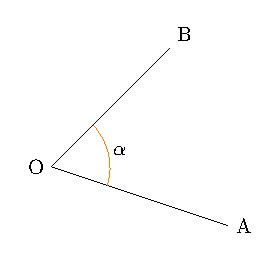
\includegraphics[scale=0.8]{Fig.ArbitraryAngle.pdf}
\end{figure}\par
{\bf 角的符号表示}:上图所示的角可记为“角AOB”、“$\angle{AOB}$”或“$\angle O$”、“角$\alpha$”或“$\angle\alpha$”
“$\alpha$”.\\
三个特殊角:{\bf\kaishu 零角,平角,直角}\par
\begin{exercise}{习题}
\item
下列说法正确的是\xz
\xx{终边相同的角一定相等}
{钝角一定是第二象限角}
{第一象限角一定不是负角}
{小于90\textdegree 的角都是锐角}
\begin{answer}B\end{answer}
\end{exercise}

\section{任意角的三角函数}
\subsection{预备知识}
1. 锐角三角函数;函数定义域
2. 勾股定理;开方;代数式化简,完全平方公式;一元二次方程求解
\subsection{问题导学}
{\heiti 【思考1】}:锐角三角函数的定义是?为什么要定义三角函数呢?三角函数有哪些应用?\par
\vspace{12em}
{\heiti 【思考2】}:锐角三角函数之间有什么关系呢?\par
\vspace{12em}

% \section{课后作业}


\stoptexercise

  % % sty文件使用 \RequirePackage{latexexercise0}
% 主文件使用 \documentclass[a3paper,twocolumn,2twoside,landscape,12pt,UTF8]{ctexart}
\hspace{3cm}\\
\vspace{0.5cm}
\centering{\heiti \xiaoer 福州八中2018-2019学年第一学期期中考试}\\
\vspace{0.5cm}
\centering{\heiti \erhao 高一数学\quad 必修一}\\
\vspace{0.4cm}
\centering{\wuhao 考试时间:120分钟\hspace{5em}试卷满分:150分}\\
\vspace{-1.6em}
\part{第I卷}
\vspace{-3em}
\startexercise
\begin{exercise}
\section{选择题(本大题共10小题,每小题5分,共50分.每题有且只有一个选项是正确的,请把答案填在答卷相应位置上)}
\item
设集合$A=\{x\in\mathbb{Q}|x>1\}$,则\xz
  \xx{$\varnothing\in A$}
  {$\sqrt2\notin A$}
  {$\sqrt2\in A$}
  {$\{\sqrt2\}\subseteq A$}
\begin{answer}
  B
\end{answer}
\item
下列函数中与函数$y=x(x\geq 0)$有相同图像的一个是\xz
  \xx{$\displaystyle y=\frac{x^2}x $}
  {$y=\sqrt{x^2}$}
  {$y=\sqrt[3]{x^3}$}
  {$y=(\displaystyle \sqrt x)^2 $}
\begin{answer}
  D
\end{answer}
\item
下列函数在区间$(0,+\infty) $上是增函数的是\xz
  \xx{$y=\ln(x+1)$}
  {$y=(x-1)^2$}
  {$y=x^{-2}$}
  {$y=3^{-x}$}
\begin{answer}
  A
\end{answer}
\item
设$f(x)=\begin{cases}
  x-2,x\geq10\\f[f(x+6)],x<10
\end{cases}$,则$f(9)$的值为\xz
  \xx{10}{11}{12}{13}
\begin{answer}
  B
\end{answer}
\item
若函数$f(x)=x^3+x^2-2x-2$的一个正数零点附近的函数用二分法计算,其参考数据如下:\\
\begin{center}
  \begin{tabular}{|c|c|c|}
    \hline
    $f(1)=-2$&$f(1.5)=0.625$&$f(1.25)=-0.984$\\
    \hline
    $f(1.375)=-0.260$&$f(1.4375)=0.162$&$f(1.40625)=-0.054$\\
    \hline
  \end{tabular}\\
\end{center}
那么方程$x^3+x^2-2x-2=0$的一个近似根(精确度$0.1$)是\xz
  \xx{1.2}
  {1.3}
  {1.4}
  {1.5}
\begin{answer}
  C
\end{answer}
\item
已知函数$f(x)$的值域为$[-2,3]$,则函数$f(x-2)$的值域为\xz
  \xx{$[-4,1]$}
  {$[0,5]$}
  {{$[-4,1]\cup[0,5]$}}
  {$[-2,3]$}
\begin{answer}
  A
\end{answer}
\item
三个数$0.8^9,9^{0.8},\log_{0.8}9$的大小关系为\xz
  \xx{$\log_{0.8}9<0.8^9<9^{0.8}$}
  {$0.8^9<9^{0.8}<\log_{0.8}9$}
  {$\log_{0.8}9<9^{0.8}<0.8^9$}
  {$0.8^9<\log_{0.8}9<9^{0.8}$}
\begin{answer}
  A
\end{answer}
\item
函数$f(x)=1+\log_2x$与$g(x)=2^{-(x-1)}$在同一直角坐标系下的图像大致是\xz
\begin{tikzpicture}
  \coordinate[label=below left:$O$] (O) at(0,0);
  \draw[->,>=latex](-0.8,0)--(3.6,0)node[below](x){$x$};
  \draw[->,>=latex](0,-1.5)--(0,3.2)node[left](y){$y$};
  \draw[domain=0.4:3]plot(\x,{log2(\x)});
  \draw[domain=-0.5:3]plot(\x,{pow(2,1-\x)});
  \draw[dashed](1,0.1)--(1,0)node[below](x1){$ 1 $};
  \draw[dashed](2,0.1)--(2,0)node[below](x2){$ 2 $};
  \draw[dashed](0.1,1)--(0,1)node[left](y1){$ 1 $};
  \draw[dashed](0.1,2)--(0,2)node[left](y2){$ 2 $};
  \coordinate[label=$\mathrm{A}$](a) at(1.5,-2);
  \begin{scope}[xshift=4.7 cm]
    \coordinate[label=below left:$O$] (O) at(0,0);
    \draw[->,>=latex](-0.8,0)--(3.6,0)node[below](x){$x$};
    \draw[->,>=latex](0,-1.5)--(0,3.2)node[left](y){$y$};
    \draw[domain=0.4:3]plot(\x,{0.1+log2(\x)});
    \draw[domain=-0.7:3]plot(\x,{pow(2,-\x)});
    \draw[dashed](1,0.1)--(1,0)node[below](x1){$ 1 $};
    \draw[dashed](2,0.1)--(2,0)node[below](x2){$ 2 $};
    \draw[dashed](0.1,1)--(0,1)node[left](y1){$ 1 $};
    \draw[dashed](0.1,2)--(0,2)node[left](y2){$ 2 $};
    \coordinate[label=$\mathrm{B}$](a) at(1.5,-1.8);
  \end{scope}
  \begin{scope}[xshift=9.4 cm]
    \coordinate[label=below left:$O$] (O) at(0,0);
    \draw[->,>=latex](-0.8,0)--(3.6,0)node[below](x){$x$};
    \draw[->,>=latex](0,-1.5)--(0,3.2)node[left](y){$y$};
    \draw[domain=0.2:3]plot(\x,{1+log2(\x)});
    \draw[domain=-0.5:3]plot(\x,{pow(2,1-\x)});
    \draw[dashed](1,0.1)--(1,0)node[below](x1){$ 1 $};
    \draw[dashed](2,0.1)--(2,0)node[below](x2){$ 2 $};
    \draw[dashed](0.1,1)--(0,1)node[left](y1){$ 1 $};
    \draw[dashed](0.1,2)--(0,2)node[left](y2){$ 2 $};
    \coordinate[label=$\mathrm{C}$](a) at(1.5,-1.8);
  \end{scope}
  \begin{scope}[xshift=14.1 cm]
    \coordinate[label=below left:$O$] (O) at(0,0);
    \draw[->,>=latex](-0.8,0)--(3.6,0)node[below](x){$x$};
    \draw[->,>=latex](0,-1.5)--(0,3.2)node[left](y){$y$};
    \draw[domain=0.3:3]plot(\x,{0.98+log2(\x)});
    \draw[domain=-0.7:2]plot(\x,{pow(3,\x-1)});
    \draw[dashed](1,0.1)--(1,0)node[below](x1){$ 1 $};
    \draw[dashed](2,0.1)--(2,0)node[below](x2){$ 2 $};
    \draw[dashed](0.1,1)--(0,1)node[left](y1){$ 1 $};
    \draw[dashed](0.1,2)--(0,2)node[left](y2){$ 2 $};
    \coordinate[label=$\mathrm{D}$](a) at(1.5,-1.8);
  \end{scope}
\end{tikzpicture}
\\
\begin{answer}
  C
\end{answer}
\item
已知函数$f(x)=x^2-2x+3$在区间$[0,t]$上的最大值为3,最小值为2,则实数$t$的取值范围是\xz
  \xx{$[1,2]$}
  {$(0,1]$}
  {$[1,+\infty)$}
  {$(0,2]$}
\begin{answer}
  A
\end{answer}
\item
某公司为激励创新,计划逐年加大研发资金投入.若该公司2015年全年投入研发资金130万元,在此基础上,每年投入的研发资金比上一年增长$12\%$.则该公司全年投入的研发资金开始超过200万元的年份是
(参考数据:$\lg1.12\approx0.05,\lg1.3\approx0.11,\lg2\approx0.30$)\xz
  \xx{2018年}
  {2019年}
  {2020年}
  {2021年}
\begin{answer}
  B
\end{answer}
\par
\section{填空题(本大题共3小题,每小题5分,共15分)}
\item
 函数$y=\sqrt{3x-1}+\lg(1-x)$的定义域是\tk
\begin{answer}
  $[\frac13 +\infty)$
\end{answer}
\item
 若函数$f(x)=(m-1)x^m$是幂函数,则函数$g(x)=\log_a(x-m)+m$(其中$a>0,a\neq 1$)的图像恒过定点$A$的坐标为\tk
 \begin{answer}
   $(3,2)$
 \end{answer}
\item
 定义在$\mathbb{R}$的偶函数$f(x)$满足:对任意的$x_1,x_2\in(\infty,0]$($x_1\neq x_2$),有
$(x_2-x_1)[f(x_2)-f(x_1)]<0$,且$f(2)=0$,则不等式$\frac{3f(x)+f(-x)}{5x}<0$的解集是\tk
\begin{answer}
  $(-\infty,-2)\cup (0,2)$
\end{answer}
\section{解答题(本大题共有3个小题,共35分. 解答应写出文字说明、演算步骤或证明过程)}
\item
(本小题满分10分)计算:\\
(I)若$x\log_52=1$求$2^x+2^{-x}$的值;\\
(II)求值$0.125^{\frac{1}3}-(-\frac78)^0+[(-2)^3]^{-\frac43}+\frac{3}4\lg 25+\lg(2\sqrt2)$.\\
\begin{answer}
  解:(I) 由$x\log_5 2=1$,$x=\frac{1}{\log_5 2}=\log_2 5$.故\\
  $2^x+2^{-x}=5+\frac15=\frac{26}5$\\
  (II)
  \begin{equation*}
    \begin{align}
      \text{原式}
      &=(\frac18)^{\frac13}-1+2^4+\frac32\lg{5}+\frac32\lg2\\
      &=\frac12+15+\frac32(\lg5+\lg2)\\
      &=17
    \end{align}
  \end{equation*}
\end{answer}
\vspace{3cm}
\item
(本小题满分10分)\\
设集合$A=\{x|2\leq x\leq4\}$,$B=\{x|0<\ln x<1\}$,$C=\{x|t+1<x<2t,t\in\mathbb{R}\}$.\\
(I)求$A\cap B$\\
(II)求$A\cap C=C$,求$t$的取值范围.\\
\begin{answer}
解:(I)$\because$ $B=\{x|1<x<\mathrm{e}\}$,$\therefore$$A\cup B=\{x|2\leq x<\mathrm{e}\}$\\
(II)$\because$ $A\cup C=C$,$\therefore$ $C\subseteq A$\\
$C=\varnothing$时,$t+1\geq 2t$,$t\leq 1$\\
$C\neq\varnothing$时,
$\begin{cases}
  t+1<2t\\
  t+1\geq 2\\
  2t\leq 4
\end{cases}
$
$\therefore$ $1<t\leq 2$\\
综上,$t\in (-\infty,2]$
\end{answer}
\vspace{4cm}
\item
(本小题满分15分)\\
已知函数$f(x)=\frac{ax+b}{x^2+1}$($a,b$是常数)是定义在$(-1,1)$上的奇函数,且$f(\frac{1}2)=\frac{2}5$.\\
(I)确定$f(x)$的解析式;\\
(II)当$x\in(-1,1)$时,判断函数$f(x)$的单调性,并用定义法证明;\\
(III)解关于$x$的不等式$f(2x-1)+f(x)<0$.\\
\begin{answer}
  解:(I)$\because$$f(x)$是奇函数,$\therefore$ $b=0$;$\because$ $f(\frac12)=\frac25$,$\therefore$ $a=1$\\
  $\therefore$ $f(x)=\frac{x}{x^2+1}$\\
  (II)$x\in(-1,1)$时,$f(x)$单调递增.证明如下:\\
  $\forall x_1,x_2\in(-1,1),x_1<x_2$,\\
  \begin{equation*}
    \begin{align*}
      f(x_2)-f(x_1)
      &=\frac{x_2}{x_2^2+1}-\frac{x_1}{x_1^2+1}\\
      &=\frac{(x_2-x_1)(1-x_1x_2)}{(x_1^2+1)(x_2^2+1)}
    \end{align*}
  \end{equation*}
   $\because x_1,x_2\in(-1,1)$,$\therefore x_1x_2<1$,即$1-x_1x_2>0$,又$x_2-x_1>0$,$x_1^2+1>0,x_2^2+1>0$\\
  $\therefore f(x_2)-f(x_1)<0$,故$f(x)$在$(-1,1)$上单调递增.\\
  (III)$\because f(x)$是奇函数,$\therefore f(2x-1)<-f(x)=f(-x)$,又$f(x)$在$(-1,1)$单调递减,故\\
  $2x-1<-x$,即$x<\frac13$;\\
  综上,$x\in (0,\frac13)$
\end{answer}
\vspace{-2em}
\part{第II卷}
\vspace{-1.5em}
\section{选择题(本大题共4小题,每小题4分,共16分.每题有且只有一个选项是正确的,请把答案填在答卷相应位置上)}
\item
函数$y=f(x)$是函数$y=a^x(a>0,a\neq1)$的反函数,且$f(2)=1$,则$f(8)=$\xz
  \xx{3}{$\frac13$}{-3}{$-\frac13$}
\begin{answer}
  A
\end{answer}
\item
若$f(x)=-x^2+2ax$与$g(x)=\frac{a}{x+1}$在区间$[1,2]$上都是减函数,则$a$的取值范围是\xz
  \xx{$(-1,0)\cup (0,1)$}
  {$(-1,0)\cup (0,1]$}
  {$(0,1)$}
  {$(0,1]$}
\begin{answer}
  D
\end{answer}
\item
对于集合$M,N$,定义$M-N=\{x|x\in M,\text{且}x\notin N$,$M\oplus N=(M-N)\cup(N-M)$,设$A=\{x|x\geq-\frac{9}4\}$,$B=\{x|x<0\}$,则$A\oplus B=$\xz
  \xx{$(-\frac{9}4,0]$}
  {$[-\frac{9}4,0)$}
  {$(-\infty,-\frac{9}4)\cup[0,+\infty)$}
  {$(-\infty,-\frac{9}4]\cup(0,+\infty)$}
\begin{answer}
  C
\end{answer}
\item
用$\max\{a,b,c\}$表示$a,b,c$三个数中的最大值,设$f(X)=\max\{2^x,x+2,10-x\},(x\leq 0)$,则$f(x)$取得最小值时$x$所在的区间为\xz
  \xx{$(1,2)$}
  {$(2,3)$}
  {$(3,4)$}
  {$(4,5)$}
\begin{answer}
  B
\end{answer}
\section{填空题(本大题共2小题,每小题4分,共8分)}
\item
已知$f(x)$是定义在$\mathbb{R}$的奇函数,当$x>0$时,$f(x)=x^2-4x$,则不等式$f(x)>x$的解集用区间表示为\tk
\begin{answer}
  $(-5,0)\cup(5,+\infty)$
\end{answer}
\item
已知函数$f(x)=\begin{cases}
  a^x,x\geq 2,\\(3-a)x+2,x<2
\end{cases}$
为$\mathbb{R}$上的增函数,则实数$a$取值的范围是\tk
\begin{answer}
  $[0,2]$
\end{answer}
\section{解答题(本大题共有2个小题,共26分. 解答应写出文字说明、演算步骤或证明过程)}
\item
(本小题满分12分)\\
设二次函数$f(x)=ax^2+bx+c$的图像过点$(0,1)$和$(1,4)$,且对于任意的实数$x$,不等式$f(x)\geq 4x$恒成立.\\
(I)求函数$f(x)$的表达式;\\
(II)设$g(x)=kx+1$,若$F(x)=\log_{\frac{1}2}[g(x)-f(x)]$在区间$[2,3]$上是增函数,求实数$k$的取值范围.\\
\begin{answer}
  解:(I)$\because f(x)$过点$(0,1)$,$\therefore c=1$;又$\because f(x)$过点$(1,4)$,$\therefore a+b=3,\therefore b=3-a$,$\therefore f(x)=ax^2+(3-a)x+1$;又$f(x)\geq 4x$恒成立,即\\
  $ax^2+(3-a)x+1\geq 4x\Leftrightarrow ax^2-(a+1)x+1\geq 0$恒成立,$\therefore a>0,\Delta=(a+1)^2-4a=(a-1)^2\leq 0$,$\because (a-1)^2\geq 0$,$\therefore (a-1)^2=0,\therefore a=1$.\\
  $\therefore f(x)=x^2+2x+1$;\\
  (II) 令$h(x)=g(x)-f(x)=(kx+1)-(x^2+2x+1)=-x^2-(2-k)x$,\\
  则依题意可知$h(x)$在区间$[2,3]$上是减函数,又函数$h(x)$开口向下,对称轴$x=\frac{k-2}2$,
  $\therefore
  \begin{cases}
    \frac{k-2}2\leq 2\\
    h(3)>0
  \end{cases}$,\\
  $\therefore 5<k\leq 6$\\
\end{answer}
\vspace{7cm}
\item
(本小题满分14分)\\
已知函数$y=x+\frac{a}x$有如下性质:如 果常数$a>0$,那么该函数在$(0,\sqrt a]$上是减函数,在$[\sqrt a,+\infty)$上是增函数.\\
(I)若函数$y=x+\frac{2^b}x\;(x>0)$的值域为$[6,+\infty)$,求实数$b$的值;\\
(II)已知函数$f(x)=\frac{4x^2-12x-3}{2x+1},x\in[0,1]$,求函数$f(x)$的单调区间和值域;\\
(III)对于(II)中的函数$f(x)$和函数$g(x)=-x-2c$,若对任意$x_1\in[0,1]$,总存在$x_2\in[0,1]$,使得$g(x_2)=f(x_1)$成立,求实数$c$的值.\\
\begin{answer}
  解:(I)依题意,当$x=\sqrt{2^b}$时,函数$y=x+\frac{2^b}x$取最小值$2\sqrt{2^b}=6$,$\therefore b=\log_2 9$\\
  (II) $\because f(x)=\frac{4x^2-12x-3}{2x+1}=2x+1+\frac{4}{2x+1}-8,x\in [0,1]$, \\
  $\therefore 2x+1\in[1,3]$,且$2x+1\in(0,2]\cap [1,3]=[1,2]$时$f(x)$是减函数,$2x+1\in[2,+\infty)\cap [1,3]=[2,3]$时$f(x)$是增函数;\\
  $\therefore$$f(x)$的单调增区间为$[\frac12,1]$,单调减区间为$[0,\frac12]$,
  最小值为$2\sqrt4-8=-4$,又$f(0)=-3,f(1)=-\frac{11}3$
  $\therefore f(x)$值域为$[-4,-3]$\\
  (III) $g(x)$在$[0,1]$上单调递减,$\therefore g(x)$值域为$[-1-2c,-2c]$;\\
  依题意可得$[-4,-3]\subseteq[-1-2c,-2c]$,
  $\therefore$
  $\begin{cases}
    -4\geq -1-2c\\
    -3\leq -2c
  \end{cases}$\\
  $\therefore c=\frac32$
\end{answer}
\end{exercise}
\stopexercise
\hspace{2em}
\newpage
\part{参考答案}
\printanswer

  % % sty文件使用 \RequirePackage{latexexercise0}
% 主文件使用 \documentclass[a3paper,twocolumn,2twoside,landscape,12pt,UTF8]{ctexart}
\hspace{3cm}\\
\vspace{0.5cm}
\centering{\heiti \xiaoer 福州八中2018-2019学年第一学期末考试}\\
\vspace{0.5cm}
\centering{\heiti \erhao 高一数学\quad 必修4}\\
\vspace{0.4cm}
\centering{\wuhao 考试时间:120分钟\hspace{5em}试卷满分:150分}\\
\vspace{0.4cm}
\centering{\wuhao 命题:王芳玲\hspace{5em}审核:唐巧珍\hspace{5em}校对:陈楚\hspace{5em}2019.1.24}\\
\vspace{-1.6em}
\part{第I卷(100分)}
\vspace{-3em}
\startexercise
\begin{exercise}
\section{选择题(本大题共8小题,每小题5分,共40分.每题有且只有一个选项是正确的,请把答案填在答卷相应位置上)}
  \item
    下列说法\CJKunderdot{错误}的是\xz
      \xx{向量$\vv{AB}$与$\vv{BA}$的长度相等}
       {零向量没有方向}
       {向量不能比较大小,向量的模可以比较大小}
       {两个相等的向量若起点相同,则终点必相同}
    \begin{answer}
      B
    \end{answer}
  \item
    若角$\alpha$为第二象限角,则化简$\dfrac{|\sin\alpha|}{\sin\alpha}-\dfrac{\cos\alpha}{|\cos\alpha|}$为\xz
      \xx{$2$}{$0$}{$1$}{$-2$}
    \begin{answer}
      A
    \end{answer}
  \item
    若一扇形的弧长为2,面积为1,则该扇形的圆心角的弧度数是\xz
      \xx{4}{3}{2}{1}
    \begin{answer}
      C
    \end{answer}
  \item
    将函数$f(x)=\sin\Bp{2x+\dfrac{\piup}6}$的图像向左平移$\dfrac{\piup}6$个单位,则所得的图像对应的函数是\xz
      \xx{$y=\sin{2x}$}
       {$y=\cos{2x}$}
       {$y=\sin\Bp{2x+\dfrac{\piup}3}$}
       {$y=\cos\Bp{2x+\dfrac{2\piup}3}$}
    \begin{answer}
      B
    \end{answer}
  \item
    在边长为2的正三角形$ABC$中,$\vv{AB}\cdot\vv{BC}$为\xz
      \xx{$2\sqrt3$}
        {$-2\sqrt3$}
        {$2$}
        {$-2$}
    \begin{answer}
      D
    \end{answer}
  \item
    已知$\cos(\alpha+\beta)=-\dfrac35$,$\sin(\alpha-\beta)=\dfrac35$,且$\alpha+\beta\in\Bp{\dfrac{\piup}2,\piup}$,$\alpha-\beta\in\Bp{\dfrac{\piup}2,\piup}$,则$\cos{2\beta}$的值为\xz
      \xx{$-1$}
       {$1$}
       {$\dfrac{24}{25}$}
       {$-\dfrac{24}{25}$}
    \begin{answer}
      C
    \end{answer}
  \\\begin{minipage}[htbp!]{0.7\linewidth}\item
    如图,正方形ABCD中,点E,F分别是DC,BC的中点,那么$\vv{EF}=$\xz
    \xx{$\dfrac12\vv{AB}-\dfrac12\vv{AD}$}
     {$-\dfrac12\vv{AB}+\dfrac12\vv{AD}$}
     {$-\dfrac12\vv{AB}-\dfrac12\vv{AD}$}
     {$\dfrac12\vv{AB}+\dfrac12\vv{AD}$}
    \end{minipage}
    \begin{minipage}[htbp!]{0.25\linewidth}
      \begin{flushright}
        \vspace{-1.5em}
        \begin{tikzpicture}
          \coordinate[label=left:$A$](A)at(0,0);
          \coordinate[label=right:$B$](B)at(2,0);
          \coordinate[label=left:$D$](D)at(0,2);
          \coordinate[label=right:$C$](C)at(2,2);
          \coordinate[label=right:$F$](F)at($(C)!0.5!(B)$);
          \coordinate[label=above:$E$](E)at($(C)!0.5!(D)$);
          \draw (A)--(B)--(C)--(D)--cycle;
          \draw[->,>=latex] (A)--(B);
          \draw[->,>=latex] (A)--(D);
          \draw[->,>=latex] (E)--(F);
        \end{tikzpicture}
      \end{center}
    \end{minipage}
    \begin{answer}
      A
    \end{answer}
  \item
    已知$a=\dfrac{\sqrt2}2(\sin{18\degree}+\cos{18\degree})$,$b=2\cos^2{16\degree}-1$,$c=\dfrac{\sqrt3}2$,则\xz
    \xx{$c<a<b$}{$b<c<a$}{$a<b<c$}{$b<a<c$}
    \\
    \begin{answer}
      B
    \end{answer}
\par
\section{填空题(本大题共4小题,每小题5分,共20分)}
  \item
     在平行四边形$ABCD$中,若$\vv{AB}=(2,4)$,$\vv{AD}=(-1,-1)$,则$\vv{BD}=$\tk
    \begin{answer}
      $(-3,-5)$
    \end{answer}
  \item
     若角$\alpha$的终边过点$P\bigl(2\cos{120\degree},\sqrt2\sin(-45\degree)\bigr)$,则$\sin\alpha=$\tk
     \begin{answer}
       $-\dfrac{\sqrt2}2$
     \end{answer}
  \item
     已知函数$y=A\sin(\omega x+\varphi)$($A>0$,$\omega>0$)的振幅是$3$,频率是$\dfrac5{2\piup}$,初相是$\dfrac{\piup}6$,则这个函数是$y=$\tk
    \begin{answer}
      $3\sin\Bp{5x+\dfrac{\piup}6}$
    \end{answer}
  \item
    设$\bm a$,$\bm b$,$\bm c$为任意非零向量,且相互不共线,则下列命题中是真命题的序号为\tk\\
    (1)$|\bm a|-|\bm b|<|\bm a-\bm b|$\hspace{4em}
    (2)$(\bm a\cdot\bm b)\cdot\bm c-(\bm c\cdot\bm a)\cdot\bm b=0$\\
    (3)$(\bm b\cdot\bm c)\cdot\bm a-(\bm c\cdot\bm a)\cdot\bm b$与$\bm c$垂直\hspace{2em}
    (4)$(3\bm a+\bm b)\cdot(3\bm a-\bm b)=9|\bm a|^2-|\bm b|^2$
    \begin{answer}
      (1)(3)(4)
    \end{answer}
\section{解答题(本大题共有4个小题,共40分. 解答应写出文字说明、演算步骤或证明过程)}
  \item
    (本小题满分8分)\\
    已知$\bm a=(1,2)$,$\bm b=(x,1)$,分别求实数$x$的值使得:\\
    \circled{1} $(2\bm a+\bm b)\varparallel(\bm a-2\bm b)$;
    \circled{2} $\bm a$与$\bm b$的夹角是60\degree.
    \begin{answer}
      \circled{1} $2\bm a+\bm b=(2+x,5)$,$\bm a-2\bm b=(1-2x,0)$;
        $\because (2\bm a+\bm b)\varparallel(\bm a-2\bm b)$,
        $\therefore 0+5(1-2x)=0$,$\therefore x=\dfrac12$;\par
      \circled{2} $\bm a\cdot\bm b
        =\abs{\bm a}\abs{\bm b}\cos{60\degree}
        =\sqrt5\cdot\sqrt{x^2+1}\cdot\dfrac12=x+2$,即
        $5(x^2+1)=4(x+2)^2$,
        解得$x=8\pm 5\sqrt3$
    \end{answer}
  \vspace{4em}
  \item
    (本小题满分10分)\\
    已知$\cos\alpha-\sin\alpha=\dfrac{3\sqrt2}5$,且$\piup<\alpha<\dfrac{3\piup}2$,化简$\dfrac{\sin{2\alpha}+2\sin^2\alpha}{1-\tan\alpha}$并求其值.
    \begin{answer}
      由$\cos\alpha-\sin\alpha=\dfrac{3\sqrt2}5$,
      $\cos^2\alpha+\sin^2\alpha-2\sin\alpha\cos\alpha=\dfrac{3\sqrt2}{5}$,\\
      $\therefore 2\sin\alpha\cos\alpha=1-\dfrac{18}{25}=\dfrac7{25}$;\\
      $\therefore (\sin\alpha+\cos\alpha)^2=\sin^2\alpha+\cos^2\alpha+2\sin\alpha\cos\alpha
      =1+\dfrac7{25}=\dfrac{32}{25}$;
      又$\because \piup<\alpha<\dfrac{3\piup}2$,
      $\therefore \sin\alpha<0$,$\cos\alpha<0$,\\
      $\therefore \sin\alpha+\cos\alpha=\dfrac{4\sqrt2}5$,\\
      $\therefore \dfrac{\sin{2\alpha}+2\sin^2\alpha}{1-\tan\alpha}
      =\dfrac{2\sin\alpha\cos\alpha+2\sin^2\alpha}{1-\dfrac{\sin\alpha}{\cos\alpha}}
      =\dfrac{2\sin\alpha\cos\alpha(\sin\alpha+\cos\alpha)}{\sin\alpha+\cos\alpha}
      =\dfrac{\dfrac7{25}\cdot(-\dfrac{4\sqrt2}{5})}{\dfrac{3\sqrt2}{5}}
      =-\dfrac{28}{75}$
    \end{answer}
  \vspace{4em}
  \item
    (本小题满分10分)\\
    已知向量$\bm m=(1,1)$,向量$\bm n$与$\bm m$的夹角为$\dfrac{3\piup}4$,且$\bm m\cdot\bm n=-1$.\\
    (1)求向量$\bm n$;\\
    (2)设向量$\bm a=(1,0)$,$\bm b=(\cos x,\sin x)$,其中$x\inR$,若$\bm n\cdot\bm a=0$,试求$|\bm n+\bm b|$的取值范围.
    \begin{answer}
      (1)由$\bm m=(1,1)$,$\bm m$与x轴正半轴夹角为45\degree,
        又$\bm n$与$\bm m$的夹角为$\dfrac{3\piup}4$,故$\bm n$在$x$轴或$y$轴负半轴上,\\
        设$\bm n=(n_1,0)$或$\bm n=(0,n_2)$,又$\bm m\cdot\bm n=-1$,
        $\therefore \bm n=(-1,0)$或$(0,-1)$.\par
      (2)由$\bm n\cdot\bm a=0$,$\bm n=(0,-1)$;
        $\therefore \abs{\bm n+\bm b}=\sqrt{\cos^2x+(\sin{x}-1)^2}
        =\sqrt{\cos^2x+\sin^2x-2\sin x+1}=\sqrt{2-2\sin x} \in[0,2]$;
    \end{answer}
  \vspace{5em}
  \item
    (本小题满分12分)\\
    已知函数$f(x)=\sqrt3\cos{\omega x}$,$g(x)=\sin\Bp{\omega x-\dfrac{\piup}3}$($\omega>0$),且$g(x)$的最小正周期为$\piup$.\\
    (1)若$f(\alpha)=\dfrac{\sqrt6}2$,$\alpha\in[0,\piup]$,求$\alpha$的值;\\
    (2)求函数$y=f(x)+g(x)$的单调递增区间.
    \begin{answer}
      (1)$g(x)$的最小正周期为$\piup$,$\therefore \dfrac{2\piup}{\omega}=\piup$,
        $\there \omega=2$\\
        $\therefore f(\alpha)=\sqrt3\cos{2\alpha}=\dfrac{\sqrt6}2$,
        $\therefore 2\alpha=\pm\dfrac{\piup}4+2k\pipu$,
        $\therefore \alpha=\pm\dfrac{\piup}8+k\pipu$,$k\inZ$;\\
        又$\alpha\in[0,\piup]$,
        $\therefore$ $\alpha=\dfrac{\piup}8$或$\dfrac{7\piup}8$\par
      (2)$y=f(x)+g(x)=\sqrt3\cos{2x}+\sin\Bp{2x-\dfrac{\piup}3}
          =\dfrac12\sin{2x}+\dfrac{\sqrt3}2\cos{2x}=\sin\Bp{2x+\dfrac{\piup}3}$,\\
          由$-\dfrac12\piup+2k\piup \leqslant 2x+\dfrac{\piup}3 \leqslant \dfrac12\piup+2k\piup$,得:
          $-\dfrac{5\piup}{12}+k\piup \leqslant x \leqslant \dfrac{\piup}{12}+k\piup$,$k\inZ$;\\
          故函数$y=f(x)+g(x)$的单调递增区间为
          $\Bigl[-\dfrac{5\piup}{12}+k\piup,\dfrac{\piup}{12}+k\piup\Bigr]$,$k\inZ$
    \end{answer}
  \vspace{4em}
\newpage
\vspace{-3em}
\part{第II卷(50分)}
\vspace{-1.5em}
\section{选择题(本大题共4小题,每小题4分,共16分.每题有且只有一个选项是正确的,请把答案填在答卷相应位置上)}
  \item
    若$\cos{165\degree}=a$,则$\tan{195\degree}=$\xz
      \xx
       {$\sqrt{1-a^2}$}
       {$\dfrac{\sqrt{1+a^2}}a$}
       {$\dfrac{\sqrt{1-a^2}}a$}
       {$-\dfrac{\sqrt{1-a^2}}a$}
    \begin{answer}
      D
    \end{answer}
  \item
    已知函数$f(x)=2\sin\Bp{\omega x+\dfrac{\piup}3}$图像的一个对称中心为$\Bp{\dfrac{\piup}3,0}$,其中$\omega$为常数,且$\omega\in(1,3)$,若对任意的实数$x$,恒有$f(x_1)\leq f(x)\leq f(x_2)$,则$|x_1-x_2|$的最小值是\xz
      \xx{$1$}{$\dfrac{\piup}2$}{$2$}{$\piup$}
    \begin{answer}
      B
    \end{answer}
  \item
    已知$O$是$\triangle{ABC}$所在平面上一点,满足$|\vv{OA}|^2+|\vv{BC}|^2=|\vv{OB}|^2+|\vv{CA}|^2$,则点$O$\xz
      \xx{在过点$C$与$AB$垂直的直线上}
       {在$\angle{A}$的平分线所在直线上}
       {在过点$C$边$AB$的中线所在直线上}
       {以上都不对}
    \begin{answer}
      A
    \end{answer}
  \item
    目前听说中国最高的摩天轮是“南昌之星”,它的最高点离地面160米,直径为156米,并以每30分钟一周的速度匀速旋转,若从最低点开始计时,则摩天轮运行5分钟后离地面的高度为\xz
      \xx{31米}{43米}{58米}{63米}
    \begin{answer}
      B
    \end{answer}
\section{填空题(本大题共2小题,每小题4分,共8分)}
  \item
    若函数$f(x)=\tan{\omega x}$($\omega>0$)的图像相邻的两支截直线$y=\dfrac{\piup}4$所得线段的长为$\dfrac{\piup}4$,则$f(\dfrac{\piup}4)$的值是\tk
    \begin{answer}
      $0$
    \end{answer}
  \item
    在矩形$ABCD$中,边$AB$、$AD$的长分别为2、1,若$M$、$N$分别是边$BC$、$CD$上的点,且满足$\dfrac{|\vv{BM}|}{|\vv{BC}|}=\dfrac{|\vv{CN}|}{|\vv{CD}|}$,则$\vv{AM}\cdot\vv{AN}$的取值范围是\tk
    \begin{answer}
      $[1,4]$
    \end{answer}
\newpage
\section{解答题(本大题共有2个小题,共26分. 解答应写出文字说明、演算步骤或证明过程)}
  \item
    (本小题满分12分)\\
    已知$O$为$\triangle{ABC}$的外心,以线段$OA$、$OB$为邻边作平行四边形,第四个顶点为$D$,再以$OC$、$OD$为邻边作平行四边形,它的第四个顶点为$H$.\\
    (1) 若$\vv{OA}=\bm a$,$\vv{OB}=\bm b$,$\vv{OC}=\bm c$,$\vv{OH}=\bm h$,试用$\bm a$,$\bm b$,$\bm c$表示$\bm h$;\\
    (2)证明:$\vv{AM}\perp\vv{BC}$;\\
    (3)若$\triangle{ABC}$的$\angle{A}=60\degree$,$\angle{B}=45\degree$,外接圆的半径为$R$,用$R$表示$|\bm h|$.
    \begin{answer}
      (1)$\bm h=\bm a+\bm b+\bm c$\par
      (2)\because $\vv{AH}=\vv{OH}-\vv{OA}=\bm b+\bm c$,$\vv{BC}=\bm c-\bm b$.\\
         \therefore $\vv{AH}\cdot\vv{BC}=|\bm c|^2-|\bm b|^2=0$,\\
         \therefore $\vv{AH}\perp\vv{BC}$.\par
      (3)\because$|\bm h|^2=(\bm a+\bm b+\bm c)^2=3R^2+2R^2(\cos120\degree+\cos90\degree+\cos150\degree)=(2-\sqrt3)R^2$,\\
         \therefore $|\bm h|=\dfrac{\sqrt6-\sqrt2}2 R$
    \end{answer}
  \vspace{12em}
  \item
    (本小题满分14分)\\
    已知函数$f(x)=2\cos x\sin\Bp{x+\dfrac{\piup}3}-\sqrt3\sin^2x+\sin x\cos x$\\
    (1) 当$x\in\Bigl[0,\dfrac{\piup}2\Bigr]$时,求$f(x)$的值域;\\
    (2) 解不等式:$f(x)+1\geq 0$;\\
    (3) 若$x\in\Bigl[0,\dfrac{\piup}3\Bigr]$时,方程$f\Bp{\dfrac32x-\dfrac{\piup}3}=m$恰有两个不同的解,求实数$m$的取值范围
    \begin{answer}
      (1) $f(x)=2\cos x\sin\Bp{x+\dfrac{\piup}3}-\sqrt3\sin^2x+\sin x\cos x
               =2\cos x(\dfrac12\sin x+\dfrac{\sqrt3}2\cos x)-\sqrt3\sin^2x+\sin x\cos x
               =\sin{2x}+\sqrt3\cos{2x}
               =2\sin\Bp{2x+\dfrac{\piup}3}$,\\
          故$x\in\Bigl[0,\dfrac{\piup}2\Bigr]$时,$2x+\dfrac{\piup}3 \in\Bigl[\dfrac{\piup}3,\dfrac{4\piup}4\Bigr]$,\\
          $f(x)$值域为$[-\sqrt3,2]$;\par
      (2) 由$f(x)+1\geq 0$,得$\sin\Bp{2x+\dfrac{\piup}3}\geq -\dfrac12$\\
          $\therefore -\dfrac{\piup}6+2k\piup \leqslant 2x+\dfrac{\piup}3 \leqslant \dfrac{7\piup}{6}+2k\piup$,$k\inZ$;\\
          $\therefore \Bigl[-\dfrac{\piup}4+k\piup,\dfrac{5\piup}{12}+k\piup \Bigr]$,$k\inZ$;\par
      (3) $x\in\Bigl[0,\dfrac{\piup}3\Bigr]$时,$f\Bp{\dfrac32x-\dfrac{\piup}3}=2\sin\Bp{3x-\dfrac{\piup}3}$,
          \begin{center}
            \begin{tikzpicture}[>=latex,,scale=1,declare function={f(\k)=2*sin(deg(3*\k-pi/3));}]
              \tikzmath{
                \xmin = 0;    \xmax = pi/3;
                \ymin = -2;   \ymax = 2;
                \xstep= pi/6; \ystep=1;
                \xl=\xmin-0.5*\xstep; \xr=\xmax+0.5*\xstep;
                \yl=\ymin-0.5*\ystep; \yr=\ymax+0.5*\ystep;
              }
              % \tikzset{elegant/.style={smooth,thick,samples=50,magenta}}
              \begin{axis}[axis x line=middle,
                     axis y line=middle,
                     xmin=\xl,xmax=\xr,
                     ymin=\yl,ymax=\yr,
                     % xstep=\xstep,ystep=\ystep,
                     xtick={0,1,2},
                     ytick distance=\ystep,
                     ylabel=$y$,
                     xlabel=$x$]
                    \addplot[elegant,orange,domain=0:1]{f(x)};
                    \addplot[elegant,dashed,domain=0:\xstep]{2};
                    \addplot[elegant,dashed,domain=\xl:\xr]{1.732};
                    % \draw[dashed] (0,2)node[left](a){$2$}-|(\a,0)node[below](a1){$\dfrac{5\pi}{12}$};
              \end{axis}
              % \draw[->](\xl,0)--(\xr,0) node[below](x){$x$};
              % \draw[->](0,\yl)--(0,\yr) node[left](y){$y$};
              % \node[below left](O) at(0,0){$\small O$};
              % \draw[domain=\xmin:\xmax,samples=300] plot (\x,{f(\x)});
              % \draw[dashed] (0,2)node[left](a){$2$}-|(\a,0)node[below](a1){$\dfrac{5\pi}{12}$} ;;
              % \draw[dashed](0,-2)node[left](b){$-2$}-|(\b,0)node[above](b1){$\dfrac{11\pi}{12}$} ;
            \end{tikzpicture}
          \end{center}
          $\therefore 3x-\dfrac{\piup}3\in\Bigl[-\dfrac{\piup}3,\dfrac{2\piup}3\Bigr]$,\\
          故方程$f\Bp{\dfrac32x-\dfrac{\piup}3}=m$恰有两个不同的解时,$m\in\Bigl[2\sin\dfrac{2\piup}3,2\Bigr]$,即\\
          $m\in[\sqrt3,2)$;
    \end{answer}
  \vspace{8em}
\end{exercise}
\stopexercise
\hspace{2em}
\clearpage
\hspace{3cm}\\
\vspace{-2.5em}
\part{\heiti \xiaoer 参考答案}
\begin{multicols}{2}
  \printanswer
\end{multicols}

  % % sty文件使用 \RequirePackage{latexexercise0}
% 主文件使用 \documentclass[a3paper,twocolumn,2twoside,landscape,12pt,UTF8]{ctexart}
% \hspace{3cm}\\
% \vspace{0.5cm}
% \part{\centering{\heiti \xiaoer 福州清大教育2018-2019学年高一数学期末考模拟卷}}\\
\twocolumn
\part{\mbox{\heiti \xiaoer 福州清大教育2018-2019学年高一数学期末考模拟卷}}
  % \vspace{-1.5cm}
  \centering{\heiti \erhao 高一数学\quad 必修四}\\
  \centering{\wuhao (考试时间:120分钟,满分:150分,另附加分30分)}\\
  \vspace{-1.6em}
  \startexercise
  \begin{exercise}
  \section{选择题(本大题共12小题,每小题5分,共60分.每题有且只有一个选项是正确的,请把答案填在答卷相应位置上)}
    \item%福州三中2016-2017学年第二学期高一数学期末考试-1【弧度制与角度制】
      关于角度制与弧度制的等式,正确的是\xz
      \xx{$\piup=1\rm{rad}$}
        {$\piup=180$}
        {$1^{\degree}=\dfrac{180}{\piup}\rm{rad}$}
        {$1\rm{rad}=\Bigl(\dfrac{180}{\piup}\Bigr)^\degree$}
      \begin{answer}
        D
      \end{answer}
    \item%格致中学2015-2016学年第四学段高一期末考试-3【任意角三角函数】
      已知$\tan\alpha=-\sqrt3,0<\alpha<\piup$,那么$\cos\alpha-\sin\alpha$的值是\xz
      \xx{$-\dfrac{1+\sqrt3}2$}
        {$\dfrac{-1+\sqrt3}2$}
        {$\dfrac{1-\sqrt3}2$}
        {$\dfrac{1+\sqrt3}2$}
      \begin{answer}
        A
      \end{answer}
    \item%LaTeX-master/xiangliang/xiangliangsorting.tex 练习P7-10【向量共线、线性运算】
      设$ D $为$\triangle ABC$所在平面内一点,$ \vv{BC}=3\vv{CD} $,则\xz
      \xx{$ \vv{AD}=-\dfrac{1}{3}\vv{AB}+\dfrac{4}{3}\vv{AC}$}
        {$ \vv{AD}=\dfrac{1}{3}\vv{AB}-\dfrac{4}{3}\vv{AC}$}
        {$ \vv{AD}=\dfrac{4}{3}\vv{AB}+\dfrac{1}{3}\vv{AC}$}
        {$ \vv{AD}=\dfrac{4}{3}\vv{AB}-\dfrac{1}{3}\vv{AC}$}
      \begin{answer}
        A
      \end{answer}
    \item%LaTeX-master/2018/qimo.tex-7【Asin(\omega x+\varphi)】
      函数$f(x)=2\sin\left(\omega x+\varphi\right)\left(\omega>0,\abs{\varphi}<\dfrac{\pi}{2}\right)$的部分图象如图所示,则$ \omega,\varphi $的值分别是\xz
      \begin{minipage}[b]{0.7\linewidth}
        \vspace{1.5cm}
        \xx{$ 2,-\dfrac{\pi}{3}$}{$2,-\dfrac{\pi}{6} $}{$4,-\dfrac{\pi}{6} $}{$ 4,\dfrac{\pi}{3}$}
      \end{minipage}\hfill
      \begin{minipage}[h]{0.3\linewidth}
        \vspace{-1cm}
        \begin{tikzpicture}[>=latex,scale=1]
          \tikzmath{
            \a = 5*pi/12;
            \b=11*pi/12;
          }
          \draw[->](-1,0)--(4,0) node[below](x){$x$};
          \draw[->](0,-2.3)--(0,2.3) node[left](y){$y$};
          \node[below left](O) at(0,0){$\small O$};
          \draw[domain=0:pi,samples=1000] plot (\x,{2*sin((2*(\x)-pi/3) r)});
          \draw[dashed] (0,2)node[left](a){$2$}-|(\a,0)node[below](a1){$\dfrac{5\pi}{12}$} ;;
          \draw[dashed](0,-2)node[left](b){$-2$}-|(\b,0)node[above](b1){$\dfrac{11\pi}{12}$} ;
          %\draw[dashed] (0,2)-|($(5*pi/12,0)$);
        \end{tikzpicture}
      \end{minipage}
      \begin{answer}
        A
      \end{answer}
    \item%《习题化知识清单》P85方法3-4.1【向量夹角垂直】
      向量$\bm a=(1,-2),\bm b=(2,1)$,则\xz
      \xx{$\bm a\varparallel \bm b$}
        {$\bm a\perp \bm b$}
        {$\bm a$与$\bm b$的夹角为$60\degree$}
        {$\bm a$与$\bm b$的夹角为$30\degree$}
      \begin{answer}
        B
      \end{answer}
    \item%《习题化知识清单》P84知识5-23【数量积应用,三角形五心】
      点$O$是$\triangle{ABC}$所在平面上的一点,且满足$\vv{OA}\cdot\vv{OB}=\vv{OB}\cdot\vv{OC}=\vv{OA}\cdot\vv{OC}$,则点$O$是$\triangle{ABC}$的\xz
        \xx{重心}
          {垂心}
          {内心}
          {外心}
      \begin{answer}
        B
      \end{answer}
    \item%《习题化知识清单》P71知识-4【诱导公式】
      已知$\sin{\Bigl(\dfrac{\piup}3+\alpha\Bigr)}=-\dfrac{5}{13}$,则$\cos{\Bigl(\dfrac{\piup}6-\alpha \Bigr)}=$\xz
      \xx{$-\dfrac{5}{12}$}
        {$\dfrac{5}{13}$}
        {$-\dfrac{5}{13}$}
        {$\dfrac{1}{5}$}
      \begin{answer}
        C
      \end{answer}
    \item%《习题化知识清单》P89知识3-3【三角恒等变换,综合】
      若$\alpha\in(0,\piup)$,且$\cos\alpha+\sin\alpha=-\dfrac{1}{3}$,则$\cos{2\alpha}$等于\xz
        \xx{$\dfrac{17}9$}
          {$\pm\dfrac{17}9$}
          {$-\dfrac{17}9$}
          {$\dfrac{17}3$}
      \begin{answer}
        A
      \end{answer}
    \item%《习题化知识清单》P90单元检测10【数量积;三角恒等变换,综合】
      已知向量$\bm a=\Bigl(\cos\dfrac{3x}2,\sin\dfrac{3x}2\Bigr)$,$\bm b=\Bigl(\cos\dfrac{x}2,-\sin\dfrac{x}2\Bigr)$,且$x\in\Bigl[0,\dfrac{\piup}2\Bigr]$,
      若$\abs{\bm a+\bm b}=2\bm a\cdot\bm b$,则$\sin{2x}+\tan{x}=$\xz
      \xx{$-1$}{$0$}{$2$}{$-2$}
      \begin{answer}
        B
      \end{answer}
    \item%《习题化知识清单》P75方法2.3【三角函数图像】
      设函数$f(x)=\sin{\Bigl(2x+\dfrac{\piup}3\Bigr)}$,则下列结论正确的是\xz
      \xx{$f(x)$的图像关于直线$x=\dfrac{\piup}3$对称}
        {$f(x)$的图像关于点$\Bigl(-\dfrac{\piup}4,0\Bigr)$对称}
        {把$f(x)$的图像向左平移$\dfrac{\piup}{12}$个单位长度,得到一个偶函数的图像}
        {$f(x)$的最小正周期为$\piup$,且在$\Bigl[0,\dfrac{\piup}6 \Bigr]
        $上为增函数}
      \begin{answer}
        C
      \end{answer}
    \item%《习题化知识清单》P90单元检测8【向量投影】
      在平面直角坐标系中,$AB=CD$,$A(0,3)$,$B(-4,0)$,$C(a,-1)(a>0)$,则向量$\vv{BC}$在$\vv{AB}$上的投影为\xz
        \xx{$-5$}
          {$-3$}
          {$3$}
          {$5$}
      \begin{answer}
        A
      \end{answer}
    \item%《习题化知识清单》P90单元检测9【三角恒等变换,二次方程】
      已知$\tan\alpha$,$\tan\beta$是方程$x^2-3x-5=0$的两根,则$\tan{2(\alpha+\beta)}$的值为\xz
        \xx{$-\dfrac{24}{25}$}
          {$\dfrac{24}7$}
          {$-\dfrac{4}{5}$}
          {$-\dfrac{4}{3}$}
      \begin{answer}
        D
      \end{answer}
    \item%《高中数学竞赛培优教程+一试(李名德 主编)》.pdf P122-5.2-3
      (附加题,5分)
      已知正方形$PQRS$对角线交点为$M$,坐标原点$O$不在正方形内部,$\vv{OP}=(0,3)$,$\vv{OS}=(4,0)$,则向量$\vv{RM}$为\xz
      \xx{$\Bigl(-\dfrac{7}{2},-\dfrac{1}{2}\Bigr)$}
        {$\Bigl(\dfrac{7}{2},\dfrac{1}{2}\Bigr)$}
        {$(7,4)$}
        {$\Bigl(\dfrac{7}{2},\dfrac{7}{2}\Bigr)$}
      \begin{answer}
        A
      \end{answer}
    \item%《高中数学竞赛培优教程+一试(李名德 主编)》.pdf P92-4.1-4
      (附加题,5分)
      已知$\theta\in[0,\piup]$,$f(x)=\sin{(\cos\theta)}$的最大值为$a$,最小值为$b$,$g(\theta)=\cos{(\sin\theta)}$的最大值为$c$,最小值为$d$,则$a,b,c,d$从小到大的顺序是\xz
      \xx{$b<d<a<c$}
        {$d<b<c<a$}
        {$b<d<c<a$}
        {$d<b<a<c$}
      \begin{answer}
        A
      \end{answer}
  \section{填空题(本大题共4小题,每小题5分,共20分)}
    \item%《习题化知识清单》P84方法1-1【向量夹角,参数】
       已知$\abs{\bm a}=1,\abs{\bm b}=2$,$\bm a$与$\bm b$的夹角为$120\degree$,则使$\bm a+k\bm b$与$k\bm a+\bm b$的夹角为锐角的实数$k$的取值范围是\tk[5].
      \begin{answer}
        $\Bigl(\dfrac{5-\sqrt{21}}2,1\Bigr)\bigcup\Bigl(1,\dfrac{5+\sqrt{21}}2\Bigr)$
      \end{answer}
    \item%《习题化知识清单》P70方法3.2【同角三角函数关系化简】
      已知$\sin\alpha\cos\alpha=-\dfrac{12}{25}$,$\alpha\in\Bigl(-\dfrac{\piup}4,0\Bigr)$,则$\sin\alpha+\cos\alpha=$\tk.
      \begin{answer}
        $\dfrac{1}{5}$
      \end{answer}
    \item%《习题化知识清单》P85方法4-5.2【数量积,数形结合】
       已知正方形$ABCD$的边长为1,点$E$是$AB$边上的动点,则$\vv{DE}\cdot\vv{DC}$的最大值为\tk.
       \begin{answer}
         1
       \end{answer}
    \item%《习题化知识清单》P89方法1-1【三角恒等变换,函数性质】
       已知函数$f(x)=\dfrac{(\sin x-\cos x)\sin {2x}}{\sin x}$,则$f(x)$的单调递减区间为\tk[6].
      \begin{answer}
        $\Bigl[k\piup+\dfrac{3\piup}8,k\piup+\dfrac{7\piup}8\Bigr](k\in\mathbb{Z})$
      \end{answer}
    \item%《高中数学奥林匹克竞赛解题方法大全(周沛耕 主编)》.pdf P93例3
      (附加题,5分)
      $\sqrt3\tan{18\degree}+\tan{18\degree}\tan{12\degree}+\sqrt3\tan{12\degree}=$\tk.
      \begin{answer}
        1
      \end{answer}
  % \clearpage
  \section{解答题(本大题共有6个小题,共70分. 解答应写出文字说明、演算步骤或证明过程)}
    \item
      (本小题满分10分)求值:\\
      已知$\abs{\vv a}=\sqrt2,\abs{\vv{\mathstrut b}}=1$
      (1)若$\vv a,\vv b$的夹角$\theta$为$45\degree$,求$\abs{\vv{\mathstrut a}-\vv{\mathstrut b}}$;\\
      (2)若$(\vv{\mathstrut a}-\vv{\mathstrut b})\perp \vv{\mathstrut b}$,求$\vv{\mathstrut a}$与$\vv{\mathstrut b}$的夹角$\theta$.
      \begin{answer}
        解:(1) $\abs{\vv a-\vv b}=\sqrt{\vv a^2-2\vv a\!\cdot\!\vv b+\vv b^2}=\sqrt{2-2\times\sqrt2\times1\times\dfrac{\sqrt2}2+1}=1$\fz[5]
        (2)$\because(\vv a-\vv b)\perp\vv b$,\\
        $\therefore(\vv a-\vv b)\cdot\vv b=\vv a\cdot\vv b-\vv b^2=\sqrt2\times1\times\cos\theta-1=0$,\\
        $\therefore\cos\theta=\dfrac{\sqrt2}2(0\le\theta\le\piup)$,$\therefore\theta=\dfrac{\piup}4.$\fz[10]
      \end{answer}
    \vspace{3cm}
    \clearpage
    \item
      (本小题满分12分)\par
      (1)化简:$\dfrac{\cos{\Bigl(\alpha-\dfrac{\piup}2\Bigr)}}{\sin{\Bigl(\dfrac{5\piup}2+\alpha\Bigr)}}\cdot\sin{(\alpha-2\piup)}\cdot\cos{(\piup-\alpha)}$;\\
      (2)已知$\tan{a}=-2$,求$\dfrac{\sin{2a}-\cos^2{a}}{2+\cos{2a}}$的值.
      \begin{answer}
      解:(1)$\text{原式}=\dfrac{\sin\alpha}{\cos\alpha}\cdot\sin\alpha\cdot(-\cos\alpha)=-\sin^2\alpha$;\\
      (2)$\because\tan\alpha=-2$,
      $\therefore\text{原式}=\dfrac{2\sin\alpha\cdot\cos\alpha-\cos^2\alpha}{2\cos^2\alpha+1}
      =\dfrac{2\sin\alpha\cdot\cos\alpha-\cos^2\alpha}{3\cos^2\alpha+\sin^2\alpha}
      =\dfrac{\dfrac{2\sin\alpha\cdot\cos\alpha-\cos^2\alpha}{\cos^2\alpha}}{\dfrac{3\cos^2\alpha+\sin^2\alpha}{\cos^2\alpha}}
      =\dfrac{2\tan\alpha-1}{3+\tan^2\alpha}=\dfrac{2\times(-2)-1}{3+(-2)^2}
      =-\dfrac{5}{7}.$
      \end{answer}
    \vspace{3cm}
    \item
      (本小题满分12分)\\
      设函数$f(x)=\bm a\cdot\bm b$,其中向量$\bm a=(\cos x,1)$,$\bm b=\bigl(\cos x,\sqrt3\sin x\cos x\bigr)$,$x\in\mathbb{R}$.\\
      (1)求函数$f(x)$的解析式;\\
      (2)求满足$f(x)\leqslant0$的$x$的集合;\\
      (3)函数$y=\sin x$的图像可由函数$y=f(x)$的图像经过怎样的变换得到?\\
      \begin{answer}
        解:(1)$f(x)=\bm a\cdot\bm b
        =\cos^2x+\sqrt3\sin x\cos x
        =\dfrac{\cos{2x}+1}2+\dfrac{\sqrt3}{2}\sin{2x}
        =\sin{\Bigl(2x+\dfrac{\piup}6\Bigr)}+\dfrac12.$\\
        (2)$\because f(x)\leqslant0$,
        $\therefore \sin{\Bigl(2x+\dfrac{\piup}6\Bigr)}\leqslant-\dfrac12.$\\
        又$\because$不等式$\sin x\leqslant-\dfrac12$的解集为$\Bigl[2k\piup-\dfrac{5\piup}6,2k\piup-\dfrac{\piup}6\Bigr],k\in\mathbb{Z}.$\\
        $\therefore 2k\piup-\dfrac{5\piup}6 \leqslant 2x+\dfrac{\piup}6 \leqslant 2k\piup-\dfrac{\piup}6$.\\
        解得:$k\piup-\dfrac{\piup}2 \leqslant x \leqslant k\piup-\dfrac{\piup}6$
        即:函数$f(x)\leqslant0$的$x$的解集为$\Bigl\{x\Bigm| k\piup-\dfrac{\piup}2 \leqslant x \leqslant k\piup-\dfrac{\piup}6,k\in\mathbb{Z}\Bigr\}$.\\
        (3)函数$y=\sin x$的图像可由函数$y=f(x)$的图像经过以下步骤变换得到:\\
        $\circled{1}$向下平移$\dfrac12$个单位,得到函数$y=\sin{\Bigl(2x+\dfrac{\piup}6\Bigr)}$的图像;\\
        $\circled{2}$向右平移$\dfrac{\piup}{12}$个单位,得到函数$y=\sin {2x}$的图像;\\
        $\circled{3}$横坐标伸长2倍,得到函数$y=\sin x$的图像.
      \end{answer}
    \vspace{3.6cm}
    \item
      (本小题满分12分)\\
      已知函数$f(x)=2\sin^2{\Bigl(\dfrac{\piup}4+x\Bigr)}+\sqrt3\cos{2x}$.\\
      (1)求函数$f(x)$的最小正周期和对称轴方程;\\
      (2)若关于$x$的方程$f(x)-m=2$在$x\in\Bigl[0,\dfrac{\piup}2\Bigr]$上有两个不同的解,求实数$m$的取值范围.\\
      \begin{answer}
        【分析】(1)利用三角函数的倍角公式以及辅助角公式将函数进行化简即可求最小正周期和对称轴方程;\\
        (2)求出函数$f(x)$在$x\in\Bigl[0,\dfrac{\piup}2\Bigr]$的取值情况,利用数形结合即可得到结论.\\
        【解答】解:(1)由$f(x)=2\sin^2{\Bigl(\dfrac{\piup}4+x\Bigr)}+\sqrt3\cos{2x}
        =1-\cos{\Bigl(\dfrac{\piup}2+2x\Bigr)}+\sqrt3\cos{2x}
        =1+\sin{2x}+\sqrt3\cos{2x}=1+2\sin{\Bigl(\dfrac{\piup}3+2x\Bigr)}$,\\
        $\because \omega=2$,$\therefore$函数$f(x)$的最小正周期为$\piup$.\\
        由$2x+\dfrac{\piup}3=\dfrac{\piup}2+k\piup,k\in\mathbb{Z}$得:$x=\dfrac{\piup}{12}+\dfrac12k\piup,{k\in\mathbb{Z}}$,\\
        故函数$f(x)$的对称轴方程为:$x=\dfrac{\piup}{12}+\dfrac12k\piup,{k\in\mathbb{Z}}$.\\
        (2)由$f(x)-m=2$得$f(x)=m+2$,\\
        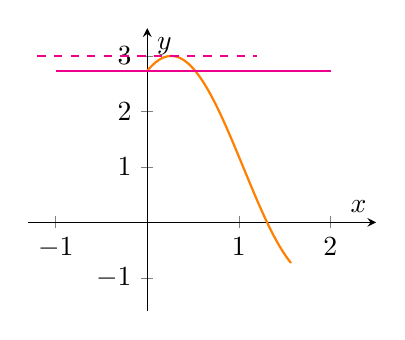
\begin{tikzpicture}[declare function={f(\k)=1+2*sin(deg(2*\k+pi/3));}]
          \tikzset{elegant/.style={smooth,thick,samples=50,magenta}}
          \begin{axis}[axis x line=middle,
                 axis y line=middle,
                 xmin=-1.3,xmax=2.5,
                 ymin=-1.6,ymax=3.5,
                 xstep=1,ystep=1,
                 ytick distance=1,
                 ylabel=$y$,
                 xlabel=$x$]
                \addplot[elegant,orange,domain=0:pi/2]{f(x)};
                \addplot[elegant,dashed,domain=-1.2:1.2]{3};
                \addplot[elegant,domain=-1:2]{2.732};
          \end{axis}
        \end{tikzpicture}
        当${x\in\Bigl[0,\dfrac{\piup}2\Bigr]}$时,$2x+\dfrac{\piup}3\in\Bigl[\dfrac{\piup}3,\dfrac{4\piup}3\Bigr]$,\\
        由图象得$f(0)=1+2\sin{\dfrac{\piup}3}=1+\sqrt3$,\\
        函数$f(x)$的最大值为$1+2=3$,\\
        $\therefore$要使方程$f(x)-m=2$在$x\in\Bigl[0,\dfrac{\piup}2\Bigr]$上有两个不同的解,
        则$f(x)=m+2$在$x\in\Bigl[0,\dfrac{\piup}2\Bigr]$上有两个不同的解,\\
        即函数$f(x)$和$y=m+2$在$x\in\Bigl[0,\dfrac{\piup}2\Bigr]$上有两个不同的交点,\\
        即$1+\sqrt3\leqslant m+2<3$,\\
        即 $\sqrt3-1\leqslant m<1$.
      \end{answer}
    \vspace{3.6cm}
    \item
      (本小题满分12分)\\
      已知向量$\bm a=\Bigl(\dfrac{1}2,\sin x\Bigr)$,$\bm b=\biggl(-1,\cos{\Bigl(x-\dfrac{\piup}6\Bigr)}\biggr)$,$f(x)=\bm a\cdot\bm b+\dfrac{1}4$,$(x\in\mathbb{R})$.\\
      (1)求函数$f(x)$的单调递减区间;\\
      (2)若函数$g(x)=f(x)-m,\Bigl(\dfrac{\piup}3\leqslant x\leqslant\dfrac{13\piup}{12}\Bigr)$有两个不同的零点$x_1,x_2$,求实数$m$的取值范围及$x_1,x_2$的和.\\
      \begin{answer}
        解:(1)$f(x)=\bm a\cdot\bm b+\dfrac{1}4
        =-\dfrac12+\sin{x}\cdot\cos{\Bigl(x-\dfrac{\piup}6\Bigr)}+\dfrac14
        =\sin{x}\cdot \Bigl(\cos x\cos{\dfrac{\piup}6}+\sin x\sin{\dfrac{\piup}6}\Bigr)-\dfrac14
        =\dfrac{\sqrt3}2\sin x\cos x+\dfrac12\sin^2x-\dfrac14
        =\dfrac{\sqrt3}4\sin{2x}-\dfrac14\cos{2x}
        =\dfrac12\sin{\Bigl(2x-\dfrac{\piup}6\Bigr)}$.\\
        由$2x-\dfrac{\piup}6\in\Bigl[\dfrac{\piup}2+2k\piup,\dfrac{3\piup}2+2k\piup\Bigr]$,${k\in\mathbb{Z}}$,解得$x\in\Bigl[\dfrac{\piup}3+k\piup,\dfrac{5\piup}6+k\piup\Bigr]$,${k\in\mathbb{Z}}$.\\
        $\therefore$函数$f(x)$的单调递减区间为$\Bigl[\dfrac{\piup}3+k\piup,\dfrac{5\piup}6+k\piup\Bigr]$,${k\in\mathbb{Z}}$.\\
        (2) $\because$函数$g(x)=f(x)-m,\Bigl(\dfrac{\piup}3\leqslant x\leqslant\dfrac{13\piup}{12}\Bigr)$有两个不同的零点$x_1,x_2$,
        $\therefore$函数$y=f(x)$的图像与函数$y=m$的图像在$\Bigl[\dfrac{\piup}3,\dfrac{13\piup}{12}\Bigr]$上有两个交点.\\
        又$\because \dfrac{\piup}3\leqslant x\leqslant\dfrac{13\piup}{12}$,
        $\therefore 2x-\dfrac{\piup}6\in\Bigl[\dfrac{\piup}2,2\piup\Bigr]$.
      \end{answer}
    \vspace{4cm}
    \item
      (本小题满分12分)\\
      如图,某污水处理厂要在一个矩形污水处理池($ABCD$)的池底水平铺设污水净化管道($Rt\triangle{FHE}$,$H$是直角顶点)米处理污水,管道越长,污水净化效果越好。设计要求管道的接口$H$是$AB$的中点,$E$、$F$分别落在线段$BC$、$AD$上.已知$AB=20$米,$AD=10\sqrt3$米,记$\angle{BHE}=\theta$.\\
      (1)试将污水净化管道的长度$l$表示为$\theta$的函数,并写出定义域;\\
      (2)若$\sin\theta+\cos\theta=\sqrt2$,求此时管道的长度$l$;\\
      (3)当$\theta$取何值时,污水净化效果好?并求出此时管道的长度.\\
      \begin{flushleft}
        \begin{tikzpicture}
          \coordinate[label=left:$A$](A)at(0,0);
          \coordinate[label=right:$B$](B)at(4,0);
          \coordinate[label=left:$D$](D)at(0,3.5);
          \coordinate[label=right:$C$](C)at(4,3.5);
          \draw[dashed] (A)rectangle(C);
          \coordinate[label=below:$H$](H)at(2,0);
          \coordinate[label=right:$E$](E)at(4,3);
          \path[name path=AD] (A)--(D);
          % \coordinate (P)at($(H)!2!90:(E)$);
          \path[name path=PH] ($(H)!1!90:(E)$)--(H);
          \path[name intersections={of=AD and PH}];
          \coordinate[label=left:$F$] (F)  at (intersection-1);
          % \draw[red] ($(H)!6pt!(E)$)--($(H)!6pt!(E)!6pt!90:(E)$)--($(H)!6pt!(F)$);
          \draw \rAm{E}{H}{F};
          % \draw [--] ($(H)+(0.5,0)$) arc (0:30:1cm);
          % \node at ($(H)+(0.8,0.3)$) {$\theta$};
          % \pic["\alpha",draw=red,angle radius=0.5cm] {angle=A--B--C};
          \path (B)--(H)--(E) pic [draw,"$\theta$",angle eccentricity=1.5] {angle=B--H--E};
          \draw (H)--(E)--(F)--cycle;
        \end{tikzpicture}
      \end{flushleft}
      \begin{answer}
        解:
      \end{answer}
    \vspace{1.5cm}
    \item%福州格致中学2015-2016学年高一数学第二学期期末检测.docx-22
      (附加题:本小题满分15分)\\
      (福州格致中学2015-2016学年高一数学第二学期期末检测22)已知函数$f(x)=A\sin(\omega x+\varphi)+B (A>0,\omega>0)$的一系列对应值如下表:
      \begin{center}
        \renewcommand{\arraystretch}{1.4}
        \begin{tabular}{|*{8}{c|}}
          \hline
            $x$
            &$\dfrac{\piup}6$
            &$-\dfrac{\piup}3$
            &$-\dfrac{5\piup}6$
            &$-\dfrac{4\piup}3$
            &$-\dfrac{11\piup}6$
            &$-\dfrac{7\piup}3$
            &$-\dfrac{17\piup}6$\\
          \hline
            $y$
            &$-1$
            &$1$
            &$3$
            &$1$
            &$-1$
            &$1$
            &$3$\\
          \hline
        \end{tabular}\\
      \end{center}
      (1)根据表格提供的数据求函数$f(x)$的一个解析式;\\
      (2)根据(1)的结果:\\
      \;(i)当$x\in\Bigl[0,\dfrac{\piup}3\Bigr]$时,方程$f(3x)=m$恰有两个不同的解,求实数$m$的取值范围;\\
      \;(ii)若是$\alpha,\beta$是锐角三角形的两个内角,试比较$f(\sin \alpha)$与$f(\cos \beta)$的大小.
      \begin{answer}
        (1)$f(x)=2\sin\Bigl(x-\dfrac{\piup}3\Bigr)+1$;(2)(i)$[\sqrt{3}+1,3)$;(ii)易得$f(x)$在$[-\dfrac{\piup}6,\dfrac{5\piup}6]$上单调递增,故$f(x)$在$[0,1]$上单调递增;又$0<\dfrac{\piup}2-\beta<\alpha<\dfrac{\piup}2$,从而$\sin\alpha>\sin(\dfrac{\piup}2-\beta)=\cos\beta$,于是$f(\sin \alpha)>f(\cos \beta)$
      \end{answer}
    \vspace{4cm}
  \end{exercise}
  \stopexercise
\newpage
\centering{\heiti \xiaoer 福州清大教育2018-2019学年高一数学期末考模拟卷}\\
\part{\mbox{\heiti \xiaoer 参考答案}}
  \begin{multicols}{2}
    \printanswer
  \end{multicols}

  % % sty文件使用 \RequirePackage{latexexercise0}
% 主文件使用 \documentclass[a3paper,twocolumn,2twoside,landscape,12pt,UTF8]{ctexart}
\hspace{3cm}\\
\vspace{0.5cm}
\centering{\heiti \xiaoer 福州三中2018-2019学年第二学期半期考}\\
% \vspace{0.5cm}
\centering{\heiti \xiaoer 高一\quad 数学试卷}\\
\vspace{0.4cm}
\rightline{\wuhao 命题人:高一数学集备组\hspace{3em}}\\
\rightline{\wuhao 审卷人:黄炳锋\hspace{7em}}\\
\begin{flushleft}
  \wuhao 注意事项:\\
  1. 答卷前,考生务必将自己的姓名、准考证号填写在试卷和答题卡上。\\
  2. 回答选择题时,用铅笔把答题卡上对应题目的答案标号涂黑,如需改动,用橡皮檫干净后,再选涂其他答案标号。回答非选择题时,将答案写在答题卡上,写在本试卷上无效。
\end{flushleft}
\vspace{-1.6em}
\part{第I卷}
\vspace{-3em}
\startexercise
\begin{exercise}
\section{选择题(本大题共12小题,每小题5分,共60分.在每小题给出的四个选项中,只有一个选项是符合题目要求的.}
  \item%福州三中2018-2019学年高一数学期中考试卷.pdf p1
    % \source{2019}{福州三中 1}
    若$a,b,c\inR$,且$a>b$,则下列不等式一定成立的是\xz
      \xx{$a+c\geqslant b-c$}
       {$(a-b)c^2\geqslant0$}
       {$\mfrac{c^2}{a-b}>0$}
       {$ac>bc$}
    \begin{answer}
      B
    \end{answer}
  \item%福州三中2018-2019学年高一数学期中考试卷.pdf p2
    % \source{2019}{福州三中 2}
    在正方体$ABCD-A_1B_1C_1D_1$中,异面直线$AD_1$与$BD$所成角的大小为\xz
    \xx{30\degree}{45\degree}{60\degree}{90\degree}
    \begin{answer}
      C
    \end{answer}
  \item%福州三中2018-2019学年高一数学期中考试卷.pdf p3
    % \source{2019}{福州三中 3}
    已知等差数列$\{a_n\}$中,$a_3=3$,$a_7=1$,则$a_{11}$等于\xz
    \xx{$-2$}{$-1$}{$1$}{$2$}
    \begin{answer}
      B
    \end{answer}
  \item%福州三中2018-2019学年高一数学期中考试卷.pdf p4
    % \source{2019}{福州三中 4}
    设$M=2a(a-2)$,$N=(a+1)(a-3)$,则有\xz
    \xx{$M>N$}{$M=N$}{$M<N$}{$M$与$N$大小不定}
    \begin{answer}
      A
    \end{answer}
  \item%福州三中2018-2019学年高一数学期中考试卷.pdf p5
    % \source{2019}{福州三中 5}
    Rt$\triangle{ABC}$中,$\angle{CAB}=90\degree$,$AB=3$,$AC=4$,以$AC$所在直线为轴将$\triangle{ABC}$旋转一周,所得几何体的体积等于\xz
      \xx{$8\piup$}{$12\piup$}{$24\piup$}{$36\piup$}
    \begin{answer}
      B
    \end{answer}
  \item%福州三中2018-2019学年高一数学期中考试卷.pdf p6
    % \source{2019}{福州三中 6}
    在$\triangle{ABC}$中,角$A$,$B$,$C$的对边分别为$a$,$b$,$c$,若$A=60\degree$,$a=\sqrt3$,$b=1$,则$c$等于\xz
      \xx{$1$}{$2$}{$\sqrt3-1$}{$3$}
    \begin{answer}
      B
    \end{answer}
  \item%福州三中2018-2019学年高一数学期中考试卷.pdf p7
    % \source{2019}{福州三中 7}
    首项为$-24$的等差数列从第10项起开始为正数,则公差$d$的取值范围是\xz
      \xx{$\Bigl(\mfrac83,+\infty\Bigr)$}
       {$(-\infty,3)$}
       {$\Bigl[\mfrac83,3\Bigr)$}
       {$\Bigl(\mfrac83,3\Bigr]$}
    \begin{answer}
      D
    \end{answer}
  \item%福州三中2018-2019学年高一数学期中考试卷.pdf p8
    % \source{2019}{福州三中 8}
    在$\triangle{ABC}$中,已知$\sin^2A+\sin^2B-\sin A \sin B=\sin^2C$,且满足$ab=4$,则$\triangle{ABC}$的面积为\xz
      \xx{$1$}{$2$}{$\sqrt3$}{$2\sqrt3$}
    \begin{answer}
      C
    \end{answer}
  \item%福州三中2018-2019学年高一数学期中考试卷.pdf p9
    % \source{2019}{福州三中 9}
    由实数构成的等比数列$\{a_n\}$的前$n$项和为$S_n$,$a_1=2$,且$a_2-4$,$a_3$,$a_4$成等差数列,则$S_6$等于\xz
    \xx{62}{124}{126}{154}
    \begin{answer}
      C
    \end{answer}
  \clearpage
  \item%福州三中2018-2019学年高一数学期中考试卷.pdf p10
    % \source{2019}{福州三中 10}
    已知不等式$(x+y)\Bp{\mfrac1x+\mfrac{a}y}\geqslant9$对任意正实数$x$,$y$恒成立,则正实数$a$的最小值为\xz
    \xx{6}{5}{4}{3}
    \begin{answer}
      C
    \end{answer}
  \item%福州三中2018-2019学年高一数学期中考试卷.pdf p11
    % \source{2019}{福州三中 11}
    如图所示,位于$A$处的信息中心获悉:在其正东方向相距40 n mile 的$B$处有一艘渔船遇险,在原地等待救援,信息中心立即把消息告知在其正南偏西30\degree,相距20 n mile $C$处的乙船,乙船立即沿直线$CB$前往救援,则$\sin\angle{ACB}$等于\xz
    \begin{minipage}[t]{0.5\linewidth}\vspace{-0.5\baselineskip}
      \xx{$\mfrac{\sqrt{21}}7$\hspace{5em}}
       {$\mfrac{\sqrt{21}}{14}$\hspace{5em}}
       {$\mfrac{\sqrt5}7$\hspace{5em}}
       {$\mfrac{\sqrt5}{14}$\hspace{5em}}
    \end{minipage}
    \begin{minipage}[t]{0.5\linewidth}\vspace{-0.5\baselineskip}
      \begin{flushright}\begin{tikzpicture}[scale=0.8]
        \coordinate[label=above left:$A$] (A) at(0,0);
        \coordinate[label=right:$B$] (B) at(4,0);
        \coordinate[label=below:$C$] (C) at(-1,-1.73);
        % \draw (A)--(B)--(C)--cycle;
        \draw (A)--node[anchor=south]{40 n mile}(B);
        \draw (A)--node[anchor=east]{20 n mile}(C) (B)--(C);
        \draw [dashed] ($(A)+(0,-2)$)--++(0,2.7);
        \draw [->,>=latex] ($(B)+(0,0.3)$)--node[anchor=west]{北} ++(0,0.8);
        \end{tikzpicture}
      \end{flushright}
    \end{minipage}
    \begin{answer}
      A
    \end{answer}
  \item%福州三中2018-2019学年高一数学期中考试卷.pdf p12
    % \source{2019}{福州三中 12}
    已知四棱锥$S-ABCD$的所有顶点都在同一球面上,底面$ABCD$是矩形且和球心$O$在同一平面内,若此四棱锥的最大体积为$\mfrac{16}3$,则球$O$的表面积等于\xz
    \xx{$8\piup$}{$16\piup$}{$32\piup$}{$64\piup$}
    \begin{answer}
      B
    \end{answer}
\vskip
\part{第II卷}
\vspace{-1em}
\section{填空题:本题共4小题,每小题5分,共20分.}
  \item%福州三中2018-2019学年高一数学期中考试卷.pdf p13
    % \source{2019}{福州三中 13}
    已知数列$\{a_n\}$的前$n$项和为$S_n=n^2+3n-2$,则$a_6=$\tk.
    \begin{answer}
      14
    \end{answer}
  \item%福州三中2018-2019学年高一数学期中考试卷.pdf p1
    % \source{2019}{福州三中 14}
    已知正$\triangle{ABC}$的边长为2,则由斜二测画法画出的直观图的面积为\tk.
     \begin{answer}
       $\mfrac{\sqrt6}4$
     \end{answer}
  \item%福州三中2018-2019学年高一数学期中考试卷.pdf p15
    % \source{2019}{福州三中 15}
    若不等式$2x-x^2\geqslant a$对一切的$x\in(-1,3]$成立,则实数$a$的取值范围为\tk.
    \begin{answer}
      $(\infty,3]$
    \end{answer}
  \item%福州三中2018-2019学年高一数学期中考试卷.pdf p16
   % \source{2019}{福州三中 16}
   在$\triangle{ABC}$中,$B=60\degree$,点$M$为$BC$中点,且$AM=AC$,则$\sin\angle{BAC}=$\tk.
   \begin{answer}
     $\mfrac{\sqrt{21}}4$
   \end{answer}
\section{解答题:本题共6小题,共70分. 解答应写出文字说明、证明过程或演算步骤.}
  \item%福州三中2018-2019学年高一数学期中考试卷.pdf p17
    % \source{2019}{福州三中 17}
    (本小题满分10分)\\
    已知锐角三角形$ABC$的角$A$,$B$,$C$的对边分别为$a$,$b$,$c$,$a=2b\sin A$.\\
    (I)求角$B$的大小;\\
    (II)若$a=3\sqrt3$,$c=5$,求$b$的值.
    \begin{answer}
      【解】:
      (I)由$a=2b\sin A$,根据正弦定理得$\sin A=2\sin B\sin A$,\\
         所以$\sin B=\mfrac12$,由$\triangle{ABC}$为锐角三角形得\\
         $B=\mfrac{\piup}6$.\\
      (II)根据余弦定理,得\\
          $b^2=a^2+c^2-2ac\cos B=27+25-45=7$.\\
          $\therefore$ $b=\sqrt7$
    \end{answer}
  \clearpage
  \item%福州三中2018-2019学年高一数学期中考试卷.pdf p18
    % \source{2019}{福州三中 18}
    (本小题满分12分)\\
    已知不等式$ax^2-3x+2<0$的解集为$\{x\mid 1<x<b\}$.\\
    (I)求实数$a$,$b$的值;\\
    (II)解关于$x$的不等式$(b-a)x^2-(ac+b)x+2ac\geqslant0$($c\inR$).
    \begin{answer}
      【解】:
      (I)依题意,$1$与$b$是方程$ax^2-3x+2=0$的两个实数根.
         $\therefore$ $\left\{\begin{aligned}
             &1+b=\mfrac{a}3\\
             &1\times b=\mfrac2a
           \end{aligned}\right.$,解得$\left\{\begin{aligned}
               &a=1\\
               &b=2
             \end{aligned}\right.$\\
      (II)将$a$、$b$值代入可得不等式$x^2-(2+c)x+2c\geqslant0$.
         即$(x-2)(x-c)\geqslant0$.\\
         当$c=2$时, 原不等式解集为$\RR$:\\
         当$c>2$时, 原不等式解集为$(-\infty,2]\cup[c,+\infty)$;\\
         当$c<2$时, 原不等式解集为$(-\infty,c]\cup[2,+\infty)$.
    \end{answer}
  \vspace{5cm}
  \item%福州三中2018-2019学年高一数学期中考试卷.pdf p19
    % \source{2019}{福州三中 19}
    (本小题满分12分)\\
    如图所示,正方体$ABCD-A_1B_1C_1D_1$的棱长为2,$E$、$F$分别是$BC$、$C_1D_1$的中点.\\
    \begin{minipage}[t]{0.7\linewidth}
      \vspace{-0.5\baselineskip}
      (I)求异面直线$AC$与$A_1F$所成角的余弦值;\\
      (II)求证:$EF\varparallel\text{平面}BB_1D_1D$.
    \end{minipage}
    \begin{minipage}[t]{0.3\linewidth}
      \vspace{-0.5\baselineskip}
      \begin{flushright}\begin{tikzpicture}[scale=0.25,line width=0.5 pt]
        %\draw[help lines,very thin](0,0) grid (6,6);
        \tikzmath{
        \w=12;\d=12;\h=12;%宽度width,深度depth,高度height
        \arcwd=30;\arcwh=90;%直观图中 x y轴夹角;x、z轴夹角;
        \hh=\h*cos(\arcwh);
        \hv=\h*sin(\arcwh);
        \dh =\d/2*cos(\arcwd);
        \dv =\d/2*sin(\arcwd);
        }
        \coordinate[label=below:\footnotesize$A$] (A) at(0,0);
        \coordinate[label=below:\footnotesize$B$] (B) at(\w,0);
        \coordinate[label=below:\footnotesize$D$] (D) at($(A)+(\dh,\dv)$);
        \coordinate[label=below:\footnotesize$C$] (C) at($(B)+(\dh,\dv)$);
        \foreach \p in{C,D}
        \coordinate[label=above:\footnotesize$\p_1$] (\p_1) at($(\p)+(\hh,\hv)$);
        \foreach \p in{A,B}
        \coordinate[label=below left:\footnotesize$\p_1$] (\p_1) at($(\p)+(\hh,\hv)$);
        \draw (A)--(B)--(C) (A)--(A_1) (B)--(B_1) (C)--(C_1);
        \draw (A_1)--(B_1)--(C_1)--(D_1)--cycle;
        \draw[dashed] (A)--(D)--(C) (D_1)--(D);
        \coordinate[label=below right:\footnotesize$E$](E) at($(B)!0.5!(C)$);
        \coordinate[label=above:\footnotesize$F$](F) at($(C_1)!0.5!(D_1)$);
        \draw (A)--(C) (A_1)--(F) (B_1)--(D_1);
        \draw[dashed] (B)--(D) (E)--(F);
        % \foreach \p in{A,D}
        % \coordinate[label=left:\footnotesize$\p_1$] (\p_1) at($(\p)+(0,3)$);
        \end{tikzpicture}
      \end{flushright}
    \end{minipage}
    \begin{answer}
      【解】:
      \begin{center}\vspace{-1em}\begin{tikzpicture}[t,scale=0.16,line width=0.5 pt]
        %\draw[help lines,very thin](0,0) grid (6,6);
        \tikzmath{
        \w=12;\d=12;\h=12;%宽度width,深度depth,高度height
        \arcwd=30;\arcwh=90;%直观图中 x y轴夹角;x、z轴夹角;
        \hh=\h*cos(\arcwh);
        \hv=\h*sin(\arcwh);
        \dh =\d/2*cos(\arcwd);
        \dv =\d/2*sin(\arcwd);
        }
        \coordinate[label=below:\footnotesize$A$] (A) at(0,0);
        \coordinate[label=below:\footnotesize$B$] (B) at(\w,0);
        \coordinate[label=below:\footnotesize$D$] (D) at($(A)+(\dh,\dv)$);
        \coordinate[label=below:\footnotesize$C$] (C) at($(B)+(\dh,\dv)$);
        \foreach \p in{C,D}
        \coordinate[label=above:\footnotesize$\p_1$] (\p_1) at($(\p)+(\hh,\hv)$);
        \foreach \p in{A,B}
        \coordinate[label=below left:\footnotesize$\p_1$] (\p_1) at($(\p)+(\hh,\hv)$);
        \draw (A)--(B)--(C) (A)--(A_1) (B)--(B_1) (C)--(C_1);
        \draw (A_1)--(B_1)--(C_1)--(D_1)--cycle;
        \draw[dashed] (A)--(D)--(C) (D_1)--(D);
        \coordinate[label=below right:\footnotesize$E$](E) at($(B)!0.5!(C)$);
        \coordinate[label=above:\footnotesize$F$](F) at($(C_1)!0.5!(D_1)$);
        \draw (A)--(C) (A_1)--(F) (B_1)--(D_1);
        \draw[dashed] (B)--(D) (E)--(F);
        \coordinate[label=below:\footnotesize$O$] (O) at($(B)!0.5!(D)$);
        \draw[dashed] (A_1)--(C_1) (O)--(D_1) (O)--(E);
        % \foreach \p in{A,D}
        % \coordinate[label=left:\footnotesize$\p_1$] (\p_1) at($(\p)+(0,3)$);
        \end{tikzpicture}
      \end{center}\vspace{-1.2em}
      (1)连结$A_1C$,则$A_1C_1\varparallel AC$,异面直线$AC$与$A_1F$所成角为$\angle{FA_1C_1}$.\\
         $F$是$C_1D_1$的中点,$\therefore$ $D_1F=FC_1=\mfrac12C_1D_1=1$,\\
         在$\triangle{FA_1C_1}$中,$A_1C_1=\sqrt2C_1D_1=2\sqrt2$,$FC_1=1$,$A_1F=\sqrt{A_1D_1^2+D_1F^2}=\sqrt5$\\
         故由余弦定理得:\\
         $\cos\angle{FA_1C_1}=\mfrac{A_1F^2+A_1C_1^2-C_1F^2}{2A_1F\cdot A_1C_1}
          =\mfrac{5+8-1}{2\times\sqrt5\times2\sqrt2}=\mfrac{3\sqrt{10}}{10}$,\\
         即异面直线$AC$与$A_1F$所成角的余弦值为$\mfrac{3\sqrt{10}}{10}$;\\
      (II)记$AC\cap BD=O$,则$OE\varpareq\mfrac12CD\varpareq \mfrac12C_1D_1$,即$OE\varpareq D_1F$,\\
          $\therefore$ 四边形$D_1FEO$为平行四边形,$\therefore$ $EF\varparallel OD_1$,\\
          又$OD_1\subset \text{平面}BB_1D_1D$,$EF\nsubset \text{平面}BB_1D_1D$,\\
          $\therefore$ $EF\varparallel\text{平面}BB_1D_1D$.
    \end{answer}
  \vspace{2cm}
  \item%福州三中2018-2019学年高一数学期中考试卷.pdf p20
    % \source{2019}{福州三中 20}
    (本小题满分12分)\\
    已知等比数列$\{a_n\}$的各项均为正数,且$a_2-2a_1=3$,$9a_3^2=a_2a_6$.\\
    (I)求数列$\{a_n\}$的通项公式;\\
    (II)设$b_n=\log_3a_1+\log_3a_2+\cdots+\log_3a_n$,求数列$\Bigl\{\mfrac1{b_n}\Bigr\}$的前$n$项和.
    \begin{answer}
      【解】:
      (I)设等比数列$\{a_n\}$的公比为$q$,则由$\{a_n\}$的各项均为正数,$q>0$.\\
         故由$9a_3^2=a_2a_6=a_4^2$得$q=\mfrac{a_4}{a_3}=3$(负值舍去).\\
         $\therefore$ $a_2-2a_1=a_1q-2a_1=a_1=3$\\
         $\therefore$ $a_n=a_1q^{n-1}=3^n$\\
      (II)$b_n=\log_3a_1+\log_3a_2+\cdots+\log_3a_n=1+2+\cdots+n=\mfrac{n(n+1)}2$.\\
          $\therefore$ $\mfrac1{b_n}=\mfrac{n(n+1)}2=2\Bp{\mfrac1n-\mfrac1{n+1}}$.\\
          $\therefore$ 记数列$\Bigl\{\mfrac1{b_n}\Bigr\}$的前$n$项和为$T_n$,则\\
          $T_n=2\Bp{1-\mfrac12}+2\Bp{\mfrac12-\mfrac13}+\cdots+2\Bp{\mfrac1n-\mfrac1{n+1}}
           =2\Bp{1-\mfrac1{n+1}}=\mfrac{2n}{n+1}$,$n\inN^*$.\\
    \end{answer}
  \clearpage
  \item%福州三中2018-2019学年高一数学期中考试卷.pdf p21
    % \source{2019}{福州三中 21}
    (本小题满分12分)\\
    $\triangle{ABC}$的三个内角$A$,$B$,$C$的对边分别为$a$,$b$,$c$,满足$(2b-c)\cos A=a\cos C$.\\
    (I)求$A$的值;\\
    (II)若$a=2$,求$\triangle{ABC}$周长的最大值.
    \begin{answer}
      【解】:
      (I)由正弦定理,$(2\sin B-\sin C)\cos A=\sin A \cos C$,\\
         $\therefore$ $2\sin B\cos A=\sin A \cos C+\sin C \cos A=\sin(A+C)=\sin B$\\
        $\therefore$ $\cos A=\mfrac12$, $\therefore$ $A=\mfrac{\piup}3$\\
      (II)由余弦定理 $4=b^2+c^2-2bc\cos\mfrac{\piup}3
          =b^2+c^2-bc=(b+c)^2-3bc\geqslant \mfrac14(b+c)^2$(当且仅当$b=c$时取等号).\\
          故$b+c\leqslant4$,$\therefore$ $a+b+c\leqslant6$\\
          即$\triangle{ABC}$周长的最大值为6.
    \end{answer}
  \vspace{7cm}
  \item%福州三中2018-2019学年高一数学期中考试卷.pdf p22
    % \source{2019}{福州三中 22}
    (本小题满分12分)\\
    某工艺品生产企业,拟在2019年度进行系列促销活动.经市场调查和测算,该企业一款新产品的年销售量$x$(单位:万件)与年促销费用$t$(单位:万元)之间满足$3-x$于$t+1$成反比例.若不搞促销活动,该新产品的年销售量只有1万件.已知该企业2019年生产这款新产品的固定投资为3万元,每生产1万件这款新产品需另外投资32万元.当企业把这款新产品每件的售价定为“年平均每件生产成本的1.5倍”与“年平均每件所占促销费用的一半”之和时,则当年的产量和销量相等.(利润$=$收入$-$生产成本$-$促销费用)\\
    (I)把该企业2019年的年利润$y$(单位:万元)表示成年促销费用$t$(单位:万元)的函数;\\
    (II)当2019年的促销费用投入多少万元时,该企业的年利润最大?并求出利润的最大值.
    \begin{answer}
      【解】:
      (I)设反比例系数为$k$($k\neq0$),有$3-x=\mfrac{k}{t+1}$.\\
        $\because$ $t=0$时,$x=1$,代入上式得$k=2$,\\
        $\therefore$ $x=3-\mfrac2{t+1}$($t\geqslant0$);\\
        故年利润$y=x\cdot\Bp{\mfrac{3+32x}x\cdot1.5+\mfrac{t}{2x}}-(3+32x)-t
                 =\mfrac12\Bp{99-\mfrac{64}{t+1}-t}$($t\geqslant0$).\\
      (II)$y=\mfrac12\bigl(99-\mfrac{64}{t+1}-t\bigr)
            =\mfrac12\Bigl[100-\bigl(t+1+\mfrac{64}{t+1}\bigr)\Bigr]
            \leqslant \mfrac12\Bp{100-2\sqrt{(t+1)\cdot\mfrac{64}{t+1}}}=42$,\\
          当且仅当$t+1=\mfrac{64}{t+1}$即$t=7$时(负值舍去)取等号;\\
          所以当2019年的促销费用投入$7$万元时,该企业的年利润最大,最大利润为$43$万元.
    \end{answer}

\end{exercise}
\stopexercise
\hspace{2em}
\newpage
\part{参考答案}
\begin{multicols}{2}
  \printanswer
\end{multicols}

  % % sty文件使用 \RequirePackage{latexexercise0}
% 主文件使用 \documentclass[a3paper,twocolumn,2twoside,landscape,12pt,UTF8]{ctexart}
\hspace{3cm}\\
\vspace{0.5cm}
\centering{\heiti \xiaoer 福州格致中学2020-2021学年第一学段高一数学半期考(A)}\\
\vspace{0.5cm}
% \centering{\heiti \erhao 高一数学\quad 必修4}\\
\vspace{0.4cm}
\centering{\wuhao 命题:郑鹏宇\hspace{5em}审核:金声\hspace{5em}日期:2020年11月}\\
\vspace{0.4cm}
\centering{\wuhao 考试时间:120分钟\hspace{5em}全卷满分:150分}\\
\vspace{-1.6em}
% \part{第I卷(100分)}
% \vspace{-3em}
\startexercise
\begin{exercise}
\section{单项选择题:本题共8小题,每小题5分,共40分.在每小题给出的四个选项中,只有一项是符合题目要求的}
  \item
    已知集合$A=\{x\in\mathbb{N}\mid -1\leq x \leq 4\}$,$B\{x\mid -2\leq x \leq 3\}$,则$A\cap B=$\xz
    \xx{$[-1,3]]$}
      {$[-2,4]]$}
      {$\{0,1,2,3\}$}
      {$\{1,2,3\}$}
    \begin{answer}
      
    \end{answer}
  \item
    命题“$\forall x\geq0,x^2-1\geq-1$”的否定是\xz
      \xx{$\forall x\geq0,x^2-1<-1$}
      {$\forall x<0,x^2-1<-1$}
      {$\exists x\geq0,x^2-1<-1$}
      {$\exists x<0,x^2-1<-1$}
    \begin{answer}
      
    \end{answer}
  \item
    设函数$f(x)=\begin{cases}
      2^x+m,x\leqslant0,\\
      g(x),x>0.
    \end{cases}$是奇函数,则$f(2)=$\xz
      \xx{$\frac34$}{$-\frac34$}{$4$}{$-4$}
    \begin{answer}
      
    \end{answer}
  \item 
    “$0<a<4$”是“关于$x$的方程$ax^2+ax+1=0$无实根”的\xz
      \xx{充分不必要条件}
       {必要不充分条件}
       {充要条件}
       {既不充分也不必要条件}
    \begin{answer}
      
    \end{answer}
  \item
    已知$x=2^{0.6}$,$y=\log_{1.2}2.4$,$y=\log_{1.2}3.6$,则\xz
      \xx{$x<y<z$}
        {$x<z<y$}
        {$z<x<y$}
        {$y<x<z$}
    \begin{answer}
      
    \end{answer}
  \item
    函数$y=\tfrac{xa^x}{|x|}$的图像的大致形状是\xz
      \xx{\includegraphics{}}
       {$1$}
       {$\dfrac{24}{25}$}
       {$-\dfrac{24}{25}$}
    \begin{answer}
      C
    \end{answer}
    \item
      $f(x)=\Bigl(\frac12\Bigr)^x-\frac12$
    \item
      已知$f(x)=\begin{cases}
        \frac{a}{x},x\leqslant-1,\\
        (a-3)x+a-5,x>-1.
      \end{cases}$ 在$(-\infty,+\infty)$
    \item
      酒驾
      \begin{answer}
        $x\geqslant\log_{\frac34}0.3=\frac{\lg0.3}{\lg\frac34}=\frac{\lg3-1}{\lg3-\lg4}\approx\frac{0.48-1}{0.48-0.60}\approx4.3$
      \end{answer}
   
    \item
      $\log_3\sqrt{27}+\lg{25}+\lg4-7^{\log_7{2}}+\log_42$的值是\tk.
    \item
      已知函数$f(x)=1-ax+\log_2{\frac{1-x}{1+x}}$\\
      (1)若$f\left(\frac35\right)=-\frac85$,则实数$a$的值为\tk;  
      (2)$f\left(\frac1{2019}\right)+f\left(-\frac1{2019}\right)=$\tk. 
    \item  
      设集合~$A=\{x\mid -1< x <2\}$~,$B=\{x\mid x^2-3x<0\}$,
      $C=\left\{x\in\mathbb{N}\bigm\mid \frac{10}x\in\mathbf{N}\right\}$
      \\$\complement_{\mathbf R}B$
    \item
      $y=\frac1{f(x)}$
    \item
      $f(x)=\frac{ax+b}{x^2+1}$\\
    \\\begin{minipage}[htbp!]{0.7\linewidth}\item
    如图,正方形ABCD中,点E,F分别是DC,BC的中点,那么$\vv{EF}=$\xz
    \xx{$\dfrac12\vv{AB}-\dfrac12\vv{AD}$}
     {$-\dfrac12\vv{AB}+\dfrac12\vv{AD}$}
     {$-\dfrac12\vv{AB}-\dfrac12\vv{AD}$}
     {$\dfrac12\vv{AB}+\dfrac12\vv{AD}$}
    \end{minipage}
    \begin{minipage}[htbp!]{0.25\linewidth}
      \begin{flushright}
        \vspace{-1.5em}
        \begin{tikzpicture}
          \coordinate[label=left:$A$](A)at(0,0);
          \coordinate[label=right:$B$](B)at(2,0);
          \coordinate[label=left:$D$](D)at(0,2);
          \coordinate[label=right:$C$](C)at(2,2);
          \coordinate[label=right:$F$](F)at($(C)!0.5!(B)$);
          \coordinate[label=above:$E$](E)at($(C)!0.5!(D)$);
          \draw (A)--(B)--(C)--(D)--cycle;
          \draw[->,>=latex] (A)--(B);
          \draw[->,>=latex] (A)--(D);
          \draw[->,>=latex] (E)--(F);
        \end{tikzpicture}
      \end{center}
    \end{minipage}
    \begin{answer}
      A
    \end{answer}
  \item
    已知$a=\dfrac{\sqrt2}2(\sin{18\degree}+\cos{18\degree})$,$b=2\cos^2{16\degree}-1$,$c=\dfrac{\sqrt3}2$,则\xz
    \xx{$c<a<b$}{$b<c<a$}{$a<b<c$}{$b<a<c$}
    \\
    \begin{answer}
      B
    \end{answer}
\par
\section{填空题(本大题共4小题,每小题5分,共20分)}
  \item
     在平行四边形$ABCD$中,若$\vv{AB}=(2,4)$,$\vv{AD}=(-1,-1)$,则$\vv{BD}=$\tk
    \begin{answer}
      $(-3,-5)$
    \end{answer}
  \item
     若角$\alpha$的终边过点$P\bigl(2\cos{120\degree},\sqrt2\sin(-45\degree)\bigr)$,则$\sin\alpha=$\tk
     \begin{answer}
       $-\dfrac{\sqrt2}2$
     \end{answer}
  \item
     已知函数$y=A\sin(\omega x+\varphi)$($A>0$,$\omega>0$)的振幅是$3$,频率是$\dfrac5{2\piup}$,初相是$\dfrac{\piup}6$,则这个函数是$y=$\tk
    \begin{answer}
      $3\sin\Bp{5x+\dfrac{\piup}6}$
    \end{answer}
  \item
    设$\bm a$,$\bm b$,$\bm c$为任意非零向量,且相互不共线,则下列命题中是真命题的序号为\tk\\
    (1)$|\bm a|-|\bm b|<|\bm a-\bm b|$\hspace{4em}
    (2)$(\bm a\cdot\bm b)\cdot\bm c-(\bm c\cdot\bm a)\cdot\bm b=0$\\
    (3)$(\bm b\cdot\bm c)\cdot\bm a-(\bm c\cdot\bm a)\cdot\bm b$与$\bm c$垂直\hspace{2em}
    (4)$(3\bm a+\bm b)\cdot(3\bm a-\bm b)=9|\bm a|^2-|\bm b|^2$
    \begin{answer}
      (1)(3)(4)
    \end{answer}
\section{解答题(本大题共有4个小题,共40分. 解答应写出文字说明、演算步骤或证明过程)}
  \item
    (本小题满分8分)\\
    已知$\bm a=(1,2)$,$\bm b=(x,1)$,分别求实数$x$的值使得:\\
    \circled{1} $(2\bm a+\bm b)\varparallel(\bm a-2\bm b)$;
    \circled{2} $\bm a$与$\bm b$的夹角是60\degree.
    \begin{answer}
      \circled{1} $2\bm a+\bm b=(2+x,5)$,$\bm a-2\bm b=(1-2x,0)$;
        $\because (2\bm a+\bm b)\varparallel(\bm a-2\bm b)$,
        $\therefore 0+5(1-2x)=0$,$\therefore x=\dfrac12$;\par
      \circled{2} $\bm a\cdot\bm b
        =\abs{\bm a}\abs{\bm b}\cos{60\degree}
        =\sqrt5\cdot\sqrt{x^2+1}\cdot\dfrac12=x+2$,即
        $5(x^2+1)=4(x+2)^2$,
        解得$x=8\pm 5\sqrt3$
    \end{answer}
  \vspace{4em}
  \item
    (本小题满分10分)\\
    已知$\cos\alpha-\sin\alpha=\dfrac{3\sqrt2}5$,且$\piup<\alpha<\dfrac{3\piup}2$,化简$\dfrac{\sin{2\alpha}+2\sin^2\alpha}{1-\tan\alpha}$并求其值.
    \begin{answer}
      由$\cos\alpha-\sin\alpha=\dfrac{3\sqrt2}5$,
      $\cos^2\alpha+\sin^2\alpha-2\sin\alpha\cos\alpha=\dfrac{3\sqrt2}{5}$,\\
      $\therefore 2\sin\alpha\cos\alpha=1-\dfrac{18}{25}=\dfrac7{25}$;\\
      $\therefore (\sin\alpha+\cos\alpha)^2=\sin^2\alpha+\cos^2\alpha+2\sin\alpha\cos\alpha
      =1+\dfrac7{25}=\dfrac{32}{25}$;
      又$\because \piup<\alpha<\dfrac{3\piup}2$,
      $\therefore \sin\alpha<0$,$\cos\alpha<0$,\\
      $\therefore \sin\alpha+\cos\alpha=\dfrac{4\sqrt2}5$,\\
      $\therefore \dfrac{\sin{2\alpha}+2\sin^2\alpha}{1-\tan\alpha}
      =\dfrac{2\sin\alpha\cos\alpha+2\sin^2\alpha}{1-\dfrac{\sin\alpha}{\cos\alpha}}
      =\dfrac{2\sin\alpha\cos\alpha(\sin\alpha+\cos\alpha)}{\sin\alpha+\cos\alpha}
      =\dfrac{\dfrac7{25}\cdot(-\dfrac{4\sqrt2}{5})}{\dfrac{3\sqrt2}{5}}
      =-\dfrac{28}{75}$
    \end{answer}
  \vspace{4em}
  \item
    (本小题满分10分)\\
    已知向量$\bm m=(1,1)$,向量$\bm n$与$\bm m$的夹角为$\dfrac{3\piup}4$,且$\bm m\cdot\bm n=-1$.\\
    (1)求向量$\bm n$;\\
    (2)设向量$\bm a=(1,0)$,$\bm b=(\cos x,\sin x)$,其中$x\inR$,若$\bm n\cdot\bm a=0$,试求$|\bm n+\bm b|$的取值范围.
    \begin{answer}
      (1)由$\bm m=(1,1)$,$\bm m$与x轴正半轴夹角为45\degree,
        又$\bm n$与$\bm m$的夹角为$\dfrac{3\piup}4$,故$\bm n$在$x$轴或$y$轴负半轴上,\\
        设$\bm n=(n_1,0)$或$\bm n=(0,n_2)$,又$\bm m\cdot\bm n=-1$,
        $\therefore \bm n=(-1,0)$或$(0,-1)$.\par
      (2)由$\bm n\cdot\bm a=0$,$\bm n=(0,-1)$;
        $\therefore \abs{\bm n+\bm b}=\sqrt{\cos^2x+(\sin{x}-1)^2}
        =\sqrt{\cos^2x+\sin^2x-2\sin x+1}=\sqrt{2-2\sin x} \in[0,2]$;
    \end{answer}
  \vspace{5em}
  \item
    (本小题满分12分)\\
    已知函数$f(x)=\sqrt3\cos{\omega x}$,$g(x)=\sin\Bp{\omega x-\dfrac{\piup}3}$($\omega>0$),且$g(x)$的最小正周期为$\piup$.\\
    (1)若$f(\alpha)=\dfrac{\sqrt6}2$,$\alpha\in[0,\piup]$,求$\alpha$的值;\\
    (2)求函数$y=f(x)+g(x)$的单调递增区间.
    \begin{answer}
      (1)$g(x)$的最小正周期为$\piup$,$\therefore \dfrac{2\piup}{\omega}=\piup$,
        $\there \omega=2$\\
        $\therefore f(\alpha)=\sqrt3\cos{2\alpha}=\dfrac{\sqrt6}2$,
        $\therefore 2\alpha=\pm\dfrac{\piup}4+2k\pipu$,
        $\therefore \alpha=\pm\dfrac{\piup}8+k\pipu$,$k\inZ$;\\
        又$\alpha\in[0,\piup]$,
        $\therefore$ $\alpha=\dfrac{\piup}8$或$\dfrac{7\piup}8$\par
      (2)$y=f(x)+g(x)=\sqrt3\cos{2x}+\sin\Bp{2x-\dfrac{\piup}3}
          =\dfrac12\sin{2x}+\dfrac{\sqrt3}2\cos{2x}=\sin\Bp{2x+\dfrac{\piup}3}$,\\
          由$-\dfrac12\piup+2k\piup \leqslant 2x+\dfrac{\piup}3 \leqslant \dfrac12\piup+2k\piup$,得:
          $-\dfrac{5\piup}{12}+k\piup \leqslant x \leqslant \dfrac{\piup}{12}+k\piup$,$k\inZ$;\\
          故函数$y=f(x)+g(x)$的单调递增区间为
          $\Bigl[-\dfrac{5\piup}{12}+k\piup,\dfrac{\piup}{12}+k\piup\Bigr]$,$k\inZ$
    \end{answer}
  \vspace{4em}
\newpage
\vspace{-3em}
\part{第II卷(50分)}
\vspace{-1.5em}
\section{选择题(本大题共4小题,每小题4分,共16分.每题有且只有一个选项是正确的,请把答案填在答卷相应位置上)}
  \item
    若$\cos{165\degree}=a$,则$\tan{195\degree}=$\xz
      \xx
       {$\sqrt{1-a^2}$}
       {$\dfrac{\sqrt{1+a^2}}a$}
       {$\dfrac{\sqrt{1-a^2}}a$}
       {$-\dfrac{\sqrt{1-a^2}}a$}
    \begin{answer}
      D
    \end{answer}
  \item
    已知函数$f(x)=2\sin\Bp{\omega x+\dfrac{\piup}3}$图像的一个对称中心为$\Bp{\dfrac{\piup}3,0}$,其中$\omega$为常数,且$\omega\in(1,3)$,若对任意的实数$x$,恒有$f(x_1)\leq f(x)\leq f(x_2)$,则$|x_1-x_2|$的最小值是\xz
      \xx{$1$}{$\dfrac{\piup}2$}{$2$}{$\piup$}
    \begin{answer}
      B
    \end{answer}
  \item
    已知$O$是$\triangle{ABC}$所在平面上一点,满足$|\vv{OA}|^2+|\vv{BC}|^2=|\vv{OB}|^2+|\vv{CA}|^2$,则点$O$\xz
      \xx{在过点$C$与$AB$垂直的直线上}
       {在$\angle{A}$的平分线所在直线上}
       {在过点$C$边$AB$的中线所在直线上}
       {以上都不对}
    \begin{answer}
      A
    \end{answer}
  \item
    目前听说中国最高的摩天轮是“南昌之星”,它的最高点离地面160米,直径为156米,并以每30分钟一周的速度匀速旋转,若从最低点开始计时,则摩天轮运行5分钟后离地面的高度为\xz
      \xx{31米}{43米}{58米}{63米}
    \begin{answer}
      B
    \end{answer}
\section{填空题(本大题共2小题,每小题4分,共8分)}
  \item
    若函数$f(x)=\tan{\omega x}$($\omega>0$)的图像相邻的两支截直线$y=\dfrac{\piup}4$所得线段的长为$\dfrac{\piup}4$,则$f(\dfrac{\piup}4)$的值是\tk
    \begin{answer}
      $0$
    \end{answer}
  \item
    在矩形$ABCD$中,边$AB$、$AD$的长分别为2、1,若$M$、$N$分别是边$BC$、$CD$上的点,且满足$\dfrac{|\vv{BM}|}{|\vv{BC}|}=\dfrac{|\vv{CN}|}{|\vv{CD}|}$,则$\vv{AM}\cdot\vv{AN}$的取值范围是\tk
    \begin{answer}
      $[1,4]$
    \end{answer}
\newpage
\section{解答题(本大题共有2个小题,共26分. 解答应写出文字说明、演算步骤或证明过程)}
  \item
    (本小题满分12分)\\
    已知$O$为$\triangle{ABC}$的外心,以线段$OA$、$OB$为邻边作平行四边形,第四个顶点为$D$,再以$OC$、$OD$为邻边作平行四边形,它的第四个顶点为$H$.\\
    (1) 若$\vv{OA}=\bm a$,$\vv{OB}=\bm b$,$\vv{OC}=\bm c$,$\vv{OH}=\bm h$,试用$\bm a$,$\bm b$,$\bm c$表示$\bm h$;\\
    (2)证明:$\vv{AM}\perp\vv{BC}$;\\
    (3)若$\triangle{ABC}$的$\angle{A}=60\degree$,$\angle{B}=45\degree$,外接圆的半径为$R$,用$R$表示$|\bm h|$.
    \begin{answer}
      (1)$\bm h=\bm a+\bm b+\bm c$\par
      (2)\because $\vv{AH}=\vv{OH}-\vv{OA}=\bm b+\bm c$,$\vv{BC}=\bm c-\bm b$.\\
         \therefore $\vv{AH}\cdot\vv{BC}=|\bm c|^2-|\bm b|^2=0$,\\
         \therefore $\vv{AH}\perp\vv{BC}$.\par
      (3)\because$|\bm h|^2=(\bm a+\bm b+\bm c)^2=3R^2+2R^2(\cos120\degree+\cos90\degree+\cos150\degree)=(2-\sqrt3)R^2$,\\
         \therefore $|\bm h|=\dfrac{\sqrt6-\sqrt2}2 R$
    \end{answer}
  \vspace{12em}
  \item
    (本小题满分14分)\\
    已知函数$f(x)=2\cos x\sin\Bp{x+\dfrac{\piup}3}-\sqrt3\sin^2x+\sin x\cos x$\\
    (1) 当$x\in\Bigl[0,\dfrac{\piup}2\Bigr]$时,求$f(x)$的值域;\\
    (2) 解不等式:$f(x)+1\geq 0$;\\
    (3) 若$x\in\Bigl[0,\dfrac{\piup}3\Bigr]$时,方程$f\Bp{\dfrac32x-\dfrac{\piup}3}=m$恰有两个不同的解,求实数$m$的取值范围
    \begin{answer}
      (1) $f(x)=2\cos x\sin\Bp{x+\dfrac{\piup}3}-\sqrt3\sin^2x+\sin x\cos x
               =2\cos x(\dfrac12\sin x+\dfrac{\sqrt3}2\cos x)-\sqrt3\sin^2x+\sin x\cos x
               =\sin{2x}+\sqrt3\cos{2x}
               =2\sin\Bp{2x+\dfrac{\piup}3}$,\\
          故$x\in\Bigl[0,\dfrac{\piup}2\Bigr]$时,$2x+\dfrac{\piup}3 \in\Bigl[\dfrac{\piup}3,\dfrac{4\piup}4\Bigr]$,\\
          $f(x)$值域为$[-\sqrt3,2]$;\par
      (2) 由$f(x)+1\geq 0$,得$\sin\Bp{2x+\dfrac{\piup}3}\geq -\dfrac12$\\
          $\therefore -\dfrac{\piup}6+2k\piup \leqslant 2x+\dfrac{\piup}3 \leqslant \dfrac{7\piup}{6}+2k\piup$,$k\inZ$;\\
          $\therefore \Bigl[-\dfrac{\piup}4+k\piup,\dfrac{5\piup}{12}+k\piup \Bigr]$,$k\inZ$;\par
      (3) $x\in\Bigl[0,\dfrac{\piup}3\Bigr]$时,$f\Bp{\dfrac32x-\dfrac{\piup}3}=2\sin\Bp{3x-\dfrac{\piup}3}$,
          \begin{center}
            \begin{tikzpicture}[>=latex,,scale=1,declare function={f(\k)=2*sin(deg(3*\k-pi/3));}]
              \tikzmath{
                \xmin = 0;    \xmax = pi/3;
                \ymin = -2;   \ymax = 2;
                \xstep= pi/6; \ystep=1;
                \xl=\xmin-0.5*\xstep; \xr=\xmax+0.5*\xstep;
                \yl=\ymin-0.5*\ystep; \yr=\ymax+0.5*\ystep;
              }
              % \tikzset{elegant/.style={smooth,thick,samples=50,magenta}}
              \begin{axis}[axis x line=middle,
                     axis y line=middle,
                     xmin=\xl,xmax=\xr,
                     ymin=\yl,ymax=\yr,
                     % xstep=\xstep,ystep=\ystep,
                     xtick={0,1,2},
                     ytick distance=\ystep,
                     ylabel=$y$,
                     xlabel=$x$]
                    \addplot[elegant,orange,domain=0:1]{f(x)};
                    \addplot[elegant,dashed,domain=0:\xstep]{2};
                    \addplot[elegant,dashed,domain=\xl:\xr]{1.732};
                    % \draw[dashed] (0,2)node[left](a){$2$}-|(\a,0)node[below](a1){$\dfrac{5\pi}{12}$};
              \end{axis}
              % \draw[->](\xl,0)--(\xr,0) node[below](x){$x$};
              % \draw[->](0,\yl)--(0,\yr) node[left](y){$y$};
              % \node[below left](O) at(0,0){$\small O$};
              % \draw[domain=\xmin:\xmax,samples=300] plot (\x,{f(\x)});
              % \draw[dashed] (0,2)node[left](a){$2$}-|(\a,0)node[below](a1){$\dfrac{5\pi}{12}$} ;;
              % \draw[dashed](0,-2)node[left](b){$-2$}-|(\b,0)node[above](b1){$\dfrac{11\pi}{12}$} ;
            \end{tikzpicture}
          \end{center}
          $\therefore 3x-\dfrac{\piup}3\in\Bigl[-\dfrac{\piup}3,\dfrac{2\piup}3\Bigr]$,\\
          故方程$f\Bp{\dfrac32x-\dfrac{\piup}3}=m$恰有两个不同的解时,$m\in\Bigl[2\sin\dfrac{2\piup}3,2\Bigr]$,即\\
          $m\in[\sqrt3,2)$;
    \end{answer}
  \vspace{8em}
\end{exercise}
\stopexercise
\hspace{2em}
\clearpage
\hspace{3cm}\\
\vspace{-2.5em}
\part{\heiti \xiaoer 参考答案}
\begin{multicols}{2}
  \printanswer
\end{multicols}

  % \Topic{函数的平移与伸缩变换&函数$y=A\sin (\omega x+\varphi)$的图像及简单应用}
  \Teach{函数$y=A\sin (\omega x+\varphi)$的图像变换}
  \Grade{高一}
  % \Name{郑皓天}\FirstTime{20181207}\CurrentTime{20181207}
  % \Name{林叶}\FirstTime{20180908}\CurrentTime{20181125}
  %\Name{1v2}\FirstTime{20181028}\CurrentTime{20181117}
  % \Name{林叶}\FirstTime{20180908}\CurrentTime{20181125}
  % \Name{郭文镔}\FirstTime{20181111}\CurrentTime{20181117}
  % \Name{马灿威}\FirstTime{20181111}\CurrentTime{20181111}
  \newtheorem*{Theorem}{定理}
  \makefront
\vspace{-1.5em}
\startexercise
\begin{exercise}{\heiti 课前检测}\\
\end{exercise}
\section{函数的(线性)变换}
  点$(x_0,y_0)$在图像$y=f(x)$上,则 $y_0=f(x_0)$\\
  点$(x_0-1,y_0)$在图像$y=f(x+1)$上\\
  点$(x_0,y_0-1)$在图像$y+1=f(x)$上\\
  点$(2x_0,y_0)$在图像$y=f(x/2)$上\\
  点$(x_0,2y_0)$在图像$y/2=f(x)$上\\
  点$(-x_0,y_0)$在图像$y=f(-x)$上\\
  点$(x_0,-y_0)$在图像$-y=f(x)$上\\
  当$\begin{cases}
      x_0=P(x')\\
      y_0=Q(y')
    \end{cases}$时,点$(x',y')$在图像$Q(y)=f(P(x))$上;也即\\
  在图像$Q(y)=f(P(x))$上每一点可由图像$y=f(x)$上的点$(x_0,y_0)$
  经变换$\begin{cases}
          x‘=P^{-1}(x_0)\\
          y’=Q^{-1}(y_0)
        \end{cases}$得到.
\section{函数$y=A\sin (\omega x+\varphi)$的图像}
  \begin{description}
    \item [label]
  \end{description}
  \begin{exercise}
    \qs
      函数$f(x)=\cos\left(\omega x+\varphi\right)$的部分图象如图所示,则$f(x)$的单调递减区间为\xx
      \begin{center}
      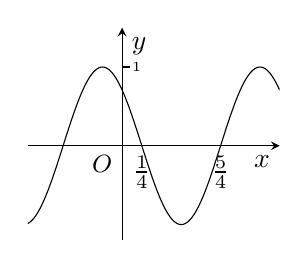
\begin{tikzpicture}
        \node[below left](O) at(0,0) {\small$\bm{O}$};
        \draw(0,1)node[right]{\tiny$1$}--(0.1,1);
        \clip(-1.2,-1.2) rectangle (2,1.5);
        \draw[->,>=stealth](-1.2,0)--(2,0) node[below left] (x){$x$};
        \draw[->,>=stealth](0,-1.2)--(0,1.5) node[below right] (y){$y$};
        \draw[domain=-1.2:2,samples=1000] plot(\x,{cos((pi*(\x)+1/4*pi) r)});
        \node[below] (A)at (0.25,0){$\frac{1}{4}$};
        \node[below] (B)at (1.25,0){$\frac{5}{4}$};
      \end{tikzpicture}
      \end{center}
      \twochx{$ \left(k\pi-\dfrac{1}{4},k\pi+\dfrac{3}{4}\right),k\inZ$}
        {$ \left(2k\pi-\dfrac{1}{4},2k\pi+\dfrac{3}{4}\right),k\inZ$}
        {$ \left(k-\dfrac{1}{4},k+\dfrac{3}{4}\right),k\inZ$}
        {$\left(2k-\dfrac{1}{4},2k+\dfrac{3}{4}\right),k\inZ $}
  \end{exercise}
\section{三角函数模型的简单应用-}
 \fz[12]
$f(x0)=d d$\fz[4]
\section{课后作业}
  \begin{exercise}

  \end{exercise}
\stopexercise
\section{参考答案}
\printanswer

  % \Topic{三角函数单元复习}
  \Teach{}
  \Grade{高一}
  \Name{郑皓天}\FirstTime{20181207}\CurrentTime{20181221}
  % \Name{林叶}\FirstTime{20180908}\CurrentTime{20181125}
  %\Name{1v2}\FirstTime{20181028}\CurrentTime{20181117}
  % \Name{林叶}\FirstTime{20180908}\CurrentTime{20181125}
  % \Name{郭文镔}\FirstTime{20181111}\CurrentTime{20181117}
  % \Name{马灿威}\FirstTime{20181111}\CurrentTime{20181111}
  \newtheorem*{Theorem}{定理}
  \makefront
\vspace{-1.5em}
\startexercise
% \begin{exercise}{\heiti 课前检测}\\
% \end{exercise}
\section{习题}
  % \begin{description}
  %   \item [label]
  % \end{description}
  \begin{exercise}
    \item%高中数学习题解法辞典.pdf 例2-1-8
      已知$\abs{\cos \theta}\leqslant \abs{\sin\theta}$,则$\theta$的取值范围是\tk.
      \begin{answer}
        $\Bigl[k\piup+\dfrac{\piup}4,k\piup+\dfrac{3\piup}4\Bigr],k\in\mathbb{Z}$
      \end{answer}
    \item%高中数学习题解法辞典.pdf 例2-1-19
      已知$\sin\Bigl(\dfrac{\piup}2+2x\Bigr)=-\dfrac12$,则$x=$\tk.
      \begin{answer}
        k\piup\pm\dfrac{\piup}3(k\in\mathbb{Z})
      \end{answer}
    \item%高中数学习题解法辞典.pdf 例2-2-4
      函数$y=\sqrt{25-x^2}+\lg\sin\Bigl(x+\dfrac{\piup}3\Bigr)$的定义域为\tk.
      \begin{answer}
        $\Bigl[-5,-\dfrac{4\piup}3\Bigr)\bigcup\Bigl(-\dfrac{\piup}3,\dfrac{2\piup}3\Bigr)$
      \end{answer}
    \item%《2018天利38套:高考真题单元专题训练(理)ISBN978-7-223-03393-0》专题14三角函数的图像与性质P53p4【2015•全国新课标】【正弦曲线图像】
         %LaTeX-master/sanjiaohanshu/sanjiaohanshu-gaokao.tex 4
      {\kaishu (2015 \textbullet 全国新课标)}
      函数$f(x)=\cos(\omega x+\varphi)$的部分图象如图所示,则$f(x)$的单调递减区间为\xz
      \begin{minipage}[b]{0.8\linewidth}
        \vspace{2.5em}
        \xx{$\Bigl(k\piup-\dfrac{1}{4},k\piup+\dfrac{3}{4}\Bigr),k\in\mathbb{Z}$}
          {$ \Bigl(2k\piup-\dfrac{1}{4},2k\piup+\dfrac{3}{4}\Bigr),k\in\mathbb{Z}$}
          {$ \Bigl(k-\dfrac{1}{4},k+\dfrac{3}{4}\Bigr),k\in\mathbb{Z}$}
          {$\Bigl(2k-\dfrac{1}{4},2k+\dfrac{3}{4}\Bigr),k\in\mathbb{Z} $}
      \end{minipage}\hfill
      \begin{minipage}[h]{0.2\linewidth}
        \vspace{-3cm}
        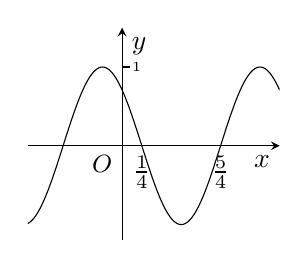
\begin{tikzpicture}
          \node[below left](O) at(0,0) {\small$\bm{O}$};
          \draw(0,1)node[right]{\tiny$1$}--(0.1,1);
          \clip(-1.2,-1.2) rectangle (2,1.5);
          \draw[->,>=stealth](-1.2,0)--(2,0) node[below left] (x){$x$};
          \draw[->,>=stealth](0,-1.2)--(0,1.5) node[below right] (y){$y$};
          \draw[domain=-1.2:2,samples=1000] plot(\x,{cos((pi*(\x)+1/4*pi) r)});
          \node[below] (A)at (0.25,0){$\frac{1}{4}$};
          \node[below] (B)at (1.25,0){$\frac{5}{4}$};
        \end{tikzpicture}
      \end{minipage}
      \begin{answer}
        D
      \end{answer}
    \item%《习题化知识清单》P72知识2-2
      不等式$\tan x>a$在$x\in\Bigl(-\dfrac{\piup}4,\dfrac{\piup}2 \Bigr)$上恒成立,则$a$的取值范围是\xz
      \xx{$(-\infty,-1]$}
        {$(-\infty,-1)$}
        {$(-\infty,1]$}
        {$(-\infty,1]$}
      \begin{answer}
        A
      \end{answer}
    \item%福州三中中学2015-2016学年高一数学第二学期期末检测.docx-9
      (福州三中中学2015-2016学年高一数学第二学期期末检测9)将函数$y=\sin\Bigl(x-\dfrac{\piup}3\Bigr)$的图像上所有点的横坐标伸长到原来的2倍(纵坐标不变),再将所得的图像向左平移$\dfrac{\piup}3$个单位,得到的函数图像对应的解析式是\xz
      \xx{$y=\sin\dfrac x2$}
        {$y=\sin\Bigl(\dfrac x2-\dfrac{\piup}2\Bigr)$}
        {$y=\sin\Bigl(\dfrac{x}2-\dfrac{\piup}6\Bigr)$}
        {$y=\sin\Bigl(2x-\dfrac{\piup}6\Bigr)$}
      \begin{answer}
        C
      \end{answer}
    \item%《习题化知识清单》P73易混清单例
      函数$y=2\sin\Bigl(\dfrac{\piup}3-2x \Bigr)$的单调增区间为\tk.
      \begin{answer}
        $\Bigl[k\piup+\dfrac{5\piup}{12},k\piup+\dfrac{11\piup}{12} \Bigr],k\in\mathbb{Z}$
      \end{answer}
    \item%《习题化知识清单》P72例1
      函数$\dfrac{\sin x+2}{\sin x+1},x\in\Bigl[0,\dfrac{\piup}2\Bigr]$的值域为\tk.
      \begin{answer}
        $\Bigl[\dfrac32,2\Bigr]$
      \end{answer}

    \item%LaTeX-master/sanjiaohanshu/gaokaosection.tex 31
      把函数$ y=\sin 2x $的图象沿$x$轴向左平移$ \dfrac{\piup}{6} $个单位,纵坐标伸长到原来的2倍(横坐标不变)后得到函数$ y=f(x) $的图象,对于函数$ y=f(x) $有以下四个判断:\\
      \ding{192} 该函数的解析式为$ y=2\sin \Bigl(2x+\dfrac{\piup}{6}\Bigr) $;\\
      \ding{193} 该函数图象关于点$ \Bigl(\dfrac{\piup}{3},0\Bigr) $对称;\\
      \ding{194} 该函数在$ \Bigl[0,\dfrac{\piup}{6}\Bigr] $上是增函数;\\
      \ding{195} 若函数$ y=f(x)+a $在$ \Bigl[0,\dfrac{\piup}{2}\Bigr] $上的最小值为$ \sqrt{3},\  $则$ a=2\sqrt{3} .$\\
      其中,正确判断的序号是\tk.
      \begin{answer}
        \circled{2}\circled{4}
      \end{answer}
    \item%福州格致中学2015-2016学年高一数学第二学期期末检测.docx-22
      (福州格致中学2015-2016学年高一数学第二学期期末检测22)已知函数$f(x)=A\sin(\omega x+\varphi)+B (A>0,\omega>0)$的一系列对应值如下表:
      \begin{center}
        \renewcommand{\arraystretch}{1.4}
        \begin{tabular}{|*{8}{c|}}
          \hline
            $x$
            &$\dfrac{\piup}6$
            &$-\dfrac{\piup}3$
            &$-\dfrac{5\piup}6$
            &$-\dfrac{4\piup}3$
            &$-\dfrac{11\piup}6$
            &$-\dfrac{7\piup}3$
            &$-\dfrac{17\piup}6$\\
          \hline
            $y$
            &$-1$
            &$1$
            &$3$
            &$1$
            &$-1$
            &$1$
            &$3$\\
          \hline
        \end{tabular}\\
      \end{center}
      (1)根据表格提供的数据求函数$f(x)$的一个解析式;\\
      (2)根据(1)的结果:\\
      \;(i)当$x\in\Bigl[0,\dfrac{\piup}3\Bigr]$时,方程$f(3x)=m$恰有两个不同的解,求实数$m$的取值范围;\\
      \;(ii)若是$\alpha,\beta$是锐角三角形的两个内角,试比较$f(\sin \alpha)$与$f(\cos \beta)$的大小.
      \begin{answer}
        (1)$f(x)=2\sin\Bigl(x-\dfrac{\piup}3\Bigr)+1$;(2)(i)$[\sqrt{3}+1,3)$;(ii)易得$f(x)$在$[-\dfrac{\piup}6,\dfrac{5\piup}6]$上单调递增,故$f(x)$在$[0,1]$上单调递增;又$0<\dfrac{\piup}2-\beta<\alpha<\dfrac{\piup}2$,从而$\sin\alpha>\sin(\dfrac{\piup}2-\beta)=\cos\beta$,于是$f(\sin \alpha)>f(\cos \beta)$
      \end{answer}
    \vspace{6.5cm}
    \item%高中数学习题解法辞典.pdf 例2-2-9
      已知函数$y=f(x)$的定义域为$\mathbb{R}$,若$f(x+2)=-f(x)$,且当$-1\leqslant x\leqslant 1$时,$f(x)=x$,求证:\\
      (1)函数$y=f(x)$是最小正周期为4的周期函数;\\
      (2)函数$y=f(x)$是奇函数;\\
      (3)当$x\in[4k-1,4k+1](k\in\mathbb{Z})$时,$y=f(x)$是增函数;当$x\in[4k+1,4k+3](k\in\mathbb{Z})$时,$y=f(x)$是减函数.
      \begin{answer}
        (1)(提示:易证4为函数的一个周期;再用反证法证明4是最小正周期:设最小正周期$T$,且$0<T<4$,则$f(T)=f(0)=0$.分类讨论$0<T\leqslant 1$时,$1<T\leqslant 3$时,$3<T<4$时,三种情况都将推出矛盾,于是得证)
        (2)任取$x\inR$,$x$可表示为$x=2k+x'$,其中$-1\leqslant x'\leqslant 1$,$k\inZ$.于是由$f(x+2)=-f(x)$及$y=f(x)$的周期性可得:
        \[f(x)=f(2k+x')=
          \begin{cases}
            -f(x')=-x'\quad(k\text{为奇数})\\
            f(x')=x'\quad(k\text{为偶数})
          \end{cases}
        \]
        注意到$-1\leqslant x'\leqslant 1$,$-1\leqslant -x'\leqslant 1$,又有
        \[f(-x)=f(-2k-x')=
          \begin{cases}
            -f(-x')=x'\quad(k\text{为奇数})\\
            f(-x')=x'\quad(k\text{为偶数})
          \end{cases}
        \]
        综上所述,无论$k$为奇数或偶数,对于$x\inR$,总有$f(-x)=-f(x)$,故$y=f(x)$是奇函数.
        (3)(提示:利用$f(x)=f(4k+x')=f(x')=x'$,其中$-1\leqslant x'\leqslant 1$,$k\inZ$.)
      \end{answer}
  \end{exercise}

\newpage
\section{课后作业}
  \begin{exercise}
    \item%高中数学习题解法辞典.pdf 2-1-74
      已知$1+\sin^2x=\cos x$,则$x=$\tk.
      \begin{answer}
        $2k\piup(k\in\mathbb{Z})$
      \end{answer}
    \item%《习题化知识清单》P72方法2-1
      函数$\abs{\sin x}$的一个单调区间是\xz
      \xx{$\Bigl(\dfrac{\piup}2,\piup\Bigr)$}
        {$\Bigl(\piup,2\piup\Bigr)$}
        {$\Bigl(\piup,\dfrac{3\piup}2\Bigr)$}
        {$\Bigl(0,\piup\Bigr)$}
      \begin{answer}
        C
      \end{answer}
    \item%LaTeX-master/sanjiaohanshu/gaokaosection.tex 13
       已知函数$f(x)=\Bigg\{\begin{aligned}
      \sin(x+a),x\le 0\\\cos (x+b),x>0
      \end{aligned}$是偶函数,则下列结论可能成立的是\xz
       \xx{$ a=\dfrac{\piup}{4},b=-\dfrac{\piup}{4}$}
        {$ a=\dfrac{2\piup}{3},b=\dfrac{\piup}{6}$}
        {$a=\dfrac{\piup}{3},b=\dfrac{\piup}{6} $}
        {$ a=\dfrac{5\piup}{6},b=\dfrac{2\piup}{3}$}
      \begin{answer}
        C
      \end{answer}
    \item%《习题化知识清单》P77单元检测10
      定义在$\mathbb{R}$上的偶函数$f(x)$满足$f(x+1)=-\dfrac2{f(x)}(f(x)\neq0)$,且在区间$(2013,2014)$上单调递增.已知$\alpha,\beta$是锐角三角形的两个内角,则$f(\sin\alpha),f(\cos\beta)$的大小关系是\xz
      \xx{$f(\sin\alpha)<f(\cos\beta)$}
        {$f(\sin\alpha)>f(\cos\beta)$}
        {$f(\sin\alpha)=f(\cos\beta)$}
        {以上情况均有可能}
    \item%《习题化知识清单》P72知识3-3
      若函数$y=2\cos(2x+\varphi)$是偶函数,且在$\Bigl(0,\dfrac{\piup}4\Bigr)$上是增函数,则实数$\varphi$可能是\xz
      \xx{$-\dfrac{\piup}2$}
        {0}
        {{$\dfrac{\piup}2$}}
        {$\piup$}
      \begin{answer}
        D
      \end{answer}
    \item
      比较$\sin 3$,$\cos 3$,$\tan 0.8$的大小关系为\tk.
      \begin{answer}
        $\tan 0.8>\sin 3>\cos 3$
      \end{answer}
    \item%LaTeX-master/sanjiaohanshu/gaokaosection.tex 26
      已知函数$f(x)=\sin (2x+\varphi)$,若$    f\Bigl(\dfrac{\piup}{12}\Bigr)-f\Bigl(-\dfrac{5\piup}{12}\Bigr)=2 $,则函数$f(x)$的单调增区间为\tk.
      \begin{answer}
        $\Bigl[k\piup-\dfrac{5\piup}{12},k\piup+\dfrac{\piup}{12}\Bigr],k\in\mathbb{Z}$
      \end{answer}
    \item%函数y=Asin(ωx+φ)的图象及简单应用P11.9
      若$f(x)=\cos\Bigl(2x+\dfrac{\piup}3+\varphi\Bigr)$$(\abs{\varphi}<\dfrac{\piup}2)$是奇函数,则$\varphi=$\tk.
      \begin{answer}
        $\dfrac{\piup}6$
      \end{answer}
    \item%《习题化知识清单》P77单元检测12
      设$\omega>0$,若函数$f(x)=2\sin \omega x(\omega>0)$在区间$\Bigl[-\dfrac{\piup}3,\dfrac{\piup}4 \Bigr]$上单调递增,则$\omega$取值范围是\tk.
      \begin{answer}
        $\Bigl(0,\dfrac32\Bigr]$
      \end{answer}
    \item%高中数学习题解法辞典.pdf 例2-2-1
      已知函数$f(x)=A\sin(\omega x+\varphi)(A,\omega,\varphi\text{为常数},\omega>0)$的图像上相邻两个最高点的坐标分别是$\Bigl(\dfrac{\piup}{12},2\Bigr)$,$\Bigl(\dfrac{13\piup}{12},2\Bigr)$.\\
      (1) 求函数$f(x)$的一个表达式;\\
      (2)画出函数$f(x)$在长度为一个周期的闭区间上的简图;\\
      (3)说明经过怎样的变换,可以由$y=\sin x$的图像得到$y=f(x)$的图像.
      \begin{answer}
        (1)$y=2\sin\Bigl(2x+\dfrac{\piup}3\Bigr)(\varphi=k\piup-\dfrac{2\piup}3$即可);(2)略;(3)将$y=\sin x$图像上所有点向左平移$\dfrac{\piup}3$个单位得到$y=\sin \Bigl(x+\dfrac{\piup}3\Bigr)$的图像;再把$y=\sin \Bigl(x+\dfrac{\piup}3\Bigr)$的图像上所有点的横坐标缩短到原来的$\dfrac12$(纵坐标不变),得到$y=\sin \Bigl(2x+\dfrac{\piup}3\Bigr)$的图像;最后把$y=\sin \Bigl(2x+\dfrac{\piup}3\Bigr)$的图像上所有点的纵坐标伸长到原来的2倍(横坐标不变),即可得到函数$y=f(x)$的图像.
      \end{answer}
    \vspace{6cm}
    \item%函数y=Asin(ωx+φ)的图象及简单应用P11.14
      已知曲线$y=A\sin(\omega x+\varphi)$$(A>0,\omega>0,\abs{\varphi}\leqslant\dfrac{\piup}2)$上最高点为$(2,\sqrt{2})$,该最高点与相邻的最低点间的曲线与$x$轴交于点$(6,0)$.\\
      (1)该函数的解析式;\\
      (2)该函数在$x\in[-6,0]$上的值域.
      \begin{answer}
        (1)$y=\sqrt{2}\sin\Bigl(\dfrac{\piup}8x+\dfrac{\piup}4\Bigr)$;
        (2)$[-\sqrt{2},0]$
      \end{answer}
    \vspace{5cm}
    \item%高中数学习题解法辞典.pdf 2-2-44
      已知函数$f(x)=2\sin\Bigl(\omega x+\dfrac{\piup}6\Bigr)+1(\omega>0)$,\\
      (1)求$f(x)$的最大值$M$,最小值$m$以及最小正周期$T$;\\
      (2)试求最小正整数$\omega$,使得自变量$x$在任意两个整数间(包括整数本身)变化时,函数$f(x)$至少有一个值是$M$,另一个值是$m$.
      \begin{answer}
        (1)$M=3,m=-1,T=\dfrac{2\piup}{\omega}$;(2)$\dfrac{2\piup}{\omega}\leqslant 1$,$\omega=7$(周期为无理数,由“无理数无法表示为两整数之比”这一事实可得任一区间$[k,k+1]$,$k\inZ$内函数图像均不相同.由此,半周期必须不小于1才能满足题意)
      \end{answer}
    \vspace{6cm}
    \item%高中数学习题解法辞典.pdf 2-2-45
      求证:(1)$f(x)=\sin x\cos x$的最小正周期为$\piup$;\\
      (2)若函数$y=f(x)(x\in\mathbb{R})$的最小正周期为$T$,则$f(kx)(k>0)$的最小正周期为$\dfrac{T}k$.
      \begin{answer}
        (1)(提示:若$0<T<\piup$,令$x=0$,得$T=\dfrac{\piup}2$,不符);(2)(提示:$f\biggl[k\Bigl(x+\dfrac{T}k\Bigr)\biggr]=f(kx+T)=f(kx)$)
      \end{answer}
  \end{exercise}
\stopexercise

\newpage
\section{部分参考答案}
\begin{multicols}{2}
  \printanswer
\end{multicols}

  % \Topic{向量基本概念与线性运算}
  \Teach{向量共线定理及其运用}
  \Grade{高一}
  %\Name{1v2}\FirstTime{20181028}\CurrentTime{20181117}
  % \Name{林叶}\FirstTime{20180908}\CurrentTime{20181125}
  % \Name{郭文镔}\FirstTime{20181111}\CurrentTime{20181117}
  % \Name{马灿威}\FirstTime{20181111}\CurrentTime{20181111}
  \newtheorem*{Theorem}{定理}
  \makefront
\vspace{-1.5em}
\startexercise
\section{向量的基本相关概念}
  \begin{description}
    \item[有向线段]带有方向的线段.用$\vv{AB}$表示;线段AB的长度也叫做有向线段$\vv{AB}$的长度,记作$\abs{\vv{AB}}$.\par
      {\kaishu 有向线段包含三要素:{\textbf 起点、方向、长度}}
    \item[向量] 既有大小,又有方向的量,用$ \vv{a},~\vv{AB},~\bm{a} $表示;向量的大小叫做向量的长度或向量的模,用$ \abs{\bm{a}} $表示.\par
      \begin{itemize}[leftmargin=*]
        \kaishu
        \item 不同于有向线段,平面向量是自由向量(无源向量);
        \item 只有大小,没有方向的量称为数量;(物理学中通常称数量为标量,并把向量称为矢量)
      \end{itemize}
    \item[零向量] 长度为零的向量,其方向是任意的,记作$ \vv{0} $或$ \bm{0} $;
    \item[相等向量] 长度相等且方向相同的向量;\par
      {\kaishu 两个向量只能相等或者不相等,不能比较大小.}
    \item[相反向量] 长度相等且方向相反的向量\par
      {\kaishu 规定:$\bm{0}$的相反向量为$\bm{0}$}
    \item[单位向量] 长度等于一个单位长度的向量;\par
      {\kaishu 与向量$\bm a$方向相同的向量通常记为$\hat{\bm a}(=\dfrac{\bm a}{\abs{\bm a}})$}(一般手写为$\hat a$即可).
    \item[平行向量(共线向量)]方向相同或相反的非零向量叫做平行向量或共线向量;规定零向量与任一向量平行共线.
      向量$\bm{a}$、$\bm{b}$平行记作$\bm{a}\varparallel \bm{b}$.\par
      {\kaishu 向量平行不具有传递性}
    \item[向量的夹角] 已知两个非零向量$\bm a$和$\bm b$,如图,做$\vv{OA}=\bm a$,$\vv{OB}=\bm b$,
      则$\angle{AOB}=\theta$叫做向量$\bm a$和$\bm b$的夹角.记作$\vangle{\bm a}{\bm b}$或$\vangle{\bm b}{\bm a}$.\par
      \begin{minipage}[b]{0.8\linewidth}
        \begin{itemize}
          \kaishu
          \item 向量夹角的取值范围:$[0,\piup]$ ;
          \item 当$\theta=0\degree$时,向量$\bm a,\bm b$共线且同向;
          \item 当$\theta=90\degree$时,向量$\bm a,\bm b$相互垂直,记作$\bm a\perp \bm b$;
          \item 当$\theta=180\degree$时,向量$\bm a,\bm b$共线且反向.
        \end{itemize}
      \end{minipage}\hfill
      \begin{minipage}[h]{0.2\linewidth}
        \vspace{-3.5cm}
        \begin{tikzpicture}[scale=1.5]
          \coordinate[lable=below:$O$](O) at (0,0);
          \coordinate[label=below:$A$](A) at (2,0);
          \coordinate[label=left:$B$](B) at(1,2);
          \draw[->,>=latex] (O)--(A)node[midway ,below](a){\small$\bm{a}$};
          \draw[->,>=latex] (O)--(B)node[midway, left](b){\small$\bm{b}$};
          \path (A)--(O)--(B) pic [draw,"$\theta$",angle eccentricity=1.5] {angle=A--O--B};
        \end{tikzpicture}
      \end{minipage}
  \end{description}
  \begin{exercise}{\textbf{基础测试}}
    \item
      判断下列结论是否正确(请在括号中打“\checkmark”或“\XSolidBrush”)\\
      (1)向量与有向线段是一样的,因此可以用有向线段来表示向量.(  )\\
      (2)$\abs{\bm{a}}$与$\abs{\bm{b}}$是否相等与$\bm{a}$,$\bm{b}$的方向无关.(  )\\
      (3)若$\bm{a}\varparallel\bm{b}$,$\bm{b}\varparallel\bm{c}$,则$\bm{a}\varparallel\bm{c}$.(  )\\
      (4)若向量$\vv{AB}$与向量$\vv{CD}$是共线向量,则$A,B,C,D$四点在一条直线上.(  )\\
      (5)若向量$\vv{AB}$与向量$\vv{CD}$平行,则直线$AB$与$CD$平行.(  )\\
      (6)若向量$\bm a$与任一向量$\bm b$平行,则$\bm a=\bm 0$.(  )\\
      (7)若两个向量共线,则其方向必定相同或相反.(  )
      \begin{answer}
        (2)(5)正确
      \end{answer}
    \item
      有下列命题:
      \circled{1}两个相等向量,它们的起点相同,终点也相同;
      \circled{2}若$\abs{\bm{a}}=\abs{\bm{b}}$,则$\bm{a}=\bm{b}$;
      \circled{3}若$\abs{\vv{AB}}=\abs{\vv{CD}}$,则四边形$ABCD$是平行四边形;
      \circled{4}若$\bm{m}=\bm{n}$,$\bm{n}=\bm{k}$,则$\bm{m}=\bm{k}$;
      \circled{5}位移、速率、重力加速度都是向量;
      \circled{6}共线的向量,若起点不同,则终点一定不同.其中,错误的个数是\xz
      \xx{2}{3}{4}{5}
    \item
      正方形$ABCD$中,向量$\vv{AC}$与$\vv{BC}$的夹角为\tk,向量$\vv{AC}$与$\vv{CD}$的夹角为\tk.
    \item
      在平面内,若将所有单位向量的起点平移到同一点,则它们的终点构成的图形为\tk.
  \end{exercise}
\section{向量的线性运算}
  向量的线性运算包括向量的加、减、数乘运算.
  \subsection{加法}
    \begin{description}
      \item[定义] 两个向量和的运算;
      \item[法则] 平行四边形法则或三角形法则
        \begin{center}
        \begin{tikzpicture}
          \coordinate(O) at (0,0);
          \coordinate(A) at (2,0);
          \coordinate(B) at(1,2);
          \coordinate(C) at ($(A)+(B)$);
          \draw[->,>=latex] (O)--(A)node[midway,below](a){\small$\bm{a}$};
          \draw[->,>=latex] (O)--(C)node[midway,above,sloped](c){\small$\bm{a}+\bm{b}$};
          \draw[->,>=latex] (A)--(C)node[midway, below](b){\small$\bm{b}$};
          \begin{scope}[xshift=4cm]
            \coordinate(O) at (0,0);
            \coordinate(A) at (2,0);
            \coordinate(B) at(1,2);
            \coordinate(C) at ($(A)+(B)$);
            \draw[->,>=latex] (O)--(A)node[midway ,below](a){\small$\bm{a}$};
            \draw[->,>=latex] (O)--(C)node[midway ,below,sloped](c){\small$\bm{a}+\bm{b}$};
            \draw[->,>=latex] (O)--(B)node[midway, left](b){\small$\bm{b}$};
            \draw[dashed](B)--(C);
            \draw[dashed](A)--(C);
          \end{scope}
        \end{tikzpicture}
        \end{center}
        {\kaishu 对于零向量与任一向量$\bm{a}$,规定$$\bm{a}+\bm{0}=\bm{0}+\bm{a}=\bm{a}$$}\par
        由三角形法则,可得向量不等式(有时称作“三角形不等式”):
        \[\bigm|{\abs{\bm{a}}-\abs{\bm{b}}\bigm|}\leqslant \abs{\bm{a}+\bm{b}}\leqslant \abs{\bm{a}}+\abs{\bm{b}}\]
        若$\bm a$和$\bm b$为非零向量,则:当$\bm a$与$\bm b$反向时, 左边等式成立;当$\bm a$与$\bm b$同向时, 右边等式成立;\par
      \item[运算律]
        \begin{itemize}%[leftmargin=*]
          \item 交换律:$\bm{a}+\bm{b}=\bm{b}+\bm{a}$\
          \item 结合律:$(\bm{a}+\bm{b})+\bm{c}=\bm{a}+(\bm{b}+\bm{c})$
        \end{itemize}
    \end{description}
  \subsection{减法}
    \begin{description}
      \item[定义]减去一个向量相当于加上这个向量的相反向量,即$$\bm{a}-\bm{b}=\bm{a}+(\bm{-b})$$
      \item[运算法则]三角形法则、平行四边形法则.%$\vv{AB}-\vv{AC}=\vv{CB}$.
      \begin{center}
      \begin{tikzpicture}
        \coordinate(O) at (0,0);
        \coordinate(A) at (2,0);
        \coordinate(B) at(1.5,1.5);
        \draw[->,>=latex] (O)--(A)node[midway,below](a){\small$\bm{b}$};
        \draw[->,>=latex] (O)--(B)node[midway, left](a){\small$\bm{a}$};
        \draw[->,>=latex](A)--(B)node[midway, above,sloped](a){\small$\bm{a}-\bm{b}$};
        \begin{scope}[xshift=6cm]
          \coordinate(O) at (0,0);
          \coordinate(B) at (2,0);
          \coordinate(A) at(1.5,1.5);
          \coordinate(B1) at (-2,0);
          \coordinate(C)at($(B1)+(A)$);
          \draw[->,>=latex] (O)--(B)node[midway,below](a){\small$\bm{b}$};
          \draw[->,>=latex] (O)--(A)node[midway, left](a){\small$\bm{a}$};
          \draw[->,>=latex](B)--(A)node[midway, above,sloped](a){\small$\bm{a}-\bm{b}$};
          \draw[->,>=latex](O)--(B1)node[midway,below](b1){\small$\bm{-b}$};
          \draw[->,>=latex](O)--(C)node[midway,below,sloped](b1){\small$\bm{a-b}$};
          \draw[dashed] (B1)--(C) (A)--(C);
        \end{scope}
      \end{tikzpicture}
      \end{center}
      {\kaishu
        对于任意一点$P$,$\vv{AB}=\vv{PB}-\vv{PA}$,
      }
    \end{description}
  \subsection{数乘}
    \begin{description}
      \item[定义] 求实数$ \lambda $与向量$\bm{a}$的积是一个向量,记作$\lambda\bm{a}$,长度与方向由以下法则规定:
      \item[法则]
        \begin{enumerate}[label=\arabic*)]
          \item $\abs{\lambda \bm{a}}=\abs{\lambda}\abs{\bm{a}} $;
          \item
            \begin{itemize}
              \item 当$ \lambda>0 $时,$ \lambda\bm{a} $的方向与$\bm{a}$的方向相同;
              \item 当$ \lambda<0 $时,$ \lambda\bm{a} $的方向与$\bm{a}$的方向相反;
              \item 当$ \lambda=0 $时,$ \lambda\bm{a}=\bm 0 $.
            \end{itemize}
        \end{enumerate}
      \item[运算律]
        设$\lambda,\mu\in\mathbb{R}$,则:\par
        \begin{itemize}
            \item $\lambda(\mu\bm{a})=(\lambda\mu)\bm{a}$;
            \item $(\lambda+\mu)\bm{a}=\lambda\bm{a}+\mu\bm{a}$;
            \item $\lambda(\bm{a}+\bm{b})=\lambda\bm{a}+\lambda\bm{b}$.
        \end{itemize}
      对于任意向量$\bm a,\bm b$以及任意实数$\lambda$,$\mu_1$,$\mu_2$,恒有:
      \[\lambda({\mu_1\bm a}\pm{\mu_2\bm b})={\lambda\mu_1\bm a}\pm{\lambda\mu_2\bm b}\]
    \end{description}
    \begin{Theorem}[向量共线定理]
      向量$\bm{a}~(\bm{a}\ne\bm{0})$与向量$\bm{b}$共线,当且仅当存在唯一的实数$ \lambda $,使得$\bm{b}=\lambda\bm{a}$.
    \end{Theorem}
    {\kaishu
     证明三点共线的方法:\circled{1}$\vv{AB}=\lambda\vv{AC}$,则$A$,$B$,$C$三点共线;\circled{2}$\vv{OA}=\lambda\vv{OB}+\mu\vv{OC}$,若$\lambda+\mu=1$,则$A$,$B$,$C$三点共线.
    }
  \clearpage
  \begin{exercise}{\textbf{基础测试}}
    \item
      如图,$\vv{AB}+\vv{BC}-\vv{AD}$等于\xz
      \begin{minipage}[b]{0.7\linewidth}
      	\xx{$\vv{AD}$}{$\vv{DC}$}{$\vv{DB}$}{$\vv{AB}$}
      \end{minipage}\hfill
      \begin{minipage}[h]{0.3\linewidth}
        \begin{tikzpicture}
          \coordinate[label=left:$B$](B)at(0,0);
          \coordinate[label=right:$C$](C)at(3,0);
          \coordinate[label=above:$A$](A)at(1.5,2);
          \coordinate[label=below:$D$](D)at($(B)!0.4!(C)$);
          \draw (A)--(B)--(C)--cycle;
          \draw (A)--(D);
        \end{tikzpicture}
      \end{minipage}
      \begin{answer}
        B
      \end{answer}
    \item%1平面向量的基本概念.pdf P10-训练1
      判断下列结论是否正确(请在括号中打“\checkmark”或“\XSolidBrush”)\\
      (1)若向量$\bm b$与向量$\bm{a}$共线,则存在唯一的实数$ \lambda $,使得$\bm{b}=\lambda\bm{a}$.(\hspace{2em})\\
      (2)若$\bm{b}=\lambda\bm{a}$,则$\bm a$与$\bm b$共线.(\hspace{2em})\\
      (3)若$\lambda\bm a=\bm 0$,则$\bm a=\bm 0$.(\hspace{2em})\\
    \item
      如图所示,在五边形$ABCDE$中,若四边形$ACDE$是平行四边形,且$\vv{AB}=\bm{a}$,$\vv{AC}=\bm{b}$,$\vv{AE}=\bm{c}$,试用向量$\bm a$,$\bm b$,$\bm c$表示向量$\vv{BD}$,$\vv{BC}$,$\vv{BE}$,$\vv{CD}$及$\vv{CE}$.
      \begin{flushright}
        \begin{tikzpicture}
          \coordinate[label=left:$D$](D)at(0,0);
          \coordinate[label=right:$E$](E)at(3,0);
          \coordinate[label=above:$C$](C)at(1,1.5);
          \coordinate[label=below:$A$](A)at($(C)+(E)$);
          \coordinate[label=below:$B$](B)at(3.5,2.5);
          \draw (A)--(B)--(C)--(D)--(E) --cycle;
          \draw (B)--(D) (B)--(E) (C)--(E);
          \draw[->,>=latex] (A)--(B);
          \draw[->,>=latex] (A)--(C);
          \draw[->,>=latex] (A)--(E);
        \end{tikzpicture}
      \end{flushright}
      \begin{answer}
        $\vv{BD}=-\bm a+\bm c+\bm b$;$\vv{BC}=\bm b-\bm a$;$\vv{BE}=\bm a-\bm a$;$\vv{CD}=\bm c$;$\vv{CE}=\bm c-\bm b$.
      \end{answer}
    \item
      \begin{enumerate}[label=\arabic*)]
        \item $3(6\bm{a}+\bm{b})-9(\bm{a}+\dfrac13\bm{b})=$\tk;
        \item 若$2(\bm{y}-\dfrac13\bm{a})-\dfrac12(\bm c+\bm b-3\bm y)+\bm b=0$其中$\bm a$,$\bm b$,$\bm c$为已知向量,则未知向量$\bm y=$\tk.
        \item 若$\bm a=\bm b+\bm c$,化简$3(\bm a+2\bm b)-2(3\bm b+\bm c)-2(\bm a+\bm b)=$\tk.
      \end{enumerate}
      \begin{answer}
        (1)$9\bm a$;(2)$\dfrac4{21}\bm a-\dfrac17\bm b+\dfrac17\bm c$;$-\bm a$.
      \end{answer}
    \item%《习题化知识清单》P81知识4-3【向量共线】
      已知向量$\bm a$、$\bm b$,且$\vv{AB}=\bm a+2\bm b$,$\vv{BC}=-5\bm a+6\bm b$,$\vv{CD}=7\bm a-2\bm b$,则一定共线的三点是\xz
      \xx{$A$、$B$、$D$}
        {$A$、$B$、$C$}
        {$B$、$C$、$D$}
        {$A$、$C$、$D$}
      \begin{answer}
        A
      \end{answer}
    \item%《习题化知识清单》P81知识4-4【向量线性运算、向量共线】
      已知向量$\bm a=\bm e_1+2\bm e_2$,$\bm b=2\bm e_1-\bm e_2$,则$\bm a+2\bm b$与$2\bm a-\bm b$\xz
      \xx{一定共线}
        {一定不共线}
        {当且仅当$\bm e_1$与$\bm e_2$共线时共线}
        {当且仅当$\bm e_1=\bm e_2$时共线}
      \begin{answer}
        C
      \end{answer}
  \end{exercise}
\newpage
\section{习题}
  \begin{exercise}
    \item%1平面向量的基本概念.pdf P3训练3
      一辆汽车从$A $点出发向西行驶了100 km 到达$B $点,然后又改变方向向西偏北$50\degree$走了200 km到达$C$ 点,最后又改变方向,向东行驶了100 km 到达$D$ 点.\\
      (1)作出向量$\vv{AB}$,$\vv{BC}$,$\vv{CD}$;\\
      (2)求$\abs{\vv{AD}}$.\\
    \vspace{4cm}\\
    \begin{minipage}[b]{0.65\linewidth}
    \item%LaTeX-master/xiangliang/xiangliangsorting.tex P10-p48
      在$\triangle ABC$中,点$ M$,$N $满足$ \vv{AM}=2\vv{MC}$,$\vv{BN}=\vv{NC}$.若$\vv{MN}=x\vv{AB}+y\vv{AC}$,则$ x= $\tk;$ y= ~$ \tk.
      \begin{answer}
        $x=\dfrac12$;$y=-\dfrac16$
      \end{answer}
    \end{minipage}
    \begin{minipage}[htbp!]{0.3\linewidth}
      \begin{center}
      \begin{tikzpicture}
        \draw(0,0)node[below](B){\small$B$}--(1,0)node[below](N){\small$N$}--(2,0)node[below](C){\small$C$};
        \draw (0,0)--(1.1,2.1)node[above](A){\small$A$}--(2,0);
        \draw (1,0)--(1.1,2.1);
        \draw(1,0)--($(1.1,2.1)!0.7!(2,0)$)node[right](M){\small$M$};
      \end{tikzpicture}
      \end{center}
    \end{minipage}
    \item
      (2018届贵州遵义航天高级中学一模)如图所示,向量$\vv{OA}=\bm{a}$,$\vv{OB}=\bm{b}$,$\vv{OC}=\bm{c}$,$A$,$B$,$C$在一条直线上,且$\vv{AC}=3\vv{BC}$,则\xz
      \begin{minipage}[b]{0.7\linewidth}
        \xx{$\bm{c}=\dfrac32\bm{b}-\dfrac12\bm{a}$}
          {$\bm{c}=\dfrac32\bm{a}-\dfrac12\bm{b}$}
          {$\bm{c}=-\bm{a}+2\bm{b}$}
          {$\bm{c}=\bm{a}+2\bm{b}$}
      \end{minipage}\hfill
      \begin{minipage}[htbp!]{0.3\linewidth}
        \begin{center}
        \begin{tikzpicture}
          \coordinate[label=left:$O$](O)at(0,0);
          \coordinate[label=right:$C$](C)at(3,0);
          \coordinate[label=left:$A$](A)at(-1,2.5);
          \coordinate[label=right:$B$](B)at($(A)!0.66!(C)$);
          \draw (A)--(B)--(C)--cycle;
          \draw[->,>=latex] (O)--(C);
          \draw[->,>=latex] (O)--(A);
          \draw[->,>=latex] (O)--(B);
        \end{tikzpicture}
        \end{center}
      \end{minipage}
      \begin{answer}
        A
      \end{answer}
    \item
      设向量$\bm a$,$\bm b$不共线,向量$\lambda\bm a+\bm b$与$\bm a+2\bm b$共线,则实数$\lambda=$\tk.
      \begin{answer}
        $\dfrac12$
      \end{answer}
    \vspace{2em}
    \item
      如图,在$\triangle ABC$中,$D$,$E$为边$AB$的两个三等分点,$\vv{CA}=3\bm a$,$\vv{CB}=2\bm b$,求$\vv{CD}$,$\vv{CE}$(用$\bm a$,$\bm b$表示).
      \begin{flushright}
        \begin{tikzpicture}
          \coordinate[label=left:$B$](B)at(0,0);
          \coordinate[label=right:$C$](C)at(2.5,0);
          \coordinate[label=above:$A$](A)at(3,3);
          \coordinate[label=above:$E$](E)at($(B)!0.33!(A)$);
          \coordinate[label=above:$D$](D)at($(B)!0.66!(A)$);
          \draw (A)--(B)--(C) --cycle;
          \draw (C)--(D) (C)--(E);
          \draw[->,>=latex] (C)--(A);
          \draw[->,>=latex] (C)--(B);
        \end{tikzpicture}
      \end{flushright}
      \begin{answer}
        $\vv{CD}=2\bm a+\dfrac23\bm b$;$\vv{CE}=\bm a+\dfrac43\bm b$
      \end{answer}
    \item%1平面向量的基本概念.pdf P10例2
      设$\bm a$,$\bm b$是不共线的两个非零向量.\\
      (1)若$\vv{OA}=2\bm a-\bm b$,$\vv{OB}=3\bm a+\bm b$,$\vv{OC}=\bm a-3\bm b$,求证:$A$,$B$,$C$三点共线;\\
      (2)若$8\bm a+k\bm b$与$k\bm a+\2\bm b$共线,求实数$k$的值;\\
      (3)若$\vv{OM}=m\bm a$,$\vv{ON}=n\bm b$,$\vv{OP}=\alpha\bm a+\beta\bm b$,其中$m$,$n$,$\alpha$,$\beta$均为实数,且$m,n\neq 0$,若$M$,$P$,$N$三点共线,求证:$\dfrac{\alpha}m+\dfrac{\beta}n=1$
      \begin{answer}
        (1)$\because \vv{AB}=\bm a+2\bm b$,$\vv{CB}=2\bm a+4\bm b$;$\therefore \vv{CB}=2\vv{AB}$;
        (2)$k=2\sqrt2$;
      \end{answer}
      \vspace{5cm}
    \item
      设点$G$为$\triangle ABC$重心,$D$,$E$,$F$分别为各边中点.试用向量证明:$AG=\dfrac23 AD$.
      \begin{flushright}
        \begin{tikzpicture}
          \coordinate[label=left:$B$](B)at(0,0);
          \coordinate[label=right:$C$](C)at(3,0);
          \coordinate[label=above:$A$](A)at(2,2);
          \coordinate[label=below:$D$](D)at($(B)!0.5!(C)$);
          \coordinate[label=right:$E$](E)at($(A)!0.5!(C)$);
          \coordinate[label=above:$F$](F)at($(B)!0.5!(A)$);
          \coordinate[label=above:$G$](G)at($(D)!0.33!(A)$);
          \draw (A)--(B)--(C) --cycle;
          \draw (A)--(D) (B)--(E) (C)--(F);
        \end{tikzpicture}
      \end{flushright}
    \vspace{2cm}
  \end{exercise}
\clearpage
\section{课后作业}
  \begin{exercise}
    \item%1平面向量的基本概念.pdf P2-训练1
      判断下列结论是否正确(请在括号中打“\checkmark”或“\XSolidBrush”)\\
      (1)向量就是有向线段.(  )\\
      (2)如果$\abs{\vv{AB}}>\abs{\vv{CD}}$,那么$\vv{AB}>\vv{CD}$.(  )\\
      (3)力、速度和质量都是向量.(  )\\
      (4)若$\bm a$,$\bm b$都是单位向量,则$\bm a=\bm b$.(  )\\
      (5)若$\bm a=\bm b$,且$\bm a$与$\bm b$的起点相同,则终点也相同.(  )\\
      (6)零向量的大小为0,没有方向.(  )
      \begin{answer}
        (5)正确,其余皆误.
      \end{answer}
    \item
      给出下列命题:
      \ding{192}两个具有公共终点的向量,一定是共线向量;
      \ding{193}两个向量不能比较大小,但它们的模能比较大小;
      \ding{194}$\lambda\bm{a}=\bm{0}$($\lambda$为实数),则$\lambda$必为零;
      \ding{195}$\lambda$,$\mu$为实数,若$\lambda\bm{a}=\mu\bm{b}$,则$\bm{a}$与$\bm{b}$共线.
      其中正确的命题的个数为\xz
      \xx{1}{2}{3}{4}
      \begin{answer}
        A
      \end{answer}
    \item
      (2018·安徽淮北第一中学最后一卷)设$\bm{a}$,$\bm{b}$都是非零向量,下列四个条件,使$\dfrac{\bm{a}}{\abs{\bm{a}}}=\dfrac{\bm{b}}{\abs{\bm{b}}}$成立当且仅当\xz
      \xx{$\bm a=\bm b$}
      {$\bm a=2\bm b$}
      {$\bm a\varparallel\bm b$且$\abs{\bm a}=\abs{\bm b}$}
      {$\bm a\varparallel\bm b$且方向相同}
      \begin{answer}
        D
      \end{answer}
    \item
      已知四边形$ABCD$ 是菱形,则下列等式中成立的是\xz
      \xx{$\vv{AB}+\vv{BC}=\vv{CA}$}
        {$\vv{AB}+\vv{AC}=\vv{BC}$}
        {$\vv{AC}+\vv{BA}=\vv{AD}$}
        {$\vv{AC}+\vv{AD}=\vv{DC}$}
      \begin{answer}
        C
      \end{answer}
    \item%1平面向量的基本概念.pdf P13-4
      已知$AM$ 是$\triangle ABC$ 的边$BC$ 上的中线,若$\vv{AB}=\bm a$,$\vv{AC}=\bm b$,则$\vv{AM}$等于\xz
      \xx{$\dfrac12(\bm a-\bm b)$}
        {$-\dfrac12(\bm a-\bm b)$}
        {$\dfrac12(\bm a+\bm b)$}
        {$-\dfrac12(\bm a+\bm b)$}
      \begin{answer}
        C
      \end{answer}
    \item%《习题化知识清单》P81知识4-1【向量共线】
      已知向量$\bm a$、$\bm b$不共线,$\bm c=k\bm a+\bm b({k\in\mathbb{R}})$,$\bm d=\bm a-\bm b$。如果$\bm c\varparallel \bm d$,那么\xz
      \xx{$k=1$且$\bm c$与$\bm d$同向}
        {$k=1$且$\bm c$与$\bm d$反向}
        {$k=-1$且$\bm c$与$\bm d$同向}
        {$k=-1$且$\bm c$与$\bm d$反向}
      \begin{answer}
        D
      \end{answer}
    \item%1平面向量的基本概念.pdf P13-10
      化简:\\
      \circled{1} $\vv{BC}+\vv{AB}$; \hspace{2em} \circled{2} $\vv{DB}+\vv{CD}+\vv{BC}$;\\
      \circled{3} $\vv{AB}-\vv{FD}+\vv{CD}-\vv{CB}+\vv{FA}$;\hspace{2em} \circled{4} $(\vv{AC}+\vv{BO}+\vv{OA})-(\vv{DC}-\vv{DO}-\vv{OB})$;\\
      \begin{answer}
        \circled{1}$\vv{AC}$;\circled{2}$\bm 0$;\circled{3}$\bm 0$;\circled{4}$\bm 0$
      \end{answer}
    \vspace{1.5cm}
    \item%1平面向量的基本概念.pdf P8训练5
      一架飞机从$A$ 地按北偏东$35\degree$的方向飞行800 km 到达$B$ 地接到受伤人员,然后又从$B$ 地按南偏东$55\degree$的方向飞行600 km 送往$C $地医院,求这架飞机飞行的路程及两次位移的和.
      \begin{answer}
        路程1400km,位移1000km.
      \end{answer}
    \vspace{4cm}
    \item
      设点$G$为$\triangle ABC$重心,$D$,$E$,$F$分别为各边中点.\\
      (1)试用向量证明:三角形三条中线共点;
      (2)求$\vv{AD}+\vv{BE}+\vv{CF}$.
      \begin{flushright}
        \begin{tikzpicture}
          \coordinate[label=left:$B$](B)at(0,0);
          \coordinate[label=right:$C$](C)at(3,0);
          \coordinate[label=above:$A$](A)at(2,2);
          \coordinate[label=below:$D$](D)at($(B)!0.5!(C)$);
          \coordinate[label=right:$E$](E)at($(A)!0.5!(C)$);
          \coordinate[label=above:$F$](F)at($(B)!0.5!(A)$);
          \coordinate[label=above:$G$](G)at($(D)!0.33!(A)$);
          \draw (A)--(B)--(C) --cycle;
          \draw (A)--(D) (B)--(E) (C)--(F);
        \end{tikzpicture}
      \end{flushright}
      \vspace{2cm}
    \item
      已知$\vv{OA}=\lambda\vv{OB}+\mu\vv{OC}$($\lambda,\mu\in\mathbb{R}$),若$\lambda+\mu=1$,求证:点$A$,$B$,$C$三点共线.\\
      \vspace{4cm}
    \item
      【定比分点坐标公式】如图,设$P$为$\triangle ABO$边$AB$上一点.设$\vv{OA}=\bm a$,$\vv{OB}=\bm b$\vspace{8pt}\\
      (1)求证:$\vv{OP}=\dfrac{\abs{\vv{PB}}}{\abs{\bm b-\bm a}}\bm a+\dfrac{\abs{\vv{PA}}}{\abs{\bm b-\bm a}}\bm b$;\vspace{8pt}\\
      (2)设$\vv{AP}=\lambda\vv{PB}$,求证:$\vv{OP}=\dfrac{\bm a+\lambda\bm b}{1+\lambda}$
      \begin{flushright}
        \begin{tikzpicture}
          \coordinate[label=left:$O$](O)at(0,0);
          \coordinate[label=right:$A$](A)at(3,0);
          \coordinate[label=above:$B$](B)at(2,2);
          \coordinate[label=right:$P$](P)at($(B)!0.4!(A)$);
          \draw (A)--(B)--(O) --cycle;
          \draw[->,>=latex] (O)--(A);
          \draw[->,>=latex] (O)--(B);
          \draw[->,>=latex] (O)--(P);
        \end{tikzpicture}
      \end{flushright}
  \end{exercise}
\stopexercise
\newpage
\section{部分参考答案}
\printanswer

  % \Topic{平面向量坐标表示,数量积}
  \Teach{向量共线与数量积的坐标表示}
  \Grade{高一}
  % \Name{郑皓天}\FirstTime{20181207}\CurrentTime{20181207}
  % \Name{林叶}\FirstTime{20180908}\CurrentTime{20181125}
  % \Name{1v2}\FirstTime{20181028}\CurrentTime{20181117}
  % \Name{林叶}\FirstTime{20180908}\CurrentTime{20181125}
  % \Name{郭文镔}\FirstTime{20181111}\CurrentTime{20181117}
  % \Name{马灿威}\FirstTime{20181111}\CurrentTime{20181111}
  \newtheorem*{Theorem}{定理}
  \makefront
\vspace{-1.5em}

\startexercise
% \begin{exercise}{\heiti 课前检测}\\
%   表格实例:
%   \begin{center}
%     \renewcommand{\arraystretch}{1.4}
%     \begin{tabular}{|*{8}{c|}}
%       \hline
%         $x$
%         &$-\dfrac{\piup}6$
%         &$-\dfrac{\piup}3$
%         &$-\dfrac{5\piup}6$
%         &$-\dfrac{4\piup}3$
%         &$-\dfrac{11\piup}6$
%         &$-\dfrac{7\piup}3$
%         &$-\dfrac{17\piup}6$\\
%       \hline
%         $y$
%         &$-1$
%         &$1$
%         &$3$
%         &$1$
%         &$-1$
%         &$1$
%         &$3$\\
%       \hline
%     \end{tabular}\\
%   \end{center}
% \end{exercise}

\section{平面向量基本定理及坐标表示}
  \subsection{基底}
    \begin{Theorem}[平面向量基本定理]
      如果$ \bm{e}_1,\bm{e}_2 $是同一平面内的两个\CJKunderdot{不共线}的向量,那么对于这一平面内的任意向量$ \bm{a} $,有且只有一对实数$ \lambda_1,~\lambda_2 $,使$\bm{a}=\lambda_1\bm{e}_1+\lambda_2\bm{e}_2$.\par 其中,不共线的向量$ \bm{e}_1,~\bm{e}_2 $叫做表示这一平面内所有向量的一组\CJKunderdot{基底}.
    \end{Theroem}
    {\kaishu 解决向量问题,需要注意两点:一是向量共线定理,一个是平面向量基本定理.\par
    向量的基底的重要性在于一旦有了基底,你就可以将题目中涉及的所有向量都用基底向量唯一的表示出来(坐标表示就是一组特殊的基底),计算和变形都有了方向,便于寻找和发现关系.如果题目没有明确给出基底,那么就需要自己指定了}
  \subsection{坐标表示}
    在不共线的向量中,垂直是一种重要的情形,把一个向量分解为两个互相垂直的向量,叫做把向量\CJKunderdot{正交分解}.\par
    在平面直角坐标系$xOy$中,分别取与$x$轴、$y$轴方向相同的两个\CJKunderdot{单位向量}$~ \bm{i},~\bm{j} $作为基底.对于平面内的一个向量$ \bm{a} $,由平面向量基本定理可知,有且只有一对实数$ x,~y $使得\[\bm{a}=x\bm{i}+y\bm{j}\]
    这样,平面内的任一向量$ \bm{a} $都可以由$ x,~y $唯一确定,我们把有序数对$ (x,y) $叫做向量$\bm{a}  $的坐标,记作
    \begin{equation}\label{eq:axy}
      \bm{a}=(x,y)
    \end{equation}
    其中$ x $叫做$ \bm{a} $在$x$轴上的坐标,$ y $叫做$ \bm{a} $在$y$轴上的坐标,(\ref{eq:axy})式叫做\textbf{向量的坐标表示}
    \begin{center}
    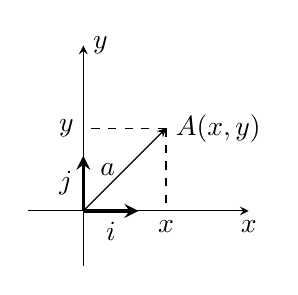
\begin{tikzpicture}[scale=0.7]
      \draw[->,>=stealth] (-1,0)--(3,0) node[below](x){$x$};
      \draw[->,>=stealth] (0,-1)--(0,3) node[right](y){$y$};
      \draw[very thick,->,>=stealth](0,0)--(1,0)node[midway,below](i) {$\bm{i}$};
      \draw[very thick,->,>=stealth](0,0)--(0,1)node[midway,left](j) {$\bm{j}$};
      \coordinate(A) at (1.5,1.5);
      \node[right](a1)at(1.5,1.5){$A(x,y)$};
      \draw[dashed](A)--++(-1.5,0)node[left](y){$y$};
      \draw[dashed](A)--++(0,-1.5)node[below](x){$x$};
      \draw[->,>=stealth](0,0)--(A) node[midway,left] (a) {$\bm{a}$};
    \end{tikzpicture}
    \end{center}
    \begin{description}
      \item[三点共线的判定] 若$ A,~B,~C $三点共线,有$ \vv{OA}=\lambda \vv{OB}+\mu\vv{OC}~(\lambda+\mu=1) $.或$\vv{AB}=\lambda \vv{AC}$.
      %\begin{enumerate}[1)]
      %
      %\end{enumerate}
    \end{description}
  \subsection{平面向量的坐标计算}
    \begin{enumerate}
      \item
        设点$ A(x_1,y_1),~B(x_2,y_2) $,则$ \vv{AB}=(x_2-x_1,y_2-y_1) $.\par
        一个向量的坐标等于表示此向量的有向线段的终点的坐标减去起始点的坐标.
      \item
        若$\bm{a}=\left(x_1,y_1\right),\bm{b}=\left(x_2,y_2\right)$.
        \begin{description}
          \item[加法:]
            $\bm{a}+\bm{b}=(x_1+x_2,y_1+y_2)$
            \begin{equation*}
            \begin{aligned}
            \bm{a}+\bm{b}=&\left(x_1\bm{i}+y_1\bm{j}\right)+\left(x_2\bm{i}+y_2\bm{j}\right)\\
            =&\left(x_1+x_2\right)\bm{i}+\left(y_1+y_2\right)\bm{j}\\
            \text{即:}\bm{a}+\bm{b}=&(x_1+x_2,y_1+y_2)
            \end{aligned}
            \end{equation*}
          \item[减法:] $\bm{a}-\bm{b}=\left(x_1-x_2,y_1-y_2\right)$.同加法可得
          \item[数乘:]
            $ \lambda \bm{a}=\left(\lambda x_1,\lambda y_1\right) $\begin{equation*}
            \begin{aligned}
             \lambda \bm{a} =&\lambda\left(x_1\bm{i}+y_1\bm{j}\right)=\lambda x_1\bm{i}+\lambda y_1\bm{j}\\
            =&\left(\lambda x_1,\lambda y_1\right)
            \end{aligned}
            \end{equation*}
          \item[模长]
           $\abs{\bm{a}}=\sqrt{x_1^2+y_1^2}$\qquad
           $\abs{\vv{AB}}=\sqrt{(x_2-x_1)^2+(y_2-y_1)^2}$\\
           \qquad $\abs{\bm{a}+\bm{b}}=\sqrt{(\bm{a}+\bm{b})^2}=\sqrt{\bm{a}^2+2\bm{a}\bm{\cdot}\bm{b}+\bm{b}^2}$\\
          \item[共线]$\bm{a} \varparallel \bm{b}\Leftrightarrow x_1y_2=y_2x_1 $\\
            由向量共线的性质知$ \bm{a} $与$ \bm{b}(\bm{b}\ne\bm{0}) $共线,当且仅当存在实数$ \lambda $使得$ \bm{a}=\lambda \bm{b} .$\\用坐标表示为:
            $$(x_1,y_1)=\lambda(x_2,y_2)$$
            即$$\Bigg\{\begin{aligned}
            x_1=&\lambda x_2\\
            y_1=&\lambda y_2
            \end{aligned}$$
            消去$ \lambda $得到\[x_1y_2-x_2y_1=0\]
          \item[垂直]
            $\bm{a}\perp\bm{b}\Leftrightarrow\bm{a}\bm{\cdot}\bm{b}=0\Leftrightarrow x_1x_2+y_1y_2=0 $
            \begin{proof}
              \begin{description}
                \item[方法一]
                  设$ \bm{a},~\bm{b} $所在直线分别为$ l_1,l_2 $,当$ \bm{a},~\bm{b} $所在直线的斜率都存在时,由直线垂直的性质,有$$ k_{l_1}\bm{\cdot}k_{l_2}=-1 $$
                  其中$$ k_{l_1} =\dfrac{y_1-0}{x_1-0}=\dfrac{y_1}{x_1},\quad k_{l_2} =\dfrac{y_2-0}{x_2-0}=\dfrac{y_2}{x_2}$$
                  即$$\dfrac{y_1}{x_1}\bm{\cdot}\dfrac{y_2}{x_2}=-1$$
                  $$x_1x_2+y_1y_2=0$$
                \item[方法二]
                  由向量的数量积性质,当$ \bm{a}\perp\bm{b} $时,
                  $\text{由}\cos\theta=\dfrac{\bm{a\cdot b}}{\abs{\bm{a}}\abs{\bm{b}}}\text{得到}$\\
                  \centering $\bm{a\cdot b}=0$
              \end{description}
            \end{proof}
        \end{description}
    \end{enumerate}
  \begin{exercise}{{\textbf{基础练习}}}
    \item%《习题化知识清单》P82知识1-3【平面向量基本定理】
      已知向量$\bm a=(1,2)$,$\bm b=(-2,3)$,$\bm c=(4,1)$,若用$\bm a$和$\bm b$表示$\bm c$,则$\bm c=$\tk.
      \begin{answer}
        $2\bm a-\bm b$
      \end{answer}
    \item%《习题化知识清单》P82知识2-1【向量坐标运算】
      设平面向量$\bm a=(3,5)$,$\bm b=(-2,1)$,则$\bm a-2\bm b=$\xz
      \xx{(7,3)}{(7,7)}{(1,7)}{(1,3)}
      \begin{answer}
        A
      \end{answer}
    \item%《习题化知识清单》P82知识2-2【向量坐标运算,单位向量】
      已知$\bm a=(3,4)$,则与$\bm a$同向的单位向量的坐标是\xz
      \xx{$(3,4)$}
       {$(-\dfrac{3}5,\dfrac{4}5)$}
       {$(-\dfrac{3}5,-\dfrac{4}5)$}
       {$(\dfrac{3}5,\dfrac{4}5)$}
      \begin{answer}
        D
      \end{answer}
    \item%《习题化知识清单》P82知识2-3【向量坐标运算,中点坐标公式】
      已知平面直角坐标系$xOy$内的三点分别是$A(2,-5)$,$B(3,4)$,$C(-1,-3)$,$D$为线段$BC$的中点,则向量$\vv{DA}$的坐标为\tk.
    \item%《习题化知识清单》P82知识3-1【向量共线】
      设向量$\bm a=(m,1)$,$\bm b=(1,m)$,如果$\bm a$与$\bm b$共线且方向相反,那么$m$的值为\xz
      \xx{$1$}{$-1$}{$\pm 1$}{$0$}
      \begin{answer}
        B
      \end{answer}
    \item%《习题化知识清单》P82知识3-3【向量共线,三角函数的定义】
      若$\bm a=\Bigl(\dfrac{3}2,\sin\alpha\Bigr)$,$\bm b=\Bigl(\sin\alpha,\dfrac{1}3\Bigr)$,且$\bm a\varparallel \bm b$,则锐角$\alpha$为\xz
      \xx{30\degree}{45\degree}{60\degree}{75\degree}
      \begin{answer}
        B
      \end{answer}
    \item%《习题化知识清单》P82知识3-4【向量共线坐标表示】
      若向量$\vv{OA}=(k,6)$,$\vv{OB}=(4,5)$,$\vv{OC}=(1-k,10)$,且$A$,$B$,$C$三点共线,则$k=$\tk.
      \begin{answer}
        $\dfrac{17}6$
      \end{answer}
  \end{exercise}
\section{平面向量的数量积}
  \subsection{定义}
    \begin{description}
      \item[定义] 已知两个非零向量$ \bm{a} $与$\bm{b}$,我们把数量$ \abs{\bm{a}}\abs{\bm{b}}\cos\theta $叫做$ \bm{a} $与$ \bm{b} $的\textbf{数量积}(又称点积、内积),记作$ \bm{a}\bm{\cdot}\bm{b} $,即\[\bm{a}\bm{\cdot}\bm{b}=\abs{\bm{a}}\abs{\bm{b}}\cos\theta\]
      其中$ \theta $为$ \bm{a} $与$ \bm{b} $的夹角.\\
      $\abs{\bm{a}}\cos\theta$($\abs{\bm{b}}\cos\theta$)叫做向量$\bm a$在$\bm b$方向上($\bm b$在$\bm a$方向上)的\textbf{投影},记作$\mathrm{Prj}_{\bm b}{\bm a}$(或$\mathrm{Prj}_{\bm b}{\bm a}$)
      \item[几何意义] 两个向量的数量积等于其中一个向量的模长与另一个向量在此向量方向上的投影的乘积\\%$ \bm{a}\bm{\cdot}\bm{b} $等于$\bm{a} $的模长$ \abs{\bm{a}} $与$ \bm{b} $在$ \bm{a} $的方向上的\textbf{投影}$ \abs{\bm{b}}\cos \theta $的乘积.\par
      {\kaishu \textbf{注:}当$ \theta=0 $时,$ \cos\theta=1 $,所以有$ \bm{a\cdot b}=\bm{\abs{a}\abs{b}} $;\\\phantom{注:\ }当$ \theta=90^{\circ} $时,有$ \cos\theta =0$,所以有$ \bm{a\cdot b}=0 $ \\\phantom{注:\ }当$ \theta=180^{\circ} $时,有$ \cos\theta =-1$,所以有$ \bm{a\cdot b}=\abs{\bm{a}}\abs{\bm{b}} $   }
      \item[数量积计算]
      \begin{equation*}
      \begin{aligned}
      &\because \bm{a}=x_1\bm{i}+y_1\bm{j},~\bm{b}=x_2\bm{i}+y_2\bm{j},\\
      &\therefore \bm{a}\bm{\cdot}\bm{b}=(x_1\bm{i}+y_1\bm{j})\bm{\cdot}(x_2\bm{i}+y_2\bm{j})\\
      &\phantom{\therefore\bm{a}\bm{\cdot}\bm{b}~}=x_1x_2\bm{i}^2+x_1y_2\bm{i}\bm{\cdot}\bm{j}+x_2y_1\bm{i}\bm{\cdot}\bm{j}+y_1y_2\bm{j}^2.\\
      & \bm{i}^2=\bm{j}^2=1,\bm{i}\bm{\cdot}\bm{j}=\bm{j}\bm{\cdot}\bm{i}=0\\
      &\therefore \bm{a}\bm{\cdot}\bm{b}=x_1x_2+y_1y_2.
      \end{aligned}
      \end{equation*}
      \item[运算律]已知向量$\bm a$,$\bm b$,$\bm c$和实数$\lambda$,则:
        \begin{itemize}%[leftmargin=*]
          \item 交换律:$\bm{a}\cdot\bm{b}=\bm{b}\cdot\bm{a}$;
          \item 分配律:$(\bm a+\bm b)\cdot \bm c=\bm a\cdot\bm c+\bm b\cdot \bm c$;
          \item $(\lambda \bm a)\cdot\bm{b}=\lambda(\bm a\cdot\bm b)=\bm{a}\cdot(\lambda\bm{b})$.
        \end{itemize}
      \item[夹角公式] \[ \cos\theta=\dfrac{\bm{a}\bm{\cdot}\bm{b}}{\abs{\bm{a}}\abs{\bm{b}}}=\dfrac{x_1x_2+y_1y_2}{\sqrt{x_1^2+y_1^2}\sqrt{x_2^2+y_2^2}} \quad \left(\theta\in\left[0,\pi\right],~\theta\text{也写作}\left<\bm{a},\bm{b}\right>\right).\]
    \end{description}\par
    {\kaishu 直接求向量的数量积的方是近年高考的重点,其关键是根据向量的加减法则对向量进行基底分解.分解以后可以直接使用题目的已知条件,要么出现所要求的表达式(此时通过解一元一次方程).分解过程中,往往利用\CJKunderdot{垂直}将数量积消掉.\CJKunderdot{整体}的思想在数学中占据着极其重要的位置,求解整体的值时,往往不需要分别求出各个元素的值,而是将元素进行有效的分解、整合,提取有效的信息,从而求出整体的值.}
    %\subsection{求向量夹角的方法}
    %\begin{description}
    %\item[坐标法] $\cos\theta=\dfrac{x_1x_2+y_1y_2}{\sqrt{x_1^2+y_1^2}\sqrt{x_2^2+y_2^2}}$
    %\item[向量法] $\cos\theta=\dfrac{\bm{a}\bm{\cdot}\bm{b}}{\abs{\bm{a}}\abs{\bm{b}}}$
    %\end{description}
  \subsection{数量积相关补充}
    \begin{enumerate}[label=\circled{\arabic*}]
      \item 若$\bm{a}=\left(x,y\right)$,则$ \bm{a}\bm{\cdot}\bm{a}=\bm{a}^2=\abs{\bm{a}}^2=x^2+y^2 $;
      \item $ \left(\bm{a}\pm \bm{b}\right)^2=\abs{\bm{a}\pm \bm{b}}^2=\abs{\bm a}^2\pm2\bm{a}\bm{\cdot}\bm{b}+\abs{\bm b}^2=\bm{a}^2\pm2\bm{a}\bm{\cdot}\bm{b}+\bm{b}^2$;
      \item $\bm a^2-\bm b^2=(\bm a+\bm b)\cdot(\bm a-\bm b)=\abs{\bm a}^2-\abs{\bm b}^2$;
      \item $\bm a^2+\bm b^2=0\Leftrightarrow \bm a=\bm b=0$
      \item $\bigm|\abs{\bm{a}}-\abs{\bm{b}}\bigm|\le\abs{\bm{a\pm b}}\le\abs{\bm{a}}+\abs{\bm{b}}$;
      \item 若点$ A(x_1,y_1),~B(x_2,y_2) $,则$ \abs{\vv{AB}}=\sqrt{(x_2-x_1)^2+(y_2-y_1)^2} $;
      \item \textbf{柯西-施瓦兹不等式:}若$\bm{a}=\left(x_1,y_1\right),\bm{b}=\left(x_2,y_2\right)$,则:$$ -\abs{\bm{a}}\abs{\bm{b}}\le\bm{a}\bm{\cdot}\bm{b}\le\abs{\bm{a}}\abs{\bm{b}}\Leftrightarrow -\sqrt{x_1^2+y_1^2}\sqrt{x_2^2+y_2^2}\le x_1x_2+y_1y_2\le \sqrt{x_1^2+y_1^2}\sqrt{x_2^2+y_2^2}$$
      \item 若$ \abs{\bm{a}+\bm{b}}=\abs{\bm{a}-\bm{b}} $,则$ \bm{a}\perp\bm{b} $.对角线相等的平行四边形必然是矩形.
      \item 若$ \left(\bm{a}+\bm{b}\right)\perp\left(\bm{a}-\bm{b}\right) $,则$\abs{\bm{a}}=\abs{\bm{b}} $.对角线垂直的平行四边形必然是菱形.
      \item 平面上$ O,~A,~B $三点不共线,设$\vv{OA}=\bm{a}=(x_1,y_1) ,~\vv{OB}=\bm{b}=(x_2,y_2)$,则$$ S_{\triangle OAB}=\dfrac{1}{2}\sqrt{\abs{\bm{a}}^2\abs{\bm{b}}^2-\left(\bm{a}\bm{\cdot}\bm{b}\right)^2}=\dfrac{1}{2}\abs{x_1y_2-x_2y_1} .$$
      \item 给定两个长度为$ a $的平面向量$ \vv{OA},~\vv{OB} $,其夹角为$ \theta\in\left[0,\pi \right), ~$点$ C $在以$ O $为圆心的圆弧$ AB $上变动,若$ \vv{OC}=x\vv{OA}+y\vv{OB},~x,y\inR $,则$ x+y $的最大值为$ \sqrt{\dfrac{2}{\cos\theta+1}}. $
    \end{enumerate}
  \begin{exercise}{{\textbf{基础练习}}}
    \item%《习题化知识清单》P83知识1-1【数量积的定义、性质】
      在$\triangle{ABC}$中,$AB=BC=2$,$\angle{B}=\dfrac{\piup}4$,$AD$是边$BC$上的高,则$\vv{AD}\cdot\vv{AC}$的值为\xz
      \xx{0}{2}{4}{8}
      \begin{answer}
        B
      \end{answer}
    \item%《习题化知识清单》P83知识1-2【数量积的定义、性质】
      已知$\triangle{ABC}$中,$AB=AC=BC=6$,平面内一点$M$满足$\vv{BM}=\dfrac{2}3\vv{BC}-\dfrac{1}3\vv{BA}$,则$\vv{AC}\cdot\vv{MB}$等于\xz
      \xx{$-9$}{$-18$}{$12$}{$18$}
      \begin{answer}
        B
      \end{answer}
    \item%《习题化知识清单》P83知识2-2【向量的夹角】
      已知$\abs{\bm a}=2$,$\abs{\bm b}=4$,且$(\bm a+\bm b)\perp \bm a$,则$\bm a$与$\bm b$的夹角为\xz
      \xx{$\dfrac{2\piup}3$}
       {$\dfrac{\piup}3$}
       {$\dfrac{4\piup}3$}
       {$-\dfrac{2\piup}3$}
      \begin{answer}
        A
      \end{answer}
    \item%《习题化知识清单》P84知识4-2【数量积的坐标表示】
      已知$\bm a=(2,-3)$,$\bm b=(1,-2)$,且$\bm c\perp \bm a$,$\bm b\cdot\bm c=1$,则$\bm c$的坐标为\xz
      \xx{$(3,-2)$}{$(3,2)$}{$(-3,-2)$}{$(-3,2)$}
      \begin{answer}
        C
      \end{answer}
    \item%《习题化知识清单》P84知识4-3【数量积的坐标表示】
      在以$OA$为一边,$OB$为一条对角线的矩形中,$\vv{OA}=(-3,1)$,$\vv{OB}=(-2,k)$,则实数$k=$\xz
      \xx{$4\sqrt{3}$}{$3\sqrt{3}$}{$\dfrac{\sqrt{3}}2$}{$4$}
      \begin{answer}
        D
      \end{answer}
    \item%《习题化知识清单》P82知识2-4【向量的投影】
      已知点$A(-1,1)$,$B(1,2)$,$C(-2,-1)$,$D(3,4)$,则向量$\vv{CD}$在$\vv{AB}$方向上的投影为\tk.
      \begin{answer}
        $3\sqrt{5}$
      \end{answer}
    \item%《习题化知识清单》P84知识3-3【数量积的运算律】
      已知不共线向量$\bm a$,$\bm b$,$\abs{\bm a}=2$,$\abs{\bm b}=3$,$\bm a\cdot(\bm b-\bm a)=1$,则$\abs{\bm b-\bm a}=$\tk.
      \begin{answer}
        $\sqrt{3}$
      \end{answer}
    \item%《习题化知识清单》P84知识5-3【数量积的应用,运算律】
      已知$\abs{\bm a}=\abs{\bm b}=1$,$\bm a$,$\bm b$的夹角是直角,
      $\bm c=2\bm a+3\bm b$,$\bm d=k\bm a-4\bm b$,$\bm c\perp\bm d$,则$k=$\tk.
      \begin{answer}
        6
      \end{answer}
  \end{exercise}
\newpage
\section{课后练习}
  \begin{exercise}
    \item%《习题化知识清单》P82方法1【平面向量基本定理应用】
      在平行四边形$ABCD$中,$M$,$N$分别为$DC$,$BC$的中点,已知$\vv{AM}=\bm c$,$\vv{AN}=\bm d$,试用$\bm c$,$\bm d$表示$\vv{AB}=$\tk,$\vv{AD}=$\tk.
      \begin{answer}
        $\vv{AB}=\dfrac{2}3(2\bm d-\bm c)$,$\vv{AD}=\dfrac{2}3(2\bm c-\bm d)$
      \end{answer}
    \item%《习题化知识清单》P83方法2【向量共线条件应用】
      平面内给定三个向量$\bm a=(3,2)$,$\bm b=(-1,2)$,$\bm c=(4,1)$,则\\
      (1)若$(\bm a+k\bm c)\varparallel(2\bm b-\bm a)$,则实数$k=$\tk;\\
      (2)设$\bm d=(x,y)$满足$(\bm d-\bm c) \varparallel (\bm a+\bm b)$且$\abs{\bm d-\bm c}=1$,则$\bm d=$\tk.
      \begin{answer}
        (1)$k=-\dfrac{16}{13}$;(2)$\bm d=\Bigl(\dfrac{20+\sqrt{5}}5,\dfrac{5+2\sqrt{5}}5\Bigr)$或$\Bigl(\dfrac{20-\sqrt{5}}5,\dfrac{5-2\sqrt{5}}5\Bigr)$
      \end{answer}
    \item%《习题化知识清单》P83方法2-2【向量共线条件应用】
      若平面向量$\bm a$,$\bm b$满足$\abs{\bm a+\bm b}=1$,$\bm a+\bm b$平行于$x$轴,$\bm b=(2,-1)$,则$\bm a=$\tk.
      \begin{answer}
        $(-1,1)$或$(-3,1)$
      \end{answer}
    \item%《习题化知识清单》P84方法1【求向量夹角基本方法】
      已知$\abs{\bm a}=1$,$\abs{\bm b}=2$,$\bm a$与$\bm b$的夹角为120\degree,则使$\bm a+k\bm b$与$k\bm a+\bm b$的夹角为锐角的实数$k$的取值范围是\tk.
      \begin{answer}
        $\Bigl(\dfrac{5-\sqrt{21}}2,1\Bigr) \bigcup \Bigl(1,\dfrac{5-\sqrt{21}}2 \Bigr)$
      \end{answer}
    \item%《习题化知识清单》P84方法2【求向量模的基本方法】
      已知向量$\bm a$,$\bm b$夹角为45\degree,且$\abs{\bm a}=1$,$\abs{2\bm a-\bm b}=\sqrt{10}$,则$\abs{\bm b}=$\tk.
      \begin{answer}
        $3\sqrt{2}$
      \end{answer}
    \item%《习题化知识清单》P84方法2-4【求向量模的基本方法】
      已知向量$\bm a=(x.y)$,$\bm b=(-1,2)$,且$\bm a+\bm b=(1,3)$,则$\abs{\bm a-2\bm b}$等于\tk.
      \begin{answer}
        $8\sqrt{2}$
      \end{answer}
    \item%《习题化知识清单》P85方法4
      在矩形$ABCD$中,$AB=\sqrt{2}$,$BC=2$,点$E$为$BC$的中点,点$F$在边$CD$上,若$\vv{AB}\cdot\vv{AF}=\sqrt{2}$,则$\vv{AE}\cdot\vv{BF}$的值是\tk.
      \begin{answer}
        $\sqrt{2}$
      \end{answer}
    \item%《习题化知识清单》P85方法4-2
      已知正方形$ABCD$的边长为1,点$E$是$AB$边上的动点,则$\vv{DE}\cdot\vv{CB}$的值为\tk;$\vv{DE}\cdot\vv{DC}$的最大值为\tk.
      \begin{answer}
        1;1
      \end{answer}
    \item%《高中数学竞赛培优教程+一试(李名德 主编)》.pdf P121-例5.19
      已知$x^2+y^2=25$,函数$z=\sqrt{8y-6x+50}+\sqrt{8y+6x+50}$的最大值为\tk.
      \begin{answer}
        $z_{\max}=6\sqrt{10}$(当且仅当$x=0$,$y=5$时取得)
      \end{answer}
    \item%《高中数学竞赛培优教程+一试(李名德 主编)》.pdf P115-例5.10
      已知向量$\bm a=(\cos\alpha,\sin\alpha)$,$\bm b=(\cos\beta,\sin\beta)$,且$\bm a$,$\bm b$满足关系$\abs{k\bm a+\bm b}=\sqrt{3}\abs{\bm a-k\bm b}$($k>0$).\\
      (1)求将$\bm a$与$\bm b$的数量积用$k$表示的解析式$f(k)$;\\
      (2)\hspace{5pt}$\bm a$能否和$\bm b$垂直?$\bm a$能否和$\bm b$平行?若不能,则说明理由;若能,则求出对应的$k$值;\\
      (3)求$\bm a$与$\bm b$夹角的最大值.
      \begin{answer}
        (1)$f(k)=\dfrac{k^2+1}{4k} (k>0)$;
        (2)$\bm a$与$\bm b$不可能垂直;当$k=2\pm\sqrt{3}$时,$\bm a\varparallel \bm b$;
        (3)60\degree
      \end{answer}
    \vspace{7cm}
    \item%《高中数学竞赛培优教程+一试(李名德 主编)》.pdf P114-例5.8
      已知$\bm a=(\cos\alpha,\sin\alpha)$,$\bm b=(\cos\beta,\sin\beta)$($0<\alpha<\beta<\piup$).\\
      (1)求证:$\bm a+\bm b$与$\bm a-\bm b$相互垂直;\\
      (2)若$k\bm a+\bm b$与$\bm a-k\bm b$大小相等,求$\beta-\alpha$(其中$k$为非零实数).
      \begin{answer}
        (1)略;(2)$\dfrac{\piup}2$
      \end{answer}
    \vspace{4cm}
    \item%《习题化知识清单》P91单元检测16【三点共线,向量共线】
      设两个非零向量$\bm a$与$\bm b$不共线\\
      (1)若$\vv{AB}=\bm a+\bm b$,$\vv{BC}=2\bm a+8\bm b$,$\vv{CD}=3(\bm a-\bm b)$,求证:$A$,$B$,$D$三点共线;\\
      (2)试确定实数$k$,使$k\bm a+\bm b$与$\bm a+k\bm b$共线.
      \begin{answer}
        (1)略;(2)$k=\pm1$
      \end{answer}
    \vspace{5cm}
    \item%《高中数学竞赛培优教程+一试(李名德 主编)》.pdf P118-例5.14【2004年湖北高考题】
      (2004年湖北高考题)在$\mathrm{Rt}\triangle{ABC}$中,已知$BC=a$,若长为$2a$的线段$PQ$以点$A$为中点,问$\vv{PQ}$与$\vv{BC}$的夹角$\theta$取何值时$\vv{BP}\cdot\vv{CQ}$的值最大?并求出这个最大值.\\
      \begin{answer}
        $\theta=0$时,$\vv{BP}\cdot\vv{CQ}$取最大值0.
      \end{answer}
  \end{exercise}
\stopexercise
\newpage
\section{参考答案}
\begin{multicols}{2}
  \printanswer
\end{multicols}

  % \Topic{平面向量与相关应用}
  \Teach{向量共线定理及其运用;向量坐标运算及其运用}
  \Grade{高一}
  % \Name{郑皓天}\FirstTime{20181207}\CurrentTime{20190104}
  %\Name{1v2}\FirstTime{20181028}\CurrentTime{20181117}
  % \Name{林叶}\FirstTime{20180908}\CurrentTime{20181125}
  % \Name{郭文镔}\FirstTime{20181111}\CurrentTime{20181117}
  % \Name{马灿威}\FirstTime{20181111}\CurrentTime{20181111}
  \newtheorem*{Theorem}{定理}
  \makefront
\vspace{-1.5em}
\startexercise
\section{向量的基本相关概念}
  \begin{description}
    \item[有向线段]带有方向的线段.用$\vv{AB}$表示;线段AB的长度也叫做有向线段$\vv{AB}$的长度,记作$\abs{\vv{AB}}$.\par
      {\kaishu 有向线段包含三要素:{\textbf 起点、方向、长度}}
    \item[向量] 既有大小,又有方向的量,用$ \vv{a},~\vv{AB},~\bm{a} $表示;向量的大小叫做向量的长度或向量的模,用$ \abs{\bm{a}} $表示.\par
      \begin{itemize}[leftmargin=*]
        \kaishu
        \item 不同于有向线段,平面向量是自由向量(无源向量);
        \item 只有大小,没有方向的量称为数量;(物理学中通常称数量为标量,并把向量称为矢量)
      \end{itemize}
    \item[零向量] 长度为零的向量,其方向是任意的,记作$ \vv{0} $或$ \bm{0} $;
    \item[相等向量] 长度相等且方向相同的向量;\par
      {\kaishu 两个向量只能相等或者不相等,不能比较大小.}
    \item[相反向量] 长度相等且方向相反的向量\par
      {\kaishu 规定:$\bm{0}$的相反向量为$\bm{0}$}
    \item[单位向量] 长度等于一个单位长度的向量;\par
      {\kaishu 与向量$\bm a$方向相同的向量通常记为$\hat{\bm a}(=\dfrac{\bm a}{\abs{\bm a}})$}(一般手写为$\hat a$即可).
    \item[平行向量(共线向量)]方向相同或相反的非零向量叫做平行向量或共线向量;规定零向量与任一向量平行共线.
      向量$\bm{a}$、$\bm{b}$平行记作$\bm{a}\varparallel \bm{b}$.\par
      {\kaishu 向量平行不具有传递性}
    \item[向量的夹角] 已知两个非零向量$\bm a$和$\bm b$,如图,做$\vv{OA}=\bm a$,$\vv{OB}=\bm b$,
      则$\angle{AOB}=\theta$叫做向量$\bm a$和$\bm b$的夹角.记作$\vangle{\bm a}{\bm b}$或$\vangle{\bm b}{\bm a}$.\par
      \begin{minipage}[b]{0.8\linewidth}
        \begin{itemize}
          \kaishu
          \item 向量夹角的取值范围:$[0,\piup]$ ;
          \item 当$\theta=0\degree$时,向量$\bm a,\bm b$共线且同向;
          \item 当$\theta=90\degree$时,向量$\bm a,\bm b$相互垂直,记作$\bm a\perp \bm b$;
          \item 当$\theta=180\degree$时,向量$\bm a,\bm b$共线且反向.
        \end{itemize}
      \end{minipage}\hfill
      \begin{minipage}[h]{0.2\linewidth}
        \vspace{-3.5cm}
        \begin{tikzpicture}[scale=1.5]
          \coordinate[lable=below:$O$](O) at (0,0);
          \coordinate[label=below:$A$](A) at (2,0);
          \coordinate[label=left:$B$](B) at(1,2);
          \draw[->,>=latex] (O)--(A)node[midway ,below](a){\small$\bm{a}$};
          \draw[->,>=latex] (O)--(B)node[midway, left](b){\small$\bm{b}$};
          \path (A)--(O)--(B) pic [draw,"$\theta$",angle eccentricity=1.5] {angle=A--O--B};
        \end{tikzpicture}
      \end{minipage}
  \end{description}
  \begin{exercise}{\textbf{基础测试}}
    \item
      判断下列结论是否正确(请在括号中打“\checkmark”或“\XSolidBrush”)\\
      (1)向量与有向线段是一样的,因此可以用有向线段来表示向量.(  )\\
      (2)$\abs{\bm{a}}$与$\abs{\bm{b}}$是否相等与$\bm{a}$,$\bm{b}$的方向无关.(  )\\
      (3)若$\bm{a}\varparallel\bm{b}$,$\bm{b}\varparallel\bm{c}$,则$\bm{a}\varparallel\bm{c}$.(  )\\
      (4)若向量$\vv{AB}$与向量$\vv{CD}$是共线向量,则$A,B,C,D$四点在一条直线上.(  )\\
      (5)若向量$\vv{AB}$与向量$\vv{CD}$平行,则直线$AB$与$CD$平行.(  )\\
      (6)若向量$\bm a$与任一向量$\bm b$平行,则$\bm a=\bm 0$.(  )\\
      (7)若两个向量共线,则其方向必定相同或相反.(  )
      \begin{answer}
        (2)(5)正确
      \end{answer}
    \item
      有下列命题:
      \circled{1}两个相等向量,它们的起点相同,终点也相同;
      \circled{2}若$\abs{\bm{a}}=\abs{\bm{b}}$,则$\bm{a}=\bm{b}$;
      \circled{3}若$\abs{\vv{AB}}=\abs{\vv{CD}}$,则四边形$ABCD$是平行四边形;
      \circled{4}若$\bm{m}=\bm{n}$,$\bm{n}=\bm{k}$,则$\bm{m}=\bm{k}$;
      \circled{5}位移、速率、重力加速度都是向量;
      \circled{6}共线的向量,若起点不同,则终点一定不同.其中,错误的个数是\xz
      \xx{2}{3}{4}{5}
    \item
      正方形$ABCD$中,向量$\vv{AC}$与$\vv{BC}$的夹角为\tk,向量$\vv{AC}$与$\vv{CD}$的夹角为\tk.
    \item
      在平面内,若将所有单位向量的起点平移到同一点,则它们的终点构成的图形为\tk.
  \end{exercise}
\section{向量的线性运算}
  向量的线性运算包括向量的加、减、数乘运算.
  \subsection{加法}
    \begin{description}
      \item[定义] 两个向量和的运算;
      \item[法则] 平行四边形法则或三角形法则
        \begin{center}
        \begin{tikzpicture}
          \coordinate(O) at (0,0);
          \coordinate(A) at (2,0);
          \coordinate(B) at(1,2);
          \coordinate(C) at ($(A)+(B)$);
          \draw[->,>=latex] (O)--(A)node[midway,below](a){\small$\bm{a}$};
          \draw[->,>=latex] (O)--(C)node[midway,above,sloped](c){\small$\bm{a}+\bm{b}$};
          \draw[->,>=latex] (A)--(C)node[midway, below](b){\small$\bm{b}$};
          \begin{scope}[xshift=4cm]
            \coordinate(O) at (0,0);
            \coordinate(A) at (2,0);
            \coordinate(B) at(1,2);
            \coordinate(C) at ($(A)+(B)$);
            \draw[->,>=latex] (O)--(A)node[midway ,below](a){\small$\bm{a}$};
            \draw[->,>=latex] (O)--(C)node[midway ,below,sloped](c){\small$\bm{a}+\bm{b}$};
            \draw[->,>=latex] (O)--(B)node[midway, left](b){\small$\bm{b}$};
            \draw[dashed](B)--(C);
            \draw[dashed](A)--(C);
          \end{scope}
        \end{tikzpicture}
        \end{center}
        {\kaishu 对于零向量与任一向量$\bm{a}$,规定$$\bm{a}+\bm{0}=\bm{0}+\bm{a}=\bm{a}$$}\par
        由三角形法则,可得向量不等式(有时称作“三角形不等式”):
        \[\bigm|{\abs{\bm{a}}-\abs{\bm{b}}\bigm|}\leqslant \abs{\bm{a}+\bm{b}}\leqslant \abs{\bm{a}}+\abs{\bm{b}}\]
        若$\bm a$和$\bm b$为非零向量,则:当$\bm a$与$\bm b$反向时, 左边等式成立;当$\bm a$与$\bm b$同向时, 右边等式成立;\par
      \item[运算律]
        \begin{itemize}%[leftmargin=*]
          \item 交换律:$\bm{a}+\bm{b}=\bm{b}+\bm{a}$\
          \item 结合律:$(\bm{a}+\bm{b})+\bm{c}=\bm{a}+(\bm{b}+\bm{c})$
        \end{itemize}
    \end{description}
  \subsection{减法}
    \begin{description}
      \item[定义]减去一个向量相当于加上这个向量的相反向量,即$$\bm{a}-\bm{b}=\bm{a}+(\bm{-b})$$
      \item[运算法则]三角形法则、平行四边形法则.%$\vv{AB}-\vv{AC}=\vv{CB}$.
      \begin{center}
      \begin{tikzpicture}
        \coordinate(O) at (0,0);
        \coordinate(A) at (2,0);
        \coordinate(B) at(1.5,1.5);
        \draw[->,>=latex] (O)--(A)node[midway,below](a){\small$\bm{b}$};
        \draw[->,>=latex] (O)--(B)node[midway, left](a){\small$\bm{a}$};
        \draw[->,>=latex](A)--(B)node[midway, above,sloped](a){\small$\bm{a}-\bm{b}$};
        \begin{scope}[xshift=6cm]
          \coordinate(O) at (0,0);
          \coordinate(B) at (2,0);
          \coordinate(A) at(1.5,1.5);
          \coordinate(B1) at (-2,0);
          \coordinate(C)at($(B1)+(A)$);
          \draw[->,>=latex] (O)--(B)node[midway,below](a){\small$\bm{b}$};
          \draw[->,>=latex] (O)--(A)node[midway, left](a){\small$\bm{a}$};
          \draw[->,>=latex](B)--(A)node[midway, above,sloped](a){\small$\bm{a}-\bm{b}$};
          \draw[->,>=latex](O)--(B1)node[midway,below](b1){\small$\bm{-b}$};
          \draw[->,>=latex](O)--(C)node[midway,below,sloped](b1){\small$\bm{a-b}$};
          \draw[dashed] (B1)--(C) (A)--(C);
        \end{scope}
      \end{tikzpicture}
      \end{center}
      {\kaishu
        对于任意一点$P$,$\vv{AB}=\vv{PB}-\vv{PA}$,
      }
    \end{description}
  \subsection{数乘}
    \begin{description}
      \item[定义] 求实数$ \lambda $与向量$\bm{a}$的积是一个向量,记作$\lambda\bm{a}$,长度与方向由以下法则规定:
      \item[法则]
        \begin{enumerate}[label=\arabic*)]
          \item $\abs{\lambda \bm{a}}=\abs{\lambda}\abs{\bm{a}} $;
          \item
            \begin{itemize}
              \item 当$ \lambda>0 $时,$ \lambda\bm{a} $的方向与$\bm{a}$的方向相同;
              \item 当$ \lambda<0 $时,$ \lambda\bm{a} $的方向与$\bm{a}$的方向相反;
              \item 当$ \lambda=0 $时,$ \lambda\bm{a}=\bm 0 $.
            \end{itemize}
        \end{enumerate}
      \item[运算律]
        设$\lambda,\mu\in\mathbb{R}$,则:\par
        \begin{itemize}
            \item $\lambda(\mu\bm{a})=(\lambda\mu)\bm{a}$;
            \item $(\lambda+\mu)\bm{a}=\lambda\bm{a}+\mu\bm{a}$;
            \item $\lambda(\bm{a}+\bm{b})=\lambda\bm{a}+\lambda\bm{b}$.
        \end{itemize}
      对于任意向量$\bm a,\bm b$以及任意实数$\lambda$,$\mu_1$,$\mu_2$,恒有:
      \[\lambda({\mu_1\bm a}\pm{\mu_2\bm b})={\lambda\mu_1\bm a}\pm{\lambda\mu_2\bm b}\]
    \end{description}
    \begin{Theorem}[向量共线定理]
      向量$\bm{a}~(\bm{a}\ne\bm{0})$与向量$\bm{b}$共线,当且仅当存在唯一的实数$ \lambda $,使得$\bm{b}=\lambda\bm{a}$.
    \end{Theorem}
    {\kaishu
     证明三点共线的方法:\circled{1}$\vv{AB}=\lambda\vv{AC}$,则$A$,$B$,$C$三点共线;\circled{2}$\vv{OA}=\lambda\vv{OB}+\mu\vv{OC}$,若$\lambda+\mu=1$,则$A$,$B$,$C$三点共线.
    }
  \begin{exercise}{\textbf{基础测试与习题}}
    \item
      如图,$\vv{AB}+\vv{BC}-\vv{AD}$等于\xz
      \begin{minipage}[b]{0.7\linewidth}
      	\xx{$\vv{AD}$}{$\vv{DC}$}{$\vv{DB}$}{$\vv{AB}$}
      \end{minipage}\hfill
      \begin{minipage}[h]{0.3\linewidth}
        \begin{tikzpicture}
          \coordinate[label=left:$B$](B)at(0,0);
          \coordinate[label=right:$C$](C)at(3,0);
          \coordinate[label=above:$A$](A)at(1.5,2);
          \coordinate[label=below:$D$](D)at($(B)!0.4!(C)$);
          \draw (A)--(B)--(C)--cycle;
          \draw (A)--(D);
        \end{tikzpicture}
      \end{minipage}
      \begin{answer}
        B
      \end{answer}
    \item%1平面向量的基本概念.pdf P10-训练1
      判断下列结论是否正确(请在括号中打“\checkmark”或“\XSolidBrush”)\\
      (1)若向量$\bm b$与向量$\bm{a}$共线,则存在唯一的实数$ \lambda $,使得$\bm{b}=\lambda\bm{a}$.(\hspace{2em})\\
      (2)若$\bm{b}=\lambda\bm{a}$,则$\bm a$与$\bm b$共线.(\hspace{2em})\\
      (3)若$\lambda\bm a=\bm 0$,则$\bm a=\bm 0$.(\hspace{2em})\\
    \item
      如图所示,在五边形$ABCDE$中,若四边形$ACDE$是平行四边形,且$\vv{AB}=\bm{a}$,$\vv{AC}=\bm{b}$,$\vv{AE}=\bm{c}$,试用向量$\bm a$,$\bm b$,$\bm c$表示向量$\vv{BD}$,$\vv{BC}$,$\vv{BE}$,$\vv{CD}$及$\vv{CE}$.
      \begin{flushright}
        \begin{tikzpicture}
          \coordinate[label=left:$D$](D)at(0,0);
          \coordinate[label=right:$E$](E)at(3,0);
          \coordinate[label=above:$C$](C)at(1,1.5);
          \coordinate[label=below:$A$](A)at($(C)+(E)$);
          \coordinate[label=below:$B$](B)at(3.5,2.5);
          \draw (A)--(B)--(C)--(D)--(E) --cycle;
          \draw (B)--(D) (B)--(E) (C)--(E);
          \draw[->,>=latex] (A)--(B);
          \draw[->,>=latex] (A)--(C);
          \draw[->,>=latex] (A)--(E);
        \end{tikzpicture}
      \end{flushright}
      \begin{answer}
        $\vv{BD}=-\bm a+\bm c+\bm b$;$\vv{BC}=\bm b-\bm a$;$\vv{BE}=\bm a-\bm a$;$\vv{CD}=\bm c$;$\vv{CE}=\bm c-\bm b$.
      \end{answer}
    \item
      \begin{enumerate}[label=\arabic*)]
        \item $3(6\bm{a}+\bm{b})-9(\bm{a}+\dfrac13\bm{b})=$\tk;
        \item 若$2(\bm{y}-\dfrac13\bm{a})-\dfrac12(\bm c+\bm b-3\bm y)+\bm b=0$其中$\bm a$,$\bm b$,$\bm c$为已知向量,则未知向量$\bm y=$\tk.
        \item 若$\bm a=\bm b+\bm c$,化简$3(\bm a+2\bm b)-2(3\bm b+\bm c)-2(\bm a+\bm b)=$\tk.
      \end{enumerate}
      \begin{answer}
        (1)$9\bm a$;(2)$\dfrac4{21}\bm a-\dfrac17\bm b+\dfrac17\bm c$;$-\bm a$.
      \end{answer}
    \begin{minipage}[b]{0.65\linewidth}
    \item%LaTeX-master/xiangliang/xiangliangsorting.tex P10-p48
      在$\triangle ABC$中,点$ M$,$N $满足$ \vv{AM}=2\vv{MC}$,$\vv{BN}=\vv{NC}$.若$\vv{MN}=x\vv{AB}+y\vv{AC}$,则$ x= $\tk;$ y= ~$ \tk.
      \begin{answer}
        $x=\dfrac12$;$y=-\dfrac16$
      \end{answer}
    \end{minipage}
    \begin{minipage}[htbp!]{0.3\linewidth}
      \begin{center}
      \begin{tikzpicture}
        \draw(0,0)node[below](B){\small$B$}--(1,0)node[below](N){\small$N$}--(2,0)node[below](C){\small$C$};
        \draw (0,0)--(1.1,2.1)node[above](A){\small$A$}--(2,0);
        \draw (1,0)--(1.1,2.1);
        \draw(1,0)--($(1.1,2.1)!0.7!(2,0)$)node[right](M){\small$M$};
      \end{tikzpicture}
      \end{center}
    \end{minipage}
    \item
      (2018届贵州遵义航天高级中学一模)如图所示,向量$\vv{OA}=\bm{a}$,$\vv{OB}=\bm{b}$,$\vv{OC}=\bm{c}$,$A$,$B$,$C$在一条直线上,且$\vv{AC}=3\vv{BC}$,则\xz
      \begin{minipage}[b]{0.7\linewidth}
        \xx{$\bm{c}=\dfrac32\bm{b}-\dfrac12\bm{a}$}
          {$\bm{c}=\dfrac32\bm{a}-\dfrac12\bm{b}$}
          {$\bm{c}=-\bm{a}+2\bm{b}$}
          {$\bm{c}=\bm{a}+2\bm{b}$}
      \end{minipage}\hfill
      \begin{minipage}[htbp!]{0.3\linewidth}
        \begin{center}
        \begin{tikzpicture}
          \coordinate[label=left:$O$](O)at(0,0);
          \coordinate[label=right:$C$](C)at(3,0);
          \coordinate[label=left:$A$](A)at(-1,2.5);
          \coordinate[label=right:$B$](B)at($(A)!0.66!(C)$);
          \draw (A)--(B)--(C)--cycle;
          \draw[->,>=latex] (O)--(C);
          \draw[->,>=latex] (O)--(A);
          \draw[->,>=latex] (O)--(B);
        \end{tikzpicture}
        \end{center}
      \end{minipage}
      \begin{answer}
        A
      \end{answer}
    \item%《习题化知识清单》P81知识4-3【向量共线】
      已知向量$\bm a$、$\bm b$,且$\vv{AB}=\bm a+2\bm b$,$\vv{BC}=-5\bm a+6\bm b$,$\vv{CD}=7\bm a-2\bm b$,则一定共线的三点是\xz
      \xx{$A$、$B$、$D$}
        {$A$、$B$、$C$}
        {$B$、$C$、$D$}
        {$A$、$C$、$D$}
      \begin{answer}
        A
      \end{answer}
    \item%《习题化知识清单》P81知识4-4【向量线性运算、向量共线】
      已知向量$\bm a=\bm e_1+2\bm e_2$,$\bm b=2\bm e_1-\bm e_2$,则$\bm a+2\bm b$与$2\bm a-\bm b$\xz
      \xx{一定共线}
        {一定不共线}
        {当且仅当$\bm e_1$与$\bm e_2$共线时共线}
        {当且仅当$\bm e_1=\bm e_2$时共线}
      \begin{answer}
        C
      \end{answer}
    \item
      设向量$\bm a$,$\bm b$不共线,向量$\lambda\bm a+\bm b$与$\bm a+2\bm b$共线,则实数$\lambda=$\tk.
      \begin{answer}
        $\dfrac12$
      \end{answer}
    \vspace{2em}
    \item%1平面向量的基本概念.pdf P10例2
      设$\bm a$,$\bm b$是不共线的两个非零向量.\\
      (1)若$\vv{OA}=2\bm a-\bm b$,$\vv{OB}=3\bm a+\bm b$,$\vv{OC}=\bm a-3\bm b$,求证:$A$,$B$,$C$三点共线;\\
      (2)若$8\bm a+k\bm b$与$k\bm a+\2\bm b$共线,求实数$k$的值;\\
      (3)若$\vv{OM}=m\bm a$,$\vv{ON}=n\bm b$,$\vv{OP}=\alpha\bm a+\beta\bm b$,其中$m$,$n$,$\alpha$,$\beta$均为实数,且$m,n\neq 0$,若$M$,$P$,$N$三点共线,求证:$\dfrac{\alpha}m+\dfrac{\beta}n=1$
      \begin{answer}
        (1)$\because \vv{AB}=\bm a+2\bm b$,$\vv{CB}=2\bm a+4\bm b$;$\therefore \vv{CB}=2\vv{AB}$;
        (2)$k=2\sqrt2$;
      \end{answer}
      \vspace{5cm}
    \item
      设点$G$为$\triangle ABC$重心,$D$,$E$,$F$分别为各边中点.试用向量证明:$AG=\dfrac23 AD$.
      \begin{flushright}
        \begin{tikzpicture}
          \coordinate[label=left:$B$](B)at(0,0);
          \coordinate[label=right:$C$](C)at(3,0);
          \coordinate[label=above:$A$](A)at(2,2);
          \coordinate[label=below:$D$](D)at($(B)!0.5!(C)$);
          \coordinate[label=right:$E$](E)at($(A)!0.5!(C)$);
          \coordinate[label=above:$F$](F)at($(B)!0.5!(A)$);
          \coordinate[label=above:$G$](G)at($(D)!0.33!(A)$);
          \draw (A)--(B)--(C) --cycle;
          \draw (A)--(D) (B)--(E) (C)--(F);
        \end{tikzpicture}
      \end{flushright}
    \vspace{2cm}
  \end{exercise}
\section{平面向量基本定理及坐标表示}
  \subsection{基底}
    \begin{Theorem}[平面向量基本定理]
      如果$ \bm{e}_1,\bm{e}_2 $是同一平面内的两个\CJKunderdot{不共线}的向量,那么对于这一平面内的任意向量$ \bm{a} $,有且只有一对实数$ \lambda_1,~\lambda_2 $,使$\bm{a}=\lambda_1\bm{e}_1+\lambda_2\bm{e}_2$.\par 其中,不共线的向量$ \bm{e}_1,~\bm{e}_2 $叫做表示这一平面内所有向量的一组\CJKunderdot{基底}.
    \end{Theroem}
    {\kaishu 解决向量问题,需要注意两点:一是向量共线定理,一个是平面向量基本定理.\par
    向量的基底的重要性在于一旦有了基底,你就可以将题目中涉及的所有向量都用基底向量唯一的表示出来(坐标表示就是一组特殊的基底),计算和变形都有了方向,便于寻找和发现关系.如果题目没有明确给出基底,那么就需要自己指定了}
  \subsection{坐标表示}
    在不共线的向量中,垂直是一种重要的情形,把一个向量分解为两个互相垂直的向量,叫做把向量\CJKunderdot{正交分解}.\par
    在平面直角坐标系$xOy$中,分别取与$x$轴、$y$轴方向相同的两个\CJKunderdot{单位向量}$~ \bm{i},~\bm{j} $作为基底.对于平面内的一个向量$ \bm{a} $,由平面向量基本定理可知,有且只有一对实数$ x,~y $使得\[\bm{a}=x\bm{i}+y\bm{j}\]
    这样,平面内的任一向量$ \bm{a} $都可以由$ x,~y $唯一确定,我们把有序数对$ (x,y) $叫做向量$\bm{a}  $的坐标,记作
    \begin{equation}\label{eq:axy}
      \bm{a}=(x,y)
    \end{equation}
    其中$ x $叫做$ \bm{a} $在$x$轴上的坐标,$ y $叫做$ \bm{a} $在$y$轴上的坐标,(\ref{eq:axy})式叫做\textbf{向量的坐标表示}
    \begin{center}
    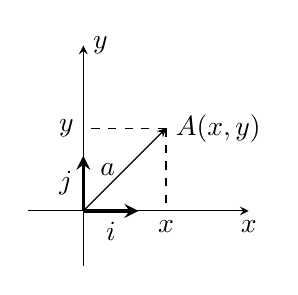
\begin{tikzpicture}[scale=0.7]
      \draw[->,>=stealth] (-1,0)--(3,0) node[below](x){$x$};
      \draw[->,>=stealth] (0,-1)--(0,3) node[right](y){$y$};
      \draw[very thick,->,>=stealth](0,0)--(1,0)node[midway,below](i) {$\bm{i}$};
      \draw[very thick,->,>=stealth](0,0)--(0,1)node[midway,left](j) {$\bm{j}$};
      \coordinate(A) at (1.5,1.5);
      \node[right](a1)at(1.5,1.5){$A(x,y)$};
      \draw[dashed](A)--++(-1.5,0)node[left](y){$y$};
      \draw[dashed](A)--++(0,-1.5)node[below](x){$x$};
      \draw[->,>=stealth](0,0)--(A) node[midway,left] (a) {$\bm{a}$};
    \end{tikzpicture}
    \end{center}
    \begin{description}
      \item[三点共线的判定] 若$ A,~B,~C $三点共线,有$ \vv{OA}=\lambda \vv{OB}+\mu\vv{OC}~(\lambda+\mu=1) $.或$\vv{AB}=\lambda \vv{AC}$.
      %\begin{enumerate}[1)]
      %
      %\end{enumerate}
    \end{description}
  \subsection{平面向量的坐标计算}
    \begin{enumerate}
      \item
        设点$ A(x_1,y_1),~B(x_2,y_2) $,则$ \vv{AB}=(x_2-x_1,y_2-y_1) $.\par
        一个向量的坐标等于表示此向量的有向线段的终点的坐标减去起始点的坐标.
      \item
        若$\bm{a}=\left(x_1,y_1\right),\bm{b}=\left(x_2,y_2\right)$.
        \begin{description}
          \item[加法:]
            $\bm{a}+\bm{b}=(x_1+x_2,y_1+y_2)$
            \begin{equation*}
            \begin{aligned}
            \bm{a}+\bm{b}=&\left(x_1\bm{i}+y_1\bm{j}\right)+\left(x_2\bm{i}+y_2\bm{j}\right)\\
            =&\left(x_1+x_2\right)\bm{i}+\left(y_1+y_2\right)\bm{j}\\
            \text{即:}\bm{a}+\bm{b}=&(x_1+x_2,y_1+y_2)
            \end{aligned}
            \end{equation*}
          \item[减法:] $\bm{a}-\bm{b}=\left(x_1-x_2,y_1-y_2\right)$.同加法可得
          \item[数乘:]
            $ \lambda \bm{a}=\left(\lambda x_1,\lambda y_1\right) $\begin{equation*}
            \begin{aligned}
             \lambda \bm{a} =&\lambda\left(x_1\bm{i}+y_1\bm{j}\right)=\lambda x_1\bm{i}+\lambda y_1\bm{j}\\
            =&\left(\lambda x_1,\lambda y_1\right)
            \end{aligned}
            \end{equation*}
          \item[模长]
           $\abs{\bm{a}}=\sqrt{x_1^2+y_1^2}$\qquad
           $\abs{\vv{AB}}=\sqrt{(x_2-x_1)^2+(y_2-y_1)^2}$\\
           \qquad $\abs{\bm{a}+\bm{b}}=\sqrt{(\bm{a}+\bm{b})^2}=\sqrt{\bm{a}^2+2\bm{a}\bm{\cdot}\bm{b}+\bm{b}^2}$\\
          \item[共线]$\bm{a} \varparallel \bm{b}\Leftrightarrow x_1y_2=y_2x_1 $\\
            由向量共线的性质知$ \bm{a} $与$ \bm{b}(\bm{b}\ne\bm{0}) $共线,当且仅当存在实数$ \lambda $使得$ \bm{a}=\lambda \bm{b} .$\\用坐标表示为:
            $$(x_1,y_1)=\lambda(x_2,y_2)$$
            即$$\Bigg\{\begin{aligned}
            x_1=&\lambda x_2\\
            y_1=&\lambda y_2
            \end{aligned}$$
            消去$ \lambda $得到\[x_1y_2-x_2y_1=0\]
          \item[垂直]
            $\bm{a}\perp\bm{b}\Leftrightarrow\bm{a}\bm{\cdot}\bm{b}=0\Leftrightarrow x_1x_2+y_1y_2=0 $
            \begin{proof}
              \begin{description}
                % \item[方法一]
                %   设$ \bm{a},~\bm{b} $所在直线分别为$ l_1,l_2 $,当$ \bm{a},~\bm{b} $所在直线的斜率都存在时,由直线垂直的性质,有$$ k_{l_1}\bm{\cdot}k_{l_2}=-1 $$
                %   其中$$ k_{l_1} =\dfrac{y_1-0}{x_1-0}=\dfrac{y_1}{x_1},\quad k_{l_2} =\dfrac{y_2-0}{x_2-0}=\dfrac{y_2}{x_2}$$
                %   即$$\dfrac{y_1}{x_1}\bm{\cdot}\dfrac{y_2}{x_2}=-1$$
                %   $$x_1x_2+y_1y_2=0$$
                % \item[方法二]
                  由向量的数量积性质,当$ \bm{a}\perp\bm{b} $时,
                  $\text{由}\cos\theta=\dfrac{\bm{a\cdot b}}{\abs{\bm{a}}\abs{\bm{b}}}\text{得到}$\\
                  \centering $\bm{a\cdot b}=0$
              \end{description}
            \end{proof}
        \end{description}
    \end{enumerate}
  \begin{exercise}{{\textbf{基础练习}}}
    \item%《习题化知识清单》P82知识1-3【平面向量基本定理】
      已知向量$\bm a=(1,2)$,$\bm b=(-2,3)$,$\bm c=(4,1)$,若用$\bm a$和$\bm b$表示$\bm c$,则$\bm c=$\tk.
      \begin{answer}
        $2\bm a-\bm b$
      \end{answer}
    \item%《习题化知识清单》P82知识2-1【向量坐标运算】
      设平面向量$\bm a=(3,5)$,$\bm b=(-2,1)$,则$\bm a-2\bm b=$\xz
      \xx{(7,3)}{(7,7)}{(1,7)}{(1,3)}
      \begin{answer}
        A
      \end{answer}
    \item%《习题化知识清单》P82知识2-2【向量坐标运算,单位向量】
      已知$\bm a=(3,4)$,则与$\bm a$同向的单位向量的坐标是\xz
      \xx{$(3,4)$}
       {$(-\dfrac{3}5,\dfrac{4}5)$}
       {$(-\dfrac{3}5,-\dfrac{4}5)$}
       {$(\dfrac{3}5,\dfrac{4}5)$}
      \begin{answer}
        D
      \end{answer}
    \item%《习题化知识清单》P82知识2-3【向量坐标运算,中点坐标公式】
      已知平面直角坐标系$xOy$内的三点分别是$A(2,-5)$,$B(3,4)$,$C(-1,-3)$,$D$为线段$BC$的中点,则向量$\vv{DA}$的坐标为\tk.
    \item%《习题化知识清单》P82知识3-1【向量共线】
      设向量$\bm a=(m,1)$,$\bm b=(1,m)$,如果$\bm a$与$\bm b$共线且方向相反,那么$m$的值为\xz
      \xx{$1$}{$-1$}{$\pm 1$}{$0$}
      \begin{answer}
        B
      \end{answer}
    \item%《习题化知识清单》P82知识3-3【向量共线,三角函数的定义】
      若$\bm a=\Bigl(\dfrac{3}2,\sin\alpha\Bigr)$,$\bm b=\Bigl(\sin\alpha,\dfrac{1}3\Bigr)$,且$\bm a\varparallel \bm b$,则锐角$\alpha$为\xz
      \xx{30\degree}{45\degree}{60\degree}{75\degree}
      \begin{answer}
        B
      \end{answer}
    \item%《习题化知识清单》P82知识3-4【向量共线坐标表示】
      若向量$\vv{OA}=(k,6)$,$\vv{OB}=(4,5)$,$\vv{OC}=(1-k,10)$,且$A$,$B$,$C$三点共线,则$k=$\tk.
      \begin{answer}
        $\dfrac{17}6$
      \end{answer}
  \end{exercise}
\section{平面向量的数量积}
  \subsection{定义}
    \begin{description}
      \item[定义] 已知两个非零向量$ \bm{a} $与$\bm{b}$,我们把数量$ \abs{\bm{a}}\abs{\bm{b}}\cos\theta $叫做$ \bm{a} $与$ \bm{b} $的\textbf{数量积}(又称点积、内积),记作$ \bm{a}\bm{\cdot}\bm{b} $,即\[\bm{a}\bm{\cdot}\bm{b}=\abs{\bm{a}}\abs{\bm{b}}\cos\theta\]
      其中$ \theta $为$ \bm{a} $与$ \bm{b} $的夹角.\\
      $\abs{\bm{a}}\cos\theta$($\abs{\bm{b}}\cos\theta$)叫做向量$\bm a$在$\bm b$方向上($\bm b$在$\bm a$方向上)的\textbf{投影},记作$\mathrm{Prj}_{\bm b}{\bm a}$(或$\mathrm{Prj}_{\bm b}{\bm a}$)
      \item[几何意义] 两个向量的数量积等于其中一个向量的模长与另一个向量在此向量方向上的投影的乘积\\%$ \bm{a}\bm{\cdot}\bm{b} $等于$\bm{a} $的模长$ \abs{\bm{a}} $与$ \bm{b} $在$ \bm{a} $的方向上的\textbf{投影}$ \abs{\bm{b}}\cos \theta $的乘积.\par
      {\kaishu \textbf{注:}当$ \theta=0 $时,$ \cos\theta=1 $,所以有$ \bm{a\cdot b}=\bm{\abs{a}\abs{b}} $;\\\phantom{注:\ }当$ \theta=90^{\circ} $时,有$ \cos\theta =0$,所以有$ \bm{a\cdot b}=0 $ \\\phantom{注:\ }当$ \theta=180^{\circ} $时,有$ \cos\theta =-1$,所以有$ \bm{a\cdot b}=\abs{\bm{a}}\abs{\bm{b}} $   }
      \item[数量积计算]
      \begin{equation*}+
      \begin{aligned}
      &\because \bm{a}=x_1\bm{i}+y_1\bm{j},~\bm{b}=x_2\bm{i}+y_2\bm{j},\\
      &\therefore \bm{a}\bm{\cdot}\bm{b}=(x_1\bm{i}+y_1\bm{j})\bm{\cdot}(x_2\bm{i}+y_2\bm{j})\\
      &\phantom{\therefore\bm{a}\bm{\cdot}\bm{b}~}=x_1x_2\bm{i}^2+x_1y_2\bm{i}\bm{\cdot}\bm{j}+x_2y_1\bm{i}\bm{\cdot}\bm{j}+y_1y_2\bm{j}^2.\\
      & \bm{i}^2=\bm{j}^2=1,\bm{i}\bm{\cdot}\bm{j}=\bm{j}\bm{\cdot}\bm{i}=0\\
      &\therefore \bm{a}\bm{\cdot}\bm{b}=x_1x_2+y_1y_2.
      \end{aligned}
      \end{equation*}
      \item[运算律]已知向量$\bm a$,$\bm b$,$\bm c$和实数$\lambda$,则:
        \begin{itemize}%[leftmargin=*]
          \item 交换律:$\bm{a}\cdot\bm{b}=\bm{b}\cdot\bm{a}$;
          \item 分配律:$(\bm a+\bm b)\cdot \bm c=\bm a\cdot\bm c+\bm b\cdot \bm c$;
          \item $(\lambda \bm a)\cdot\bm{b}=\lambda(\bm a\cdot\bm b)=\bm{a}\cdot(\lambda\bm{b})$.
        \end{itemize}
      \item[夹角公式] \[ \cos\theta=\dfrac{\bm{a}\bm{\cdot}\bm{b}}{\abs{\bm{a}}\abs{\bm{b}}}=\dfrac{x_1x_2+y_1y_2}{\sqrt{x_1^2+y_1^2}\sqrt{x_2^2+y_2^2}} \quad \left(\theta\in\left[0,\pi\right],~\theta\text{也写作}\left<\bm{a},\bm{b}\right>\right).\]
    \end{description}\par
    {\kaishu 直接求向量的数量积的方是近年高考的重点,其关键是根据向量的加减法则对向量进行基底分解.分解以后可以直接使用题目的已知条件,要么出现所要求的表达式(此时通过解一元一次方程).分解过程中,往往利用\CJKunderdot{垂直}将数量积消掉.\CJKunderdot{整体}的思想在数学中占据着极其重要的位置,求解整体的值时,往往不需要分别求出各个元素的值,而是将元素进行有效的分解、整合,提取有效的信息,从而求出整体的值.}
    %\subsection{求向量夹角的方法}
    %\begin{description}
    %\item[坐标法] $\cos\theta=\dfrac{x_1x_2+y_1y_2}{\sqrt{x_1^2+y_1^2}\sqrt{x_2^2+y_2^2}}$
    %\item[向量法] $\cos\theta=\dfrac{\bm{a}\bm{\cdot}\bm{b}}{\abs{\bm{a}}\abs{\bm{b}}}$
    %\end{description}
  \subsection{数量积相关补充}
    \begin{enumerate}[label=\circled{\arabic*}]
      \item 若$\bm{a}=\left(x,y\right)$,则$ \bm{a}\bm{\cdot}\bm{a}=\bm{a}^2=\abs{\bm{a}}^2=x^2+y^2 $;
      \item $ \left(\bm{a}\pm \bm{b}\right)^2=\abs{\bm{a}\pm \bm{b}}^2=\abs{\bm a}^2\pm2\bm{a}\bm{\cdot}\bm{b}+\abs{\bm b}^2=\bm{a}^2\pm2\bm{a}\bm{\cdot}\bm{b}+\bm{b}^2$;
      \item $\bm a^2-\bm b^2=(\bm a+\bm b)\cdot(\bm a-\bm b)=\abs{\bm a}^2-\abs{\bm b}^2$;
      \item $\bm a^2+\bm b^2=0\Leftrightarrow \bm a=\bm b=0$
      \item $\bigm|\abs{\bm{a}}-\abs{\bm{b}}\bigm|\le\abs{\bm{a\pm b}}\le\abs{\bm{a}}+\abs{\bm{b}}$;
      \item 若点$ A(x_1,y_1),~B(x_2,y_2) $,则$ \abs{\vv{AB}}=\sqrt{(x_2-x_1)^2+(y_2-y_1)^2} $;
      \item \textbf{柯西-施瓦兹不等式:}若$\bm{a}=\left(x_1,y_1\right),\bm{b}=\left(x_2,y_2\right)$,则:$$ -\abs{\bm{a}}\abs{\bm{b}}\le\bm{a}\bm{\cdot}\bm{b}\le\abs{\bm{a}}\abs{\bm{b}}\Leftrightarrow -\sqrt{x_1^2+y_1^2}\sqrt{x_2^2+y_2^2}\le x_1x_2+y_1y_2\le \sqrt{x_1^2+y_1^2}\sqrt{x_2^2+y_2^2}$$
      \item 若$ \abs{\bm{a}+\bm{b}}=\abs{\bm{a}-\bm{b}} $,则$ \bm{a}\perp\bm{b} $.对角线相等的平行四边形必然是矩形.
      \item 若$ \left(\bm{a}+\bm{b}\right)\perp\left(\bm{a}-\bm{b}\right) $,则$\abs{\bm{a}}=\abs{\bm{b}} $.对角线垂直的平行四边形必然是菱形.
      \item 平面上$ O,~A,~B $三点不共线,设$\vv{OA}=\bm{a}=(x_1,y_1) ,~\vv{OB}=\bm{b}=(x_2,y_2)$,则$$ S_{\triangle OAB}=\dfrac{1}{2}\sqrt{\abs{\bm{a}}^2\abs{\bm{b}}^2-\left(\bm{a}\bm{\cdot}\bm{b}\right)^2}=\dfrac{1}{2}\abs{x_1y_2-x_2y_1} .$$
      \item 给定两个长度为$ a $的平面向量$ \vv{OA},~\vv{OB} $,其夹角为$ \theta\in\left[0,\pi \right), ~$点$ C $在以$ O $为圆心的圆弧$ AB $上变动,若$ \vv{OC}=x\vv{OA}+y\vv{OB},~x,y\inR $,则$ x+y $的最大值为$ \sqrt{\dfrac{2}{\cos\theta+1}}. $
    \end{enumerate}
  \begin{exercise}{{\textbf{基础练习}}}
    \item%《习题化知识清单》P83知识1-1【数量积的定义、性质】
      在$\triangle{ABC}$中,$AB=BC=2$,$\angle{B}=\dfrac{\piup}4$,$AD$是边$BC$上的高,则$\vv{AD}\cdot\vv{AC}$的值为\xz
      \xx{0}{2}{4}{8}
      \begin{answer}
        B
      \end{answer}
    \item%《习题化知识清单》P83知识1-2【数量积的定义、性质】
      已知$\triangle{ABC}$中,$AB=AC=BC=6$,平面内一点$M$满足$\vv{BM}=\dfrac{2}3\vv{BC}-\dfrac{1}3\vv{BA}$,则$\vv{AC}\cdot\vv{MB}$等于\xz
      \xx{$-9$}{$-18$}{$12$}{$18$}
      \begin{answer}
        B
      \end{answer}
    \item%《习题化知识清单》P83知识2-2【向量的夹角】
      已知$\abs{\bm a}=2$,$\abs{\bm b}=4$,且$(\bm a+\bm b)\perp \bm a$,则$\bm a$与$\bm b$的夹角为\xz
      \xx{$\dfrac{2\piup}3$}
       {$\dfrac{\piup}3$}
       {$\dfrac{4\piup}3$}
       {$-\dfrac{2\piup}3$}
      \begin{answer}
        A
      \end{answer}
    \item%《习题化知识清单》P84知识4-2【数量积的坐标表示】
      已知$\bm a=(2,-3)$,$\bm b=(1,-2)$,且$\bm c\perp \bm a$,$\bm b\cdot\bm c=1$,则$\bm c$的坐标为\xz
      \xx{$(3,-2)$}{$(3,2)$}{$(-3,-2)$}{$(-3,2)$}
      \begin{answer}
        C
      \end{answer}
    \item%《习题化知识清单》P84知识4-3【数量积的坐标表示】
      在以$OA$为一边,$OB$为一条对角线的矩形中,$\vv{OA}=(-3,1)$,$\vv{OB}=(-2,k)$,则实数$k=$\xz
      \xx{$4\sqrt{3}$}{$3\sqrt{3}$}{$\dfrac{\sqrt{3}}2$}{$4$}
      \begin{answer}
        D
      \end{answer}
    \item%《习题化知识清单》P82知识2-4【向量的投影】
      已知点$A(-1,1)$,$B(1,2)$,$C(-2,-1)$,$D(3,4)$,则向量$\vv{CD}$在$\vv{AB}$方向上的投影为\tk.
      \begin{answer}
        $3\sqrt{5}$
      \end{answer}
    \item%《习题化知识清单》P84知识3-3【数量积的运算律】
      已知不共线向量$\bm a$,$\bm b$,$\abs{\bm a}=2$,$\abs{\bm b}=3$,$\bm a\cdot(\bm b-\bm a)=1$,则$\abs{\bm b-\bm a}=$\tk.
      \begin{answer}
        $\sqrt{3}$
      \end{answer}
    \item%《习题化知识清单》P84知识5-3【数量积的应用,运算律】
      已知$\abs{\bm a}=\abs{\bm b}=1$,$\bm a$,$\bm b$的夹角是直角,
      $\bm c=2\bm a+3\bm b$,$\bm d=k\bm a-4\bm b$,$\bm c\perp\bm d$,则$k=$\tk.
      \begin{answer}
        6
      \end{answer}
  \end{exercise}
\newpage
% \section{习题}
%   \begin{exercise}
%     \item%1平面向量的基本概念.pdf P3训练3
%       一辆汽车从$A $点出发向西行驶了100 km 到达$B $点,然后又改变方向向西偏北$50\degree$走了200 km到达$C$ 点,最后又改变方向,向东行驶了100 km 到达$D$ 点.\\
%       (1)作出向量$\vv{AB}$,$\vv{BC}$,$\vv{CD}$;\\
%       (2)求$\abs{\vv{AD}}$.\\
%     \vspace{4cm}\\
%     \begin{minipage}[b]{0.65\linewidth}
%     \item%LaTeX-master/xiangliang/xiangliangsorting.tex P10-p48
%       在$\triangle ABC$中,点$ M$,$N $满足$ \vv{AM}=2\vv{MC}$,$\vv{BN}=\vv{NC}$.若$\vv{MN}=x\vv{AB}+y\vv{AC}$,则$ x= $\tk;$ y= ~$ \tk.
%       \begin{answer}
%         $x=\dfrac12$;$y=-\dfrac16$
%       \end{answer}
%     \end{minipage}
%     \begin{minipage}[htbp!]{0.3\linewidth}
%       \begin{center}
%       \begin{tikzpicture}
%         \draw(0,0)node[below](B){\small$B$}--(1,0)node[below](N){\small$N$}--(2,0)node[below](C){\small$C$};
%         \draw (0,0)--(1.1,2.1)node[above](A){\small$A$}--(2,0);
%         \draw (1,0)--(1.1,2.1);
%         \draw(1,0)--($(1.1,2.1)!0.7!(2,0)$)node[right](M){\small$M$};
%       \end{tikzpicture}
%       \end{center}
%     \end{minipage}
%     \item
%       (2018届贵州遵义航天高级中学一模)如图所示,向量$\vv{OA}=\bm{a}$,$\vv{OB}=\bm{b}$,$\vv{OC}=\bm{c}$,$A$,$B$,$C$在一条直线上,且$\vv{AC}=3\vv{BC}$,则\xz
%       \begin{minipage}[b]{0.7\linewidth}
%         \xx{$\bm{c}=\dfrac32\bm{b}-\dfrac12\bm{a}$}
%           {$\bm{c}=\dfrac32\bm{a}-\dfrac12\bm{b}$}
%           {$\bm{c}=-\bm{a}+2\bm{b}$}
%           {$\bm{c}=\bm{a}+2\bm{b}$}
%       \end{minipage}\hfill
%       \begin{minipage}[htbp!]{0.3\linewidth}
%         \begin{center}
%         \begin{tikzpicture}
%           \coordinate[label=left:$O$](O)at(0,0);
%           \coordinate[label=right:$C$](C)at(3,0);
%           \coordinate[label=left:$A$](A)at(-1,2.5);
%           \coordinate[label=right:$B$](B)at($(A)!0.66!(C)$);
%           \draw (A)--(B)--(C)--cycle;
%           \draw[->,>=latex] (O)--(C);
%           \draw[->,>=latex] (O)--(A);
%           \draw[->,>=latex] (O)--(B);
%         \end{tikzpicture}
%         \end{center}
%       \end{minipage}
%       \begin{answer}
%         A
%       \end{answer}
%     \item
%       设向量$\bm a$,$\bm b$不共线,向量$\lambda\bm a+\bm b$与$\bm a+2\bm b$共线,则实数$\lambda=$\tk.
%       \begin{answer}
%         $\dfrac12$
%       \end{answer}
%     \vspace{2em}
%     \item
%       如图,在$\triangle ABC$中,$D$,$E$为边$AB$的两个三等分点,$\vv{CA}=3\bm a$,$\vv{CB}=2\bm b$,求$\vv{CD}$,$\vv{CE}$(用$\bm a$,$\bm b$表示).
%       \begin{flushright}
%         \begin{tikzpicture}
%           \coordinate[label=left:$B$](B)at(0,0);
%           \coordinate[label=right:$C$](C)at(2.5,0);
%           \coordinate[label=above:$A$](A)at(3,3);
%           \coordinate[label=above:$E$](E)at($(B)!0.33!(A)$);
%           \coordinate[label=above:$D$](D)at($(B)!0.66!(A)$);
%           \draw (A)--(B)--(C) --cycle;
%           \draw (C)--(D) (C)--(E);
%           \draw[->,>=latex] (C)--(A);
%           \draw[->,>=latex] (C)--(B);
%         \end{tikzpicture}
%       \end{flushright}
%       \begin{answer}
%         $\vv{CD}=2\bm a+\dfrac23\bm b$;$\vv{CE}=\bm a+\dfrac43\bm b$
%       \end{answer}
%     \item%1平面向量的基本概念.pdf P10例2
%       设$\bm a$,$\bm b$是不共线的两个非零向量.\\
%       (1)若$\vv{OA}=2\bm a-\bm b$,$\vv{OB}=3\bm a+\bm b$,$\vv{OC}=\bm a-3\bm b$,求证:$A$,$B$,$C$三点共线;\\
%       (2)若$8\bm a+k\bm b$与$k\bm a+\2\bm b$共线,求实数$k$的值;\\
%       (3)若$\vv{OM}=m\bm a$,$\vv{ON}=n\bm b$,$\vv{OP}=\alpha\bm a+\beta\bm b$,其中$m$,$n$,$\alpha$,$\beta$均为实数,且$m,n\neq 0$,若$M$,$P$,$N$三点共线,求证:$\dfrac{\alpha}m+\dfrac{\beta}n=1$
%       \begin{answer}
%         (1)$\because \vv{AB}=\bm a+2\bm b$,$\vv{CB}=2\bm a+4\bm b$;$\therefore \vv{CB}=2\vv{AB}$;
%         (2)$k=2\sqrt2$;
%       \end{answer}
%       \vspace{5cm}
%     \item
%       设点$G$为$\triangle ABC$重心,$D$,$E$,$F$分别为各边中点.试用向量证明:$AG=\dfrac23 AD$.
%       \begin{flushright}
%         \begin{tikzpicture}
%           \coordinate[label=left:$B$](B)at(0,0);
%           \coordinate[label=right:$C$](C)at(3,0);
%           \coordinate[label=above:$A$](A)at(2,2);
%           \coordinate[label=below:$D$](D)at($(B)!0.5!(C)$);
%           \coordinate[label=right:$E$](E)at($(A)!0.5!(C)$);
%           \coordinate[label=above:$F$](F)at($(B)!0.5!(A)$);
%           \coordinate[label=above:$G$](G)at($(D)!0.33!(A)$);
%           \draw (A)--(B)--(C) --cycle;
%           \draw (A)--(D) (B)--(E) (C)--(F);
%         \end{tikzpicture}
%       \end{flushright}
%     \vspace{2cm}
%   \end{exercise}
\clearpage
\section{课后作业}
  \begin{exercise}
    \item%1平面向量的基本概念.pdf P2-训练1
      判断下列结论是否正确(请在括号中打“\checkmark”或“\XSolidBrush”)\\
      (1)向量就是有向线段.(  )\\
      (2)如果$\abs{\vv{AB}}>\abs{\vv{CD}}$,那么$\vv{AB}>\vv{CD}$.(  )\\
      (3)力、速度和质量都是向量.(  )\\
      (4)若$\bm a$,$\bm b$都是单位向量,则$\bm a=\bm b$.(  )\\
      (5)若$\bm a=\bm b$,且$\bm a$与$\bm b$的起点相同,则终点也相同.(  )\\
      (6)零向量的大小为0,没有方向.(  )\\
      (7)两个具有公共终点的向量,一定是共线向量;\\
      (8)两个向量不能比较大小,但它们的模能比较大小;\\
      (9)$\lambda$,$\mu$为实数,若$\lambda\bm{a}=\mu\bm{b}$,则$\bm{a}$与$\bm{b}$共线.
      \begin{answer}
        (5)(8)正确,其余皆误.
      \end{answer}
    \item
      (2018·安徽淮北第一中学最后一卷)设$\bm{a}$,$\bm{b}$都是非零向量,下列四个条件,使$\dfrac{\bm{a}}{\abs{\bm{a}}}=\dfrac{\bm{b}}{\abs{\bm{b}}}$成立当且仅当\xz
      \xx{$\bm a=\bm b$}
      {$\bm a=2\bm b$}
      {$\bm a\varparallel\bm b$且$\abs{\bm a}=\abs{\bm b}$}
      {$\bm a\varparallel\bm b$且方向相同}
      \begin{answer}
        D
      \end{answer}
    \item
      已知四边形$ABCD$ 是菱形,则下列等式中成立的是\xz
      \xx{$\vv{AB}+\vv{BC}=\vv{CA}$}
        {$\vv{AB}+\vv{AC}=\vv{BC}$}
        {$\vv{AC}+\vv{BA}=\vv{AD}$}
        {$\vv{AC}+\vv{AD}=\vv{DC}$}
      \begin{answer}
        C
      \end{answer}
    % \item%1平面向量的基本概念.pdf P13-4
    %   已知$AM$ 是$\triangle ABC$ 的边$BC$ 上的中线,若$\vv{AB}=\bm a$,$\vv{AC}=\bm b$,则$\vv{AM}$等于\xz
    %   \xx{$\dfrac12(\bm a-\bm b)$}
    %     {$-\dfrac12(\bm a-\bm b)$}
    %     {$\dfrac12(\bm a+\bm b)$}
    %     {$-\dfrac12(\bm a+\bm b)$}
    %   \begin{answer}
    %     C
    %   \end{answer}
    \item%《习题化知识清单》P81知识4-1【向量共线】
      已知向量$\bm a$、$\bm b$不共线,$\bm c=k\bm a+\bm b({k\in\mathbb{R}})$,$\bm d=\bm a-\bm b$。如果$\bm c\varparallel \bm d$,那么\xz
      \xx{$k=1$且$\bm c$与$\bm d$同向}
        {$k=1$且$\bm c$与$\bm d$反向}
        {$k=-1$且$\bm c$与$\bm d$同向}
        {$k=-1$且$\bm c$与$\bm d$反向}
      \begin{answer}
        D
      \end{answer}
    \item%《习题化知识清单》P82方法1【平面向量基本定理应用】
      在平行四边形$ABCD$中,$M$,$N$分别为$DC$,$BC$的中点,已知$\vv{AM}=\bm c$,$\vv{AN}=\bm d$,试用$\bm c$,$\bm d$表示$\vv{AB}=$\tk,$\vv{AD}=$\tk.
      \begin{answer}
        $\vv{AB}=\dfrac{2}3(2\bm d-\bm c)$,$\vv{AD}=\dfrac{2}3(2\bm c-\bm d)$
      \end{answer}
    \item%《习题化知识清单》P83方法2【向量共线条件应用】
      平面内给定三个向量$\bm a=(3,2)$,$\bm b=(-1,2)$,$\bm c=(4,1)$,则\\
      (1)若$(\bm a+k\bm c)\varparallel(2\bm b-\bm a)$,则实数$k=$\tk;\\
      (2)设$\bm d=(x,y)$满足$(\bm d-\bm c) \varparallel (\bm a+\bm b)$且$\abs{\bm d-\bm c}=1$,则$\bm d=$\tk.
      \begin{answer}
        (1)$k=-\dfrac{16}{13}$;(2)$\bm d=\Bigl(\dfrac{20+\sqrt{5}}5,\dfrac{5+2\sqrt{5}}5\Bigr)$或$\Bigl(\dfrac{20-\sqrt{5}}5,\dfrac{5-2\sqrt{5}}5\Bigr)$
  \end{answer}
    \item%《习题化知识清单》P84方法1【求向量夹角基本方法】
      已知$\abs{\bm a}=1$,$\abs{\bm b}=2$,$\bm a$与$\bm b$的夹角为120\degree,则使$\bm a+k\bm b$与$k\bm a+\bm b$的夹角为锐角的实数$k$的取值范围是\tk.
      \begin{answer}
        $\Bigl(\dfrac{5-\sqrt{21}}2,1\Bigr) \bigcup \Bigl(1,\dfrac{5-\sqrt{21}}2 \Bigr)$
      \end{answer}
    \item%《习题化知识清单》P84方法2【求向量模的基本方法】
      已知向量$\bm a$,$\bm b$夹角为45\degree,且$\abs{\bm a}=1$,$\abs{2\bm a-\bm b}=\sqrt{10}$,则$\abs{\bm b}=$\tk.
      \begin{answer}
        $3\sqrt{2}$
      \end{answer}
    \item%《习题化知识清单》P85方法4
      在矩形$ABCD$中,$AB=\sqrt{2}$,$BC=2$,点$E$为$BC$的中点,点$F$在边$CD$上,若$\vv{AB}\cdot\vv{AF}=\sqrt{2}$,则$\vv{AE}\cdot\vv{BF}$的值是\tk.
      \begin{answer}
        $\sqrt{2}$
      \end{answer}
    \item%《习题化知识清单》P85方法4-2
      已知正方形$ABCD$的边长为1,点$E$是$AB$边上的动点,则$\vv{DE}\cdot\vv{CB}$的值为\tk;$\vv{DE}\cdot\vv{DC}$的最大值为\tk.
      \begin{answer}
        1;1
      \end{answer}
    \item%1平面向量的基本概念.pdf P13-10
      化简:\\
      \circled{1} $\vv{BC}+\vv{AB}$; \hspace{2em} \circled{2} $\vv{DB}+\vv{CD}+\vv{BC}$;\\
      \circled{3} $\vv{AB}-\vv{FD}+\vv{CD}-\vv{CB}+\vv{FA}$;\hspace{2em} \circled{4} $(\vv{AC}+\vv{BO}+\vv{OA})-(\vv{DC}-\vv{DO}-\vv{OB})$;\\
      \begin{answer}
        \circled{1}$\vv{AC}$;\circled{2}$\bm 0$;\circled{3}$\bm 0$;\circled{4}$\bm 0$
      \end{answer}
    \vspace{1.5cm}
    % \item%1平面向量的基本概念.pdf P8训练5
    %   一架飞机从$A$ 地按北偏东$35\degree$的方向飞行800 km 到达$B$ 地接到受伤人员,然后又从$B$ 地按南偏东$55\degree$的方向飞行600 km 送往$C $地医院,求这架飞机飞行的路程及两次位移的和.
    %   \begin{answer}
    %     路程1400km,位移1000km.
    %   \end{answer}
    % \vspace{4cm}
    \item%《高中数学竞赛培优教程+一试(李名德 主编)》.pdf P115-例5.10
      已知向量$\bm a=(\cos\alpha,\sin\alpha)$,$\bm b=(\cos\beta,\sin\beta)$,且$\bm a$,$\bm b$满足关系$\abs{k\bm a+\bm b}=\sqrt{3}\abs{\bm a-k\bm b}$($k>0$).\\
      (1)求将$\bm a$与$\bm b$的数量积用$k$表示的解析式$f(k)$;\\
      (2)\hspace{5pt}$\bm a$能否和$\bm b$垂直?$\bm a$能否和$\bm b$平行?若不能,则说明理由;若能,则求出对应的$k$值;\\
      (3)求$\bm a$与$\bm b$夹角的最大值.
      \begin{answer}
        (1)$f(k)=\dfrac{k^2+1}{4k} (k>0)$;
        (2)$\bm a$与$\bm b$不可能垂直;当$k=2\pm\sqrt{3}$时,$\bm a\varparallel \bm b$;
        (3)60\degree
      \end{answer}
    \vspace{7cm}
    \item
      设点$G$为$\triangle ABC$重心,$D$,$E$,$F$分别为各边中点.\\
      (1)试用向量证明:三角形三条中线共点;
      (2)求$\vv{AD}+\vv{BE}+\vv{CF}$.
      \begin{flushright}
        \begin{tikzpicture}
          \coordinate[label=left:$B$](B)at(0,0);
          \coordinate[label=right:$C$](C)at(3,0);
          \coordinate[label=above:$A$](A)at(2,2);
          \coordinate[label=below:$D$](D)at($(B)!0.5!(C)$);
          \coordinate[label=right:$E$](E)at($(A)!0.5!(C)$);
          \coordinate[label=above:$F$](F)at($(B)!0.5!(A)$);
          \coordinate[label=above:$G$](G)at($(D)!0.33!(A)$);
          \draw (A)--(B)--(C) --cycle;
          \draw (A)--(D) (B)--(E) (C)--(F);
        \end{tikzpicture}
      \end{flushright}
    \vspace{5cm}
    \item%《习题化知识清单》P91单元检测16【三点共线,向量共线】
      设两个非零向量$\bm a$与$\bm b$不共线\\
      (1)若$\vv{AB}=\bm a+\bm b$,$\vv{BC}=2\bm a+8\bm b$,$\vv{CD}=3(\bm a-\bm b)$,求证:$A$,$B$,$D$三点共线;\\
      (2)试确定实数$k$,使$k\bm a+\bm b$与$\bm a+k\bm b$共线.
      \begin{answer}
        (1)略;(2)$k=\pm1$
      \end{answer}
    \vspace{5cm}
    \item
      已知$\vv{OA}=\lambda\vv{OB}+\mu\vv{OC}$($\lambda,\mu\in\mathbb{R}$),若$\lambda+\mu=1$,求证:点$A$,$B$,$C$三点共线.\\
    \vspace{4cm}
    \item
      【定比分点坐标公式】如图,设$P$为$\triangle ABO$边$AB$上一点.设$\vv{OA}=\bm a$,$\vv{OB}=\bm b$\vspace{8pt}\\
      (1)求证:$\vv{OP}=\dfrac{\abs{\vv{PB}}}{\abs{\bm b-\bm a}}\bm a+\dfrac{\abs{\vv{PA}}}{\abs{\bm b-\bm a}}\bm b$;\vspace{8pt}\\
      (2)设$\vv{AP}=\lambda\vv{PB}$,求证:$\vv{OP}=\dfrac{\bm a+\lambda\bm b}{1+\lambda}$
      \begin{flushright}
        \begin{tikzpicture}
          \coordinate[label=left:$O$](O)at(0,0);
          \coordinate[label=right:$A$](A)at(3,0);
          \coordinate[label=above:$B$](B)at(2,2);
          \coordinate[label=right:$P$](P)at($(B)!0.4!(A)$);
          \draw (A)--(B)--(O) --cycle;
          \draw[->,>=latex] (O)--(A);
          \draw[->,>=latex] (O)--(B);
          \draw[->,>=latex] (O)--(P);
        \end{tikzpicture}
      \end{flushright}
    \vspace{5cm}
    \item%《高中数学竞赛培优教程+一试(李名德 主编)》.pdf P118-例5.14【2004年湖北高考题】
      (2004年湖北高考题)在$\mathrm{Rt}\triangle{ABC}$中,已知$BC=a$,若长为$2a$的线段$PQ$以点$A$为中点,问$\vv{PQ}$与$\vv{BC}$的夹角$\theta$取何值时$\vv{BP}\cdot\vv{CQ}$的值最大?并求出这个最大值.\\
      \begin{answer}
        $\theta=0$时,$\vv{BP}\cdot\vv{CQ}$取最大值0.
      \end{answer}
  \end{exercise}
\stopexercise
\newpage
\section{部分参考答案}
\begin{multicols}{2}
  \printanswer
\end{multicols}

  % % 节录自b5-FinExRev.tex
\Topic{平面向量复习}
  \Teach{}
  \Grade{高一}
  % \Name{郑皓天}\FirstTime{20181207}\CurrentTime{20181207}
  % \Name{林叶}\FirstTime{20180908}\CurrentTime{20181125}
  %\Name{1v2}\FirstTime{20181028}\CurrentTime{20181117}
  % \Name{林叶}\FirstTime{20180908}\CurrentTime{20181125}
  % \Name{郭文镔}\FirstTime{20181111}\CurrentTime{20181117}
  % \Name{马灿威}\FirstTime{20181111}\CurrentTime{20181111}
  \Name{黄亭燏}\FirstTime{20181231}\CurrentTime{20190112}
  \newtheorem*{Theorem}{定理}
  \makefront
\vspace{-1.5em}
\startexercise
\section{要点归纳}
  \subsection{五种常见向量}
    \begin{enumerate}[label=\arabic*)]
      \item 单位向量:模为1的向量.
      \item 零向量:模为0的向量.
      \item 平行(共线向量):方向相同或相反或其一为零向量的两个向量.
      \item 相等向量:模相等,方向相同的向量.
      \item 相反向量:模相等,方向相反的向量.
    \end{enumerate}
  \subsection{平面向量运算律}
    \begin{enumerate}[label=\arabic*)]
      \item 交换律:
        $\bm a+\bm b=\bm b+\bm a$,\quad
        $\bm a\cdot\bm b=\bm b\cdot\bm a$
      \item 结合律:
        $(\bm{a}+\bm{b})+\bm{c}=\bm{a}+(\bm{b}+\bm{c})$,\quad
        $(\lambda \bm a)\cdot\bm{b}=\lambda(\bm a\cdot\bm b)=\bm{a}\cdot(\lambda\bm{b})$
      \item 分配律:
        $(\lambda+\mu)\bm{a}=\lambda\bm{a}+\mu\bm{a}$,\quad
        $\lambda(\bm{a}+\bm{b})=\lambda\bm{a}+\lambda\bm{b}$,\quad
        $(\bm a+\bm b)\cdot \bm c=\bm a\cdot\bm c+\bm b\cdot \bm c$
      \item 重要公式:(记号$\bm a^2=\bm a\cdot\bm a$)
        $(\bm a+\bm b)(\bm a-\bm b)=\bm a^2-\bm b^2$,\quad
        $(\bm a\pm\bm b)^2=\bm a^2\pm2\bm a\cdot\bm b+\bm b^2$.
    \end{enumerate}
  \subsection{两个重要定理}
    \begin{enumerate}[label=\arabic*)]
      \item 向量共线定理:
        向量$\bm{a}~(\bm{a}\ne\bm{0})$与向量$\bm{b}$共线,当且仅当存在唯一的实数$ \lambda $,使得$\bm{b}=\lambda\bm{a}$.\\
        {\kaishu
         证明三点共线的方法:\circled{1}$\vv{AB}=\lambda\vv{AC}$,则$A$,$B$,$C$三点共线;\circled{2}$\vv{OA}=\lambda\vv{OB}+\mu\vv{OC}$,若$\lambda+\mu=1$,则$A$,$B$,$C$三点共线.
        }
      \item 平面向量基本定理:
        如果$ \bm{e}_1,\bm{e}_2 $是同一平面内的两个\CJKunderdot{不共线}的向量,
        则那么对于这一平面内的任意向量$ \bm{a} $,有且只有一对实数$ \lambda_1,~\lambda_2 $,使$\bm{a}=\lambda_1\bm{e}_1+\lambda_2\bm{e}_2$.
        其中,不共线的向量$\bm{e}_1, \bm{e}_2$叫做表示这一平面内所有向量的一组\CJKunderdot{基底}.\\
        {\kaishu 平面向量基本定理应用技巧:
          \begin{enumerate}[label=\circled{\arabic*}]
            \item 构造某一向量在同一基底下的两种不同表达形式,
              根据向量分解的唯一性求解.即:\\
              {\kaishu 以$\bm e_1$,$\bm e_2$为基底,且$\bm a=x_1\bm e_1+y_1\bm e_2=x_2\bm e_1+y_2\bm e_2$,则$\begin{cases}x_1=x_2\\y_1=y_2\end{cases}$}
            \item 构造两个共线向量在同一基底下的表达形式,
              根据向量共线定理求解.即:\\
              {\kaishu 以$\bm e_1$,$\bm e_2$为基底,且$\bm a=x_1\bm e_1+y_1\bm e_2$,$\bm b=x_2\bm e_1+y_2\bm e_2$,且$\bm a\varparallel\bm b$,则$x_1y_2-x_2y_1=0$}
            \item 将题目中的已知条件转化成
              $\lambda_1\bm e_1+\lambda_2\bm e_2=\bm 0$的形式($\bm e_1$,$\bm e_2$不共线),根据$\lambda_1=\lambda_2=0$求解.
          \end{enumerate}}
    \end{enumerate}
  \subsection{平面向量平行、垂直的等价条件}
    设$\bm a=(x_1,y_1)$,$\bm b=(x_2,y_2)$,则:
    \begin{enumerate}[label=\arabic*)]
      \item $\bm a\varparallel\bm b$$\Leftrightarrow$$x_1y_2-x_2y_1=0$.
      \item $\bm a\perp\bm b$
            $\Leftrightarrow$$\bm a\cdot\bm b=0$
            $\Leftrightarrow$$x_1x_2+y_1y_2=0$.
    \end{enumerate}
  \subsection{平面向量数量积相关量求解}
    \begin{enumerate}[label=\arabic*)]
      \item 向量夹角:设$\bm a=(x_1,y_1)$,$\bm b=(x_2,y_2)$,则
        $\cos\vangle{\bm a}{\bm b}=\dfrac{\bm{a}\bm{\cdot}\bm{b}}{\abs{\bm{a}}\abs{\bm{b}}}=\dfrac{x_1x_2+y_1y_2}{\sqrt{x_1^2+y_1^2}\sqrt{x_2^2+y_2^2}} \quad \left(\vangle{\bm a}{\bm b}\in\left[0,\piup\right]$
      \item 向量模长:若$\bm a=(x,y)$,则$\abs{\bm a}=\sqrt{\bm a\cdot\bm a}=\sqrt{x^2+y^2}$
      \item 向量投影:向量$\bm a$在$\bm b$方向上的投影为  $\abs{\bm{a}}\cos\theta=\dfrac{\bm a\cdot\bm b}{\abs{\bm b}}$
    \end{enumerate}
\begin{exercise}{\textbf{习题}}
  \item%【向量的线性运算】
    (2017 \textbullet {\kaishu 广东深圳二模})如图所示,正方形$ABCD$中,$M$是$BC$的中点,若$\vv{AC}=\lambda\vv{AM}+\mu\vv{BD}$,则$\lambda+\mu$等于\xz
    \xx{$\dfrac{4}3$}
     {$\dfrac{5}3$}
     {$\dfrac{15}8$}
     {$2$}
    \begin{center}
      \begin{tikzpicture}
        \coordinate[label=left:$A$](A)at(0,0);
        \coordinate[label=right:$B$](B)at(3.5,0);
        \coordinate[label=left:$D$](D)at(0,3.5);
        \coordinate[label=right:$C$](C)at(3.5,3.5);
        \coordinate[label=right:$M$](M)at($(B)!0.5!(C)$);
        \draw (A)--(B)--(C)--(D)--cycle;
        \draw[->,>=latex] (A)--(C);
        \draw[->,>=latex] (A)--(M);
        \draw[->,>=latex] (B)--(D);
      \end{tikzpicture}
    \end{center}
    \begin{answer}
      B
    \end{answer}
  \item%福州一中学2016-2017学年高一下学期期末考试数学…….doc-3【向量共线】
    % (2017 \textbullet {\kaishu 福州一中} 3)
    已知向量$\bm a$,$\bm b$不共线,且$\bm c=\lambda\bm a+\bm b$,$\bm d=\bm a+(2\lambda-1)\bm b$,若$\bm c$与$\bm d$方向相反,则实数$\lambda$的值为\xz
    \xx{$1$}
     {$-\dfrac12$}
     {$1$或$-\dfrac12$}
     {$-1$或$-\dfrac12$}
    \begin{answer}
      B
    \end{answer}
  \item%福州三中2017高一下数学期末卷…….doc-5【向量投影,基底表示】
    % (2017 \textbullet {\kaishu 福州三中} 5)
    设$\bm e_1$,$\bm e_2$为单位向量,且$\bm e_1$,$\bm e_2$的夹角为$\dfrac{\piup}3$,若$\bm a=\bm e_1-3\bm e_2$,$\bm b=\bm e_1+\bm e_2$,则向量$\bm a$在$\bm b$方向上的射影为\xz
    \xx{$-\sqrt3$}
     {$\sqrt3$}
     {$-\dfrac{\sqrt{10}}5$}
     {$\dfrac{\sqrt{10}}5$}
    \begin{answer}
      A
    \end{answer}
  \item%【向量坐标法在平面几何的应用,三角函数定义】
    %如图,
    半径为$\sqrt{3}$的扇形$AOB$的圆心角为120\degree,点$C$在$\arc{AB}$上,且$\angle{COB}=30\degree$,若$\vv{OC}=\lambda\vv{OA}+\mu\vv{OB}$,则$\lambda+\mu$等于\xz
    \xx{$\sqrt{3}$}
     {$\dfrac{\sqrt{3}}3$}
     {$\dfrac{4\sqrt{3}}3$}
     {$2\sqrt{3}$}
    \begin{answer}
      A
    \end{answer}
  \item%【平面向量几何应用:垂直问题】
    直角坐标系$xOy$中,$\vv{AB}=(2,1)$,$\vv{AC}=(3,k)$,若$\triangle{ABC}$是直角三角形,则$k$的可能值个数是\xz
    \xx{1}{2}{3}{4}
    \begin{answer}
      B
    \end{answer}
  \item%福建师大附中2016-2017高一下期末考试数学试题…….doc-6【数量积,三角形形状】
    % (2017 \textbullet {\kaishu 师大附中} 6)
    若点$O$是$\triangle{ABC}$平面内一点,且满足$(\vv{OB}-\vv{OC})\cdot(\vv{OB}+\vv{OC}-2\vv{OA})=0$,则$\triangle{ABC}$形状为\xz
    \xx{钝角三角形}{等腰三角形}{直角三角形}{锐角三角形}
    \begin{answer}
      B
    \end{answer}
  \item%福州三中2017高一下数学期末卷…….doc-16【向量投影,基底表示】
    % (2017 \textbullet {\kaishu 福州三中} 16)
    已知$\bm a$,$\bm b$是平面内两个相互垂直的单位向量,若向量$\bm c$满足$(\bm a-\bm c)\cdot(\bm b-\bm c)=0$,则$|\bm c|$的最大值是\tk.
    \begin{answer}
      $\sqrt2$
    \end{answer}
  \item%%福建师大附中2016-2017高一下期末考试数学试题…….doc-15【向量夹角,线性运算模长】
    % (2017 \textbullet {\kaishu 师大附中} 15)
    已知单位向量$\bm a$,$\bm b$的夹角为$\dfracp{}3$,那么$|\bm a-2\bm b|=$\tk.
    \begin{answer}
      $\sqrt3$
    \end{answer}
  \item%【平面向量的模与夹角】
    已知$\triangle{ABC}$是正三角形,若$\vv{AC}-\lambda\vv{AB}$与向量$\vv{AC}$的夹角大于90\degree,则实数$\lambda$的取值范围是\tk.
    \begin{answer}
      $(2,+\infty)$
    \end{answer}
  \item%福建师大附中2016-2017高一下期末考试数学试题…….doc-17【数量积,几何】
    % (2017 \textbullet {\kaishu 师大附中} 17)
    在$\triangle{ABC}$中,$|\vv{AD}|=|\vv{BD}|=|\vv{CD}|$,$|\vv{AB}|=3$,则$\vv{AB}\cdot\vv{AD}=$\tk.
    \begin{answer}
      $\dfrac92$
    \end{answer}
  \item%【向量坐标法在平面几何的应用,直线方程】
    在$\mathrm{Rt}\triangle{ABC}$中,$CA=CB=2$,$M$,$N$是斜边$AB$上的两个动点,且$MN=\sqrt{2}$,则$\vv{CM}\cdot\vv{CN}$的取值范围是\tk.
    \begin{answer}
      $\Bigl[\dfrac{3}2,2\Bigr]$
    \end{answer}
  \item%福州一中学2016-2017学年高一下学期期末考试数学…….doc-14【数量积,外心】
    % (2017 \textbullet {\kaishu 福州一中} 14)
    $\triangle{ABC}$中,$CA=4$,$CB=6$,点$O$为$\triangle{ABC}$的外心,则$\vv{CO}\cdot\vv{AB}=$\tk.
    \begin{answer}
      5
    \end{answer}
  \item%福建师大附中2016-2017高一下期末考试数学试题…….doc-19【向量共线、夹角、模长】
    % (2017 \textbullet {\kaishu 师大附中} 19)
    已知$\bm a$,$\bm b$为两个不共线向量,$\abs{\bm a}=2$,$\abs{\bm b}=1$,$\bm c=2\bm a-\bm b$,$\bm d=\bm a+k\bm b$.\\
    (I)若$\bm c\varparallel\bm d$,求实数$k$;\\
    (II)若$k=-7$,且$\bm c\perp\bm d$,求$\bm a$与$\bm b$的夹角.
    \begin{answer}
      (I)$k=-\dfrac12$
      (II)$\vangle{\bm a}{\bm b}=\dfrac{\piup}3$
    \end{answer}
  \vspace{3cm}
  \item%福州一中学2016-2017学年高一下学期期末考试数学…….doc-15【数量积,垂直】
    % (2017 \textbullet {\kaishu 福州一中} 15)
    已知$\bm a=(\cos\alpha,k\sin\alpha)$,$\bm b=(\cos\beta,\sin\beta)$($k>0$,$0<\alpha<\beta<\dfrac{\piup}2$),且$\bm a+\bm b$与$\bm a-\bm b$相互垂直.\\
    (1)求$k$的值;\\
    (2)若$\bm a\cdot\bm b=\dfrac45$且$\cos\beta=\dfrac35$,求$\sin\alpha$的值.
    \begin{answer}
      (1)$k=1$;
      (2)$\sin\alpha=\dfrac7{25}$
    \end{answer}
    \vspace{4cm}
  \vspace{3.5cm}
  \item%【平面向量基本定理】
    在$\triangle{OAB}$的边$OA$,$OB$上分别取点$M$,$N$,使得$\vv{OA}=3\vv{OM}$,$\vv{OB}=4\vv{ON}$,设线段$AN$与$BM$交于点$P$,
    记$\vv{OA}=\bm a$,$\vv{OB}=\bm b$,用$\bm a$,$\bm b$表示向量$\vv{OP}$.
    \begin{answer}
      $\vv{OP}=\dfrac3{11}\bm a+\dfrac3{11}\bm b$
    \end{answer}
  \vspace{9cm}
  \item%【平面向量基本定理】
    在$\triangle{OAB}$中,$\vv{OA}=4\vv{OC}$,$\vv{OB}=2\vv{OD}$,设线段$AD$与$BC$交于点$M$,
    记$\vv{OA}=\bm a$,$\vv{OB}=\bm b$.\\
    (1)用$\bm a$,$\bm b$表示向量$\vv{OP}$.\\
    (2)已知在线段$AC$上取一点$E$,在线段$BD$上取一点$F$,使$EF$过点$M$,设$\vv{OE}=p\vv{OA}$,$\vv{OF}=q\vv{OA}$,求证$\dfrac1{7p}+\dfrac3{7q}=1$
    \begin{answer}
      (1)$\vv{OP}=\dfrac17\bm a+\dfrac37\bm b$
      (2)略
    \end{answer}
  \vspace{9cm}
\end{exercise}

\newpage
\section{课后作业}
\begin{exercise}
  \item%【向量的线性运算】
    若点$D$在$\triangle{ABC}$的边$BC$上,且$\vv{CD}=4\vv{DB}=r\vv{AB}+s\vv{AC}$,则$3r+s$的值为\xz
    \xx{$\dfrac{16}5$}
     {$\dfrac{12}5$}
     {$\dfrac{8}5$}
     {$\dfrac{4}5$}
    \begin{answer}
      C
    \end{answer}
  \item%福州屏东中学2016-2017学年高一下学期期末考试数学试题.doc-4【向量共线】
    % (2017 \textbullet {\kaishu 屏东中学} 4)
    若$A(-1,1)$,$B(1,3)$,$C(x,5)$,且$\vv{AB}=\lambda\vv{BC}$,则实数$\lambda$等于\xz
    \xx{1}{2}{3}{4}
    \begin{answer}
      1
    \end{answer}
  \item%福建师大附中2016-2017高一下期末考试数学试题…….doc-3【向量投影,坐标表示】
    % (2017 \textbullet {\kaishu 师大附中} 3)
    若$\bm a=(2,1)$,$\bm b=(3,4)$,则向量$\bm b$在向量$\bm a$方向上的投影为\xz
    \xx{$2\sqrt5$}
     {$2$}
     {$\sqrt5$}
     {$10$}
    \begin{answer}
      A
    \end{answer}
  \item%【向量表示】
    设$D$为$\triangle{ABC}$所在平面内一点,$\vv{BD}=3\vv{CD}$,则\xz
    \xx{$\vv{AD}=-\dfrac13\vv{AB}+\dfrac43\vv{AC}$}
     {$\vv{AD}=\dfrac43\vv{AB}-\dfrac13\vv{AC}$}
     {$\vv{AD}=\dfrac23\vv{AB}-\dfrac12\vv{AC}$}
     {$\vv{AD}=-\dfrac12\vv{AB}+\dfrac32\vv{AC}$}
    \begin{answer}
      D
    \end{answer}
  \item%【向量夹角、模长】
    已知$|\bm a|=1$,$\bm a\cdot\bm b=\dfrac12$,$|\bm a-\bm b|^2=1$,则$\bm a$与$\bm b$的夹角等于\xz
    \xx{30\degree}{45\degree}{60\degree}{120\degree}
    \begin{answer}
      C
    \end{answer}
  \item%【向量共线】
    已知向量$\bm a=(2,3)$,$\bm b=(-1,2)$,若$m\bm a+4\bm b$与$\bm a-2\bm b$共线,则$m$的值为\xz
    \xx{$\dfrac12$}{$2$}{$-\dfrac12$}{$-2$}
    \begin{answer}
      D
    \end{answer}
  \item%【向量几何应用】
    在平面四边形$ABCD$中,若$AC=3$,$BD=2$,则$(\vv{AB}+\vv{DC})\cdot(\vv{AC}+\vv{BD})=$\tk.
    \begin{answer}
      5
    \end{answer}
  \item%【向量垂直】
    平面向量$\bm a=(\sqrt{3},-1)$,$\bm=\Bp{\dfrac12,\dfrac{\sqrt3}2}$,若存在不同时为0的实数$k$和$t$,使$\bm x=\bm a+(t^2-3)\bm b$,$\bm y=-k\bm a+t\bm b$,且$\bm x\perp\bm y$,试求函数关系式$k=f(t)$.
    \begin{answer}
      $k=f(t)=\dfrac14(t^3-3t)$
    \end{answer}
  \vspace{2.5cm}
  \item%福州三中2017高一下数学期末卷…….doc-18【向量垂直,模长,共线】
    % (2017 \textbullet {\kaishu 福州三中} 18)
    平面内的向量$\bm a=(3,2)$,$\bm b=(-1,2)$,$\bm c=(4,1)$.\\
    (I)若$(\bm a+k\bm c)\perp(2\bm b-\bm a)$,求实数$k$的值;\\
    (II)若向量$\bm d$满足$\bm d\varparallel\bm c$,且$\abs{\bm d}=\sqrt{34}$,求向量$\bm d$的坐标.
    \begin{answer}
      (I)$k=-\dfrac{11}{18}$
      (II)$\bm d=(4\sqrt2,\sqrt2)$或$\bm d=(-4\sqrt2,-\sqrt2)$
    \end{answer}
  \vspace{5cm}
  \item
    已知点$P$是$\triangle{ABC}$内一点,且满足条件$\vv{AP}+\vv{AP}+\vv{AP}=\bm 0$,设点$Q$为$CP$的延长线与$AB$的交点,令$\vv{CP}=\bm p$,试用向量$\bm p$表示$\vv{CQ}$.
    \begin{answer}
      $\vv{CQ}=2\bm p$
    \end{answer}
  \vspace{6cm}
  \item%《2018天利38套:高考真题单元专题训练(文)》专题18平面向量的概念与运算 P63p31【2010•江苏】
    (2010 \textbullet {\kaishu 江苏})
    在平面直角坐标系$xOy$中,已知点$A(-1,-2)$,$B(2,3)$,$C(-2,-1)$.\\
    (I)求以线段$AB$,$AC$为邻边的平行四边形的两条对角线的长;\\
    (II)设实数$t$满足$(\vv{AB}-t\vv{OC})\cdot\vv{OC}=0$,求$t$的值.
    \begin{answer}
      (I)两条对角线长分别为$4\sqrt2$,$2\sqrt{10}$;
      (II)$t=-\dfrac{11}5$
    \end{answer}
  \item%《2018天利38套:高考真题单元专题训练(理)ISBN978-7-223-03438-8》专题18平面向量的应用 P72p17【2014•陕西】
    (2014 \textbullet {\kaishu 陕西})
    在直角坐标系$xOy$中,已知点$A(1,1)$,$B(2,3)$,$C(3,2)$,点$P(x,y)$在$\triangle{ABC}$三边围成的区域(含边界)上.\\
    (I)若$\vv{PA}+\vv{PB}+\vv{PC}=\bm 0$,求$\abs{\vv{OP}}$;\\
    (II)设$\vv{OP}=m\vv{AB}+n\vv{AC}$($m,n\inR$),用$x$,$y$表示$m-n$,并求$m-n$的最大值.
    \begin{answer}
      (I)$\abs{\vv{OP}}=2\sqrt2$;
      (II)$(x,y)=(m+2n,2m+n)$,$m-n$最大值为1.
    \end{answer}
\end{exercise}
\stopexercise

\newpage
\section{参考答案}
\begin{multicols}{2}
  \printanswer
\end{multicols}

  % \Topic{高一上学期期末复习}
  \Teach{三角函数}
  % \Teach{平面向量}
  % ====================
  % \Topic{平面向量复习}
  % \Teach{}
  % ====================
  \Grade{高一}
  % \Name{郑皓天}\FirstTime{20181207}\CurrentTime{20181207}
  % \Name{林叶}\FirstTime{20180908}\CurrentTime{20181125}
  %\Name{1v2}\FirstTime{20181028}\CurrentTime{20181117}
  % \Name{林叶}\FirstTime{20180908}\CurrentTime{20181125}
  % \Name{郭文镔}\FirstTime{20181111}\CurrentTime{20181117}
  % \Name{马灿威}\FirstTime{20181111}\CurrentTime{20181111}
  % \Name{黄亭燏}\FirstTime{20181231}\CurrentTime{20181231}
  \newtheorem*{Theorem}{定理}
  \makefront
\vspace{-1.5em}
\startexercise
% \section{三角函数}
\section{要点复习}
  \subsection{任意角与弧度制}
    \begin{enumerate}[label=\arabic*)]
      \item 与角$ \alpha $终边相同的角的集合为
        $ S=\bigl\{\beta \bigm| \beta =\alpha+2k\piup,k\inZ\bigr\} $.
      \item 角度与弧度对应关系:$2\piup\rad=360\degree$
        $\Rightarrow$
        $\begin{cases}
          1\degree=\dfrac{\piup}{180}\rad\\
          1\rad=\Bp{\dfrac{180}{\piup}}\degree\approx57.30\degree
        \end{cases}$
      \item
        \begin{itemize}
          \item 弧长公式:$l=\abs{\alpha}r$;
          \item 扇形面积公式:$S=\dfrac12 lr=\dfrac12 \abs{\alpha}r^2$.
        \end{itemize}
    \end{enumerate}
    \begin{exercise}
      \item%福州三中2016-2017学年第二学期高一数学期末考试…….doc-1【弧度制与角度制】
        (2017 \textbullet {\kaishu 福州三中} 1)
        关于角度制与弧度制的等式,正确的是\xz
        \xx{$\piup=1\rm{rad}$}
          {$\piup=180$}
          {$1^{\degree}=\dfrac{180}{\piup}\rm{rad}$}
          {$1\rm{rad}=\Bigl(\dfrac{180}{\piup}\Bigr)^\degree$}
        \begin{answer}
          D
        \end{answer}
      \item%福建师大附中2015-2016学年高一数学第二学期期末检测.doc-2【象限角】
        (2016 \textbullet {\kaishu 师大附中} 2)
        若点$P(\sin\theta\cos\theta,2\cos\theta)$位于第三象限,那么角$\theta$终边落在\xz
        \xx{第一象限}{第二象限}{第三象限}{第四象限}
        \begin{answer}
          B
        \end{answer}
      \item%福州第三中中学2015-2016学年高一数学第二学期期末检测.doc-3【弧度制、扇形面积】
        (2016 \textbullet {\kaishu 福州三中} 3)
        若3弧度的圆心角所对的弧长为$\SI{6}{\cm}$,则这个圆心角所夹的扇形面积是\xz
        \xx{$3\,\mathrm{cm}^{\mathrm2}$}
         {$6\,\mathrm{cm}^{\mathrm2}$}
         {$6\piup\,\mathrm{cm}^{\mathrm2}$}
         {$3\piup\,\mathrm{cm}^{\mathrm2}$}
        \begin{answer}
          B
        \end{answer}
    \end{exercise}
  \vspace{1.5cm}
  \subsection{任意角的三角函数与诱导公式}
    \begin{enumerate}[label=\arabic*)]
      \item 点$ P(x,y) $是角$ \alpha $终边上异于原点的一点,
        $ \abs{OP} =r=\sqrt{x^2+y^2}$,则\[\sin\alpha=\dfrac{y}{r},\quad \cos\alpha=\dfrac{x}{r},\quad \tan\alpha=\dfrac{y}{x}.\]
      \item 同角三角函数基本关系式:
        \circled{1} $\sin^2\alpha+\cos^2\alpha=1;$\qquad
        \circled{2} $ \tan\alpha=\dfrac{\sin\alpha}{\cos\alpha}.$
      \item 诱导公式:
        $ k\!\cdot\!\dfrac{\piup}{2}\pm\alpha $($k\inZ$)的三角函数值化为$\alpha$的三角函数值---{\kaishu 奇变偶不变,符号看象限}.
    \end{enumerate}
    \begin{exercise}
      \item%福建师大附中2016-2017高一下期末考试数学试题…….doc-1【任意角三角函数定义】
        (2017 \textbullet {\kaishu 师大附中} 1)
        角$\theta$的终边与单位圆交于点$P(\dfrac12,y)$,则$\sin\theta=$\xz
        \xx{$\sqrt3$}
         {$\pm\sqrt3$}
         {$\dfrac{\sqrt3}2$}
         {$\pm\dfrac{\sqrt3}2$}
        \begin{answer}
          D
        \end{answer}
      \item%《2018天利38套:高考真题单元专题训练(文)》专题13三角函数的概念……P41p2【2015文•福建】【同角三角函数基本关系式】
        {\kaishu (2015文 \textbullet 福建)}
        若$\sin\alpha=-\dfrac5{13}$,且$\alpha$为第四象限角,则$\tan\alpha$的值等于\xz
        \xx{$\dfrac{12}5$}
         {$-\dfrac{12}5$}
         {$\dfrac5{12}$}
         {$-\dfrac5{12}$}
        \begin{answer}
          D
        \end{answer}
      \item%《2018天利38套:高考真题单元专题训练(文)》专题13三角函数的概念……P41p2【2016文•全国新课标】【同角三角函数基本关系式、诱导公式】
        {\kaishu (2016文 \textbullet 全国新课标)}
        已知$\theta$是第四象限角,且$\sin\Bp{\theta+\dfracp{}4}=\dfrac35$,则$\tan\Bp{\theta-\dfracp{}4}=$\tk.
        \begin{answer}
          $-\dfrac43$
        \end{answer}
      \item%福建师大附中2015-2016学年高一数学第二学期期末检测.doc-20【诱导公式,化简】
        (2016 \textbullet {\kaishu 师大附中} 20)
        已知$\cos\alpha=-\dfrac{\sqrt5}5$,$\alpha\in\Bp{\piup,\dfracp{3}2}$.\\
        (I)求$\sin\alpha$的值;
        (II)求$\dfrac{\sin(\piup+\alpha)+2\sin\Bp{\dfracp{3}2+\alpha}}{\cos(3\piup-\alpha)+1}$的值.
        \begin{answer}
          (I)$\sqrt5-1$
          (II)原式$=\dfrac{-\sin\alpha-2\cos\alpha}{-\cos\alpha+1}=\dfrac{\sqrt5}5+1$
        \end{answer}
      \vspace{4cm}
    \end{exercise}
  \subsection{三角函数的图像和性质}
    \subsubsection{正弦函数}
      \begin{center}
        \begin{tikzpicture}[scale=0.7]
          \coordinate[label=below right:$O$] (O) at(0,0);
          \coordinate[label=below :\small$-\piup$] (t1) at(-pi,0);
          \coordinate[label=below :\small$\piup$] (t2) at(pi,0);
          \draw[->,>=latex](-3.5*pi,0)--(3.5*pi,0)node[below](x) {$x$};
          \draw[->,>=latex](0,-1.5)--(0,1.5)node[right](y) {\small $y=\sin(x)$};
          \draw [domain=-3*pi:3*pi,samples=1000] plot(\x,{sin(\x r)});
          \draw[densely dashed](pi/2,0)node[below](pi){$\dfrac{\piup}{2}$}--++(0,1);
          \draw[densely dashed](-pi/2,0)node[above](-pi){$-\dfrac{\piup}{2}$}--++(0,-1);
          \draw[densely dashed](0,1)node[left](max){$1$}--++(pi/2,0);
          \draw[densely dashed](0,-1)node[right](min){$-1$}--++(-pi/2,0);
        \end{tikzpicture}
      \end{center}
      \vspace{-0.9cm}
      \begin{enumerate}[label=\circled{\arabic*}]
        \item 定义域:$x\inR$;\quad 值域:$ \left[-1,1\right] $ ;\quad 奇偶性:奇函数;
        \item 对称轴:$x=k\piup+\dfrac{\piup}{2}\left(k\inZ\right)$;\quad 对称中心:$\left(k\piup,0\right)\left(k\inZ\right)$;\quad 最小正周期:$T=2\piup$;
        \item 单调递增区间:$ \left[2k\piup-\dfrac{\piup}{2},2k\piup+\dfrac{\piup}{2}\right]\left(k\inZ\right) $;\quad
              单调递减区间:$ \left[2k\piup+\dfrac{\piup}{2},2k\piup+\dfrac{3\piup}{2}\right] \left(k\inZ\right)$.
      \end{enumerate}
    \subsubsection{余弦函数}
      \begin{center}
        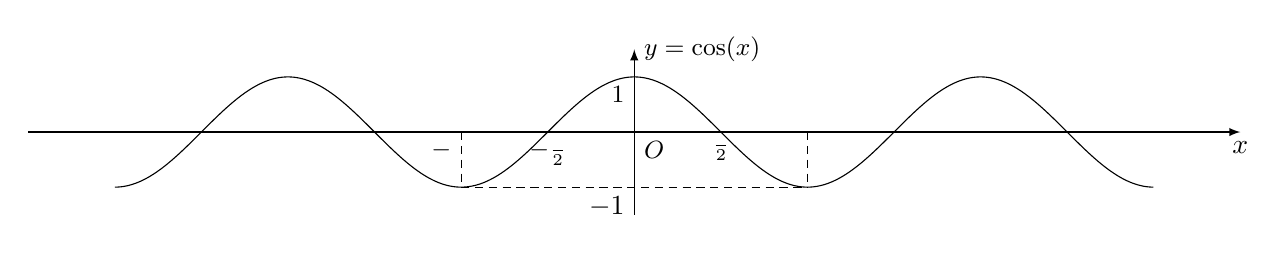
\begin{tikzpicture}[scale=0.7]
          \coordinate[label=below right:\small$O$] (O) at(0,0);
          \coordinate[label=below :\small $\frac{\piup}{2}$] (t1) at(pi/2,0);
          \coordinate[label=below :\small $-\frac{\piup}{2}$] (t2) at(-pi/2,0);
          \coordinate[label=below left :\small $1$] (t3) at(0,1);
          \draw[->,>=latex](-3.5*pi,0)--(3.5*pi,0)node[below](x) {$x$};
          \draw[->,>=latex](0,-1.5)--(0,1.5)node[right](y) {\small $y=\cos(x)$};
          \draw [domain=-3*pi:3*pi,samples=1000] plot(\x,{cos(\x r)});
          \draw[densely dashed](pi,0)node[below left](pi){\small $\piup$}--++(0,-1);
          \draw[densely dashed](-pi,0)node[below left](-pi){\small $-\piup$}--++(0,-1);
          \draw[densely dashed](-pi,-1)--(0,-1)node[below left](min){$-1$}--++(pi,0);
        \end{tikzpicture}
      \end{center}
      \vspace{-0.7cm}
      \begin{enumerate}[label=\circled{\arabic*}]
        \item 定义域:$x\inR$;\quad 值域:$ \left[-1,1\right] $;\quad 奇偶性:偶函数;
        \item 对称轴:$ x=k\piup \left(k\inZ\right) $;\quad 对称中心:$\left(k\piup+\dfrac{\piup}{2},0\right)\left(k\inZ\right)$;\quad 最小正周期:$ T=2\piup  $;
        \item 单调递增区间:$ \left[2k\piup-\piup,2k\piup\right] \left(k\inZ\right)$;\quad
              单调递减区间:$ \left[2k\piup,2k\piup+\piup\right]\left(k\inZ\right) $.
      \end{enumerate}
    \subsubsection{正切函数}
      \vspace{-0.5cm}
      \begin{center}
        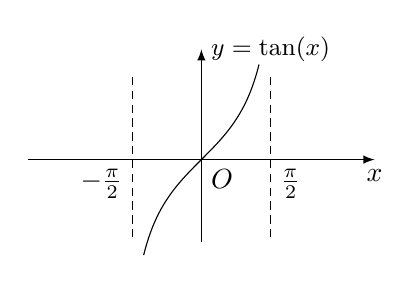
\begin{tikzpicture}[scale=0.7]
          \coordinate[label=below right:$O$] (O) at(0,0);
          %\coordinate[label=below :$\dfrac{\pi}{2}$] (t1) at(pi/2,0);
          %\coordinate[label=below :$2\pi$] (t2) at(2*pi,0);
          \draw[->,>=latex](-pi,0)--(pi,0)node[below](x) {$x$};
          \draw[->,>=latex](0,-1.5)--(0,2)node[right](y) {\small $y=\tan(x)$};
          \draw [domain=-pi/3:1/3*pi,samples=1000] plot(\x,{tan(\x r)});
          \draw[densely dashed](2*pi/5,1.5)--++(0,-1.5)node[below right](pi){$\frac{\pi}{2}$}--++(0,-1.5);
          \draw[densely dashed](-2*pi/5,1.5)--++(0,-1.5)node[below left](pi){$-\frac{\pi}{2}$}--++(0,-1.5);
        \end{tikzpicture}
      \end{center}
      \vspace{-0.7cm}
      \begin{enumerate}[label=\circled{\arabic*}]
        \item 定义域:$\Bigl\{x\Bigm|x\ne k\piup+\dfrac{\piup}2,k\inZ\Bigr\}$;\quad 值域:$ \mathbf{R} $;\quad 奇偶性:奇函数;
        \item 对称中心:$\left(\dfrac{k\piup}2,0\right)\left(k\inZ\right)$;\quad 最小正周期:$ T=\piup  $;
        \item 单调递增区间:$ \left(k\piup-\dfrac{\piup}{2},k\piup+\dfrac{\piup}{2}\right) \left(k\inZ\right)$;
        \end{enumerate}
    \begin{exercise}
      \item%福州一中学2016-2017学年高一下学期期末考试数学…….doc-1【三角函数,比大小】
        (2017 \textbullet {\kaishu 福州一中} 1)
        设$a=\sin36\degree$,$b=\cos(-52\degree)$,$c=\tan218\degree$,则\xz
        \xx{$a<b<c$}
         {$a<c<b$}
         {$b<c<a$}
         {$b<a<c$}
        \begin{answer}
          A
        \end{answer}
      \item%《2018天利38套:高考真题单元专题训练(理)ISBN978-7-223-03393-0》专题14三角函数的图像与性质P53p4【2017•全国新课标】【正弦曲线性质】
          {\kaishu (2017 \textbullet 全国新课标)}
          设函数$f(x)=\cos\Bp{x+\dfrac{\piup}3}$,则下列结论错误的是\xz
          \xx{$f(x)$的一个周期为$-2\piup$}
           {$y=f(x)$的图像关于直线$x=\dfrac{8\piup}3$对称}
           {$f(x+\piup)$的一个零点为$x=\dfrac{\piup}6$}
           {$f(x)$在$\Bp{\dfrac{\piup}2,\piup}$单调递减}
          \begin{answer}
            D
          \end{answer}
      \item%福建师大附中2016-2017高一下期末考试数学试题…….doc-14【三角函数取值范围】
        (2017 \textbullet {\kaishu 师大附中} 14)
        函数$y=\sqrt{\cos x-\dfrac12}$的定义域为\tk.
        \begin{answer}
          $\Bigl[-\dfrac{\piup}3+2k\piup,\dfrac{\piup}3+2k\piup\Bigr]$,$k\inZ$
        \end{answer}
      \item%福州第三中中学2015-2016学年高一数学第二学期期末检测.doc-7【三角函数 复合函数单调性】
        (2016 \textbullet {\kaishu 福州三中} 7)
        函数$y=\sin\Bigl(-2x+\dfrac{\piup}4 \Bigr)$的单调增区间为\xz
        \xx{$\Bigl[k\piup-\dfrac{\piup}8,k\piup+\dfrac{3\piup}8 \Bigr]$,$k\in\mathbb{Z}$}
         {$\Bigl[k\piup+\dfrac{3\piup}8,k\piup+\dfrac{7\piup}8 \Bigr]$,$k\in\mathbb{Z}$}
         {$\Bigl[k\piup-\dfrac{3\piup}8,k\piup+\dfrac{\piup}8 \Bigr]$,$k\in\mathbb{Z}$}
         {$\Bigl[k\piup+\dfrac{\piup}8,k\piup+\dfrac{5\piup}8 \Bigr]$,$k\in\mathbb{Z}$}
        \begin{answer}
          B
        \end{answer}
      \item%福州第三中中学2015-2016学年高一数学第二学期期末检测.doc-14【三角函数性质 综合判断】
        (2016 \textbullet {\kaishu 福州三中} 14)
        关于函数$f(x)=2\sin\Bp{2x+\dfrac{\piup}3}$($x\inR$),有下列说法:\\
        \circled{1}由$f(x_1)=f(x_2)=0$可得$x_1-x_2$必是$\piup$的整数倍;
        \circled{2}$y=f(x)$的表达式可改写为$f(x)=2\cos\Bp{2x-\dfrac{\piup}6}$;
        \circled{3}$y=f(x)$的图像关于点$\Bp{-\dfrac{\piup}6,0}$对称;
        \circled{4}$y=f(x)$的图像关于直线$x=\dfrac{7\piup}{12}$对称.\\
        其中说法正确的序号是\tk.
        \begin{answer}
          \circled{2}\circled{3}\circled{4}
        \end{answer}
      \item%福建师大附中2016-2017高一下期末考试数学试题…….doc-10【三角函数取值范围,方程解】
        (2017 \textbullet {\kaishu 师大附中} 10)
        若方程$\cos\Bp{2x+\dfracp{}4}=m$在区间$\Bigl[0,\dfracp{}2\Bigr]$上有两个实根,则实数$m$取值范围是\xz
        \xx{$\Bigl[-1,-\dfrac{\sqrt2}2\Bigr]$}
         {$\Bigl(-1,-\dfrac{\sqrt2}2\Bigr]$}
         {$\Bigl[\dfrac{\sqrt2}2,1\Bigr]$}
         {$\Bigl[\dfrac{\sqrt2}2,1\Bigr)$}
        \begin{answer}
          B
        \end{answer}
      \item%福建师大附中2015-2016学年高一数学第二学期期末检测.doc-22【三角函数性质】
        (2016 \textbullet {\kaishu 师大附中} 22)
        已知函数$f(x)=3\sin\Bp{\dfrac{x}2+\dfrac{\piup}6}+3$,$x\inR$.\\
        (I)求函数$f(x)$的单调增区间;\\
        (II)若$x\in\Bigl[\dfrac{\piup}3,\dfrac{4\piup}3\Bigr]$,求$f(x)$的最大值和最小值,
        并指出$f(x)$取得最值时相
        应$x$的值.
        \begin{answer}
          (I)$\Bigl[-\dfrac{4\piup}3+4k\piup,\dfrac{2\piup}3+4k\piup\Bigr]$,$k\inZ$;
          (II)当$x=\dfrac{4\piup}3$时,取最小值$f(x)_{\min}=\dfrac92$;当$x=\dfrac{2\piup}3$时,取最大值$f(x)_{\max}=6$.
        \end{answer}
      \vspace{5cm}
      \item%福建师大附中2015-2016学年高一数学第二学期期末检测.doc-24【三角函数 复合函数最值】
        (2016 \textbullet {\kaishu 师大附中} 24)
        求函数$f(x)=3-2a\sin x-\cos^2x$的最小值.
        \begin{answer}
          $y_{\min}=\begin{cases}
            2a+3,\quad a\leqslant-1,\\
            a^2+2,\quad -1<a<1,\\
            -2a+3,\quad a\geqslant+3.
          \end{cases}$
        \end{answer}
      \vspace{5cm}
    \end{exercise}
  \subsection{三角函数图像的(线性)变换}
    \begin{description}
      \item 函数$y=f(x)$图像经平移或伸缩变换后的图像解析式:{\kaishu 坐标变量的变化与图像相反}
        \[\begin{aligned}
          y=f(x)&\xrightarrow[\text{平移}\abs{a}\text{个单位}]{\text{向左}(a>0)\text{或向右}(a<0)}y=f(x+a)\hspace{3em}
          y=f(x)\xrightarrow[\text{纵坐标不变}]{\text{横坐标变为原来的}k\text{倍}}y=f\Bp{\dfrac{x}{k}}\\
          y=f(x)&\xrightarrow[\text{平移}\abs{a}\text{个单位}]{\text{向下}(a>0)\text{或向上}(a<0)}y+a=f(x)\hspace{3em}
          y=f(x)\xrightarrow[\text{横坐标不变}]{\text{纵坐标变为原来的}A\text{倍}}\dfrac{y}{A}=f(x)
        \end{aligned}\]
      \item 由函数$y=\sin(x)$的图象经过变换得到$y=A\sin\left(\omega x+\varphi\right)$的图象方法\\
        \begin{minipage}[h]{0.45\linewidth}
          \hspace{-2em}\circled{1} 先平移后伸缩
            \[\begin{aligned}
              y=\sin x&\xrightarrow[\text{平移}\abs{\varphi}\text{个单位}]{\text{向左}(\varphi>0)\text{或向右}(\varphi<0)}y=\sin\left(x+\varphi\right)\\
              &\xrightarrow[\text{纵坐标不变}]{\text{横坐标变为原来的}\tfrac{1}{\omega}}y=\sin\left(\omega x+\varphi\right)\\
              &\xrightarrow[\text{横坐标不变}]{\text{纵坐标变为原来的}A\text{倍}}y=A\sin\left(\omega x+\varphi\right)
            \end{aligned}\]
        \end{minipage}\hfill
        \begin{minipage}[h]{0.55\linewidth}
          \circled{2} 先伸缩后平移
            \[\begin{aligned}
              y=\sin x&\xrightarrow[\text{纵坐标不变}]{\text{横坐标变为原来的}\tfrac{1}{\omega}}y=\sin\omega x\\
              &\xrightarrow[\text{平移}\abs{\tfrac{\varphi}{\omega}}\text{个单位}]{\text{向左}(\varphi>0)\text{或向右}(\varphi<0)}y=\sin\biggl[\omega\Bp{x+\dfrac{\varphi}{\omega}}\biggr]\\
              &\xrightarrow[\text{横坐标不变}]{\text{纵坐标变为原来的}A\text{倍}}y=A\sin\left(\omega x+\varphi\right)
            \end{aligned}\]
        \end{minipage}
      \item 由图象求函数$y=A\sin\left(\omega x+\varphi\right)$的解析式一般步骤:
        \begin{enumerate}[label=\arabic*\degree]
          \item 由函数的最值确定$ A $的取值;
          \item 由函数的周期确定$ \omega $的值, 周期:$ T=\dfrac{2\pi}{\abs{\omega}} $;
          \item 由函数图象最高点(最低点)的坐标得到关于$ \varphi $的方程,再由$ \varphi $的范围确定$ \varphi $的值.
        \end{enumerate}
    \end{description}
    \begin{exercise}
      \item%《2018天利38套:高考真题单元专题训练(理)ISBN978-7-223-03393-0》专题14三角函数的图像与性质P53p4【2015•全国新课标】【正弦曲线图像】
           %LaTeX-master/sanjiaohanshu/sanjiaohanshu-gaokao.tex 4
        {\kaishu (2015 \textbullet 全国新课标)}
        函数$f(x)=\cos(\omega x+\varphi)$的部分图象如图所示,则$f(x)$的单调递减区间为\xz
        \begin{minipage}[b]{0.8\linewidth}
          \vspace{2.5em}
          \xx{$\Bigl(k\piup-\dfrac{1}{4},k\piup+\dfrac{3}{4}\Bigr),k\in\mathbb{Z}$}
            {$ \Bigl(2k\piup-\dfrac{1}{4},2k\piup+\dfrac{3}{4}\Bigr),k\in\mathbb{Z}$}
            {$ \Bigl(k-\dfrac{1}{4},k+\dfrac{3}{4}\Bigr),k\in\mathbb{Z}$}
            {$\Bigl(2k-\dfrac{1}{4},2k+\dfrac{3}{4}\Bigr),k\in\mathbb{Z} $}
        \end{minipage}\hfill
        \begin{minipage}[h]{0.2\linewidth}
          \vspace{-3cm}
          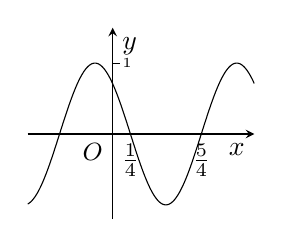
\begin{tikzpicture}[scale=0.9]
            \node[below left](O) at(0,0) {\small$\bm{O}$};
            \draw(0,1)node[right]{\tiny$1$}--(0.1,1);
            \clip(-1.2,-1.2) rectangle (2,1.5);
            \draw[->,>=stealth](-1.2,0)--(2,0) node[below left] (x){$x$};
            \draw[->,>=stealth](0,-1.2)--(0,1.5) node[below right] (y){$y$};
            \draw[domain=-1.2:2,samples=1000] plot(\x,{cos((pi*(\x)+1/4*pi) r)});
            \node[below] (A)at (0.25,0){$\frac{1}{4}$};
            \node[below] (B)at (1.25,0){$\frac{5}{4}$};
          \end{tikzpicture}
        \end{minipage}
        \begin{answer}
          D
        \end{answer}
      \item%福州三中中学2015-2016学年高一数学第二学期期末检测.docx-9【正弦曲线图像】
        (2016 \textbullet {\kaishu 福州三中} 9)
        将函数$y=\sin\Bigl(x-\dfrac{\piup}3\Bigr)$的图像上所有点的横坐标伸长到原来的2倍(纵坐标不变),再将所得的图像向左平移$\dfrac{\piup}3$个单位,得到的函数图像对应的解析式是\xz
        \xx{$y=\sin\dfrac x2$}
          {$y=\sin\Bigl(\dfrac x2-\dfrac{\piup}2\Bigr)$}
          {$y=\sin\Bigl(\dfrac{x}2-\dfrac{\piup}6\Bigr)$}
          {$y=\sin\Bigl(2x-\dfrac{\piup}6\Bigr)$}
        \begin{answer}
          C
        \end{answer}
      \item%福州一中2015-2016学年高一数学第二学期期末检测.docx-5【正弦曲线图像】
        (2016 \textbullet {\kaishu 福州一中} 5)
        函数$y=\sin\Bp{2x+\dfracp{}3}$的图像向右平移$\dfrac{\piup}6$个单位,所得的图像对应的函数\xz
        \xx{为非奇非偶函数}
         {图像的对称中心为$(2k\piup,0)$($k\inZ$)}
         {为奇函数}
         {在$\Bigl[-\dfrac{\piup}3,\dfrac{\piup}6\Bigr]$上单调递增}
        \begin{answer}
          C
        \end{answer}
      \item%福州屏东中学2016-2017学年高一下学期期末考试数学试题.doc-10【正弦曲线图像】
        (2017 \textbullet {\kaishu 屏东中学} 10)
        函数$f(x)=\sin(\omega x+\phi)$(其中$\abs{\phi}<\dfrac{\piup}2$)的图像如图所示,为了得到$y=\sin\omega x$的图像,只需把$y=f(x)$的图像上所有点(\hspace{2.5em})个长度单位.\\
        \begin{minipage}[b]{0.8\linewidth}
          \vspace{2.5em}
          \xx{向右平移$\dfrac{\piup}6$}
           {向右平移$\dfrac{\piup}{12}$}
           {向左平移$\dfrac{\piup}6$}
           {向左平移$\dfrac{\piup}{12}$}
        \end{minipage}\hfill
        \begin{minipage}[h]{0.2\linewidth}
          \vspace{-2.7cm}
          \begin{center}
            \begin{tikzpicture}[scale=0.8]
              \coordinate[label=below left:$O$] (O) at(0,0);
              \coordinate[label=above :\small$\tfrac{\piup}3$] (t1) at(pi/3,0);
              \draw[->,>=latex](-0.2*pi,0)--(1.2*pi,0)node[below](x) {$x$};
              \draw[->,>=latex](0,-1.5)--(0,1.5)node[right](y) {\small $y$};
              \draw [domain=-0.1*pi:0.9*pi,samples=100] plot(\x,{sin((2*\x+pi/3) r)});
              \draw[densely dashed](7*pi/12,0)node[above](pi){$\tfrac{7\piup}{12}$}--++(0,-1);
              \draw[densely dashed](0,-1)node[left](min){$-1$}--++(7*pi/12,0);
            \end{tikzpicture}
          \end{center}
        \end{minipage}
         \begin{answer}
           A
         \end{answer}
        \vspace{-0.9cm}
      \item%《2018天利38套:高考真题单元专题训练(理)ISBN978-7-223-03393-0》专题14三角函数的图像与性质P53p8【2017•天津】【正弦曲线解析式】
            {\kaishu (2017 \textbullet 天津)}
            设函数$f(x)=2\sin(\omega x+\varphi)$,$x\inR$,其中$\omega>0$,$\abs{\varphi}<\piup$,若$f\Bp{\dfrac{5\piup}8}=2$,$f\Bp{\dfrac{11\piup}8}=0$,且$f(x)$的最小正周期大于$\piup$,则\xz
            \xx{$\omega=\dfrac23$,$\varphi=\dfrac{\piup}{12}$}
             {$\omega=\dfrac23$,$\varphi=-\dfrac{11\piup}{12}$}
             {$\omega=\dfrac13$,$\varphi=-\dfrac{11\piup}{24}$}
             {$\omega=\dfrac13$,$\varphi=\dfrac{7\piup}{24}$}
            \begin{answer}
              A
            \end{answer}
      \newpage
      % \item%高中数学习题解法辞典.pdf 2-2-1
      %   已知函数$f(x)=A\sin(\omega x+\varphi)(A,\omega,\varphi\text{为常数},\omega>0)$的图像上相邻两个最高点的坐标分别是$\Bigl(\dfrac{\piup}{12},2\Bigr)$,$\Bigl(\dfrac{13\piup}{12},2\Bigr)$.\\
      %   (1) 求函数$f(x)$的一个表达式;\\
      %   (2)画出函数$f(x)$在长度为一个周期的闭区间上的简图;\\
      %   (3)说明经过怎样的变换,可以由$y=\sin x$的图像得到$y=f(x)$的图像.
      %   \begin{answer}
      %     (1)$y=2\sin\Bigl(2x+\dfrac{\piup}3\Bigr)(\varphi=k\piup-\dfrac{2\piup}3$即可);(2)略;(3)将$y=\sin x$图像上所有点向左平移$\dfrac{\piup}3$个单位得到$y=\sin \Bigl(x+\dfrac{\piup}3\Bigr)$的图像;再把$y=\sin \Bigl(x+\dfrac{\piup}3\Bigr)$的图像上所有点的横坐标缩短到原来的$\dfrac12$(纵坐标不变),得到$y=\sin \Bigl(2x+\dfrac{\piup}3\Bigr)$的图像;最后把$y=\sin \Bigl(2x+\dfrac{\piup}3\Bigr)$的图像上所有点的纵坐标伸长到原来的2倍(横坐标不变),即可得到函数$y=f(x)$的图像.
      %   \end{answer}
      \item%《2018天利38套:高考真题单元专题训练(理)ISBN978-7-223-03393-0》专题14三角函数的图像与性质P54p18【2017•山东】【正弦曲线解析式,三角恒等变换】
            {\kaishu (2017 \textbullet 山东)}
            设函数$f(x)=\sin\Bp{\omega x-\dfrac{\piup}6}+\sin\Bp{\omega x-\dfrac{\piup}2}$,其中$0<\omega<3$.已知$f\Bp{\dfrac{\piup}6}=0$.\\
            (I)求$\omega$;\\
            (II)将函数$y=f(x)$的图像上各点的横坐标伸长为原来的2倍(纵坐标不变),再将得到的图像向左平移$\dfrac{\piup}4$个单位,得到函数$y=g(x)$的图像,求$g(x)$在$\Bigl[-\dfrac{\piup}4,\dfrac{3\piup}4\Bigr]$上的最小值.
            \begin{answer}
              (I)$f(x)=\sqrt3\sin\Bp{\omega x-\dfrac{\piup}3}$,$\omega=2$.
              (II)$g(x)=\sqrt3\sin\Bp{x-\dfrac{\piup}{12}}$,当$x=-\dfrac{\piup}4$时,$g(x)$取得最小值$-\dfrac32$
            \end{answer}
      \vspace{5cm}
    \end{exercise}

\section{课后作业}
  \begin{exercise}
    \item%福州屏东中学2016-2017学年高一下学期期末考试数学试题.doc-11【扇形面积】
      (2017 \textbullet {\kaishu 屏东中学} 11)
      若一个扇形的周长与面积的数值相等,则该扇形所在圆的半径不可能等于\xz
      \xx{5}{2}{3}{4}
      \begin{answer}
        B
      \end{answer}
    \item%《2018天利38套:高考真题单元专题训练(文)》专题13三角函数的概念……P41p5【2009文•重庆】【三角函数 比大小】
      {\kaishu (2009文 \textbullet 重庆)}
      %福建师大附中2015-2016学年高一数学第二学期期末检测.doc-8【三角函数 比大小】
      (2016 \textbullet {\kaishu 师大附中} 8)
      下列关系式中正确的是\xz
      \xx{$\sin11\degree<\cos10\degree<\sin168\degree$}
       {$\sin168\degree\sin11\degree<\cos10\degree$}
       {$\sin11\degree<\sin168\degree<\cos10\degree$}
       {$\sin168\degree<\cos10\degree<\sin11\degree$}
      \begin{answer}
        C
      \end{answer}
    \item%福州屏东中学2016-2017学年高一下学期期末考试数学试题.doc-9【三角函数取值范围】
      (2017 \textbullet {\kaishu 屏东中学} 9)
      函数$y=\sqrt{2\cos x+1}$的定义域是\xz
      \xx{$\Bigl[2k\piup-\dfrac{\piup}3,2k\piup+\dfrac{\piup}3 \Bigr]$,$k\in\mathbb{Z}$}
       {$\Bigl[2k\piup-\dfrac{\piup}6,2k\piup+\dfrac{\piup}6 \Bigr]$,$k\in\mathbb{Z}$}
       {$\Bigl[2k\piup+\dfrac{\piup}3,2k\piup+\dfrac{2\piup}3 \Bigr]$,$k\in\mathbb{Z}$}
       {$\Bigl[2k\piup-\dfrac{2\piup}3,2k\piup+\dfrac{2\piup}3 \Bigr]$,$k\in\mathbb{Z}$}
      \begin{answer}
        D
      \end{answer}
    \item%福建师大附中2015-2016学年高一数学第二学期期末检测(实验班).doc-6【三角函数变换、诱导公式】
      (2016 \textbullet {\kaishu 师大附中实验班} 6)
      已知函数$f(x)=\sin(\omega x+\phi)$(其中$\abs{\phi}<\dfrac{\piup}2$)图像相邻对称轴的距离为$\dfrac{\piup}2$,一个对称中心为$\Bp{-\dfrac{\piup}6}$,为了得到$y=\cos\omega x$的图像,则只要将$y=f(x)$的图像\xz\\
      \xx{向右平移$\dfrac{\piup}6$个单位}
       {向右平移$\dfrac{\piup}{12}$个单位}
       {向左平移$\dfrac{\piup}6$个单位}
       {向左平移$\dfrac{\piup}{12}$个单位}
      \begin{answer}
        D
      \end{answer}
    \item%福州一中学2016-2017学年高一下学期期末考试数学…….doc-10【三角函数与二次函数复合值域,同名三角函数关系】【中上难度】
      (2017 \textbullet {\kaishu 福州一中} 10)
      关于$x$的方程$\sin x-\cos^2x+a=0$在$x\in[0,2\piup)$内恰有4解,则实数$a$的取值范围是\xz
      \xx{$\Bp{-1,\dfrac54}$}
       {$\Bp{1,\dfrac54}$}
       {$\Bigl[-1,\dfrac54\Bigr)$}
       {$\Bigl[1,\dfrac54\Bigr)$}
      \begin{answer}
        B
      \end{answer}
    %填空题
    \item%福建师大附中2015-2016学年高一数学第二学期期末检测.doc-17【诱导公式】
      (2016 \textbullet {\kaishu 师大附中} 17)
      已知$\sin\Bp{\theta-\dfracp{}4}=\dfrac13$,则$\cos\Bp{\dfracp{}4+\theta}$的值等于\tk.
      \begin{answer}
        $-\dfrac13$
      \end{answer}
    %暂用
    \item%《习题化知识清单》P73易混清单例
      函数$y=2\sin\Bigl(\dfrac{\piup}3-2x \Bigr)$的单调增区间为\tk.
      \begin{answer}
        $\Bigl[k\piup+\dfrac{5\piup}{12},k\piup+\dfrac{11\piup}{12} \Bigr],k\in\mathbb{Z}$
      \end{answer}
    % \item%函数y=Asin(ωx+φ)的图象及简单应用P11.14
    %   已知曲线$y=A\sin(\omega x+\varphi)$$(A>0,\omega>0,\abs{\varphi}\leqslant\dfrac{\piup}2)$上最高点为$(2,\sqrt{2})$,该最高点与相邻的最低点间的曲线与$x$轴交于点$(6,0)$.\\
    %   (1)该函数的解析式;\\
    %   (2)该函数在$x\in[-6,0]$上的值域.
    %   \begin{answer}
    %     (1)$y=\sqrt{2}\sin\Bigl(\dfrac{\piup}8x+\dfrac{\piup}4\Bigr)$;
    %     (2)$[-\sqrt{2},0]$
    %   \end{answer}
    % \vspace{5cm}
    \item%福州屏东中学2016-2017学年高一下学期期末考试数学试题.doc-20【正弦曲线图像】
      (2017 \textbullet {\kaishu 屏东中学} 20)
      已知角$\alpha$的终边过点$P(-3,4)$.\\
      (1)求$\dfrac{\tan\alpha}{\sin(\piup-\alpha)-\cos\Bp{\dfracp12+\alpha}}$的值;\quad
      (2)若$\beta$为第三象限角,且$\tan\beta=\dfrac34$,求$\cos(2\alpha-\beta)$的值.
      \begin{answer}
        (1)$-\dfrac56$;
        (2)$\dfrac45$.
      \end{answer}
    \vspace{3cm}
    \item%《2018天利38套:高考真题单元专题训练(理)ISBN978-7-223-03438-8》专题15三角恒等变换 P59p20【2014•广东】
      (2014 \textbullet {\kaishu 广东})已知函数$f(x)=A\sin{\Bigl(x+\dfrac{\piup}4\Bigr)}$,$x\in\mathbb{R}$,且$f\Bigl(\dfrac{5\piup}{12}\Bigr)=\dfrac{3}2$.\\
      (I)求$A$的值;\\
      (II)若$f(\theta)+f(-\theta)=\dfrac{3}2$,$\theta\in \Bigl(0,\dfrac{\piup}2\Bigr)$,求$f\Bigl(\dfrac{3\piup}4-\theta\Bigr)$.
      \begin{answer}
        (I)$A=\sqrt{3}$;
        (II)$f\Bigl(\dfrac{3\piup}4-\theta\Bigr)=\dfrac{\sqrt{30}}4$
      \end{answer}
    \vspace{4cm}
    % \item%福州格致中学2015-2016学年高一数学第二学期期末检测.docx-22
    %   % (附加题:本小题满分15分)\\
    %   % (福州格致中学2015-2016学年高一数学第二学期期末检测22)
    %   (2016 \textbullet {\kaishu 格致中学} 22)
    %   已知函数$f(x)=A\sin(\omega x+\varphi)+B (A>0,\omega>0)$的一系列对应值如下表:
    %   \begin{center}
    %     \renewcommand{\arraystretch}{1.4}
    %     \begin{tabular}{|*{8}{c|}}
    %       \hline
    %         $x$
    %         &$\dfrac{\piup}6$
    %         &$-\dfrac{\piup}3$
    %         &$-\dfrac{5\piup}6$
    %         &$-\dfrac{4\piup}3$
    %         &$-\dfrac{11\piup}6$
    %         &$-\dfrac{7\piup}3$
    %         &$-\dfrac{17\piup}6$\\
    %       \hline
    %         $y$
    %         &$-1$
    %         &$1$
    %         &$3$
    %         &$1$
    %         &$-1$
    %         &$1$
    %         &$3$\\
    %       \hline
    %     \end{tabular}\\
    %   \end{center}
    %   (1)根据表格提供的数据求函数$f(x)$的一个解析式;\\
    %   (2)根据(1)的结果:\\
    %   \;(i)当$x\in\Bigl[0,\dfrac{\piup}3\Bigr]$时,方程$f(3x)=m$恰有两个不同的解,求实数$m$的取值范围;\\
    %   \;(ii)若是$\alpha,\beta$是锐角三角形的两个内角,试比较$f(\sin \alpha)$与$f(\cos \beta)$的大小.
    %   \begin{answer}
    %     (1)$f(x)=2\sin\Bigl(x-\dfrac{\piup}3\Bigr)+1$;(2)(i)$[\sqrt{3}+1,3)$;(ii)易得$f(x)$在$[-\dfrac{\piup}6,\dfrac{5\piup}6]$上单调递增,故$f(x)$在$[0,1]$上单调递增;又$0<\dfrac{\piup}2-\beta<\alpha<\dfrac{\piup}2$,从而$\sin\alpha>\sin(\dfrac{\piup}2-\beta)=\cos\beta$,于是$f(\sin \alpha)>f(\cos \beta)$
    %   \end{answer}
    \item%福州一中学2016-2017学年高一下学期期末考试数学…….doc-10【正弦曲线图像】
      \begin{minipage}[t]{0.7\linewidth}
        (2017 \textbullet {\kaishu 福州一中} 16)
        已知函数$f(x)=A\sin(\omega x+\phi)$($A>0$,$\omega>0$,$\abs{\phi}<\dfrac{\piup}2$)的部分图像如图所示,\\
        (I)求函数$f(x)$的单调递增区间;\\
        (II)将$f(x)$的图像向右平移$\dfrac{\piup}3$个单位长度,再将所得的图像上各点的横坐标缩短到原来的$\dfrac12$倍(纵坐标不变),
        得到$g(x)$的图像;当$x\in\Bp{0,\dfrac{\piup}4}$时,求$g(x)$的值域.
      \end{minipage}\hfill
      \begin{minipage}[h]{0.3\linewidth}
        \vspace{2.7cm}
        \begin{center}
          \begin{tikzpicture}[scale=0.8]
            \coordinate[label=below left:$O$] (O) at(0,0);
            \coordinate[label=above :\small$\tfrac{\piup}3$] (t1) at(pi/3,0);
            \draw[->,>=latex](-0.2*pi,0)--(1.2*pi,0)node[below](x) {$x$};
            \draw[->,>=latex](0,-1.5)--(0,1.5)node[right](y) {\small $y$};
            \draw [domain=-0.1*pi:0.9*pi,samples=100] plot(\x,{sin((2*\x+pi/3) r)});
            \draw[densely dashed](7*pi/12,0)node[above](pi){$\tfrac{7\piup}{12}$}--++(0,-1);
            \draw[densely dashed](0,-1)node[left](min){$-\sqrt2$}--++(7*pi/12,0);
          \end{tikzpicture}
        \end{center}
      \end{minipage}
      \begin{answer}
        (I)$f(x)=\sqrt2\sin\Bp{2x+\dfrac{\piup}3}$,单调递增区间为$\Bigl[-\dfrac{5\piup}{12}+k\piup,\dfrac{\piup}{12}+k\piup\Bigr]$,$k\inZ$.
        (II)$g(x)=\sqrt2\sin\Bp{4x-\dfrac{\piup}3}$,值域:$\Bigl[-\dfrac{\sqrt6}2,\sqrt2\Bigr]$
      \end{answer}
    \vspace{4cm}

  \end{exercise}

% \section{三角恒等变换}
%   \begin{exercise}
%     \item%福州第三中中学2015-2016学年高一数学第二学期期末检测.doc-15【诱导公式,和角】
%     (2016 \textbullet {\kaishu 福州三中} 15)
%     已知$\sin\BP{\alpha+\dfrac{\piup}4}=-\dfrac35$,且$0<\alpha<\dfrac{5\piup}4$,求$\cos\BP{\alpha+\dfrac{\piup}2}$的值.
%     \begin{answer}
%       $-\dfrac{\sqrt2}{10}$
%     \end{answer}
%     \vspace{5cm}
%     \item%福州三中2017高一下数学期末卷…….doc-15【辅助角公式灵活应用】
%          %《2018天利38套:高考真题单元专题训练(理)ISBN978-7-223-03438-8》专题14三角函数的图像与性质 P54p16【2013•全国新课标】
%       (2017 \textbullet {\kaishu 福州三中} 15)(2013 \textbullet {\kaishu 全国新课标})
%       设当$x=\theta$时,函数$f(x)=\sin x-2\cos x$取得最大值,则$\cos\theta=$\tk.
%       \begin{answer}
%         $-\dfrac{2\sqrt{5}}5$
%       \end{answer}
%     \item%《2018天利38套:高考真题单元专题训练(理)ISBN978-7-223-03393-0》专题14三角函数的图像与性质P54p13【2016•全国新课标】【三角函数变换、辅助角】
%         {\kaishu (2016 \textbullet 全国新课标)}
%         函数$y=\sin x-\sqrt3\cos x$的图像可由函数$y=\sin x+\sqrt3\cos x$的图像至少向右平移\tk个单位长度得到.
%         \begin{answer}
%           $\dfrac{2\piup}3$
%         \end{answer}
%     \item%福建师大附中2016-2017高一下期末考试数学试题…….doc-9【二倍角、诱导公式】
%      (2017 \textbullet {\kaishu 师大附中} 9)
%      已知$\sin\Bp{\dfracp{}6-\alpha}=\dfrac13$,则$\cos\Bp{\dfracp{2}3+2\alpha}=$\xz
%      \xx{$-\dfrac79$}
%       {$-\dfrac13$}
%       {$\dfrac13$}
%       {$\dfrac79$}
%      \begin{answer}
%        A
%      \end{answer}
%     \item%福州三中2017高一下数学期末卷…….doc-6【二倍角、诱导公式】
%       (2017 \textbullet {\kaishu 福州三中} 6)
%       已知$\sin\Bp{\dfracp{3}2+\theta}+2\cos(\piup+\theta)=\sin(-\theta)$,则$\sin\theta\cos\theta+\cos^2\theta=$\xz
%       \xx{$-\dfrac15$}
%        {$\dfrac25$}
%        {$\dfrac35$}
%        {$1$}
%       \begin{answer}
%         B
%       \end{answer}
%     \item%福州一中学2016-2017学年高一下学期期末考试数学…….doc-7【和角公式,韦达定理】
%       (2017 \textbullet {\kaishu 福州一中} 7)
%       已知$\tan\alpha$,$\tan\beta$是方程$x^2+3\sqrt3x+4=0$的两根,$\alpha,\beta\in(0,\piup)$,则$\alpha+\beta=$\xz
%       \xx{$\dfracp{}3$}
%        {$\dfracp{2}3$}
%        {$\dfracp{4}3$}
%        {$\dfracp{}3$或$\dfracp{4}3$}
%       \begin{answer}
%         A
%       \end{answer}
%     \item%福州一中学2016-2017学年高一下学期期末考试数学…….doc-5【二倍角、半角、奇偶性、周期性】
%         (2017 \textbullet {\kaishu 福州一中} 5)
%         函数$f(x)=\dfrac12(1-\cos{2x})\cos^2x$,$x\in\mathbb{R}$是\xz
%         \xx{最小正周期为$\piup$的偶函数}
%          {最小正周期为$\dfracp{}2$的偶函数}
%          {最小正周期为$\piup$的奇函数}
%          {最小正周期为$\dfracp{}2$的奇函数}
%         \begin{answer}
%           B
%         \end{answer}
%     \item%福州三中2017高一下数学期末卷…….doc-17【三角函数化简、二倍角、诱导公式】
%         (2017 \textbullet {\kaishu 福州三中} 17)
%         已知$f(x)=2\tan x+\dfrac{1-2\sin^2{\dfrac{x}2}}{\sin\dfrac{x}2\cdot\cos\dfrac{x}2}$.\\
%         (I)求$f(\dfrac{\piup}6)$的值;\\
%         (II)若$f(\alpha)=5$,求$f\Bp{\alpha+\dfrac{\piup}4}$的值.
%         \begin{answer}
%           (I)$\dfrac{8\sqrt3}3$;
%           (II)$\pm\dfrac{20}3$.
%         \end{answer}
%     \vspace{5cm}
%   \end{exercise}
% \item%福建师大附中2016-2017高一下期末考试数学试题…….doc-20【三角函数性质,向量数量积计算】
%   (2017 \textbullet {\kaishu 师大附中} 20)
%   已知向量$\bm a=(\cos x,\sin x)$,$\bm b=(3,-\sqrt3)$,记$f(x)=\bm a\cdot\bm b$.\\
%   (I)求$f(x)$的单调增区间;\\
%   (II)若$x\in[0,\piup]$,求$f(x)$的值域.
%   \begin{answer}
%     (I)$\Bigl[-\dfrac{5\piup}6+2k\piup,\dfrac{11\piup}6+2k\piup\Bigr]$,$k\inZ$;
%     (II)$[-2\sqrt3,3]$.
%   \end{answer}
% \vspace{5cm}
% \section{平面向量}
% \section{要点归纳}
%
%   \subsection{五种常见向量}
%     \begin{enumerate}[label=\arabic*)]
%       \item 单位向量:模为1的向量.
%       \item 零向量:模为0的向量.
%       \item 平行(共线向量):方向相同或相反或其一为零向量的两个向量.
%       \item 相等向量:模相等,方向相同的向量.
%       \item 相反向量:模相等,方向相反的向量.
%     \end{enumerate}
%   \subsection{平面向量运算律}
%     \begin{enumerate}[label=\arabic*)]
%       \item 交换律:
%         $\bm a+\bm b=\bm b+\bm a$,\quad
%         $\bm a\cdot\bm b=\bm b\cdot\bm a$
%       \item 结合律:
%         $(\bm{a}+\bm{b})+\bm{c}=\bm{a}+(\bm{b}+\bm{c})$,\quad
%         $(\lambda \bm a)\cdot\bm{b}=\lambda(\bm a\cdot\bm b)=\bm{a}\cdot(\lambda\bm{b})$
%       \item 分配律:
%         $(\lambda+\mu)\bm{a}=\lambda\bm{a}+\mu\bm{a}$,\quad
%         $\lambda(\bm{a}+\bm{b})=\lambda\bm{a}+\lambda\bm{b}$,\quad
%         $(\bm a+\bm b)\cdot \bm c=\bm a\cdot\bm c+\bm b\cdot \bm c$
%       \item 重要公式:(记号$\bm a^2=\bm a\cdot\bm a$)
%         $(\bm a+\bm b)(\bm a-\bm b)=\bm a^2-\bm b^2$,\quad
%         $(\bm a\pm\bm b)^2=\bm a^2\pm2\bm a\cdot\bm b+\bm b^2$.
%     \end{enumerate}
%   \subsection{两个重要定理}
%     \begin{enumerate}[label=\arabic*)]
%       \item 向量共线定理:
%         向量$\bm{a}~(\bm{a}\ne\bm{0})$与向量$\bm{b}$共线,当且仅当存在唯一的实数$ \lambda $,使得$\bm{b}=\lambda\bm{a}$.\\
%         {\kaishu
%          证明三点共线的方法:\circled{1}$\vv{AB}=\lambda\vv{AC}$,则$A$,$B$,$C$三点共线;\circled{2}$\vv{OA}=\lambda\vv{OB}+\mu\vv{OC}$,若$\lambda+\mu=1$,则$A$,$B$,$C$三点共线.
%         }
%       \item 平面向量基本定理:
%         如果$ \bm{e}_1,\bm{e}_2 $是同一平面内的两个\CJKunderdot{不共线}的向量,
%         则那么对于这一平面内的任意向量$ \bm{a} $,有且只有一对实数$ \lambda_1,~\lambda_2 $,使$\bm{a}=\lambda_1\bm{e}_1+\lambda_2\bm{e}_2$.
%         其中,不共线的向量$\bm{e}_1, \bm{e}_2$叫做表示这一平面内所有向量的一组\CJKunderdot{基底}.\\
%         {\kaishu 平面向量基本定理应用技巧:
%           \begin{enumerate}[label=\circled{\arabic*}]
%             \item 构造某一向量在同一基底下的两种不同表达形式,
%               根据向量分解的唯一性求解.即:\\
%               {\kaishu 以$\bm e_1$,$\bm e_2$为基底,且$\bm a=x_1\bm e_1+y_1\bm e_2=x_2\bm e_1+y_2\bm e_2$,则$\begin{cases}x_1=x_2\\y_1=y_2\end{cases}$}
%             \item 构造两个共线向量在同一基底下的表达形式,
%               根据向量共线定理求解.即:\\
%               {\kaishu 以$\bm e_1$,$\bm e_2$为基底,且$\bm a=x_1\bm e_1+y_1\bm e_2$,$\bm b=x_2\bm e_1+y_2\bm e_2$,且$\bm a\varparallel\bm b$,则$x_1y_2-x_2y_1=0$}
%             \item 将题目中的已知条件转化成
%               $\lambda_1\bm e_1+\lambda_2\bm e_2=\bm 0$的形式($\bm e_1$,$\bm e_2$不共线),根据$\lambda_1=\lambda_2=0$求解.
%           \end{enumerate}}
%     \end{enumerate}
%   \subsection{平面向量平行、垂直的等价条件}
%     设$\bm a=(x_1,y_1)$,$\bm b=(x_2,y_2)$,则:
%     \begin{enumerate}[label=\arabic*)]
%       \item $\bm a\varparallel\bm b$$\Leftrightarrow$$x_1y_2-x_2y_1=0$.
%       \item $\bm a\perp\bm b$
%             $\Leftrightarrow$$\bm a\cdot\bm b=0$
%             $\Leftrightarrow$$x_1x_2+y_1y_2=0$.
%     \end{enumerate}
%   \subsection{平面向量数量积相关量求解}
%     \begin{enumerate}[label=\arabic*)]
%       \item 向量夹角:设$\bm a=(x_1,y_1)$,$\bm b=(x_2,y_2)$,则
%         $\cos\vangle{\bm a}{\bm b}=\dfrac{\bm{a}\bm{\cdot}\bm{b}}{\abs{\bm{a}}\abs{\bm{b}}}=\dfrac{x_1x_2+y_1y_2}{\sqrt{x_1^2+y_1^2}\sqrt{x_2^2+y_2^2}} \quad \left(\vangle{\bm a}{\bm b}\in\left[0,\piup\right]\right)$
%       \item 向量模长:若$\bm a=(x,y)$,则$\abs{\bm a}=\sqrt{\bm a\cdot\bm a}=\sqrt{x^2+y^2}$
%       \item 向量投影:向量$\bm a$在$\bm b$方向上的投影为  $\abs{\bm{a}}\cos\theta=\dfrac{\bm a\cdot\bm b}{\abs{\bm b}}$
%     \end{enumerate}
% \begin{exercise}{\textbf{习题}}
%   \item%【向量的线性运算】
%     (2017 \textbullet {\kaishu 广东深圳二模})如图所示,正方形$ABCD$中,$M$是$BC$的中点,若$\vv{AC}=\lambda\vv{AM}+\mu\vv{BD}$,则$\lambda+\mu$等于\xz
%     \xx{$\dfrac{4}3$}
%      {$\dfrac{5}3$}
%      {$\dfrac{15}8$}
%      {$2$}
%     \begin{center}
%       \begin{tikzpicture}
%         \coordinate[label=left:$A$](A)at(0,0);
%         \coordinate[label=right:$B$](B)at(3.5,0);
%         \coordinate[label=left:$D$](D)at(0,3.5);
%         \coordinate[label=right:$C$](C)at(3.5,3.5);
%         \coordinate[label=right:$M$](M)at($(B)!0.5!(C)$);
%         \draw (A)--(B)--(C)--(D)--cycle;
%         \draw[->,>=latex] (A)--(C);
%         \draw[->,>=latex] (A)--(M);
%         \draw[->,>=latex] (B)--(D);
%       \end{tikzpicture}
%     \end{center}
%     \begin{answer}
%       B
%     \end{answer}
%   \item%福州一中学2016-2017学年高一下学期期末考试数学…….doc-3【向量共线】
%     (2017 \textbullet {\kaishu 福州一中} 3)
%     已知向量$\bm a$,$\bm b$不共线,且$\bm c=\lambda\bm a+\bm b$,$\bm d=\bm a+(2\lambda-1)\bm b$,若$\bm c$与$\bm d$方向相反,则实数$\lambda$的值为\xz
%     \xx{$1$}
%      {$-\dfrac12$}
%      {$1$或$-\dfrac12$}
%      {$-1$或$-\dfrac12$}
%     \begin{answer}
%       B
%     \end{answer}
%   \item%福州三中2017高一下数学期末卷…….doc-5【向量投影,基底表示】
%     (2017 \textbullet {\kaishu 福州三中} 5)
%     设$\bm e_1$,$\bm e_2$为单位向量,且$\bm e_1$,$\bm e_2$的夹角为$\dfrac{\piup}3$,若$\bm a=\bm e_1-3\bm e_2$,$\bm b=\bm e_1+\bm e_2$,则向量$\bm a$在$\bm b$方向上的射影为\xz
%     \xx{$-\sqrt3$}
%      {$\sqrt3$}
%      {$-\dfrac{\sqrt{10}}5$}
%      {$\dfrac{\sqrt{10}}5$}
%     \begin{answer}
%       A
%     \end{answer}
%   \item%【向量坐标法在平面几何的应用,三角函数定义】
%     %如图,
%     半径为$\sqrt{3}$的扇形$AOB$的圆心角为120\degree,点$C$在$\arc{AB}$上,且$\angle{COB}=30\degree$,若$\vv{OC}=\lambda\vv{OA}+\mu\vv{OB}$,则$\lambda+\mu$等于\xz
%     \xx{$\sqrt{3}$}
%      {$\dfrac{\sqrt{3}}3$}
%      {$\dfrac{4\sqrt{3}}3$}
%      {$2\sqrt{3}$}
%     \begin{answer}
%       A
%     \end{answer}
%   \item%【平面向量几何应用:垂直问题】
%     直角坐标系$xOy$中,$\vv{AB}=(2,1)$,$\vv{AC}=(3,k)$,若$\triangle{ABC}$是直角三角形,则$k$的可能值个数是\xz
%     \xx{1}{2}{3}{4}
%     \begin{answer}
%       B
%     \end{answer}
%   \item%福建师大附中2016-2017高一下期末考试数学试题…….doc-6【数量积,三角形形状】
%     (2017 \textbullet {\kaishu 师大附中} 6)
%     若点$O$是$\triangle{ABC}$平面内一点,且满足$(\vv{OB}-\vv{OC})\cdot(\vv{OB}+\vv{OC}-2\vv{OA})=0$,则$\triangle{ABC}$形状为\xz
%     \xx{钝角三角形}{等腰三角形}{直角三角形}{锐角三角形}
%     \begin{answer}
%       B
%     \end{answer}
%   \item%福州三中2017高一下数学期末卷…….doc-16【向量投影,基底表示】
%     (2017 \textbullet {\kaishu 福州三中} 16)
%     已知$\bm a$,$\bm b$是平面内两个相互垂直的单位向量,若向量$\bm c$满足$(\bm a-\bm c)\cdot(\bm b-\bm c)=0$,则$|\bm c|$的最大值是\tk.
%     \begin{answer}
%       $\sqrt2$
%     \end{answer}
%   \item%%福建师大附中2016-2017高一下期末考试数学试题…….doc-15【向量夹角,线性运算模长】
%     (2017 \textbullet {\kaishu 师大附中} 15)
%     已知单位向量$\bm a$,$\bm b$的夹角为$\dfracp{}3$,那么$|\bm a-2\bm b|=$\tk.
%     \begin{answer}
%       $\sqrt3$
%     \end{answer}
%   \item%【平面向量的模与夹角】
%     已知$\triangle{ABC}$是正三角形,若$\vv{AC}-\lambda\vv{AB}$与向量$\vv{AC}$的夹角大于90\degree,则实数$\lambda$的取值范围是\tk.
%     \begin{answer}
%       $(2,+\infty)$
%     \end{answer}
%   \item%福建师大附中2016-2017高一下期末考试数学试题…….doc-17【数量积,几何】
%     (2017 \textbullet {\kaishu 师大附中} 17)
%     在$\triangle{ABC}$中,$|\vv{AD}|=|\vv{BD}|=|\vv{CD}|$,$|\vv{AB}|=3$,则$\vv{AB}\cdot\vv{AD}=$\tk.
%     \begin{answer}
%       $\dfrac92$
%     \end{answer}
%   \item%【向量坐标法在平面几何的应用,直线方程】
%     在$\mathrm{Rt}\triangle{ABC}$中,$CA=CB=2$,$M$,$N$是斜边$AB$上的两个动点,且$MN=\sqrt{2}$,则$\vv{CM}\cdot\vv{CN}$的取值范围是\tk.
%     \begin{answer}
%       $\Bigl[\dfrac{3}2,2\Bigr]$
%     \end{answer}
%   \item%福州一中学2016-2017学年高一下学期期末考试数学…….doc-14【数量积,外心】
%     (2017 \textbullet {\kaishu 福州一中} 14)
%     $\triangle{ABC}$中,$CA=4$,$CB=6$,点$O$为$\triangle{ABC}$的外心,则$\vv{CO}\cdot\vv{AB}=$\tk.
%     \begin{answer}
%       5
%     \end{answer}
%   \item%福建师大附中2016-2017高一下期末考试数学试题…….doc-19【向量共线、夹角、模长】
%     (2017 \textbullet {\kaishu 师大附中} 19)
%     已知$\bm a$,$\bm b$为两个不共线向量,$\abs{\bm a}=2$,$\abs{\bm b}=1$,$\bm c=2\bm a-\bm b$,$\bm d=\bm a+k\bm b$.\\
%     (I)若$\bm c\varparallel\bm d$,求实数$k$;\\
%     (II)若$k=-7$,且$\bm c\perp\bm d$,求$\bm a$与$\bm b$的夹角.
%     \begin{answer}
%       (I)$k=-\dfrac12$
%       (II)$\vangle{\bm a}{\bm b}=\dfrac{\piup}3$
%     \end{answer}
%   \vspace{3cm}
%   \item%福州一中学2016-2017学年高一下学期期末考试数学…….doc-15【数量积,垂直】
%     (2017 \textbullet {\kaishu 福州一中} 15)
%     已知$\bm a=(\cos\alpha,k\sin\alpha)$,$\bm b=(\cos\beta,\sin\beta)$($k>0$,$0<\alpha<\beta<\dfrac{\piup}2$),且$\bm a+\bm b$与$\bm a-\bm b$相互垂直.\\
%     (1)求$k$的值;\\
%     (2)若$\bm a\cdot\bm b=\dfrac45$且$\cos\beta=\dfrac35$,求$\sin\alpha$的值.
%     \begin{answer}
%       (1)$k=1$;
%       (2)$\sin\alpha=\dfrac7{25}$
%     \end{answer}
%     \vspace{4cm}
%   \vspace{3.5cm}
%   \item%【平面向量基本定理】
%     在$\triangle{OAB}$的边$OA$,$OB$上分别取点$M$,$N$,使得$\vv{OA}=3\vv{OM}$,$\vv{OB}=4\vv{ON}$,设线段$AN$与$BM$交于点$P$,
%     记$\vv{OA}=\bm a$,$\vv{OB}=\bm b$,用$\bm a$,$\bm b$表示向量$\vv{OP}$.
%     \begin{answer}
%       $\vv{OP}=\dfrac3{11}\bm a+\dfrac3{11}\bm b$
%     \end{answer}
%   \vspace{9cm}
%   \item%【平面向量基本定理】
%     在$\triangle{OAB}$中,$\vv{OA}=4\vv{OC}$,$\vv{OB}=2\vv{OD}$,设线段$AD$与$BC$交于点$M$,
%     记$\vv{OA}=\bm a$,$\vv{OB}=\bm b$.\\
%     (1)用$\bm a$,$\bm b$表示向量$\vv{OP}$.\\
%     (2)已知在线段$AC$上取一点$E$,在线段$BD$上取一点$F$,使$EF$过点$M$,设$\vv{OE}=p\vv{OA}$,$\vv{OF}=q\vv{OA}$,求证$\dfrac1{7p}+\dfrac3{7q}=1$
%     \begin{answer}
%       (1)$\vv{OP}=\dfrac17\bm a+\dfrac37\bm b$
%       (2)略
%     \end{answer}
%   \vspace{9cm}
% \end{exercise}

% \newpage
% \section{课后作业}
%   \begin{exercise}
%     \item%【向量的线性运算】
%       若点$D$在$\triangle{ABC}$的边$BC$上,且$\vv{CD}=4\vv{DB}=r\vv{AB}+s\vv{AC}$,则$3r+s$的值为\xz
%       \xx{$\dfrac{16}5$}
%        {$\dfrac{12}5$}
%        {$\dfrac{8}5$}
%        {$\dfrac{4}5$}
%       \begin{answer}
%         C
%       \end{answer}
%     \item%福州屏东中学2016-2017学年高一下学期期末考试数学试题.doc-4【向量共线】
%       (2017 \textbullet {\kaishu 屏东中学} 4)
%       若$A(-1,1)$,$B(1,3)$,$C(x,5)$,且$\vv{AB}=\lambda\vv{BC}$,则实数$\lambda$等于\xz
%       \xx{1}{2}{3}{4}
%       \begin{answer}
%         1
%       \end{answer}
%     \item%福建师大附中2016-2017高一下期末考试数学试题…….doc-3【向量投影,坐标表示】
%       (2017 \textbullet {\kaishu 师大附中} 3)
%       若$\bm a=(2,1)$,$\bm b=(3,4)$,则向量$\bm b$在向量$\bm a$方向上的投影为\xz
%       \xx{$2\sqrt5$}
%        {$2$}
%        {$\sqrt5$}
%        {$10$}
%       \begin{answer}
%         A
%       \end{answer}
%     \item%【向量表示】
%       设$D$为$\triangle{ABC}$所在平面内一点,$\vv{BD}=3\vv{CD}$,则\xz
%       \xx{$\vv{AD}=-\dfrac13\vv{AB}+\dfrac43\vv{AC}$}
%        {$\vv{AD}=\dfrac43\vv{AB}-\dfrac13\vv{AC}$}
%        {$\vv{AD}=\dfrac23\vv{AB}-\dfrac12\vv{AC}$}
%        {$\vv{AD}=-\dfrac12\vv{AB}+\dfrac32\vv{AC}$}
%       \begin{answer}
%         D
%       \end{answer}
%     \item%【向量夹角、模长】
%       已知$|\bm a|=1$,$\bm a\cdot\bm b=\dfrac12$,$|\bm a-\bm b|^2=1$,则$\bm a$与$\bm b$的夹角等于\xz
%       \xx{30\degree}{45\degree}{60\degree}{120\degree}
%       \begin{answer}
%         C
%       \end{answer}
%     \item%【向量共线】
%       已知向量$\bm a=(2,3)$,$\bm b=(-1,2)$,若$m\bm a+4\bm b$与$\bm a-2\bm b$共线,则$m$的值为\xz
%       \xx{$\dfrac12$}{$2$}{$-\dfrac12$}{$-2$}
%       \begin{answer}
%         D
%       \end{answer}
%     \item%【向量几何应用】
%       在平面四边形$ABCD$中,若$AC=3$,$BD=2$,则$(\vv{AB}+\vv{DC})\cdot(\vv{AC}+\vv{BD})=$\tk.
%       \begin{answer}
%         5
%       \end{answer}
%     \item%【向量垂直】
%       平面向量$\bm a=(\sqrt{3},-1)$,$\bm=\Bp{\dfrac12,\dfrac{\sqrt3}2}$,若存在不同时为0的实数$k$和$t$,使$\bm x=\bm a+(t^2-3)\bm b$,$\bm y=-k\bm a+t\bm b$,且$\bm x\perp\bm y$,试求函数关系式$k=f(t)$.
%       \begin{answer}
%         $k=f(t)=\dfrac14(t^3-3t)$
%       \end{answer}
%     \vspace{2.5cm}
%     \item%福州三中2017高一下数学期末卷…….doc-18【向量垂直,模长,共线】
%       (2017 \textbullet {\kaishu 福州三中} 18)
%       平面内的向量$\bm a=(3,2)$,$\bm b=(-1,2)$,$\bm c=(4,1)$.\\
%       (I)若$(\bm a+k\bm c)\perp(2\bm b-\bm a)$,求实数$k$的值;\\
%       (II)若向量$\bm d$满足$\bm d\varparallel\bm c$,且$\abs{\bm d}=\sqrt{34}$,求向量$\bm d$的坐标.
%       \begin{answer}
%         (I)$k=-\dfrac{11}{18}$
%         (II)$\bm d=(4\sqrt2,\sqrt2)$或$\bm d=(-4\sqrt2,-\sqrt2)$
%       \end{answer}
%     \vspace{5cm}
%     \item
%       已知点$P$是$\triangle{ABC}$内一点,且满足条件$\vv{AP}+\vv{AP}+\vv{AP}=\bm 0$,设点$Q$为$CP$的延长线与$AB$的交点,令$\vv{CP}=\bm p$,试用向量$\bm p$表示$\vv{CQ}$.
%       \begin{answer}
%         $\vv{CQ}=2\bm p$
%       \end{answer}
%     \vspace{6cm}
%     \item%《2018天利38套:高考真题单元专题训练(文)》专题18平面向量的概念与运算 P63p31【2010•江苏】
%       (2010 \textbullet {\kaishu 江苏})
%       在平面直角坐标系$xOy$中,已知点$A(-1,-2)$,$B(2,3)$,$C(-2,-1)$.\\
%       (I)求以线段$AB$,$AC$为邻边的平行四边形的两条对角线的长;\\
%       (II)设实数$t$满足$(\vv{AB}-t\vv{OC})\cdot\vv{OC}=0$,求$t$的值.
%       \begin{answer}
%         (I)两条对角线长分别为$4\sqrt2$,$2\sqrt{10}$;
%         (II)$t=-\dfrac{11}5$
%       \end{answer}
%     % \item%《2018天利38套:高考真题单元专题训练(理)ISBN978-7-223-03438-8》专题18平面向量的应用 P72p17【2014•陕西】
%     %   (2014 \textbullet {\kaishu 陕西})
%     %   在直角坐标系$xOy$中,已知点$A(1,1)$,$B(2,3)$,$C(3,2)$,点$P(x,y)$在$\triangle{ABC}$三边围成的区域(含边界)上.\\
%     %   (I)若$\vv{PA}+\vv{PB}+\vv{PC}=\bm 0$,求$\abs{\vv{OP}}$;\\
%     %   (II)设$\vv{OP}=m\vv{AB}+n\vv{AC}$($m,n\inR$),用$x$,$y$表示$m-n$,并求$m-n$的最大值.
%     %   \begin{answer}
%     %     (I)$\abs{\vv{OP}}=2\sqrt2$;
%     %     (II)$(x,y)=(m+2n,2m+n)$,$m-n$最大值为1.
%     %   \end{answer}
%   \end{exercise}
\stopexercise

\newpage
\section{参考答案}
\begin{multicols}{2}
  \printanswer
\end{multicols}

  % \input{b4.1.1-cube.tex}
  % % 节录自b5-FinExRev.tex
\Topic{平面向量与三角恒等变换复习}
  \Teach{}
  \Grade{高一}
  % \Name{郑皓天}\FirstTime{20181207}\CurrentTime{20181207}
  % \Name{林叶}\FirstTime{20180908}\CurrentTime{20181125}
  %\Name{1v2}\FirstTime{20181028}\CurrentTime{20181117}
  % \Name{林叶}\FirstTime{20180908}\CurrentTime{20181125}
  % \Name{郭文镔}\FirstTime{20181111}\CurrentTime{20181117}
  % \Name{马灿威}\FirstTime{20181111}\CurrentTime{20181111}
  % \Name{黄亭燏}\FirstTime{20181231}\CurrentTime{20190112}
  \newtheorem*{Theorem}{定理}
  \makefront
\vspace{-1.5em}
\startexercise
\section{平面向量要点归纳}
  \subsection{五种常见向量}
    \begin{enumerate}[label=\arabic*)]
      \item 单位向量:模为1的向量.
      \item 零向量:模为0的向量.
      \item 平行(共线向量):方向相同或相反或其一为零向量的两个向量.
      \item 相等向量:模相等,方向相同的向量.
      \item 相反向量:模相等,方向相反的向量.
    \end{enumerate}
  \subsection{平面向量运算律}
    \begin{enumerate}[label=\arabic*)]
      \item 交换律:
        $\bm a+\bm b=\bm b+\bm a$,\quad
        $\bm a\cdot\bm b=\bm b\cdot\bm a$
      \item 结合律:
        $(\bm{a}+\bm{b})+\bm{c}=\bm{a}+(\bm{b}+\bm{c})$,\quad
        $(\lambda \bm a)\cdot\bm{b}=\lambda(\bm a\cdot\bm b)=\bm{a}\cdot(\lambda\bm{b})$
      \item 分配律:
        $(\lambda+\mu)\bm{a}=\lambda\bm{a}+\mu\bm{a}$,\quad
        $\lambda(\bm{a}+\bm{b})=\lambda\bm{a}+\lambd+a\bm{b}$,\quad
        $(\bm a+\bm b)\cdot \bm c=\bm a\cdot\bm c+\bm b\cdot \bm c$
      \item 重要公式:(记号$\bm a^2=\bm a\cdot\bm a$)
        $(\bm a+\bm b)(\bm a-\bm b)=\bm a^2-\bm b^2$,\quad
        $(\bm a\pm\bm b)^2=\bm a^2\pm2\bm a\cdot\bm b+\bm b^2$.
    \end{enumerate}
  \subsection{两个重要定理}
    \begin{enumerate}[label=\arabic*)]
      \item 向量共线定理:
        向量$\bm{a}~(\bm{a}\ne\bm{0})$与向量$\bm{b}$共线,当且仅当存在唯一的实数$ \lambda $,使得$\bm{b}=\lambda\bm{a}$.\\
        {\kaishu
         证明三点共线的方法:\circled{1}$\vv{AB}=\lambda\vv{AC}$,则$A$,$B$,$C$三点共线;\circled{2}$\vv{OA}=\lambda\vv{OB}+\mu\vv{OC}$,若$\lambda+\mu=1$,则$A$,$B$,$C$三点共线.
        }
      \item 平面向量基本定理:
        如果$ \bm{e}_1,\bm{e}_2 $是同一平面内的两个\CJKunderdot{不共线}的向量,
        则那么对于这一平面内的任意向量$ \bm{a} $,有且只有一对实数$ \lambda_1,~\lambda_2 $,使$\bm{a}=\lambda_1\bm{e}_1+\lambda_2\bm{e}_2$.
        其中,不共线的向量$\bm{e}_1, \bm{e}_2$叫做表示这一平面内所有向量的一组\CJKunderdot{基底}.\\
        {\kaishu 平面向量基本定理应用技巧:
          \begin{enumerate}[label=\circled{\arabic*}]
            \item 构造某一向量在同一基底下的两种不同表达形式,
              根据向量分解的唯一性求解.即:\\
              {\kaishu 以$\bm e_1$,$\bm e_2$为基底,且$\bm a=x_1\bm e_1+y_1\bm e_2=x_2\bm e_1+y_2\bm e_2$,则$\begin{cases}x_1=x_2\\y_1=y_2\end{cases}$}
            \item 构造两个共线向量在同一基底下的表达形式,
              根据向量共线定理求解.即:\\
              {\kaishu 以$\bm e_1$,$\bm e_2$为基底,且$\bm a=x_1\bm e_1+y_1\bm e_2$,$\bm b=x_2\bm e_1+y_2\bm e_2$,且$\bm a\varparallel\bm b$,则$x_1y_2-x_2y_1=0$}
            \item 将题目中的已知条件转化成
              $\lambda_1\bm e_1+\lambda_2\bm e_2=\bm 0$的形式($\bm e_1$,$\bm e_2$不共线),根据$\lambda_1=\lambda_2=0$求解.
          \end{enumerate}}
    \end{enumerate}
  \subsection{平面向量平行、垂直的等价条件}
    设$\bm a=(x_1,y_1)$,$\bm b=(x_2,y_2)$,则:
    \begin{enumerate}[label=\arabic*)]
      \item $\bm a\varparallel\bm b$$\Leftrightarrow$$x_1y_2-x_2y_1=0$.
      \item $\bm a\perp\bm b$
            $\Leftrightarrow$$\bm a\cdot\bm b=0$
            $\Leftrightarrow$$x_1x_2+y_1y_2=0$.
    \end{enumerate}
  \subsection{平面向量数量积相关量求解}
    \begin{enumerate}[label=\arabic*)]
      \item 向量夹角:设$\bm a=(x_1,y_1)$,$\bm b=(x_2,y_2)$,则
        $\cos\vangle{\bm a}{\bm b}=\dfrac{\bm{a}\bm{\cdot}\bm{b}}{\abs{\bm{a}}\abs{\bm{b}}}=\dfrac{x_1x_2+y_1y_2}{\sqrt{x_1^2+y_1^2}\sqrt{x_2^2+y_2^2}} \quad (\vangle{\bm a}{\bm b}\in\left[0,\piup\right])$
      \item 向量模长:若$\bm a=(x,y)$,则$\abs{\bm a}=\sqrt{\bm a\cdot\bm a}=\sqrt{x^2+y^2}$
      \item 向量投影:向量$\bm a$在$\bm b$方向上的投影为  $\abs{\bm{a}}\cos\theta=\dfrac{\bm a\cdot\bm b}{\abs{\bm b}}$
    \end{enumerate}
  \begin{exercise}{\textbf{向量表示}}
    \item
      (2018届贵州遵义航天高级中学一模)如图所示,向量$\vv{OA}=\bm{a}$,$\vv{OB}=\bm{b}$,$\vv{OC}=\bm{c}$,$A$,$B$,$C$在一条直线上,且$\vv{AC}=3\vv{BC}$,则\xz
      \begin{minipage}[b]{0.7\linewidth}
        \xx{$\bm{c}=\dfrac32\bm{b}-\dfrac12\bm{a}$}
          {$\bm{c}=\dfrac32\bm{a}-\dfrac12\bm{b}$}
          {$\bm{c}=-\bm{a}+2\bm{b}$}
          {$\bm{c}=\bm{a}+2\bm{b}$}
      \end{minipage}\hfill
      \begin{minipage}[htbp!]{0.3\linewidth}
        \begin{center}
        \begin{tikzpicture}
          \coordinate[label=left:$O$](O)at(0,0);
          \coordinate[label=right:$C$](C)at(3,0);
          \coordinate[label=left:$A$](A)at(-1,2.5);
          \coordinate[label=right:$B$](B)at($(A)!0.66!(C)$);
          \draw (A)--(B)--(C)--cycle;
          \draw[->,>=latex] (O)--(C);
          \draw[->,>=latex] (O)--(A);
          \draw[->,>=latex] (O)--(B);
        \end{tikzpicture}
        \end{center}
      \end{minipage}
      \begin{answer}
        A
      \end{answer}
    {\begin{minipage}[b]{0.65\linewidth}
      \item%LaTeX-master/xiangliang/xiangliangsorting.tex P10-p48
        在$\triangle ABC$中,点$ M$,$N $满足$ \vv{AM}=2\vv{MC}$,$\vv{BN}=\vv{NC}$.若$\vv{MN}=x\vv{AB}+y\vv{AC}$,则$ x= $\tk;$ y= ~$ \tk.
        \begin{answer}
          $x=\dfrac12$;$y=-\dfrac16$
        \end{answer}
      \end{minipage}
      \begin{minipage}[htbp!]{0.3\linewidth}
        \begin{center}
        \begin{tikzpicture}
          \draw(0,0)node[below](B){\small$B$}--(1,0)node[below](N){\small$N$}--(2,0)node[below](C){\small$C$};
          \draw (0,0)--(1.1,2.1)node[above](A){\small$A$}--(2,0);
          \draw (1,0)--(1.1,2.1);
          \draw(1,0)--($(1.1,2.1)!0.7!(2,0)$)node[right](M){\small$M$};
        \end{tikzpicture}
        \end{center}
      \end{minipage}}
    \item%【向量的线性运算】
      (2017 \textbullet {\kaishu 广东深圳二模})如图所示,正方形$ABCD$中,$M$是$BC$的中点,若$\vv{AC}=\lambda\vv{AM}+\mu\vv{BD}$,则$\lambda+\mu$等于\xz
      \xx{$\dfrac{4}3$}
       {$\dfrac{5}3$}
       {$\dfrac{15}8$}
       {$2$}
      \begin{center}
        \begin{tikzpicture}
          \coordinate[label=left:$A$](A)at(0,0);
          \coordinate[label=right:$B$](B)at(3.5,0);
          \coordinate[label=left:$D$](D)at(0,3.5);
          \coordinate[label=right:$C$](C)at(3.5,3.5);
          \coordinate[label=right:$M$](M)at($(B)!0.5!(C)$);
          \draw (A)--(B)--(C)--(D)--cycle;
          \draw[->,>=latex] (A)--(C);
          \draw[->,>=latex] (A)--(M);
          \draw[->,>=latex] (B)--(D);
        \end{tikzpicture}
      \end{center}
      \begin{answer}
        B
      \end{answer}
    \item%【向量坐标法在平面几何的应用,三角函数定义】
      %如图,
      半径为$\sqrt{3}$的扇形$AOB$的圆心角为120\degree,点$C$在$\arc{AB}$上,且$\angle{COB}=30\degree$,若$\vv{OC}=\lambda\vv{OA}+\mu\vv{OB}$,则$\lambda+\mu$等于\xz
      \xx{$\sqrt{3}$}
       {$\dfrac{\sqrt{3}}3$}
       {$\dfrac{4\sqrt{3}}3$}
       {$2\sqrt{3}$}
      \begin{answer}
        A
      \end{answer}
  \end{exercise}
  \begin{exercise}{\textbf{向量共线}}
    \item%福州格致中学2015-2016学年高一数学第二学期期末检测.docx-8
      (2016 \textbullet {\kaishu 格致中学} 8)
      设$\bm e_1$,$\bm e_2$是两个不共线的向量,$\vv{AB}=2\bm e_1+k\bm e_2$,$\vv{CB}=2\bm e_1+3\bm e_2$,$\vv{CD}=2\bm e_1-\bm e_2$,若$A$,$B$,$D$三点共线,则$k=$\xz
      \xx{$\dfrac12$}
        {$-8$}
        {$-\dfrac18$}
        {$2$}
      \begin{answer}
        B
      \end{answer}
    \item%福州一中学2016-2017学年高一下学期期末考试数学…….doc-3【向量共线】
      (2017 \textbullet {\kaishu 福州一中} 3)
      已知向量$\bm a$,$\bm b$不共线,且$\bm c=\lambda\bm a+\bm b$,$\bm d=\bm a+(2\lambda-1)\bm b$,若$\bm c$与$\bm d$方向相反,则实数$\lambda$的值为\xz
      \xx{$1$}
       {$-\dfrac12$}
       {$1$或$-\dfrac12$}
       {$-1$或$-\dfrac12$}
      \begin{answer}
        B
      \end{answer}
    \item%《习题化知识清单》P83方法2【向量共线条件应用】
      平面内给定三个向量$\bm a=(3,2)$,$\bm b=(-1,2)$,$\bm c=(4,1)$,则\\
      (1)若$(\bm a+k\bm c)\varparallel(2\bm b-\bm a)$,则实数$k=$\tk;\\
      (2)设$\bm d=(x,y)$满足$(\bm d-\bm c) \varparallel (\bm a+\bm b)$且$\abs{\bm d-\bm c}=1$,则$\bm d=$\tk.
      \begin{answer}
        (1)$k=-\dfrac{16}{13}$;(2)$\bm d=\Bigl(\dfrac{20+\sqrt{5}}5,\dfrac{5+2\sqrt{5}}5\Bigr)$或$\Bigl(\dfrac{20-\sqrt{5}}5,\dfrac{5-2\sqrt{5}}5\Bigr)$
      \end{answer}
    \item%《习题化知识清单》P83方法2-2【向量共线条件应用】
      若平面向量$\bm a$,$\bm b$满足$\abs{\bm a+\bm b}=1$,$\bm a+\bm b$平行于$x$轴,$\bm b=(2,-1)$,则$\bm a=$\tk.
      \begin{answer}
        $(-1,1)$或$(-3,1)$
      \end{answer}
    \item%《习题化知识清单》P91单元检测16【三点共线,向量共线】
      设两个非零向量$\bm a$与$\bm b$不共线\\
      (1)若$\vv{AB}=\bm a+\bm b$,$\vv{BC}=2\bm a+8\bm b$,$\vv{CD}=3(\bm a-\bm b)$,求证:$A$,$B$,$D$三点共线;\\
      (2)试确定实数$k$,使$k\bm a+\bm b$与$\bm a+k\bm b$共线.
      \begin{answer}
        (1)略;(2)$k=\pm1$
      \end{answer}
    \vspace{5cm}
  \end{exercise}
  \begin{exercise}{\textbf{向量数量积、投影}}
    \item%福州三中2017高一下数学期末卷…….doc-5【向量投影,基底表示】
      (2017 \textbullet {\kaishu 福州三中} 5)
      设$\bm e_1$,$\bm e_2$为单位向量,且$\bm e_1$,$\bm e_2$的夹角为$\dfrac{\piup}3$,若$\bm a=\bm e_1-3\bm e_2$,$\bm b=\bm e_1+\bm e_2$,则向量$\bm a$在$\bm b$方向上的射影为\xz
      \xx{$-\sqrt3$}
       {$\sqrt3$}
       {$-\dfrac{\sqrt{10}}5$}
       {$\dfrac{\sqrt{10}}5$}
      \begin{answer}
        A
      \end{answer}
    \item%《习题化知识清单》P84知识5-3【数量积的应用,运算律】
      已知$\abs{\bm a}=\abs{\bm b}=1$,$\bm a$,$\bm b$的夹角是直角,
      $\bm c=2\bm a+3\bm b$,$\bm d=k\bm a-4\bm b$,$\bm c\perp\bm d$,则$k=$\tk.
      \begin{answer}
        6
      \end{answer}
      已知$\triangle{ABC}$是正三角形,若$\vv{AC}-\lambda\vv{AB}$与向量$\vv{AC}$的夹角大于90\degree,则实数$\lambda$的取值范围是\tk.
      \begin{answer}
        $(2,+\infty)$
      \end{answer}
    \item%福建师大附中2016-2017高一下期末考试数学试题…….doc-17【数量积,几何】
      (2017 \textbullet {\kaishu 师大附中} 17)
      在$\triangle{ABC}$中,$|\vv{AD}|=|\vv{BD}|=|\vv{CD}|$,$|\vv{AB}|=3$,则$\vv{AB}\cdot\vv{AD}=$\tk.
      \begin{answer}
        $\dfrac92$
      \end{answer}
    \item%《高中数学竞赛培优教程+一试(李名德 主编)》.pdf P114-例5.8
      已知$\bm a=(\cos\alpha,\sin\alpha)$,$\bm b=(\cos\beta,\sin\beta)$($0<\alpha<\beta<\piup$).\\
      (1)求证:$\bm a+\bm b$与$\bm a-\bm b$相互垂直;\\
      (2)若$k\bm a+\bm b$与$\bm a-k\bm b$大小相等,求$\beta-\alpha$(其中$k$为非零实数).
      \begin{answer}
        (1)略;(2)$\dfrac{\piup}2$
      \end{answer}
    \vspace{4cm}
  \end{exercise}
  \begin{exercise}{\textbf{向量求模、夹角}}
    \item%%福建师大附中2016-2017高一下期末考试数学试题…….doc-15【向量夹角,线性运算模长】
      (2017 \textbullet {\kaishu 师大附中} 15)
      已知单位向量$\bm a$,$\bm b$的夹角为$\dfracp{}3$,那么$|\bm a-2\bm b|=$\tk.
      \begin{answer}
        $\sqrt3$
      \end{answer}
    \item%福州三中2017高一下数学期末卷…….doc-16【向量投影,基底表示】
      (2017 \textbullet {\kaishu 福州三中} 16)
      已知$\bm a$,$\bm b$是平面内两个相互垂直的单位向量,若向量$\bm c$满足$(\bm a-\bm c)\cdot(\bm b-\bm c)=0$,则$|\bm c|$的最大值是\tk.
      \begin{answer}
        $\sqrt2$
      \end{answer}
    \item%《习题化知识清单》P84方法1【求向量夹角基本方法】
      已知$\abs{\bm a}=1$,$\abs{\bm b}=2$,$\bm a$与$\bm b$的夹角为120\degree,则使$\bm a+k\bm b$与$k\bm a+\bm b$的夹角为锐角的实数$k$的取值范围是\tk.
      \begin{answer}
        $\Bigl(\dfrac{5-\sqrt{21}}2,1\Bigr) \bigcup \Bigl(1,\dfrac{5-\sqrt{21}}2 \Bigr)$
      \end{answer}
    \item%福建师大附中2016-2017高一下期末考试数学试题…….doc-19【向量共线、夹角、模长】
      (2017 \textbullet {\kaishu 师大附中} 19)
      已知$\bm a$,$\bm b$为两个不共线向量,$\abs{\bm a}=2$,$\abs{\bm b}=1$,$\bm c=2\bm a-\bm b$,$\bm d=\bm a+k\bm b$.\\
      (I)若$\bm c\varparallel\bm d$,求实数$k$;\\
      (II)若$k=-7$,且$\bm c\perp\bm d$,求$\bm a$与$\bm b$的夹角.
      \begin{answer}
        (I)$k=-\dfrac12$
        (II)$\vangle{\bm a}{\bm b}=\dfrac{\piup}3$
      \end{answer}
    \vspace{4.5cm}
    \item%福州一中学2016-2017学年高一下学期期末考试数学…….doc-15【数量积,垂直】
      (2017 \textbullet {\kaishu 福州一中} 15)
      已知$\bm a=(\cos\alpha,k\sin\alpha)$,$\bm b=(\cos\beta,\sin\beta)$($k>0$,$0<\alpha<\beta<\dfrac{\piup}2$),且$\bm a+\bm b$与$\bm a-\bm b$相互垂直.\\
      (1)求$k$的值;\\
      (2)若$\bm a\cdot\bm b=\dfrac45$且$\cos\beta=\dfrac35$,求$\sin\alpha$的值.
      \begin{answer}
        (1)$k=1$;
        (2)$\sin\alpha=\dfrac7{25}$
      \end{answer}
    \vspace{5.5cm}
  \end{exercise}
  \begin{exercise}{\textbf{平面几何应用}}
    \item
      已知四边形$ABCD$ 是菱形,则下列等式中成立的是\xz
      \xx{$\vv{AB}+\vv{BC}=\vv{CA}$}
        {$\vv{AB}+\vv{AC}=\vv{BC}$}
        {$\vv{AC}+\vv{BA}=\vv{AD}$}
        {$\vv{AC}+\vv{AD}=\vv{DC}$}
      \begin{answer}
        C
      \end{answer}
    \item%【平面向量几何应用:垂直问题】
      直角坐标系$xOy$中,$\vv{AB}=(2,1)$,$\vv{AC}=(3,k)$,若$\triangle{ABC}$是直角三角形,则$k$的可能值个数是\xz
      \xx{1}{2}{3}{4}
      \begin{answer}
        B
      \end{answer}
    \item%福州一中学2016-2017学年高一下学期期末考试数学…….doc-14【数量积,外心】
      (2017 \textbullet {\kaishu 福州一中} 14)
      $\triangle{ABC}$中,$CA=4$,$CB=6$,点$O$为$\triangle{ABC}$的外心,则$\vv{CO}\cdot\vv{AB}=$\tk.
      \begin{answer}
        5
      \end{answer}
    \item%福建师大附中2016-2017高一下期末考试数学试题…….doc-6【数量积,三角形形状】
      (2017 \textbullet {\kaishu 师大附中} 6)
      若点$O$是$\triangle{ABC}$平面内一点,且满足$(\vv{OB}-\vv{OC})\cdot(\vv{OB}+\vv{OC}-2\vv{OA})=0$,则$\triangle{ABC}$形状为\xz
      \xx{钝角三角形}{等腰三角形}{直角三角形}{锐角三角形}
      \begin{answer}
        B
      \end{answer}
  \end{exercise}
\newpage

\section{三角恒等变换公式总结}
  \begin{description}[leftmargin=0pt,labelsep=0pt]
    \item%[两角的和与差]
      \begin{itemizeMy}[两角的和与差\hspace{2em}]
        \item $\mathrm{C}_{\alpha\pm\beta}$:
        $\cos(\alpha\pm\beta)=\cos\alpha\cos\beta \mp \sin\alpha\sin\beta$
        \item $\mathrm{S}_{\alpha\pm\beta}$:
        $\sin(\alpha\pm\beta)=\sin\alpha\cos\beta \pm \cos\alpha\sin\beta$
        \item $\mathrm{T}_{\alpha\pm\beta}$:
        $\tan(\alpha\pm\beta)=\dfrac{\tan\alpha\pm \tan\beta}{1\mp\tan\alpha\tan\beta}$
      \end{itemizeMy}
    \item%[二倍角公式]
      \begin{itemizeMy}[二倍角公式\hspace{3em}]
        \item $\mathrm{S}_{2\alpha}$:
        $\sin{2\alpha}=2\sin\alpha\cos\alpha$
        \item $\mathrm{C}_{2\alpha}$:
        $\cos{2\alpha}=\cos^2{\alpha}-\sin^2{\alpha}=2\cos^2\alpha-1=1-2\sin^2\alpha$
        \item $\mathrm{T}_{2\alpha}$:
        $\tan{2\alpha}=\dfrac{2\tan\alpha}{1-\tan^2\alpha}$
      \end{itemizeMy}
      \item%[半角公式]
        \begin{itemizeMy}[半角公式\hspace{4em}]
          \item $\sin{\dfrac{\alpha}2}=\pm\sqrt{\dfrac{1-\cos\alpha}2}$,
                $\cos{\dfrac{\alpha}2}=\pm\sqrt{\dfrac{1+\cos\alpha}2}$
          \item $\tan{\dfrac{\alpha}2}=\dfrac{\sin\alpha}{1+\cos\alpha}=\dfrac{1-\cos\alpha}{\sin\alpha}$
        \end{itemizeMy}
      % \item%[万能公式]
      %   \begin{itemizeMy}[万能公式\hspace{4em}]
      %     \item $\sin{\alpha}=\dfrac{2\tan{\dfrac{\alpha}2}}{1+\tan^2{\dfrac{\alpha}2}}}$
      %     \item $\cos{\alpha}=\dfrac{1-\tan^2{\dfrac{\alpha}2}}{1+\tan^2{\dfrac{\alpha}2}}}$
      %     \item $\tan{\alpha}=\dfrac{2\tan{\dfrac{\alpha}2}}{1-\tan^2{\dfrac{\alpha}2}}}$
      %   \end{itemizeMy}
      \item%[辅助角公式]
        \begin{itemizeMy}[辅助角公式\hspace{3em}]
          \item $a\sin x+b\cos x=\sqrt{a^2+b^2}\sin(x+\varphi)$,
            其中$\sin\varphi=\dfrac{b}{\sqrt{a^2+b^2}}$,$\cos\varphi=\dfrac{a}{\sqrt{a^2+b^2}}$\\
            $a>0$时,
            令$\tan\varphi=\dfrac{b}a$,$
            \varphi\in\Bigl(-\dfrac{\piup}2,\dfrac{\piup}2\Bigr)$
          \item 令$\bm p=(b,a)$,$\bm q=(\cos x,\sin x)$,则由$\bm p\cdot\bm q=\abs{\bm p}\abs{\bm q} \cos\vangle{\bm p}{\bm q}$,得:\\
          $a\sin x+b\cos x=\sqrt{a^2+b^2}\cos{(x-\phi)}$,其中角$\phi$终边经过点$(b,a)$.
        \end{itemizeMy}
  \end{description}
  \begin{exercise}{\textbf{习题}}
    \item%《2018天利38套:高考真题单元专题训练(理)ISBN978-7-223-03438-8》专题15三角恒等变换 P57p4【2008•山东】
      (2008 \textbullet {\kaishu 山东})
      已知$\cos{\Bigl(\alpha-\dfrac{\piup}6\Bigr)}+\sin\alpha=\dfrac{4}5\sqrt{3}}$,则$\sin{\Bigl(\alpha+\dfrac{7\piup}6\Bigr)}$的值是\xz
      \xx{$-\dfrac{2\sqrt{3}}5$}
       {$\dfrac{2\sqrt{3}}5$}
       {$-\dfrac{4}5$}
       {$\dfrac{4}5$}
      \begin{answer}
        C
      \end{answer}
    \item%《2018天利38套:高考真题单元专题训练(理)ISBN978-7-223-03438-8》专题15三角恒等变换 P57p7【2013•浙江】
      (2013 \textbullet {\kaishu 浙江})
      已知$\alpha\in\mathbb{R}$,$\sin\alpha+2\cos\alpha=\dfrac{\sqrt{10}}2$,则$\tan{2\alpha}=$\xz
      \xx{$\dfrac{4}3$}{$\dfrac{3}4$}{$-\dfrac{3}4$}{$-\dfrac{4}3$}
      \begin{answer}
        C
      \end{answer}
    \item%《2018天利38套:高考真题单元专题训练(理)ISBN978-7-223-03438-8》专题15三角恒等变换 P57p5【2014•全国新课标】
      (2014 \textbullet {\kaishu 全国新课标})
      设$\alpha\in\Bigl(0,\dfrac{\piup}2\Bigr)$,$\beta\in\Bigl(0,\dfrac{\piup}2\Bigr)$,且$\tan\alpha=\dfrac{1+\sin\beta}{\cos\beta}$,则\xz
      \xx{$3\alpha-\beta=\dfrac{\piup}2$}
       {$3\alpha+\beta=\dfrac{\piup}2$}
       {$2\alpha-\beta=\dfrac{\piup}2$}
       {$2\alpha+\beta=\dfrac{\piup}2$}
      \begin{answer}
        C
      \end{answer}
    \item%《2018天利38套:高考真题单元专题训练(理)ISBN978-7-223-03438-8》专题13三角函数的概念、... P49p7【2011•福建】
      (2011 \textbullet {\kaishu 福建})
      若$\tan\alpha=3$,则$\dfrac{\sin{2\alpha}}{\cos^2\alpha}$的值等于\xz
      \xx{2}{3}{4}{6}
      \begin{answer}
        D
      \end{answer}
    \item%《习题化知识清单》P87方法1【三角函数式化简】
      化简:
      $\sin{\Bigl(3x+\dfrac{\piup}3\Bigr)}\cos{\Bigl(x-\dfrac{\piup}6\Bigr)}+\cos{\Bigl(3x+\dfrac{\piup}3\Bigr)}\cos{\Bigl(x+\dfrac{\piup}3\Bigr)}=$\tk.
      \begin{answer}
        \cos{2x}
      \end{answer}
    \item%《2018天利38套:高考真题单元专题训练(理)ISBN978-7-223-03438-8》专题14三角函数的图像与性质 P54p16【2013•全国新课标】
      (2013 \textbullet {\kaishu 全国新课标})
      设当$x=\theta$时,函数$f(x)=\sin x-2\cos x$取得最大值,则$\cos\theta=$\tk.
      \begin{answer}
        $-\dfrac{2\sqrt{5}}5$
      \end{answer}
    \item%《习题化知识清单》P87方法1【三角函数式化简】
      函数$y=\sin{\Bigl(\dfrac{\piup}2+x\Bigr)\cos{\Bigl(\dfrac{\piup}6-x\Bigr)}}$的最大值为\tk.
      \begin{answer}
        $\dfrac{2+\sqrt{3}}4$
      \end{answer}
  \end{exercise}
\newpage

\section{课后作业}
\begin{exercise}
  \item%【向量的线性运算】
    若点$D$在$\triangle{ABC}$的边$BC$上,且$\vv{CD}=4\vv{DB}=r\vv{AB}+s\vv{AC}$,则$3r+s$的值为\xz
    \xx{$\dfrac{16}5$}
     {$\dfrac{12}5$}
     {$\dfrac{8}5$}
     {$\dfrac{4}5$}
    \begin{answer}
      C
    \end{answer}
  \item%福州屏东中学2016-2017学年高一下学期期末考试数学试题.doc-4【向量共线】
    (2017 \textbullet {\kaishu 屏东中学} 4)
    若$A(-1,1)$,$B(1,3)$,$C(x,5)$,且$\vv{AB}=\lambda\vv{BC}$,则实数$\lambda$等于\xz
    \xx{1}{2}{3}{4}
    \begin{answer}
      1
    \end{answer}
  \item%福建师大附中2016-2017高一下期末考试数学试题…….doc-3【向量投影,坐标表示】
    (2017 \textbullet {\kaishu 师大附中} 3)
    若$\bm a=(2,1)$,$\bm b=(3,4)$,则向量$\bm b$在向量$\bm a$方向上的投影为\xz
    \xx{$2\sqrt5$}
     {$2$}
     {$\sqrt5$}
     {$10$}
    \begin{answer}
      A
    \end{answer}
  \item%【向量表示】
    设$D$为$\triangle{ABC}$所在平面内一点,$\vv{BD}=3\vv{CD}$,则\xz
    \xx{$\vv{AD}=-\dfrac13\vv{AB}+\dfrac43\vv{AC}$}
     {$\vv{AD}=\dfrac43\vv{AB}-\dfrac13\vv{AC}$}
     {$\vv{AD}=\dfrac23\vv{AB}-\dfrac12\vv{AC}$}
     {$\vv{AD}=-\dfrac12\vv{AB}+\dfrac32\vv{AC}$}
    \begin{answer}
      D
    \end{answer}
  \item%【向量夹角、模长】
    已知$|\bm a|=1$,$\bm a\cdot\bm b=\dfrac12$,$|\bm a-\bm b|^2=1$,则$\bm a$与$\bm b$的夹角等于\xz
    \xx{30\degree}{45\degree}{60\degree}{120\degree}
    \begin{answer}
      C
    \end{answer}
  \item%【向量共线】
    已知向量$\bm a=(2,3)$,$\bm b=(-1,2)$,若$m\bm a+4\bm b$与$\bm a-2\bm b$共线,则$m$的值为\xz
    \xx{$\dfrac12$}{$2$}{$-\dfrac12$}{$-2$}
    \begin{answer}
      D
    \end{answer}
  \item%【向量几何应用】
    在平面四边形$ABCD$中,若$AC=3$,$BD=2$,则$(\vv{AB}+\vv{DC})\cdot(\vv{AC}+\vv{BD})=$\tk.
    \begin{answer}
      5
    \end{answer}
  \item%《习题化知识清单》P84知识3-3【数量积的运算律】
    已知不共线向量$\bm a$,$\bm b$,$\abs{\bm a}=2$,$\abs{\bm b}=3$,$\bm a\cdot(\bm b-\bm a)=1$,则$\abs{\bm b-\bm a}=$\tk.
    \begin{answer}
      $\sqrt{3}$
    \end{answer}
  \item%《习题化知识清单》P84方法2【求向量模的基本方法】
    已知向量$\bm a$,$\bm b$夹角为45\degree,且$\abs{\bm a}=1$,$\abs{2\bm a-\bm b}=\sqrt{10}$,则$\abs{\bm b}=$\tk.
    \begin{answer}
      $3\sqrt{2}$
    \end{answer}
  \item%《2018天利38套:全国卷高考常考基础题(理)ISBN978-7-223-03393-0》练习8 三角恒等变换 P22p15
    已知$\cos(x+2\theta)+2\sin\theta\sin(x+\theta)=\dfrac{1}3$,则$\cos{2x}$的值为\tk.
    \begin{answer}
      $-\dfrac{7}9$
    \end{answer}
  \item%《2018天利38套:高考真题单元专题训练(理)ISBN978-7-223-03438-8》专题15三角恒等变换 P58p11【2017•江苏】
    (2017 \textbullet {\kaishu 江苏})
    若$\tan{\Bigl(\alpha-\dfrac{\piup}4\Bigr)}=\dfrac{1}6$,则$\tan\alpha=$\tk.
    \begin{answer}
      $\dfrac{7}5$
    \end{answer}
  \item%《2018天利38套:全国卷高考常考基础题(理)ISBN978-7-223-03393-0》练习8 三角恒等变换 P22p20
    已知$\sin{2\alpha}-2=2\cos{2\alpha}$,则$\sin^2\alpha+\sin{2\alpha}=$\tk.
    \begin{answer}
      $1$或$\dfrac{8}5$
    \end{answer}
  % \item%【向量垂直】
  %   平面向量$\bm a=(\sqrt{3},-1)$,$\bm=\Bp{\dfrac12,\dfrac{\sqrt3}2}$,若存在不同时为0的实数$k$和$t$,
  %   使$\bm x=\bm a+(t^2-3)\bm b$,$\bm y=-k\bm a+t\bm b$,且$\bm x\perp\bm y$,试求函数关系式$k=f(t)$.
  %   \begin{answer}
  %     $k=f(t)=\dfrac14(t^3-3t)$
  %   \end{answer}
  % \vspace{2.5cm}
  \item%福州三中2017高一下数学期末卷…….doc-18【向量垂直,模长,共线】
    (2017 \textbullet {\kaishu 福州三中} 18)
    平面内的向量$\bm a=(3,2)$,$\bm b=(-1,2)$,$\bm c=(4,1)$.\\
    (I)若$(\bm a+k\bm c)\perp(2\bm b-\bm a)$,求实数$k$的值;\\
    (II)若向量$\bm d$满足$\bm d\varparallel\bm c$,且$\abs{\bm d}=\sqrt{34}$,求向量$\bm d$的坐标.
    \begin{answer}
      (I)$k=-\dfrac{11}{18}$
      (II)$\bm d=(4\sqrt2,\sqrt2)$或$\bm d=(-4\sqrt2,-\sqrt2)$
    \end{answer}
  \vspace{5cm}
  \item
    已知点$P$是$\triangle{ABC}$内一点,且满足条件$\vv{AP}+\vv{AP}+\vv{AP}=\bm 0$,
    设点$Q$为$CP$的延长线与$AB$的交点,令$\vv{CP}=\bm p$,试用向量$\bm p$表示$\vv{CQ}$.
    \begin{answer}
      $\vv{CQ}=2\bm p$
    \end{answer}
  \vspace{6cm}
  \item%《2018天利38套:高考真题单元专题训练(文)》专题18平面向量的概念与运算 P63p31【2010•江苏】
    (2010 \textbullet {\kaishu 江苏})
    在平面直角坐标系$xOy$中,已知点$A(-1,-2)$,$B(2,3)$,$C(-2,-1)$.\\
    (I)求以线段$AB$,$AC$为邻边的平行四边形的两条对角线的长;\\
    (II)设实数$t$满足$(\vv{AB}-t\vv{OC})\cdot\vv{OC}=0$,求$t$的值.
    \begin{answer}
      (I)两条对角线长分别为$4\sqrt2$,$2\sqrt{10}$;
      (II)$t=-\dfrac{11}5$
    \end{answer}
  \vspace{5.5cm}
  % \item%《2018天利38套:高考真题单元专题训练(理)ISBN978-7-223-03438-8》专题18平面向量的应用 P72p17【2014•陕西】
  %   (2014 \textbullet {\kaishu 陕西})
  %   在直角坐标系$xOy$中,已知点$A(1,1)$,$B(2,3)$,$C(3,2)$,点$P(x,y)$在$\triangle{ABC}$三边围成的区域(含边界)上.\\
  %   (I)若$\vv{PA}+\vv{PB}+\vv{PC}=\bm 0$,求$\abs{\vv{OP}}$;\\
  %   (II)设$\vv{OP}=m\vv{AB}+n\vv{AC}$($m,n\inR$),用$x$,$y$表示$m-n$,并求$m-n$的最大值.
  %   \begin{answer}
  %     (I)$\abs{\vv{OP}}=2\sqrt2$;
  %     (II)$(x,y)=(m+2n,2m+n)$,$m-n$最大值为1.
  %   \end{answer}
  \item%福州屏东中学2016-2017学年高一下学期期末考试数学试题.doc-17【向量共线】
    (2017 \textbullet {\kaishu 屏东中学} 17)
    已知向量$\bm m=(\cos\alpha,1-\sin\alpha)$,$\bm n=(-\cos\alpha,\sin\alpha)$($\alpha\inR$)\\
    (I)若$\bm m\perp\bm n$,求角$\alpha$的值;\qquad (II)若$\abs{\bm m-\bm n}=\sqrt3$,求$\cos{2\alpha}$的值.
    \begin{answer}
      (I)$\alpha=\dfrac{\piup}2$
      (II)$\cos{2\alpha}=\dfrac{\sqrt2}2$
    \end{answer}
\end{exercise}
\stopexercise

\newpage
\section{参考答案}
\begin{multicols}{2}
  \printanswer
\end{multicols}

  % \Topic{三角恒等变换练习}
  \Teach{三角恒等变换的应用}
  \Grade{高一}
  % \Name{郑皓天}\FirstTime{20181207}\CurrentTime{20181207}
  % \Name{林叶}\FirstTime{20180908}\CurrentTime{20181125}
  %\Name{1v2}\FirstTime{20181028}\CurrentTime{20181117}
  % \Name{林叶}\FirstTime{20180908}\CurrentTime{20181125}
  % \Name{郭文镔}\FirstTime{20181111}\CurrentTime{20181231}
  % \Name{马灿威}\FirstTime{20181111}\CurrentTime{20181111}
  \newtheorem*{Theorem}{定理}
  \makefront
\vspace{-1.5em}
\startexercise
% \begin{exercise}{\heiti 课前检测}\\
%   表格实例:
%   \begin{center}
%     \renewcommand{\arraystretch}{1.4}
%     \begin{tabular}{|*{8}{c|}}
%       \hline
%         $x$
%         &$-\dfrac{\piup}6$
%         &$-\dfrac{\piup}3$
%         &$-\dfrac{5\piup}6$
%         &$-\dfrac{4\piup}3$
%         &$-\dfrac{11\piup}6$
%         &$-\dfrac{7\piup}3$
%         &$-\dfrac{17\piup}6$\\
%       \hline
%         $y$
%         &$-1$
%         &$1$
%         &$3$
%         &$1$
%         &$-1$
%         &$1$
%         &$3$\\
%       \hline
%     \end{tabular}\\
%   \end{center}
% \end{exercise}
\section{知识点总结}
  \begin{description}[leftmargin=0pt,labelsep=0pt]
    \item%[两角的和与差]
      \begin{itemizeMy}[两角的和与差\hspace{2em}]
        \item $\mathrm{C}_{\alpha\pm\beta}$:
        $\cos(\alpha\pm\beta)=\cos\alpha\cos\beta \mp \sin\alpha\sin\beta$
        \item $\mathrm{S}_{\alpha\pm\beta}$:
        $\sin(\alpha\pm\beta)=\sin\alpha\cos\beta \pm \cos\alpha\sin\beta$
        \item $\mathrm{T}_{\alpha\pm\beta}$:
        $\tan(\alpha\pm\beta)=\dfrac{\tan\alpha\pm \tan\beta}{1\mp\tan\alpha\tan\beta}$
      \end{itemizeMy}
    \item%[二倍角公式]
      \begin{itemizeMy}[二倍角公式\hspace{3em}]
        \item $\mathrm{S}_{2\alpha}$:
        $\sin{2\alpha}=2\sin\alpha\cos\alpha$
        \item $\mathrm{C}_{2\alpha}$:
        $\cos{2\alpha}=\cos^2{\alpha}-\sin^2{\alpha}=2\cos^2\alpha-1=1-2\sin^2\alpha$
        \item $\mathrm{T}_{2\alpha}$:
        $\tan{2\alpha}=\dfrac{2\tan\alpha}{1-\tan^2\alpha}$
      \end{itemizeMy}
      \item%[半角公式]
        \begin{itemizeMy}[半角公式\hspace{4em}]
          \item
          $\sin{\dfrac{\alpha}2}=\pm\sqrt{\dfrac{1-\cos\alpha}2}$
          \item $\cos{\dfrac{\alpha}2}=\pm\sqrt{\dfrac{1+\cos\alpha}2}$
          \item $\tan{\dfrac{\alpha}2}=\dfrac{\sin\alpha}{1+\cos\alpha}=\dfrac{1-\cos\alpha}{\sin\alpha}$
        \end{itemizeMy}
      \item%[万能公式]
        \begin{itemizeMy}[万能公式\hspace{4em}]
          \item $\sin{\alpha}=\dfrac{2\tan{\dfrac{\alpha}2}}{1+\tan^2{\dfrac{\alpha}2}}}$
          \item $\cos{\alpha}=\dfrac{1-\tan^2{\dfrac{\alpha}2}}{1+\tan^2{\dfrac{\alpha}2}}}$
          \item $\tan{\alpha}=\dfrac{2\tan{\dfrac{\alpha}2}}{1-\tan^2{\dfrac{\alpha}2}}}$
        \end{itemizeMy}
      \item%[万能公式]
        \begin{itemizeMy}[辅助角公式\hspace{3em}]
          \item $a\sin x+b\cos x=\sqrt{a^2+b^2}\sin(x+\varphi)$\\
          其中$\sin\varphi=\dfrac{b}{\sqrt{a^2+b^2}}$,$\cos\varphi=\dfrac{a}{\sqrt{a^2+b^2}}$\\
          $a>0$时,
          \item $a\sin x+b\cos x=\sqrt{a^2+b^2}\sin(x+\varphi)$\\
          其中$\tan\varphi=\dfrac{b}a$,$
          \varphi\in\Bigl(-\dfrac{\piup}2,\dfrac{\piup}2\Bigr)$
        \end{itemizeMy}
  \end{description}
\clearpage
\section{习题}
  \begin{exercise}
    \item%《2018天利38套:高考真题单元专题训练(理)ISBN978-7-223-03438-8》专题15三角恒等变换 P57p4【2008•山东】
      (2008 \textbullet {\kaishu 山东})已知$\cos{\Bigl(\alpha-\dfrac{\piup}6\Bigr)}+\sin\alpha=\dfrac{4}5\sqrt{3}}$,则$\sin{\Bigl(\alpha+\dfrac{7\piup}6\Bigr)}$的值是\xz
      \xx{$-\dfrac{2\sqrt{3}}5$}
       {$\dfrac{2\sqrt{3}}5$}
       {$-\dfrac{4}5$}
       {$\dfrac{4}5$}
      \begin{answer}
        C
      \end{answer}
    \item%《2018天利38套:高考真题单元专题训练(理)ISBN978-7-223-03438-8》专题15三角恒等变换 P57p5【2014•全国新课标】
      (2014 \textbullet {\kaishu 全国新课标})设$\alpha\in\Bigl(0,\dfrac{\piup}2\Bigr)$,$\beta\in\Bigl(0,\dfrac{\piup}2\Bigr)$,且$\tan\alpha=\dfrac{1+\sin\beta}{\cos\beta}$,则\xz
      \xx{$3\alpha-\beta=\dfrac{\piup}2$}
       {$3\alpha+\beta=\dfrac{\piup}2$}
       {$2\alpha-\beta=\dfrac{\piup}2$}
       {$2\alpha+\beta=\dfrac{\piup}2$}
      \begin{answer}
        C
      \end{answer}
    \item%《2018天利38套:高考真题单元专题训练(理)ISBN978-7-223-03438-8》专题15三角恒等变换 P57p7【2013•浙江】
      (2013 \textbullet {\kaishu 浙江})
      已知$\alpha\in\mathbb{R}$,$\sin\alpha+2\cos\alpha=\dfrac{\sqrt{10}}2$,则$\tan{2\alpha}=$\xz
      \xx{$\dfrac{4}3$}{$\dfrac{3}4$}{$-\dfrac{3}4$}{$-\dfrac{4}3$}
      \begin{answer}
        C
      \end{answer}
    \item%《2018天利38套:高考真题单元专题训练(理)ISBN978-7-223-03438-8》专题13三角函数的概念、... P49p7【2011•福建】
      (2011 \textbullet {\kaishu 福建})
      若$\tan\alpha=3$,则$\dfrac{\sin{2\alpha}}{\cos^2\alpha}$的值等于\xz
      \xx{2}{3}{4}{6}
      \begin{answer}
        D
      \end{answer}
    \item%《习题化知识清单》P87方法1【三角函数式化简】
      化简:
      $\sin{\Bigl(3x+\dfrac{\piup}3\Bigr)}\cos{\Bigl(x-\dfrac{\piup}6\Bigr)}+\cos{\Bigl(3x+\dfrac{\piup}3\Bigr)}\cos{\Bigl(x+\dfrac{\piup}3\Bigr)}=$\tk.
      \begin{answer}
        \cos{2x}
      \end{answer}
    \item%《2018天利38套:高考真题单元专题训练(理)ISBN978-7-223-03438-8》专题14三角函数的图像与性质 P54p16【2013•全国新课标】
      (2013 \textbullet {\kaishu 全国新课标})
      设当$x=\theta$时,函数$f(x)=\sin x-2\cos x$取得最大值,则$\cos\theta=$\tk.
      \begin{answer}
        $-\dfrac{2\sqrt{5}}5$
      \end{answer}
    \item%《习题化知识清单》P87方法1【三角函数式化简】
      函数$y=\sin{\Bigl(\dfrac{\piup}2+x\Bigr)\cos{\Bigl(\dfrac{\piup}6-x\Bigr)}}$的最大值为\tk.
      \begin{answer}
        $\dfrac{2+\sqrt{3}}4$
      \end{answer}
    \item%《2018天利38套:全国卷高考常考基础题(理)ISBN978-7-223-03393-0》练习8 三角恒等变换 P22p15
      已知$\cos(x+2\theta)+2\sin\theta\sin(x+\theta)=\dfrac{1}3$,则$\cos{2x}$的值为\tk.
      \begin{answer}
        $-\dfrac{7}9$
      \end{answer}
    \item%《2018天利38套:高考真题单元专题训练(理)ISBN978-7-223-03438-8》专题15三角恒等变换 P58p11【2017•江苏】
      (2017 \textbullet {\kaishu 江苏})
      若$\tan{\Bigl(\alpha-\dfrac{\piup}4\Bigr)}=\dfrac{1}6$,则$\tan\alpha=$\tk.
      \begin{answer}
        $\dfrac{7}5$
      \end{answer}
    \item%《2018天利38套:全国卷高考常考基础题(理)ISBN978-7-223-03393-0》练习8 三角恒等变换 P22p20
      已知$\sin{2\alpha}-2=2\cos{2\alpha}$,则$\sin^2\alpha+\sin{2\alpha}=$\tk.
      \begin{answer}
        $1$或$\dfrac{8}5$
      \end{answer}
    \item%《2018天利38套:高考真题单元专题训练(理)ISBN978-7-223-03438-8》专题15三角恒等变换 P58p16【2016•上海】
      (2016 \textbullet {\kaishu 上海})方程$3\sin x=1+\cos{2x}$在区间$[0,2\piup]$上的解为\tk.
      \begin{answer}
        $\dfrac{\piup}6$,$\dfrac{5\piup}6$
      \end{answer}
    % \item%《2018天利38套:高考真题单元专题训练(理)ISBN978-7-223-03438-8》专题15三角恒等变换 P58p17【2016•江苏】
    %   (2016 \textbullet {\kaishu 江苏})
    %   在锐角三角形$ABC$中,若$\sin{A}=2\sin{B}\sin{C}$,则$\tan{A}\tan{B}\tan{C}$的最小值是\tk.
    %   \begin{answer}
    %     8
    %   \end{answer}
    \item%《2018天利38套:高考真题单元专题训练(理)ISBN978-7-223-03438-8》专题15三角恒等变换 P59p20【2014•广东】
      (2014 \textbullet {\kaishu 广东})已知函数$f(x)=A\sin{\Bigl(x+\dfrac{\piup}4\Bigr)}$,$x\in\mathbb{R}$,且$f\Bigl(\dfrac{5\piup}{12}\Bigr)=\dfrac{3}2$.\\
      (I)求$A$的值;\\
      (II)若$f(\theta)+f(-\theta)=\dfrac{3}2$,$\theta\in \Bigl(0,\dfrac{\piup}2\Bigr)$,求$f\Bigl(\dfrac{3\piup}4-\theta\Bigr)$.
      \begin{answer}
        (I)$A=\sqrt{3}$;
        (II)$f\Bigl(\dfrac{3\piup}4-\theta\Bigr)=\dfrac{\sqrt{30}}4$
      \end{answer}
    \vspace{7cm}
    \item%《2018天利38套:高考真题单元专题训练(理)ISBN978-7-223-03438-8》专题15三角恒等变换 P59p19【2010•上海】
      (2010 \textbullet {\kaishu 上海})已知$0<x<\dfrac{\piup}2$,化简:\\
      $\lg\Bigl(\cos x\tan x+1-2\sin^2{\dfrac{x}2}\Bigr)+\lg\biggl[\sqrt{2}\cos {\Bigl(x-\dfrac{\piup}4\Bigr)}\biggr]-\lg(1+\sin{2x})$.
      \begin{answer}
        0
      \end{answer}
    \vspace{4cm}
    \item%《2018天利38套:高考真题单元专题训练(理)ISBN978-7-223-03438-8》专题14三角函数的图像与性质 P55p19【2016•天津】
      (2016 \textbullet {\kaishu 天津})
      已知函数$f(x)=4\tan x\sin{\Bigl(\dfrac{\piup}2-x\Bigr)}\cos{\Bigl(x-\dfrac{\piup}3\Bigr)}-\sqrt{3}$.\\
      (I)求$f(x)$的定义域与最小正周期;\\
      (II)讨论$f(x)$在区间$\Bigl[-\dfrac{\piup}4,\dfrac{\piup}4\Bigr]$上的单调性.
      \begin{answer}
        (I)$f(x)=2\sin{\Bigl(2x-\dfrac{\piup}3\Bigr)}$,定义域:$\Bigl\{x\Bigm|x\neq \dfrac{\piup}2+k\piup,k\in\mathbb{Z}\Bigr\}$;
        最小正周期:$T=\piup$.
        (II)$f(x)$在区间$\Bigl[-\dfrac{\piup}{12},\dfrac{\piup}4\Bigr]$上单调递增,在区间$\Bigl[-\dfrac{\piup}4,-\dfrac{\piup}{12}\Bigr]$上单调递减.
      \end{answer}
    \vspace{5.5cm}
    \item%《2018天利38套:高考真题单元专题训练(理)ISBN978-7-223-03438-8》专题13三角函数的概念、...  P52p13【2012•广东】
      (2012 \textbullet {\kaishu 广东})
      已知函数$f(x)=2\cos{\Bigl(\omega x+\dfrac{\piup}6\Bigr)}$(其中$\omega>0$,$x\in\mathbb{R}$)的最小正周期为$10\piup$.\\
      (I)求$\omega$的值\\
      (II)设$\alpha,\beta\in\Bigl[0,\dfrac{\piup}2\Bigr]$,$f{\Bigl(5\alpha+\dfrac{5\piup}3\Bigr)}=-\dfrac{6}5$,$f{\Bigl(5\beta-\dfrac{5\piup}6\Bigr)}=\dfrac{16}{17}$,求$\cos{(\alpha+\beta)}$的值.
      \begin{answer}
        (I)$\omega=\dfrac{1}5$.
        (II)$\sin\alpha=\dfrac{3}5$,$\cos\beta=\dfrac{8}{17}$,$\cos\alpha=\dfrac{4}5$,$\sin\beta=\dfrac{15}{17}$,$\cos{(\alpha+\beta)}=-\dfrac{13}{85}$.
      \end{answer}
\end{exercise}
\stopexercise

\newpage
\section{参考答案}
\begin{multicols}{2}
  \printanswer
\end{multicols}

  % \Topic{三角函数复习}
  \Teach{}
  \Grade{高三}
  % \Name{郑皓天}\FirstTime{20181207}\CurrentTime{20181207}
  % \Name{林叶}\FirstTime{20180908}\CurrentTime{20181125}
  %\Name{1v2}\FirstTime{20181028}\CurrentTime{20181117}
  % \Name{林叶}\FirstTime{20180908}\CurrentTime{20181125}
  % \Name{郭文镔}\FirstTime{20181111}\CurrentTime{20181117}
  % \Name{马灿威}\FirstTime{20181111}\CurrentTime{20181111}
  \Name{黄亭燏}\FirstTime{20181231}\CurrentTime{20181231}
  \newtheorem*{Theorem}{定理}
  \makefront
\vspace{-1.5em}
\startexercise
% \section{基本性质}
%   \subsection{任意角的三角函数}
%   \subsubsection{任意角的概念}
%   \begin{enumerate}[1)]
%   \item 以$x$轴正方向为角度的起始边,把终边按逆时针方向旋转所成的角叫做\CJKunderdot{正角};按顺时针旋转的角叫做\CJKunderdot{负角}, 没有旋转所成的角叫\CJKunderdot{零角};
%   \item 终边相同的角:所有与$ \alpha $终边相同的角连同$ \alpha $在内可以构建一个集合$ S=\bigl\{\beta \bigm|\beta =\alpha+k\cdot360\degree,{k\inZ}\bigr\} $.
%   \end{enumerate}
%   \subsubsection{弧度制}
%   把长度等于半径长的弧所对的圆心角叫做$ 1 $弧度的角,用符号$ \rad $表示,读作弧度.\par
%   一般的,正角的弧度是正数,负角的弧度是负数,零角的弧度是$ 0. $如果半径为$ r $的圆的圆心角$ \alpha $所对的弧的长为$ l $,那么角$ \alpha $的弧度数的绝对值是:\[\abs{\alpha}=\dfrac{l}{r}.\]
%   角度与弧度对应关系:
%   $$\begin{array}{ll}
%   360\degree =2\pi\rad,&180\degree =\pi \rad;\\
%   1\degree =\dfrac{\pi}{180}\rad&1\rad=\dfrac{180\degree }{\pi}\approx57.30\degree
%   \end{array}$$
%   \[
%   \begin{array}{|c*{11}{|c}|}
%   \hline
%   \text{度}&0\degree & 30\degree & 45\degree & 60\degree & 90\degree & 120\degree & 135\degree &150\degree &180\degree &270\degree &360\degree \\\hline
%   \text{弧度}&0&\Gape[6pt]{\dfrac{\pi}{6}}&\dfrac{\pi}{4}&\dfrac{\pi}{3}&\dfrac{\pi}{2}&\dfrac{2\pi}{3}&\dfrac{3\pi}{2}&\dfrac{5\pi}{6}&\pi&\dfrac{3\pi}{2}&2\pi\\\hline
%   \end{array}
%   \]
%   \subsubsection{任意角的三角函数}
%   $ P(x,y) $是角$ \alpha $终边上异于原点的一点,$ \abs{OP} =r=\sqrt{x^2+y^2}$,则\[\sin\alpha=\dfrac{y}{r},\cos\alpha=\dfrac{x}{r},\tan\alpha=\dfrac{y}{x}.\]
%   其中$ x,y $都是带符号数,所以可以根据各象限内$ x,y $的正负性得到三角函数的符号规律:一 全正,二正弦,三两切(余切高考不涉及),四余弦.\par
%
%   \subsubsection{同角三角函数关系}
%   两个重要的三角函数关系式:
%   \ding{192} $\sin^2\alpha+\cos^2\alpha=1;$\qquad
%   \ding{193} $ \tan\alpha=\dfrac{\sin\alpha}{\cos\alpha}.$
%   \subsubsection{诱导公式}
%
%   \begin{center}
%   \begin{tikzpicture}
%   \tikzmath{
%   \a =sqrt(3)/2;
%   \b =1/2;
%   \c =-\b;
%   }
%   \coordinate[label=below right:\footnotesize $O$](O) at(0,0);
%   \draw (0,0) circle (1cm);
%   \draw[->,>=latex] (-1.4,0)--(1.4,0)node[below](x){$x$};
%   \draw[->,>=latex] (0,-1.4)--(0,1.4)node[right](y){$y$};
%   \coordinate[label= right:\tiny $M$] (M) at(30:1);
%   \draw (0,0)--(30:1.4);
%   \draw[densely dashed] (30:1)|-(0.5,0);
%   \draw[densely dashed] (30:1)-|(0,0);
%   \coordinate[label=below:\tiny $M'$](M1)at(\a ,0);
%   \draw (0.3,0) arc(0:30:0.3);
%   \node[right](a) at (16:0.4) {\footnotesize $ \alpha$};
%   \coordinate[label=left:\tiny $N$] (N) at(120:1);
%   \coordinate[label=below:\tiny $N'$](N1)at(\c ,0);
%   %\coordinate[label=left:$N''$](M2)at(0 ,\a);
%   \draw (0,0)--(120:1.4);
%   \draw[densely dashed] (120:1)|-(0,0);
%   \draw[densely dashed] (120:1)-|(0,0);
%   \draw (0.4,0) arc(0:120:0.4);
%   \node[above](b) at (110:0.4) {\footnotesize$ \beta$};
%   \draw[rotate=30] (0,0) rectangle +(0.2,0.2);
%   \end{tikzpicture}
%   \end{center}
%
%   如上图所示,当$\beta=\dfrac{\pi}{2}+\alpha\text{时}, \triangle OMM' $和$ \triangle ONN' $全等,根据三角函数定义,可以得到:\[\cos\beta=\dfrac{ON'}{ON}=-\dfrac{MM'}{OM}=-\sin\alpha\]
%   即:\[\cos\left(\dfrac{\pi}{2}+\alpha\right)=-\sin\alpha \]
%   以此类推,可得:
%   $$ \sin\left(\dfrac{k\pi}{2}\pm\alpha\right)=\Bigg\{\begin{aligned}
%   &+\textfractionsolidus - \sin\alpha&k\text{为偶数},\\
%   &+\textfractionsolidus - \cos\alpha&k\text{为奇数}.
%   \end{aligned}~{(\kaishu \text{奇变偶不变,符号看象限})} $$
%   {\kaishu 此公式为自创精简写法,分析如下:当$ k $为奇数时,正(余)弦仍对应正(余)弦,当$ k $为偶数时,正(余)弦对应余(正)弦,右侧的正负号根据$ \dfrac{k\pi}{2}\pm\alpha $所在象限的正(余)弦值决定.}
%
%   \subsection{函数图象}
%   \subsubsection{正弦函数图象}
%   \begin{center}
%   \begin{tikzpicture}[scale=0.7]
%   \coordinate[label=below right:$O$] (O) at(0,0);
%   \coordinate[label=below :\small$\pi$] (t1) at(pi,0);
%   \coordinate[label=below :\small$2\pi$] (t2) at(2*pi,0);
%   \draw[->,>=latex](-pi,0)--(2.5*pi,0)node[below](x) {$x$};
%   \draw[->,>=latex](0,-1.5)--(0,1.5)node[right](y) {\small $y=\sin(x)$};
%   \draw [domain=-pi/2:2*pi,samples=1000] plot(\x,{sin(\x r)});
%   \draw[densely dashed](pi/2,0)node[below](pi){$\frac{\pi}{2}$}--++(0,1.2);
%   \end{tikzpicture}
%   \end{center}
%   \begin{enumerate}[(1)]
%   \item 定义域:$x\inR$;\quad 值域:$ \left[-1,1\right] $ ;\quad 奇偶性:奇函数;
%   \item 对称轴:$ x=k\pi+\dfrac{\pi}{2}\left(k\inZ\right) $;\quad 对称中心:$\left(k\pi,0\right)\left(k\inZ\right)$;\quad 最小正周期:$ T=2\pi  $;
%   \item 单调区间:\begin{enumerate}[(i)]
%   \item 单调递增区间:$ \left[2k\pi-\dfrac{\pi}{2},2k\pi+\dfrac{\pi}{2}\right]\left(k\inZ\right) $;
%   \item 单调递减区间:$ \left[2k\pi+\dfrac{\pi}{2},2k\pi+\dfrac{3\pi}{2}\right] \left(k\inZ\right)$.
%   \end{enumerate}
%   \end{enumerate}
%   \subsubsection{余弦函数图象}
%   \begin{center}
%   \begin{tikzpicture}[scale=0.7]
%   \coordinate[label=below right:\small$O$] (O) at(0,0);
%   \coordinate[label=below :\small $\frac{\pi}{2}$] (t1) at(pi/2,0);
%   \coordinate[label=below :\small $2\pi$] (t2) at(2*pi,0);
%   \draw[->,>=latex](-pi,0)--(2.5*pi,0)node[below](x) {$x$};
%   \draw[->,>=latex](0,-1.5)--(0,1.5)node[right](y) {\small $y=\cos(x)$};
%   \draw [domain=-pi/2:2*pi,samples=1000] plot(\x,{cos(\x r)});
%   \draw[densely dashed](pi,1.2)--++(0,-1.2)node[below left](pi){\small $\pi$}--++(0,-1.2);
%   \end{tikzpicture}
%   \end{center}
%   \begin{enumerate}[(1)]
%   \item 定义域:$x\inR$;\quad 值域:$ \left[-1,1\right] $;\quad 奇偶性:偶函数;
%   \item 对称轴:$ x=k\pi \left(k\inZ\right) $;\quad 对称中心:$\left(k\pi+\dfrac{\pi}{2},0\right)\left(k\inZ\right)$;\quad 最小正周期:$ T=2\pi  $;
%   \item 单调区间:\begin{enumerate}[(i)]
%   \item 单调递增区间:$ \left[2k\pi-\pi,2k\pi\right] \left(k\inZ\right)$;
%   \item 单调递减区间:$ \left[2k\pi,2k\pi+\pi\right]\left(k\inZ\right) $.
%   \end{enumerate}
%   \end{enumerate}
%   \subsubsection{正切函数图象}
%   \begin{center}
%   \begin{tikzpicture}[scale=0.7]
%   \coordinate[label=below right:$O$] (O) at(0,0);
%   %\coordinate[label=below :$\dfrac{\pi}{2}$] (t1) at(pi/2,0);
%   %\coordinate[label=below :$2\pi$] (t2) at(2*pi,0);
%   \draw[->,>=latex](-pi,0)--(pi,0)node[below](x) {$x$};
%   \draw[->,>=latex](0,-1.5)--(0,2)node[right](y) {\small $y=\tan(x)$};
%   \draw [domain=-pi/3:1/3*pi,samples=1000] plot(\x,{tan(\x r)});
%   \draw[densely dashed](2*pi/5,1.5)--++(0,-1.5)node[below right](pi){$\frac{\pi}{2}$}--++(0,-1.5);
%   \draw[densely dashed](-2*pi/5,1.5)--++(0,-1.5)node[below left](pi){$-\frac{\pi}{2}$}--++(0,-1.5);
%   \end{tikzpicture}
%   \end{center}
%   \begin{enumerate}[(1)]
%   \item 定义域:$\left\{x\left|x\ne k\pi+\dfrac{\pi}{2}\right.\right\}\left(k\inZ\right)$;\quad 值域:$ \mathbf{R} $;\quad 奇偶性:奇函数;
%   \item 对称中心:$\left(k\pi,0\right)\left(k\inZ\right)$;\quad 最小正周期:$ T=\pi  $;
%   \item 单调区间:单调递增区间:$ \left(k\pi-\dfrac{\pi}{2},k\pi+\dfrac{\pi}{2}\right) \left(k\inZ\right)$;
%   \end{enumerate}
%   \subsection{$y=A\sin\left(\omega x+\varphi\right)$}
%   \subsubsection*{$y=A\sin\left(\omega x+\varphi\right)$图象}
%   \begin{enumerate}[1)]
%   \item 用“五点法”作图:设$ z=\omega x+\varphi $,由$ z $取$ 0,\dfrac{\pi}{2},\pi,\dfrac{3\pi}{2},2\pi $来求出相应的$ x $,通过描点连线的方法画出图象.\par
%   {\kaishu {\heiti (注:}此处使用的$ z=\omega x+\varphi $的方法同样可以应用于求单调区间、最值等问题)}
%   \item 由函数$y=\sin(x)$的图象经过变换得到$y=A\sin\left(\omega x+\varphi\right)$的图象,有两种主要的途径:“先平移后伸缩”和“先伸缩后平移”
%   \begin{enumerate}[i)]
%   \item 先平移后伸缩\begin{equation*}
%   \begin{aligned}
%   y=\sin x&\xrightarrow[\text{平移}\abs{\varphi}\text{个单位}]{\text{向左}(\varphi>0)\text{或向右}(\varphi<0)}y=\sin\left(x+\varphi\right)\\
%   &\xrightarrow[\text{纵坐标不变}]{\text{横坐标变为原来的}\tfrac{1}{\omega}}y=\sin\left(\omega x+\varphi\right)\\
%   &\xrightarrow[\text{横坐标不变}]{\text{纵坐标变为原来的}A\text{倍}}y=A\sin\left(\omega x+\varphi\right)
%   \end{aligned}
%   \end{equation*}
%   \item 先伸缩后平移
%   \begin{equation*}
%   \begin{aligned}
%   y=\sin x&\xrightarrow[\text{纵坐标不变}]{\text{横坐标变为原来的}\tfrac{1}{\omega}}y=\sin\omega x\\
%   &\xrightarrow[\text{平移}\abs{\tfrac{\varphi}{\omega}}\text{个单位}]{\text{向左}(\varphi>0)\text{或向右}(\varphi<0)}y=\sin\left(\omega x+\varphi\right)\\&\xrightarrow[\text{横坐标不变}]{\text{纵坐标变为原来的}A\text{倍}}y=A\sin\left(\omega x+\varphi\right)
%   \end{aligned}
%   \end{equation*}
%   \end{enumerate}
%   \item 由图象求函数$y=A\sin\left(\omega x+\varphi\right)$的解析式一般步骤:
%   \begin{enumerate}[i)]
%   \item 由函数的最值确定$ A $的取值;
%   \item 由函数的周期确定$ \omega $的值, 周期:$ T=\dfrac{2\pi}{\abs{\omega}} $;
%   \item 由函数图象最高点(最低点)的坐标得到关于$ \varphi $的方程,再由$ \varphi $的范围求$ \varphi $的值.
%   \end{enumerate}
%
%   \item 最值:当$ x $没有范围要求时,$  A $和$ -A $分别为最大值和最小值;当$ x $有范围时,切忌将范围两端分别代入得到所谓取值范围.
%   \end{enumerate}
%   \subsubsection*{$y=A\sin\left(\omega x+\varphi\right)$的单调区间问题}
%   \begin{enumerate}[1)]
%   \item 对于选择填空题,可以直接作图得到单调区间(不推荐);
%   \item 通用流程:\begin{enumerate}[1)]
%   \item 确定$ \omega $为正,若为负,则用诱导公式转化为正;
%   \item 确定$ A $为正,若为负,去掉负号反向取值(求$\nearrow$改成求$ \searrow $,求$ \searrow $改成求$ \nearrow $.)
%   \item 令$ t=\omega x+\varphi $,得到$ y=\sin t $,根据$ y=\sin t $增区间和减区间得到$ \omega x+\varphi $的范围,进而得到$ x $的取值范围.
%   \end{enumerate}
%   \end{enumerate}
%   \subsubsection*{$y=A\sin\left(\omega x+\varphi\right)$在给定区间最值问题}\label{123}
%   对于给定区间$ x\in\left[x_1,x_2\right] $,有:
%   \begin{enumerate}
%   \item 设$ t=\omega x+\varphi $;
%   \item 将$ x $的取值代入$ \omega x+\varphi $中计算$ t$的取值范围;
%   \item 根据$ y=\sin t $的图象(标准图象)得到$ y $的最值及此时$ x $的取值$ x_0 $.
%   \end{enumerate}
%   {\kaishu \textbf{注:}对于类似$ y=f\left[g\left(x\right)\right] $类型的复合函数的相关计算问题(定义域、单调区间、比较大小等),一般可以分解为 $\begin{dcases}
%   		y=f\left(u\right)\\
%   		u=g\left(x\right)
%   	\end{dcases} $,通过两个基本函数的性质解题.\par
%   例如:$ y=sin\left(2x+\dfrac{\pi}{3}\right) $可以分解为$\begin{dcases}
%   	y=sin\left(t\right)\\
%   	t=2x+\dfrac{\pi}{3}
%   	\end{dcases}$,根据$ y=sin\left(t\right) $单调增区间有$ t\in\left[2k\pi-\dfrac{\pi}{2},2k\pi+\dfrac{\pi}{2}\right] \left(k\inZ\right)$,代入$ t=2x+\dfrac{\pi}{3} $即可以得到$ y $关于$ x $的单调区间.
%   }%
\section{习题}
  \begin{exercise}
    \item%【三角函数的概念】
      若角$\alpha$的终边经过点$P(1,-2)$,则$\tan{2\alpha}$的值为\tk.
      \begin{answer}
        $\dfrac43$
      \end{answer}
    \item%【同角三角函数的关系】
      若$\cos\alpha+2\sin\alpha=-\sqrt{5}$,则$\tan\alpha=$\xz
      \xx{$\dfrac12$}{$2$}{$-\dfrac12$}{$-2$}
      \begin{answer}
        B
      \end{answer}
    \item%【同角三角函数的关系】
      $\alpha$是第四象限角,$\tan\alpha=-\dfrac5{12}$,则$\sin\alpha=$\xz
      \xx{$\dfrac15$}{$-\dfrac15$}{$\dfrac5{13}$}{$-\dfrac5{13}$}
      \begin{answer}
        D
      \end{answer}
    \item%【诱导公式】
      若$\sin\Bp{\dfracp{}2+\theta}=\dfrac35$,则$\cos{2\theta}=$\tk.
      \begin{answer}
        $-\dfrac7{25}$
      \end{answer}
    \item%【三角函数的图像和性质】
      设$a=\sin{\dfracp57}$,$b=\cos{\dfracp27}$,$a=\tan{\dfracp27}$,则\xz
      \xx{$a<b<c$}{$a<c<b$}{$b<c<a$}{$b<a<c$}
      \begin{answer}
        D
      \end{answer}
    \item%【三角函数的图像和性质】
      函数$y=\ln\cos x$,$\Bp{-\dfracp{}2,\dfracp{}2}$的图像是\xz
  \end{exercise}
\newpage
\section{课后作业}
  \begin{exercise}

  \end{exercise}
\stopexercise

\newpage
\section{参考答案}
\begin{multicols}{2}
  \printanswer
\end{multicols}

  % \item
(17-18八中高一期中19)已知$f(x)$是奇函数并且是$\mathbb{R}$上的单调函数,若函数$y=f(2x^2+1)+f(\lambda-x) $只有一个零点,则实数$\lambda $的值是\xz
\xx{$\frac14 $}{$\frac18 $}{$-\frac78 $}{$-\frac38 $}
\begin{answers}
C
\end{answers}

\item
(17-18三中高一上期中考12)已知$f(x)=\begin{cases}
 |\log_3x|,0<x\leq3\\13-4x,x>3   
\end{cases} $ ,若正数$a$ ,$b$ , $c$互不相等,且$f(a)=f(b)=f(c)$ ,则$abc$ 的取值范围是\xz
\xx{$(3,13)$}{$(\frac14,13) $}{$(1,\frac{13}{4}) $}{$(3,\frac{13}{4})$}
\begin{answers}
D
\end{answers}

\item
(17-18三中高一上期中考10)已知函数$f(x)$ 为$\mathbb{R}$ 上的奇函数,$f(x)$ 在$(0,+\infty)$ 内单调递减,且存在$x_0<0$ 使得 $f(x)=0$,则函数$f(x)$ 的零点个数为\xz\\
\xx{1个}{2个}{3个}{4个}
\begin{answers}
C
\end{answers}
\item
(17-18八中高一期中20)若函数$f(x)=|2^x-1|-b $有两个零点,则实数$b$的取值范围是\tk.\\


%福州重点中学期中考真题分类汇编 2函数的相关性质.pdf P5.7
\item(福建师大附中 16-17 高一期中考,7)已知定义在 $\mathbb{R}$上的函数$f(x)$在 $(-\infty,2)$内为减函数,且$f(x+2) $为偶函数,则$f(-1)$,$f(4)$,$f(\frac{11}2 )$的大小为\xz \\
\xx{$f(4)<f(-1)<f(\frac{11}2 )$}
	   {$f(-1)<f(4)<f(\frac{11}2 )$}
       {$f(\frac{11}2 )<f(4)<f(-1)$}
       {$f(-1)<f(\frac{11}2 )<f(4)$}
\begin{answer}A\end{answer}\\
     
\item
%福州重点中学期中考真题分类汇编 2函数的相关性质.pdf P6.9\\
(福州高级中学 16-17 高一期中考,13)已知函数$f(x)=\sqrt{x^2+ax+a} $ 在区间$[1,+\infty] $上单调递增,则实数$a$的取值范围是\xz\\
\xx{$[-2,-\frac12]$}
		{$[-\frac12,+\infty] $}
        {$[-\frac12,2] $}
        {$[-2,+\infty] $}
\begin{answer}B\end{answer}

\item
(17-18三中高一上期中考16)已知函数$f(x)=(\log_427)^2+2a\log_2x+1 $ 有大于 1的零点,则实数$a$ 的取值范围是\tk.
\begin{answers}
$(-\infty,-1]$
\end{answers}


\item
%福州重点中学期中考真题分类汇编 2函数的相关性质.pdf P8.9\\
(福建师大附中 16-17 高一期中考,16)函数$f(x)$ 是$(0,+\infty)$ 上的单调增函数,当 $n\in \mathbb{N}^*$ 时,$f(n)\in\mathbb{N}^*$ ,且 $f[f(n) ] =3n$,则$f(1)$ 的值为\tk.\\
\begin{answers}2\end{answers}


\item
%福州重点中学期中考真题分类汇编 2函数的相关性质.pdf P6.13\\
(福州格致中学 16-17 高一期中考,10)若$f(x)=-x^2+2ax $
 与$g(x)=\frac a{x+1} $在区间$[1,2] $上都是减函数,则实数$a $ 的取值范围\xz\\
 \xx{$(-1,0)\cup (0,1) $ }
 		{$(-1,0)\cup (0,1]$}
        {$(0,1) $}
        {(0,1]}
 \begin{answer}      D\end{answer}

\item
%福州重点中学期中考真题分类汇编 2函数的相关性质.pdf P7.7\\
(福建师大附中 16-17 高一期中考,14)已知函数 $f(x)$ 的反函数是 $y=\frac{1}{3^x}$,则函数 $f(2x-x^2) $的减区间为\tk

\item
%福州重点中学期中考真题分类汇编 2函数的相关性质.pdf P8.12\\
(福州格致中学 16-17 高一期中考,15)若函数$f(x)=\begin{cases}(a-2)x,x\leq2\\(\frac{1}{2})^x-1,x<2\end{cases}$是$\mathbb{R}$上的单调递减函数,则实数$a$的取值范围是\tk.
\begin{answers}
$a\leq\frac{13}{8}$
\end{answers}

%福州三中高一上数学七中卷(2017-2018).doc
\item
(17-18三中高一上期中考19)(本小题满分 分)\\
已知函数$f(x)=\sqrt{ax+4}$ $(a\in\mathbb{R},a\neq0)$  .\\
(I)若$a=-1$ ,求函数$f(x)$ 的定义域和值域;\\  
(II)若$f(x)$ 在区间$[-1,2] $ 上为单调函数,求实数$a$ 的最大值和最小值.\\
\begin{answers}
(I)定义域$(-\infty,4]$,值域$[0,+\infty)$;
(II)$a_{\min}=-2,a_{\max=4} $.
\end{answers}





\item
(17-18八中高一期中22)(本小题共12分)
已知函数$f(x)=x^2+4ax+2a+6 $.\\
(I)若函数$y=\log_2f(x)$的最小值为2,求$a$的值;\\
(II)若对任意$x\in\mathbb{R}$,都有$f(x)\geq0$成立,求函数$g(a)=2-a|a+3| $的值域.\\

\item
%福州重点中学期中考真题分类汇编 4函数方程及函数模型的应用.pdf P6
(16-17 附中21) 为了研究某种药物,用小白鼠进行试验,发现药物在血液内的浓度与时间的关系因使用方式的不同而不同。若使用注射方式给药,则在注射后的 3 小时内,药物在白鼠血液内的浓度$y_1$与时间$t$ 满足关系式:$y_1 =4-at$ ($0<a<\frac{4}{3})$,$a$为常数),若使用口服方式给药,则药物在白鼠血液内的浓度 $y_2$与时间 $t$满足关系 式:$y_2=\begin{cases}\sqrt{t},0<t<1,\\3-\frac{2}{t},1\leq t\leq3.\end{cases}$现对小白鼠同时进行注射和口服该种药物,且注射药物和口服药物的吸收与代谢互不干扰.\\
(Ⅰ)若$a=1$,求 3 小时内,该小白鼠何时血液中药物的浓度最高,并求出最大值;\\
(Ⅱ)若使小白鼠在用药后 3 小时内血液中的药物浓度不低于 4,求正数 $a$ 的取值范围.\\
\begin{answers}
(1)当$t=\frac12$时,$y_{\max}=\frac{17}{4}$;\\
(2)$0<a\leq\frac{7}{9}$
\end{answers}


\item
(17-18八中高一期中23)(本小题共15分)
已知二次函数$f(x)$满足$f(x+1)-f(x)=2x $ $(x\in\mathbb{R})$,且$f(0)=1$.\\
(I)求$f(x)$的解析式;\\
(II)若函数$g(x)=f(x)-2tx$在区间$[-1,5]$上是单调函数,求实数$t$的取值范围;\\
(III)若关$x$的方程$f(x)=x+m $在区间$(-1,2)$上有唯一实数根,求实数$m$的取值范围.(注:相等的实数根算一个).\\

%福州重点中学期中考真题分类汇编 2函数的相关性质.pdf P9
\item (福建省师大附中 2015-2016 高一上学期期中考试22)已知函数$f(x)=-1+\log_a{x+2}$($a>0$,且 $a \neq1$),$g(x)=(\frac12)^{x-1}$.\\
(1)函数$ y= f (x )$ 的图象恒过定点 $A$,求 $A$ 点坐标;\\
(2)若函数 $F ( x )= f ( x )- g ( x )$ 的图像过点$(2,\frac12)$, 证明:方程 $F ( x )= 0$ 在 $x\in(1,2)$上有唯一解.
\begin{answer}
(1)$(-1,-1)$;\\
\end{answer}

%福州重点中学期中考真题分类汇编 2函数的相关性质.pdf P10
\item (福建省师大附中 2015-2016 高一上学期期中考试23) 已知函数 $f ( x ) =\log_a ( x+ 1), g ( x )= 2 \log_a ( 2 x+ t )(t\in \mathbb{R})$, $a> 0$, 且$a\neq 1$.\\
(\Rmnum{1})若 1 是关于 $x$ 的方程 $f ( x) -g ( x) =0$ 的一个解,求 $t$ 的值;\\
(\Rmnum{2})当 $0< a< 1$且$t=-1$ 时,解不等式 $f ( x)\leq g ( x) $;\\
(\Rmnum{3})若函数 $F ( x)= a^{f ( x ) }+ tx^2- 2t+ 1 $在区间 $(-1,2]$上有零点,求 $t$ 的取值范围.
\begin{answer}
(\Rmnum{1})$t=\sqrt{2}-2$;
(\Rmnum{2})$x\in(\frac12,\frac54]$;
(\Rmnum{3})$t\in(-\infty,2]\cup [\frac{2+\sqrt{2}}{4},+\infty)$.
\end{answer}

\item
%福州重点中学期中考真题分类汇编 2函数的相关性质.pdf P11
(福州八中 2015—2016 高一上学期期中考试23)设 $f (x )$ 是定义在 $\mathbb{R}$ 上的奇函数,且对任意 $a,b\in \mathbb{R}$ ,当$a+b\neq0$时,都有 $\frac{f(a)+f(b)}{a+b}>0$\\
(1)若 $a> b$ ,试比较 $f (a ) $与 $f (b)$ 的大小关系;\\
(2)若 $f (9^x- 2\cdot 3^x )+ f ( 2\cdot 9^x-k )> 0 $对任意 $x\in[0,\infty )$ 恒成立,求实数 $k$ 的取值范围.
\begin{answer}
(1)$f(a)>f(b)$;\\
(2)$k<1$.\\
\end{answer}

%福州重点中学期中考真题分类汇编 2函数的相关性质.pdf P12
(福州八中 2015—2016 高一上学期期中考试24)已知函数 $y=x+\frac tx$ 有如下性质:如果常数 $t>0$,那么该函数在$(0,\sqrt t]$上是减函数, 在$[\sqrt t, +\infty)$上是增函数.\\
(1)已知 $f(x)=\frac{4x^2-12x-3}{2x+1} $,$x\in[0,1]$,利用上述性质,求函数 $f(x)$的单调区间和值域;\\
(2)对于(1)中的函数 $f(x)$和函数$g(x)=-x-2a$,若对任意 $x_1 \in[0,1]$,总存在 $x_2\in[0,1]$,使得 $g(x_2 )=f(x_1 ) $成立,求实数 $a$ 的值.


%福州重点中学期中考真题分类汇编 2函数的相关性质.pdf P14
(福州市第三中学 2016-2017 高一上期中考试23)设函数 $f (x)=a^x+ bx +c$ ( $a> 0$ , $b, c\in \mathbb{R})$ . \\
⑴若 $f (1)= c$ , $f (x)$在$( k,+\infty)$单调递增,求实数 $k$ 的取值范围;\\
 ⑵若 $f( 1)=-\frac a2$,求证:函数 $f (x) $在$( 0,2) $内至少有一个零点.


%福州重点中学期中考真题分类汇编 2函数的相关性质.pdf P16
(福建师大附属中学 2016-2017 高一年级期中考试22)已知二次函数 $f ( x )= ax^2+ bx+ c$ 的图像过点 $(-2,0)$ ,且不等式 $2 x\leq f ( x )\leq \frac12x^2+ 2$ 对一切实数 $x$ 都成立.\\
(\Rmnum{1})求函数 $f ( x ) $的解析式. \\
(\Rmnum{2}成立,求实数 $t$ 的取值范围.


%福州重点中学期中考真题分类汇编 2函数的相关性质.pdf P16
(福州市高级中学 2016-2017 高一上期中19)已知 $f(x)$是定义在$\mathbb{R}$上的奇函数,当$x\geq0$时,$f(x)=a^x-2$,其中 $a> 0$ 且 $a\neq 1$\\
(I)求 $f (x )$ 的解析式;\\
(II)解关于$x$ 的不等式 $-1< f(x)<4$ ,结果用集合或区间表示.


%福州重点中学期中考真题分类汇编 2函数的相关性质.pdf P17
(福州市高级中学 2016-2017 高一上期中21)记函数 $f (x )=a-\log_2{x}(1\leq x\leq 4)$,函数$y=[f(x)]^2-f(\frac x2)$,记函数$f(x)$ 的最小值为 $g( a)$.\\
(I)求 $g( a) $的表达式;\\
(II)作出函数$y=|g(a)|$的图像,并根据图像回答:当 $k$ 为何实数时,方程$|g( a)|-k=0$ 有两个解、有四个解、有无穷多个解?

%福州重点中学期中考真题分类汇编 2函数的相关性质.pdf P19
(福州市高级中学 2016-2017 高一上期中22)已知函数$f(x)=x^2-2ax+5(a>1)$\\
(I)若 $f (x )$ 的定义域和值域均是 $[1, a]$ ,求实数 $a$ 的值; \\
(II)若 $f (x ) $在区间 $[4,+\infty)$上是增函数,且对任意的$ x \in[1, a+ 2]$,都有 $f( x )\leq 0$ ,求实数$a$的取值范围;\\
(III)若 $g( x )=2^x+\log_2{x+ 1 }$ ,且对任意的 $x \in[0,1]$ ,都存在$f(x_0)=g(x)$ 成立,求实数$a$的取值范围.


%福州重点中学期中考真题分类汇编 2函数的相关性质.pdf P21
(福州市格致中学 2016-2017 高一上期中考试数学学科试卷22)已知二次函数 $f ( x )= ax^2+ bx+3$ 是偶函数,且 过点$(-1,4)$,$ g ( x )= x + 4$ .\\
(Ⅰ)求 $f (x) $的解析式;\\
()求函数 $F ( x )= f (2^x )+ g (2^{x+1} )$ 的值域; \\
(Ⅲ)若 $f ( x ) \geq g ( mx +m )$ 对 $x\in [2, 6] $恒成立,求实数 $m$ 的取值范围.

  % \Topic{数学中的对应思想和代数表示}
  \Teach{}
  \Grade{高一}
  % \Name{郑皓天}\FirstTime{20181207}\CurrentTime{20181207}
  % \Name{林叶}\FirstTime{20180908}\CurrentTime{20181125}
  %\Name{1v2}\FirstTime{20181028}\CurrentTime{20181117}
  % \Name{林叶}\FirstTime{20180908}\CurrentTime{20181125}
  % \Name{郭文镔}\FirstTime{20181111}\CurrentTime{20181117}
  % \Name{马灿威}\FirstTime{20181111}\CurrentTime{20181111}
  % \Name{黄亭燏}\FirstTime{20181231}\CurrentTime{20181231}
  \newtheorem*{Theorem}{定理}
  \makefront
\vspace{-1.5em}
\startexercise
% \begin{exercise}{\heiti 课前检测}\\
%   \item%【三角函数、增减性】
%     函数$y=\sin x$的单调减区间为:\tk
%     \begin{answer}
%       $ \left[2k\piup+\dfrac{\piup}{2},2k\piup+\dfrac{3\piup}{2}\right] \left(k\inZ\right)$
%     \end{answer}
%   \item
%     函数$y=2\sin\Bigl(2x-\dfrac{\piup}3 \Bigr)$的单调减区间为\tk.
%     \begin{answer}
%       $\Bigl[k\piup+\dfrac{5\piup}{12},k\piup+\dfrac{11\piup}{12} \Bigr],k\in\mathbb{Z}$
%     \end{answer}
%   \item%《习题化知识清单》P77单元检测12
%     设$\omega>0$,若函数$f(x)=2\sin \omega x(\omega>0)$在区间$\Bigl[-\dfrac{\piup}3,\dfrac{\piup}4 \Bigr]$上单调递增,则$\omega$取值范围是\tk.
%     \begin{answer}
%       $\Bigl(0,\dfrac32\Bigr]$
%     \end{answer}
%   \item
%     已知函数$f(x)=\sin\Bp{\omega x+\dfrac{\piup}4}(\omega>0)$在区间$\Bigl[-\dfrac{3\piup}4,\piup \Bigr]$上的增函数,则$\omega$取值范围是\tk.
%     \begin{answer}
%       $\Bigl(0,\dfrac14\Bigr]\bigcup\Bigl[\dfrac53,\dfrac94\Bigr]$
%     \end{answer}
% \end{exercise}
\section{集合与对应思想}
  “对应”是一个极基本的数学概念。
  代数方法(笛卡尔模式):引入字母表示有关的量,找出它们之间的关系,建立等式(方程)、不等式,或发现其他的性质(如整除、互质),从而解决问题。
  \subsection{函数与方程思想}
    使运动与变化巧妙联系
    方法概述
    函数的思想,就是用运动和变化的观点,分析和研究数学中的数量关系,建立函数关系或构造函数,运用函数的图像和性质去分析问题、转化问题,从而使问题获得解决的数学思想.
    方程的思想,就是分析数学问题中变量间的等量关系,建立方程或方程组,或者构造方程,通过解方程或方程组,或者运用方程的性质去分析、转化问题,使问题获得解决的数学思想.
    方法应用
    (1)函数与不等式的相互转化.对函数y=f(x),当y>0时,就化为不等式f(x)>0,借助于函数的图象和性质可解决有关问题,而研究函数的性质也离不开不等式.
    (2)数列的通项与前n项和是自变量为正整数的函数,用函数的观点去处理数列问题十分重要.
    (3)解析几何中的许多问题,例如直线与二次曲线的位置关系问题,需要通过解二元方程组才能解决.这都涉及二次方程与二次函数的有关理论.
    (4)立体几何中有关线段的长、面积、体积的计算,经常需要运用列方程或建立函数表达式的方法加以解决.
    解题思维
    1.构造函数从而利用函数的性质解题
    对于一些问题,利用构造函数的方法较容易解决,但是如何构造函数是一个难点,不妨从以下几个方面入手:(1)把一个代数式看成一个函数;(2)把方程化为函数;(3)把参数看作变量,从而构造一个函数来帮助解题.
    2.利用方程思想去解决含复杂变量的等式问题
    对于一个含变量的等式,想到把这个等式看作一个含未知数的方程,通过对这个方程的观察和研究,往往能使问题变得容易解决.
\section{分类与整合思想}
\section{数形结合思想}
\section{转化与化归思想}
\section{类比与比较思想}
% \section{第一章节}
%   \begin{description}
%     \item [label]
%   \end{description}
%   \begin{exercise}
%     \item%LaTeX-master/sanjiaohanshu/sanjiaohanshu-gaokao.tex 4
%       函数$f(x)=\cos(\omega x+\varphi)$的部分图象如图所示,则$f(x)$的单调递减区间为\xz
%       \begin{minipage}[b]{0.8\linewidth}
%         \vspace{2.5em}
%         \xx{$\Bigl(k\piup-\dfrac{1}{4},k\piup+\dfrac{3}{4}\Bigr),k\in\mathbb{Z}$}
%           {$ \Bigl(2k\piup-\dfrac{1}{4},2k\piup+\dfrac{3}{4}\Bigr),k\in\mathbb{Z}$}
%           {$ \Bigl(k-\dfrac{1}{4},k+\dfrac{3}{4}\Bigr),k\in\mathbb{Z}$}
%           {$\Bigl(2k-\dfrac{1}{4},2k+\dfrac{3}{4}\Bigr),k\in\mathbb{Z} $}
%       \end{minipage}\hfill
%       \begin{minipage}[h]{0.2\linewidth}
%         \vspace{-3cm}
%         \begin{tikzpicture}
%           \node[below left](O) at(0,0) {\small$\bm{O}$};
%           \draw(0,1)node[right]{\tiny$1$}--(0.1,1);
%           \clip(-1.2,-1.2) rectangle (2,1.5);
%           \draw[->,>=stealth](-1.2,0)--(2,0) node[below left] (x){$x$};
%           \draw[->,>=stealth](0,-1.2)--(0,1.5) node[below right] (y){$y$};
%           \draw[domain=-1.2:2,samples=1000] plot(\x,{cos((pi*(\x)+1/4*pi) r)});
%           \node[below] (A)at (0.25,0){$\frac{1}{4}$};
%           \node[below] (B)at (1.25,0){$\frac{5}{4}$};
%         \end{tikzpicture}
%       \end{minipage}
%       \begin{answer}
%         D
%       \end{answer}
%   \end{exercise}

% \newpage
% \section{课后作业}
%   \begin{exercise}
%
%   \end{exercise}
\stopexercise

\newpage
\section{参考答案}
\begin{multicols}{2}
  \printanswer
\end{multicols}

  % \Topic{}
  \Teach{}
  \Grade{高一}
  % \Name{郑皓天}\FirstTime{20181207}\CurrentTime{20181207}
  % \Name{林叶}\FirstTime{20180908}\CurrentTime{20181125}
  %\Name{1v2}\FirstTime{20181028}\CurrentTime{20181117}
  % \Name{林叶}\FirstTime{20180908}\CurrentTime{20181125}
  % \Name{郭文镔}\FirstTime{20181111}\CurrentTime{20181117}
  % \Name{马灿威}\FirstTime{20181111}\CurrentTime{20181111}
  % \Name{黄亭燏}\FirstTime{20181231}\CurrentTime{20181231}
  % \Name{王睿妍}\FirstTime{20190129}\CurrentTime{}

  \newtheorem*{Theorem}{定理}
  \makefront
\vspace{-1.5em}
\startexercise
% \begin{exercise}{\heiti 课前检测}\\
%   和角公式、差角公式:\\
%   二倍角公式:\\
%   半角公式:\\
%   尺规作图
% \end{exercise}
\section{距离的测量}
  \section{数学起源与区分、数感}
  \section{长度的量化}武器的大小,身材的高矮,距离的远近……如何比较?
    放到一起,固定一端,观察另一端的位置即可比较进行比较;并可由此得到长短的概念。\\
    如果不能放到一起?选定一个参照物,分别比较大小即可。需要比较多个物体时,选定一个固定的共同标准即可,此即为单位长度。再次基础上,两个的单位长度,一半的单位长度都可得到定义。并可据此制作量尺。此选定的共同标准标准应具有恒定性、稳定性。\\
    % 古代长度单位1:(来源网络)
    %   尺:汉 刘向 《说苑·辨物》:“度量衡以黍生之为一分,十分为一寸,十寸为一尺。”
    %   寸:《备急千金要方》卷八十九《针灸方》:“其尺寸之法……仍取病者,男左女右,手中指上第一节为一寸。亦有长短不定者,即取手大拇指第一节,横度为一寸,以意消息,巧拙在人。”
    %   《汉书·律历志上》:“十分为寸,十寸为尺”
    %   《后汉书·律历志》:“(金星)日行一度二十二分”。一度的六十分之一为一分
    %   步长:古文里,迈出一足为跬,迈出两足才是步,古代的跬就是现在的步,古代的1步实际上是现代2步.古代的1步应该是1.3米左右.古制的三百步大约是现在的500米.当时的一步等于五尺,一尺等于22厘米=0.22米.一定要注意是“当时”。一步等于五尺.历代不一,秦代一步为六尺,周代一步为八尺.) 唐太宗李世民把自己的双步,也就是左右脚各走一步,定为长度单位“步”;还规定步的五分之一为1尺,300步为1里。据研究,唐代的一步为1.514米,1唐里折合454.2米。
    %   各个朝代的尺寸代表长度不尽相同。
    %   夏
    %   1尺 = 10寸(1尺=24.9厘米)
    %   商
    %   1尺 = 10寸,1寸 = 10分(1尺=31.1厘米)
    %   周
    %   1丈=10尺, 1尺=10寸, 1寸=10分(1尺=19.9厘米)
    %   秦
    %   1引=10丈, 1丈=10尺, 1尺=10寸, 1寸=10分(1尺=27.7厘米)
    %   汉
    %   1引=10丈, 1丈=10尺, 1尺=10寸, 1寸=10分(1尺=27.7厘米)
    %   新莽;后汉
    %   1引=10丈, 1丈=10尺, 1尺=10寸, 1寸=10分(1尺=23厘米)
    %   三国
    %   1丈=10尺, 1尺=10寸, 1寸=10分(1尺=24.1厘米)
    %   西晋
    %   1丈=10尺, 1尺=10寸, 1寸=10分(1尺=23厘米)
    %   东晋
    %   1丈=10尺, 1尺=10寸, 1寸=10分(1尺=24.5厘米)
    %   十六国
    %   1丈=10尺, 1尺=10寸, 1寸=10分(1尺=24.5厘米)
    %   南北朝
    %   1丈=10尺, 1尺=10寸, 1寸=10分(1尺=24.5厘米;1尺=29.6厘米)
    %   隋
    %   1丈=10尺, 1尺=10寸, 1寸=10分(前期:1尺=29.6厘米;后期:1尺=23.5厘米)
    %   唐;五代
    %   1丈=10尺, 1尺=10寸, 1寸=10分(小尺:1尺=31.1厘米;大尺:1尺=36厘米)
    %   宋
    %   1丈=10尺, 1尺=10寸, 1寸=10分(1尺=30.7厘米)
    %   元
    %   1丈=10尺, 1尺=10寸, 1寸=10分(1尺=30.7厘米)
    %   明
    %   1丈=10尺, 1尺=10寸, 1寸=10分(裁衣尺:1尺=34厘米;量地尺:1尺=32.7厘米;营造尺:1尺=31.1厘米)
    %   清
    %   1丈=10尺, 1尺=10寸, 1寸=10分(裁衣尺:1尺=35.5厘米;量地尺:1尺=34.5厘米;营造尺:1尺=32厘米)
    %   现代
    %   1丈=10尺, 1尺=10寸, 1寸=10分(1尺=33.33厘米)
    %   换成现在长度:关羽身高216.90cm,,张飞192.80cm,刘备168.70cm.
    % 古代长度单位2:(来源网络)
    %       国里的长度及其演变,无论今人关于度量衡的著作和古籍记载,都很少谈及。
    %   著名中国经济史专家梁方仲先生在所著《中国历代度量衡之变迁及其时代特征》中说:“自汉代以后,历代计算长度,都是自尺以上,到丈为止。至清光绪34年(1908年)重定度量衡制时,……才明文规定于尺之外,另立里制。①
    %   所以,中国里作为计算道路等的长度单位在制度上确立得是很晚的。但这决不是说中国古代没有里这种长度的概念,相反这种概念当时应用很多。如《汉书·西域传》所载数十个方国中,大多数方国到长安有多少里的记载:“鄯善国,本名楼兰,……去阳关千六百里,去长安六千一百里。”“且末国,……去长安六千八百二十里”等等。这说明里这种长度概念在当时是常常用到的。虽然如此,正史讲度量衡时却没有里的长度。如《汉书·律历志》谈到长度时说:“度者,分、寸、尺、丈、引也,所以度长短也。……一为一分,十分为寸,十寸为尺,十尺为丈,十丈为引,而五度审矣。”此处讲的五个长度单位,是分、寸、尺、丈、引,就是没有里。这里没有讲里的长度,不是没有里的长度,而是由于种种原因缺少记载造成的。
    %     探讨中国里的长度演变,不仅要探讨里本身的长度,而且还要牵连到其他长度的演变问题,如尺的长度。有时,同一个朝代就有几十个不同长度的尺,与此相应,可以计算出几十种里的长度。但这些里的长度,并不一定是法权认可的现实应用的里的长度。因此,这里仅计算社会公认的里长度的演变,供关注此问题的人们参考。
    %     一、周、秦、两汉里的长度:周代里的长度在计算井田面积时常常提到。《春秋·谷梁传》宣公十五年(前594年)载“古者,三百步一里,名曰井田。井田者,九百亩,公田居一。”周代井田制下,方一里,耕地九百亩,四边都是三百步一里的长度。这一点在古代是公认的。《说文解字段注》引《谷梁传》曰:“古者,三百步为里。”然而,仅仅知道一里三百步,不知一里多少尺还是无法求得一里的具体长度。
    %     《汉书·食货志上》说:“理民之道,地著为本。故必建步立亩,正其经界。六尺为步,步百为亩,亩百为夫,夫三为屋,屋三为升,井方一里,是为九夫。”从这一记载可知,井方一里,为九夫耕种的九百亩耕地,每一边的边长为一里三百步。一步六尺,则一里三百步为l800尺。这里需要说明的是,据《续文献通考》卷108《乐8》载“周以八尺为步”,“秦以六尺为步”,同时又引《律学新说》指出,二者是相等的。所以《汉书·食货志上》在这里是用秦的步尺制度代替了周的步尺制度。由于秦汉尺的长度如商鞅量尺、新莽铜斛尺、后汉建武铜尺都是一尺等于0.231米。②由此可以算出一里等于1800尺为415.8米。现今的市里一里为500米。则知周代一里为今市里的83.16%。由于周代一里三百步的里制到秦汉并没有发生什么变化,所以这一里制可视为周秦汉三代的里制。
    %     ————————
    %     ① 梁方仲:《中国历代户口、田地、田赋统计》,第527页。
    %     ② 梁方仲:《中国历代户口、田地、天赋统计》,第540页:古今尺度的比较表。
    %     二、以商尺(营造尺)计算里的长度是里长度的一次重要演变。商尺,传说为商朝的尺,唐以后历代为工部用的营造尺,也称部尺,俗名叫鲁班尺,也叫大尺。这种尺的一个重要特点是一步为五尺。一尺的长度为秦尺的1.25尺。《续文献通考》卷108《乐8·度量衡》:“商尺者,即今木匠所用曲尺。盖自鲁般传至于唐,唐人谓之大尺。由唐至今用之,名曰今尺,又名营造尺。古所谓车工尺。”由于营造尺是历代工部用的尺度,公信力强,应用广泛。随着社会发展,以营造尺计算里的长度是一种合理的选择。然而这一点来得毕竟太迟了。清光绪34年(1908年)重定度量衡时明确规定里制为:“五尺为一步,二步为一丈,十丈为一引,十八引为一里。”在“新制说略”中指出:“长短度分为两种:一曰尺度,以尺为单位,所以度寻之长短也。一曰里制,以一千八百尺为一里,用以计道路之长短也。里制即积尺制而成。盖道里甚长,若仅以尺计,则诸多不便,故必别为里制。”①这里把尺制、里制作为基本长度单位列出,在当时是有新意的。
    %     据上述清光绪末年所立里制可知:一里为营造尺1800尺。营造尺一尺等于0.32米,所以1800尺,等于576米。因今市里一里为500米,所以以营造尺计里则一里为今市里的115.2%。
    %     三、第三次中国里制的变化,发生在民国时期,“公元1929年制定一市里为150丈,合公制为500米。这次制定的里制一直沿用至今,既继承了中国传统里制的特点,又吸收了西方米制,并与其结合。所谓继承中国里制特点表现在:从周代开始中国传统里制为一里300步,这次里制为一里150丈,而以营造尺的五尺为步、二步为一丈,则150丈恰为三百步。所谓吸收西方米制与之结合表现在:“一市里为150丈合公制为500米”,则是以西方的米制表示中国的里制,而中国的市尺则变为西方一米的三分之一。这样二者融为一体。由于这次制定的里制,适合了社会发展的需要,方便了与西方长度单位的换算,所以沿用至今。
    %     上述三种里制,是中国历史上里长度变化的三次演变,今列表如下:
    %     中国历史上里长度的三次演变
    %     从上述三种里长度的演变来看,里的长度演变是很慢的。如与尺的演变相比较,这点尤为明显。从周代开始历代都有长度不同的尺存在,其发展的趋势是尺越来越长,这明显是由于统治者为多剥削民众造成的。里所以演变得慢,可能是由于里的长度与人们的利害关系牵连少的缘故。
    % 古代长度单位3:秦度量衡(来源网络)
    %   我国陕西、山西、江苏、山东、辽宁、河北、甘肃等地都发现了秦权,上面都刻有秦始皇的诏文,有的还加刻了秦二世的诏文,毫无疑问,它们都是秦政府颁发的标准量器。“权”即是今天所称的“砝码”,在有刻度的等臂衡杆上,利用杠杆原理测重。根据秦权上自铭所示量值实测折算,秦一斤应为 250 克。秦的量器也已发现多件,经实测一升为 200 毫升。至今尚未发现秦尺,但可以通过商鞅铜方升计算出秦的度值。商鞅方升是秦孝公十八年(前 344)颁发的标准量器,秦统一后,在商鞅方升底部加刻了秦始皇二十六年诏书,继续做标准器使用。商鞅方升的边上有一段铭文“爰积十六尊(寸)五分尊(寸)壹为升”,即以 161/5立方寸的容积为一升,近年来经反复实测,得出此升容积为 202.15 立方厘米,将 161/5立方寸和 202.15 立方厘米进行换算,得出 1 立方寸=12.478 立方厘米,进而算出 1 尺=23.2 厘米,这个数值,既是商鞅时的度值,也是秦统一后的度值。由于度量衡在使用中受到磨损,产生偏差,为此秦明令规定,每年都要对度量衡进行检验,校正。
    \section{长度的测量}
      测量长度、距离时,一般指的是两点间的直线距离,也即连接两点的直线段长度.(更准确说法是:测量测地线的长度)
      两点#$A$、$B$间距离的测量
      \begin{description}
        \item[直接用量尺测量]
          将量尺一刻度线对准一点,记下刻度值;与此同时,量尺记下另一点对准的刻度值;两刻度值的差即为两点的距离。
        \item[多次测量累计]
          量尺量程不足时,从一点出发,沿着两点连线方向,逐次测量累加,直到令一点为止;两点间可用直杆或绳相连时,将更简单些.
        \item[应用正弦定理]选定参考点,测量参考点与其中一点距离及这三点间夹角;使用余弦定理。
        \item[应用余弦定理]选定参考点,当两点相互看不见故而测不了与参考点夹角时。测量参考点与两点间距离及张角。使用余弦定理。
        \item[多次选取参考点]当无法直测量参考点与两点间距离时.选定第二参考点,则只要知道两参考点距离与待测位置间夹角即可运用正弦定理算出参考点与待测位置距离。情况复杂时,可能需要选定更多的参考点以得出参考点间的距离.
        \item[作出地图后得到两点的坐标位置]事先选定多个参考点作为地标,画出地图,则将大大降低工作量.选取一个固定方向为标准方向,比如某两地标的连线,比如正北方向.
      \end{description}


      \begin{exercise}
        \item
      \end{exercise}

\newpage
\section{课后作业}
  \begin{exercise}

  \end{exercise}
\stopexercise

\newpage
\section{参考答案}
\begin{multicols}{2}
  \printanswer
\end{multicols}

  % % \Topic{等差数列与其前n项和}
\Topic{等比数列与其前n项和}
  \Teach{}
  \Grade{高一}
  % \Name{郑皓天}\FirstTime{20181207}\CurrentTime{20181207}
  % \Name{林叶}\FirstTime{20180908}\CurrentTime{20181125}
  %\Name{1v2}\FirstTime{20181028}\CurrentTime{20181117}
  % \Name{林叶}\FirstTime{20180908}\CurrentTime{20181125}
  % \Name{郭文镔}\FirstTime{20181111}\CurrentTime{20181117}
  % \Name{马灿威}\FirstTime{20181111}\CurrentTime{20181111}
  % \Name{黄亭燏}\FirstTime{20181231}\CurrentTime{20181231}
  % \Name{王睿妍}\FirstTime{20190129}\CurrentTime{}

  \newtheorem*{Theorem}{定理}
  \makefront
\vspace{-1.5em}
\startexercise
% \begin{exercise}{\heiti 课前检测}\\
% \end{exercise}

% \section{数列基本概念}
%   按照一定的顺序排列的一列数叫做\CJKunderdot{数列},数列中的每一个数叫做这个数列的\CJKunderdot{项}.排在第一位的数称作数列的\CJKunderdot{首项},排在第二位的称为数列的第$ 2 $项$ \cdots\cdots $排在第$ n $位的称为这个数列的第$ n $项.数列的一般形式为\[a_1,~a_2,~a_3,~\cdots a_n,~\cdots, \]简记为$ \{a_n\} $.
%   \subsection{数列与函数}
%     在函数的意义下,数列是定义域为正整数集$ \mathbf{N^*} $(或它的有限子集$ \left\{1,2,3,\cdots,n\right\} $)的特殊函数,数列的通项公式就是相应的函数解析式,即$ a_n=f(n)~(n\in\mathbf{N^*}) $.
%   \subsection{通项公式}
%     如果数列$\{a_n\}$的第$ n $项与序号$ n $之间的关系可以用一个式子来表示,那么这个式子叫做这个数列的\CJKunderdot{通项公式}.
%   \subsection{递推公式}
%     如果已知数列$\{a_n\}$的第一项(或前几项),且从第二项(或某一项)开始任何一项$ a_n $与它的前一项$ a_{n-1} $(或前几项)间的关系可以用一个式子来表示,那么这个式子叫做数列$\{a_n\}$的递推公式.
%   \subsection{数列的分类}
%     类比函数的性质及其分类,对数列进行恰当的分类可以更深刻的理解和认识数列.
%     \begin{enumerate}[1)]
%       \item 根据项的个数:
%         \begin{enumerate}[i)]
%           \item 有穷数列:项数有限的数列;
%           \item 无穷数列:项数无限的数列;
%         \end{enumerate}
%       \item 根据项的变化趋势:
%         \begin{enumerate}[i)]
%           \item 递增数列:从第二项起每一项都大于它的前一项的数列;
%           \item 递减数列:从第二项起每一项都小于它的前一项的数列;
%           \item 常数列:各项相等的数列;
%           \item 摆动数列:从第二项起,前后两项变化规律不定的数列.
%         \end{enumerate}
%       递增数列和递减数列统称单调数列;
%       \item 根据项的(绝对值)大小是否有限制:
%         \begin{enumerate}[i)]
%           \item 有界数列:$ \forall n\in\mathbf{N^*},\abs{a_n}\le M~(M\text{为常数}) $;
%           \item 无界数列:$ \forall M\in\mathbf{R^+} ,\exists n\in\mathbf{N^*},\text{使得}\abs{a_n}>M.$
%         \end{enumerate}
%     \end{enumerate}
% \section{等差数列}
%   \subsection{基本性质}
%     \subsubsection{定义}
%       一般地,如果一个数列从第二项开始,每一项与前一项的差等于同一个常数,那么这个数列就叫做等差数列,这个常数叫做这个数列的公差,常用字母$ d $表示.\\
%       {\kaishu 注:目前大部分等差数列考题都可以通过转化为$ a_1 $和$ d $求出.}
%     \subsubsection{通项公式}
%       如果等差数列$\{a_n\}$的通项公式是$ a_n=a_1+(n-1)d ,n\in\mathbf{N^*}$,其中$ a_1 $为首项,$ d $为公差.\\
%       % \begin{proof}
%       %   由给定条件可得:\begin{equation*}
%       %   \begin{aligned}
%       %    a_2-a_1& =d\\
%       %   a_3-a_2&=d\\
%       %   \vdots&\\
%       %   a_n-a_{n-1}&=d.
%       %   \end{aligned}
%       %   \end{equation*}
%       %   等号两边累加可得:~$ a_n-a_1=(n-1)d .$即:~$$a_n=a_1+(n-1)d$$
%       % \end{proof}
%     \subsubsection{等差中项}
%       \begin{enumerate}[1)]
%         \item 如果$ A=\dfrac{a+b}{2} ,$则称$ A $为$ a $和$ b $的等差中项;
%         \item 等差数列中,等间隔的三项$a_{n-p},~a_n,~a_{n+p} (n,p\in\mathbf{N^*}~\text{且}~n<p) $满足:$ 2a_n=a_{n-p}+a_{n+p} $;
%         \item 在等差数列$ \left\{a_n\right\} $中,若有$ k+l=m+n \left(k,l,m,n\in\mathbf{N^*}\right)$,则有$ a_k+a_l=a_m+a_n $.
%       \end{enumerate}
%     \subsubsection{前$ n $项和公式}
%       设等差数列$\{a_n\}$的公差为$ d $,则其前$ n $项和$ S_n=\dfrac{n\left(a_1+a_n\right)}{2} $或$ S_n=na_1+\dfrac{n(n-1)}{2}d $.
%       % \begin{proof}
%       %   在等差数列中,根据性质$ a_k+a_l=a_m+a_n~(k+l=m+n) $可得$$ a_1+a_n=a_2+a_{n-1}=\cdots=a_k+a_{n-k+1} ~\left(k\le\dfrac{n}{2}\right)$$
%       %   \begin{equation*}
%       %   \begin{aligned}
%       %   S_n&=a_1+a_2+a_3+\cdots+a_n\\
%       %    &=\left(a_1+a_n\right)+\left(a_2+a_{n-1}\right)+\cdots+\left(a_k+a_{n-k+1}\right)\\
%       %   &=\dfrac{n(a_1+a_n)}{2}\\
%       %   &=\dfrac{n(a_1+a_1+(n-1)d}{2}=na_1+\dfrac{n(n-1)}{2}d.
%       %   \end{aligned}
%       %   \end{equation*}
%       % \end{proof}
%   \subsection{性质扩充}
%     \subsubsection{等差数列的常用性质}
%       \begin{enumerate}[(1)]
%       \item 通项公式的推广:$ a_n=a_m+\left(n-m\right)d \left(n,m\in\mathbf{N^*}\right)$;
%       \item 若$\{a_n\}$是等差数列,公差为$ d $,则$\{a_{2n}\}$ 也是等差数列,公差为$ 2d $;
%       \item 若$\{a_n\},~\{b_n\}$是等差数列,则$ \left\{pa_n+qb_n\right\}~(p,q\text{是常数}) $也是等差数列;
%       \item 若$\{a_n\}$是等差数列,公差为$ d $,则$ a_k,~a_{k+m},~ a_{k+2m},~a_{k+3m},\cdots\left(k,m\in\mathbf{N^*}\right)$组成公差为$ md $的等差数列.
%       \end{enumerate}
%     \subsubsection{与和有关的性质}
%       \begin{enumerate}[(1)]
%         \item 若$\{a_n\}$是等差数列,则$ \dfrac{S_n}{n} $也是等差数列,其首项与$ \{a_n\} $的首项相同,公差是$\{a_n\}$的公差的$ \dfrac{1}{2} $;
%         \item 若$ S_m,S_{2m},S_{3m} $分别是$\{a_n\}$的前$ m $项,前$ 2m $项,前$ 3m $项的和,则$ S_m,~S_{2m}-S_m,~S_{3m}-S_{2m} $成等差数列,公差为$m^2d$;
%         \item 关于非零等差数列奇数项和与偶数项和的性质
%         \begin{enumerate}[i)]
%           \item 若项数为$ 2n $,则$ S_{\text{偶}}-S_{\text{奇}}=nd ,~\dfrac{S_{\text{偶}}}{S_{\text{奇}}}=\dfrac{a_{n+1}}{a_n}$.
%           \item 若项数为$ 2n-1 $,则$  S_{\text{偶}}=(n-1)a_n,~S_{\text{奇}}-S_{\text{偶}}=a_n,~\dfrac{S_{\text{奇}}}{S_{\text{偶}}}=\dfrac{n}{n-1}$.
%           \item 若两个等差数列$\{a_n\}$、$\{b_n\}$的前$ n $项和分别为$ S_n\text{、}~T_n,~ $则$ \dfrac{a_n}{b_n}=\dfrac{S_{2n-1}}{T_{2n-1}} $.
%         \end{enumerate}
%         \item $\{\dfrac{S_n}{n}\}$成等差数列.
%       \end{enumerate}
%     \subsubsection{等差数列前$ n $项和的最值问题}
%       \begin{enumerate}[1)]
%         \item 二次函数法:当公差$d\ne0$时,将$ S_n $看作关于$ n $的二次函数,运用配方法,借助函数的单调性及数形结合,使问题得解;
%         \item 通项公式法:求使$ a_n\ge0 \left(\text{或}a_n\le0\right)$成立的最大$ n $值即可得到$ S_n $的最大(或最小)值;
%         \item 不等式法:借助$ S_n $最大时,有$\Bigg\{\begin{aligned}
%       S_n\ge S_{n-1},\\
%       S_n\ge S_{n+1}.
%       \end{aligned}~(n\ge2,n\in\mathbf{N^*})$,解此不等式组确定$ n $的范围,进而确定$ n $的值和对应$ S_n $的值.
%       \end{enumerate}
%   \begin{exercise}{\heiti 习题}\\
%     \item 已知四个数成等差数列,它们的和为26,中间两项的积为40,求这四个数.
%   \end{exercise}
\section*{等比数列}
    一般地,如果一个数列从第二项起,每一项与它的前一项的比等于同一个常数,那么这个数列就叫做等比数列(Geometric progression,G.P).
    这个常数叫做等比数列的公比,通常用字母$ q $表示.
  \subsection*{思考}
      \begin{itemize}[leftmargin=*]
        \kaishu
        \item 尝试写出几个等比数列的例子;
        \item 理解分析定义:定义中出现了哪些数学概念?有哪些数量关系?能换种说法么?与其他概念间的联系?确定新概念最少需要知道哪些量?
          \begin{itemize}%[leftmargin=*]
            \item 理解下列概念并回顾这些概念有何性质:数列、数列的项、比、常数
            \item 为什么要从第二项起?能改成从第一项起么?为什么是与前项的比,改成与后项的比呢?不用比值的概念,改成乘积的概念呢?
            \item 公比是否可以取任意值?尝试取一些特殊值,并观察数列的形式,分析公比的不同取值对数列有什么影响?
            \item 等比数列可以是等差数列么?可以是常数列么?可以是单调数列么?可以是周期数列么?可以是有界(无界)数列?
          \end{itemize}
        \item 引入更多的符号,与学习过的概念类比,进一步分析新概念的性质
          \begin{itemize}%[leftmargin=*]
            \item 尝试以符号表述等比数列的定义.
            \item 等比数列用通项公式如何表示?用递推公式呢?用图表呢?等比数列和什么函数直接相关呢?
            \item 与后项比值是常数,那与后两项呢?后三项呢?从数列中某一项开始的序列与原来的数列间有什么联系么?
            \item 等比数列各项间进行某种运算后形成的新数列还是等比数列么?
            \item 两个等比数列间的(运算)运算是还是等比数列么?两个等比数列各项间的运算还是等比数列么?
            \item 等比数列有类似等差中项的量么?有什么性质?
          \end{itemize}
      \end{itemize}
  \subsubsection{通项公式}如果等比数列$\{a_n\}$的首项为$a_1$,公比为$ q $,则它的通项公式为$ a_n=a_1q^{n-1}~(q\ne0). $
    \begin{proof}
      已知等比数列$\{a_n\}$中,有$\dfrac{a_n}{a_{n-1}}=q~(q\ne0)$.\\
      则有$$ \begin{aligned}
      \dfrac{a_2}{a_1}=&q\\
      \dfrac{a_3}{a_2}=&q\\
      \vdots&\\
      \dfrac{a_n}{a_{n-1}}=&q
      \end{aligned}
      $$
      左右两侧累乘即得到:$\dfrac{a_n}{a_1}=q^{n-1}$
      即:$$ a_n=a_1q^{n-1} $$
    \end{proof}
  \subsubsection{等比中项}
    \begin{enumerate}[(1)]
      \item 如果三个数$ a,G,b $成等比数列,则$ G $叫做$ a $和$ b $的等比中项,且$ \dfrac{G}{a}=\dfrac{b}{G} $,即$ G^2=ab $;
      \item 等比数列$ \{a_n\} $中,等间隔的三项$ a_{n-s},~a_n,~a_{n+s}~(s\in\mathbf{N^*},\text{且} s<n ) $有$ a_{n-s}a_{n+s}=a_n^2 $;
      \item 等比数列$ \{a_n\} $中,若$ m+n=p+q $,则$ a_m\bm{\cdot}a_n=a_p\bm{\cdot}a_q $.
    \end{enumerate}
  \subsubsection{前$ n $项和}
    $S_n=\Bigg\{\begin{aligned}
    &na_1&\left(q=1\right)\\
    &\dfrac{a_1\left(1-q^n\right)}{1-q}&\left(q\ne1\right)
    \end{aligned}$
    \begin{proof}
      给定等比数列$\{a_n\}$.\\
      \ding{192}~当$ q=1$时,有$ a_1=a_2=\cdots=a_n $,
        $ S_n=a_1+a_2+\cdots+a_n=na_1. $\\
      \ding{193}~当$ q\ne1 $时,有:
        \begin{equation}\label{db1}
          \begin{aligned}
            S_n=&a_1+a_2+\cdots+a_n \\
            =&a_1+a_1q+a_1q^2+\cdots+a_1q^{n-1};
          \end{aligned}
        \end{equation}
        两边同时乘以公比$q$,有:
        \begin{equation}\label{db2}
          qS_n=a_1q+a_1q^2+\cdots+a_1q^{n-1}+a_1q^n
        \end{equation}
        (\ref{db1})-(\ref{db2})得到:
        \begin{equation*}
          \begin{aligned}
            S_n-qS_n=&\left(a_1+a_1q+a_1q^2+\cdots+a_1q^{n-1}\right)-\left(a_1q+a_1q^2+a_1q^3+\cdots+a_1q^{n-1}+a_1q^n\right)\\
            =&a_1+\left(a_1q-a_1q\right)+\left(a_1q^2-a_1q^2\right)+\cdots+\left(a_1q^{n-1}-a_1q^{n-1}\right)-a_1q^n\\
            =&a_1-a_1q^n
          \end{aligned}
        \end{equation*}
        化简得:$ S_n=\dfrac{a_1(1-q^n)}{1-q}~(q\ne1) $
    \end{proof}
  \subsubsection{等比数列的性质}
    已知等比数列$\{a_n\}$的前$ n $项和为$S_n$.
    \begin{enumerate}[(1)]
      \item 数列$\{c\bm{\cdot}a_n\}~\left(c\ne0\right),~\left\{\abs{a_n}\right\},~\left\{a_n\bm{\cdot}b_n\right\}~\left(\left\{b_n\right\}\text{是等比数列}\right),~\left\{a^2_n\right\},~\left\{\dfrac{1}{a_n}\right\}$等也是等比数列;
      \item 数列$ a_m,a_{m+k},a_{m+2k},a_{m+3k},\cdots $仍是等比数列;
      \item $ a_1a_n=a_2a_{n-1}=\cdots=a_ma_{n-m+1} $;
      \item 当数列$\{a_n\}$的公比$ q\ne-1$(或$ q=-1\text{且}m\text{为奇数} $)时,数列$ S_m,~S_{2m}-S_m,~S_{3m}-S_{2m} ,\cdots$是等比数列;
      \item 当$ n $是偶数时,$ S_{\text{偶}}=S_{\text{奇}}\bm{\cdot}q  $;\\
          当$ n $是奇数时,$ S_{\text{奇}}=S_{\text{偶}}\bm{\cdot}q. $
    \end{enumerate}
    \item (在数列{an}中每隔k(k∈N*)项取出一项,按原来的顺序排列,所得数列仍为等比数列)

\newpage
\section{课后作业}
  \begin{exercise}

  \end{exercise}
\stopexercise

\newpage
\section{参考答案}
\begin{multicols}{2}
  \printanswer
\end{multicols}

  % \Topic{}
  \Teach{}
  \Grade{高一}
  % \Name{郑皓天}\FirstTime{20181207}\CurrentTime{20181207}
  % \Name{林叶}\FirstTime{20180908}\CurrentTime{20181125}
  %\Name{1v2}\FirstTime{20181028}\CurrentTime{20181117}
  % \Name{林叶}\FirstTime{20180908}\CurrentTime{20181125}
  % \Name{郭文镔}\FirstTime{20181111}\CurrentTime{20181117}
  % \Name{马灿威}\FirstTime{20181111}\CurrentTime{20181111}
  % \Name{黄亭燏}\FirstTime{20181231}\CurrentTime{20181231}
  % \Name{王睿妍}\FirstTime{20190129}\CurrentTime{}

  \newtheorem*{Theorem}{定理}
  \makefront
\vspace{-1.5em}
\startexercise
% \begin{exercise}{\heiti 课前检测}\\
%   表格实例:
%   \begin{center}
%     \renewcommand{\arraystretch}{1.4}
%     \begin{tabular}{|*{8}{c|}}
%       \hline
%         $x$
%         &$-\dfrac{\piup}6$
%         &$-\dfrac{\piup}3$
%         &$-\dfrac{5\piup}6$
%         &$-\dfrac{4\piup}3$
%         &$-\dfrac{11\piup}6$
%         &$-\dfrac{7\piup}3$
%         &$-\dfrac{17\piup}6$\\
%       \hline
%         $y$
%         &$-1$
%         &$1$
%         &$3$
%         &$1$
%         &$-1$
%         &$1$
%         &$3$\\
%       \hline
%     \end{tabular}\\
%   \end{center}
% \end{exercise}
\section{不等关系与不等式}
  \begin{description}
    \item [符号说明]
      \begin{itemize}[leftmargin=*]
        % \kaishu
        \item $\leqslant$ 表示“小于或等于”、“不大于”;$a\leqslant b\Rightarrow a<b$;
        \item $\geqslant$ 表示“大于或等于”、“不小于”;$a\geqslant b\Rightarrow a>b$;
        \item 连续不等式$a<b<c$的含义为$\begin{cases}a<b\\b<c\end{cases}$;
        \item 式子$a<b=c$的含义为$\begin{cases}a<b\\b=c\end{cases}$;
      \end{itemize}
  \end{description}
  \subsection{定义与性质}
  \subsection{比较大小与不等式证明}
  \begin{exercise}
    \item
  \end{exercise}
\section{一元二次不等式及其解法}
  \subsection{基础解法}
  \subsection{含参问题}
  \begin{description}
    \item (连续)函数$f(x)$,函数定义域$I$.
      \begin{itemize}[leftmargin=*]
        % \kaishu
        \item 若$f(x)>0$在区间$I$上恒成立 $\Leftrightarrow$ $f(x)$在区间$I$上恒大于0,则$f(x)$在$I$上的最小值大于0;
        \item 若$f(x)>0$在区间$I$上有解 $\Leftrightarrow$ $\exists x_0\in I$,使得$f(x_0)>0$,则$f(x)$在$I$上的最大值大于0;
        \item 若$f(x)>0$在区间$I$上无解 $\Leftrightarrow$ $f(x)\leqslant 0$在区间$I$上恒成立,则$f(x)$在$I$上的最大值不大于0.
      \end{itemize}
    \item  若(连续)函数$f(x)$由参变量$\lambda$确定,记为$f_\lambda(x)$.设参数取值范围$J$,函数定义域$I$.\\
      则$f_\lambda(x)$亦可视为以$x$为参变量的函数$g_x(\lambda)$,函数定义域$J$,参数取值范围$I$;\\
      亦可视为以“$x$”、“$\lambda$”为自变量的二元函数$H(x,\lambda)$.
      \begin{itemize}[leftmargin=*]
        % \kaishu
        \item 当$\lambda\in J$时,$f_\lambda(x)>0$在$I$上恒成立;
              $\Leftrightarrow$ 当$x\in I$,$\lambda\in J$时,$H(x,\lambda)>0$恒成立;
              $\Leftrightarrow$ 当$x\in I$时,$g_x(\lambda)>0$在$J$上恒成立.
          % \begin{itemize}
          %   \kaishu
          %   \item
          % \end{itemize}
      \end{itemize}
  \end{description}
  \begin{exercise}{\textbf{例题}}
    \item 设函数$f(x)=mx^2-mx-1$.
          (1) 若对于一切实数$x$,$f(x)<0$恒成立,求$m$的取值范围;
          (2) 对于$x\in[1,3]$,$f(x)<-m+5$恒成立,求$m$的取值范围.
          \begin{answer}
            (1) [解法一] 依题意,有$\begin{cases}m<0\\ \Delta<0\end{cases}$,解得$-4<m\leqslant 0$;\\
                [解法二] 令$h(m)=f(x)=(x^2-x)m-1$,则$h(m)$截距为$-1$,斜率$(x^2-x)\in\Bigl[-\dfrac14,+\infty\Bigr)$;
                         于是$y=h(m)$在横轴的截距取值范围:$[-\infty,-4]\cup(0,+\infty)$,从而$-4<m\leqslant 0$时,$h(m)<0$恒成立.
            (2) $m<\dfrac67$
                \begin{itemize}
                  \item 【解法一】 
                  \item 【解法二】令$h(m)=f(x)+m-5=(x^2-x+1)m-6$,则$h(m)$截距为$-6$,斜率$(x^2-x+1)\in[2,7]$;
                        故要使$h(m)<0$恒成立,必须$m<\dfrac67$
                \end{itemize}
          \end{answer}
  \end{exercise}


\section{基本不等式}
  \subsection{比较大小与不等式证明}
  \subsection{求最值}




\newpage
\section{课后作业}
  \begin{exercise}

  \end{exercise}
\stopexercise

\newpage
\section{参考答案}
\begin{multicols}{2}
  \printanswer
\end{multicols}

  % \Topic{三角函数基础、三角恒等变换、复数}
  \Teach{三角恒等变换}
  \Grade{高三}
  % \Name{郑皓天}\FirstTime{20181207}\CurrentTime{20181207}
  % \Name{林叶}\FirstTime{20180908}\CurrentTime{20181125}
  %\Name{1v2}\FirstTime{20181028}\CurrentTime{20181117}
  % \Name{林叶}\FirstTime{20180908}\CurrentTime{20181125}
  % \Name{郭文镔}\FirstTime{20181111}\CurrentTime{20181117}
  % \Name{马灿威}\FirstTime{20181111}\CurrentTime{20181111}
  % \Name{黄亭燏}\FirstTime{20181231}\CurrentTime{20181231}
  % \Name{王睿妍}\FirstTime{20190129}\CurrentTime{}
  \Name{郑旭晶}\FirstTime{20190423}\CurrentTime{20190425}
  \newtheorem*{Theorem}{定理}
  \makefront
\vspace{-1.5em}
\startexercise
% \begin{exercise}{\heiti 课前检测}\\
% \end{exercise}
\section{三角函数概念、同角关系与恒等变换}
  \begin{description}[leftmargin=0pt,labelsep=0pt]
    \item%[两角的和与差]
      \begin{itemizeMy}[两角的和与差\hspace{2em}]
        \item $\mathrm{C}_{\alpha\pm\beta}$:
        $\cos(\alpha\pm\beta)=\cos\alpha\cos\beta \mp \sin\alpha\sin\beta$
        \item $\mathrm{S}_{\alpha\pm\beta}$:
        $\sin(\alpha\pm\beta)=\sin\alpha\cos\beta \pm \cos\alpha\sin\beta$
        \item $\mathrm{T}_{\alpha\pm\beta}$:
        $\tan(\alpha\pm\beta)=\dfrac{\tan\alpha\pm \tan\beta}{1\mp\tan\alpha\tan\beta}$
      \end{itemizeMy}
    \item%[二倍角公式]
      \begin{itemizeMy}[二倍角公式\hspace{3em}]
        \item $\mathrm{S}_{2\alpha}$:
        $\sin{2\alpha}=2\sin\alpha\cos\alpha$
        \item $\mathrm{C}_{2\alpha}$:
        $\cos{2\alpha}=\cos^2{\alpha}-\sin^2{\alpha}=2\cos^2\alpha-1=1-2\sin^2\alpha$
        \item $\mathrm{T}_{2\alpha}$:
        $\tan{2\alpha}=\dfrac{2\tan\alpha}{1-\tan^2\alpha}$
      \end{itemizeMy}
      \item%[半角公式]
        \begin{itemizeMy}[半角公式\hspace{4em}]
          \item
          $\sin{\dfrac{\alpha}2}=\pm\sqrt{\dfrac{1-\cos\alpha}2}$
          \item $\cos{\dfrac{\alpha}2}=\pm\sqrt{\dfrac{1+\cos\alpha}2}$
          \item $\tan{\dfrac{\alpha}2}=\dfrac{\sin\alpha}{1+\cos\alpha}=\dfrac{1-\cos\alpha}{\sin\alpha}$
        \end{itemizeMy}
      % \item%[万能公式]
      %   \begin{itemizeMy}[万能公式\hspace{4em}]
      %     \item $\sin{\alpha}=\dfrac{2\tan{\dfrac{\alpha}2}}{1+\tan^2{\dfrac{\alpha}2}}}$
      %     \item $\cos{\alpha}=\dfrac{1-\tan^2{\dfrac{\alpha}2}}{1+\tan^2{\dfrac{\alpha}2}}}$
      %     \item $\tan{\alpha}=\dfrac{2\tan{\dfrac{\alpha}2}}{1-\tan^2{\dfrac{\alpha}2}}}$
      %   \end{itemizeMy}
      \item%[辅助角公式]
        \begin{itemizeMy}[辅助角公式\hspace{3em}]
          \item $a\sin x+b\cos x=\sqrt{a^2+b^2}\sin(x+\varphi)$\\
          其中$\sin\varphi=\dfrac{b}{\sqrt{a^2+b^2}}$,$\cos\varphi=\dfrac{a}{\sqrt{a^2+b^2}}$\\
          $a>0$时,
          \item $a\sin x+b\cos x=\sqrt{a^2+b^2}\sin(x+\varphi)$\\
          其中$\tan\varphi=\dfrac{b}a$,$
          \varphi\in\Bigl(-\dfrac{\piup}2,\dfrac{\piup}2\Bigr)$
        \end{itemizeMy}
  \end{description}
  \begin{exercise}
    \item%福建师大附中2015-2016学年高一数学第二学期期末检测.doc-2【象限角】
      (2016 \textbullet {\kaishu 师大附中} 2)
      若点$P(\sin\theta\cos\theta,2\cos\theta)$位于第三象限,那么角$\theta$终边落在\xz
      \xx{第一象限}{第二象限}{第三象限}{第四象限}
      \begin{answer}
        B
      \end{answer}
    \item%《2018天利38套:高考真题单元专题训练(文)》专题13三角函数的概念……P41p2【2015文•福建】【同角三角函数基本关系式】
      {\kaishu (2015文 \textbullet 福建)}
      若$\sin\alpha=-\dfrac5{13}$,且$\alpha$为第四象限角,则$\tan\alpha$的值等于\xz
      \xx{$\dfrac{12}5$}
       {$-\dfrac{12}5$}
       {$\dfrac5{12}$}
       {$-\dfrac5{12}$}
      \begin{answer}
        D
      \end{answer}
    \item%《2018天利38套:高考真题单元专题训练(文)》专题13三角函数的概念……P41p2【2016文•全国新课标】【同角三角函数基本关系式、诱导公式】
      {\kaishu (2016文 \textbullet 全国新课标)}
      已知$\theta$是第四象限角,且$\sin\Bp{\theta+\dfracp{}4}=\dfrac35$,则$\tan\Bp{\theta-\dfracp{}4}=$\tk.
      \begin{answer}
        $-\dfrac43$
      \end{answer}
    \item %《2019金考卷双测20套(文)ISBN978-7-5371-9890-5》题型5三角函数、三角恒等变换P15p3【2018•福州期末】【三角恒等变换】\\
        {\kaishu (2018 \textbullet 福州期末(文))}
        $\sqrt3\cos15\degree-4\sin^215\degree\cos15\degree=$\xz
        \xx{$\dfrac12$}
         {$\dfrac{\sqrt2}2$}
         {$1$}
         {$\sqrt2$}
        \begin{answer}
          D
        \end{answer}
    \item %《2019金考卷双测20套(文)ISBN978-7-5371-9890-5》题型5三角函数、三角恒等变换P15p4【2018•唐山五校联考】【三角恒等变换】\\
        {\kaishu (2018 \textbullet 唐山五校联考(文))}
        已知$\alpha$是第三象限角,且$\tan\alpha=2$,则$\sin\Bp{\alpha+\dfrac{\piup}4}=$\xz
        \xx{$-\dfrac{3\sqrt{10}}{10}$}
         {$\dfrac{3\sqrt{10}}{10}$}
         {$-\dfrac{\sqrt{10}}{10}$}
         {$\dfrac{\sqrt{10}}{10}$}
        \begin{answer}
          A
        \end{answer}

  \end{exercise}
\vspace{4em}
\section{复数}
  \begin{description}[leftmargin=0pt,labelsep=0pt]
    \item[]%[定义]
      \begin{itemizeMy}[定义\hspace{3em}]
        \item 形如$a+b\ii(a,b\inR)$的数叫做复数,通常用字母$z$来表示,即
              \[z=a+b\ii(a,b\inR).\]
              其中$a$叫做复数$z$的实部,$b$叫做复数$z$的虚部.
        \item 当且仅当两个复数的实部和虚部分别相等时,两个复数相等.即:如果$a,b,c,d\inR$,那么
              \[a+b\ii=c+d\ii \Leftrightarrow a=c\text{且}b=d\]
        \item %分类
          \[\text{复数}a+b\ii(a,b\inR)
            \begin{cases}
              \text{实数($b=0$)}\\
              \text{虚数($b\neq0$)}\begin{cases} \text{纯虚数}(a=0)\\\text{非纯虚数}(a\neq0)\end{cases}
            \end{cases}\]
        \item 只有两个数都为实数时,这两个数才可以比较大小.如:$2+3\ii$与$3$之间不存在大小关系.
      \end{itemizeMy}
    \item[]%[表示]
      \begin{itemizeMy}[表示\hspace{3em}]
        \item %任何一个复数$z=a+b\ii(a,b\inR)$,都可以由一个有序实数对$(a,b)$唯一确定.
          复数$z=a+b\ii(a,b\inR)$与坐标为$(a,b)$的点对应
        \item 复数$z=a+b\ii(a,b\inR)$对应的点$(a,b)$与原点的距离叫做复数的模,记为$|z|$.即:
          \[|z|=|a+b\ii|=\sqrt{a^2+b^2}\]
          {\kaishu 复数的模是一个不小于0的实数.}
      \end{itemizeMy}
    \item[]%[复数的运算]
      \begin{itemizeMy}[复数的运算\hspace{3em}]
        $a,b,c,d\inR$
        \item $(a+b\ii)+(c+d\ii)=(a+c)+(b+d)\ii$
        \item $(a+b\ii)(c+d\ii)=ac+ad\ii+bc\ii+bd\ii^2$
        \item 对于复数$z=a+b\ii$,称$\bar{z}=a-b\ii$为$z$的共轭复数.
      \end{itemizeMy}
  \end{description}
  \clearpage
  \begin{exercise}
    \item %《习题化知识清单》P283方法1-1【复数】\\
      已知$\dfrac{(1-\ii)^2}z=1+\ii$($\ii$为虚数单位),则复数$z=$\xz
      \xx{$1+\ii$}
       {$1-\ii$}
       {$-1+\ii$}
       {$-1-\ii$}
      \begin{answer}
        D
      \end{answer}
    \item %《2018天利38套:高考真题单元专题训练(文)ISBN978-7-223-03161-5》专题33算法、复数P117p1【2017•全国II新课标】【复数计算】\\
        {\kaishu (2017 \textbullet 全国II新课标(文))}
        $(1+\ii)(2+\ii)=$\xz
        \xx{$1-\ii$}
         {$1+3\ii$}
         {$3+\ii$}
         {$3+3\ii$}
        \begin{answer}
          B
        \end{answer}
    \item %《2018天利38套:高考真题单元专题训练(文)ISBN978-7-223-03161-5》专题33算法、复数P117p2【2016•全国新课标】【复数计算】\\
        {\kaishu (2016 \textbullet 全国新课标(文))}
        设$(1+2\ii)(a+\ii)$的实部与虚部相等,其中$a$为实数,则$a=$\xz
        \xx{$-3$}{$-2$}{$2$}{$3$}
        \begin{answer}
          A
        \end{answer}
    \item %《2018天利38套:高考真题单元专题训练(文)ISBN978-7-223-03161-5》专题33算法、复数P117p3【2017•北京】【复数计算】\\
        {\kaishu (2017 \textbullet 北京(文))}
        若复数$(1-\ii)(a+\ii)$在复平面内对应的点在第二象限,则实数$a$的取值范围是\xz
        \xx{$(-\infty,1)$}
         {$(-\infty,-1)$}
         {$(1,+\infty)$}
         {$(-1,+\infty)$}
        \begin{answer}
          B
        \end{answer}
    \item %《2018天利38套:高考真题单元专题训练(文)ISBN978-7-223-03161-5》专题33算法、复数P117p4【2016•山东】【复数计算】\\
        {\kaishu (2016 \textbullet 山东(文))}
        若复数$z=\dfrac2{1-\ii}$,其中$\ii$为虚数单位,则$\bar z=$\xz
        \xx{$1+\ii$}
         {$1-\ii$}
         {$-1+\ii$}
         {$-1-\ii$}
        \begin{answer}
          B
        \end{answer}
    \item %《习题化知识清单》P283方法1-2【复数】\\
      已知复数$z=1+\ii$,,则$\dfrac{z^2-2z}{z-1}=$\xz
      \xx{$-2\ii$}
       {$2\ii$}
       {$-2$}
       {$2$}
      \begin{answer}
        B
      \end{answer}
    \item %《2018天利38套:高考真题单元专题训练(文)ISBN978-7-223-03161-5》专题33算法、复数P117p5【2015•全国新课标】【复数计算】\\
        {\kaishu (2015 \textbullet 全国新课标(文))}
        已知复数$z$满足$(z-1)\ii=1+\ii$,则$z=$\xz
        \xx{$-2-\ii$}
         {$-2+\ii$}
         {$2-\ii$}
         {$2+3\ii$}
        \begin{answer}
          C
        \end{answer}
    \item %《2019金考卷双测20套(文)ISBN978-7-5371-9890-5》题型16复数、推理与证明P16p8【2018•开封定位考试】【复数计算】\\
        {\kaishu (2018 \textbullet 开封定位考试(文))}
        已知复数$z=\dfrac{2}{-1+\ii}$,则下列选项中说法正确的是\xz
        \xx{$z$的共轭复数为$1+\ii$}
         {$z$的实部为$1$}
         {$|z|=2$}
         {$z$的虚部为$-1$}
        \begin{answer}
          D
        \end{answer}
  \end{exercise}
\newpage
\section{课后作业}
  \begin{exercise}{\heiti 练习}\\
    \item 求下列复数$z$的值: \begin{multicols}{2}
          \begin{enumerate}[label=\arabic*)]
            \item $(2+\ii)z=(4-3\ii)$;
            \vspace{2cm}
            \item $(1-\ii)^2=(1+\ii)z$;
            \vspace{2cm}
            \item $2+\ii(1-z\ii)=2z+3\ii$;
            \vspace{2cm}
            \item $(1+z\ii)(2+\ii)=3z-4\ii$;
            \vspace{2cm}
          \end{enumerate}
          \begin{answer}
            \begin{enumerate}[itemindent=1em,listparindent=6em, label=\arabic*)]
              \item $z=1-2\ii$;
              \item $z=-1-\ii$;
              \item $z=2-2\ii$;
              \item $z=\dfrac{-1+12\ii}{10}$;
            \end{enumerate}
          \end{answer}
        \end{multicols}
  \end{exercise}
  \begin{exercise}
    \item %【2017•新课标全国卷I】【复数计算】\\
        {\kaishu (2017 \textbullet 全国I新课标(文))}
        下列各式的运算结果为纯虚数的是\xz
        \xx{$\ii(1+\ii)^2$}
         {$\ii^2(1-\ii)$}
         {$(1+\ii)^2$}
         {$\ii(1+\ii)$}
        \begin{answer}
          C
        \end{answer}
    \item %《2019金考卷双测20套(文)ISBN978-7-5371-9890-5》题型16复数、推理与证明P16p1【2018•全国I卷】【复数计算】\\
        {\kaishu (2018 \textbullet 全国I卷(文))}
        设$z=\dfrac{1-\ii}{1+\ii}+2\ii$,则$\bar z=$\xz
        \xx{$0$}
         {$\dfrac12$}
         {$1$}
         {$\sqrt2$}
        \begin{answer}
          C
        \end{answer}
    \item %《2019金考卷双测20套(文)ISBN978-7-5371-9890-5》题型16复数、推理与证明P16p5【2018•太原一模】【复数计算】\\
        {\kaishu (2018 \textbullet 太原一模(文))}
        设复数$z$满足$\dfrac{1-z}{1+z}=\ii$,则$z$的共轭复数为\xz
        \xx{$\ii$}{$-\ii$}{$2\ii$}{$-2\ii$}
        \begin{answer}
          A
        \end{answer}
    \item %《2019金考卷双测20套(文)ISBN978-7-5371-9890-5》题型16复数、推理与证明P16p7【2018•南昌二模】【复数计算】\\
        {\kaishu (2018 \textbullet 南昌二模(文))}
        若实数$x,y$满足$\dfrac{x}{1+\ii}+y=2+\ii$($\ii$为虚数单位),则$x+y\ii$在复平面内对应的点位于\xz
        \xx{第一象限}{第二象限}{第三象限}{第四象限}
        \begin{answer}
          B
        \end{answer}
    \item %《2019金考卷双测20套(文)ISBN978-7-5371-9890-5》题型16复数、推理与证明P16p13【2018•江苏卷】【复数计算】\\
        {\kaishu (2018 \textbullet 江苏卷(文))}
        若复数$z$满足$\ii\cdot z=1+2\ii$,其中$\ii$为虚数单位,则$z$的实部为\tk.
        \begin{answer}
          2
        \end{answer}
  \end{exercise}
\stopexercise

\newpage
\section{参考答案}
\begin{multicols}{2}
  \printanswer
\end{multicols}

  % \Topic{集合运算;函数概念;对数与指数运算}
  \Teach{}
  \Grade{高三}
  % \Name{郑皓天}\FirstTime{20181207}\CurrentTime{20181207}
  % \Name{林叶}\FirstTime{20180908}\CurrentTime{20181125}
  %\Name{1v2}\FirstTime{20181028}\CurrentTime{20181117}
  % \Name{林叶}\FirstTime{20180908}\CurrentTime{20181125}
  % \Name{郭文镔}\FirstTime{20181111}\CurrentTime{20181117}
  % \Name{马灿威}\FirstTime{20181111}\CurrentTime{20181111}
  % \Name{黄亭燏}\FirstTime{20181231}\CurrentTime{20181231}
  % \Name{王睿妍}\FirstTime{20190129}\CurrentTime{}
  \Name{郑旭晶}\FirstTime{20190423}\CurrentTime{20190428}
  \newtheorem*{Theorem}{定理}
  \makefront
\vspace{-1.5em}
\startexercise
% \begin{exercise}{\heiti 课前检测}\\
% \end{exercise}
\section{集合}
  \subsection{集合的表示与常用符号}
    一般地,我们把研究对象统称为{\fangsong 元素}(element),把一些具有相同性质的元素组成的总体叫做{\fangsong 集合}(set)(简称为{\fangsong 集}).
    \begin{itemize}
      \item 元素$a${\fangsong 属于}(belong to)集合$A$,记为$a\in A$;
        反之,若元素$a${\fangsong 不属于}集合$A$,记作$a\notin A$;
      \item 不包含任何元素的集合称为{\fangsong 空集},记为$\varnothing$;
      \item 两个集合具有完全一样的元素,则称两集合{\fangsong 相等},记作$A=B$
      \item 如果集合$A$中的元素都属于集合$B$,那么称
        \begin{itemize}
          \item 集合$A${\fangsong 包含于}(contained)集合$B$,记作$A\subseteq B$,并称集合$A$是集合$B$的{\fangsong 子集}(subset);
          \item 集合$B${\fangsong 包含}(contain)集合$A$,记作$B\supseteq A$,并称集合$B$是集合$A$的{\fangsong 超集}(superset);
        \end{itemize}
        进一步,如果$A\subseteq B$,且$A\neq B$(即:$B$中含有集合$A$中没有的元素),则称
          \begin{itemize}
            \item 集合$A$是集合$B$的{\fangsong 真子集}(proper subset),记作$A\subsetneqq B$;
            \item 集合$B$是集合$A$的{\fangsong 真超集}(proper superset),记作$B\supsetneqq A$;
          \end{itemize}
        {\kaishu
          规定空集 $\varnothing$是任何集合的子集
          }
      \item 几个特殊的集合:
        \begin{itemize}
          \item 全体{\fangsong 自然数}$0,1,2,3,\ldots ,$组成的集合,记作$\mathbb{N}$(natural);
          \item 全体正自然数组成的集合,记作$\mathbb{N}_+$或$\mathbb{N}*$
          \item 全体{\fangsong 整数}$0,\pm1,\pm2,\pm3,\ldots ,$组成的集合,记作$\mathbb{Z}$;
          \item 全体{\fangsong 有理数}组成的集合,记作$\mathbb{Q}$(quotient);
          \item 全体{\fangsong 实数}组成的集合,记作$\mathbb{R}$(real)
          \item 全体{\fangsong 复数}组成的集合,记作$\mathbb{C}$(complex)
        \end{itemize}
      \item 集合的表示方法$\{x\in A\mid p(x)\}$.其中:
        \begin{itemize}
          \item $x\inA$指明集合元素用$x$表示,且元素$x$的取值范围是$A$;
          \item $\mid$为分隔符号(有时用$\colon$表示);
          \item $p(x)$指明集合中的元素所具有的特征
        \end{itemize}
        几个示例:
        \begin{itemize}
          \item 所有偶数组成的集合:$\{x\mid x=2n,\,n\inZ \}$
          \item 所有直线$y=x$上的点组成的集合:$\{(x,y)\mid y=2x\}$
          \item {\fangsong 区间}$[a,b)$:$\{x\mid a\leqslant x<b,\,a<b\}$
          \item {\fangsong 区间}$[a,+\infty)$:$\{x\mid x\geqslant a\}$
        \end{itemize}
    \end{itemize}
  \subsection{集合的运算}
    \begin{itemize}
      \item {\fangsong 交集}:既属于集合$A$,又属于$B$的所有元素组成的集合,记为$A\cap B$;
      \item {\fangsong 并集}:集合$A$中所有元素与集合$B$中的所有元素共同组成的集合,记为$A\cup B$;
      \item {\fangsong 全集}:包含所研究问题中涉及的所有元素的集合;
      \item {\fangsong 补集}:对于全集$U$的一个子集$A$(即$A\subseteq U$),全集$U$中所有不属于集合$A$的元素组成的集合
        称为子集$A$在全集$U$中的补集,记为$\complement_UA$;
    \end{itemize}
  \begin{exercise}
    \item %《2019金考卷双测20套(文)ISBN978-7-5371-9890-5》题型1集合的运算P1p1【2018•全国I卷】【集合,交集】\\
      {\kaishu [2018 \textbullet 全国I卷(文)]}
      已知集合$A=\{0,2\}$,$B=\{-2,-1,0,1,2\}$,则$A\cap B=$\xz
      \xx{$\{0,2\}$}
       {$\{1,2\}$}
       {$\{0\}$}
       {$\{-1,-2.0,1,2\}$}
      \begin{answer}
        $\{1,8\}$
      \end{answer}
    \item %《2019金考卷双测20套(文)ISBN978-7-5371-9890-5》题型1集合的运算P1p2【2018•天津卷】【集合,补集交集,区间】\\
      {\kaishu [2018 \textbullet 天津卷(文)]}
      设全集为$\mathbb{R}$,集合$A=\{x\mid 0<x<2\}$,$B=\{x\mid x\geqslant1\}$,
      则$A\bigcap\bigl(\complement_{\mathbb R}B\bigr)=$\xz
      \xx{$\{x\mid 0<x\leqslant1\}$}
       {$\{x\mid 0<x<1\}$}
       {$\{x\mid 1\leqslantx<2\}$}
       {$\{x\mid 0<x<2\}$}
      \begin{answer}
        B
      \end{answer}
    \item %《2019金考卷双测20套(文)ISBN978-7-5371-9890-5》题型1集合的运算P1p3【2018•全国II卷】【集合,元素】\\
      {\kaishu [2018 \textbullet 全国II卷(文)]}
      已知集合$A=\{(x,y)\mid x^2+y^2\leqslant3,x\inZ,y\inZ\}$,则$A$中元素的个数为\xz
      \xx{9}{8}{5}{4}
      \begin{answer}
        A
      \end{answer}
    \item %《2019金考卷双测20套(文)ISBN978-7-5371-9890-5》题型1集合的运算P1p4【2018•济南模拟】【集合,并集,二次方程】\\
      {\kaishu [2018 \textbullet 济南模拟(文)]}
      已知集合$A=\{x\mid x^2+2x-3=0\}$,$B=\{-1,1\}$则$A\cup B=$\xz
      \xx{$\{1\}$}
       {$\{-1,1,3\}$}
       {$\{-3,-1,1\}$}
       {$\{-3,-1,1,3\}$}
      \begin{answer}
        C
      \end{answer}
    \item %《2019金考卷双测20套(文)ISBN978-7-5371-9890-5》题型1集合的运算P1p8【2018•福州质检】【集合,元素,交集】\\
      \source{2018}{福州质检(文)}
      已知集合$A=\{x\mid x=2k+1,k\inZ\}$,$B=\{x\mid -1<x\leqslant4\}$,则集合$A\cap B$中元素的个数为\xz
      \xx{1}{2}{3}{4}
      \begin{answer}
        B
      \end{answer}
    \end{exercise}
  \end{exercise}
\vspace{4em}
\section{指数与对数运算}
  \begin{exercise}{\heiti 课前检测}\\
    求下列各式的值:
    \begin{enumerate}[label=\arabic*)]
      \begin{multicols}{2}
        \item $\sqrt[3]{-8}$;
        \item $\sqrt{(-10)^2}$;
        \item $\sqrt[4]{(3-\piup)^4}$;
        \item $\sqrt{(a-b)^2}$\quad($a>b$);
      \end{multicols}
    \end{enumerate}
  \end{exercise}
  \subsection{乘方与开方}
    \begin{description}[leftmargin=0pt]
      \item [乘方] $n$个相同数字的乘积的运算叫做{\fangsong 乘方},乘方的结果叫做{\fangsong 幂}. \par
        实数$a$的$n$次幂$a^n=\underbrace{{a\cdot a\cdot a\cdot \cdots \cdot a}}_{n\text{个}a}$.
        其中,$a$叫做{\fangsong 底数},$n$叫做{\fangsong 指数}.由于$n$是正整数,因此又称乘方$a^n$为{\fangsong 正整数指数幂}.
      \item [开方] 乘方的逆运算称为{\fangsong 开方}.一般地,对于方程$x^n=a$,若$n>1$且$n\inN$,则解出所有$x$值的运算就叫做
        {\fangsong $~a$开$n$次方},相应地,$a$叫做{\fangsong 被开方数}(radicand);方程的解$x$叫做$a$的 {\fangsong $~n$次方根}(nth root).
        开二次方又称为{\fangsong 开平方},开三次方又称为{\fangsong 开立方}.不致误解的情况下,开方常作为开平方的简称.

        一个数的$n$次方根可能有不止一个值,其中与被开方数$a$符号相同的一个记为:$\sqrt[n]a$,此式称为{\fangsong 根式}(radical),
        这里$n$被称为{\fangsong 根指数(radical exponent)}.$n=2$时常省略不写,即:写成$\sqrt a$.
      \item [运算性质]对于正整数指数幂,有以下运算律:(其中$a\inR$,$r,s\inN_+$)
        \begin{itemize}%[leftmargin=*]
          \item $a^ra^s=a^{r+s}$
          \item $(a^r)^s=a^{rs}$
          \item $(ab)^r=a^rb^r$
        \end{itemize}
    \end{description}
  % \subsection{指数幂运算}
  %   在乘方(正整数指数幂)的运算性质中,引入除法与开方,则为使运算性质保持一致性,可分别引入非负数的整数指数幂与分数指数幂.有:
  %   \begin{itemize}
  %     \item $a^0=1$,$a\neq 0$;
  %     \item $a^{-n}=\dfrac1{a^n}$($n\inN_+$),$a\neq 0$;
  %     \item $a^{\frac{m}{n}}=\sqrt[n]m$($m,n\inN_+$,n>1),$a\geqslant 0$;
  %     \item $a^{-\frac{m}{n}}=\dfrac{1}{\sqrt[n]m}$($m,n\inN_+,~n>1$),$a>0$;
  %   \end{itemize}
  \subsection{指数运算与对数运算}
    对于$a^k=N$,满足一定条件时:
    \begin{itemize}
      \item {\fangsong 指数幂运算}:已知$a$、$k$可以求出$N$.如$2^3=8$,$2^{-3}=\dfrac18$,$2^{1/2}=\sqrt2$;
      \item {\fangsong 开方运算}:已知$N$、$k$可以求出$a$.如$\sqrt[3]{-8}=-2$,$\sqrt4=2$,$\sqrt[4]{64}=2\sqrt2$;
        需满足的条件:$n>1$且$n\inN$,且$n$为偶数时$N>0$;
      \item {\fangsong 对数运算}:已知$a$、$N$可以求出$k$.如$\log_28=3$,$\log_2{\frac1{16}}=-4$.
        需满足的条件:$a>0$且$a\neq 1$,$N>0$,
    \end{itemize}
    \begin{exercise}
      \item %《2018天利38套:高考真题单元专题训练(文)》专题9幂函数、指数函数、对数函数P27p1【2016文•全国新课标】【对数指数,比大小】
        \source{2016}{全国新课标(文)}
        若$a>b>0$,$0<c<1$,则\xz
        \xx{$\log_ac<\log_bc$}
         {$\log_ca<\log_cb$}
         {$a^c<b^c$}
         {$c^a>c^b$}
        \begin{answer}
          B
        \end{answer}
      \item %《2018天利38套:高考真题单元专题训练(文)》专题9幂函数、指数函数、对数函数P27p3【2016文•浙江】【对数,定义】
        \source{2010文}{浙江}
        已知函数$f(x)=\log_2(x+1)$,若$f(a)=1$,则$a=$\xz
        \xx{0}{1}{2}{3}
        \begin{answer}
          B
        \end{answer}
      \item %《2018天利38套:高考真题单元专题训练(文)》专题9幂函数、指数函数、对数函数P27p18【2016文•】【对数指数,定义】
        \source{2014}{陕西(文)}
        已知$4^a=2$,若$\lg x=a$,则$x=$\tk.
        \begin{answer}
          $\sqrt{10}$
        \end{answer}
    \end{exercise}
\section{函数概念}
  \begin{exercise}{\heiti 课前检测}\\
    填写下表,写出各函数的定义域、值域 、单调性以及奇偶性.\
    \vspace{-2em}
    \begin{center}
      \renewcommand{\arraystretch}{1.4}
      \begin{tabular}{|c|c|c|c|c|}
        \hline
      $f(x)$&\mbox{\hspace{1.5em}定义域\hspace{1.5em}}&\mbox{\hspace{2em}值域\hspace{2em}}&\mbox{\hspace{8em}单调性\hspace{8em}}&\mbox{\hspace{1.2em}奇偶性\hspace{1.2em}}\\
        \hline
        $x$&&&&\\
        \hline
        $x^2$&&&&\\
        \hline
        $\log_2x$&&&&\\
        \hline
        $3^x$&&&&\\
        \hline
        $\dfrac{1}{x}$&&&&\\
        \hline
        $\sqrt{x}$&&&&\\
        \hline
        $\log_x2$&&&&\\
        \hline
      \end{tabular}\\
    \end{center}
  \end{exercise}
  \begin{description}
    \item [定义] 一般地,有:\\
      设 $A$,$B$ 是非空的数集,如果按照某种确定的对应关系 $f$,使对于集合$A$中的任意一个数 $x$,在集合 $B$ 中都有唯一确定的数 $f(x)$ 和它对应,那么就称 $f\colon A\mapsto B$ 为从集合 $A$ 到集合 $B$ 的一个函数,记作
      $$y=f(x),\qquad x\in A.$$
      其中,$x$ 叫做自变量,$x$ 的取值范围 $A$ 叫做函数的定义域;与 $x$ 的值相对应的 $y $值叫做函数值,函数值的集合$\{f(x)|x\in A\}$叫做函数的值域,值域是集合$B$ 的子集.
      \begin{itemize}[leftmargin=*]
        \kaishu
        \item 函数是两个数集间的一种对应关系;
        \item 未指明定义域的情况下,默认定义域取使得对应关系有意义的所有实数. 具体如下:
        \begin{enumerate}[label=\circled{\arabic*}]
          \item 分式的分母不为0;
          \item 偶次根式的被开方数不小于0;
          \item 零次或负次指数次幂的底数不为零;
          \item 对数的真数大于0;
          \item 指数、对数函数的底数大于0且不等于1;
          \item 实际问题对自变量的限制.
        \end{enumerate}
        \item 若函数$f(x)$定义域为$D$,且$f(a)$存在,则$a\in D$.
      \end{itemize}
  \end{description}
  \clearpage
  % \begin{exercise}
  % \end{exercise}

\newpage
\section{课后作业}
  % \begin{exercise}{\heiti 练习}
  % \end{exercise}
  \begin{exercise}
    \item %《2019金考卷双测20套(文)ISBN978-7-5371-9890-5》题型1集合的运算P1p7【2018•郑州二测】【集合,并集,对数】\\
      \source{2018}{郑州二测(文)}
      已知集合$A=\{x\inR\mid \log_2(3-x)\leqslant 1\}$,$B=\{x\inR\mid 0\leqslant x\leqslant 2\}$,则$A\cup B=$\xz
      \xx{$[0,3]$}
       {$[1,2]$}
       {$[0,3)$}
       {$[1,3]$}
      \begin{answer}
        C
      \end{answer}
    \item %《2019金考卷双测20套(文)ISBN978-7-5371-9890-5》题型1集合的运算P1p8【2018•南昌调研】【集合,交集,对数】\\
      \source{2018}{南昌调研(文)}
      设集合$A=\{x\mid -2\leqslant x\leqslant 1\}$,$B=\{x\mid y=\log_2{(x^2-2x-3)}\}$,则$A\cap B=$\xz
      \xx{$[-2,1)$}
       {$(-1,1]$}
       {$[-2,-1)$}
       {$[-1,1)$}
      \begin{answer}
        C
      \end{answer}
    \item %《2019金考卷双测20套(文)ISBN978-7-5371-9890-5》题型1集合的运算P1p9【2018•合肥一检】【集合,交集,定义域,值域】\\
      \source{2018}{合肥一检(文)}
      已知集合$M$是函数$y=\dfrac1{\sqrt{1-2x}}$的定义域,集合$N$是函数$y=x^2-4$的值域,则$M\cap N=$\xz
      \xx{$\{x\mid x\leqslant \dfrac12\}$}
       {$\{x\mid -4\leqslant x< \dfrac12\}$}
       {$\{(x,y)\mid x< \dfrac12\text{且}\geqslant -4\}$}
       {$\varnothing$}
      \begin{answer}
        B
      \end{answer}
    \item %《2019金考卷双测20套(文)ISBN978-7-5371-9890-5》题型1集合的运算P1p16【2018•江苏卷】【集合,交集】\\
      {\kaishu (2018 \textbullet 江苏卷(文))}
      已知集合$A=\{0,1,2,8\}$,$B=\{-1,1,6,8\}$,那么$A\cap B=$\tk.
      \begin{answer}
        $\{1,8\}$
      \end{answer}
  \end{exercise}
\stopexercise

\newpage
\section{参考答案}
\begin{multicols}{2}
  \printanswer
\end{multicols}

  % \Topic{函数图像,零点,不等式,线性规划}
  \Teach{}
  \Grade{高三}
  % \Name{郑皓天}\FirstTime{20181207}\CurrentTime{20181207}
  % \Name{林叶}\FirstTime{20180908}\CurrentTime{20181125}
  %\Name{1v2}\FirstTime{20181028}\CurrentTime{20181117}
  % \Name{林叶}\FirstTime{20180908}\CurrentTime{20181125}
  % \Name{郭文镔}\FirstTime{20181111}\CurrentTime{20181117}
  % \Name{马灿威}\FirstTime{20181111}\CurrentTime{20181111}
  % \Name{黄亭燏}\FirstTime{20181231}\CurrentTime{20181231}
  % \Name{王睿妍}\FirstTime{20190129}\CurrentTime{}
  \Name{郑旭晶}\FirstTime{20190423}\CurrentTime{20190502}
  \newtheorem*{Theorem}{定理}
  \makefront
\vspace{-1.5em}
\startexercise
% \begin{exercise}{\heiti 课前检测}\\
% \end{exercise}
\section{公式回顾}
  \begin{exercise}{\heiti 课前检测}\\
    \item %【正弦定理、余弦定理】\\
      在$\triangle{ABC}$中,已知量分别为下列情况时,求边长$a$的大小.
      \begin{enumerate}[label=\arabic*)]
        \item 已知角$A$、$B$,以及边长$b$;
        \item 已知角$A$、$B$,以及边长$c$;
        \item 已知边$b$、$c$,以及角$A$;
      \end{enumerate}
      \begin{answer}
          1) 由正弦定理:$\dfrac{\sin A}{\sin B}=\dfrac{a}b$,$\therefore a=\dfrac{b\sin A}{\sin B}$;
          2) 由$A+B+C=\piup$,$\sin C=\sin\bigl(\piup-(A+B)\bigr)=\sin(A+B)$,故由正弦定理,
             $a=\dfrac{c\sin A}{\sin (A+B)}$;
          3) 由余弦定理,$a=b^2+c^2-2bc\cos A$;
      \end{answer}
    \vspace{4em}
    \item %【诱导公式、同角三角函数关系】\\
      已知$\sin\Bp{A-\dfrac{3\piup}2}-\cos(3\piup-A)=\dfrac1{2}$,且$\sin{A}<\cos{A}$,则$\tan(A+3\piup)=$\tk.
      \begin{answer}
        $-\sqrt{15}$.
        【由$\sin\Bp{A-\dfrac{3\piup}2}-\cos(3\piup-A)=\cos A-(-\cos A)=\dfrac1{2}$,
        故$\cos{A}=\dfrac1{4}$,$\therefore \sin{A}=\pm\dfrac{\sqrt{15}}4$,又$\sin{A}<\cos{A}$,
        $\therefore \sin{A}=-\dfrac{\sqrt{15}}4$,$\therefore $,$\tan(A+3\piup)=\tan{A}=\sin{A}/\cos{A}=-\sqrt{15}$.】
      \end{answer}
    \item %【对数,指数,幂运算】\\
      若集合$A=\{y\mid y=2^x,x\inR\}$,$B=\{x\mid y=2^x,x\inR\}$则下列结论错误的是\xz
      \xx{$A\cap B=A$}
       {$A\cap B=\varnothing$}
       {$A\cup B=\RR$}
       {$A\cup B=B$}
       \begin{answer}
         B
       \end{answer}
      \item 函数$y=\sqrt{32-2^x}$的定义域是\tk.
      \begin{answer}
        $(-\infty,5]$(或写为$\{x\mid x\leqslant5\}$)
      \end{answer}
  \end{exercise}
\section{函数、方程、不等式的联系}
  \subsection{方程/不等式解法}
    \begin{description}
      \item[简单方程/不等式标准解法]\hspace{0.5em}\\\vspace{-2.5em}\begin{enumerate}[label=\arabic*)]
        \item 认准要解的是哪个变量,将含待解变量的式子写到左侧,(如此右侧只剩下常数)并以待解变量为判断标准,合并同类型的项;
        \item 判断左式的函数类型,并将左式化为此种函数的基本形式.(注意此时右式相应的变化)常见的情况有如下几种:
              \begin{enumerate}[label=\circled{\arabic*}]
                \item 分式类型:如$x-\dfrac6{x-2}=1 \Rightarrow \dfrac{x(x-2)-6-(x-2)}{x-2}=0 \Rightarrow x^2-3x-4=0$.
                \item 一次函数类型:如$3x=4 \Rightarrow x=\dfrac43$
                \item 二次函数类型:如$2x^2-8x=-3 \Rightarrow x^2-4x=-\dfrac32$
                  $\Rightarrow(x-2)^2=\dfrac52 \Rightarrow x=\pm\dfrac52+3$
                \item 对数函数类型:如$3\log_2(x-3)=5 \Rightarrow \log_2(x-3)=\dfrac53$
                  $\Rightarrow x-3=2^{\frac53} \Rightarrow x=3+2^{\frac53}$
                \item 指数函数类型:如$4\times 2^{3x}=9 \Rightarrow 2^{3x+2}=9$
                  $\Rightarrow 3x+2=\log_29=2\log_23 \Rightarrow x=\dfrac23(\log_23-1)$
                \item 三角函数类型:如$2\sin\Bp{2x-\dfrac{5\piup}{12}}=\sqrt3$
                  $\Rightarrow \sin\Bp{2x-\dfrac{5\piup}{12}}=\dfrac{\sqrt3}2$
                  $\Rightarrow 2x-\dfrac{5\piup}{12}=\dfrac{\piup}3+2k\piup$或
                  $2x-\dfrac{5\piup}{12}=\dfrac{2\piup}3+2k\piup$,$k\inZ$.
                  $\Rightarrow x=\dfrac{3\piup}8+k\piup$或$x=\dfrac{13\piup}{24}+k\piup$,$k\inZ$.
              \end{enumerate}
      \end{enumerate}
    \end{description}
    \begin{exercise}{\heiti 练习}\\
      \item 求解下列方程或不等式.
        \begin{multicols}{2}\begin{enumerate}[label=\arabic*)]
            \item $x^2-5x-6=0$;
            \vspace{2cm}
            \item $\dfrac4{2-x}-2x=5$;
            \vspace{2cm}
            \item $\log_3{\dfrac3{x-1}}\leqslant2$;
            \vspace{2cm}
            \item $2\cos\Bp{2x+\dfrac{\piup}4}=1$;
            \vspace{2cm}
          \end{enumerate}
        \end{multicols}
        \begin{answer}
          \begin{enumerate}[itemindent=1em,listparindent=6em, label=\arabic*)]
            \item $x=2$或$x=3$;
            \item $x=-\dfrac12$或$x=\dfrac32$;
            \item $x\geqslant\dfrac43$;
            \item $x=\dfrac{\piup}{12}+k\piup$或$x=-\dfrac{7\piup}{12}+k\piup$,$k\inZ$.
          \end{enumerate}
        \end{answer}
      \vspace{4em}
    \end{exercise}
    \clearpage
    % \begin{exercise}
    % \end{exercise}
  \subsection{零点,方程与函数、不等式关系}
    \begin{description}
      \item [函数图像] 以自变量(如$x$)值为横坐标,函数(如$f(x)$)值为纵坐标,所有的点组成的集合.
        ($\{(x,y)\mid y=f(x)\}$)
      \item [零点]对于函数$y=f(x)$,是$f(x)=0$的实数$x$.即:方程$f(x)=0$的实数根.从图像上看,
        也就是函数$y=f(x)$的图像与$y$轴交点的横坐标.
    \end{description}
    \begin{exercise}
      \item %《2019金考卷双测20套(文)ISBN978-7-5371-9890-5》题型1集合的运算P1p15【2018•广州一测】【集合运算,分式不等式】\\
        \source{2018文}{广州一测}
        设集合$A=\Bigl\{x\Bigm| \dfrac{x+3}{x-1}<0\Bigr\}$,$B=\{x\mid x\leqslant{-3}\}$,则集合$\{x\mid x\geqslant1\}=$\xz
        \xx{$A\cap B$}
         {$A\cup B$}
         {$\bigl(\complement_{\RR}A\bigr)\cup \bigl(\complement_{\RR}B\bigr)$}
         {$\bigl(\complement_{\RR}A\bigr)\cap \bigl(\complement_{\RR}B\bigr)$}
        \begin{answer}
          D
        \end{answer}
      \item %《2019金考卷双测20套(文)ISBN978-7-5371-9890-5》题型1集合的运算P1p17【2018•陕西摸底检测】【集合,交集、补集,二次不等式】\\
        \source{2018文}{陕西摸底检测}
        已知集合$U=\mathbb{Z}$,集合$A=\{x\inZ\mid 3\leqslant x<7\}$,$B=\{x\inZ\mid x^2-7x+10>0\}$,则$A\bigcap\bigl(\complement_UB\bigr)=$\tk.
        \begin{answer}
          $\{3,4,5\}$
        \end{answer}
      \item %《2018天利38套:高考真题单元专题训练(文)》专题9幂函数、指数函数、对数函数P28p22【2014文•全国新课标】【分段函数、指数函数】\\
        \source{2014文}{全国新课标}
        设函数$f(x)=\left\{\begin{aligned}
        &\ee^{x-1},\quad &x<1,\\
        &x^{\frac13},\quad &x\geqslant1.
        \end{aligned}\right.$则使得$f(x)\leqslant2$成立的$x$的取值范围是\tk.
        \begin{answer}
          $(-\infty,8]$
        \end{answer}
    \end{exercise}
  % \subsection{零点,线性函数的图像,直线方程}
\section{解不等式与线性规划}
  \begin{exercise}{\heiti 例题}\\
    \item %《2019金考卷双测20套(文)ISBN978-7-5371-9890-5》题型9不等式P9p4【2018•大连双基测试】【线性规划】\\
    \source{2018文}{大连双基测试}
    设实数$x$,$y$满足约束条件
    $\left\{\begin{aligned}
      &x-y+1\geqslant0\,,\\
      &x+y-1\leqslant0\,,\\
      &x-2y-1\leqslant0\,.
    \end{aligned}\right.$则目标函数$z=2x+y$的取值范围为\xz
    \xx{$[1,+\infty)$}{$[2,+\infty)$}{$[-8,1]$}{$[-8,2]$}
    \begin{answer}
      D
      \begin{center}
        \begin{tikzpicture}[smooth]
          \draw[name path=F1,domain=-3.2:1] plot (\x,\x+1) node[right]{$x-y+1=0$};
          \draw[name path=F2,domain=-1:2] plot (\x,-\x+1) node[right]{$x+y-1=0$};
          \draw[name path=F3,domain=-3.2:2] plot (\x,\x/2-1/2) node[right]{$x-2y-1=0$};
          \draw[name path=F0,dashed,domain=-3.5:-2.5] plot (\x,-\x*2-8);
          \draw[name path=F02,dashed,domain=-0.5:2] plot (\x,-\x*2+2);
          \path[name intersections={of=F1 and F2,by=F12}];
          \path[name intersections={of=F2 and F3,by=F23}];
          \path[name intersections={of=F3 and F1,by=F31}];
          \filldraw[fill=gray,draw opacity=0.5] (F12)--(F23)--(F31)--cycle;
          \draw[arrows={-Stealth[length=5pt, inset=3.5pt]}] (-3.5,0) -- (2,0)node[below] (xaxis){$x$};
          \draw[arrows={-Stealth[length=5pt, inset=3.5pt]}] (0,-3) -- (0,3)node[left] (yaxis){$y$};
          \draw  (-0.18,-0.18) node {$O$};
        \end{tikzpicture}
      \end{center}
    \end{answer}
  \end{exercise}
  \clearpage
  \vspace{3em}
  \begin{exercise}{\heiti 练习}\\
    \item %《2019金考卷双测20套(文)ISBN978-7-5371-9890-5》题型9不等式P9p11【2018•福州四校联考】【线性规划】\\
      \source{2018文}{福州四校联考}
      设$x$,$y$满足约束条件
      $\left\{\begin{aligned}
        &2x+y-3\leqslant0\,,\\
        &2x-2y-1\leqslant0\,,\\
        &x-a\geqslant0\,.
      \end{aligned}\right.$其中$a>0$,若$\dfrac{x-y}{x+y}$的最大值为$2$,则$a$的值为\xz
      \xx{$\dfrac12$}{$\dfrac14$}{$\dfrac38$}{$\dfrac59$}
      \begin{answer}
        C
      \end{answer}
    \item %《2019金考卷双测20套(文)ISBN978-7-5371-9890-5》题型9不等式P9p7【2018•辽宁五校联考】【线性规划】\\
      \source{2018文}{辽宁五校联考}
      若实数$x$,$y$满足条件$\left\{\begin{aligned}
        &y\geqslant 2|x|-1\,,\\
        &y\leqslant x+1\,.
      \end{aligned}\right.$则$z=x+y$的最大值为\xz
      \xx{$-1$}{$-\dfrac1{2}$}{$5$}{$-5$}
      \begin{answer}
        C
      \end{answer}
    \item %《2019金考卷双测20套(文)ISBN978-7-5371-9890-5》题型9不等式P9p12【2018•合肥一检】【线性规划、实际应用】\\
      \source{2018文}{合肥一检}
      某企业生产甲、乙两种产品,销售利润分别为2千元/件、1千元/件.甲、乙两种产品都需要在$A$、$B$两种设备上加工,生产一件甲产品需用$A$设备2小时,$B$设备6小时;生产一件乙产品需用$A$设备3小时,$B$设备1小时.$A$,$B$两种设备每月可使用时间数分别为480小时、960小时,若生产的产品都能及时售出,则该企业每月利润的最大值为\xz
      \xx{320千元}{360千元}{400千元}{440千元}
      \begin{answer}
        B
      \end{answer}
    \item %《2019金考卷双测20套(文)ISBN978-7-5371-9890-5》题型9不等式P9p15【2018•湖北八校联考(一)】【线性规划】\\
      \source{2018文}{湖北八校联考(一)}
      已知$x$,$y$满足约束条件
      $\left\{\begin{aligned}
        &x-y+4\geqslant0\,,\\
        &x\leqslant2\,,\\
        &x+y+k\geqslant0\,.
      \end{aligned}\right.$且$z=x+3y$的最小值为2,则常数$k=$\tk.
      \begin{answer}
        $-2$
      \end{answer}
    \item %《2019金考卷双测20套(文)ISBN978-7-5371-9890-5》题型9不等式P9p16【2018•石家庄二检】【线性规划】\\
      \source{2018文}{石家庄二检}
      设变量$x$,$y$满足约束条件
      $\left\{\begin{aligned}
        &x-3\leqslant0\,,\\
        &x+y\geqslant3\,,\\
        &y-2\leqslant0\,.
      \end{aligned}\right.$则$\dfrac{y+1}{x}$的最大值为\tk.
      \begin{answer}
        3
      \end{answer}
  \end{exercise}
\newpage
\section{课后作业}
  \begin{exercise}{\heiti 练习}
    \item 求解下列方程或不等式.
      \begin{multicols}{2}\begin{enumerate}[label=\arabic*)]
          \item $x^2-x-6=0$;
          \vspace{2cm}
          \item $\dfrac2{x-2}\geqslant5$;
          \vspace{2cm}
          \item $\log_2(3x^2+4x)=2$;
          \vspace{2cm}
          \item $2\cos\Bp{2x+\dfrac{\piup}4}=1$;
          \vspace{2cm}
        \end{enumerate}
      \end{multicols}
      \begin{answer}
        \begin{enumerate}[itemindent=1em,listparindent=6em, label=\arabic*)]
          \item $x=-2$或$x=3$;
          \item $2<x\leqslant\dfrac{12}5$;
          \item $x=\dfrac23$或$x=-2$;
          \item $x=\dfrac{\piup}{12}+k\piup$或$x=-\dfrac{7\piup}{12}+k\piup$,$k\inZ$.
        \end{enumerate}
      \end{answer}
    \vspace{4em}
  \end{exercise}
  \begin{exercise}
    \item %《2019金考卷双测20套(文)ISBN978-7-5371-9890-5》题型1集合的运算P1p5【2018•贵阳期末】【集合,交集,根式定义域】\\
      \source{2018文}{贵阳期末}
      设$A=\{x\mid -1<x<2\}$,$B=\{x\mid y=\sqrt{-x+1}\}$,则$A\cap B=$\xz
      \xx{$(-1,1]$}
       {$(-5,2)$}
       {$(-3,2)$}
       {$(-3,3)$}
      \begin{answer}
        A
      \end{answer}
    \item %《2019金考卷双测20套(文)ISBN978-7-5371-9890-5》题型1集合的运算P1p11【2018•惠州二调】【集合,交集,二次不等式】\\
      \source{2018文}{惠州二调}
      已知集合$A=\{x\mid x<a\}$,$B=\{x\mid x^2-3x+2<0\}$,若$A\cap B=B$,则实数$A$的取值范围是\xz
      \xx{$(-\infty,1)$}
       {$(-\infty,1]$}
       {$(2,+\infty)$}
       {$[2,+\infty)$}
      \begin{answer}
        D
      \end{answer}
    \item %《2018天利38套:高考真题单元专题训练(文)》专题9幂函数、指数函数、对数函数P28p23【2014文•全国新课标】【分段函数、对数函数】\\
      \source{2013文}{北京}
      函数$f(x)=\left\{\begin{aligned}
      &\log_{\frac12}x,\quad &x\geqslant1,\\
      &2^x,\quad &x<1.
      \end{aligned}\right.$的值域为\tk.
      \begin{answer}
        $(-\infty,2)$
      \end{answer}
    \item %《2019金考卷双测20套(文)ISBN978-7-5371-9890-5》题型9不等式P9p1【2017•全国I卷】【线性规划】\\
      \source{2017文}{全国I卷}
      设$x$,$y$满足约束条件
      $\left\{\begin{aligned}
        &x+3y\leqslant3\,,\\
        &x-y\geqslant1\,,\\
        &y\geqslant0\,.
      \end{aligned}\right.$
      则$z=x+y$的最大值为\xz
      \xx{0}{1}{2}{3}
      \begin{answer}
        D
      \end{answer}
    \item %《2019金考卷双测20套(文)ISBN978-7-5371-9890-5》题型9不等式P9p6【2018•南昌一模】【线性规划】\\
      \source{2018文}{南昌一模}
      设不等式组$\left\{\begin{aligned}
        &x+y-3\geqslant0\,,\\
        &x-y+1\geqslant0\,,\\
        &3x-y-5\leqslant0\,.
      \end{aligned}\right.$表示的平面区域为$M$,若直线$y=kx$经过区域$M$内的点,则实数$k$的取值范围为\xz
      \xx{$(\dfrac1{2},2]$}
       {$[\dfrac1{2},\dfrac4{3}]$}
       {$[\dfrac1{2},2]$}
       {$[\dfrac4{3},2]$}
      \begin{answer}
        C
      \end{answer}
    \item %《2018天利38套:高考真题单元专题训练(文)》专题6不等式的应用及线性规划P18p12【2017文•全国新课标】【线性规划】\\
      \source{2017文}{全国新课标}
      设$x$,$y$满足约束条件
      $\left\{\begin{aligned}
        &2x+3y-3\leqslant0\,,\\
        &2x-3y+3\geqslant0\,,\\
        &y+3\geqslant0\,.
      \end{aligned}\right.$则$z=2x+y$的最小值是\xz
      \xx{$-15$}{$-9$}{$1$}{$9$}
      \begin{answer}
        A
      \end{answer}
    \item %《2018天利38套:高考真题单元专题训练(文)》专题6不等式的应用及线性规划P18p4【2015文•福建】【线性规划】\\
      \source{2015文}{福建}
      变量$x$,$y$满足约束条件
      $\left\{\begin{aligned}
        &x+y\geqslant0\,,\\
        &x-2y+2\geqslant0\,,\\
        &mx-y\leqslant0\,.
      \end{aligned}\right.$若$z=2x-y$的最大值是$2$,则实数$m$等于\xz
      \xx{$-2$}{$-1$}{$1$}{$2$}
      \begin{answer}
        C
      \end{answer}
    \item %《2018天利38套:高考真题单元专题训练(文)》专题6不等式的应用及线性规划P18p5【2017文•全国新课标】【线性规划】\\
      \source{2017文}{全国新课标}
      设$x$,$y$满足约束条件
      $\left\{\begin{aligned}
        &3x+2y-6\leqslant0\,,\\
        &x\geqslant0\,,\\
        &y\geqslant0\,.
      \end{aligned}\right.$则$z=x-y$的取值范围是\xz
      \xx{$[-3,0]$}{$[-3,2]$}{$[0,2]$}{$[0,3]$}
      \begin{answer}
        B
      \end{answer}
    \item %《2018天利38套:高考真题单元专题训练(文)》专题6不等式的应用及线性规划P18p6【2017文•山东】【线性规划】\\
      \source{2017文}{山东}
      已知$x$,$y$满足约束条件
      $\left\{\begin{aligned}
        &x-2y+5\leqslant0\,,\\
        &x+3\geqslant0\,,\\
        &y\leqslant2\,.
      \end{aligned}\right.$则$z=x+2y$的最大值是\xz
      \xx{$-3$}{$-1$}{$1$}{$3$}
      \begin{answer}
        D
      \end{answer}
    \item %《2018天利38套:高考真题单元专题训练(文)》专题6不等式的应用及线性规划P18p12【2015文•陕西】【线性规划、实际应用】\\
      \source{2015文}{陕西}
      某企业生产甲、乙两种产品均需用$A$、$B$两种原料,已知生产1吨每种产品所需原料及每天原料的可用限额如表所示.如果生产1吨甲、乙产品可获利润分别为3万元、4万元,则该企业每天可获得最大利润为\xz
      \begin{center}\begin{tabular}{|*{4}{c|}}
          \hline

            &甲
            &乙
            &原料限额\\
          \hline
            $A$(吨)
            &3
            &2
            &12\\
          \hline
            $B$(吨)
            &1
            &2
            &8\\
          \hline
        \end{tabular}\\
        \end{center}
      \xx{12万元}{16万元}{17万元}{18万元}
      \begin{answer}
        D
      \end{answer}
    \item %《2019金考卷双测20套(文)ISBN978-7-5371-9890-5》题型9不等式P9p13【2018•北京卷】【线性规划】\\
      \source{2018文}{北京卷}
      若$x$,$y$满足$x+1\leqslant y\leqslant 2x$,则$2y-x$的最小值为\tk.
      \begin{answer}
        3
      \end{answer}

  \end{exercise}
\stopexercise

\newpage
\section{参考答案}
\begin{multicols}{2}
  \printanswer
\end{multicols}

  % \Topic{向量相关计算}
  \Teach{}
  \Grade{高三}
  % \Name{郑皓天}\FirstTime{20181207}\CurrentTime{20181207}
  % \Name{林叶}\FirstTime{20180908}\CurrentTime{20181125}
  %\Name{1v2}\FirstTime{20181028}\CurrentTime{20181117}
  % \Name{林叶}\FirstTime{20180908}\CurrentTime{20181125}
  % \Name{郭文镔}\FirstTime{20181111}\CurrentTime{20181117}
  % \Name{马灿威}\FirstTime{20181111}\CurrentTime{20181111}
  % \Name{黄亭燏}\FirstTime{20181231}\CurrentTime{20181231}
  % \Name{王睿妍}\FirstTime{20190129}\CurrentTime{}
  \Name{郑旭晶}\FirstTime{20190423}\CurrentTime{20190503}
  \newtheorem*{Theorem}{定理}
  \makefront
\vspace{-1.5em}
\startexercise
% \begin{exercise}{\heiti 课前检测}\\
% \end{exercise}
% \section{公式回顾}
%   \begin{exercise}{\heiti 课前检测}\\
%     \item %【正弦定理、余弦定理】\\
%       在$\triangle{ABC}$中,已知量分别为下列情况时,求边长$a$的大小.
%       \begin{enumerate}[label=\arabic*)]
%         \item 已知角$A$、$B$,以及边长$b$;
%         \item 已知角$A$、$B$,以及边长$c$;
%         \item 已知边$b$、$c$,以及角$A$;
%       \end{enumerate}
%       \begin{answer}
%           1) 由正弦定理:$\dfrac{\sin A}{\sin B}=\dfrac{a}b$,$\therefore a=\dfrac{b\sin A}{\sin B}$;
%           2) 由$A+B+C=\piup$,$\sin C=\sin\bigl(\piup-(A+B)\bigr)=\sin(A+B)$,故由正弦定理,
%              $a=\dfrac{c\sin A}{\sin (A+B)}$;
%           3) 由余弦定理,$a=b^2+c^2-2bc\cos A$;
%       \end{answer}
%     \vspace{4em}
%     \item %【诱导公式、同角三角函数关系】\\
%       已知$\sin\Bp{A-\dfrac{3\piup}2}-\cos(3\piup-A)=\dfrac1{2}$,且$\sin{A}<\cos{A}$,则$\tan(A+3\piup)=$\tk.
%       \begin{answer}
%         $-\sqrt{15}$.
%         【由$\sin\Bp{A-\dfrac{3\piup}2}-\cos(3\piup-A)=\cos A-(-\cos A)=\dfrac1{2}$,
%         故$\cos{A}=\dfrac1{4}$,$\therefore \sin{A}=\pm\dfrac{\sqrt{15}}4$,又$\sin{A}<\cos{A}$,
%         $\therefore \sin{A}=-\dfrac{\sqrt{15}}4$,$\therefore $,$\tan(A+3\piup)=\tan{A}=\sin{A}/\cos{A}=-\sqrt{15}$.】
%       \end{answer}
%     \item %【对数,指数,幂运算】\\
%   \end{exercise}

\section{平面向量运算与应用}
  \subsection{五种常见向量}
    \begin{enumerate}[label=\arabic*)]
      \item 单位向量:模为1的向量.
      \item 零向量:模为0的向量.
      \item 平行(共线向量):方向相同或相反或其一为零向量的两个向量.
      \item 相等向量:模相等,方向相同的向量.
      \item 相反向量:模相等,方向相反的向量.
    \end{enumerate}
  \subsection{坐标表示}
    平面内的任一向量$ \bm{a} $都可以由$ x,~y $唯一确定,我们把有序数对$ (x,y) $叫做向量$\bm{a}  $的坐标,记作
    \begin{equation}\label{eq:axy}
      \bm{a}=(x,y)
    \end{equation}
    其中$ x $叫做$ \bm{a} $在$x$轴上的坐标,$ y $叫做$ \bm{a} $在$y$轴上的坐标,(\ref{eq:axy})式叫做\textbf{向量的坐标表示}
    \begin{center}
    \begin{tikzpicture}[scale=0.7]
      \draw[->,>=stealth] (-1,0)--(3,0) node[below](x){$x$};
      \draw[->,>=stealth] (0,-1)--(0,3) node[right](y){$y$};
      \draw[very thick,->,>=stealth](0,0)--(1,0)node[midway,below](i) {$\bm{i}$};
      \draw[very thick,->,>=stealth](0,0)--(0,1)node[midway,left](j) {$\bm{j}$};
      \coordinate(A) at (1.5,1.5);
      \node[right](a1)at(1.5,1.5){$A(x,y)$};
      \draw[dashed](A)--++(-1.5,0)node[left](y){$y$};
      \draw[dashed](A)--++(0,-1.5)node[below](x){$x$};
      \draw[->,>=stealth](0,0)--(A) node[midway,left] (a) {$\bm{a}$};
    \end{tikzpicture}
    \end{center}
  \subsection{向量的线性运算与数量积}
    向量的线性运算包括向量的加、减、数乘运算.
    \subsubsection{加法}
      \begin{description}
        \item[定义] 两个向量和的运算;
        \item[法则] 平行四边形法则或三角形法则
          \begin{center}
          \begin{tikzpicture}
            \coordinate(O) at (0,0);
            \coordinate(A) at (2,0);
            \coordinate(B) at(1,2);
            \coordinate(C) at ($(A)+(B)$);
            \draw[->,>=latex] (O)--(A)node[midway,below](a){\small$\bm{a}$};
            \draw[->,>=latex] (O)--(C)node[midway,above,sloped](c){\small$\bm{a}+\bm{b}$};
            \draw[->,>=latex] (A)--(C)node[midway, below](b){\small$\bm{b}$};
            \begin{scope}[xshift=4cm]
              \coordinate(O) at (0,0);
              \coordinate(A) at (2,0);
              \coordinate(B) at(1,2);
              \coordinate(C) at ($(A)+(B)$);
              \draw[->,>=latex] (O)--(A)node[midway ,below](a){\small$\bm{a}$};
              \draw[->,>=latex] (O)--(C)node[midway ,below,sloped](c){\small$\bm{a}+\bm{b}$};
              \draw[->,>=latex] (O)--(B)node[midway, left](b){\small$\bm{b}$};
              \draw[dashed](B)--(C);
              \draw[dashed](A)--(C);
            \end{scope}
          \end{tikzpicture}
          \end{center}
          {\kaishu 对于零向量与任一向量$\bm{a}$,规定$$\bm{a}+\bm{0}=\bm{0}+\bm{a}=\bm{a}$$}\par
          由三角形法则,可得向量不等式(有时称作“三角形不等式”):
          \[\bigm|{\abs{\bm{a}}-\abs{\bm{b}}\bigm|}\leqslant \abs{\bm{a}+\bm{b}}\leqslant \abs{\bm{a}}+\abs{\bm{b}}\]
          若$\bm a$和$\bm b$为非零向量,则:当$\bm a$与$\bm b$反向时, 左边等式成立;当$\bm a$与$\bm b$同向时, 右边等式成立;\par
      \end{description}
    \subsubsection{减法}
      \begin{description}
        \item[定义]减去一个向量相当于加上这个向量的相反向量,即$$\bm{a}-\bm{b}=\bm{a}+(\bm{-b})$$
        \item[运算法则]三角形法则、平行四边形法则.%$\vv{AB}-\vv{AC}=\vv{CB}$.
        \begin{center}
        \begin{tikzpicture}
          \coordinate(O) at (0,0);
          \coordinate(A) at (2,0);
          \coordinate(B) at(1.5,1.5);
          \draw[->,>=latex] (O)--(A)node[midway,below](a){\small$\bm{b}$};
          \draw[->,>=latex] (O)--(B)node[midway, left](a){\small$\bm{a}$};
          \draw[->,>=latex](A)--(B)node[midway, above,sloped](a){\small$\bm{a}-\bm{b}$};
          \begin{scope}[xshift=6cm]
            \coordinate(O) at (0,0);
            \coordinate(B) at (2,0);
            \coordinate(A) at(1.5,1.5);
            \coordinate(B1) at (-2,0);
            \coordinate(C)at($(B1)+(A)$);
            \draw[->,>=latex] (O)--(B)node[midway,below](a){\small$\bm{b}$};
            \draw[->,>=latex] (O)--(A)node[midway, left](a){\small$\bm{a}$};
            \draw[->,>=latex](B)--(A)node[midway, above,sloped](a){\small$\bm{a}-\bm{b}$};
            \draw[->,>=latex](O)--(B1)node[midway,below](b1){\small$\bm{-b}$};
            \draw[->,>=latex](O)--(C)node[midway,below,sloped](b1){\small$\bm{a-b}$};
            \draw[dashed] (B1)--(C) (A)--(C);
          \end{scope}
        \end{tikzpicture}
        \end{center}
        {\kaishu
          对于任意一点$P$,$\vv{AB}=\vv{PB}-\vv{PA}$,
        }
      \end{description}
    \subsubsection{数乘}
      \begin{description}
        \item[定义] 求实数$ \lambda $与向量$\bm{a}$的积是一个向量,记作$\lambda\bm{a}$,长度与方向由以下法则规定:
        \item[法则]
          \begin{enumerate}[label=\arabic*)]
            \item $\abs{\lambda \bm{a}}=\abs{\lambda}\abs{\bm{a}} $;
            \item
              \begin{itemize}
                \item 当$ \lambda>0 $时,$ \lambda\bm{a} $的方向与$\bm{a}$的方向相同;
                \item 当$ \lambda<0 $时,$ \lambda\bm{a} $的方向与$\bm{a}$的方向相反;
                \item 当$ \lambda=0 $时,$ \lambda\bm{a}=\bm 0 $.
              \end{itemize}
          \end{enumerate}
        对于任意向量$\bm a,\bm b$以及任意实数$\lambda$,$\mu_1$,$\mu_2$,恒有:
        \[\lambda({\mu_1\bm a}\pm{\mu_2\bm b})={\lambda\mu_1\bm a}\pm{\lambda\mu_2\bm b}\]
      \end{description}
    \subsection{数量积}
      \begin{description}
        \item[定义] 已知两个非零向量$ \bm{a} $与$\bm{b}$,我们把数量$ \abs{\bm{a}}\abs{\bm{b}}\cos\theta $叫做
          $ \bm{a} $与$ \bm{b} $的\textbf{数量积}(又称点积、内积),记作$ \bm{a}\bm{\cdot}\bm{b} $,即\[\bm{a}\bm{\cdot}\bm{b}=\abs{\bm{a}}\abs{\bm{b}}\cos\theta\]
          其中$ \theta $为$ \bm{a} $与$ \bm{b} $的夹角.\\
          $\abs{\bm{a}}\cos\theta$($\abs{\bm{b}}\cos\theta$)叫做向量$\bm a$在$\bm b$方向上($\bm b$在$\bm a$方向上)的\textbf{投影},%记作$\mathrm{Prj}_{\bm b}{\bm a}$(或$\mathrm{Prj}_{\bm b}{\bm a}$)
        \item[几何意义] 两个向量的数量积等于其中一个向量的模长与另一个向量在此向量方向上的投影的乘积\\%$ \bm{a}\bm{\cdot}\bm{b} $等于$\bm{a} $的模长$ \abs{\bm{a}} $与$ \bm{b} $在$ \bm{a} $的方向上的\textbf{投影}$ \abs{\bm{b}}\cos \theta $的乘积.\par
        {\kaishu \textbf{注:}当$ \theta=0 $时,$ \cos\theta=1 $,所以有$ \bm{a\cdot b}=\bm{\abs{a}\abs{b}} $;\\\phantom{注:\ }当$ \theta=90^{\circ} $时,有$ \cos\theta =0$,所以有$ \bm{a\cdot b}=0 $ \\\phantom{注:\ }当$ \theta=180^{\circ} $时,有$ \cos\theta =-1$,所以有$ \bm{a\cdot b}=-\abs{\bm{a}}\abs{\bm{b}} $   }
        \item[数量积坐标计算]$\bm{a}\bm{\cdot}\bm{b}=x_1x_2+y_1y_2$.
        \item[夹角公式] \[ \cos\theta=\dfrac{\bm{a}\bm{\cdot}\bm{b}}{\abs{\bm{a}}\abs{\bm{b}}}=\dfrac{x_1x_2+y_1y_2}{\sqrt{x_1^2+y_1^2}\sqrt{x_2^2+y_2^2}} \quad \left(\theta\in\left[0,\pi\right],~\theta\text{也写作}\left<\bm{a},\bm{b}\right>\right).\]
      \end{description}
    \subsubsection{坐标运算}
      \begin{enumerate}
        \item
          设点$ A(x_1,y_1),~B(x_2,y_2) $,则$ \vv{AB}=(x_2-x_1,y_2-y_1) $.\par
          一个向量的坐标等于表示此向量的有向线段的终点的坐标减去起始点的坐标.
        \item
          若$\bm{a}=\left(x_1,y_1\right),\bm{b}=\left(x_2,y_2\right)$.
          \begin{description}
            \item[加法:]
              $\bm{a}+\bm{b}=(x_1+x_2,y_1+y_2)$
              \begin{equation*}
              \begin{aligned}
              \bm{a}+\bm{b}=&\left(x_1\bm{i}+y_1\bm{j}\right)+\left(x_2\bm{i}+y_2\bm{j}\right)\\
              =&\left(x_1+x_2\right)\bm{i}+\left(y_1+y_2\right)\bm{j}\\
              \text{即:}\bm{a}+\bm{b}=&(x_1+x_2,y_1+y_2)
              \end{aligned}
              \end{equation*}
            \item[减法:] $\bm{a}-\bm{b}=\left(x_1-x_2,y_1-y_2\right)$.同加法可得
            \item[数乘:]
              $ \lambda \bm{a}=\left(\lambda x_1,\lambda y_1\right) $\begin{equation*}
              \begin{aligned}
               \lambda \bm{a} =&\lambda\left(x_1\bm{i}+y_1\bm{j}\right)=\lambda x_1\bm{i}+\lambda y_1\bm{j}\\
              =&\left(\lambda x_1,\lambda y_1\right)
              \end{aligned}
              \end{equation*}
            \item[模长]
             $\abs{\bm{a}}=\sqrt{x_1^2+y_1^2}$\qquad
             $\abs{\vv{AB}}=\sqrt{(x_2-x_1)^2+(y_2-y_1)^2}$\\
             \qquad $\abs{\bm{a}+\bm{b}}=\sqrt{(\bm{a}+\bm{b})^2}=\sqrt{\bm{a}^2+2\bm{a}\bm{\cdot}\bm{b}+\bm{b}^2}$\\
            \item[共线]$\bm{a} \varparallel \bm{b}\Leftrightarrow x_1y_2=y_2x_1 $\\
              由向量共线的性质知$ \bm{a} $与$ \bm{b}(\bm{b}\ne\bm{0}) $共线,当且仅当存在实数$ \lambda $使得$ \bm{a}=\lambda \bm{b} .$\\用坐标表示为:
              $$(x_1,y_1)=\lambda(x_2,y_2)$$
              即$$\Bigg\{\begin{aligned}
              x_1=&\lambda x_2\\
              y_1=&\lambda y_2
              \end{aligned}$$
              消去$ \lambda $得到\[x_1y_2-x_2y_1=0\]
            \item[垂直]
              $\bm{a}\perp\bm{b}\Leftrightarrow\bm{a}\bm{\cdot}\bm{b}=0\Leftrightarrow x_1x_2+y_1y_2=0 $
              \begin{proof}
                \begin{description}
                  % \item[方法一]
                  %   设$ \bm{a},~\bm{b} $所在直线分别为$ l_1,l_2 $,当$ \bm{a},~\bm{b} $所在直线的斜率都存在时,由直线垂直的性质,有$$ k_{l_1}\bm{\cdot}k_{l_2}=-1 $$
                  %   其中$$ k_{l_1} =\dfrac{y_1-0}{x_1-0}=\dfrac{y_1}{x_1},\quad k_{l_2} =\dfrac{y_2-0}{x_2-0}=\dfrac{y_2}{x_2}$$
                  %   即$$\dfrac{y_1}{x_1}\bm{\cdot}\dfrac{y_2}{x_2}=-1$$
                  %   $$x_1x_2+y_1y_2=0$$
                  % \item[方法二]
                    由向量的数量积性质,当$ \bm{a}\perp\bm{b} $时,
                    $\text{由}\cos\theta=\dfrac{\bm{a\cdot b}}{\abs{\bm{a}}\abs{\bm{b}}}\text{得到}$\\
                    \centering $\bm{a\cdot b}=0$
                \end{description}
              \end{proof}
          \end{description}
      \end{enumerate}
  \subsection{平面向量运算律}
    \begin{enumerate}[label=\arabic*)]
      \item 交换律:
        $\bm a+\bm b=\bm b+\bm a$,\quad
        $\bm a\cdot\bm b=\bm b\cdot\bm a$
      \item 结合律:
        $(\bm{a}+\bm{b})+\bm{c}=\bm{a}+(\bm{b}+\bm{c})$,\quad
        $(\lambda \bm a)\cdot\bm{b}=\lambda(\bm a\cdot\bm b)=\bm{a}\cdot(\lambda\bm{b})$
      \item 分配律:
        $(\lambda+\mu)\bm{a}=\lambda\bm{a}+\mu\bm{a}$,\quad
        $\lambda(\bm{a}+\bm{b})=\lambda\bm{a}+\lambda\bm{b}$,\quad
        $(\bm a+\bm b)\cdot \bm c=\bm a\cdot\bm c+\bm b\cdot \bm c$
      \item 重要公式:(记号$\bm a^2=\bm a\cdot\bm a$)
        $(\bm a+\bm b)(\bm a-\bm b)=\bm a^2-\bm b^2$,\quad
        $(\bm a\pm\bm b)^2=\bm a^2\pm2\bm a\cdot\bm b+\bm b^2$.
    \end{enumerate}
  \subsection{两个重要定理}
    \begin{enumerate}[label=\arabic*)]
      \item 向量共线定理:
        向量$\bm{a}~(\bm{a}\ne\bm{0})$与向量$\bm{b}$共线,当且仅当存在唯一的实数$ \lambda $,使得$\bm{b}=\lambda\bm{a}$.\\
        {\kaishu
         证明三点共线的方法:\circled{1}$\vv{AB}=\lambda\vv{AC}$,则$A$,$B$,$C$三点共线;\circled{2}$\vv{OA}=\lambda\vv{OB}+\mu\vv{OC}$,若$\lambda+\mu=1$,则$A$,$B$,$C$三点共线.
        }
      \item 平面向量基本定理:
        如果$ \bm{e}_1,\bm{e}_2 $是同一平面内的两个\CJKunderdot{不共线}的向量,
        则那么对于这一平面内的任意向量$ \bm{a} $,有且只有一对实数$ \lambda_1,~\lambda_2 $,使$\bm{a}=\lambda_1\bm{e}_1+\lambda_2\bm{e}_2$.
        其中,不共线的向量$\bm{e}_1, \bm{e}_2$叫做表示这一平面内所有向量的一组\CJKunderdot{基底}.\\
        % {\kaishu 平面向量基本定理应用技巧:
        %   \begin{enumerate}[label=\circled{\arabic*}]
        %     \item 构造某一向量在同一基底下的两种不同表达形式,
        %       根据向量分解的唯一性求解.即:\\
        %       {\kaishu 以$\bm e_1$,$\bm e_2$为基底,且$\bm a=x_1\bm e_1+y_1\bm e_2=x_2\bm e_1+y_2\bm e_2$,则$\begin{cases}x_1=x_2\\y_1=y_2\end{cases}$}
        %     \item 构造两个共线向量在同一基底下的表达形式,
        %       根据向量共线定理求解.即:\\
        %       {\kaishu 以$\bm e_1$,$\bm e_2$为基底,且$\bm a=x_1\bm e_1+y_1\bm e_2$,$\bm b=x_2\bm e_1+y_2\bm e_2$,且$\bm a\varparallel\bm b$,则$x_1y_2-x_2y_1=0$}
        %     \item 将题目中的已知条件转化成
        %       $\lambda_1\bm e_1+\lambda_2\bm e_2=\bm 0$的形式($\bm e_1$,$\bm e_2$不共线),根据$\lambda_1=\lambda_2=0$求解.
        %   \end{enumerate}}
    \end{enumerate}
  \subsection{平面向量数量积相关量求解}
    \begin{enumerate}[label=\arabic*)]
      \item 向量模长:若$\bm a=(x,y)$,则$\abs{\bm a}=\sqrt{\bm a\cdot\bm a}=\sqrt{x^2+y^2}$
      \item 向量投影:向量$\bm a$在$\bm b$方向上的投影为
        $\abs{\bm{a}}\cos\theta=\dfrac{\bm a\cdot\bm b}{\abs{\bm b}}$
      \item 向量夹角:设$\bm a=(x_1,y_1)$,$\bm b=(x_2,y_2)$,则
        $\cos\vangle{\bm a}{\bm b}=\dfrac{\bm{a}\bm{\cdot}\bm{b}}{\abs{\bm{a}}\abs{\bm{b}}}=\dfrac{x_1x_2+y_1y_2}{\sqrt{x_1^2+y_1^2}\sqrt{x_2^2+y_2^2}} \quad \left(\vangle{\bm a}{\bm b}\in\left[0,\piup\right]\right)$
    \end{enumerate}
  \clearpage
  \begin{exercise}{\textbf{基础测试与习题}}
    \item%【向量表示】
      如图,$\vv{AB}+\vv{BC}-\vv{AD}$等于\xz
      \begin{minipage}[b]{0.7\linewidth}
        \xx{$\vv{AD}$}{$\vv{DC}$}{$\vv{DB}$}{$\vv{AB}$}
      \end{minipage}\hfill
      \begin{minipage}[h]{0.3\linewidth}
        \begin{tikzpicture}
          \coordinate[label=left:$B$](B)at(0,0);
          \coordinate[label=right:$C$](C)at(3,0);
          \coordinate[label=above:$A$](A)at(1.5,2);
          \coordinate[label=below:$D$](D)at($(B)!0.4!(C)$);
          \draw (A)--(B)--(C)--cycle;
          \draw (A)--(D);
        \end{tikzpicture}
      \end{minipage}
      \begin{answer}
        B
      \end{answer}
    \item
      如图所示,在五边形$ABCDE$中,若四边形$ACDE$是平行四边形,且$\vv{AB}=\bm{a}$,$\vv{AC}=\bm{b}$,$\vv{AE}=\bm{c}$,试用向量$\bm a$,$\bm b$,$\bm c$表示向量$\vv{BD}$,$\vv{BC}$,$\vv{BE}$,$\vv{CD}$及$\vv{CE}$.
      \begin{flushright}
        \begin{tikzpicture}
          \coordinate[label=left:$D$](D)at(0,0);
          \coordinate[label=right:$E$](E)at(3,0);
          \coordinate[label=above:$C$](C)at(1,1.5);
          \coordinate[label=below:$A$](A)at($(C)+(E)$);
          \coordinate[label=below:$B$](B)at(3.5,2.5);
          \draw (A)--(B)--(C)--(D)--(E) --cycle;
          \draw (B)--(D) (B)--(E) (C)--(E);
          \draw[->,>=latex] (A)--(B);
          \draw[->,>=latex] (A)--(C);
          \draw[->,>=latex] (A)--(E);
        \end{tikzpicture}
      \end{flushright}
      \begin{answer}
        $\vv{BD}=-\bm a+\bm c+\bm b$;$\vv{BC}=\bm b-\bm a$;$\vv{BE}=\bm a-\bm a$;$\vv{CD}=\bm c$;$\vv{CE}=\bm c-\bm b$.
      \end{answer}
    \begin{minipage}[b]{0.65\linewidth}
    \item%LaTeX-master/xiangliang/xiangliangsorting.tex P10-p48
      在$\triangle ABC$中,点$ M$,$N $满足$ \vv{AM}=2\vv{MC}$,$\vv{BN}=\vv{NC}$.若$\vv{MN}=x\vv{AB}+y\vv{AC}$,则$ x= $\tk;$ y= ~$ \tk.
      \begin{answer}
        $x=\dfrac12$;$y=-\dfrac16$
      \end{answer}
    \end{minipage}
    \begin{minipage}[htbp!]{0.3\linewidth}
      \begin{center}
      \begin{tikzpicture}
        \draw(0,0)node[right](B){\small$B$}--(1,0)node[below](N){\small$N$}--(2,0)node[below](C){\small$C$};
        \draw (0,0)--(1.1,2.1)node[above](A){\small$A$}--(2,0);
        \draw (1,0)--(1.1,2.1);
        \draw(1,0)--($(1.1,2.1)!0.7!(2,0)$)node[right](M){\small$M$};
      \end{tikzpicture}
      \end{center}
    \end{minipage}
    \item
      (2018届贵州遵义航天高级中学一模)如图所示,向量$\vv{OA}=\bm{a}$,$\vv{OB}=\bm{b}$,$\vv{OC}=\bm{c}$,$A$,$B$,$C$在一条直线上,且$\vv{AC}=3\vv{BC}$,则\xz
      \begin{minipage}[b]{0.7\linewidth}
        \xx{$\bm{c}=\dfrac32\bm{b}-\dfrac12\bm{a}$}
          {$\bm{c}=\dfrac32\bm{a}-\dfrac12\bm{b}$}
          {$\bm{c}=-\bm{a}+2\bm{b}$}
          {$\bm{c}=\bm{a}+2\bm{b}$}
      \end{minipage}\hfill
      \begin{minipage}[htbp!]{0.3\linewidth}
        \begin{center}
        \begin{tikzpicture}
          \coordinate[label=left:$O$](O)at(0,0);
          \coordinate[label=right:$C$](C)at(3,0);
          \coordinate[label=left:$A$](A)at(-1,2.5);
          \coordinate[label=right:$B$](B)at($(A)!0.66!(C)$);
          \draw (A)--(B)--(C)--cycle;
          \draw[->,>=latex] (O)--(C);
          \draw[->,>=latex] (O)--(A);
          \draw[->,>=latex] (O)--(B);
        \end{tikzpicture}
        \end{center}
      \end{minipage}
      \begin{answer}
        A
      \end{answer}
    \item%《习题化知识清单》P82知识2-1【向量坐标运算】
      设平面向量$\bm a=(3,5)$,$\bm b=(-2,1)$,则$\bm a-2\bm b=$\xz
      \xx{(7,3)}{(7,7)}{(1,7)}{(1,3)}
      \begin{answer}
        A
      \end{answer}
    \item%《习题化知识清单》P82知识2-2【向量坐标运算,单位向量】
      已知$\bm a=(3,4)$,则与$\bm a$同向的单位向量的坐标是\xz
      \xx{$(3,4)$}
       {$(-\dfrac{3}5,\dfrac{4}5)$}
       {$(-\dfrac{3}5,-\dfrac{4}5)$}
       {$(\dfrac{3}5,\dfrac{4}5)$}
      \begin{answer}
        D
      \end{answer}
    \item%《习题化知识清单》P82知识2-3【向量坐标运算,中点坐标公式】
      已知平面直角坐标系$xOy$内的三点分别是$A(2,-5)$,$B(3,4)$,$C(-1,-3)$,$D$为线段$BC$的中点,则向量$\vv{DA}$的坐标为\tk.
      \begin{answer}
        $(1,-\dfrac{11}2)$
      \end{answer}
    \item%《习题化知识清单》P83知识1-1【数量积的定义、性质】
      在$\triangle{ABC}$中,$AB=BC=2$,$\angle{B}=\dfrac{\piup}4$,$AD$是边$BC$上的高,则$\vv{AD}\cdot\vv{AC}$的值为\xz
      \xx{0}{2}{4}{8}
      \begin{answer}
        B
      \end{answer}
    \item%《习题化知识清单》P83知识1-2【数量积的定义、性质】
      已知$\triangle{ABC}$中,$AB=AC=BC=6$,平面内一点$M$满足$\vv{BM}=\dfrac{2}3\vv{BC}-\dfrac{1}3\vv{BA}$,则$\vv{AC}\cdot\vv{MB}$等于\xz
      \xx{$-9$}{$-18$}{$12$}{$18$}
      \begin{answer}
        B
      \end{answer}
  \end{exercise}
  \begin{exercise}
    \item %《2018天利38套:高考真题单元专题训练(文)》专题18平面向量的概念与运算 P62p20【高考真题】【2017•全国新课标】【向量,垂直】\\
      \source{2017文}{全国新课标}
      已知向量$\bm a=(-1,2)$,$\bm b=(m,1)$.若向量$\bm a+\bm b$与$\bm a$垂直,则$m=$\tk.
      \begin{answer}
        7
      \end{answer}
    \item %《《2018天利38套:高考真题单元专题训练(文)》专题18平面向量的概念与运算 P62p22【高考真题】【2016•北京】【向量,夹角】\\
      \source{2016文}{北京}
      已知向量$\bm a=(1,\sqrt3)$,$\bm b=(\sqrt3,1)$.则$\bm a$与$\bm b$夹角的大小为\tk.
      \begin{answer}
        $\dfrac{\piup}6$
      \end{answer}
    \item %《《2018天利38套:高考真题单元专题训练(文)》专题18平面向量的概念与运算 P62p28【高考真题】【2016•山东】【向量,垂直】\\
      \source{2016文}{山东}
      已知向量$\bm a=(1,-1)$,$\bm b=(6,-4)$.若$\bm a\perp (t\bm a+\bm b)$,则实数$t$的值为\tk.
      \begin{answer}
        $-5$
      \end{answer}
    \item %《2019金考卷双测20套(文)ISBN978-7-5371-9890-5》题型7平面向量的运算及应用P7p1【2018•全国II卷】【向量运算,数量积,模】\\
      \source{2018文}{全国II卷}
      已知向量$\bm a$,$\bm b$满足$|\bm a|=1$,$\bm a\cdot\bm b=-1$,则$\bm a\cdot (2\bm a-\bm b)=$\xz
      \xx{4}{3}{2}{0}
      \begin{answer}
        B
      \end{answer}
    % \item %《《2018天利38套:高考真题单元专题训练(文)》专题18平面向量的概念与运算 P62p29【高考真题】【2016•浙江】【向量,数量积,三角,最值】\\
    %   \source{2016文}{浙江}
    %   已知平面向量$\bm a$,$\bm b$,$|\bm a|=1$,$|\bm b|=2$,,$\bm a\cdot \bm b=1$,若$\bm e$为平面单位向量,则$\abs{\bm a\cdot \bm e}+\abs{\bm b\cdot \bm e}$的最大值是\tk.
    %   \begin{answer}
    %     $\sqrt7$
    %   \end{answer}
    \item %《2019金考卷双测20套(文)ISBN978-7-5371-9890-5》题型7平面向量的运算及应用P7p2【2018•全国I卷】【向量表示】\\
      \source{2018文}{全国I卷}
      在$\triangle{ABC}$中,$AD$为$BC$边上的中线,$E$为$AD$的中点,则$\vv{EB}=$\xz
      \xx{$\dfrac34 \vv{AB}-\dfrac14 \vv{AC}$}
       {$\dfrac14 \vv{AB}-\dfrac34 \vv{AC}$}
       {$\dfrac34 \vv{AB}+\dfrac14 \vv{AC}$}
       {$\dfrac14 \vv{AB}+\dfrac34 \vv{AC}$}
      \begin{answer}
        A
      \end{answer}
    \item %《2019金考卷双测20套(文)ISBN978-7-5371-9890-5》题型7平面向量的运算及应用P7p3【2018•昆明摸底调研】【向量运算,模】\\
      \source{2018文}{昆明摸底调研}
      已知向量$\bm a=(-1,2)$,$\bm b=(1,3)$,则$\abs{2\bm a-\bm b}=$\xz
      \xx{$\sqrt2$}{$2$}{$\sqrt{10}$}{$10$}
      \begin{answer}
        C
      \end{answer}
    \item %《2019金考卷双测20套(文)ISBN978-7-5371-9890-5》题型7平面向量的运算及应用P7p5【2018•惠州一调】【向量表示,数量积,几何】\\
      \source{2018文}{惠州一调}
      已知正方形$ABCD$的中心为$O$且其边长为1,则$(\vv{OD}-\vv{OA})\cdot(\vv{BA}+\vv{BC})=$\xz
      \xx{$\sqrt3$}{$\dfrac12$}{$2$}{$1$}
      \begin{answer}
        D
      \end{answer}
    \item %《2019金考卷双测20套(文)ISBN978-7-5371-9890-5》题型7平面向量的运算及应用P7p10【2018•武汉二月调研】【向量,数量积,模】\\
      \source{2018文}{武汉二月调研}
      已知平面向量$\bm a$,$\bm b$,$\bm e$满足$|\bm e|=1$,$\bm a\cdot\bm e=1$,$\bm b\cdot\bm e=-2$,$\abs{\bm a+\bm b}=2$,则$\bm a\cdot \bm b$的最大值\xz
      \xx{$-1$}{$-2$}{$-\dfrac52$}{$-\dfrac54$}
      \begin{answer}
        $D$
      \end{answer}
    \item %《2019金考卷双测20套(文)ISBN978-7-5371-9890-5》题型7平面向量的运算及应用P7p7【2018•郑州测试】【向量,投影,几何】\\
      \source{2018文}{郑州测试}
      $\triangle{ABC}$的外接圆圆心为$O$,半径为1,$2\vv{AO}=\vv{AB}+\vv{AC}$,且$|\vv{OA}|=|\vv{AB}|$,则向量$\vv{CA}$在向量$\vv{CB}$方向上的投影为\xz
      \xx{$\dfrac12$}{$-\dfrac32$}{$-\dfrac12$}{$\dfrac32$}
      \begin{answer}
        D
      \end{answer}

    \item %《2019金考卷双测20套(文)ISBN978-7-5371-9890-5》题型7平面向量的运算及应用P7p13【2018•北京卷】【向量,垂直】\\
      \source{2018文}{北京卷}
      设向量$\bm a=(1,0)$,$\bm b=(-1,m)$.若$\bm a\perp(m\bm a-\bm b)$,则$m=$\tk.
      \begin{answer}
        $-1$
      \end{answer}
  \end{exercise}
    \clearpage
    % \begin{exercise}
    % \end{exercise}
\newpage
\section{课后作业}
  % \begin{exercise}{\heiti 练习}
  % \end{exercise}
  \begin{exercise}
    \item %《2018天利38套:高考真题单元专题训练(文)》专题18平面向量的概念与运算 P61p1【高考真题】【2017•全国新课标】【向量】\\
      \source{2017文}{全国新课标}
      设非零向量$\bm a$,$\bm b$满足$\abs{\bm a+\bm b}=\abs{\bm a-\bm b}$,则\xz
      \xx{$\bm a\perp\bm b$}
       {$|\bm a|=|\bm b|$}
       {$\bm a\varparallel \bm b$}
       {$|\bm a|>|\bm b|$}
      \begin{answer}
        A
      \end{answer}
    \item %《2018天利38套:高考真题单元专题训练(文)》专题18平面向量的概念与运算 P61p2【高考真题】【2016•全国新课标】【向量夹角,坐标】\\
      \source{2016文}{全国新课标}
      已知向量$\vv{BA}=\Bp{\dfrac12,\dfrac{\sqrt3}2}$,$\vv{BC}=\Bp{\dfrac{\sqrt3}2,\dfrac12}$,则$\angle{ABC}=$\xz
      \xx{30\degree}{45\degree}{60\degree}{120\degree}
      \begin{answer}
        A
      \end{answer}
    \item %《2018天利38套:高考真题单元专题训练(文)》专题18平面向量的概念与运算 P61p3【高考真题】【2015•全国新课标】【向量,表示,坐标】\\
      \source{2015文}{全国新课标}
      已知点$A(0,1)$,$B(3,2)$,向量$\vv{AC}=(-4,-3)$,则向量$\vv{BC}=$\xz
      \xx{$(-7,-4)$}{$(7,4)$}{$(-1,4)$}{$(1,4)$}
      \begin{answer}
        A
      \end{answer}
    \item %《2018天利38套:高考真题单元专题训练(文)》专题19平面向量的应用 P65p1【高考真题】【2015•广东】【向量,数量积,几何】\\
      \source{2015文}{广东}
      在平面直角坐标系$xOy$中,已知四边形$ABCD$是平行四边形,$\vv{AB}=(1,-2)$,$\vv{AD}=(2,1)$,则$\vv{AD}\cdot\vv{AC}=$\xz
      \xx{5}{4}{3}{2}
      \begin{answer}
        A
      \end{answer}
    \item %《2018天利38套:高考真题单元专题训练(文)》专题19平面向量的应用 P65p1【高考真题】【2016•天津】【向量,数量积,几何】\\
      \source{2016文}{天津}
      已知$\triangle{ABC}$是边长为1的等边三角形,点$D$、$E$分别是边$AB$、$BC$的中点,连接$DE$并延长到点$F$,使得$DE=2EF$,则$\vv{AF}\cdot\vv{BC}$的值为\xz
      \xx{$-\dfrac58$}{$-\dfrac18$}{$-\dfrac14$}{$-\dfrac{11}8$}
      \begin{answer}
        B
      \end{answer}
    \item %《2019金考卷双测20套(文)ISBN978-7-5371-9890-5》题型7平面向量的运算及应用P7p9【2018•西宁一检】【向量,几何,外心】\\
      \source{2018文}{西宁一检}
      已知$\triangle{ABC}$中,$AB=6$,$AC=3$,$N$是边$BC$上的点,且$\vv{BN}=2\vv{NC}$,$O$为$\triangle{ABC}$的外心,则$\vv{AN}\cdot\vv{AO}$的值为\xz
      \xx{8}{10}{18}{9}
      \begin{answer}
        D
      \end{answer}


    \item %《2018天利38套:高考真题单元专题训练(文)》专题18平面向量的概念与运算 P62p20【高考真题】【2017•全国新课标】【向量,垂直】\\
      \source{2017文}{全国新课标}
      已知向量$\bm a=(-1,2)$,$\bm b=(m,1)$.若向量$\bm a+\bm b$与$\bm a$垂直,则$m=$\tk.
      \begin{answer}
        7
      \end{answer}
    \item %《2019金考卷双测20套(文)ISBN978-7-5371-9890-5》题型7平面向量的运算及应用P7p14【2018•长春监测(一)】【向量,夹角】\\
      \source{2018文}{长春监测(一)}
      已知向量$\bm a=(1,2)$,$\bm b=(-2,1)$.$\bm a$与$\bm b$的夹角为\tk.
      \begin{answer}
        $\dfrac{\piup}2$
      \end{answer}
    \item %《2019金考卷双测20套(文)ISBN978-7-5371-9890-5》题型7平面向量的运算及应用P7p15【2018•辽宁五校联考】【向量,坐标】\\
      \source{2018文}{辽宁五校联考}
      已知平面向量$\bm a=(x_1,y_1)$,$\bm b=(x_2,y_2)$.若$|\bm a|=3$,$|\bm b|=4$,$\bm a\cdot \bm b=12$,则$\dfrac{x_1+y_1}{x_2+y_2}=$\tk.
      \begin{answer}
        $-\dfrac34$
      \end{answer}
    \item %《《2018天利38套:高考真题单元专题训练(文)》专题18平面向量的概念与运算 P62p22【高考真题】【2016•北京】【向量,夹角】\\
      \source{2016文}{北京}
      已知向量$\bm a=(1,\sqrt3)$,$\bm b=(\sqrt3,1)$.则$\bm a$与$\bm b$夹角的大小为\tk.
      \begin{answer}
        $\dfrac{\piup}6$
      \end{answer}
    \item %《《2018天利38套:高考真题单元专题训练(文)》专题18平面向量的概念与运算 P62p21【高考真题】【2017•全国新课标】【向量,垂直】\\
      \source{2017文}{全国新课标}
      已知向量$\bm a=(-2,3)$,$\bm b=(3,m)$.且$\bm a\perp \bm b$垂直,则$m=$\tk.
      \begin{answer}
        2
      \end{answer}
    \item %《《2018天利38套:高考真题单元专题训练(文)》专题19平面向量的应用 P65p10【高考真题】【2017•北京】【向量,几何,最值】\\
      \source{2017文}{北京}
      已知点$P$在圆$x^2+y^2=1$上,点$A$的坐标为$(-2,0)$,$O$为原点,则$\vv{AO}\cdot\vv{AP}$的最大值为\tk.
      \begin{answer}
        6
      \end{answer}
  \end{exercise}
\stopexercise

\newpage
\section{参考答案}
\begin{multicols}{2}
  \printanswer
\end{multicols}

  % \Topic{向量相关计算}
  \Teach{}
  \Grade{高三}
  % \Name{郑皓天}\FirstTime{20181207}\CurrentTime{20181207}
  % \Name{林叶}\FirstTime{20180908}\CurrentTime{20181125}
  %\Name{1v2}\FirstTime{20181028}\CurrentTime{20181117}
  % \Name{林叶}\FirstTime{20180908}\CurrentTime{20181125}
  % \Name{郭文镔}\FirstTime{20181111}\CurrentTime{20181117}
  % \Name{马灿威}\FirstTime{20181111}\CurrentTime{20181111}
  % \Name{黄亭燏}\FirstTime{20181231}\CurrentTime{20181231}
  % \Name{王睿妍}\FirstTime{20190129}\CurrentTime{}
  \Name{郑旭晶}\FirstTime{20190423}\CurrentTime{20190506}
  \newtheorem*{Theorem}{定理}
  \makefront
\vspace{-1.5em}
\startexercise
% \begin{exercise}{\heiti 课前检测}\\
% \end{exercise}
% \section{公式回顾}
%   \begin{exercise}{\heiti 课前检测}\\
%     \item %【正弦定理、余弦定理】\\
%       在$\triangle{ABC}$中,已知量分别为下列情况时,求边长$a$的大小.
%       \begin{enumerate}[label=\arabic*)]
%         \item 已知角$A$、$B$,以及边长$b$;
%         \item 已知角$A$、$B$,以及边长$c$;
%         \item 已知边$b$、$c$,以及角$A$;
%       \end{enumerate}
%       \begin{answer}
%           1) 由正弦定理:$\dfrac{\sin A}{\sin B}=\dfrac{a}b$,$\therefore a=\dfrac{b\sin A}{\sin B}$;
%           2) 由$A+B+C=\piup$,$\sin C=\sin\bigl(\piup-(A+B)\bigr)=\sin(A+B)$,故由正弦定理,
%              $a=\dfrac{c\sin A}{\sin (A+B)}$;
%           3) 由余弦定理,$a=b^2+c^2-2bc\cos A$;
%       \end{answer}
%     \vspace{4em}
%     \item %【诱导公式、同角三角函数关系】\\
%       已知$\sin\Bp{A-\dfrac{3\piup}2}-\cos(3\piup-A)=\dfrac1{2}$,且$\sin{A}<\cos{A}$,则$\tan(A+3\piup)=$\tk.
%       \begin{answer}
%         $-\sqrt{15}$.
%         【由$\sin\Bp{A-\dfrac{3\piup}2}-\cos(3\piup-A)=\cos A-(-\cos A)=\dfrac1{2}$,
%         故$\cos{A}=\dfrac1{4}$,$\therefore \sin{A}=\pm\dfrac{\sqrt{15}}4$,又$\sin{A}<\cos{A}$,
%         $\therefore \sin{A}=-\dfrac{\sqrt{15}}4$,$\therefore $,$\tan(A+3\piup)=\tan{A}=\sin{A}/\cos{A}=-\sqrt{15}$.】
%       \end{answer}
%     \item %【对数,指数,幂运算】\\
%   \end{exercise}

\section{平面向量运算与应用}
  \subsection{五种常见向量}
    \begin{enumerate}[label=\arabic*)]
      \item 单位向量:模为1的向量.
      \item 零向量:模为0的向量.
      \item 平行(共线向量):方向相同或相反或其一为零向量的两个向量.
      \item 相等向量:模相等,方向相同的向量.
      \item 相反向量:模相等,方向相反的向量.
    \end{enumerate}
  \subsection{坐标表示}
    平面内的任一向量$ \bm{a} $都可以由$ x,~y $唯一确定,我们把有序数对$ (x,y) $叫做向量$\bm{a}  $的坐标,记作
    \begin{equation}\label{eq:axy}
      \bm{a}=(x,y)
    \end{equation}
    其中$ x $叫做$ \bm{a} $在$x$轴上的坐标,$ y $叫做$ \bm{a} $在$y$轴上的坐标,(\ref{eq:axy})式叫做\textbf{向量的坐标表示}
    \begin{center}
    \begin{tikzpicture}[scale=0.7]
      \draw[->,>=stealth] (-1,0)--(3,0) node[below](x){$x$};
      \draw[->,>=stealth] (0,-1)--(0,3) node[right](y){$y$};
      \draw[very thick,->,>=stealth](0,0)--(1,0)node[midway,below](i) {$\bm{i}$};
      \draw[very thick,->,>=stealth](0,0)--(0,1)node[midway,left](j) {$\bm{j}$};
      \coordinate(A) at (1.5,1.5);
      \node[right](a1)at(1.5,1.5){$A(x,y)$};
      \draw[dashed](A)--++(-1.5,0)node[left](y){$y$};
      \draw[dashed](A)--++(0,-1.5)node[below](x){$x$};
      \draw[->,>=stealth](0,0)--(A) node[midway,left] (a) {$\bm{a}$};
    \end{tikzpicture}
    \end{center}
  \subsection{向量的线性运算与数量积}
    向量的线性运算包括向量的加、减、数乘运算.
    \subsubsection{加法}
      \begin{description}
        \item[定义] 两个向量和的运算;
        \item[法则] 平行四边形法则或三角形法则
          \begin{center}
          \begin{tikzpicture}
            \coordinate(O) at (0,0);
            \coordinate(A) at (2,0);
            \coordinate(B) at(1,2);
            \coordinate(C) at ($(A)+(B)$);
            \draw[->,>=latex] (O)--(A)node[midway,below](a){\small$\bm{a}$};
            \draw[->,>=latex] (O)--(C)node[midway,above,sloped](c){\small$\bm{a}+\bm{b}$};
            \draw[->,>=latex] (A)--(C)node[midway, below](b){\small$\bm{b}$};
            \begin{scope}[xshift=4cm]
              \coordinate(O) at (0,0);
              \coordinate(A) at (2,0);
              \coordinate(B) at(1,2);
              \coordinate(C) at ($(A)+(B)$);
              \draw[->,>=latex] (O)--(A)node[midway ,below](a){\small$\bm{a}$};
              \draw[->,>=latex] (O)--(C)node[midway ,below,sloped](c){\small$\bm{a}+\bm{b}$};
              \draw[->,>=latex] (O)--(B)node[midway, left](b){\small$\bm{b}$};
              \draw[dashed](B)--(C);
              \draw[dashed](A)--(C);
            \end{scope}
          \end{tikzpicture}
          \end{center}
          {\kaishu 对于零向量与任一向量$\bm{a}$,规定$$\bm{a}+\bm{0}=\bm{0}+\bm{a}=\bm{a}$$}\par
          由三角形法则,可得向量不等式(有时称作“三角形不等式”):
          \[\bigm|{\abs{\bm{a}}-\abs{\bm{b}}\bigm|}\leqslant \abs{\bm{a}+\bm{b}}\leqslant \abs{\bm{a}}+\abs{\bm{b}}\]
          若$\bm a$和$\bm b$为非零向量,则:当$\bm a$与$\bm b$反向时, 左边等式成立;当$\bm a$与$\bm b$同向时, 右边等式成立;\par
      \end{description}
    \subsubsection{减法}
      \begin{description}
        \item[定义]减去一个向量相当于加上这个向量的相反向量,即$$\bm{a}-\bm{b}=\bm{a}+(\bm{-b})$$
        \item[运算法则]三角形法则、平行四边形法则.%$\vv{AB}-\vv{AC}=\vv{CB}$.
        \begin{center}
        \begin{tikzpicture}
          \coordinate(O) at (0,0);
          \coordinate(A) at (2,0);
          \coordinate(B) at(1.5,1.5);
          \draw[->,>=latex] (O)--(A)node[midway,below](a){\small$\bm{b}$};
          \draw[->,>=latex] (O)--(B)node[midway, left](a){\small$\bm{a}$};
          \draw[->,>=latex](A)--(B)node[midway, above,sloped](a){\small$\bm{a}-\bm{b}$};
          \begin{scope}[xshift=6cm]
            \coordinate(O) at (0,0);
            \coordinate(B) at (2,0);
            \coordinate(A) at(1.5,1.5);
            \coordinate(B1) at (-2,0);
            \coordinate(C)at($(B1)+(A)$);
            \draw[->,>=latex] (O)--(B)node[midway,below](a){\small$\bm{b}$};
            \draw[->,>=latex] (O)--(A)node[midway, left](a){\small$\bm{a}$};
            \draw[->,>=latex](B)--(A)node[midway, above,sloped](a){\small$\bm{a}-\bm{b}$};
            \draw[->,>=latex](O)--(B1)node[midway,below](b1){\small$\bm{-b}$};
            \draw[->,>=latex](O)--(C)node[midway,below,sloped](b1){\small$\bm{a-b}$};
            \draw[dashed] (B1)--(C) (A)--(C);
          \end{scope}
        \end{tikzpicture}
        \end{center}
        {\kaishu
          对于任意一点$P$,$\vv{AB}=\vv{PB}-\vv{PA}$,
        }
      \end{description}
    \subsubsection{数乘}
      \begin{description}
        \item[定义] 求实数$ \lambda $与向量$\bm{a}$的积是一个向量,记作$\lambda\bm{a}$,长度与方向由以下法则规定:
        \item[法则]
          \begin{enumerate}[label=\arabic*)]
            \item $\abs{\lambda \bm{a}}=\abs{\lambda}\abs{\bm{a}} $;
            \item
              \begin{itemize}
                \item 当$ \lambda>0 $时,$ \lambda\bm{a} $的方向与$\bm{a}$的方向相同;
                \item 当$ \lambda<0 $时,$ \lambda\bm{a} $的方向与$\bm{a}$的方向相反;
                \item 当$ \lambda=0 $时,$ \lambda\bm{a}=\bm 0 $.
              \end{itemize}
          \end{enumerate}
        对于任意向量$\bm a,\bm b$以及任意实数$\lambda$,$\mu_1$,$\mu_2$,恒有:
        \[\lambda({\mu_1\bm a}\pm{\mu_2\bm b})={\lambda\mu_1\bm a}\pm{\lambda\mu_2\bm b}\]
      \end{description}
    \subsection{数量积}
      \begin{description}
        \item[定义] 已知两个非零向量$ \bm{a} $与$\bm{b}$,我们把数量$ \abs{\bm{a}}\abs{\bm{b}}\cos\theta $叫做
          $ \bm{a} $与$ \bm{b} $的\textbf{数量积}(又称点积、内积),记作$ \bm{a}\bm{\cdot}\bm{b} $,即\[\bm{a}\bm{\cdot}\bm{b}=\abs{\bm{a}}\abs{\bm{b}}\cos\theta\]
          其中$ \theta $为$ \bm{a} $与$ \bm{b} $的夹角.\\
          $\abs{\bm{a}}\cos\theta$($\abs{\bm{b}}\cos\theta$)叫做向量$\bm a$在$\bm b$方向上($\bm b$在$\bm a$方向上)的\textbf{投影},%记作$\mathrm{Prj}_{\bm b}{\bm a}$(或$\mathrm{Prj}_{\bm b}{\bm a}$)
        \item[几何意义] 两个向量的数量积等于其中一个向量的模长与另一个向量在此向量方向上的投影的乘积\\%$ \bm{a}\bm{\cdot}\bm{b} $等于$\bm{a} $的模长$ \abs{\bm{a}} $与$ \bm{b} $在$ \bm{a} $的方向上的\textbf{投影}$ \abs{\bm{b}}\cos \theta $的乘积.\par
        {\kaishu \textbf{注:}当$ \theta=0 $时,$ \cos\theta=1 $,所以有$ \bm{a\cdot b}=\bm{\abs{a}\abs{b}} $;\\\phantom{注:\ }当$ \theta=90^{\circ} $时,有$ \cos\theta =0$,所以有$ \bm{a\cdot b}=0 $ \\\phantom{注:\ }当$ \theta=180^{\circ} $时,有$ \cos\theta =-1$,所以有$ \bm{a\cdot b}=-\abs{\bm{a}}\abs{\bm{b}} $   }
        \item[数量积坐标计算]$\bm{a}\bm{\cdot}\bm{b}=x_1x_2+y_1y_2$.
        \item[夹角公式] \[ \cos\theta=\dfrac{\bm{a}\bm{\cdot}\bm{b}}{\abs{\bm{a}}\abs{\bm{b}}}=\dfrac{x_1x_2+y_1y_2}{\sqrt{x_1^2+y_1^2}\sqrt{x_2^2+y_2^2}} \quad \left(\theta\in\left[0,\pi\right],~\theta\text{也写作}\left<\bm{a},\bm{b}\right>\right).\]
      \end{description}
    \subsubsection{坐标运算}
      \begin{enumerate}
        \item
          设点$ A(x_1,y_1),~B(x_2,y_2) $,则$ \vv{AB}=(x_2-x_1,y_2-y_1) $.\par
          一个向量的坐标等于表示此向量的有向线段的终点的坐标减去起始点的坐标.
        \item
          若$\bm{a}=\left(x_1,y_1\right),\bm{b}=\left(x_2,y_2\right)$.
          \begin{description}
            \item[加法:]
              $\bm{a}+\bm{b}=(x_1+x_2,y_1+y_2)$
              \begin{equation*}
              \begin{aligned}
              \bm{a}+\bm{b}=&\left(x_1\bm{i}+y_1\bm{j}\right)+\left(x_2\bm{i}+y_2\bm{j}\right)\\
              =&\left(x_1+x_2\right)\bm{i}+\left(y_1+y_2\right)\bm{j}\\
              \text{即:}\bm{a}+\bm{b}=&(x_1+x_2,y_1+y_2)
              \end{aligned}
              \end{equation*}
            \item[减法:] $\bm{a}-\bm{b}=\left(x_1-x_2,y_1-y_2\right)$.同加法可得
            \item[数乘:]
              $ \lambda \bm{a}=\left(\lambda x_1,\lambda y_1\right) $\begin{equation*}
              \begin{aligned}
               \lambda \bm{a} =&\lambda\left(x_1\bm{i}+y_1\bm{j}\right)=\lambda x_1\bm{i}+\lambda y_1\bm{j}\\
              =&\left(\lambda x_1,\lambda y_1\right)
              \end{aligned}
              \end{equation*}
            \item[模长]
             $\abs{\bm{a}}=\sqrt{x_1^2+y_1^2}$\qquad
             $\abs{\vv{AB}}=\sqrt{(x_2-x_1)^2+(y_2-y_1)^2}$\\
             \qquad $\abs{\bm{a}+\bm{b}}=\sqrt{(\bm{a}+\bm{b})^2}=\sqrt{\bm{a}^2+2\bm{a}\bm{\cdot}\bm{b}+\bm{b}^2}$\\
            \item[共线]$\bm{a} \varparallel \bm{b}\Leftrightarrow x_1y_2=y_2x_1 $\\
              由向量共线的性质知$ \bm{a} $与$ \bm{b}(\bm{b}\ne\bm{0}) $共线,当且仅当存在实数$ \lambda $使得$ \bm{a}=\lambda \bm{b} .$\\用坐标表示为:
              $$(x_1,y_1)=\lambda(x_2,y_2)$$
              即$$\Bigg\{\begin{aligned}
              x_1=&\lambda x_2\\
              y_1=&\lambda y_2
              \end{aligned}$$
              消去$ \lambda $得到\[x_1y_2-x_2y_1=0\]
            \item[垂直]
              $\bm{a}\perp\bm{b}\Leftrightarrow\bm{a}\bm{\cdot}\bm{b}=0\Leftrightarrow x_1x_2+y_1y_2=0 $
              \begin{proof}
                \begin{description}
                  % \item[方法一]
                  %   设$ \bm{a},~\bm{b} $所在直线分别为$ l_1,l_2 $,当$ \bm{a},~\bm{b} $所在直线的斜率都存在时,由直线垂直的性质,有$$ k_{l_1}\bm{\cdot}k_{l_2}=-1 $$
                  %   其中$$ k_{l_1} =\dfrac{y_1-0}{x_1-0}=\dfrac{y_1}{x_1},\quad k_{l_2} =\dfrac{y_2-0}{x_2-0}=\dfrac{y_2}{x_2}$$
                  %   即$$\dfrac{y_1}{x_1}\bm{\cdot}\dfrac{y_2}{x_2}=-1$$
                  %   $$x_1x_2+y_1y_2=0$$
                  % \item[方法二]
                    由向量的数量积性质,当$ \bm{a}\perp\bm{b} $时,
                    $\text{由}\cos\theta=\dfrac{\bm{a\cdot b}}{\abs{\bm{a}}\abs{\bm{b}}}\text{得到}$\\
                    \centering $\bm{a\cdot b}=0$
                \end{description}
              \end{proof}
          \end{description}
      \end{enumerate}
  \subsection{平面向量运算律}
    \begin{enumerate}[label=\arabic*)]
      \item 交换律:
        $\bm a+\bm b=\bm b+\bm a$,\quad
        $\bm a\cdot\bm b=\bm b\cdot\bm a$
      \item 结合律:
        $(\bm{a}+\bm{b})+\bm{c}=\bm{a}+(\bm{b}+\bm{c})$,\quad
        $(\lambda \bm a)\cdot\bm{b}=\lambda(\bm a\cdot\bm b)=\bm{a}\cdot(\lambda\bm{b})$
      \item 分配律:
        $(\lambda+\mu)\bm{a}=\lambda\bm{a}+\mu\bm{a}$,\quad
        $\lambda(\bm{a}+\bm{b})=\lambda\bm{a}+\lambda\bm{b}$,\quad
        $(\bm a+\bm b)\cdot \bm c=\bm a\cdot\bm c+\bm b\cdot \bm c$
      \item 重要公式:(记号$\bm a^2=\bm a\cdot\bm a$)
        $(\bm a+\bm b)(\bm a-\bm b)=\bm a^2-\bm b^2$,\quad
        $(\bm a\pm\bm b)^2=\bm a^2\pm2\bm a\cdot\bm b+\bm b^2$.
    \end{enumerate}
  \subsection{两个重要定理}
    \begin{enumerate}[label=\arabic*)]
      \item 向量共线定理:
        向量$\bm{a}~(\bm{a}\ne\bm{0})$与向量$\bm{b}$共线,当且仅当存在唯一的实数$ \lambda $,使得$\bm{b}=\lambda\bm{a}$.\\
        {\kaishu
         证明三点共线的方法:\circled{1}$\vv{AB}=\lambda\vv{AC}$,则$A$,$B$,$C$三点共线;\circled{2}$\vv{OA}=\lambda\vv{OB}+\mu\vv{OC}$,若$\lambda+\mu=1$,则$A$,$B$,$C$三点共线.
        }
      \item 平面向量基本定理:
        如果$ \bm{e}_1,\bm{e}_2 $是同一平面内的两个\CJKunderdot{不共线}的向量,
        则那么对于这一平面内的任意向量$ \bm{a} $,有且只有一对实数$ \lambda_1,~\lambda_2 $,使$\bm{a}=\lambda_1\bm{e}_1+\lambda_2\bm{e}_2$.
        其中,不共线的向量$\bm{e}_1, \bm{e}_2$叫做表示这一平面内所有向量的一组\CJKunderdot{基底}.\\
        % {\kaishu 平面向量基本定理应用技巧:
        %   \begin{enumerate}[label=\circled{\arabic*}]
        %     \item 构造某一向量在同一基底下的两种不同表达形式,
        %       根据向量分解的唯一性求解.即:\\
        %       {\kaishu 以$\bm e_1$,$\bm e_2$为基底,且$\bm a=x_1\bm e_1+y_1\bm e_2=x_2\bm e_1+y_2\bm e_2$,则$\begin{cases}x_1=x_2\\y_1=y_2\end{cases}$}
        %     \item 构造两个共线向量在同一基底下的表达形式,
        %       根据向量共线定理求解.即:\\
        %       {\kaishu 以$\bm e_1$,$\bm e_2$为基底,且$\bm a=x_1\bm e_1+y_1\bm e_2$,$\bm b=x_2\bm e_1+y_2\bm e_2$,且$\bm a\varparallel\bm b$,则$x_1y_2-x_2y_1=0$}
        %     \item 将题目中的已知条件转化成
        %       $\lambda_1\bm e_1+\lambda_2\bm e_2=\bm 0$的形式($\bm e_1$,$\bm e_2$不共线),根据$\lambda_1=\lambda_2=0$求解.
        %   \end{enumerate}}
    \end{enumerate}
  \subsection{平面向量数量积相关量求解}
    \begin{enumerate}[label=\arabic*)]
      \item 向量模长:若$\bm a=(x,y)$,则$\abs{\bm a}=\sqrt{\bm a\cdot\bm a}=\sqrt{x^2+y^2}$
      \item 向量投影:向量$\bm a$在$\bm b$方向上的投影为
        $\abs{\bm{a}}\cos\theta=\dfrac{\bm a\cdot\bm b}{\abs{\bm b}}$
      \item 向量夹角:设$\bm a=(x_1,y_1)$,$\bm b=(x_2,y_2)$,则
        $\cos\vangle{\bm a}{\bm b}=\dfrac{\bm{a}\bm{\cdot}\bm{b}}{\abs{\bm{a}}\abs{\bm{b}}}=\dfrac{x_1x_2+y_1y_2}{\sqrt{x_1^2+y_1^2}\sqrt{x_2^2+y_2^2}} \quad \left(\vangle{\bm a}{\bm b}\in\left[0,\piup\right]\right)$
    \end{enumerate}
  \clearpage
  \begin{exercise}{\textbf{基础测试与习题}}
    \item%【向量表示】
      如图,$\vv{AB}+\vv{BC}-\vv{AD}$等于\xz
      \begin{minipage}[b]{0.7\linewidth}
        \xx{$\vv{AD}$}{$\vv{DC}$}{$\vv{DB}$}{$\vv{AB}$}
      \end{minipage}\hfill
      \begin{minipage}[h]{0.3\linewidth}
        \begin{tikzpicture}
          \coordinate[label=left:$B$](B)at(0,0);
          \coordinate[label=right:$C$](C)at(3,0);
          \coordinate[label=above:$A$](A)at(1.5,2);
          \coordinate[label=below:$D$](D)at($(B)!0.4!(C)$);
          \draw (A)--(B)--(C)--cycle;
          \draw (A)--(D);
        \end{tikzpicture}
      \end{minipage}
      \begin{answer}
        B
      \end{answer}
    \item
      如图所示,在五边形$ABCDE$中,若四边形$ACDE$是平行四边形,且$\vv{AB}=\bm{a}$,$\vv{AC}=\bm{b}$,$\vv{AE}=\bm{c}$,试用向量$\bm a$,$\bm b$,$\bm c$表示向量$\vv{BD}$,$\vv{BC}$,$\vv{BE}$,$\vv{CD}$及$\vv{CE}$.
      \begin{flushright}
        \begin{tikzpicture}
          \coordinate[label=left:$D$](D)at(0,0);
          \coordinate[label=right:$E$](E)at(3,0);
          \coordinate[label=above:$C$](C)at(1,1.5);
          \coordinate[label=below:$A$](A)at($(C)+(E)$);
          \coordinate[label=below:$B$](B)at(3.5,2.5);
          \draw (A)--(B)--(C)--(D)--(E) --cycle;
          \draw (B)--(D) (B)--(E) (C)--(E);
          \draw[->,>=latex] (A)--(B);
          \draw[->,>=latex] (A)--(C);
          \draw[->,>=latex] (A)--(E);
        \end{tikzpicture}
      \end{flushright}
      \begin{answer}
        $\vv{BD}=-\bm a+\bm c+\bm b$;$\vv{BC}=\bm b-\bm a$;$\vv{BE}=\bm a-\bm a$;$\vv{CD}=\bm c$;$\vv{CE}=\bm c-\bm b$.
      \end{answer}
    \begin{minipage}[b]{0.65\linewidth}
    \item%LaTeX-master/xiangliang/xiangliangsorting.tex P10-p48
      在$\triangle ABC$中,点$ M$,$N $满足$ \vv{AM}=2\vv{MC}$,$\vv{BN}=\vv{NC}$.若$\vv{MN}=x\vv{AB}+y\vv{AC}$,则$ x= $\tk;$ y= ~$ \tk.
      \begin{answer}
        $x=\dfrac12$;$y=-\dfrac16$
      \end{answer}
    \end{minipage}
    \begin{minipage}[htbp!]{0.3\linewidth}
      \begin{center}
      \begin{tikzpicture}
        \draw(0,0)node[right](B){\small$B$}--(1,0)node[below](N){\small$N$}--(2,0)node[below](C){\small$C$};
        \draw (0,0)--(1.1,2.1)node[above](A){\small$A$}--(2,0);
        \draw (1,0)--(1.1,2.1);
        \draw(1,0)--($(1.1,2.1)!0.7!(2,0)$)node[right](M){\small$M$};
      \end{tikzpicture}
      \end{center}
    \end{minipage}
    \item
      (2018届贵州遵义航天高级中学一模)如图所示,向量$\vv{OA}=\bm{a}$,$\vv{OB}=\bm{b}$,$\vv{OC}=\bm{c}$,$A$,$B$,$C$在一条直线上,且$\vv{AC}=3\vv{BC}$,则\xz
      \begin{minipage}[b]{0.7\linewidth}
        \xx{$\bm{c}=\dfrac32\bm{b}-\dfrac12\bm{a}$}
          {$\bm{c}=\dfrac32\bm{a}-\dfrac12\bm{b}$}
          {$\bm{c}=-\bm{a}+2\bm{b}$}
          {$\bm{c}=\bm{a}+2\bm{b}$}
      \end{minipage}\hfill
      \begin{minipage}[htbp!]{0.3\linewidth}
        \begin{center}
        \begin{tikzpicture}
          \coordinate[label=left:$O$](O)at(0,0);
          \coordinate[label=right:$C$](C)at(3,0);
          \coordinate[label=left:$A$](A)at(-1,2.5);
          \coordinate[label=right:$B$](B)at($(A)!0.66!(C)$);
          \draw (A)--(B)--(C)--cycle;
          \draw[->,>=latex] (O)--(C);
          \draw[->,>=latex] (O)--(A);
          \draw[->,>=latex] (O)--(B);
        \end{tikzpicture}
        \end{center}
      \end{minipage}
      \begin{answer}
        A
      \end{answer}
    \item%《习题化知识清单》P82知识2-1【向量坐标运算】
      设平面向量$\bm a=(3,5)$,$\bm b=(-2,1)$,则$\bm a-2\bm b=$\xz
      \xx{(7,3)}{(7,7)}{(1,7)}{(1,3)}
      \begin{answer}
        A
      \end{answer}
    \item%《习题化知识清单》P82知识2-2【向量坐标运算,单位向量】
      已知$\bm a=(3,4)$,则与$\bm a$同向的单位向量的坐标是\xz
      \xx{$(3,4)$}
       {$(-\dfrac{3}5,\dfrac{4}5)$}
       {$(-\dfrac{3}5,-\dfrac{4}5)$}
       {$(\dfrac{3}5,\dfrac{4}5)$}
      \begin{answer}
        D
      \end{answer}
    \item%《习题化知识清单》P82知识2-3【向量坐标运算,中点坐标公式】
      已知平面直角坐标系$xOy$内的三点分别是$A(2,-5)$,$B(3,4)$,$C(-1,-3)$,$D$为线段$BC$的中点,则向量$\vv{DA}$的坐标为\tk.
      \begin{answer}
        $(1,-\dfrac{11}2)$
      \end{answer}
    \item%《习题化知识清单》P83知识1-1【数量积的定义、性质】
      在$\triangle{ABC}$中,$AB=BC=2$,$\angle{B}=\dfrac{\piup}4$,$AD$是边$BC$上的高,则$\vv{AD}\cdot\vv{AC}$的值为\xz
      \xx{0}{2}{4}{8}
      \begin{answer}
        B
      \end{answer}
    \item%《习题化知识清单》P83知识1-2【数量积的定义、性质】
      已知$\triangle{ABC}$中,$AB=AC=BC=6$,平面内一点$M$满足$\vv{BM}=\dfrac{2}3\vv{BC}-\dfrac{1}3\vv{BA}$,则$\vv{AC}\cdot\vv{MB}$等于\xz
      \xx{$-9$}{$-18$}{$12$}{$18$}
      \begin{answer}
        B
      \end{answer}
  \end{exercise}
  \begin{exercise}
    \item %《2018天利38套:高考真题单元专题训练(文)》专题18平面向量的概念与运算 P62p20【高考真题】【2017•全国新课标】【向量,垂直】\\
      \source{2017文}{全国新课标}
      已知向量$\bm a=(-1,2)$,$\bm b=(m,1)$.若向量$\bm a+\bm b$与$\bm a$垂直,则$m=$\tk.
      \begin{answer}
        7
      \end{answer}
    \item %《《2018天利38套:高考真题单元专题训练(文)》专题18平面向量的概念与运算 P62p22【高考真题】【2016•北京】【向量,夹角】\\
      \source{2016文}{北京}
      已知向量$\bm a=(1,\sqrt3)$,$\bm b=(\sqrt3,1)$.则$\bm a$与$\bm b$夹角的大小为\tk.
      \begin{answer}
        $\dfrac{\piup}6$
      \end{answer}
    \item %《《2018天利38套:高考真题单元专题训练(文)》专题18平面向量的概念与运算 P62p28【高考真题】【2016•山东】【向量,垂直】\\
      \source{2016文}{山东}
      已知向量$\bm a=(1,-1)$,$\bm b=(6,-4)$.若$\bm a\perp (t\bm a+\bm b)$,则实数$t$的值为\tk.
      \begin{answer}
        $-5$
      \end{answer}
    \item %《2019金考卷双测20套(文)ISBN978-7-5371-9890-5》题型7平面向量的运算及应用P7p1【2018•全国II卷】【向量运算,数量积,模】\\
      \source{2018文}{全国II卷}
      已知向量$\bm a$,$\bm b$满足$|\bm a|=1$,$\bm a\cdot\bm b=-1$,则$\bm a\cdot (2\bm a-\bm b)=$\xz
      \xx{4}{3}{2}{0}
      \begin{answer}
        B
      \end{answer}
    % \item %《《2018天利38套:高考真题单元专题训练(文)》专题18平面向量的概念与运算 P62p29【高考真题】【2016•浙江】【向量,数量积,三角,最值】\\
    %   \source{2016文}{浙江}
    %   已知平面向量$\bm a$,$\bm b$,$|\bm a|=1$,$|\bm b|=2$,,$\bm a\cdot \bm b=1$,若$\bm e$为平面单位向量,则$\abs{\bm a\cdot \bm e}+\abs{\bm b\cdot \bm e}$的最大值是\tk.
    %   \begin{answer}
    %     $\sqrt7$
    %   \end{answer}
    \item %《2019金考卷双测20套(文)ISBN978-7-5371-9890-5》题型7平面向量的运算及应用P7p2【2018•全国I卷】【向量表示】\\
      \source{2018文}{全国I卷}
      在$\triangle{ABC}$中,$AD$为$BC$边上的中线,$E$为$AD$的中点,则$\vv{EB}=$\xz
      \xx{$\dfrac34 \vv{AB}-\dfrac14 \vv{AC}$}
       {$\dfrac14 \vv{AB}-\dfrac34 \vv{AC}$}
       {$\dfrac34 \vv{AB}+\dfrac14 \vv{AC}$}
       {$\dfrac14 \vv{AB}+\dfrac34 \vv{AC}$}
      \begin{answer}
        A
      \end{answer}
    \item %《2019金考卷双测20套(文)ISBN978-7-5371-9890-5》题型7平面向量的运算及应用P7p3【2018•昆明摸底调研】【向量运算,模】\\
      \source{2018文}{昆明摸底调研}
      已知向量$\bm a=(-1,2)$,$\bm b=(1,3)$,则$\abs{2\bm a-\bm b}=$\xz
      \xx{$\sqrt2$}{$2$}{$\sqrt{10}$}{$10$}
      \begin{answer}
        C
      \end{answer}
    \item %《2019金考卷双测20套(文)ISBN978-7-5371-9890-5》题型7平面向量的运算及应用P7p5【2018•惠州一调】【向量表示,数量积,几何】\\
      \source{2018文}{惠州一调}
      已知正方形$ABCD$的中心为$O$且其边长为1,则$(\vv{OD}-\vv{OA})\cdot(\vv{BA}+\vv{BC})=$\xz
      \xx{$\sqrt3$}{$\dfrac12$}{$2$}{$1$}
      \begin{answer}
        D
      \end{answer}
    \item %《2019金考卷双测20套(文)ISBN978-7-5371-9890-5》题型7平面向量的运算及应用P7p10【2018•武汉二月调研】【向量,数量积,模】\\
      \source{2018文}{武汉二月调研}
      已知平面向量$\bm a$,$\bm b$,$\bm e$满足$|\bm e|=1$,$\bm a\cdot\bm e=1$,$\bm b\cdot\bm e=-2$,$\abs{\bm a+\bm b}=2$,则$\bm a\cdot \bm b$的最大值\xz
      \xx{$-1$}{$-2$}{$-\dfrac52$}{$-\dfrac54$}
      \begin{answer}
        $D$
      \end{answer}
    \item %《2019金考卷双测20套(文)ISBN978-7-5371-9890-5》题型7平面向量的运算及应用P7p7【2018•郑州测试】【向量,投影,几何】\\
      \source{2018文}{郑州测试}
      $\triangle{ABC}$的外接圆圆心为$O$,半径为1,$2\vv{AO}=\vv{AB}+\vv{AC}$,且$|\vv{OA}|=|\vv{AB}|$,则向量$\vv{CA}$在向量$\vv{CB}$方向上的投影为\xz
      \xx{$\dfrac12$}{$-\dfrac32$}{$-\dfrac12$}{$\dfrac32$}
      \begin{answer}
        D
      \end{answer}

    \item %《2019金考卷双测20套(文)ISBN978-7-5371-9890-5》题型7平面向量的运算及应用P7p13【2018•北京卷】【向量,垂直】\\
      \source{2018文}{北京卷}
      设向量$\bm a=(1,0)$,$\bm b=(-1,m)$.若$\bm a\perp(m\bm a-\bm b)$,则$m=$\tk.
      \begin{answer}
        $-1$
      \end{answer}
  \end{exercise}
    \clearpage
    % \begin{exercise}
    % \end{exercise}
\newpage
\section{课后作业}
  % \begin{exercise}{\heiti 练习}
  % \end{exercise}
  \begin{exercise}
    \item %《2018天利38套:高考真题单元专题训练(文)》专题18平面向量的概念与运算 P61p1【高考真题】【2017•全国新课标】【向量】\\
      \source{2017文}{全国新课标}
      设非零向量$\bm a$,$\bm b$满足$\abs{\bm a+\bm b}=\abs{\bm a-\bm b}$,则\xz
      \xx{$\bm a\perp\bm b$}
       {$|\bm a|=|\bm b|$}
       {$\bm a\varparallel \bm b$}
       {$|\bm a|>|\bm b|$}
      \begin{answer}
        A
      \end{answer}
    \item %《2018天利38套:高考真题单元专题训练(文)》专题18平面向量的概念与运算 P61p2【高考真题】【2016•全国新课标】【向量夹角,坐标】\\
      \source{2016文}{全国新课标}
      已知向量$\vv{BA}=\Bp{\dfrac12,\dfrac{\sqrt3}2}$,$\vv{BC}=\Bp{\dfrac{\sqrt3}2,\dfrac12}$,则$\angle{ABC}=$\xz
      \xx{30\degree}{45\degree}{60\degree}{120\degree}
      \begin{answer}
        A
      \end{answer}
    \item %《2018天利38套:高考真题单元专题训练(文)》专题18平面向量的概念与运算 P61p3【高考真题】【2015•全国新课标】【向量,表示,坐标】\\
      \source{2015文}{全国新课标}
      已知点$A(0,1)$,$B(3,2)$,向量$\vv{AC}=(-4,-3)$,则向量$\vv{BC}=$\xz
      \xx{$(-7,-4)$}{$(7,4)$}{$(-1,4)$}{$(1,4)$}
      \begin{answer}
        A
      \end{answer}
    \item %《2018天利38套:高考真题单元专题训练(文)》专题19平面向量的应用 P65p1【高考真题】【2015•广东】【向量,数量积,几何】\\
      \source{2015文}{广东}
      在平面直角坐标系$xOy$中,已知四边形$ABCD$是平行四边形,$\vv{AB}=(1,-2)$,$\vv{AD}=(2,1)$,则$\vv{AD}\cdot\vv{AC}=$\xz
      \xx{5}{4}{3}{2}
      \begin{answer}
        A
      \end{answer}
    \item %《2018天利38套:高考真题单元专题训练(文)》专题19平面向量的应用 P65p1【高考真题】【2016•天津】【向量,数量积,几何】\\
      \source{2016文}{天津}
      已知$\triangle{ABC}$是边长为1的等边三角形,点$D$、$E$分别是边$AB$、$BC$的中点,连接$DE$并延长到点$F$,使得$DE=2EF$,则$\vv{AF}\cdot\vv{BC}$的值为\xz
      \xx{$-\dfrac58$}{$-\dfrac18$}{$-\dfrac14$}{$-\dfrac{11}8$}
      \begin{answer}
        B
      \end{answer}
    \item %《2019金考卷双测20套(文)ISBN978-7-5371-9890-5》题型7平面向量的运算及应用P7p9【2018•西宁一检】【向量,几何,外心】\\
      \source{2018文}{西宁一检}
      已知$\triangle{ABC}$中,$AB=6$,$AC=3$,$N$是边$BC$上的点,且$\vv{BN}=2\vv{NC}$,$O$为$\triangle{ABC}$的外心,则$\vv{AN}\cdot\vv{AO}$的值为\xz
      \xx{8}{10}{18}{9}
      \begin{answer}
        D
      \end{answer}


    \item %《2018天利38套:高考真题单元专题训练(文)》专题18平面向量的概念与运算 P62p20【高考真题】【2017•全国新课标】【向量,垂直】\\
      \source{2017文}{全国新课标}
      已知向量$\bm a=(-1,2)$,$\bm b=(m,1)$.若向量$\bm a+\bm b$与$\bm a$垂直,则$m=$\tk.
      \begin{answer}
        7
      \end{answer}
    \item %《2019金考卷双测20套(文)ISBN978-7-5371-9890-5》题型7平面向量的运算及应用P7p14【2018•长春监测(一)】【向量,夹角】\\
      \source{2018文}{长春监测(一)}
      已知向量$\bm a=(1,2)$,$\bm b=(-2,1)$.$\bm a$与$\bm b$的夹角为\tk.
      \begin{answer}
        $\dfrac{\piup}2$
      \end{answer}
    \item %《2019金考卷双测20套(文)ISBN978-7-5371-9890-5》题型7平面向量的运算及应用P7p15【2018•辽宁五校联考】【向量,坐标】\\
      \source{2018文}{辽宁五校联考}
      已知平面向量$\bm a=(x_1,y_1)$,$\bm b=(x_2,y_2)$.若$|\bm a|=3$,$|\bm b|=4$,$\bm a\cdot \bm b=12$,则$\dfrac{x_1+y_1}{x_2+y_2}=$\tk.
      \begin{answer}
        $-\dfrac34$
      \end{answer}
    \item %《《2018天利38套:高考真题单元专题训练(文)》专题18平面向量的概念与运算 P62p22【高考真题】【2016•北京】【向量,夹角】\\
      \source{2016文}{北京}
      已知向量$\bm a=(1,\sqrt3)$,$\bm b=(\sqrt3,1)$.则$\bm a$与$\bm b$夹角的大小为\tk.
      \begin{answer}
        $\dfrac{\piup}6$
      \end{answer}
    \item %《《2018天利38套:高考真题单元专题训练(文)》专题18平面向量的概念与运算 P62p21【高考真题】【2017•全国新课标】【向量,垂直】\\
      \source{2017文}{全国新课标}
      已知向量$\bm a=(-2,3)$,$\bm b=(3,m)$.且$\bm a\perp \bm b$垂直,则$m=$\tk.
      \begin{answer}
        2
      \end{answer}
    \item %《《2018天利38套:高考真题单元专题训练(文)》专题19平面向量的应用 P65p10【高考真题】【2017•北京】【向量,几何,最值】\\
      \source{2017文}{北京}
      已知点$P$在圆$x^2+y^2=1$上,点$A$的坐标为$(-2,0)$,$O$为原点,则$\vv{AO}\cdot\vv{AP}$的最大值为\tk.
      \begin{answer}
        6
      \end{answer}
  \end{exercise}
\stopexercise

\newpage
\section{参考答案}
\begin{multicols}{2}
  \printanswer
\end{multicols}

  % \Topic{数列、框图}
  \Teach{}
  \Grade{高三}
  % \Name{郑皓天}\FirstTime{20181207}\CurrentTime{20181207}
  % \Name{林叶}\FirstTime{20180908}\CurrentTime{20181125}
  %\Name{1v2}\FirstTime{20181028}\CurrentTime{20181117}
  % \Name{林叶}\FirstTime{20180908}\CurrentTime{20181125}
  % \Name{郭文镔}\FirstTime{20181111}\CurrentTime{20181117}
  % \Name{马灿威}\FirstTime{20181111}\CurrentTime{20181111}
  % \Name{黄亭燏}\FirstTime{20181231}\CurrentTime{20181231}
  % \Name{王睿妍}\FirstTime{20190129}\CurrentTime{}
  \Name{郑旭晶}\FirstTime{20190423}\CurrentTime{20190509}
  \newtheorem*{Theorem}{定理}
  \makefront
\vspace{-1.5em}
  \tikzstyle{startstop} = [rectangle,rounded corners,minimum height=0.7cm,minimum width=1.2cm,text centered, draw=black]
  \tikzstyle{io} = [trapezium, trapezium left angle = 70,trapezium right angle=110,minimum height=0.7cm,minimum width=1.8cm,text centered,draw=black]
  \tikzstyle{process} = [rectangle,minimum height=0.7cm,minimum width=1.8cm,text centered,draw=black]
  \tikzstyle{decision} = [diamond,shape aspect=2.5,minimum height=0.5cm,text centered,draw=black]
  \tikzstyle{arrow} = [thick,->,>=stealth]
\startexercise
\section{数列基本概念}
  \begin{exercise}
    \begin{multicols}{2}
      \item %《2019金考卷双测20套(文)ISBN978-7-5371-9890-5》题型15程序框图 P15p1【2018•全国II卷】【框图】\\
        \source{2018文}{全国II卷}
        为计算$S=1-\dfrac12+\dfrac13-\dfrac14+\cdots+\dfrac1{99}-\dfrac1{100}$,设计了如图所示的程序框图,则在空白框中应填入\xz
        \begin{center}\vspace{-1.8em}\begin{tikzpicture}[node distance=1.3cm,scale=0.6,transform shape]
          \node (start) [startstop] {开始};
          \node (init1) [process,below of=start] {$N=0,T=0$};
          \node (init2) [process,below of=init1] {$i=1$};
          \node (dec1) [decision,below of=init2,yshift=-0.5cm] {$i<100$};
          \node (pro1a) [process,below left of=dec1,xshift=-1cm,yshift=-0.5cm] {$N=N+\dfrac1{i}$};
          \node (pro2a) [process,below of=pro1a] {$T=T+\dfrac1{i+1}$};
          \node (pro3a) [process,below of=pro2a] {};

          % \node (p2) [right of=dec1,xshift=1cm,coordinate]  {};
          \node (pro1b) [process,below right of=dec1,xshift=1cm,yshift=-0.5cm] {$S=N-T$};
          \node (out1) [io,below of=pro1b] {输出$S$};
          \node (stop) [startstop,below of=out1] {结束};

          \draw [arrow] (start) -- (init1);
          \draw [arrow] (init1) -- (init2);
          \draw [arrow] (init2) -- (dec1);
          \draw [arrow] (dec1) -| node[anchor=south,xshift=0.1cm] {是} (pro1a);
          \draw [arrow] (pro1a) -- (pro2a);
          \draw [arrow] (pro2a) -- (pro3a);
          \path (init2) -- (dec1) coordinate[pos=0.5](p);
          \draw [arrow] (pro3a.west) -- ++(-0.8cm,0) |- (p);
          \draw [arrow] (dec1) -| node[anchor=south,xshift=-0.1cm] {否} (pro1b);
          \draw [arrow] (pro1b) -- (out1);
          \draw [arrow] (out1) -- (stop);
          \end{tikzpicture}
        \end{center}\vspace{-0.8em}
        \xx{$i=i+1$}{$i=i+2$}{$i=i+3$}{$i=i+4$}
        \begin{answer}
          B
        \end{answer}
      \item %《2019金考卷双测20套(文)ISBN978-7-5371-9890-5》题型15程序框图 P15p2【2018•天津卷】【框图】\\
        \source{2018文}{天津卷}
        阅读如图所示的程序框图,运行相应的程序,若输入$N$的值为20,则输出$T$的值为\xz
        \begin{center}\vspace{-1.8em}\begin{tikzpicture}[node distance=1.3cm,scale=0.6,transform shape]
          \node (start) [startstop] {开始};
          \node (init1) [io,below of=start] {输入$N$};
          \node (init2) [process,below of=init1] {$i=1$,$T=0$};
          \node (dec1) [decision,below of=init2,yshift=-0.3cm] {$\frac{N}{i}$\small 是整数?};
          \node (pro1a) [process,below of=dec1,yshift=-0.3cm] {$T=T+1$};
          \node (pro1) [process,below of=pro1a] {$i=i+1$};
          \node (dec2) [decision,below of=pro1,yshift=-0.2cm] {$i\geqslant5}$?};

          \node (out1) [io,below of=dec2,yshift=-0.3cm] {输出$T$};
          \node (stop) [startstop,below of=out1] {结束};

          \draw [arrow] (start) -- (init1);
          \draw [arrow] (init1) -- (init2);
          \draw [arrow] (init2) -- (dec1);
          \draw [arrow] (dec1) -- node[anchor=west] {是} (pro1a);
          \draw [arrow] (pro1a) -- (pro1);
          \draw [arrow] (pro1) -- (dec2);
          \draw [arrow] (dec2) -- node[anchor=west] {是} (out1);
          \path (init2) -- (dec1) coordinate[pos=0.5](p1);
          \draw [arrow] (dec2.west) -- node[anchor=south]{否}++(-0.7cm,0) |- (p1);
          \path (pro1a) -- (pro1) coordinate[pos=0.5](p2);
          \draw [arrow] (dec1.east) -- node[anchor=south] {否}++(0.5cm,0) |-(p2);
          \draw [arrow] (out1) -- (stop);
          \end{tikzpicture}
        \end{center}\vspace{-0.8em}
        \xx{1}{2}{3}{4}
        \begin{answer}
          B
        \end{answer}
      \item %《2019金考卷双测20套(文)ISBN978-7-5371-9890-5》题型15程序框图 P15p3【2018•太原一模】【框图】\\
        \source{2018文}{太原一模}
        执行如图所示的程序框图,输出的$S$的值为\xz
        \begin{center}\vspace{-1.8em}\begin{tikzpicture}[node distance=1.3cm,scale=0.6,transform shape]
          \node (start) [startstop] {开始};
          \node (init1) [process,below of=start] {$S=3$,$i=1$};
          \node (dec1) [decision,below of=init1,yshift=-0.3cm] {$i\leqslant3$};
          \node (pro1a) [process,below of=dec1,yshift=-0.3cm] {$S=S+\log_2\sqrt{\frac{i+1}i}$};
          \node (pro2a) [process,below of=pro1a] {$i=i+1$};
          \node (pro1b) [process,below right of=dec1,xshift=2.5cm,yshift=-0.1cm] {$S=\log_2S$};
          \node (out1) [io,below of=pro1b] {输出$S$};
          \node (stop) [startstop,below of=out1] {结束};

          \draw [arrow] (start) -- (init1);
          \draw [arrow] (init1) -- (dec1);
          \draw [arrow] (dec1) -- node[anchor=east] {是} (pro1a);
          \draw [arrow] (pro1a) -- (pro2a);
          \path (init1) -- (dec1) coordinate[pos=0.5](p1);
          \draw [arrow] (pro2a.south) |- node[anchor=south]++(-2cm,-0.2cm) |- (p1);
          \draw [arrow] (dec1) -| node[anchor=south,xshift=-1cm] {否} (pro1b);
          \draw [arrow] (pro1b) -- (out1);
          \draw [arrow] (out1) -- (stop);
          \end{tikzpicture}
        \end{center}\vspace{-0.8em}
        \xx{$3+\dfrac12\log_23$}{$\log_23$}{3}{2}
        \begin{answer}
          D
        \end{answer}
      \item %《2019金考卷双测20套(文)ISBN978-7-5371-9890-5》题型15程序框图 P15p4【2018•郑州测试】【框图】\\
        \source{2018文}{郑州测试}
        如图所示的程序框图的算法思路源于数学名著《几何原本》中的“辗转相除法”,执行该程序框图(图中“$m$~MOD~$n$”表示
        $m$除以$n$的余数),若输入的$m$,$n$分别为495,135,则输出的$m=$\xz
        \begin{center}\vspace{-1.8em}\begin{tikzpicture}[node distance=1.25cm,scale=0.6,transform shape]
          \node (start) [startstop] {开始};
          \node (init1) [io,below of=start] {输入$m$,$n$};
          \node (pro1) [process,below of=init1] {$r=m$~MOD~$n$};
          \node (pro2) [process,below of=pro1] {$m=n$};
          \node (pro3) [process,below of=pro2] {$n=r$};
          \node (dec1) [decision,below of=pro3,yshift=-0.2cm] {$r=0$?};
          \node (out1) [io,below of=dec1,yshift=-0.2cm] {输出$m$};
          \node (stop) [startstop,below of=out1] {结束};

          \draw [arrow] (start) -- (init1);
          \draw [arrow] (init1) -- (pro1);
          \draw [arrow] (pro1) -- (pro2);
          \draw [arrow] (pro2) -- (pro3);
          \draw [arrow] (pro3) -- (dec1);
          \draw [arrow] (dec1) -- node[anchor=west] {是} (out1);
          \path (init1) -- (pro1) coordinate[pos=0.5](p1);
          \draw [arrow] (dec1.east) -- node[anchor=south,xshift=0.1cm]{否}++(0.8cm,0) |- (p1);
          \draw [arrow] (out1) -- (stop);
          \end{tikzpicture}
        \end{center}\vspace{-0.8em}
        \xx{0}{5}{45}{90}
        \begin{answer}
          C
        \end{answer}
      \item %《2019金考卷双测20套(文)ISBN978-7-5371-9890-5》题型15程序框图 P15p5【2018•合肥二检】【框图】\\
        \source{2018文}{合肥二检}
        执行如图所示的程序框图,若输出的结果为1,则输出的$x$的值是\xz
        \begin{center}\vspace{-1.8em}\begin{tikzpicture}[node distance=1.2cm,scale=0.6,transform shape]
          \node (start) [startstop] {开始};
          \node (init1) [io,below of=start] {输入$x$};
          \node (dec1) [decision,below of=init1,yshift=-0.2cm] {$x>2$?};
          \node (pro1a) [process,below of=dec1,yshift=-0.2cm] {$y=-2x-3$};
          \node (pro1b) [process,right of=pro1a,xshift=2cm] {$y=\log_3(x^2-2x)$};
          \node (out1) [io,below of = pro1a,yshift=-0.2cm] {输出$y$};
          \node (stop) [startstop,below of=out1] {结束};

          \draw [arrow] (start) -- (init1);
          \draw [arrow] (init1) -- (dec1);
          \draw [arrow] (dec1) -- node[anchor=west] {否} (pro1a);
          \draw [arrow] (dec1) -| node[anchor=south,xshift=-1cm]{是} (pro1b);
          \path (out1) -- (pro1a) coordinate[pos=0.5](p);
          \draw [arrow] (pro1b) |- (p);
          \draw [arrow] (pro1a) -- (out1);
          \draw [arrow] (out1) -- (stop);
          \end{tikzpicture}
        \end{center}\vspace{-0.8em}
        \xx{$3$或$-2$}{$2$或$-2$}{$3$或$-1$}{$3$或$-1$或$-2$}
        \begin{answer}
          A
        \end{answer}
      \item %《2018天利38套:高考真题单元专题训练(文)ISBN978-7-223-03161-5》专题33算法、复数P117p15【2017•北京】【框图】\\
          \source{2017文}{北京}
          执行如图所示的程序框图,输出的$s$值是\xz
          \begin{center}\vspace{-1.8em}\begin{tikzpicture}[node distance=1.2cm,scale=0.6,transform shape]
            \node (start) [startstop] {开始};
            \node (init1) [process,below of=start] {$k=0$,$s=1$};
            \node (dec1) [decision,below of=init1,yshift=-3cm] {$k<3$};
            \node (pro1a) [process,above right of=dec1,xshift=1.6cm,yshift=0.5cm] {$k=k+1$};
            \node (pro2a) [process,above of=pro1a,yshift=0.2cm] {$a=\dfrac{s+1}s$};
            \node (out1) [io,below of = dec1,yshift=-0.2cm] {输出$s$};
            \node (stop) [startstop,below of=out1] {结束};

            \draw [arrow] (start) -- (init1);
            \draw [arrow] (init1) -- (dec1);
            \draw [arrow] (dec1) -| node[anchor=south,xshift=-0.2cm]{是}  (pro1a);
            \draw [arrow] (pro1a) -- (pro2a);
            \path (init1) -- (dec1) coordinate[pos=0.1](p);
            \draw [arrow] (pro2a) |- (p);
            \draw [arrow] (dec1) -| node[anchor=west,yshift=-0.2cm]{否} (out1);
            \draw [arrow] (out1) -- (stop);
            \end{tikzpicture}
          \end{center}\vspace{-0.8em}
          \xx{$2$}{$\dfrac32$}{$\dfrac53$}{$\dfrac85$}
          \begin{answer}
            C
          \end{answer}
      \item %《2018天利38套:高考真题单元专题训练(文)ISBN978-7-223-03161-5》专题33算法、复数P118p17【2017•全国新课标】【框图】\\
        \source{2017}{全国新课标}
        执行如图所示的程序框图,为使输出$S$的值小于91,则输入的正整数$N$的最小值为\xz
        \begin{center}\vspace{-1.8em}\begin{tikzpicture}[node distance=1.3cm,scale=0.6,transform shape]
          \node (start) [startstop] {开始};
          \node (init0) [io,below of=start] {输入$N$};
          \node (init1) [process,below of=init0] {$t=1$,$M=100$,$S=0$};
          \node (dec1) [decision,below of=init1,yshift=-0.3cm] {$t \leqslant N$};
          \node (pro1a) [process,below of=dec1,yshift=-0.3cm] {$S=S+M$};
          \node (pro2a) [process,below of=pro1a] {$M=-\dfrac{M}{10}$};
          \node (pro3a) [process,below of=pro2a] {$t=t+1$};
          \node (out1) [io,right of=pro1a,xshift=1.6cm] {输出$S$};
          \node (stop) [startstop,below of=out1] {结束};

          \draw [arrow] (start) -- (init0);
          \draw [arrow] (init0) -- (init1);
          \draw [arrow] (init1) -- (dec1);
          \draw [arrow] (dec1) -- node[anchor=west] {是} (pro1a);
          \draw [arrow] (pro1a) -- (pro2a);
          \draw [arrow] (pro2a) -- (pro3a);
          \path (init1) -- (dec1) coordinate[pos=0.5](p1);
          \draw [arrow] (pro3a) -- ++(-2cm,0cm) |- (p1);
          \draw [arrow] (dec1) -| node[anchor=south,xshift=-1cm] {否} (out1);
          \draw [arrow] (out1) -- (stop);
          \end{tikzpicture}
        \end{center}\vspace{-0.8em}
        \xx{5}{4}{3}{2}
        \begin{answer}
          D
        \end{answer}
      \item %《2018天利38套:高考真题单元专题训练(文)ISBN978-7-223-03161-5》专题33算法、复数P118p19【2016•全国新课标】【框图】\\
        \source{2016}{全国新课标}
        执行如图的程序框图,如果输入的$x=0$,$y=1$,$n=1$,则输出$x$,$y$的值满足\xz
        \begin{center}\vspace{-1.8em}\begin{tikzpicture}[node distance=1.2cm,scale=0.6,transform shape]
          \node (start) [startstop] {开始};
          \node (init1) [io,below of=start] {输入$x$,$y$,$n$};
          \node (pro1) [process,below of=init1,yshift=-0.3cm] {$x=x+\dfrac{n-1}2$,$y=ny$};
          \node (dec1) [decision,below of=pro1,yshift=-0.7cm] {$x^2+y^2\geqslant36$};
          \node (pro1b) [process,left of=pro1,xshift=-2.5cm] {$n=n+1$};
          \node (out1) [io,below of = dec1,yshift=-0.6cm] {输出$x$,$y$};
          \node (stop) [startstop,below of=out1] {结束};

          \draw [arrow] (start) -- (init1);
          \draw [arrow] (init1) -- (pro1);
          \draw [arrow] (pro1) -- (dec1);
          \draw [arrow] (dec1) -- node[anchor=east] {是} (out1);
          \draw [arrow] (dec1) -| node[anchor=south,xshift=0.4cm]{否} (pro1b);
          \path (init1) -- (pro1) coordinate[pos=0.3](p);
          \draw [arrow] (pro1b) |- (p);
          \draw [arrow] (out1) -- (stop);
          \end{tikzpicture}
        \end{center}\vspace{-0.8em}
        \xx{$y=2x$}{$y=3x$}{$y=4x$}{$y=5x$}
        \begin{answer}
          C
        \end{answer}
        \item %《2019金考卷双测20套(文)ISBN978-7-5371-9890-5》题型15程序框图 P15p9【2018•南昌一模】【框图】\\
          \source{2018文}{南昌一模}
          执行如图所示的程序框图,则输出的$n$等于\tk.
          \begin{center}\vspace{-1.8em}\hspace{-0.7em}\begin{tikzpicture}[node distance=1.8cm,scale=0.6,transform shape]
            \node (start) [startstop] {开始};
            \node (init1) [process,right of=start,xshift=0.6cm] {$n=0,\,x=\frac{13\piup}{12}$};
            \node (pro1) [process,right of=init1,xshift=1.8cm] {$a=\sin x$};
            \node (dec1) [decision,right of=pro1,xshift=1.8cm] {$a=\frac{\sqrt3}2$?};
            \node (pro1a) [process,below left of=dec1,xshift=-0.1cm] {$n=n+1$};
            \node (pro2a) [process,left of=pro1a,xshift=-0.9cm] {$x=x-\frac{2n-1}{12}\piup$};
            \node (out1) [io,right of = dec1,xshift=1.6cm] {输出$n$};
            \node (stop) [startstop,right of=out1,xshift=0.1cm] {结束};

            \draw [arrow] (start) -- (init1);
            \draw [arrow] (init1) -- (pro1);
            \draw [arrow] (pro1) -- (dec1);
            \draw [arrow] (dec1) -- node[anchor=south,xshift=-0.1cm] {是} (out1);
            \draw [arrow] (dec1) |- node[anchor=south,xshift=0.2cm]{否} (pro1a);
            \draw [arrow] (pro1a) -- (pro2a);
            \path (init1) -- (pro1) coordinate[pos=0.15](p);
            \draw [arrow] (pro2a) -| (p);
            \draw [arrow] (out1) -- (stop);
            \end{tikzpicture}
          \end{center}\vspace{-0.5em}
          \begin{answer}
            3
          \end{answer}
    \end{multicols}
  \end{exercise}

\newpage
\section{课后作业}
  % \begin{exercise}{\heiti 练习}
  % \end{exercise}
  \begin{exercise}
  \end{exercise}
\stopexercise

\newpage
\section{参考答案}
\begin{multicols}{2}
  \printanswer
\end{multicols}

  % \Topic{三角函数图像与性质}
  \Teach{}
  \Grade{高三}
  % \Name{郑皓天}\FirstTime{20181207}\CurrentTime{20181207}
  % \Name{林叶}\FirstTime{20180908}\CurrentTime{20181125}
  %\Name{1v2}\FirstTime{20181028}\CurrentTime{20181117}
  % \Name{林叶}\FirstTime{20180908}\CurrentTime{20181125}
  % \Name{郭文镔}\FirstTime{20181111}\CurrentTime{20181117}
  % \Name{马灿威}\FirstTime{20181111}\CurrentTime{20181111}
  % \Name{黄亭燏}\FirstTime{20181231}\CurrentTime{20181231}
  % \Name{王睿妍}\FirstTime{20190129}\CurrentTime{}
  \Name{郑旭晶}\FirstTime{20190423}\CurrentTime{20190507}
  \newtheorem*{Theorem}{定理}
  \makefront
\vspace{-1.5em}
\startexercise
\section{知识要点}
  \subsection{三角函数的图像和性质}
    \subsubsection{正弦函数}
      \begin{center}
        \begin{tikzpicture}[scale=0.7]
          \coordinate[label=below right:$O$] (O) at(0,0);
          \coordinate[label=below :\small$-\piup$] (t1) at(-pi,0);
          \coordinate[label=below :\small$\piup$] (t2) at(pi,0);
          \draw[->,>=latex](-3.5*pi,0)--(3.5*pi,0)node[below](x) {$x$};
          \draw[->,>=latex](0,-1.5)--(0,1.5)node[right](y) {\small $y=\sin(x)$};
          \draw [domain=-3*pi:3*pi,samples=1000] plot(\x,{sin(\x r)});
          \draw[densely dashed](pi/2,0)node[below](pi){$\dfrac{\piup}{2}$}--++(0,1);
          \draw[densely dashed](-pi/2,0)node[above](-pi){$-\dfrac{\piup}{2}$}--++(0,-1);
          \draw[densely dashed](0,1)node[left](max){$1$}--++(pi/2,0);
          \draw[densely dashed](0,-1)node[right](min){$-1$}--++(-pi/2,0);
        \end{tikzpicture}
      \end{center}
      \vspace{-0.9cm}
      \begin{enumerate}[label=\circled{\arabic*}]
        \item 定义域:$x\inR$;\quad 值域:$ \left[-1,1\right] $ ;\quad 奇偶性:奇函数;
        \item 对称轴:$x=k\piup+\dfrac{\piup}{2}\left(k\inZ\right)$;\quad 对称中心:$\left(k\piup,0\right)\left(k\inZ\right)$;\quad 最小正周期:$T=2\piup$;
        \item 单调递增区间:$ \left[2k\piup-\dfrac{\piup}{2},2k\piup+\dfrac{\piup}{2}\right]\left(k\inZ\right) $;\quad
              单调递减区间:$ \left[2k\piup+\dfrac{\piup}{2},2k\piup+\dfrac{3\piup}{2}\right] \left(k\inZ\right)$.
      \end{enumerate}
    \subsubsection{余弦函数}
      \begin{center}
        \begin{tikzpicture}[scale=0.7]
          \coordinate[label=below right:\small$O$] (O) at(0,0);
          \coordinate[label=below :\small $\frac{\piup}{2}$] (t1) at(pi/2,0);
          \coordinate[label=below :\small $-\frac{\piup}{2}$] (t2) at(-pi/2,0);
          \coordinate[label=below left :\small $1$] (t3) at(0,1);
          \draw[->,>=latex](-3.5*pi,0)--(3.5*pi,0)node[below](x) {$x$};
          \draw[->,>=latex](0,-1.5)--(0,1.5)node[right](y) {\small $y=\cos(x)$};
          \draw [domain=-3*pi:3*pi,samples=1000] plot(\x,{cos(\x r)});
          \draw[densely dashed](pi,0)node[below left](pi){\small $\piup$}--++(0,-1);
          \draw[densely dashed](-pi,0)node[below left](-pi){\small $-\piup$}--++(0,-1);
          \draw[densely dashed](-pi,-1)--(0,-1)node[below left](min){$-1$}--++(pi,0);
        \end{tikzpicture}
      \end{center}
      \vspace{-0.7cm}
      \begin{enumerate}[label=\circled{\arabic*}]
        \item 定义域:$x\inR$;\quad 值域:$ \left[-1,1\right] $;\quad 奇偶性:偶函数;
        \item 对称轴:$ x=k\piup \left(k\inZ\right) $;\quad 对称中心:$\left(k\piup+\dfrac{\piup}{2},0\right)\left(k\inZ\right)$;\quad 最小正周期:$ T=2\piup  $;
        \item 单调递增区间:$ \left[2k\piup-\piup,2k\piup\right] \left(k\inZ\right)$;\quad
              单调递减区间:$ \left[2k\piup,2k\piup+\piup\right]\left(k\inZ\right) $.
      \end{enumerate}
    \subsubsection{正切函数}
      \vspace{-0.5cm}
      \begin{center}
        \begin{tikzpicture}[scale=0.7]
          \coordinate[label=below right:$O$] (O) at(0,0);
          %\coordinate[label=below :$\dfrac{\pi}{2}$] (t1) at(pi/2,0);
          %\coordinate[label=below :$2\pi$] (t2) at(2*pi,0);
          \draw[->,>=latex](-pi,0)--(pi,0)node[below](x) {$x$};
          \draw[->,>=latex](0,-1.5)--(0,2)node[right](y) {\small $y=\tan(x)$};
          \draw [domain=-pi/3:1/3*pi,samples=1000] plot(\x,{tan(\x r)});
          \draw[densely dashed](2*pi/5,1.5)--++(0,-1.5)node[below right](pi){$\frac{\pi}{2}$}--++(0,-1.5);
          \draw[densely dashed](-2*pi/5,1.5)--++(0,-1.5)node[below left](pi){$-\frac{\pi}{2}$}--++(0,-1.5);
        \end{tikzpicture}
      \end{center}
      \vspace{-0.7cm}
      \begin{enumerate}[label=\circled{\arabic*}]
        \item 定义域:$\Bigl\{x\Bigm|x\ne k\piup+\dfrac{\piup}2,k\inZ\Bigr\}$;\quad 值域:$ \mathbf{R} $;\quad 奇偶性:奇函数;
        \item 对称中心:$\left(\dfrac{k\piup}2,0\right)\left(k\inZ\right)$;\quad 无对称轴;\quad 最小正周期:$ T=\piup  $;
        \item 单调递增区间:$ \left(k\piup-\dfrac{\piup}{2},k\piup+\dfrac{\piup}{2}\right) \left(k\inZ\right)$;
        \end{enumerate}
    \begin{exercise}
      \item %《2019金考卷双测20套(文)ISBN978-7-5371-9890-5》题型5三角函数、三角恒等变换P15p1【2018•全国III卷】【三角函数,恒等变换,周期】\\
        \source{2018文}{全国III卷}
        函数$f(x)=\dfrac{\tan\alpha}{1+\tan^2\alpha}$的最小正周期为\xz
        \xx{$\dfrac{\piup}4$}
         {$\dfrac{\piup}2$}
         {$\piup$}
         {$2\piup$}
        \begin{answer}
          C
        \end{answer}
      \vspace{1.5em}
      \item %《2019金考卷双测20套(文)ISBN978-7-5371-9890-5》题型5三角函数、三角恒等变换P15p2【2018•全国I卷】【三角函数,恒等变换,周期】\\
        \source{2018文}{全国I卷}
        已知函数$f(x)=2\cos^2x-\sin^2x+2$,则\xz
        \xx{$f(x)$的最小正周期为$\piup$,最大值为3}
         {$f(x)$的最小正周期为$\piup$,最大值为4}
         {$f(x)$的最小正周期为$2\piup$,最大值为3}
         {$f(x)$的最小正周期为$2\piup$,最大值为4}
        \begin{answer}
          B
        \end{answer}
      \vspace{1.5em}
      \item%福建师大附中2016-2017高一下期末考试数学试题…….doc-14【三角函数取值范围】
        % (2017 \textbullet {\kaishu 师大附中} 14)
        函数$y=\sqrt{\cos x-\dfrac12}$的定义域为\tk.
        \begin{answer}
          $\Bigl[-\dfrac{\piup}3+2k\piup,\dfrac{\piup}3+2k\piup\Bigr]$,$k\inZ$
        \end{answer}
      \vspace{1.5em}
      \item%福州第三中中学2015-2016学年高一数学第二学期期末检测.doc-14【三角函数性质 综合判断】
        % (2016 \textbullet {\kaishu 福州三中} 14)
        关于函数$f(x)=2\sin\Bp{2x+\dfrac{\piup}3}$($x\inR$),有下列说法:\\
        \circled{1}由$f(x_1)=f(x_2)=0$可得$x_1-x_2$必是$\piup$的整数倍;
        \circled{2}$y=f(x)$的表达式可改写为$f(x)=2\cos\Bp{2x-\dfrac{\piup}6}$;
        \circled{3}$y=f(x)$的图像关于点$\Bp{-\dfrac{\piup}6,0}$对称;
        \circled{4}$y=f(x)$的图像关于直线$x=\dfrac{7\piup}{12}$对称.\\
        其中说法正确的序号是\tk.
        \begin{answer}
          \circled{2}\circled{3}\circled{4}
        \end{answer}
      \vspace{1.5em}
      \item%福建师大附中2016-2017高一下期末考试数学试题…….doc-10【三角函数取值范围,方程解】
        % (2017 \textbullet {\kaishu 师大附中} 10)
        若方程$\cos\Bp{2x+\dfracp{}4}=m$在区间$\Bigl[0,\dfracp{}2\Bigr]$上有两个实根,则实数$m$取值范围是\xz
        \xx{$\Bigl[-1,-\dfrac{\sqrt2}2\Bigr]$}
         {$\Bigl(-1,-\dfrac{\sqrt2}2\Bigr]$}
         {$\Bigl[\dfrac{\sqrt2}2,1\Bigr]$}
         {$\Bigl[\dfrac{\sqrt2}2,1\Bigr)$}
        \begin{answer}
          B
        \end{answer}
      \vspace{1.5em}
      \item%福建师大附中2015-2016学年高一数学第二学期期末检测.doc-22【三角函数性质】
        % (2016 \textbullet {\kaishu 师大附中} 22)
        已知函数$f(x)=3\sin\Bp{\dfrac{x}2+\dfrac{\piup}6}+3$,$x\inR$.\\
        (I)求函数$f(x)$的单调增区间;\\
        (II)若$x\in\Bigl[\dfrac{\piup}3,\dfrac{4\piup}3\Bigr]$,求$f(x)$的最大值和最小值,
        并指出$f(x)$取得最值时相应$x$的值.
        \begin{answer}
          (I)$\Bigl[-\dfrac{4\piup}3+4k\piup,\dfrac{2\piup}3+4k\piup\Bigr]$,$k\inZ$;
          (II)当$x=\dfrac{4\piup}3$时,取最小值$f(x)_{\min}=\dfrac92$;当$x=\dfrac{2\piup}3$时,取最大值$f(x)_{\max}=6$.
        \end{answer}
      \vspace{5cm}
    \end{exercise}
\subsection{三角函数图像的(线性)变换}
  \begin{description}
    \item 函数$y=f(x)$图像经平移或伸缩变换后的图像解析式:{\kaishu 坐标变量的变化与图像相反}
      \[\begin{aligned}
        y=f(x)&\xrightarrow[\text{平移}\abs{a}\text{个单位}]{\text{向左}(a>0)\text{或向右}(a<0)}y=f(x+a)\hspace{3em}
        y=f(x)\xrightarrow[\text{纵坐标不变}]{\text{横坐标变为原来的}k\text{倍}}y=f\Bp{\dfrac{x}{k}}\\
        y=f(x)&\xrightarrow[\text{平移}\abs{a}\text{个单位}]{\text{向下}(a>0)\text{或向上}(a<0)}y+a=f(x)\hspace{3em}
        y=f(x)\xrightarrow[\text{横坐标不变}]{\text{纵坐标变为原来的}A\text{倍}}\dfrac{y}{A}=f(x)
      \end{aligned}\]
    \item 由函数$y=\sin(x)$的图象经过变换得到$y=A\sin\left(\omega x+\varphi\right)$的图象方法\\
      \begin{minipage}[h]{0.45\linewidth}
        \hspace{-2em}\circled{1} 先平移后伸缩
          \[\begin{aligned}
            y=\sin x&\xrightarrow[\text{平移}\abs{\varphi}\text{个单位}]{\text{向左}(\varphi>0)\text{或向右}(\varphi<0)}y=\sin\left(x+\varphi\right)\\
            &\xrightarrow[\text{纵坐标不变}]{\text{横坐标变为原来的}\tfrac{1}{\omega}}y=\sin\left(\omega x+\varphi\right)\\
            &\xrightarrow[\text{横坐标不变}]{\text{纵坐标变为原来的}A\text{倍}}y=A\sin\left(\omega x+\varphi\right)
          \end{aligned}\]
      \end{minipage}\hfill
      \begin{minipage}[h]{0.55\linewidth}
        \circled{2} 先伸缩后平移
          \[\begin{aligned}
            y=\sin x&\xrightarrow[\text{纵坐标不变}]{\text{横坐标变为原来的}\tfrac{1}{\omega}}y=\sin\omega x\\
            &\xrightarrow[\text{平移}\abs{\tfrac{\varphi}{\omega}}\text{个单位}]{\text{向左}(\varphi>0)\text{或向右}(\varphi<0)}y=\sin\biggl[\omega\Bp{x+\dfrac{\varphi}{\omega}}\biggr]\\
            &\xrightarrow[\text{横坐标不变}]{\text{纵坐标变为原来的}A\text{倍}}y=A\sin\left(\omega x+\varphi\right)
          \end{aligned}\]
      \end{minipage}
    \item 由图象求函数$y=A\sin\left(\omega x+\varphi\right)$的解析式一般步骤:
      \begin{enumerate}[label=\arabic*\degree]
        \item 由函数的最值确定$ A $的取值;
        \item 由函数的周期确定$ \omega $的值, 周期:$ T=\dfrac{2\pi}{\abs{\omega}} $;
        \item 由函数图象最高点(最低点)的坐标得到关于$ \varphi $的方程,再由$ \varphi $的范围确定$ \varphi $的值.
      \end{enumerate}
  \end{description}
  \begin{exercise}
    \item%《2018天利38套:高考真题单元专题训练(理)ISBN978-7-223-03393-0》专题14三角函数的图像与性质P53p4【2015•全国新课标】【正弦曲线图像】
         %LaTeX-master/sanjiaohanshu/sanjiaohanshu-gaokao.tex 4
      {\kaishu (2015 \textbullet 全国新课标)}
      函数$f(x)=\cos(\omega x+\varphi)$的部分图象如图所示,则$f(x)$的单调递减区间为\xz
      \begin{minipage}[b]{0.8\linewidth}
        \vspace{2.5em}
        \xx{$\Bigl(k\piup-\dfrac{1}{4},k\piup+\dfrac{3}{4}\Bigr),k\in\mathbb{Z}$}
          {$ \Bigl(2k\piup-\dfrac{1}{4},2k\piup+\dfrac{3}{4}\Bigr),k\in\mathbb{Z}$}
          {$ \Bigl(k-\dfrac{1}{4},k+\dfrac{3}{4}\Bigr),k\in\mathbb{Z}$}
          {$\Bigl(2k-\dfrac{1}{4},2k+\dfrac{3}{4}\Bigr),k\in\mathbb{Z} $}
      \end{minipage}\hfill
      \begin{minipage}[h]{0.2\linewidth}
        \vspace{-3cm}
        \begin{tikzpicture}[scale=0.9]
          \node[below left](O) at(0,0) {\small$\bm{O}$};
          \draw(0,1)node[right]{\tiny$1$}--(0.1,1);
          \clip(-1.2,-1.2) rectangle (2,1.5);
          \draw[->,>=stealth](-1.2,0)--(2,0) node[below left] (x){$x$};
          \draw[->,>=stealth](0,-1.2)--(0,1.5) node[below right] (y){$y$};
          \draw[domain=-1.2:2,samples=1000] plot(\x,{cos((pi*(\x)+1/4*pi) r)});
          \node[below] (A)at (0.25,0){$\frac{1}{4}$};
          \node[below] (B)at (1.25,0){$\frac{5}{4}$};
        \end{tikzpicture}
      \end{minipage}
      \begin{answer}
        D
      \end{answer}
    \vspace{1.5em}
    \item %《2019金考卷双测20套(文)ISBN978-7-5371-9890-5》题型5三角函数、三角恒等变换P15p6【2018•南宁摸底联考】【正弦曲线图像】\\
        {\kaishu (2018 \textbullet 南宁摸底联考(文))}
        如图,函数$f(x)=A\sin(2x+\varphi)$($A>0$,$|\varphi|<\dfrac{\piup}2$)的图像经过点$(0,\sqrt3)$,则函数$f(x)$的解析式为\xz
        \begin{minipage}[t]{0.7\linewidth}
          \xx{$f(x)=2\sin\Bigl(2x-\dfrac{\piup}3\Bigr)$}
           {$f(x)=2\sin\Bigl(2x+\dfrac{\piup}3\Bigr)$}
           {$f(x)=2\sin\Bigl(2x+\dfrac{\piup}6\Bigr)$}
           {$f(x)=2\sin\Bigl(2x-\dfrac{\piup}6\Bigr)$}
        \end{minipage}\hfill
        \begin{minipage}[h]{0.3\linewidth}
           \vspace{0.5cm}
           \begin{center}
             \begin{tikzpicture}[scale=0.8]
               \coordinate[label=below left:$O$] (O) at(0,0);
               % \coordinate[label=above :\small$\tfrac{\piup}3$] (t1) at(pi/3,0);
               \draw[->,>=latex](-0.2*pi,0)--(1.2*pi,0)node[below](x) {$x$};
               \draw[->,>=latex](0,-1.5)--(0,1.5)node[right](y) {\small $y$};
               \draw [domain=-0.1*pi:0.9*pi,samples=100] plot(\x,{sin((4*\x+pi/3) r)});
               % \draw[densely dashed](7*pi/12,0)node[above](pi){$\tfrac{7\piup}{12}$}--++(0,-1);
               \draw[densely dashed](0,-1)node[left](min){$-2$}--++(7*pi/12,0);
             \end{tikzpicture}
           \end{center}
        \end{minipage}
        \begin{answer}
          B
        \end{answer}
    \vspace{1.5em}
    \item%福州三中中学2015-2016学年高一数学第二学期期末检测.docx-9【正弦曲线图像】
      % (2016 \textbullet {\kaishu 福州三中} 9)
      将函数$y=\sin\Bigl(x-\dfrac{\piup}3\Bigr)$的图像上所有点的横坐标伸长到原来的2倍(纵坐标不变),再将所得的图像向左平移$\dfrac{\piup}3$个单位,得到的函数图像对应的解析式是\xz
      \xx{$y=\sin\dfrac x2$}
        {$y=\sin\Bigl(\dfrac x2-\dfrac{\piup}2\Bigr)$}
        {$y=\sin\Bigl(\dfrac{x}2-\dfrac{\piup}6\Bigr)$}
        {$y=\sin\Bigl(2x-\dfrac{\piup}6\Bigr)$}
      \begin{answer}
        C
      \end{answer}
    \vspace{1.5em}
    \item%福州一中2015-2016学年高一数学第二学期期末检测.docx-5【正弦曲线图像】
      % (2016 \textbullet {\kaishu 福州一中} 5)
      函数$y=\sin\Bp{2x+\dfracp{}3}$的图像向右平移$\dfrac{\piup}6$个单位,所得的图像对应的函数\xz
      \xx{为非奇非偶函数}
       {图像的对称中心为$(2k\piup,0)$($k\inZ$)}
       {为奇函数}
       {在$\Bigl[-\dfrac{\piup}3,\dfrac{\piup}6\Bigr]$上单调递增}
      \begin{answer}
        C
      \end{answer}
    \vspace{1.5em}
    \item%《2018天利38套:高考真题单元专题训练(理)ISBN978-7-223-03393-0》专题14三角函数的图像与性质P53p8【2017•天津】【正弦曲线解析式】
          % {\kaishu (2017 \textbullet 天津)}
          设函数$f(x)=2\sin(\omega x+\varphi)$,$x\inR$,其中$\omega>0$,$\abs{\varphi}<\piup$,若$f\Bp{\dfrac{5\piup}8}=2$,$f\Bp{\dfrac{11\piup}8}=0$,且$f(x)$的最小正周期大于$\piup$,则\xz
          \xx{$\omega=\dfrac23$,$\varphi=\dfrac{\piup}{12}$}
           {$\omega=\dfrac23$,$\varphi=-\dfrac{11\piup}{12}$}
           {$\omega=\dfrac13$,$\varphi=-\dfrac{11\piup}{24}$}
           {$\omega=\dfrac13$,$\varphi=\dfrac{7\piup}{24}$}
          \begin{answer}
            A
          \end{answer}
    \vspace{1.5em}
    \item%《2018天利38套:高考真题单元专题训练(理)ISBN978-7-223-03393-0》专题14三角函数的图像与性质P54p18【2017•山东】【正弦曲线解析式,三角恒等变换】
          % {\kaishu (2017 \textbullet 山东)}
          设函数$f(x)=\sin\Bp{\omega x-\dfrac{\piup}6}+\sin\Bp{\omega x-\dfrac{\piup}2}$,其中$0<\omega<3$.已知$f\Bp{\dfrac{\piup}6}=0$.\\
          (I)求$\omega$;\\
          (II)将函数$y=f(x)$的图像上各点的横坐标伸长为原来的2倍(纵坐标不变),再将得到的图像向左平移$\dfrac{\piup}4$个单位,得到函数$y=g(x)$的图像,求$g(x)$在$\Bigl[-\dfrac{\piup}4,\dfrac{3\piup}4\Bigr]$上的最小值.
          \begin{answer}
            (I)$f(x)=\sqrt3\sin\Bp{\omega x-\dfrac{\piup}3}$,$\omega=2$.
            (II)$g(x)=\sqrt3\sin\Bp{x-\dfrac{\piup}{12}}$,当$x=-\dfrac{\piup}4$时,$g(x)$取得最小值$-\dfrac32$
          \end{answer}
    \vspace{5cm}
  \end{exercise}


\newpage
\section{课后作业}
  % \begin{exercise}{\heiti 练习}
  % \end{exercise}
  \begin{exercise}
    \item%高中数学习题解法辞典.pdf 例2-1-19
      已知$\sin\Bigl(\dfrac{\piup}2+2x\Bigr)=-\dfrac12$,则$x=$\tk.
      \begin{answer}
        k\piup\pm\dfrac{\piup}3(k\in\mathbb{Z})
      \end{answer}
    \vspace{1.5em}
    \item%高中数学习题解法辞典.pdf 例2-2-4
      函数$y=\sqrt{25-x^2}+\lg\sin\Bigl(x+\dfrac{\piup}3\Bigr)$的定义域为\tk.
      \begin{answer}
        $\Bigl[-5,-\dfrac{4\piup}3\Bigr)\bigcup\Bigl(-\dfrac{\piup}3,\dfrac{2\piup}3\Bigr)$
      \end{answer}
    \vspace{1.5em}
    \item%福州三中中学2015-2016学年高一数学第二学期期末检测.docx-9
      % (福州三中中学2015-2016学年高一数学第二学期期末检测9)
      将函数$y=\sin\Bigl(x-\dfrac{\piup}3\Bigr)$的图像上所有点的横坐标伸长到原来的2倍(纵坐标不变),再将所得的图像向左平移$\dfrac{\piup}3$个单位,得到的函数图像对应的解析式是\xz
      \xx{$y=\sin\dfrac x2$}
        {$y=\sin\Bigl(\dfrac x2-\dfrac{\piup}2\Bigr)$}
        {$y=\sin\Bigl(\dfrac{x}2-\dfrac{\piup}6\Bigr)$}
        {$y=\sin\Bigl(2x-\dfrac{\piup}6\Bigr)$}
      \begin{answer}
        C
      \end{answer}
    \vspace{1.5em}
    \item%LaTeX-master/sanjiaohanshu/gaokaosection.tex 13
       已知函数$f(x)=\Bigg\{\begin{aligned}
      \sin(x+a),x\le 0\\\cos (x+b),x>0
      \end{aligned}$是偶函数,则下列结论可能成立的是\xz
       \xx{$ a=\dfrac{\piup}{4},b=-\dfrac{\piup}{4}$}
        {$ a=\dfrac{2\piup}{3},b=\dfrac{\piup}{6}$}
        {$a=\dfrac{\piup}{3},b=\dfrac{\piup}{6} $}
        {$ a=\dfrac{5\piup}{6},b=\dfrac{2\piup}{3}$}
      \begin{answer}
        C
      \end{answer}
    \vspace{1.5em}
    \item%《习题化知识清单》P72知识3-3
      若函数$y=2\cos(2x+\varphi)$是偶函数,且在$\Bigl(0,\dfrac{\piup}4\Bigr)$上是增函数,则实数$\varphi$可能是\xz
      \xx{$-\dfrac{\piup}2$}
        {0}
        {{$\dfrac{\piup}2$}}
        {$\piup$}
      \begin{answer}
        D
      \end{answer}
    \vspace{1.5em}
    \item%福州屏东中学2016-2017学年高一下学期期末考试数学试题.doc-10【正弦曲线图像】
      % (2017 \textbullet {\kaishu 屏东中学} 10)
      函数$f(x)=\sin(\omega x+\phi)$(其中$\abs{\phi}<\dfrac{\piup}2$)的图像如图所示,为了得到$y=\sin\omega x$的图像,只需把$y=f(x)$的图像上所有点(\hspace{2.5em})个长度单位.\\
      \begin{minipage}[b]{0.8\linewidth}
        \vspace{2.5em}
        \xx{向右平移$\dfrac{\piup}6$}
         {向右平移$\dfrac{\piup}{12}$}
         {向左平移$\dfrac{\piup}6$}
         {向左平移$\dfrac{\piup}{12}$}
      \end{minipage}\hfill
      \begin{minipage}[h]{0.2\linewidth}
        \vspace{-2.7cm}
        \begin{center}
          \begin{tikzpicture}[scale=0.8]
            \coordinate[label=below left:$O$] (O) at(0,0);
            \coordinate[label=above :\small$\tfrac{\piup}3$] (t1) at(pi/3,0);
            \draw[->,>=latex](-0.2*pi,0)--(1.2*pi,0)node[below](x) {$x$};
            \draw[->,>=latex](0,-1.5)--(0,1.5)node[right](y) {\small $y$};
            \draw [domain=-0.1*pi:0.9*pi,samples=100] plot(\x,{sin((2*\x+pi/3) r)});
            \draw[densely dashed](7*pi/12,0)node[above](pi){$\tfrac{7\piup}{12}$}--++(0,-1);
            \draw[densely dashed](0,-1)node[left](min){$-1$}--++(7*pi/12,0);
          \end{tikzpicture}
        \end{center}
      \end{minipage}
       \begin{answer}
         A
       \end{answer}
      \vspace{-0.9cm}
    \vspace{1.5em}
    \item%《2018天利38套:高考真题单元专题训练(理)ISBN978-7-223-03393-0》专题14三角函数的图像与性质P53p4【2017•全国新课标】【正弦曲线性质】
        {\kaishu (2017 \textbullet 全国新课标)}
        设函数$f(x)=\cos\Bp{x+\dfrac{\piup}3}$,则下列结论错误的是\xz
        \xx{$f(x)$的一个周期为$-2\piup$}
         {$y=f(x)$的图像关于直线$x=\dfrac{8\piup}3$对称}
         {$f(x+\piup)$的一个零点为$x=\dfrac{\piup}6$}
         {$f(x)$在$\Bp{\dfrac{\piup}2,\piup}$单调递减}
        \begin{answer}
          D
        \end{answer}
  \end{exercise}
\stopexercise

\newpage
\section{参考答案}
\begin{multicols}{2}
  \printanswer
\end{multicols}

  % \Topic{数列与框图}
  \Teach{}
  \Grade{高三}
  % \Name{郑皓天}\FirstTime{20181207}\CurrentTime{20181207}
  % \Name{林叶}\FirstTime{20180908}\CurrentTime{20181125}
  %\Name{1v2}\FirstTime{20181028}\CurrentTime{20181117}
  % \Name{林叶}\FirstTime{20180908}\CurrentTime{20181125}
  % \Name{郭文镔}\FirstTime{20181111}\CurrentTime{20181117}
  % \Name{马灿威}\FirstTime{20181111}\CurrentTime{20181111}
  % \Name{黄亭燏}\FirstTime{20181231}\CurrentTime{20181231}
  % \Name{王睿妍}\FirstTime{20190129}\CurrentTime{}
  \Name{郑旭晶}\FirstTime{20190423}\CurrentTime{20190510}
  \newtheorem*{Theorem}{定理}
  \makefront
\vspace{-1.5em}

\startexercise
\section{数列基本概念}
  按照一定的顺序排列的一列数叫做\CJKunderdot{数列},数列中的每一个数叫做这个数列的\CJKunderdot{项}.排在第一位的数称作数列的\CJKunderdot{首项},排在第二位的称为数列的第$ 2 $项$ \cdots\cdots $排在第$ n $位的称为这个数列的第$ n $项.数列的一般形式为\[a_1,~a_2,~a_3,~\cdots a_n,~\cdots, \]简记为$ \{a_n\} $.
  \subsection{数列与函数}
    在函数的意义下,数列是定义域为正整数集$ \mathbf{N^*} $(或它的有限子集$ \left\{1,2,3,\cdots,n\right\} $)的特殊函数,数列的通项公式就是相应的函数解析式,即$ a_n=f(n)~(n\in\mathbf{N^*}) $.
  \subsection{通项公式}
    如果数列$\{a_n\}$的第$ n $项与序号$ n $之间的关系可以用一个式子来表示,那么这个式子叫做这个数列的\CJKunderdot{通项公式}.
  \subsection{递推公式}
    如果已知数列$\{a_n\}$的第一项(或前几项),且从第二项(或某一项)开始任何一项$ a_n $与它的前一项$ a_{n-1} $(或前几项)间的关系可以用一个式子来表示,那么这个式子叫做数列$\{a_n\}$的递推公式.
  \subsection{数列的分类}
    % 类比函数的性质及其分类,对数列进行恰当的分类可以更深刻的理解和认识数列.
    % \begin{enumerate}[1)]
      % \item 根据项的个数:
      %   \begin{enumerate}[i)]
      %     \item 有穷数列:项数有限的数列;
      %     \item 无穷数列:项数无限的数列;
      %   \end{enumerate}
      % \item 根据项的变化趋势:
        \begin{enumerate}[i)]
          \item 递增数列:从第二项起每一项都大于它的前一项的数列;
          \item 递减数列:从第二项起每一项都小于它的前一项的数列;
          \item 常数列:各项相等的数列;
          \item 摆动数列:从第二项起,前后两项变化规律不定的数列.
        \end{enumerate}
      % 递增数列和递减数列统称单调数列;
      % \item 根据项的(绝对值)大小是否有限制:
      %   \begin{enumerate}[i)]
      %     \item 有界数列:$ \forall n\in\mathbf{N^*},\abs{a_n}\le M~(M\text{为常数}) $;
      %     \item 无界数列:$ \forall M\in\mathbf{R^+} ,\exists n\in\mathbf{N^*},\text{使得}\abs{a_n}>M.$
        % \end{enumerate}
    % \end{enumerate}
\section{等差数列}
  \subsection{基本性质}
    \subsubsection{定义}
      一般地,如果一个数列从第二项开始,每一项与前一项的差等于同一个常数,那么这个数列就叫做等差数列,这个常数叫做这个数列的公差,常用字母$ d $表示.\\
      {\kaishu 注:目前大部分等差数列考题都可以通过转化为$ a_1 $和$ d $求出.}
    \subsubsection{通项公式}
      如果等差数列$\{a_n\}$的通项公式是$ a_n=a_1+(n-1)d ,n\in\mathbf{N^*}$,其中$ a_1 $为首项,$ d $为公差.
      % \begin{proof}
      %   由给定条件可得:\begin{equation*}
      %   \begin{aligned}
      %    a_2-a_1& =d\\
      %   a_3-a_2&=d\\
      %   \vdots&\\
      %   a_n-a_{n-1}&=d.
      %   \end{aligned}
      %   \end{equation*}
      %   等号两边累加可得:~$ a_n-a_1=(n-1)d .$即:~$$a_n=a_1+(n-1)d$$
      % \end{proof}
    \subsubsection{等差中项}
      \begin{enumerate}[1)]
        \item 如果$ A=\mfrac{a+b}{2} ,$则称$ A $为$ a $和$ b $的等差中项;
        \item 等差数列中,等间隔的三项$a_{n-p},~a_n,~a_{n+p} (n,p\in\mathbf{N^*}~\text{且}~n<p) $满足:$ 2a_n=a_{n-p}+a_{n+p} $;
        \item 在等差数列$ \left\{a_n\right\} $中,若有$ k+l=m+n \left(k,l,m,n\in\mathbf{N^*}\right)$,则有$ a_k+a_l=a_m+a_n $.
      \end{enumerate}
    \subsubsection{前$ n $项和公式}
      设等差数列$\{a_n\}$的公差为$ d $,则其前$ n $项和$ S_n=\mfrac{n\left(a_1+a_n\right)}{2} $或$ S_n=na_1+\mfrac{n(n-1)}{2}d $.
      % \begin{proof}
      %   在等差数列中,根据性质$ a_k+a_l=a_m+a_n~(k+l=m+n) $可得$$ a_1+a_n=a_2+a_{n-1}=\cdots=a_k+a_{n-k+1} ~\left(k\le\mfrac{n}{2}\right)$$
      %   \begin{equation*}
      %   \begin{aligned}
      %   S_n&=a_1+a_2+a_3+\cdots+a_n\\
      %    &=\left(a_1+a_n\right)+\left(a_2+a_{n-1}\right)+\cdots+\left(a_k+a_{n-k+1}\right)\\
      %   &=\mfrac{n(a_1+a_n)}{2}\\
      %   &=\mfrac{n(a_1+a_1+(n-1)d}{2}=na_1+\mfrac{n(n-1)}{2}d.
      %   \end{aligned}
      %   \end{equation*}
      % \end{proof}
  \subsection{性质扩充}
    \subsubsection{等差数列的常用性质}
      \begin{enumerate}[(1)]
        \item 通项公式的推广:$ a_n=a_m+\left(n-m\right)d \left(n,m\in\mathbf{N^*}\right)$;
        \item 若$\{a_n\}$是等差数列,公差为$ d $,则$\{a_{2n}\}$ 也是等差数列,公差为$ 2d $;
        \item 若$\{a_n\},~\{b_n\}$是等差数列,则$ \left\{pa_n+qb_n\right\}~(p,q\text{是常数}) $也是等差数列;
        \item 若$\{a_n\}$是等差数列,公差为$ d $,则$ a_k,~a_{k+m},~ a_{k+2m},~a_{k+3m},\cdots\left(k,m\in\mathbf{N^*}\right)$组成公差为$ md $的等差数列.
        \item 若$ S_m,S_{2m},S_{3m} $分别是$\{a_n\}$的前$ m $项,前$ 2m $项,前$ 3m $项的和,则$ S_m,~S_{2m}-S_m,~S_{3m}-S_{2m} $成等差数列,公差为$m^2d$;
      \end{enumerate}
    \subsubsection{等差数列前$ n $项和的最值问题}
      \begin{enumerate}[1)]
        \item 二次函数法:当公差$d\ne0$时,将$ S_n $看作关于$ n $的二次函数,运用配方法,借助函数的单调性及数形结合,使问题得解;
        \item 通项公式法:求使$ a_n\ge0 \left(\text{或}a_n\le0\right)$成立的最大$ n $值即可得到$ S_n $的最大(或最小)值;
        \item 不等式法:借助$ S_n $最大时,有$\Bigg\{\begin{aligned}
      S_n\ge S_{n-1},\\
      S_n\ge S_{n+1}.
      \end{aligned}~(n\ge2,n\in\mathbf{N^*})$,解此不等式组确定$ n $的范围,进而确定$ n $的值和对应$ S_n $的值.
      \end{enumerate}
\section{等比数列}
  一般地,如果一个数列从第二项起,每一项与它的前一项的比等于同一个常数,那么这个数列就叫做等比数列(Geometric progression,G.P).
  这个常数叫做等比数列的公比,通常用字母$ q $表示.
  \subsection{通项公式}如果等比数列$\{a_n\}$的首项为$a_1$,公比为$ q $,则它的通项公式为$ a_n=a_1q^{n-1}~(q\ne0). $
  \subsection{等比中项}
    \begin{enumerate}[(1)]
      \item 如果三个数$ a,G,b $成等比数列,则$ G $叫做$ a $和$ b $的等比中项,且$ \mfrac{G}{a}=\mfrac{b}{G} $,即$ G^2=ab $;
      \item 等比数列$ \{a_n\} $中,等间隔的三项$ a_{n-s},~a_n,~a_{n+s}~(s\in\mathbf{N^*},\text{且} s<n ) $有$ a_{n-s}a_{n+s}=a_n^2 $;
      \item 等比数列$ \{a_n\} $中,若$ m+n=p+q $,则$ a_m\bm{\cdot}a_n=a_p\bm{\cdot}a_q $.
    \end{enumerate}
  \subsection{前$ n $项和}
    $S_n=\Bigg\{\begin{aligned}
    &na_1&\left(q=1\right)\\
    &\mfrac{a_1\left(1-q^n\right)}{1-q}&\left(q\ne1\right)
    \end{aligned}$
    \begin{proof}
      给定等比数列$\{a_n\}$.\\
      \ding{192}~当$ q=1$时,有$ a_1=a_2=\cdots=a_n $,
        $ S_n=a_1+a_2+\cdots+a_n=na_1. $\\
      \ding{193}~当$ q\ne1 $时,有:
        \begin{equation}\label{db1}
          \begin{aligned}
            S_n=&a_1+a_2+\cdots+a_n \\
            =&a_1+a_1q+a_1q^2+\cdots+a_1q^{n-1};
          \end{aligned}
        \end{equation}
        两边同时乘以公比$q$,有:
        \begin{equation}\label{db2}
          qS_n=a_1q+a_1q^2+\cdots+a_1q^{n-1}+a_1q^n
        \end{equation}
        (\ref{db1})-(\ref{db2})得到:
        \begin{equation*}
          \begin{aligned}
            S_n-qS_n=&\left(a_1+a_1q+a_1q^2+\cdots+a_1q^{n-1}\right)-\left(a_1q+a_1q^2+a_1q^3+\cdots+a_1q^{n-1}+a_1q^n\right)\\
            =&a_1+\left(a_1q-a_1q\right)+\left(a_1q^2-a_1q^2\right)+\cdots+\left(a_1q^{n-1}-a_1q^{n-1}\right)-a_1q^n\\
            =&a_1-a_1q^n
          \end{aligned}
        \end{equation*}
        化简得:$ S_n=\mfrac{a_1(1-q^n)}{1-q}~(q\ne1) $
    \end{proof}
  \subsection{等比数列的性质}
    已知等比数列$\{a_n\}$的前$ n $项和为$S_n$.
    \begin{enumerate}[(1)]
      \item 数列$\{c\bm{\cdot}a_n\}~\left(c\ne0\right),~\left\{\abs{a_n}\right\},~\left\{a_n\bm{\cdot}b_n\right\}~\left(\left\{b_n\right\}\text{是等比数列}\right),~\left\{a^2_n\right\},~\left\{\mfrac{1}{a_n}\right\}$等也是等比数列;
      \item 数列$ a_m,a_{m+k},a_{m+2k},a_{m+3k},\cdots $仍是等比数列;
      \item $ a_1a_n=a_2a_{n-1}=\cdots=a_ma_{n-m+1} $;
      \item 当数列$\{a_n\}$的公比$ q\ne-1$(或$ q=-1\text{且}m\text{为奇数} $)时,数列$ S_m,~S_{2m}-S_m,~S_{3m}-S_{2m} ,\cdots$是等比数列;
    \end{enumerate}
\begin{exercise}{\heiti 习题}\\
  \item %《2019金考卷双测20套(文)ISBN978-7-5371-9890-5》题型 数列 P8p1【2018•全国I卷】【等差数列,和,通项】\\
    \source{2018文}{全国I卷}
    记$S_n$为等差数列$\{a_n\}$的前$n$项和.若$3S_3=S_2+S_4$,$a_1=2$,则$a_5=$\xz
    \xx{$-12$}{$-10$}{$10$}{$12$}
    \begin{answer}
      B
    \end{answer}
  \item %《2019金考卷双测20套(文)ISBN978-7-5371-9890-5》题型 数列 P8p11【2018•广州一测】【数列,递推】\\
    \source{2018文}{广州一测}
    已知数列$\{a_n\}$满足$a_1=2$,$2a_n a_{n+1}=a_n^2+1$,设$b_n=\mfrac{a_n-1}{a_n+1}$,则数列$b_n$是\xz
    \xx{常数列}{摆动数列}{递增数列}{递减数列}
    \begin{answer}
      D
    \end{answer}
  \item %《2019金考卷双测20套(文)ISBN978-7-5371-9890-5》题型 数列 P8p4【2018•西安八校联考】【等差数列,和 】\\
    \source{2018文}{西安八校联考}
    设数列$\{a_n\}$是等差数列,且$a_2=-6$,$a_6=6$,$S_n$是数列$\{a_n\}$的前$n$项和,则\xz
    \xx{$S_4<S_3$}{$S_4=S_3$}{$S_4>S_1$}{$S_4=S_1$}
    \begin{answer}
      B
    \end{answer}
  \item %《2019金考卷双测20套(文)ISBN978-7-5371-9890-5》题型 数列 P8p5【2018•长春监测(一)】【等差数列,和,最值】\\
    \source{2018文}{长春监测(一)}
    在数列$\{a_n\}$中,且$a_6+a_{11}=0$,且公差$d>0$,则数列$\{a_n\}$的前$n$项和取最小值时$n$的值为\xz
    \xx{6}{7}{8}{9}
    \begin{answer}
      C
    \end{answer}
  \item %《2019金考卷双测20套(文)ISBN978-7-5371-9890-5》题型 数列 P8p12【2018•福州质检】【数列,和】\\
    \source{2018文}{福州质检}
    在首项都为3的数列$\{a_n\}$,$\{b_n\}$中,$a_{n+1}-a_n=3$,$b_2=9$,$b_{n+1}-b_n<2\times 3^n+\mfrac13$,$b_{n+2}-b_n>8\times 3^n-1$,且$b_n\inZ$,则数列$\{a_n+b_n\}$的前50项和为\xz
    \xx{$\mfrac{3^{50}+7647}2$}
     {$3^{50}+3825$}
     {$\mfrac{3^{51}+7647}2$}
     {$3^{51}+3825$}
    \begin{answer}
      C
    \end{answer}
  \item %《2019金考卷双测20套(文)ISBN978-7-5371-9890-5》题型 数列 P8p14【2018•重庆一调】【等比数列,和,对数】\\
    \source{2018文}{重庆一调}
    在各项均为正数的等比数列$\{a_n\}$中,若$a_5=5$,则$\log_5a_1+\log_5a_2+\cdots+\log_5a_9=$\tk.
    \begin{answer}
      9
    \end{answer}
  \item %《2019金考卷双测20套(文)ISBN978-7-5371-9890-5》名校信息卷(二) P22p17【2018•重庆六校联考(一)】【数列,证明,求和】\\
    \source{2018文}{重庆六校联考(一)}
    若数列$\{a_n\}$的前$n$项和$S_n$满足$S_n=2a_n+n$.\\
    (1)求证:数列$\{a_n-1\}$是等比数列;\\
    (2)设$b_n=\log_2(1-a_n)$,求数列$\Bigl\{\mfrac1{b_nb_{n+1}}\Bigr\}$的前$n$项和$T_n$.
    \begin{answer}
      % (1)略;
      (2)$T_n=\mfrac{n}{n+1}$.
      \\【解】:
      (1)当$n=1$时,$a_1=S_1=2a_1+1$,解得$a_1=-1$\fz[1]
         当$n>1$时,$S_n=2a_n+n$,$S_{n-1}=2a_{n-1}+(n-1)$,\\
         则$S_n-S_{n-1}=(2a_n+n)-[2a_{n-1}+(n-1)]=2a_n-2a_{n-1}+1$,即$a_n=2a_{n-1}-1$,\fz[3]
         $\therefore$ $a_n-1=2(a_{n-1}-1)$,又$a_1-1=-2$,\\
         $\therefore$数列$\{a_n-1\}$是首项为$-2$,公比为$2$的等比数列.\fz[6]
      (2)由(1)得$a_n-1=-2\cdot 2^{n-1}=-2^n$,即$1-a_n=2^n$\fz[8]
        $\therefore$ $b_n=\log_2(1-a_n)=\log_2{2^n}=n$,$\mfrac1{b_nb_{n+1}}=\mfrac1{n(n+1)}=\mfrac1n-\mfrac1{n+1}$\fz[10]
        $\therefore$ $T_n=(1-\mfrac12)+(\mfrac12-\mfrac13)+\cdots+(\mfrac1n-\mfrac1{n+1})=1-\mfrac1{n+1}=\mfrac{n}{n+1}$.\fzn[12]
    \end{answer}
  \clearpage
  \item %《2019金考卷双测20套(文)ISBN978-7-5371-9890-5》名校信息卷(四) P24p17【2018•武汉元月调研】【数列,证明,求和】\\
    \source{2018文}{武汉元月调研}
    已知数列$\{a_n\}$的前$n$项和$S_n=2a_n-2$.\\
    (1)求数列$\{a_n\}$的通项公式;\\
    (2)令$b_n=a_n\cdot\log_2a_n$,求数列$\{b_n\}$的前$n$项和$T_n$.
    \begin{answer}
      (1)$a_n=2^n$;
      (2)$T_n=(n-1)2^{n+1}+2$.
      \\【解】:
      (1)当$n=1$时,$a_1=2a_1-2$,解得$a_1=2$\fz[1]
         当$n>1$时,$S_n=2a_n-2$,$S_{n-1}=2a_{n-1}-2$,\\
         则$S_n-S_{n-1}=(2a_n-2)-(2a_{n-1}-2)=2a_n-2a_{n-1}$,即$a_n=2a_{n-1}$,\fz[3]
         $\therefore$数列$\{a_n\}$是首项为$2$,公比为$2$的等比数列,$\therefore$ $a_n=2^n$.\fz[6]
      (2)由(1)得$b_n=2^n\log_2{2^n}=n\cdot 2^n$,\fz[8]
         $\therefore$ $T_n=1\times2^1+2\times2^2+3\times2^3+\cdots+(n-1)\times2^{n-1}+n\times2^n$,\\
          $2T_n=1\times2^2+2\times2^3+3\times2^4+\cdots+(n-1)\times2^{n}+n\times2^{n+1}$,\fz[10]
         两式相减,得:$-T_n=2^1+2^2+2^3+\cdots+2^n-n\times2^{n+1}=\mfrac{2(1-2^n)}{1-2}-n\times2^{n+1}=(1-n)2^{n+1}-2$.\\
         $\therefore$ $T_n=(n-1)2^{n+1}+2$\fzn[12]
    \end{answer}
  \vspace{12em}
  \item %“作业帮APP” 2018年湖南衡阳二模(文) p17【2018•河南衡阳二模】【数列,证明,求和】\\
    \source{2018文}{河南衡阳二模}
    已知各项均不为零的数列$\{a_n\}$的前$n$项和为$S_n$,且对任意的$n\inN^*$,满足$S_n=\mfrac13 a_1(a_n-1)$.\\
    (1)求数列$\{a_n\}$的通项公式;;\\
    (2)设数列$\{b_n\}$满足$a_nb_n=\log_4a_n$,数列$\{b_n\}$的前$n$项和为$T_n$,求证:$T_n<\mfrac49$.
    \begin{answer}
      (1)$a_n=4^n$;
      \\【解】:
      (1)当$n=1$时,$a_1=S_1=\mfrac13 a_1(a_1-1)$,$a_1\neq0$,解得$a_1=4$\fz[2]
         $\therefore$ $S_n=\mfrac43 a_1(a_n-1)$,\\
         当$n>1$时,$S_{n-1}=\mfrac43 (a_{n-1}-1)$,\\
         两式相减得$a_n=4a_{n-1}$,\fz[4]
         $\therefore$ 数列$\{a_n\}$是首项为$4$,公比为$4$的等比数列.
         $\therefore$ $a_n=4^n$.\fz[6]
      (2)数列$\{b_n\}$满足$a_nb_n=\log_4a_n=n$,\\
         $\therefore$ $b_n=\mfrac{n}{a_n}=\mfrac{n}{4^n}$,\\
         $\therefore$ $T_n=\mfrac1{4^1}+\mfrac2{4^2}+\mfrac3{4^3}+\cdots+\mfrac{n}{4^n}$\quad \circled{1},\\
          $\mfrac14 T_n=\mfrac1{4^2}+\mfrac2{4^3}+\mfrac3{4^4}+\cdots+\mfrac{n}{4^{n+1}}$\quad \circled{2},\\
         \circled{1}$-$\circled{2} 得:
         $\mfrac34T_n=\mfrac1{4^1}+\mfrac1{4^2}+\mfrac1{4^3}+\cdots+\mfrac1{4^n}-\mfrac{n}{4^{n+1}}
         =\mfrac{\mfrac14(1-\mfrac1{4^n})}{1-\mfrac14}-\mfrac{n}{4^{n+1}}
         =\mfrac13-\mfrac{3n+4}{12\times4^n}$.\fz[10]
         $\therefore$ $T_n=\mfrac49-\mfrac{3n+4}{9\times 4^n}<\mfrac49$,即证.\fzn[12]
    \end{answer}
  \vspace{12em}
\end{exercise}
\begin{exercise}{\heiti 框图}
  \begin{multicols}{2}
    \item %《2019金考卷双测20套(文)ISBN978-7-5371-9890-5》题型15程序框图 P15p1【2018•全国II卷】【框图】\\
      \source{2018文}{全国II卷}
      为计算$S=1-\mfrac12+\mfrac13-\mfrac14+\cdots+\mfrac1{99}-\mfrac1{100}$,设计了如图所示的程序框图,则在空白框中应填入\xz
      \begin{center}\vspace{-1.8em}\begin{tikzpicture}[node distance=1.3cm,scale=0.6,transform shape]
        \node (start) [startstop] {开始};
        \node (init1) [process,below of=start] {$N=0,T=0$};
        \node (init2) [process,below of=init1] {$i=1$};
        \node (dec1) [decision,below of=init2,yshift=-0.5cm] {$i<100$};
        \node (pro1a) [process,below left of=dec1,xshift=-1cm,yshift=-0.5cm] {$N=N+\mfrac1{i}$};
        \node (pro2a) [process,below of=pro1a] {$T=T+\mfrac1{i+1}$};
        \node (pro3a) [process,below of=pro2a] {};

        % \node (p2) [right of=dec1,xshift=1cm,coordinate]  {};
        \node (pro1b) [process,below right of=dec1,xshift=1cm,yshift=-0.5cm] {$S=N-T$};
        \node (out1) [io,below of=pro1b] {输出$S$};
        \node (stop) [startstop,below of=out1] {结束};

        \draw [arrow] (start) -- (init1);
        \draw [arrow] (init1) -- (init2);
        \draw [arrow] (init2) -- (dec1);
        \draw [arrow] (dec1) -| node[anchor=south,xshift=0.1cm] {是} (pro1a);
        \draw [arrow] (pro1a) -- (pro2a);
        \draw [arrow] (pro2a) -- (pro3a);
        \path (init2) -- (dec1) coordinate[pos=0.5](p);
        \draw [arrow] (pro3a.west) -- ++(-0.8cm,0) |- (p);
        \draw [arrow] (dec1) -| node[anchor=south,xshift=-0.1cm] {否} (pro1b);
        \draw [arrow] (pro1b) -- (out1);
        \draw [arrow] (out1) -- (stop);
        \end{tikzpicture}
      \end{center}\vspace{-0.8em}
      \xx{$i=i+1$}{$i=i+2$}{$i=i+3$}{$i=i+4$}
      \begin{answer}
        B
      \end{answer}
    \item %《2019金考卷双测20套(文)ISBN978-7-5371-9890-5》题型15程序框图 P15p2【2018•天津卷】【框图】\\
      \source{2018文}{天津卷}
      阅读如图所示的程序框图,运行相应的程序,若输入$N$的值为20,则输出$T$的值为\xz
      \begin{center}\vspace{-1.8em}\begin{tikzpicture}[node distance=1.3cm,scale=0.6,transform shape]
        \node (start) [startstop] {开始};
        \node (init1) [io,below of=start] {输入$N$};
        \node (init2) [process,below of=init1] {$i=1$,$T=0$};
        \node (dec1) [decision,below of=init2,yshift=-0.3cm] {$\frac{N}{i}$\small 是整数?};
        \node (pro1a) [process,below of=dec1,yshift=-0.3cm] {$T=T+1$};
        \node (pro1) [process,below of=pro1a] {$i=i+1$};
        \node (dec2) [decision,below of=pro1,yshift=-0.2cm] {$i\geqslant5}$?};

        \node (out1) [io,below of=dec2,yshift=-0.3cm] {输出$T$};
        \node (stop) [startstop,below of=out1] {结束};

        \draw [arrow] (start) -- (init1);
        \draw [arrow] (init1) -- (init2);
        \draw [arrow] (init2) -- (dec1);
        \draw [arrow] (dec1) -- node[anchor=west] {是} (pro1a);
        \draw [arrow] (pro1a) -- (pro1);
        \draw [arrow] (pro1) -- (dec2);
        \draw [arrow] (dec2) -- node[anchor=west] {是} (out1);
        \path (init2) -- (dec1) coordinate[pos=0.5](p1);
        \draw [arrow] (dec2.west) -- node[anchor=south]{否}++(-0.7cm,0) |- (p1);
        \path (pro1a) -- (pro1) coordinate[pos=0.5](p2);
        \draw [arrow] (dec1.east) -- node[anchor=south] {否}++(0.5cm,0) |-(p2);
        \draw [arrow] (out1) -- (stop);
        \end{tikzpicture}
      \end{center}\vspace{-0.8em}
      \xx{1}{2}{3}{4}
      \begin{answer}
        B
      \end{answer}
    \item %《2019金考卷双测20套(文)ISBN978-7-5371-9890-5》题型15程序框图 P15p3【2018•太原一模】【框图】\\
      \source{2018文}{太原一模}
      执行如图所示的程序框图,输出的$S$的值为\xz
      \begin{center}\vspace{-1.8em}\begin{tikzpicture}[node distance=1.3cm,scale=0.6,transform shape]
        \node (start) [startstop] {开始};
        \node (init1) [process,below of=start] {$S=3$,$i=1$};
        \node (dec1) [decision,below of=init1,yshift=-0.3cm] {$i\leqslant3$};
        \node (pro1a) [process,below of=dec1,yshift=-0.3cm] {$S=S+\log_2\sqrt{\frac{i+1}i}$};
        \node (pro2a) [process,below of=pro1a] {$i=i+1$};
        \node (pro1b) [process,below right of=dec1,xshift=2.5cm,yshift=-0.1cm] {$S=\log_2S$};
        \node (out1) [io,below of=pro1b] {输出$S$};
        \node (stop) [startstop,below of=out1] {结束};

        \draw [arrow] (start) -- (init1);
        \draw [arrow] (init1) -- (dec1);
        \draw [arrow] (dec1) -- node[anchor=east] {是} (pro1a);
        \draw [arrow] (pro1a) -- (pro2a);
        \path (init1) -- (dec1) coordinate[pos=0.5](p1);
        \draw [arrow] (pro2a.south) |- node[anchor=south]++(-2cm,-0.2cm) |- (p1);
        \draw [arrow] (dec1) -| node[anchor=south,xshift=-1cm] {否} (pro1b);
        \draw [arrow] (pro1b) -- (out1);
        \draw [arrow] (out1) -- (stop);
        \end{tikzpicture}
      \end{center}\vspace{-0.8em}
      \xx{$3+\mfrac12\log_23$}{$\log_23$}{3}{2}
      \begin{answer}
        D
      \end{answer}
    \item %《2019金考卷双测20套(文)ISBN978-7-5371-9890-5》题型15程序框图 P15p4【2018•郑州测试】【框图】\\
      \source{2018文}{郑州测试}
      如图所示的程序框图的算法思路源于数学名著《几何原本》中的“辗转相除法”,执行该程序框图(图中“$m$~MOD~$n$”表示
      $m$除以$n$的余数),若输入的$m$,$n$分别为495,135,则输出的$m=$\xz
      \begin{center}\vspace{-1.8em}\begin{tikzpicture}[node distance=1.25cm,scale=0.6,transform shape]
        \node (start) [startstop] {开始};
        \node (init1) [io,below of=start] {输入$m$,$n$};
        \node (pro1) [process,below of=init1] {$r=m$~MOD~$n$};
        \node (pro2) [process,below of=pro1] {$m=n$};
        \node (pro3) [process,below of=pro2] {$n=r$};
        \node (dec1) [decision,below of=pro3,yshift=-0.2cm] {$r=0$?};
        \node (out1) [io,below of=dec1,yshift=-0.2cm] {输出$m$};
        \node (stop) [startstop,below of=out1] {结束};

        \draw [arrow] (start) -- (init1);
        \draw [arrow] (init1) -- (pro1);
        \draw [arrow] (pro1) -- (pro2);
        \draw [arrow] (pro2) -- (pro3);
        \draw [arrow] (pro3) -- (dec1);
        \draw [arrow] (dec1) -- node[anchor=west] {是} (out1);
        \path (init1) -- (pro1) coordinate[pos=0.5](p1);
        \draw [arrow] (dec1.east) -- node[anchor=south,xshift=0.1cm]{否}++(0.8cm,0) |- (p1);
        \draw [arrow] (out1) -- (stop);
        \end{tikzpicture}
      \end{center}\vspace{-0.8em}
      \xx{0}{5}{45}{90}
      \begin{answer}
        C
      \end{answer}
    \item %《2018天利38套:高考真题单元专题训练(文)ISBN978-7-223-03161-5》专题33算法、复数P118p19【2016•全国新课标】【框图】\\
      \source{2016}{全国新课标}
      执行如图的程序框图,如果输入的$x=0$,$y=1$,$n=1$,则输出$x$,$y$的值满足\xz
      \begin{center}\vspace{-1.8em}\begin{tikzpicture}[node distance=1.2cm,scale=0.6,transform shape]
        \node (start) [startstop] {开始};
        \node (init1) [io,below of=start] {输入$x$,$y$,$n$};
        \node (pro1) [process,below of=init1,yshift=-0.3cm] {$x=x+\mfrac{n-1}2$,$y=ny$};
        \node (dec1) [decision,below of=pro1,yshift=-0.7cm] {$x^2+y^2\geqslant36$};
        \node (pro1b) [process,left of=pro1,xshift=-2.5cm] {$n=n+1$};
        \node (out1) [io,below of = dec1,yshift=-0.6cm] {输出$x$,$y$};
        \node (stop) [startstop,below of=out1] {结束};

        \draw [arrow] (start) -- (init1);
        \draw [arrow] (init1) -- (pro1);
        \draw [arrow] (pro1) -- (dec1);
        \draw [arrow] (dec1) -- node[anchor=east] {是} (out1);
        \draw [arrow] (dec1) -| node[anchor=south,xshift=0.4cm]{否} (pro1b);
        \path (init1) -- (pro1) coordinate[pos=0.3](p);
        \draw [arrow] (pro1b) |- (p);
        \draw [arrow] (out1) -- (stop);
        \end{tikzpicture}
      \end{center}\vspace{-0.8em}
      \xx{$y=2x$}{$y=3x$}{$y=4x$}{$y=5x$}
      \begin{answer}
        C
      \end{answer}
      \item %《2019金考卷双测20套(文)ISBN978-7-5371-9890-5》题型15程序框图 P15p9【2018•南昌一模】【框图】\\
        \source{2018文}{南昌一模}
        执行如图所示的程序框图,则输出的$n$等于\tk.
        \begin{center}\vspace{-1.8em}\hspace{-0.7em}\begin{tikzpicture}[node distance=1.8cm,scale=0.6,transform shape]
          \node (start) [startstop] {开始};
          \node (init1) [process,right of=start,xshift=0.6cm] {$n=0,\,x=\frac{13\piup}{12}$};
          \node (pro1) [process,right of=init1,xshift=1.8cm] {$a=\sin x$};
          \node (dec1) [decision,right of=pro1,xshift=1.8cm] {$a=\frac{\sqrt3}2$?};
          \node (pro1a) [process,below left of=dec1,xshift=-0.1cm] {$n=n+1$};
          \node (pro2a) [process,left of=pro1a,xshift=-0.9cm] {$x=x-\frac{2n-1}{12}\piup$};
          \node (out1) [io,right of = dec1,xshift=1.6cm] {输出$n$};
          \node (stop) [startstop,right of=out1,xshift=0.1cm] {结束};

          \draw [arrow] (start) -- (init1);
          \draw [arrow] (init1) -- (pro1);
          \draw [arrow] (pro1) -- (dec1);
          \draw [arrow] (dec1) -- node[anchor=south,xshift=-0.1cm] {是} (out1);
          \draw [arrow] (dec1) |- node[anchor=south,xshift=0.2cm]{否} (pro1a);
          \draw [arrow] (pro1a) -- (pro2a);
          \path (init1) -- (pro1) coordinate[pos=0.15](p);
          \draw [arrow] (pro2a) -| (p);
          \draw [arrow] (out1) -- (stop);
          \end{tikzpicture}
        \end{center}\vspace{-0.5em}
        \begin{answer}
          3
        \end{answer}
  \end{multicols}
\end{exercise}

\newpage
\section{课后作业}
  % \begin{exercise}{\heiti 练习}
  % \end{exercise}
  \begin{exercise}
    \item %《2019金考卷双测20套(文)ISBN978-7-5371-9890-5》题型 数列 P8p2【2018•北京卷】【等比数列,通项】\\
      \source{2018文}{北京卷}
      “十二平均律”是通用的音律体系,明代朱载堉最早用数学方法计算出半音比例,为这个理论的发展做出了重要贡献.十二平均律将一个纯八度音程分成十二份,依次得到十三个单音,从第二个单音起,每一个单音的频率与它的前一个单音的频率的比都等于$\sqrt[12]2$.若第一个单音的频率为$f$,则第八个单音的频率为\xz
      \xx{$\sqrt[3]2f$}{$\sqrt[3]{2^2}f$}{$\sqrt[3]{2^5}f$}{$\sqrt[3]{2^7}f$}
      \begin{answer}
        D
      \end{answer}
    \item %《2019金考卷双测20套(文)ISBN978-7-5371-9890-5》题型 数列 P8p6【2018•昆明摸底调研】【数列,等比中项,等差通项】\\
      \source{2018文}{昆明摸底调研}
      已知等差数列$\{a_n\}$的公差为2,且$a_4$是$a_2$与$a_8$的等比中项,则$\{a_n\}$的通项公式$a_n=$\xz
      \xx{$-2n$}{$2n$}{$2n-1$}{$2n+1$}
      \begin{answer}
        B
      \end{answer}
    \item %《2019金考卷双测20套(文)ISBN978-7-5371-9890-5》题型 数列 P8p13【2018•北京卷】【等差数列,通项】\\
      \source{2018文}{北京卷}
      设$\{a_n\}$是等差数列,且$a_1=3$,$a_2+a_5=36$,则$\{a_n\}$的通项公式为\tk.
      \begin{answer}
        $a_n=6n-3$
      \end{answer}
    \begin{multicols}{2}
    \item %《2019金考卷双测20套(文)ISBN978-7-5371-9890-5》题型15程序框图 P15p5【2018•合肥二检】【框图】\\
      \source{2018文}{合肥二检}
      执行如图所示的程序框图,若输出的结果为1,则输出的$x$的值是\xz
      \begin{center}\vspace{-1.8em}\begin{tikzpicture}[node distance=1.2cm,scale=0.6,transform shape]
        \node (start) [startstop] {开始};
        \node (init1) [io,below of=start] {输入$x$};
        \node (dec1) [decision,below of=init1,yshift=-0.2cm] {$x>2$?};
        \node (pro1a) [process,below of=dec1,yshift=-0.2cm] {$y=-2x-3$};
        \node (pro1b) [process,right of=pro1a,xshift=2cm] {$y=\log_3(x^2-2x)$};
        \node (out1) [io,below of = pro1a,yshift=-0.2cm] {输出$y$};
        \node (stop) [startstop,below of=out1] {结束};

        \draw [arrow] (start) -- (init1);
        \draw [arrow] (init1) -- (dec1);
        \draw [arrow] (dec1) -- node[anchor=west] {否} (pro1a);
        \draw [arrow] (dec1) -| node[anchor=south,xshift=-1cm]{是} (pro1b);
        \path (out1) -- (pro1a) coordinate[pos=0.5](p);
        \draw [arrow] (pro1b) |- (p);
        \draw [arrow] (pro1a) -- (out1);
        \draw [arrow] (out1) -- (stop);
        \end{tikzpicture}
      \end{center}\vspace{-0.8em}
      \xx{$3$或$-2$}{$2$或$-2$}{$3$或$-1$}{$3$或$-1$或$-2$}
      \begin{answer}
        A
      \end{answer}
    \item %《2018天利38套:高考真题单元专题训练(文)ISBN978-7-223-03161-5》专题33算法、复数P117p15【2017•北京】【框图】\\
        \source{2017文}{北京}
        执行如图所示的程序框图,输出的$s$值是\xz
        \begin{center}\vspace{-1.8em}\begin{tikzpicture}[node distance=1.2cm,scale=0.6,transform shape]
          \node (start) [startstop] {开始};
          \node (init1) [process,below of=start] {$k=0$,$s=1$};
          \node (dec1) [decision,below of=init1,yshift=-3cm] {$k<3$};
          \node (pro1a) [process,above right of=dec1,xshift=1.6cm,yshift=0.5cm] {$k=k+1$};
          \node (pro2a) [process,above of=pro1a,yshift=0.2cm] {$a=\mfrac{s+1}s$};
          \node (out1) [io,below of = dec1,yshift=-0.2cm] {输出$s$};
          \node (stop) [startstop,below of=out1] {结束};

          \draw [arrow] (start) -- (init1);
          \draw [arrow] (init1) -- (dec1);
          \draw [arrow] (dec1) -| node[anchor=south,xshift=-0.2cm]{是}  (pro1a);
          \draw [arrow] (pro1a) -- (pro2a);
          \path (init1) -- (dec1) coordinate[pos=0.1](p);
          \draw [arrow] (pro2a) |- (p);
          \draw [arrow] (dec1) -| node[anchor=west,yshift=-0.2cm]{否} (out1);
          \draw [arrow] (out1) -- (stop);
          \end{tikzpicture}
        \end{center}\vspace{-0.8em}
        \xx{$2$}{$\mfrac32$}{$\mfrac53$}{$\mfrac85$}
        \begin{answer}
          C
        \end{answer}
    \item %《2018天利38套:高考真题单元专题训练(文)ISBN978-7-223-03161-5》专题33算法、复数P118p17【2017•全国新课标】【框图】\\
      \source{2017}{全国新课标}
      执行如图所示的程序框图,为使输出$S$的值小于91,则输入的正整数$N$的最小值为\xz
      \begin{center}\vspace{-1.8em}\begin{tikzpicture}[node distance=1.3cm,scale=0.6,transform shape]
        \node (start) [startstop] {开始};
        \node (init0) [io,below of=start] {输入$N$};
        \node (init1) [process,below of=init0] {$t=1$,$M=100$,$S=0$};
        \node (dec1) [decision,below of=init1,yshift=-0.3cm] {$t \leqslant N$};
        \node (pro1a) [process,below of=dec1,yshift=-0.3cm] {$S=S+M$};
        \node (pro2a) [process,below of=pro1a] {$M=-\mfrac{M}{10}$};
        \node (pro3a) [process,below of=pro2a] {$t=t+1$};
        \node (out1) [io,right of=pro1a,xshift=1.6cm] {输出$S$};
        \node (stop) [startstop,below of=out1] {结束};

        \draw [arrow] (start) -- (init0);
        \draw [arrow] (init0) -- (init1);
        \draw [arrow] (init1) -- (dec1);
        \draw [arrow] (dec1) -- node[anchor=west] {是} (pro1a);
        \draw [arrow] (pro1a) -- (pro2a);
        \draw [arrow] (pro2a) -- (pro3a);
        \path (init1) -- (dec1) coordinate[pos=0.5](p1);
        \draw [arrow] (pro3a) -- ++(-2cm,0cm) |- (p1);
        \draw [arrow] (dec1) -| node[anchor=south,xshift=-1cm] {否} (out1);
        \draw [arrow] (out1) -- (stop);
        \end{tikzpicture}
      \end{center}\vspace{-0.8em}
      \xx{5}{4}{3}{2}
      \begin{answer}
        D
      \end{answer}

    \end{multicols}
    \clearpage
    \item %“作业帮APP” 2018年山东泰安二模(文) p17【2018•山东泰安二模】【数列,通项,求和】\\
      \source{2018文}{山东泰安二模}
      已知数列$\{a_n\}$为等差数列,$S_n$为其前$n$项和,$a_1+a_3=8$,$S_5=30$.\\
      (1)求数列$\{a_n\}$的通项公式;;\\
      (2)已知数列$\{b_n\}$满足$2b_n=4^n\cdot a_n$,求数列$\{b_n\}$的前$n$项和$T_n$.
      \begin{answer}
        (1)$a_n=2n$;
        (2)$T_n=\mfrac{(3n-1)\cdot4^{n+1}+4}9$.
        \\【解】:
        (1)设等差数列$\{a_n\}$的公差为$d$,\\
           由$S_5=5a_3=30$得$a_3=6$,\\
           又$a_1+a_3=8$,$\therefore$ $a_1=2$\fz[3]
           $\therefore$ $d=\mfrac{a_3-a_1}2=2$,\\
           $\therefore$ $a_n=2+2(n-1)=2n$.\fz[6]
        (2)$\because$ 数列$\{b_n\}$满足$2b_n=4^n\cdot a_n=4^n\times2n$\\
           $\therefore$ $b_n=n\cdot 4^n$.\fz[8]
           $\therefore$ $T_n=1\times4^1+2\times4^2+3\times4^3+\cdots+n\cdot4^n$\\
            $\therefore$$4T_n=1\times4^2+2\times4^3+3\times4^4+\cdots+n\cdot4^{n+1}$\\
           $\therefore$ $-3T_n=4^1+4^2+4^3+\cdots+4^n-n\cdot4^{n+1}=\mfrac{4(1-4^n)}{1-4}-n\cdot4^{n+1}$\fz[10]
           $\therefore$ $T_n=\mfrac{(3n-1)\cdot4^{n+1}+4}9$\fzn[12]
      \end{answer}
    \vspace{14em}
    \item %《2019金考卷双测20套(文)ISBN978-7-5371-9890-5》好题精编卷(五) P33p17【2018•全国I卷】【数列,证明,通项】\\
      \source{2018文}{全国I卷}
      已知数列$\{a_n\}$满足$a_1=1$,$na_{n+1}=2(n+1)a_n$.设$b_n=\mfrac{a_n}{n}$\\
      (1)求$b_1$,$b_2$,$b_3$;\\
      (2)判断数列$\{b_n\}$是否为等比数列,并说明理由;\\
      (2)求$\{a_n\}$的通项公式.
      \begin{answer}
        (1)$b_1=1$,$b_2=2$,$b_3=4$;
        (2)$\{b_n\}$是首项为1,公比为2的等比数列;
        (3)$a_n=n\cdot 2^{n-1}$
        \\【解】:
        (1)由条件可得$a_{n+1}=\mfrac{2(n+1)}n a_n$.\\
           将$n=1$代入得:$a_2=4a_1=4$.\\
           将$n=2$代入得:$a_3=3a_2=12$.\\
           从而$b_1=1$,$b_2=2$,$b_3=4$.\fz[4]
        (2)$\{b_n\}$是首项为$1$,公比为$2$的等比数列.\\
           由条件可得$\mfrac{a_{n+1}}{n+1}=\mfrac{2a_n}n$,即$b_{n+1}=2b_n$,\\
           又$b_1=1$,所以$\{b_n\}$是首项为$1$,公比为$2$的等比数列.\fz[8]
        (3)由(2)可得$\mfrac{a_n}n=2^{n-1}$,$\therefore$ $a_n=n\cdot 2^{n-1}$.\fzn[12]
      \end{answer}
    \vspace{14em}
    \item %《2019金考卷双测20套(文)ISBN978-7-5371-9890-5》名校原创卷(二) P26p17【数列,通项】\\
      已知正项等比数列$\{a_n\}$中,$a_1=1$,且$3a_1$,$a_3$,$5a_2$成等差数列.\\
      (1)求数列$\{a_n\}$的通项公式;\\
      (2)设$b_n=\mfrac{n}{a_n}$,求数列$\{b_n\}$的前$n$项和$T_n$.
      \begin{answer}
        (1)$a_n=3^{n-1}$;
        (2)$T_n=\mfrac94-\mfrac{3+2n}{4\cdot 3^{n-1}}$
        \\【解】:
        (1)设等比数列$\{a_n\}$的公比为$q$($q>0$),\\
           $\because$ $a_1=1$,$\therefore$ $a_2=q$,$a_3=q^2$,\\
           $\because$ $3a_1$,$a_3$,$5a_2$成等差数列,$\therefore$ $2q^2=3+5q$,\fz[3]
           解得$q=3$或$q=-\mfrac12$(负值舍去),$\therefore$ $a_n=a_1q^{n-1}=3^{n-1}$.\\
           $\therefore$ 数列$\{a_n\}$的通项公式为$a_n=3^{n-1}$.\fz[6]
        (2)$\because$ $b_n=\mfrac{n}{a_n}=\mfrac{n}{3^{n-1}}$,\\
           $\therefore$ $T_n=\mfrac1{3^0}+\mfrac2{3^1}+\mfrac3{3^2}+\cdots+\mfrac{n-1}{3^{n-2}}+\mfrac{n}{3^{n-1}}$\quad \circled{1},\\
            $\mfrac13T_n=\mfrac1{3^1}+\mfrac2{3^2}+\mfrac3{3^3}+\cdots+\mfrac{n-1}{3^{n-1}}+\mfrac{n}{3^n}$\quad \circled{2},\\
           \circled{1}$-$\circled{2} 得:$\mfrac23T_n=\mfrac1{3^0}+\mfrac1{3^1}+\mfrac1{3^2}+\cdots+\mfrac1{3^{n-1}}-\mfrac{n}{3^n}
           =\mfrac{1-\mfrac1{3^n}}{1-\mfrac13}-\mfrac{n}{3^n}
           =\mfrac32-\mfrac{3+2n}{2\cdot3^n}$.\fz[10]
           $\therefore$ $T_n=\mfrac94-\mfrac{3+2n}{4\cdot 3^{n-1}}$\fzn[12]
      \end{answer}
    \vspace{15em}
  \end{exercise}
\stopexercise

\newpage
\section{参考答案}
\begin{multicols}{2}
  \printanswer
\end{multicols}

  % \Topic{导数与切线}
  \Teach{}
  \Grade{高三}
  % \Name{郑皓天}\FirstTime{20181207}\CurrentTime{20181207}
  % \Name{林叶}\FirstTime{20180908}\CurrentTime{20181125}
  %\Name{1v2}\FirstTime{20181028}\CurrentTime{20181117}
  % \Name{林叶}\FirstTime{20180908}\CurrentTime{20181125}
  % \Name{郭文镔}\FirstTime{20181111}\CurrentTime{20181117}
  % \Name{马灿威}\FirstTime{20181111}\CurrentTime{20181111}
  % \Name{黄亭燏}\FirstTime{20181231}\CurrentTime{20181231}
  % \Name{王睿妍}\FirstTime{20190129}\CurrentTime{}
  \Name{郑旭晶}\FirstTime{20190423}\CurrentTime{20190513}
  \newtheorem*{Theorem}{定理}
  \makefront
\vspace{-1.5em}
  \tikzstyle{startstop} = [rectangle,rounded corners,minimum height=0.7cm,minimum width=1.2cm,text centered, draw=black]
  \tikzstyle{io} = [trapezium, trapezium left angle = 70,trapezium right angle=110,minimum height=0.7cm,minimum width=1.8cm,text centered,draw=black]
  \tikzstyle{process} = [rectangle,minimum height=0.7cm,minimum width=1.8cm,text centered,draw=black]
  \tikzstyle{decision} = [diamond,shape aspect=2.5,minimum height=0.5cm,text centered,draw=black]
  \tikzstyle{arrow} = [thick,->,>=stealth]
\startexercise
\section{利用导数的概念解题}
  \subsection{导数的定义}
    {\kaishu 若函数$f(x)$的在$x_0$附近有定义,当自变量$x$在$x_0$处取得一个增量$ \triangle x $时$ (\triangle x\text{充分小}) $,因变量$ y $也随之取得增量$ \triangle y~\left(\triangle y=f(x_0+\triangle x)-f(x_0)\right). $若$ \lim\limits_{\triangle x \to 0}\dfrac{\triangle y}{\triangle x} $存在,则称$f(x)$在$x_0$处可导,此极限值称为$ f(x) $在点$x_0$处的导数(或变化率),记作$ f'(x_0) $或$ \left.y'~\right|_{x=x_0} $或$\left.\dfrac{ dy}{dx }~\right|_{x_0}$,即$ f'(x_0)= \lim\limits_{\triangle x \to 0}\dfrac{f(x)-f(x_0)}{x-x_0}$.}
  \subsection{常用函数的导数和基本运算}
    \subsubsection{常用函数的导数}
      \begin{center}\begin{tabular}{|c|c|}
        \hline
        原函数&导数\\
        \hline
        $y=C~(C\text{为常数})$&$y'=0$\\
        \hline
        $y=x^n~(n\in\mathbf{Q^*})$&$y'=nx^{n-1}$\\
        \hline
        $y=\sin x$&$y'=\cos x$\\
        \hline
        $y=\cos x$&$y'=-\sin x$\\
        \hline
        $y=e^x$&$y'=e^x$\\
        \hline
        $y=\ln x$&\Gape[9pt]{$y'=\dfrac{1}{x}$}\\
        \hline
      \end{tabular}\end{center}
    \subsubsection{四则运算}
      \begin{enumerate}[1)]
        \item $ \left(f(x)\pm g(x)\right)'=f'(x)\pm g'(x) $;
        \item $\left(f(x)g(x)\right)'=f'(x)g(x)+f(x)g'(x)$;
        \item $\left(\dfrac{f(x)}{g(x)}\right)'=\dfrac{f'(x)g(x)-f(x)g'(x)}{\left[g(x)\right]^2}$
      \end{enumerate}
    % \subsubsection{复合函数导数}
    % $ y=f\left[u(x)\right] $的导函数为$ y'_x=y'_u\bm{\cdot}u'_x~(\text{其中}~y'_x~\text{表示}~y~\text{关于}~x~\text{的导数}) $.
    % \begin{proof}
    %   将$ y=f\left[u(x)\right] $分拆成$ \Bigg\{\begin{aligned}
    %   y=f(u)\\
    %   u=u(x).
    %   \end{aligned} $.根据导数的定义:\begin{equation*}
    %   \begin{aligned}
    %     y'_x&=\lim \limits_{\Delta x \to 0}\dfrac{\Delta y}{\Delta x}=\lim \limits_{\Delta x \to 0}\dfrac{\Delta y}{\Delta u}\bm{\cdot}\dfrac{\Delta u}{\Delta x}\\
    %     &=\lim \limits_{\Delta x \to 0}\dfrac{\Delta y}{\Delta u}\bm{\cdot}\lim \limits_{\Delta x \to 0}\dfrac{\Delta u}{\Delta x}\\
    %     &=y'_u\bm{\cdot}u'_x
    %   \end{aligned}
    %   \end{equation*}
    % \end{proof}
\section{切线方程}
  \subsection{导数的几何意义}
    {\kaishu 函数$y=f(x)$在$x_0$处的导数$ f'(x_0) $的几何意义是:曲线$y=f(x)$在点$ P(x_0,f(x_0)) $处的切线的斜率(瞬时速度就是位移$ s(t) $对时间$ t $的导数).}\par
  \subsection{求曲线切线方程的步骤:}
    \subsubsection{点$ P(x_0,y_0) $在曲线上}
      {\kaishu \begin{enumerate}[(1)]
      \item 求出函数$y= f(x) $在点$ x=x_0 $的导数,即曲线$y=f(x)$在点$ P(x_0,f(x_0)) $处切线的斜率;
      \item 在已知切点坐标$ P(x_0,f(x_0)) $和切线斜率的条件下,求得切线方程为$ y-y_0=f'(x_0)(x-x_0) $
      \end{enumerate}
      注:\ding{192} 当曲线$y=f(x)$在点$ P(x_0,f(x_0)) $处的切线平行于$y$轴时(此时导数不存在),由切线的定义可知,切线方程为$ x=x_0 $;\par
      \ding{193} 当切点坐标未知时,应首先设出切点坐标,再求解.}
    \subsubsection{点$ P(x_0,y_0) $不在曲线上}
      {\kaishu \begin{enumerate}[1)]
      \item 设出切点$P'\left(x_1,f\left(x_1\right)\right)$;
      \item 写出过点$P'\left(x_1,f\left(x_1\right)\right)$的切线方程$ y-f\left(x_1\right)=f'\left(x_1\right)(x-x_1) $;
      \item 将点$ P $的坐标$ \left(x_0,y_0\right) $代入切线方程,求出$ x_1 $;
      \item 将$ x_1 $的值代入方程$y-f\left(x_1\right)=f'\left(x_1\right)(x-x_1) $,可得过点$ P(x_0,y_0) $的切线方程.
      \end{enumerate}}
    \subsubsection{切线方程已知}
      当曲线的切线方程是已知时,常合理选择以下三个条件的表达式解题:
      {\kaishu \begin{enumerate}[1)]
      	\item 切点在切线上;
      	\item 切点在曲线上;
      	\item 切点横坐标处的导数等于切线的斜率.
      \end{enumerate}


    }
\begin{exercise}
  \item %《2019金考卷双测20套(文)ISBN978-7-5371-9890-5》题型 4 导数的应用 A组 P4p1【2018•全国I卷】【导数,切线】\\
    \source{2018文}{全国I卷}
    设函数$f(x)=x^3+(a-1)x^2+ax$.若$f(x)$为奇函数,则曲线$y=f(x)$在点$(0,0)$处的切线方程为\xz
    \xx{$y=-2x$}{$y=-x$}{$y=2x$}{$y=x$}
    \begin{answer}
      D
    \end{answer}
  \item %《2019金考卷双测20套(文)ISBN978-7-5371-9890-5》题型 4 导数的应用 B组 P4p2【2018•广州二测】【导数,切线】\\
    \source{2018文}{广州二测}
    已知函数$f(x)=\ee^x-x^2$的图像在点$\bigl(1,f(1)\bigr)$处的切线过点$(0,a)$,则$a=$\xz
    \xx{$1$}{$-1$}{$2$}{$-2$}
    \begin{answer}
      A
    \end{answer}
  \item %《2019金考卷双测20套(文)ISBN978-7-5371-9890-5》题型 4 导数的应用 B组 P4p4【2018•大连双基测试】【导数,切线】\\
    \source{2018文}{大连双基测试}
    已知函数$f(x)=x^3-2x^2+(a-1)x$的图像与$x$轴相切,则实数$a$的值为\xz
    \xx{1}{2}{1或2}{0}
    \begin{answer}
      C
    \end{answer}
  \item %《2019金考卷双测20套(文)ISBN978-7-5371-9890-5》题型 4 导数的应用 B组 P4p5【2018•合肥一检】【导数,切线】\\
    \source{2018文}{合肥一检}
    已知直线$2x-y+1=0$与曲线$y=a\ee^x+x$相切,其中$\ee$为自然对数的底数,则实数$a$的值是\xz
    \xx{$\ee$}{$2\ee$}{$1$}{$2$}
    \begin{answer}
      C
    \end{answer}
  \item %《2019金考卷双测20套(文)ISBN978-7-5371-9890-5》题型 4 导数的应用 A组 P4p13【2018•天津卷】【导数,切线】\\
    \source{2018文}{天津卷}
    已知$a\inR$,设函数$f(x)=ax-\ln x$的图像在$\bigl(1,f(1)\bigr)$处的切线为$l$,则$l$在$y$轴上的截距为\tk.
    \begin{answer}
      $1$
    \end{answer}
\end{exercise}


\newpage
\section{课后作业}
  \begin{exercise}{\heiti 练习}
    \item 求下列函数的导数: \begin{multicols}{2}
          \begin{enumerate}[label=\arabic*)]
            \item $f(x)=a\ee^x-\ln x-1$;
            \vspace{2cm}
            \item $f(x)=\mfrac{ax^2+x-1}{\ee^x}$;
            \vspace{2cm}
            \item $f(x)=(x-1)\ee^x-\mfrac{k}2x^2$;
            \vspace{2cm}
            \item $f(x)=x\ee^x+(a-2)\ee^x-x$;
            \vspace{2cm}
          \end{enumerate}
          \begin{answer}
            \begin{enumerate}[itemindent=1em,listparindent=6em, label=\arabic*)]
              \item $f'(x)=a\ee^x-\mfrac1x$;
              \item $f'(x)=(-ax^2-x+2ax+2)\ee^{-x}$;
              \item $f'(x)=x\ee^x-kx$;
              \item $f'(x)=(x+a-1)\ee^x-1$;
            \end{enumerate}
          \end{answer}
        \end{multicols}
  \end{exercise}
  \vspace{3em}
  \begin{exercise}
    \item %《2019金考卷双测20套(文)ISBN978-7-5371-9890-5》题型 4 导数的应用 A组 P4p3【2018•广州调研】【导数,切线】\\
      \source{2018文}{广州调研}
      已知直线$y=kx-2$与曲线$y=x\ln x$相切,则实数$k$的值为\xz
      \xx{$\ln 2$}{$1$}{$1-\ln2$}{$1+\ln 2$}
      \begin{answer}
        D
      \end{answer}
    \item %《2019金考卷双测20套(文)ISBN978-7-5371-9890-5》题型 4 导数的应用 B组 P4p3【2018•太原一模】【导数,切线】\\
      \source{2018文}{太原一模}
      曲线$y=\sin x+\ee^x$在点$(0,1)$处的切线方程是\xz
      \xx{$x-2y+2=0$}{$2x-y+1=0$}{$x+2y-4=0$}{$x-y+1=0$}
      \begin{answer}
        B
      \end{answer}
    \item %《2019金考卷双测20套(文)ISBN978-7-5371-9890-5》题型 4 导数的应用 A组 P4p13【2018•全国III卷】【导数,切线】\\
      \source{2018文}{全国III卷}
      曲线$y=(ax+1)\ee^x$在点$(0,1)$处的切线的斜率为$-2$,则$a=$\tk.
      \begin{answer}
        $-3$
      \end{answer}
    \item %《2019金考卷双测20套(文)ISBN978-7-5371-9890-5》题型 4 导数的应用 B组 P4p14【2018•南昌一模】【导数,求导】\\
      \source{2018文}{南昌一模}
      设函数$f(x)$在$(0,+\infty)$内可导,其导函数为$f'(x)$,且$f(\ln x)=x+\ln x$,则$f'(1)=$\tk.
      \begin{answer}
        $1+\ee$
      \end{answer}
  \end{exercise}
\stopexercise

\newpage
\section{参考答案}
\begin{multicols}{2}
  \printanswer
\end{multicols}

  % % \usepackage{latexexercise0}
\Topic{导数与极值}
  \Teach{}
  \Grade{高三}
  % \Name{郑皓天}\FirstTime{20181207}\CurrentTime{20181207}
  % \Name{林叶}\FirstTime{20180908}\CurrentTime{20181125}
  %\Name{1v2}\FirstTime{20181028}\CurrentTime{20181117}
  % \Name{林叶}\FirstTime{20180908}\CurrentTime{20181125}
  % \Name{郭文镔}\FirstTime{20181111}\CurrentTime{20181117}
  % \Name{马灿威}\FirstTime{20181111}\CurrentTime{20181111}
  % \Name{黄亭燏}\FirstTime{20181231}\CurrentTime{20181231}
  % \Name{王睿妍}\FirstTime{20190129}\CurrentTime{}
  \Name{郑旭晶}\FirstTime{20190423}\CurrentTime{20190514}
  \newtheorem*{Theorem}{定理}
  \makefront
\vspace{-1.5em}
  \tikzstyle{startstop} = [rectangle,rounded corners,minimum height=0.7cm,minimum width=1.2cm,text centered, draw=black]
  \tikzstyle{io} = [trapezium, trapezium left angle = 70,trapezium right angle=110,minimum height=0.7cm,minimum width=1.8cm,text centered,draw=black]
  \tikzstyle{process} = [rectangle,minimum height=0.7cm,minimum width=1.8cm,text centered,draw=black]
  \tikzstyle{decision} = [diamond,shape aspect=2.5,minimum height=0.5cm,text centered,draw=black]
  \tikzstyle{arrow} = [thick,->,>=stealth]
\startexercise
% \section{利用导数的概念解题}
%   \subsection{导数的定义}
%     {\kaishu 若函数$f(x)$的在$x_0$附近有定义,当自变量$x$在$x_0$处取得一个增量$ \triangle x $时$ (\triangle x\text{充分小}) $,因变量$ y $也随之取得增量$ \triangle y~\left(\triangle y=f(x_0+\triangle x)-f(x_0)\right). $若$ \lim\limits_{\triangle x \to 0}\dfrac{\triangle y}{\triangle x} $存在,则称$f(x)$在$x_0$处可导,此极限值称为$ f(x) $在点$x_0$处的导数(或变化率),记作$ f'(x_0) $或$ \left.y'~\right|_{x=x_0} $或$\left.\dfrac{ dy}{dx }~\right|_{x_0}$,即$ f'(x_0)= \lim\limits_{\triangle x \to 0}\dfrac{f(x)-f(x_0)}{x-x_0}$.}
%   \subsection{常用函数的导数和基本运算}
%     \subsubsection{常用函数的导数}
%       \begin{center}\begin{tabular}{|c|c|}
%         \hline
%         原函数&导数\\
%         \hline
%         $y=C~(C\text{为常数})$&$y'=0$\\
%         \hline
%         $y=x^n~(n\in\mathbf{Q^*})$&$y'=nx^{n-1}$\\
%         \hline
%         $y=\sin x$&$y'=\cos x$\\
%         \hline
%         $y=\cos x$&$y'=-\sin x$\\
%         \hline
%         $y=e^x$&$y'=e^x$\\
%         \hline
%         $y=\ln x$&\Gape[9pt]{$y'=\dfrac{1}{x}$}\\
%         \hline
%       \end{tabular}\end{center}
%     \subsubsection{四则运算}
%       \begin{enumerate}[1)]
%         \item $ \left(f(x)\pm g(x)\right)'=f'(x)\pm g'(x) $;
%         \item $\left(f(x)g(x)\right)'=f'(x)g(x)+f(x)g'(x)$;
%         \item $\left(\dfrac{f(x)}{g(x)}\right)'=\dfrac{f'(x)g(x)-f(x)g'(x)}{\left[g(x)\right]^2}$
%       \end{enumerate}
%     % \subsubsection{复合函数导数}
%     % $ y=f\left[u(x)\right] $的导函数为$ y'_x=y'_u\bm{\cdot}u'_x~(\text{其中}~y'_x~\text{表示}~y~\text{关于}~x~\text{的导数}) $.
%     % \begin{proof}
%     %   将$ y=f\left[u(x)\right] $分拆成$ \Bigg\{\begin{aligned}
%     %   y=f(u)\\
%     %   u=u(x).
%     %   \end{aligned} $.根据导数的定义:\begin{equation*}
%     %   \begin{aligned}
%     %     y'_x&=\lim \limits_{\Delta x \to 0}\dfrac{\Delta y}{\Delta x}=\lim \limits_{\Delta x \to 0}\dfrac{\Delta y}{\Delta u}\bm{\cdot}\dfrac{\Delta u}{\Delta x}\\
%     %     &=\lim \limits_{\Delta x \to 0}\dfrac{\Delta y}{\Delta u}\bm{\cdot}\lim \limits_{\Delta x \to 0}\dfrac{\Delta u}{\Delta x}\\
%     %     &=y'_u\bm{\cdot}u'_x
%     %   \end{aligned}
%     %   \end{equation*}
%     % \end{proof}
% \section{切线方程}
%   \subsection{导数的几何意义}
%     {\kaishu 函数$y=f(x)$在$x_0$处的导数$ f'(x_0) $的几何意义是:曲线$y=f(x)$在点$ P(x_0,f(x_0)) $处的切线的斜率(瞬时速度就是位移$ s(t) $对时间$ t $的导数).}\par
%   \subsection{求曲线切线方程的步骤:}
%     \subsubsection{点$ P(x_0,y_0) $在曲线上}
%       {\kaishu \begin{enumerate}[(1)]
%       \item 求出函数$y= f(x) $在点$ x=x_0 $的导数,即曲线$y=f(x)$在点$ P(x_0,f(x_0)) $处切线的斜率;
%       \item 在已知切点坐标$ P(x_0,f(x_0)) $和切线斜率的条件下,求得切线方程为$ y-y_0=f'(x_0)(x-x_0) $
%       \end{enumerate}
%       注:\ding{192} 当曲线$y=f(x)$在点$ P(x_0,f(x_0)) $处的切线平行于$y$轴时(此时导数不存在),由切线的定义可知,切线方程为$ x=x_0 $;\par
%       \ding{193} 当切点坐标未知时,应首先设出切点坐标,再求解.}
%     \subsubsection{点$ P(x_0,y_0) $不在曲线上}
%       {\kaishu \begin{enumerate}[1)]
%       \item 设出切点$P'\left(x_1,f\left(x_1\right)\right)$;
%       \item 写出过点$P'\left(x_1,f\left(x_1\right)\right)$的切线方程$ y-f\left(x_1\right)=f'\left(x_1\right)(x-x_1) $;
%       \item 将点$ P $的坐标$ \left(x_0,y_0\right) $代入切线方程,求出$ x_1 $;
%       \item 将$ x_1 $的值代入方程$y-f\left(x_1\right)=f'\left(x_1\right)(x-x_1) $,可得过点$ P(x_0,y_0) $的切线方程.
%       \end{enumerate}}
%     \subsubsection{切线方程已知}
%       当曲线的切线方程是已知时,常合理选择以下三个条件的表达式解题:
%       {\kaishu \begin{enumerate}[1)]
%       	\item 切点在切线上;
%       	\item 切点在曲线上;
%       	\item 切点横坐标处的导数等于切线的斜率.
%       \end{enumerate}
%
%
%     }
\vspace{-2em}
\begin{exercise}
  \item %《2019金考卷双测20套(文)ISBN978-7-5371-9890-5》题型 4 导数的应用 A组 P4p5【2018•沈阳监测(一)】【导数,极值】\\
    \source{2018文}{沈阳监测(一)}
    设函数$f(x)=x\ee^x+1$,则\xz
    \xx{$x=1$为$f(x)$的极大值点}
     {$x=1$为$f(x)$的极小值点}
     {$x=-1$为$f(x)$的极大值点}
     {$x=-1$为$f(x)$的极小值点}
    \begin{answer}
      D
    \end{answer}
  \item %《2019金考卷双测20套(文)ISBN978-7-5371-9890-5》题型 4 导数的应用 A组 P4p8【2018•西安八校联考】【导数,零点】\\
    \source{2018文}{西安八校联考}
    已知函数$f(x)=\ln x-ax^2$,若$f(x)$恰有两个不同的零点,则$a$的取值范围为\xz
    \xx{$\bigl(\mfrac1{2\ee},+\infty\bigr)$}
     {$\bigl[\mfrac1{2\ee},+\infty\bigr)$}
     {$\bigl(0,\mfrac1{2\ee}\bigr)$}
     {$\bigl(0,\mfrac1{2\ee}\bigr]$}
    \begin{answer}
      C
    \end{answer}
  \item %《2019金考卷双测20套(文)ISBN978-7-5371-9890-5》题型 4 导数的应用 A组 P4p10【2018•湖北八校联考】【导数,单调性】\\
    \source{2018文}{湖北八校联考}
    已知实数$a>0$,$a\neq1$,函数$f(x)=\Bigg\{\begin{aligned}
      &a^x\,,x<1\\
      &x^2+\mfrac4{x}+a\ln x\,,x\geqslant1
    \end{aligned}$在$\RR$上单调递增,则实数$a$的取值范围是\xz
    \xx{$(1,5]$}{$[2,5]$}{$[2,+\infty)$}{$(2,5]$}
    \begin{answer}
      B
    \end{answer}
  \item %《2019金考卷双测20套(文)ISBN978-7-5371-9890-5》题型 4 导数的应用 B组 P4p8【2018•陕西一检】【导数,单调性,切线】\\
    \source{2018文}{陕西一检}
    设函数$f(x)=x^3-12x+b$,则下列结论正确的是\xz
    \xx{函数$f(x)$在$(-\infty,-1)$上单调递增}
     {函数$f(x)$在$(-\infty,-1)$上单调递减}
     {若$b=-6$,则函数$f(x)$的图像在$\bigl(-2,f(-2)\bigr)$处的切线方程为$y=10$}
     {若$b=0$,则函数$f(x)$的图像与直线$y=10$只有一个公共点}
    \begin{answer}
      C
    \end{answer}
  \item %《2019金考卷双测20套(文)ISBN978-7-5371-9890-5》题型 4 导数的应用 B组 P4p13【2018•江苏卷】【导数,零点,最值】\\
    \source{2018文}{江苏卷}
    若函数$f(x)=2x^3-ax^2+1$($a\inR$)在$(0,+\infty)$内有且只有一个零点,则$f(x)$在$[-1,1]$上的最大值与最小值的和为\tk.
    \begin{answer}
      $-3$
    \end{answer}
  \item %《2019金考卷双测20套(文)ISBN978-7-5371-9890-5》题型 4 导数的应用 B组 P4p15【2018•昆明摸底调研】【导数,零点】\\
    \source{2018文}{昆明摸底调研}
    已知函数$f(x)=\Bigg\{\begin{aligned}
      &\log_2(x-1)\,,x>1,\\
      &x^3-3x+1\,,x\leqslant1,
    \end{aligned}$则函数$f(x)$的零点个数为\tk.
    \begin{answer}
      3
    \end{answer}
  \item %福建省泉州市2018届高三1月单科质量检查数学(文)…….pdf【2019•泉州1月质检】【导数,切线,不等式】\\
    \source{2018文}{泉州1月质检}
    已知函数$f(x)=\ee^x-ax$.\\
    (I)设$F(x)=f(x)-a$,若曲线$y=F(x)$在$\bigl(0,F(0)\bigr)$处的切线恒过定点$A$,求$A$的坐标;\\
    (II)设$f'(x)$为$f(x)$的导函数.当$x\geqslant1$时,$f(x)-f'(1)\geqslant1-\mfrac1x$,求$a$的取值范围.
    \begin{answer}
      【解】:
      (I)依题意,$F(x)=\ee^x-ax-a$,$F'(x)=\ee^x-a$.\fz[1]
         $F(0)=1-a$,$F'(0)=1-a$.\fz[2]
         则曲线$y=F(x)$在$\bigl(0,F(0)\bigr)$处的切线为$y-(1-a)=(1-a)x$,
         即$y=(1-a)(x+1)$.\fz[3]
         故切线必过定点$A(-1,0)$.\fz[4]
      (II)设$g(x)=f(x)-f'(1)-\bigl(1-\mfrac1x\bigr)=\ee^x+\mfrac1x-ax+(a-\ee-1)$.\\
         则$g'(x)=\ee^x-\mfrac1{x^2}-a$.\fz[5]
         设$h(x)=\ee^x-\mfrac1{x^2}-a$,则$h'(x)=\ee^x+\mfrac2{x^3}$.\fz[6]
         因为$h'(x)=\ee^x+\mfrac2{x^3}>0$在$x\in[1,+\infty)$恒成立,\\
         所以$h(x)=\ee^x-\mfrac1{x^2}-a$在$x\in[1,+\infty)$上单调递增,\\
         则$g'(x)=h(x)\geqslant h(1)=\ee-1-a$.\fz[8]
         \circled{1}当$\ee-1-a\geqslant0$,即$a\leqslant\ee-1$时,$g'(x)\geqslant0$,\\
         故$g(x)$在$x\in[1,+\infty)$上单调递增,则$g(x)\geqslant g(1)=0$.
         故$a\leqslant\ee-1$符合题意.\fz[10]
         \circled{2}当$\ee-1-a<0$,即$a>\ee-1$时,……【下略】
    \end{answer}
  \vspace{15em}
  \item %2018年福州市高中毕业班质量检测 数学(文科)…….pdf【2018•福州质检】【导数,切线,不等式】\\
    \source{2018文}{福州质检}
    已知函数$f(x)=(\ee^x-1)(x-a)+ax$.\\
    (I)当$a=1$时,求$f(x)$在$x=1$处的切线方程;\\
    (II)若当$x>0$时,$f(x)>0$,求$a$的取值范围.
    \begin{answer}
      【解】:
      (1)当$a=1$时,$f(x)=x\ee^x-\ee^x+1$,$f'(x)=x\ee^x$.\fz[1]
         所以切线斜率$k=f'(1)=\ee$.\fz[2]
         又$f(1)=1$,所以$f(x)$在$x=1$处的切线方程为$y-1=\ee(x-1)$,
         即$y=\ee x-\ee+1$.\fz[4]
      (2)$f'(x)=(1+x-a)\ee^x+(a-1)$,
         令$g(x)=(1+x-a)\ee^x+(a-1)$,则$g'(x)=(2+x-a)\ee^x$,\fz[5]
         \circled{1}当$a\leqslant2$时,$g'(x)>0$对一切$x>0$恒成立,\\
         故$g(x)$在区间$(0,+\infty)$单调递增,\\
         故$x>0$时,$g(x)>g(0)=0$,即$f'(x)>0$.\fz[7]
         所以$f(x)$在区间$(0,+\infty)$单调递增,\\
         故$x>0$时,$f(x)>f(0)=0$,即$f(x)>0$对一切$x>0$恒成立.\fz[9]
         \circled{2}当$a>2$时,……【下略】
    \end{answer}
  \vspace{15em}
  \item %厦门市2018届高三年级第一学期期末质检文科数学…….pdf【2018•厦门质检】【导数,单调性,不等式】\\
    \source{2018文}{厦门质检}
    已知函数$f(x)=a\ln x+\mfrac{a}2 x^2-(a^2+1)x$.\\
    (1)讨论函数$f(x)$的单调性;\\
    (2)当$a>1$时,记函数$f(x)$的极小值为$g(a)$,若$g(a)<b-\mfrac14(2a^3-2a^2+5a)$恒成立,求满足条件的最小整数$b$.
    \begin{answer}
      【解】:
      (1)$f(x)$的定义域为$(0,+\infty)$,\\
         $f'(x)=\mfrac{a}x+ax-(a^2+1)=\mfrac{ax^2-(a^2+1)x+a}{x}=\mfrac{(ax-1)(x-a)}x$\fz[2]
         \circled{1}若$a\leqslant0$,当$x\in(0,+\infty)$时,$f'(x)\leqslant0$,故$f(x)$在$(0,+\infty)$单调递减;\fz[3]
         \circled{2}若$a>0$,由$f'(x)=0$,得$x_1=\mfrac1a$,$x_2=a$\\
         (i) 若$0<a<1$,当$x\in\bigl(a,\mfrac1a\bigr)$时,$f'(x)<0$,
             当$x\in(0,a)\bigcup\bigl(\mfrac1a,+\infty\bigr)$时,$f'(x)>0$,\\
             故$f(x)$在$\bigl(a,\mfrac1a\bigr)$单调递减,在$(0,a)$,$\bigl(\mfrac1a,+\infty\bigr)$单调递增;\\
         (ii)若$a=1$,则$f'(x)\geqslant0$,$f(x)$在$(0,+\infty)$单调递增;\\
         (iii) 若$a>1$,当$x\in\bigl(\mfrac1a,a\bigr)$时,$f'(x)<0$,
             当$x\in(a,+\infty)\bigcup\bigl(0,\mfrac1a\bigr)$时,$f'(x)>0$,\\
             故$f(x)$在$\bigl(\mfrac1a,a\bigr)$单调递减,在$(a,+\infty)$,$\bigl(0,\mfrac1a\bigr)$单调递增.\fz[5]
      % (2)
    \end{answer}
  \vspace{15em}
  \item %《2019金考卷双测20套(文)ISBN978-7-5371-9890-5》名校信息卷(二) P22p21【2018•武汉元月调研】【导数,单调性,不等式】\\
    \source{2018文}{武汉元月调研}
    已知函数$f(x)=\ln x+\mfrac{a}x$,$a\inR$.\\
    (1)讨论函数$f(x)$的单调性;\\
    (2)当$a>0$时,证明$f(x)\geqslant\mfrac{2a-1}a$.
    \begin{answer}
      【解】:
      (1)$f'(x)=\mfrac1x-\mfrac{a}{x^2}=\mfrac{x-a}{x^2}$($x>0$).\\
         当$a\leqslant0$时,$f'(x)>0$,$f(x)$在$(0,\infty)$上单调递增;\\
         当$a>0$时,若$x>a$,则$f'(x)>0$,$f(x)$在$(a,+\infty)$上单调递增;\\
         若$0<x<a$,则$f'(x)<0$,$f(x)$在$(0,a)$上单调递减;\fz[4]
      % (2)
    \end{answer}
   \vspace{8em}

\end{exercise}


% \newpage
% \section{课后作业}
%   \begin{exercise}{\heiti 练习}
%     \item 求下列函数的导数: \begin{multicols}{2}
%           \begin{enumerate}[label=\arabic*)]
%             \item $f(x)=a\ee^x-\ln x-1$;
%             \vspace{2cm}
%             \item $f(x)=\mfrac{ax^2+x-1}{\ee^x}$;
%             \vspace{2cm}
%             \item $f(x)=(x-1)\ee^x-\mfrac{k}2x^2$;
%             \vspace{2cm}
%             \item $f(x)=x\ee^x+(a-2)\ee^x-x$;
%             \vspace{2cm}
%           \end{enumerate}
%           \begin{answer}
%             \begin{enumerate}[itemindent=1em,listparindent=6em, label=\arabic*)]
%               \item $f'(x)=a\ee^x-\mfrac1x$;
%               \item $f'(x)=(-ax^2-x+2ax+2)\ee^{-x}$;
%               \item $f'(x)=x\ee^x-kx$;
%               \item $f'(x)=(x+a-1)\ee^x-1$;
%             \end{enumerate}
%           \end{answer}
%         \end{multicols}
%   \end{exercise}
%   \vspace{3em}
%   \begin{exercise}
%     \item %《2019金考卷双测20套(文)ISBN978-7-5371-9890-5》题型 4 导数的应用 A组 P4p3【2018•广州调研】【导数,切线】\\
%       \source{2018文}{广州调研}
%       已知直线$y=kx-2$与曲线$y=x\ln x$相切,则实数$k$的值为\xz
%       \xx{$\ln 2$}{$1$}{$1-\ln2$}{$1+\ln 2$}
%       \begin{answer}
%         D
%       \end{answer}
%     \item %《2019金考卷双测20套(文)ISBN978-7-5371-9890-5》题型 4 导数的应用 B组 P4p3【2018•太原一模】【导数,切线】\\
%       \source{2018文}{太原一模}
%       曲线$y=\sin x+\ee^x$在点$(0,1)$处的切线方程是\xz
%       \xx{$x-2y+2=0$}{$2x-y+1=0$}{$x+2y-4=0$}{$x-y+1=0$}
%       \begin{answer}
%         B
%       \end{answer}
%     \item %《2019金考卷双测20套(文)ISBN978-7-5371-9890-5》题型 4 导数的应用 A组 P4p13【2018•全国III卷】【导数,切线】\\
%       \source{2018文}{全国III卷}
%       曲线$y=(ax+1)\ee^x$在点$(0,1)$处的切线的斜率为$-2$,则$a=$\tk.
%       \begin{answer}
%         $-3$
%       \end{answer}
%     \item %《2019金考卷双测20套(文)ISBN978-7-5371-9890-5》题型 4 导数的应用 B组 P4p14【2018•南昌一模】【导数,求导】\\
%       \source{2018文}{南昌一模}
%       设函数$f(x)$在$(0,+\infty)$内可导,其导函数为$f'(x)$,且$f(\ln x)=x+\ln x$,则$f'(1)=$\tk.
%       \begin{answer}
%         $1+\ee$
%       \end{answer}
%   \end{exercise}
\stopexercise

\newpage
\section{参考答案}
\begin{multicols}{2}
  \printanswer
\end{multicols}

  % \Topic{填空题与选择题小结}
  \Teach{}
  \Grade{高三}
  % \Name{郑皓天}\FirstTime{20181207}\CurrentTime{20181207}
  % \Name{林叶}\FirstTime{20180908}\CurrentTime{20181125}
  %\Name{1v2}\FirstTime{20181028}\CurrentTime{20181117}
  % \Name{林叶}\FirstTime{20180908}\CurrentTime{20181125}
  % \Name{郭文镔}\FirstTime{20181111}\CurrentTime{20181117}
  % \Name{马灿威}\FirstTime{20181111}\CurrentTime{20181111}
  % \Name{黄亭燏}\FirstTime{20181231}\CurrentTime{20181231}
  % \Name{王睿妍}\FirstTime{20190129}\CurrentTime{}
  \Name{郑旭晶}\FirstTime{20190423}\CurrentTime{20190514}
  \newtheorem*{Theorem}{定理}
  \makefront
  \setcounter{tocdepth}{2}%只显示两级目录
  \tableofcontents
% \vspace{-1.5em}
\clearpage
\startexercise
\section{集合}
  \subsection{集合的表示与常用符号}
    \begin{itemize}
      \item 几个特殊的集合:
        \begin{itemize}
          \item 全体{\FDef 自然数}\;$0,1,2,3,\ldots ,$组成的集合,记作$\mathbb{N}$(natural);
          \item 全体{\FDef 自然数}$0,1,2,3,\ldots ,$组成的集合,记作$\mathbb{N}$(natural);
          \item 全体正自然数$1,2,3,\ldots ,$组成的集合,记作$\mathbb{N}_+$或$\mathbb{N}^*$;
          \item 全体{\FDef 整数}$0,\pm1,\pm2,\pm3,\ldots ,$组成的集合,记作$\mathbb{Z}$(Zheng shu);
          \item 全体{\FDef 有理数}组成的集合,记作$\mathbb{Q}$(quotient);
          \item 全体{\FDef 实数}组成的集合,记作$\mathbb{R}$(real);
          \item \mysout{全体{\FDef 复数}组成的集合,记作$\mathbb{C}$(complex)}.
        \end{itemize}
      \item 元素$a${\FDef 属于}(belong to)集合$A$,记为$a\in A$;
        反之,若元素$a${\FDef 不属于}集合$A$,记作$a\notin A$;
        \\\eg{$-1\inZ$,$0\notin \NN^*$.}
      \item 两个集合具有完全一样的元素,则称两集合{\FDef 相等},记作$A=B$;
        \\\eg{$\NN^*=\NN_+$.}
      \item 不包含任何元素的集合称为{\FDef 空集},记为$\varnothing$;
        \\\eg{$\{\}=\varnothing$;$a<b$时,$\{x\mid b<x<a\}=\varnothing$(如$\{x\mid 5<x<3\}=\varnothing$).}
      \item 如果集合$A$中的元素都属于集合$B$,那么称
        \begin{itemize}
          \item 集合$A${\FDef 包含于}(contained)集合$B$,记作$A\subseteq B$,并称集合$A$是集合$B$的{\FDef 子集}(subset);
          \item 集合$B${\FDef 包含}(contain)集合$A$,记作$B\supseteq A$ \mysout{,并称集合$B$是集合$A$的{\FDef 超集}(superset)};
        \end{itemize}
        进一步,如果$A\subseteq B$,且$A\neq B$(即:$B$中含有集合$A$中没有的元素),则称
          \begin{itemize}
            \item 集合$A$是集合$B$的{\FDef 真子集}(proper subset),记作$A\subsetneqq B$;
            \item \mysout{集合$B$是集合$A$的{\FDef 真超集}(proper superset),}记作$B\supsetneqq A$;
          \end{itemize}
        {\FCom
          规定空集 $\varnothing$是任何集合的子集.
          }
        \\\eg{$\varnothing\subsetneqq \{1,2\}$,$\NN \subseteq \ZZ$.}
      \item 集合的表示方法$\{x\in A\mid p(x)\}$.其中:
        \begin{itemize}
          \item $x\inA$指明集合元素用字母$x$表示,且元素$x$的取值范围是$A$;
          \item $\mid$为分隔符号\mysout{(有时用$\colon$表示)};
          \item $p(x)$指明集合中的元素所具有的特征.
        \end{itemize}
        \eg{
          \begin{itemize}
            \item 所有偶数组成的集合:$\{x\mid x=2n,\,n\inZ \}$;
            \item 所有直线$y=x$上的点组成的集合:$\{(x,y)\mid y=2x\}$;
            \item {\FDef 区间}$[a,b)$:$\{x\mid a\leqslant x<b,a<b\}$;
            \item {\FDef 区间}$[a,+\infty)$:$\{x\mid x\geqslant a\}$.
          \end{itemize}}
    \end{itemize}
  \subsection{集合的运算}
    \begin{itemize}
      \item {\FDef 交集}:既属于集合$A$,又属于$B$的所有元素组成的集合,记为$A\cap B$;
        \\\eg{
         $\{1,2,3\}\cap \{2,3,5\}=\{2,3\}$;$[2,+\infty)\cap[-1,3)=[2,3)$.
         }
      \item {\FDef 并集}:集合$A$中所有元素与集合$B$中的所有元素共同组成的集合,记为$A\cup B$;
        \\\eg{
         $\{1,2,3\}\cup \{2,3,5\}=\{1,2,3,5\}$;$[2,+\infty)\cup[-1,3)=[-1,+\infty)$.
         }
      \item {\FDef 全集}:包含所研究问题中涉及的所有元素的集合;
      \item {\FDef 补集}:对于全集$U$的一个子集$A$(即$A\subseteq U$),全集$U$中所有不属于集合$A$的元素组成的集合
        称为子集$A$在全集$U$中的补集,记为$\complement_UA$;
        \\\eg{$U=\{1,2,3,5\}$,$A=\{2,3\}$,$B=[-1,3)$时,
         $\complement_UA=\{1,5\}$,$\complement_{\RR}B=(-\infty,-1)\cup[3,+\infty)$.
         }
    \end{itemize}
  % \begin{exercise}
  %   \item %【2017•全国I卷】【集合,不等式,交集并集】\\
  %     \source{2017文}{全国卷I}
  %     已知集合$A=\{x\mid x<2\}$,$B=\{x\mid 3-2x>0\}$,则\xz
  %     \xx{$A\cap B=\bigl\{x\bigm| x<\mfrac32\bigr\} $}
  %      {$A\cap B=\varnothing$}
  %      {$A\cup B=\bigl\{x\bigm| x<\mfrac32\bigr\} $}
  %      {$A\cap B=\RR$}
  %     \begin{answer}
  %       A
  %     \end{answer}
  %   \item %《2019金考卷双测20套(文)ISBN978-7-5371-9890-5》题型1集合的运算P1p1【2018•全国I卷】【集合,交集】\\
  %     \source{2018文}{全国I卷}
  %     已知集合$A=\{0,2\}$,$B=\{-2,-1,0,1,2\}$,则$A\cap B=$\xz
  %     \xx{$\{0,2\}$}
  %      {$\{1,2\}$}
  %      {$\{0\}$}
  %      {$\{-1,-2.0,1,2\}$}
  %     \begin{answer}
  %       A
  %     \end{answer}
  % \end{exercise}
\section{复数}
  \subsection{定义}
    \begin{itemize}
      \item 形如$a+b\ii(a,b\inR)$的数叫做{\FDef 复数},通常用字母$z$来表示,即
            \[z=a+b\ii(a,b\inR).\]
            其中$a$叫做复数$z$的{\FDef 实部},$b$叫做复数$z$的{\FDef 虚部}.{\FCom 一个复数的实部或虚部一定是实数.}
            \\\eg{
               $3-2\ii$的实部是$3$,虚部是$-2$;$2\ii$的实部是$0$,虚部是$2$;$3$的实部是$3$,虚部是$0$.}
      \item 当且仅当两个复数的实部和虚部分别相等时,两个复数{\FDef 相等}.即:如果$a,b,c,d\inR$,那么
            \[a+b\ii=c+d\ii \Leftrightarrow a=c\text{且}b=d\]
            {\FCom \circled{注} 结论“若$x+y\ii=a+b\ii$,那么$a=c\text{且}b=d$”是错误的,因为$x$,$y$,$a$,$b$可能不是实数.}
            \eg{若$3-2\ii=3+b\ii$,则$b=-2$.}
      \item %分类
        \[\text{复数}\,a+b\ii(a,b\inR)
          \left\{\begin{aligned}
            &\text{实数($b=0$)}\\
            &\text{虚数($b\neq0$)}\left\{\begin{aligned} &\text{纯虚数}(a=0)\\ &\text{非纯虚数}(a\neq0)\end{aligned}\right.
          \end{aligned}\right.\]
          \\\eg{
             $3$是实数;$-1+3\ii$与$2\ii$是虚数,并且$2\ii$是纯虚数,$-1+3\ii$是非纯虚数;以上三个数都是复数.}
      \item 只有两个数都为实数时,这两个数才可以比较大小.
      \\\eg{
         $2+3\ii$与$3$之间不存在大小关系;若$a+b\ii>3$($a,b\inR$),那么$a+b\ii$必为实数,即:$b=0$,上式化为$a>3$.}
    \end{itemize}
  \subsection{复数的表示}
    \begin{itemize}
      \item %任何一个复数$z=a+b\ii(a,b\inR)$,都可以由一个有序实数对$(a,b)$唯一确定.
        任何一个复数$z=a+b\ii(a,b\inR)$都可以由平面上坐标为$(a,b)$的点来表示.即:{\FCom 复数与平面上的点是一一对应的}.\\
        此时,这个建立了直角坐标系来表示复数的平面就被称作{\fsong 复平面},相应的,$x$轴被称作{\fsong 实轴},$y$轴被称作{\fsong 虚轴}.
        显然,{\FCom 实轴上的点都表示实数;虚轴上的点\CJKunderdot{除原点外}都表示纯虚数}.\par
        {\FCom \hspace{2em}乔丹扣篮时跳得很高好像在飞,所以被称作“飞人乔丹”;“复平面”与此类似:平面上的点可以用来表示复数,所以这个平面被称作复平面;
         类似的还有“坐标平面”:在平面上建立坐标系,平面上的点可以用坐标表示,故称为坐标平面;
         “实轴”与“虚轴”也是一样的道理:横坐标表示复数的实部,纵坐标表示复数的虚部.}\\
        由于平面直角坐标系下,平面上的点与平面向量一一对应,故复数与平面向量也是一一对应的.\\
        \begin{center}\vspace{-2em}\begin{tikzpicture}[scale=1]
          \tikzmath{
            \a=2.5;\b=2;
          }
          \draw[->,>=stealth] (-1,0)--(3.5,0) node[below](x){$x$};
          \draw[->,>=stealth] (0,-0.5)--(0,2.5) node[left](y){$y$};
          % \draw[very thick,->,>=stealth](0,0)--(1,0)node[midway,below](i) {$\bm{i}$};
          % \draw[very thick,->,>=stealth](0,0)--(0,1)node[midway,left](j) {$\bm{j}$};
          \coordinate[label=below left:$O$] (O) at (0,0);
          \coordinate[label=right:$Z\colon a+b\ii$] (Z) at (\a,\b);
          \draw[->,>=stealth] (O)--(Z);
          % \node[right](a1)at(1.5,1.5){$A(x,y)$};
          \draw[dashed](Z)--++(-\a,0)node[left](y){$b$};
          \draw[dashed](Z)--++(0,-\b)node[below](x){$a$};
          % \draw[->,>=stealth](0,0)--(A) node[midway,left] (a) {$\bm{a}$};
        \end{tikzpicture}\vspace{-1.5em}
        \end{center}
        设复平面内的点$Z$表示复数$z=a+b\ii$,则向量$\vv{OZ}$与复数$z$对应.由此,为方便起见,常把复数$z=a+b\ii$说成点$Z$或向量$\vv{OZ}$,并且规定:相等的向量表示同一个复数.
        \\ \eg{设点$O(0,0)$,$A(3,0)$,$B(0,-2)$,$C(3,-2)$,则点$O$可表示实数$0$,可表示零向量;点$C$可表示复数$3-2\ii$,可表示向量$\vv{OC}$;
               点$B$可表示复数$-2\ii$,可表示向量$\vv{OB}$;向量$\vv{AC}=\vv{OB}=(0,-2)$,所以$\vv{OB}$与$\AC$都可以表示复数$-2\ii$}
      \item 复数$z=a+b\ii(a,b\inR)$对应的向量$\vv{OZ}$的模,也即点$Z(a,b)$与原点$O$的距离叫做复数的模,记为$|z|$.即:
        \[|z|=|a+b\ii|=\sqrt{a^2+b^2}\]
        显然,$|z|\geqslant0$.
        {\FCom 复数的模是一个不小于0的实数.}
        \\\eg{$|3-4\ii|=5$;$|2\ii|=2$.}
    \end{itemize}
  \subsection{复数的运算}
    设$a,b,c,d\inR$,那么,
    \begin{itemize}
      \item $(a+b\ii)+(c+d\ii)=(a+c)+(b+d)\ii$;
      \item $(a+b\ii)(c+d\ii)=ac+ad\ii+bc\ii+bd\ii^2=(ac-bd)+(ad+bc)\ii$;
      \item 对于复数$z=a+b\ii$,称$\bar{z}=a-b\ii$为$z$的共轭复数;易得$z \bar{z}=a^2+b^2=|z|^2$.
    \end{itemize}
    \eg{$(2+3\ii)-(-1+\ii)=3+2\ii$;$(2+3\ii)(-1+\ii)=-5-5\ii$;$\mfrac{1+\ii}{1-\ii}=\mfrac{(1+\ii)^2}{(1-\ii)(1+\ii)}=\mfrac{2\ii}2=\ii$;$(3+4\ii)(\overline{3+4\ii})=3^2+4^2=25$.}\\
    {\FCom 复数是一个数,与实数运算满足同样的运算律. 方程$4z+5=3\ii(z-5)$ $\Longrightarrow$ $(4-3\ii)z=-5-15\ii$ $\Longrightarrow$ $z=\mfrac{-5-15\ii}{4-3\ii}=1-3\ii$}
  \subsection{补充}
    共轭复数与复数的模具有以下性质,适当使用可大大简化计算.
    \begin{itemize}
      \item $z\bar{z}=|z|^2$;
      \item $\overline{z_1+z_2}=\overline{z_1}+\overline{z_2}$,$\overline{z_1-z_2}=\overline{z_1}-\overline{z_2}$;
      \item $\overline{z_1\cdot z_2}=\overline{z_1}\cdot \overline{z_2}$,$\overline{\Bp{\mfrac{z_1}{z_2}}}=\mfrac{\overline{z_1}}{\overline{z_2}}$($z_2\neq0$);
      \item $|z_1\cdot z_2|=|z_1|\cdot|z_2|$,$\Bigl|\mfrac{z_1}{z_2}\Bigr|=\mfrac{|z_1|}{|z_2|}$.
    \end{itemize}
    \eg{$\overline{(2+\ii)-(3-\2\ii)}=\overline{2+\ii}-\overline{3-\2\ii}=(2-\ii)-(3+2\ii)=-1-3\ii$;\\
    $|2\ii(2-3\ii)|=|2\ii|\cdot|2-3\ii|=2\times \sqrt{13}=2\sqrt{13}$;$\Bigl|\mfrac{2+\ii}{3+4\ii}}\Bigr|=\mfrac{|2+\ii|}{|3+4\ii|}=\mfrac{\sqrt5}5$;}
  \clearpage
  % \begin{exercise}
  %   \item %《习题化知识清单》P283方法1-1【复数】\\
  %     已知$\dfrac{(1-\ii)^2}z=1+\ii$($\ii$为虚数单位),则复数$z=$\xz
  %     \xx{$1+\ii$}
  %      {$1-\ii$}
  %      {$-1+\ii$}
  %      {$-1-\ii$}
  %     \begin{answer}
  %       D
  %     \end{answer}
  %   \item %《2018天利38套:高考真题单元专题训练(文)ISBN978-7-223-03161-5》专题33算法、复数P117p1【2017•全国II新课标】【复数计算】\\
  %       {\FCom (2017 \textbullet 全国II新课标(文))}
  %       $(1+\ii)(2+\ii)=$\xz
  %       \xx{$1-\ii$}
  %        {$1+3\ii$}
  %        {$3+\ii$}
  %        {$3+3\ii$}
  %       \begin{answer}
  %         B
  %       \end{answer}
  %   \item %《2018天利38套:高考真题单元专题训练(文)ISBN978-7-223-03161-5》专题33算法、复数P117p2【2016•全国新课标】【复数计算】\\
  %       {\FCom (2016 \textbullet 全国新课标(文))}
  %       设$(1+2\ii)(a+\ii)$的实部与虚部相等,其中$a$为实数,则$a=$\xz
  %       \xx{$-3$}{$-2$}{$2$}{$3$}
  %       \begin{answer}
  %         A
  %       \end{answer}
  %   \item %《2018天利38套:高考真题单元专题训练(文)ISBN978-7-223-03161-5》专题33算法、复数P117p3【2017•北京】【复数计算】\\
  %       {\FCom (2017 \textbullet 北京(文))}
  %       若复数$(1-\ii)(a+\ii)$在复平面内对应的点在第二象限,则实数$a$的取值范围是\xz
  %       \xx{$(-\infty,1)$}
  %        {$(-\infty,-1)$}
  %        {$(1,+\infty)$}
  %        {$(-1,+\infty)$}
  %       \begin{answer}
  %         B
  %       \end{answer}
  %   \item %《2018天利38套:高考真题单元专题训练(文)ISBN978-7-223-03161-5》专题33算法、复数P117p4【2016•山东】【复数计算】\\
  %       {\FCom (2016 \textbullet 山东(文))}
  %       若复数$z=\dfrac2{1-\ii}$,其中$\ii$为虚数单位,则$\bar z=$\xz
  %       \xx{$1+\ii$}
  %        {$1-\ii$}
  %        {$-1+\ii$}
  %        {$-1-\ii$}
  %       \begin{answer}
  %         B
  %       \end{answer}
  %   \item %《习题化知识清单》P283方法1-2【复数】\\
  %     已知复数$z=1+\ii$,,则$\dfrac{z^2-2z}{z-1}=$\xz
  %     \xx{$-2\ii$}
  %      {$2\ii$}
  %      {$-2$}
  %      {$2$}
  %     \begin{answer}
  %       B
  %     \end{answer}
  %   \item %《2018天利38套:高考真题单元专题训练(文)ISBN978-7-223-03161-5》专题33算法、复数P117p5【2015•全国新课标】【复数计算】\\
  %       {\FCom (2015 \textbullet 全国新课标(文))}
  %       已知复数$z$满足$(z-1)\ii=1+\ii$,则$z=$\xz
  %       \xx{$-2-\ii$}
  %        {$-2+\ii$}
  %        {$2-\ii$}
  %        {$2+3\ii$}
  %       \begin{answer}
  %         C
  %       \end{answer}
  %   \item %《2019金考卷双测20套(文)ISBN978-7-5371-9890-5》题型16复数、推理与证明P16p8【2018•开封定位考试】【复数计算】\\
  %       {\FCom (2018 \textbullet 开封定位考试(文))}
  %       已知复数$z=\dfrac{2}{-1+\ii}$,则下列选项中说法正确的是\xz
  %       \xx{$z$的共轭复数为$1+\ii$}
  %        {$z$的实部为$1$}
  %        {$|z|=2$}
  %        {$z$的虚部为$-1$}
  %       \begin{answer}
  %         D
  %       \end{answer}
  % \end{exercise}
\section{指数与对数运算}
  \begin{exercise}{\heiti 课前检测}\\
    求下列各式的值:
    \begin{enumerate}[label=\arabic*)]
      \begin{multicols}{2}
        \item $\sqrt[3]{-8}$;
        \item $\sqrt{(-10)^2}$;
        \item $\sqrt[4]{(3-\piup)^4}$;
        \item $\sqrt{(a-b)^2}$\quad($a>b$);
      \end{multicols}
    \end{enumerate}
  \end{exercise}
  \subsection{乘方与开方}
    \begin{description}[leftmargin=0pt]
      \item [乘方] $n$个相同数字的乘积的运算叫做{\FDef 乘方},乘方的结果叫做{\FDef 幂}. \par
        实数$a$的$n$次幂$a^n=\underbrace{{a\cdot a\cdot a\cdot \cdots \cdot a}}_{n\text{个}a}$.
        其中,$a$叫做{\FDef 底数},$n$叫做{\FDef 指数}.由于$n$是正整数,因此又称乘方$a^n$为{\FDef 正整数指数幂}.
      \\\eg{$2^3=8$,$(-3)^3=-27$,$0^2=0$.}
      % \item [开方] 乘方的逆运算称为{\FDef 开方}.一般地,对于方程$x^n=a$,若$n>1$且$n\inN$,则解出所有$x$值的运算就叫做
      %   {\FDef $~a$开$n$次方},相应地,$a$叫做{\FDef 被开方数}(radicand);方程的解$x$叫做$a$的 {\FDef $~n$次方根}(nth root).
      %   开二次方又称为{\FDef 开平方},开三次方又称为{\FDef 开立方}.不致误解的情况下,开方常作为开平方的简称.
      \item [$n$次方根与根式]
        一般地,设关于$x$的方程:$x^n=a$($n>1$且$n\inN$),则方程的解$x$叫做$a$的 {\FDef $~n$次方根}(nth root).一个数的$n$次方根可能有不止一个值(当$n$为偶数时),其中与{\FDef 被开方数}$a$符号相同的解记为:$\sqrt[n]a$,此式称为{\FDef 根式}(radical),
        %这里$n$被称为{\FDef 根指数(radical exponent)}.
        $n=2$时常省略不写,即:写成$\sqrt a$.
        \\\eg{方程$x^2=4$的解为$x=2$或$x=-2$(简记为$x=\pm2$),因此$4$的二次方根为$\pm2$,或记为$\pm\sqrt4$,其中根式$\sqrt4=2$;\\
        方程$x^3=-9$只有一个解,解为$\sqrt[3]{-9}=-\sqrt[3]9$,因此$-9$的三次方根为$\sqrt[3]{-9}=-\sqrt[3]9$.
        }
      \item [运算性质]对于正整数指数幂,有以下运算律:(其中$a\inR$,$r,s\inN_+$)
        \begin{itemize}%[leftmargin=*]
          \item $a^ra^s=a^{r+s}$
          \item $(a^r)^s=a^{rs}$
          \item $(ab)^r=a^rb^r$
        \end{itemize}
    \end{description}
  \subsection{指数幂运算}
    在乘方(正整数指数幂)的运算性质中,引入除法与开方,则为使运算性质保持一致性,可分别引入非负数的整数指数幂与分数指数幂.有:
    \begin{itemize}
      \item $a^0=1$,$a\neq 0$;
      \item $a^{-n}=\dfrac1{a^n}$($n\inN_+$),$a\neq 0$;
      \item $a^{\frac{m}{n}}=\sqrt[n]m$($m,n\inN_+$,n>1),$a\geqslant 0$;
      \item $a^{-\frac{m}{n}}=\dfrac{1}{\sqrt[n]m}$($m,n\inN_+,~n>1$),$a>0$;
    \end{itemize}
  \subsection{指数运算与对数运算}
    对于$a^k=N$,满足一定条件时:
    \begin{itemize}
      \item {\FDef 指数幂运算}:已知$a$、$k$可以求出$N$.如$2^3=8$,$2^{-3}=\dfrac18$,$2^{1/2}=\sqrt2$;
      \item {\FDef 开方运算}:已知$N$、$k$可以求出$a$.如$\sqrt[3]{-8}=-2$,$\sqrt4=2$,$\sqrt[4]{64}=2\sqrt2$;
        需满足的条件:$n>1$且$n\inN$,且$n$为偶数时$N>0$;
      \item {\FDef 对数运算}:已知$a$、$N$可以求出$k$.如$\log_28=3$,$\log_2{\frac1{16}}=-4$.
        需满足的条件:$a>0$且$a\neq 1$,$N>0$,
    \end{itemize}
    \begin{exercise}
      \item %《2018天利38套:高考真题单元专题训练(文)》专题9幂函数、指数函数、对数函数P27p1【2016文•全国新课标】【对数指数,比大小】
        \source{2016}{全国新课标(文)}
        若$a>b>0$,$0<c<1$,则\xz
        \xx{$\log_ac<\log_bc$}
         {$\log_ca<\log_cb$}
         {$a^c<b^c$}
         {$c^a>c^b$}
        \begin{answer}
          B
        \end{answer}
      \item %《2018天利38套:高考真题单元专题训练(文)》专题9幂函数、指数函数、对数函数P27p3【2016文•浙江】【对数,定义】
        \source{2010文}{浙江}
        已知函数$f(x)=\log_2(x+1)$,若$f(a)=1$,则$a=$\xz
        \xx{0}{1}{2}{3}
        \begin{answer}
          B
        \end{answer}
      \item %《2018天利38套:高考真题单元专题训练(文)》专题9幂函数、指数函数、对数函数P27p18【2016文•】【对数指数,定义】
        \source{2014}{陕西(文)}
        已知$4^a=2$,若$\lg x=a$,则$x=$\tk.
        \begin{answer}
          $\sqrt{10}$
        \end{answer}
    \end{exercise}
\section{函数、方程与不等式}
  \begin{description}
    \item [定义] 一般地,有:\\
      设 $A$,$B$ 是非空的数集,如果按照某种确定的对应关系 $f$,使对于集合$A$中的任意一个数 $x$,在集合 $B$ 中都有唯一确定的数 $f(x)$ 和它对应,那么就称 $f\colon A\mapsto B$ 为从集合 $A$ 到集合 $B$ 的一个函数,记作
      $$y=f(x),\qquad x\in A.$$
      其中,$x$ 叫做自变量,$x$ 的取值范围 $A$ 叫做函数的定义域;与 $x$ 的值相对应的 $y $值叫做函数值,函数值的集合$\{f(x)|x\in A\}$叫做函数的值域,值域是集合$B$ 的子集.
      \begin{itemize}[leftmargin=*]
        \FCom
        \item 函数是两个数集间的一种对应关系;
        \item 未指明定义域的情况下,默认定义域取使得对应关系有意义的所有实数. 具体如下:
        \begin{enumerate}[label=\circled{\arabic*}]
          \item 分式的分母不为0;
          \item 偶次根式的被开方数不小于0;
          \item 零次或负次指数次幂的底数不为零;
          \item 对数的真数大于0;
          \item 指数、对数函数的底数大于0且不等于1;
          \item 实际问题对自变量的限制.
        \end{enumerate}
        \item 若函数$f(x)$定义域为$D$,且$f(a)$存在,则$a\in D$.
      \end{itemize}
  \end{description}
\section{指数函数、对数函数、幂函数}
\section{平面向量}
  \subsection{五种常见向量}
    \begin{enumerate}[label=\arabic*)]
      \item 单位向量:模为1的向量.
      \item 零向量:模为0的向量.
      \item 平行(共线向量):方向相同或相反或其一为零向量的两个向量.
      \item 相等向量:模相等,方向相同的向量.
      \item 相反向量:模相等,方向相反的向量.
    \end{enumerate}
  \subsection{坐标表示}
    平面内的任一向量$ \bm{a} $都可以由$ x,~y $唯一确定,我们把有序数对$ (x,y) $叫做向量$\bm{a}  $的坐标,记作
    \begin{equation}\label{eq:axy}
      \bm{a}=(x,y)
    \end{equation}
    其中$ x $叫做$ \bm{a} $在$x$轴上的坐标,$ y $叫做$ \bm{a} $在$y$轴上的坐标,(\ref{eq:axy})式叫做\textbf{向量的坐标表示}
    \begin{center}
    \begin{tikzpicture}[scale=0.7]
      \draw[->,>=stealth] (-1,0)--(3,0) node[below](x){$x$};
      \draw[->,>=stealth] (0,-1)--(0,3) node[right](y){$y$};
      \draw[very thick,->,>=stealth](0,0)--(1,0)node[midway,below](i) {$\bm{i}$};
      \draw[very thick,->,>=stealth](0,0)--(0,1)node[midway,left](j) {$\bm{j}$};
      \coordinate(A) at (1.5,1.5);
      \node[right](a1)at(1.5,1.5){$A(x,y)$};
      \draw[dashed](A)--++(-1.5,0)node[left](y){$y$};
      \draw[dashed](A)--++(0,-1.5)node[below](x){$x$};
      \draw[->,>=stealth](0,0)--(A) node[midway,left] (a) {$\bm{a}$};
    \end{tikzpicture}
    \end{center}
  \subsection{向量的线性运算与数量积}
    向量的线性运算包括向量的加、减、数乘运算.
    \subsubsection{加法}
      \begin{description}
        \item[定义] 两个向量和的运算;
        \item[法则] 平行四边形法则或三角形法则
          \begin{center}
          \begin{tikzpicture}
            \coordinate(O) at (0,0);
            \coordinate(A) at (2,0);
            \coordinate(B) at(1,2);
            \coordinate(C) at ($(A)+(B)$);
            \draw[->,>=latex] (O)--(A)node[midway,below](a){\small$\bm{a}$};
            \draw[->,>=latex] (O)--(C)node[midway,above,sloped](c){\small$\bm{a}+\bm{b}$};
            \draw[->,>=latex] (A)--(C)node[midway, below](b){\small$\bm{b}$};
            \begin{scope}[xshift=4cm]
              \coordinate(O) at (0,0);
              \coordinate(A) at (2,0);
              \coordinate(B) at(1,2);
              \coordinate(C) at ($(A)+(B)$);
              \draw[->,>=latex] (O)--(A)node[midway ,below](a){\small$\bm{a}$};
              \draw[->,>=latex] (O)--(C)node[midway ,below,sloped](c){\small$\bm{a}+\bm{b}$};
              \draw[->,>=latex] (O)--(B)node[midway, left](b){\small$\bm{b}$};
              \draw[dashed](B)--(C);
              \draw[dashed](A)--(C);
            \end{scope}
          \end{tikzpicture}
          \end{center}
          {\FCom 对于零向量与任一向量$\bm{a}$,规定$$\bm{a}+\bm{0}=\bm{0}+\bm{a}=\bm{a}$$}\par
          由三角形法则,可得向量不等式(有时称作“三角形不等式”):
          \[\bigm|{\abs{\bm{a}}-\abs{\bm{b}}\bigm|}\leqslant \abs{\bm{a}+\bm{b}}\leqslant \abs{\bm{a}}+\abs{\bm{b}}\]
          若$\bm a$和$\bm b$为非零向量,则:当$\bm a$与$\bm b$反向时, 左边等式成立;当$\bm a$与$\bm b$同向时, 右边等式成立;\par
      \end{description}
    \subsubsection{减法}
      \begin{description}
        \item[定义]减去一个向量相当于加上这个向量的相反向量,即$$\bm{a}-\bm{b}=\bm{a}+(\bm{-b})$$
        \item[运算法则]三角形法则、平行四边形法则.%$\vv{AB}-\vv{AC}=\vv{CB}$.
        \begin{center}
        \begin{tikzpicture}
          \coordinate(O) at (0,0);
          \coordinate(A) at (2,0);
          \coordinate(B) at(1.5,1.5);
          \draw[->,>=latex] (O)--(A)node[midway,below](a){\small$\bm{b}$};
          \draw[->,>=latex] (O)--(B)node[midway, left](a){\small$\bm{a}$};
          \draw[->,>=latex](A)--(B)node[midway, above,sloped](a){\small$\bm{a}-\bm{b}$};
          \begin{scope}[xshift=6cm]
            \coordinate(O) at (0,0);
            \coordinate(B) at (2,0);
            \coordinate(A) at(1.5,1.5);
            \coordinate(B1) at (-2,0);
            \coordinate(C)at($(B1)+(A)$);
            \draw[->,>=latex] (O)--(B)node[midway,below](a){\small$\bm{b}$};
            \draw[->,>=latex] (O)--(A)node[midway, left](a){\small$\bm{a}$};
            \draw[->,>=latex](B)--(A)node[midway, above,sloped](a){\small$\bm{a}-\bm{b}$};
            \draw[->,>=latex](O)--(B1)node[midway,below](b1){\small$\bm{-b}$};
            \draw[->,>=latex](O)--(C)node[midway,below,sloped](b1){\small$\bm{a-b}$};
            \draw[dashed] (B1)--(C) (A)--(C);
          \end{scope}
        \end{tikzpicture}
        \end{center}
        {\FCom
          对于任意一点$P$,$\vv{AB}=\vv{PB}-\vv{PA}$.
        }
      \end{description}
    \subsubsection{数乘}
      \begin{description}
        \item[定义] 求实数$ \lambda $与向量$\bm{a}$的积是一个向量,记作$\lambda\bm{a}$,长度与方向由以下法则规定:
        \item[法则]
          \begin{enumerate}[label=\arabic*)]
            \item $\abs{\lambda \bm{a}}=\abs{\lambda}\abs{\bm{a}} $;
            \item
              \begin{itemize}
                \item 当$ \lambda>0 $时,$ \lambda\bm{a} $的方向与$\bm{a}$的方向相同;
                \item 当$ \lambda<0 $时,$ \lambda\bm{a} $的方向与$\bm{a}$的方向相反;
                \item 当$ \lambda=0 $时,$ \lambda\bm{a}=\bm 0 $.
              \end{itemize}
          \end{enumerate}
        对于任意向量$\bm a,\bm b$以及任意实数$\lambda$,$\mu_1$,$\mu_2$,恒有:
        \[\lambda({\mu_1\bm a}\pm{\mu_2\bm b})={\lambda\mu_1\bm a}\pm{\lambda\mu_2\bm b}\]
      \end{description}
    \subsection{数量积}
      \begin{description}
        \item[定义] 已知两个非零向量$ \bm{a} $与$\bm{b}$,我们把数量$ \abs{\bm{a}}\abs{\bm{b}}\cos\theta $叫做
          $ \bm{a} $与$ \bm{b} $的\textbf{数量积}(又称点积、内积),记作$ \bm{a}\bm{\cdot}\bm{b} $,即\[\bm{a}\bm{\cdot}\bm{b}=\abs{\bm{a}}\abs{\bm{b}}\cos\theta\]
          其中$ \theta $为$ \bm{a} $与$ \bm{b} $的夹角.\\
          $\abs{\bm{a}}\cos\theta$($\abs{\bm{b}}\cos\theta$)叫做向量$\bm a$在$\bm b$方向上($\bm b$在$\bm a$方向上)的\textbf{投影},%记作$\mathrm{Prj}_{\bm b}{\bm a}$(或$\mathrm{Prj}_{\bm b}{\bm a}$)
        \item[几何意义] 两个向量的数量积等于其中一个向量的模长与另一个向量在此向量方向上的投影的乘积\\%$ \bm{a}\bm{\cdot}\bm{b} $等于$\bm{a} $的模长$ \abs{\bm{a}} $与$ \bm{b} $在$ \bm{a} $的方向上的\textbf{投影}$ \abs{\bm{b}}\cos \theta $的乘积.\par
        {\FCom \textbf{注:}当$ \theta=0 $时,$ \cos\theta=1 $,所以有$ \bm{a\cdot b}=\bm{\abs{a}\abs{b}} $;\\\phantom{注:\ }当$ \theta=90\degree $时,有$ \cos\theta =0$,所以有$ \bm{a\cdot b}=0 $ \\\phantom{注:\ }当$ \theta=180\degree $时,有$ \cos\theta =-1$,所以有$ \bm{a\cdot b}=-\abs{\bm{a}}\abs{\bm{b}} $   }
        \item[数量积坐标计算]$\bm{a}\bm{\cdot}\bm{b}=x_1x_2+y_1y_2$.
        \item[夹角公式] \[ \cos\theta=\dfrac{\bm{a}\bm{\cdot}\bm{b}}{\abs{\bm{a}}\abs{\bm{b}}}=\dfrac{x_1x_2+y_1y_2}{\sqrt{x_1^2+y_1^2}\sqrt{x_2^2+y_2^2}} \quad \left(\theta\in\left[0,\pi\right],~\theta\text{也写作}\left<\bm{a},\bm{b}\right>\right).\]
      \end{description}
    \subsubsection{坐标运算}
      \begin{enumerate}
        \item
          设点$ A(x_1,y_1),~B(x_2,y_2) $,则$ \vv{AB}=(x_2-x_1,y_2-y_1) $.\par
          一个向量的坐标等于表示此向量的有向线段的终点的坐标减去起始点的坐标.
        \item
          若$\bm{a}=\left(x_1,y_1\right),\bm{b}=\left(x_2,y_2\right)$.
          \begin{description}
            \item[加法:]
              $\bm{a}+\bm{b}=(x_1+x_2,y_1+y_2)$
              \begin{equation*}
              \begin{aligned}
              \bm{a}+\bm{b}=&\left(x_1\bm{i}+y_1\bm{j}\right)+\left(x_2\bm{i}+y_2\bm{j}\right)\\
              =&\left(x_1+x_2\right)\bm{i}+\left(y_1+y_2\right)\bm{j}\\
              \text{即:}\bm{a}+\bm{b}=&(x_1+x_2,y_1+y_2)
              \end{aligned}
              \end{equation*}
            \item[减法:] $\bm{a}-\bm{b}=\left(x_1-x_2,y_1-y_2\right)$.同加法可得
            \item[数乘:]
              $ \lambda \bm{a}=\left(\lambda x_1,\lambda y_1\right) $\begin{equation*}
              \begin{aligned}
               \lambda \bm{a} =&\lambda\left(x_1\bm{i}+y_1\bm{j}\right)=\lambda x_1\bm{i}+\lambda y_1\bm{j}\\
              =&\left(\lambda x_1,\lambda y_1\right)
              \end{aligned}
              \end{equation*}
            \item[模长]
             $\abs{\bm{a}}=\sqrt{x_1^2+y_1^2}$\qquad
             $\abs{\vv{AB}}=\sqrt{(x_2-x_1)^2+(y_2-y_1)^2}$\\
             \qquad $\abs{\bm{a}+\bm{b}}=\sqrt{(\bm{a}+\bm{b})^2}=\sqrt{\bm{a}^2+2\bm{a}\bm{\cdot}\bm{b}+\bm{b}^2}$\\
            \item[共线]$\bm{a} \varparallel \bm{b}\Leftrightarrow x_1y_2=y_2x_1 $\\
              由向量共线的性质知$ \bm{a} $与$ \bm{b}(\bm{b}\ne\bm{0}) $共线,当且仅当存在实数$ \lambda $使得$ \bm{a}=\lambda \bm{b} .$\\用坐标表示为:
              $$(x_1,y_1)=\lambda(x_2,y_2)$$
              即$$\Bigg\{\begin{aligned}
              x_1=&\lambda x_2\\
              y_1=&\lambda y_2
              \end{aligned}$$
              消去$ \lambda $得到\[x_1y_2-x_2y_1=0\]
            \item[垂直]
              $\bm{a}\perp\bm{b}\Leftrightarrow\bm{a}\bm{\cdot}\bm{b}=0\Leftrightarrow x_1x_2+y_1y_2=0 $
              \begin{proof}
                \begin{description}
                  % \item[方法一]
                  %   设$ \bm{a},~\bm{b} $所在直线分别为$ l_1,l_2 $,当$ \bm{a},~\bm{b} $所在直线的斜率都存在时,由直线垂直的性质,有$$ k_{l_1}\bm{\cdot}k_{l_2}=-1 $$
                  %   其中$$ k_{l_1} =\dfrac{y_1-0}{x_1-0}=\dfrac{y_1}{x_1},\quad k_{l_2} =\dfrac{y_2-0}{x_2-0}=\dfrac{y_2}{x_2}$$
                  %   即$$\dfrac{y_1}{x_1}\bm{\cdot}\dfrac{y_2}{x_2}=-1$$
                  %   $$x_1x_2+y_1y_2=0$$
                  % \item[方法二]
                    由向量的数量积性质,当$ \bm{a}\perp\bm{b} $时,
                    $\text{由}\cos\theta=\dfrac{\bm{a\cdot b}}{\abs{\bm{a}}\abs{\bm{b}}}\text{得到}$\\
                    \centering $\bm{a\cdot b}=0$
                \end{description}
              \end{proof}
          \end{description}
      \end{enumerate}
  \subsection{平面向量运算律}
    \begin{enumerate}[label=\arabic*)]
      \item 交换律:
        $\bm a+\bm b=\bm b+\bm a$,\quad
        $\bm a\cdot\bm b=\bm b\cdot\bm a$
      \item 结合律:
        $(\bm{a}+\bm{b})+\bm{c}=\bm{a}+(\bm{b}+\bm{c})$,\quad
        $(\lambda \bm a)\cdot\bm{b}=\lambda(\bm a\cdot\bm b)=\bm{a}\cdot(\lambda\bm{b})$
      \item 分配律:
        $(\lambda+\mu)\bm{a}=\lambda\bm{a}+\mu\bm{a}$,\quad
        $\lambda(\bm{a}+\bm{b})=\lambda\bm{a}+\lambda\bm{b}$,\quad
        $(\bm a+\bm b)\cdot \bm c=\bm a\cdot\bm c+\bm b\cdot \bm c$
      \item 重要公式:(记号$\bm a^2=\bm a\cdot\bm a$)
        $(\bm a+\bm b)(\bm a-\bm b)=\bm a^2-\bm b^2$,\quad
        $(\bm a\pm\bm b)^2=\bm a^2\pm2\bm a\cdot\bm b+\bm b^2$.
    \end{enumerate}
  \subsection{两个重要定理}
    \begin{enumerate}[label=\arabic*)]
      \item 向量共线定理:
        向量$\bm{a}~(\bm{a}\ne\bm{0})$与向量$\bm{b}$共线,当且仅当存在唯一的实数$ \lambda $,使得$\bm{b}=\lambda\bm{a}$.\\
        {\FCom
         证明三点共线的方法:\circled{1}$\vv{AB}=\lambda\vv{AC}$,则$A$,$B$,$C$三点共线;\circled{2}$\vv{OA}=\lambda\vv{OB}+\mu\vv{OC}$,若$\lambda+\mu=1$,则$A$,$B$,$C$三点共线.
        }
      \item 平面向量基本定理:
        如果$ \bm{e}_1,\bm{e}_2 $是同一平面内的两个\CJKunderdot{不共线}的向量,
        则那么对于这一平面内的任意向量$ \bm{a} $,有且只有一对实数$ \lambda_1,~\lambda_2 $,使$\bm{a}=\lambda_1\bm{e}_1+\lambda_2\bm{e}_2$.
        其中,不共线的向量$\bm{e}_1, \bm{e}_2$叫做表示这一平面内所有向量的一组\CJKunderdot{基底}.\\
        % {\FCom 平面向量基本定理应用技巧:
        %   \begin{enumerate}[label=\circled{\arabic*}]
        %     \item 构造某一向量在同一基底下的两种不同表达形式,
        %       根据向量分解的唯一性求解.即:\\
        %       {\FCom 以$\bm e_1$,$\bm e_2$为基底,且$\bm a=x_1\bm e_1+y_1\bm e_2=x_2\bm e_1+y_2\bm e_2$,则$\begin{cases}x_1=x_2\\y_1=y_2\end{cases}$}
        %     \item 构造两个共线向量在同一基底下的表达形式,
        %       根据向量共线定理求解.即:\\
        %       {\FCom 以$\bm e_1$,$\bm e_2$为基底,且$\bm a=x_1\bm e_1+y_1\bm e_2$,$\bm b=x_2\bm e_1+y_2\bm e_2$,且$\bm a\varparallel\bm b$,则$x_1y_2-x_2y_1=0$}
        %     \item 将题目中的已知条件转化成
        %       $\lambda_1\bm e_1+\lambda_2\bm e_2=\bm 0$的形式($\bm e_1$,$\bm e_2$不共线),根据$\lambda_1=\lambda_2=0$求解.
        %   \end{enumerate}}
    \end{enumerate}
  \subsection{平面向量数量积相关量求解}
    \begin{enumerate}[label=\arabic*)]
      \item 向量模长:若$\bm a=(x,y)$,则$\abs{\bm a}=\sqrt{\bm a\cdot\bm a}=\sqrt{x^2+y^2}$
      \item 向量投影:向量$\bm a$在$\bm b$方向上的投影为
        $\abs{\bm{a}}\cos\theta=\dfrac{\bm a\cdot\bm b}{\abs{\bm b}}$
      \item 向量夹角:设$\bm a=(x_1,y_1)$,$\bm b=(x_2,y_2)$,则
        $\cos\vangle{\bm a}{\bm b}=\dfrac{\bm{a}\bm{\cdot}\bm{b}}{\abs{\bm{a}}\abs{\bm{b}}}=\dfrac{x_1x_2+y_1y_2}{\sqrt{x_1^2+y_1^2}\sqrt{x_2^2+y_2^2}} \quad \left(\vangle{\bm a}{\bm b}\in\left[0,\piup\right]\right)$
    \end{enumerate}
\section{三角函数概念、同角关系与恒等变换}
  \subsection{基础知识}
    \subsection{}
  \subsection{进阶知识}
  \subsection{补充说明}
  \subsection{任意角的概念}
    \begin{enumerate}[1)]
      \item {\FDef 角}可以看成平面内一条射线绕着端点从一个位置旋转到另一个位置所形成的图形.
        规定按逆时针方向旋转形成的角叫做{\FDef 正角},按顺时针方向旋转形成的角叫做{\FDef 负角}.
        如果一条射线没有作任何旋转,则称其为{\FDef 零角}.\\
        \eg{\begin{minipage}[t]{0.65\linewidth}\vspace{-0.5\baselineskip}
            如图,一条射线的端点是$O$,若从起始位置$OA$({\FDef 始边})按逆时针方向旋转到终止位置$OB$({\FDef 终边}),形成$120\degree$的角;若从始边$OA$按顺时针方向旋转到终边$OB$,则形成$-240\degree$的角;若从始边$OA$按逆时针方向旋转一圈后继续旋转到终边$OB$,则形成$480\degree$的角;
          \end{minipage}
          \begin{minipage}[t]{0.35\linewidth}\vspace{-0.5\baselineskip}
            \begin{center}\begin{tikzpicture}[scale=0.8,transform shape]
              \tikzmath{
                \r=2.5;
              }
              \coordinate[label=below:\footnotesize $O$](O) at(0,0);
              \draw (O)--(\r,0)node[right](A){$A$};
              \draw (O)--(120:\r)node[left](B){$B$};
              \draw [->,>=latex](0.7,0) arc(0:120:0.7) node[right=9pt](a){\footnotesize$120\degree$};
              \draw [->,>=latex](0.5,0) arc(0:-240:0.5) node[pos=0.75](b){\footnotesize$-240\degree$};
              \draw [->,>=latex](1.1,0) arc(0:180:1.1) arc(180:360:1.3) arc(360:480:1.5) node[right,pos=0.8](c){\footnotesize$480\degree$};
              % \node[left](b) at (-120:0.2) {\footnotesize$ -120\degree$};
              % \draw[rotate=30] (0,0) rectangle +(0.2,0.2);
              \end{tikzpicture}
            \end{center}
          \end{minipage}
        }
      \item 在直角坐标系内讨论角时,令角的顶点与原点重合,角的始边与$x$轴的非负半轴重合{\FCom (始边是射线,应包括端点即原点,故不能说成正半轴)}.那么,角的终边在第几象限,就说这个角是第几{\FDef 象限角}.
      \\\eg{$30\degree$角是第一象限角;$-200\degree$角是第二象限角;$200\degree$是第三象限角;$350\degree$角是第四象限角;$90\degree$角不属于任何一个象限.}
      \item 终边相同的角:所有与$ \alpha $终边相同的角(始边均为$x$轴非负半轴)连同$ \alpha $在内可以构建一个集合$ S=\{\beta \mid\beta =\alpha+k\bm{\cdot}360\degree,\,k\inZ\} $.
    \end{enumerate}
  \subsection{弧度制}
    把长度等于半径长的弧所对的圆心角叫做$ 1 $弧度的角,用符号$ \rad $表示,读作弧度.\par
    一般的,正角的弧度是正数,负角的弧度是负数,零角的弧度是$ 0. $如果半径为$ r $的圆的圆心角$ \alpha $所对的弧的长为$ l $,那么角$ \alpha $的弧度数的绝对值是:\[\abs{\alpha}=\dfrac{l}{r}.\]
    角度与弧度对应关系:$360\degree=2\pi\rad$;\\
    若一个叫角的度数为$n$,弧度数为$\alpha$,则$n$与$\alpha$之间的关系为:$\dfrac{n}{360}=\dfrac{\alpha}{2\piup}$;
    \\\eg{$\mfrac{90}{360}=\mfrac{\piup/2}{2\piup}$ $\Longrightarrow$ $90\degree=\mfrac{\piup}2\rad$
        $\mfrac{45}{360}=\mfrac{\piup/4}{2\piup}$ $\Longrightarrow$ $45\degree=\mfrac{\piup}4\rad$.}
    常见角度与弧度的换算:
    \[\begin{array}{|c*{11}{|c}|}
      \hline
      \text{度}&0\degree& 30\degree& 45\degree& 60\degree& 90\degree& 120\degree& 135\degree&150\degree&180\degree&270\degree&360\degree\\\hline
      \text{弧度}&0&\Gape[6pt]{\dfrac{\pi}{6}}&\dfrac{\pi}{4}&\dfrac{\pi}{3}&\dfrac{\pi}{2}&\dfrac{2\pi}{3}&\dfrac{3\pi}{2}&\dfrac{5\pi}{6}&\pi&\dfrac{3\pi}{2}&2\pi\\\hline
      \end{array}\]
  \subsection{任意角的三角函数}
    $ P(x,y) $是角$ \alpha $终边上异于原点的一点,$ \abs{OP} =r=\sqrt{x^2+y^2}$,则\[\sin\alpha=\dfrac{y}{r},\cos\alpha=\dfrac{x}{r},\tan\alpha=\dfrac{y}{x}.\]
    \begin{center}\begin{tikzpicture}[scale=0.8,transform shape]
      \tikzmath{
        \r=1;
        \lx=1.8*\r;\ly=1.4*\r;%
        \arca=60;
        \px=\r*cos(\arca);\py=\r*sin(\arca);
      }
      \coordinate[label=below left:\footnotesize $O$](O) at(0,0);
      % \coordinate[label=above right:\footnotesize $P$](P) at(\px,\py);
      \draw (0,0) circle (\r);
      % \coordinate[label=right:\footnotesize $A(1,0)$](A) at(0,0);
      % \coordinate[label=above right:\footnotesize $P(x,y)$](P) at(1,1);
      \draw[->,>=latex] (-0.9*\lx,0)--(\lx,0)node[below](x){$x$};
      \draw[->,>=latex] (0,-0.9*\ly)--(0,\ly)node[left](y){$y$};
      \draw (O)--(\arca:\r)node[right](P){$P(x,y)$};
      \draw [->,>=latex](9pt,0) arc(0:\arca:9pt) node[right=5pt](a){\footnotesize$\alpha$};
      \draw (P)-- ++(0,-\py)node[below](M){$M$};
      % \node[left](b) at (-120:0.2) {\footnotesize$ -120\degree$};
      % \draw[rotate=30] (0,0) rectangle +(0.2,0.2);
      \end{tikzpicture}
    \end{center}
  \subsection{三角恒等式}
    \begin{description}[leftmargin=0pt,labelsep=0pt]
      \item%[两角的和与差]
        \begin{itemizeMy}[两角的和与差\hspace{2em}]
          \item $\mathrm{C}_{\alpha\pm\beta}$:
          $\cos(\alpha\pm\beta)=\cos\alpha\cos\beta \mp \sin\alpha\sin\beta$
          \item $\mathrm{S}_{\alpha\pm\beta}$:
          $\sin(\alpha\pm\beta)=\sin\alpha\cos\beta \pm \cos\alpha\sin\beta$
          \item $\mathrm{T}_{\alpha\pm\beta}$:
          $\tan(\alpha\pm\beta)=\dfrac{\tan\alpha\pm \tan\beta}{1\mp\tan\alpha\tan\beta}$
        \end{itemizeMy}
      \item%[二倍角公式]
        \begin{itemizeMy}[二倍角公式\hspace{3em}]
          \item $\mathrm{S}_{2\alpha}$:
          $\sin{2\alpha}=2\sin\alpha\cos\alpha$
          \item $\mathrm{C}_{2\alpha}$:
          $\cos{2\alpha}=\cos^2{\alpha}-\sin^2{\alpha}=2\cos^2\alpha-1=1-2\sin^2\alpha$
          \item $\mathrm{T}_{2\alpha}$:
          $\tan{2\alpha}=\dfrac{2\tan\alpha}{1-\tan^2\alpha}$
        \end{itemizeMy}
        \item%[半角公式]
          \begin{itemizeMy}[半角公式\hspace{4em}]
            \item
            $\sin{\dfrac{\alpha}2}=\pm\sqrt{\dfrac{1-\cos\alpha}2}$
            \item $\cos{\dfrac{\alpha}2}=\pm\sqrt{\dfrac{1+\cos\alpha}2}$
            \item $\tan{\dfrac{\alpha}2}=\dfrac{\sin\alpha}{1+\cos\alpha}=\dfrac{1-\cos\alpha}{\sin\alpha}$
          \end{itemizeMy}
        % \item%[万能公式]
        %   \begin{itemizeMy}[万能公式\hspace{4em}]
        %     \item $\sin{\alpha}=\dfrac{2\tan{\dfrac{\alpha}2}}{1+\tan^2{\dfrac{\alpha}2}}}$
        %     \item $\cos{\alpha}=\dfrac{1-\tan^2{\dfrac{\alpha}2}}{1+\tan^2{\dfrac{\alpha}2}}}$
        %     \item $\tan{\alpha}=\dfrac{2\tan{\dfrac{\alpha}2}}{1-\tan^2{\dfrac{\alpha}2}}}$
        %   \end{itemizeMy}
        \item%[辅助角公式]
          \begin{itemizeMy}[辅助角公式\hspace{3em}]
            \item $a\sin x+b\cos x=\sqrt{a^2+b^2}\sin(x+\varphi)$\\
            其中$\sin\varphi=\dfrac{b}{\sqrt{a^2+b^2}}$,$\cos\varphi=\dfrac{a}{\sqrt{a^2+b^2}}$\\
            $a>0$时,
            \item $a\sin x+b\cos x=\sqrt{a^2+b^2}\sin(x+\varphi)$\\
            其中$\tan\varphi=\dfrac{b}a$,$
            \varphi\in\Bigl(-\dfrac{\piup}2,\dfrac{\piup}2\Bigr)$
          \end{itemizeMy}
    \end{description}
  \begin{exercise}
    \item%福建师大附中2015-2016学年高一数学第二学期期末检测.doc-2【象限角】
      (2016 \textbullet {\FCom 师大附中} 2)
      若点$P(\sin\theta\cos\theta,2\cos\theta)$位于第三象限,那么角$\theta$终边落在\xz
      \xx{第一象限}{第二象限}{第三象限}{第四象限}
      \begin{answer}
        B
      \end{answer}
    \item%《2018天利38套:高考真题单元专题训练(文)》专题13三角函数的概念……P41p2【2015文•福建】【同角三角函数基本关系式】
      {\FCom (2015文 \textbullet 福建)}
      若$\sin\alpha=-\dfrac5{13}$,且$\alpha$为第四象限角,则$\tan\alpha$的值等于\xz
      \xx{$\dfrac{12}5$}
       {$-\dfrac{12}5$}
       {$\dfrac5{12}$}
       {$-\dfrac5{12}$}
      \begin{answer}
        D
      \end{answer}
    \item%《2018天利38套:高考真题单元专题训练(文)》专题13三角函数的概念……P41p2【2016文•全国新课标】【同角三角函数基本关系式、诱导公式】
      {\FCom (2016文 \textbullet 全国新课标)}
      已知$\theta$是第四象限角,且$\sin\Bp{\theta+\dfracp{}4}=\dfrac35$,则$\tan\Bp{\theta-\dfracp{}4}=$\tk.
      \begin{answer}
        $-\dfrac43$
      \end{answer}
    \item %《2019金考卷双测20套(文)ISBN978-7-5371-9890-5》题型5三角函数、三角恒等变换P15p3【2018•福州期末】【三角恒等变换】\\
        {\FCom (2018 \textbullet 福州期末(文))}
        $\sqrt3\cos15\degree-4\sin^215\degree\cos15\degree=$\xz
        \xx{$\dfrac12$}
         {$\dfrac{\sqrt2}2$}
         {$1$}
         {$\sqrt2$}
        \begin{answer}
          D
        \end{answer}
    \item %《2019金考卷双测20套(文)ISBN978-7-5371-9890-5》题型5三角函数、三角恒等变换P15p4【2018•唐山五校联考】【三角恒等变换】\\
        {\FCom (2018 \textbullet 唐山五校联考(文))}
        已知$\alpha$是第三象限角,且$\tan\alpha=2$,则$\sin\Bp{\alpha+\dfrac{\piup}4}=$\xz
        \xx{$-\dfrac{3\sqrt{10}}{10}$}
         {$\dfrac{3\sqrt{10}}{10}$}
         {$-\dfrac{\sqrt{10}}{10}$}
         {$\dfrac{\sqrt{10}}{10}$}
        \begin{answer}
          A
        \end{answer}
  \end{exercise}
\section{三角函数的图像和性质}
  \subsection{三角函数的图像和性质}
    \subsubsection{正弦函数}
      \begin{center}
        \begin{tikzpicture}[scale=0.7]
          \coordinate[label=below right:$O$] (O) at(0,0);
          \coordinate[label=below :\small$-\piup$] (t1) at(-pi,0);
          \coordinate[label=below :\small$\piup$] (t2) at(pi,0);
          \draw[->,>=latex](-3.5*pi,0)--(3.5*pi,0)node[below](x) {$x$};
          \draw[->,>=latex](0,-1.5)--(0,1.5)node[right](y) {\small $y=\sin(x)$};
          \draw [domain=-3*pi:3*pi,samples=1000] plot(\x,{sin(\x r)});
          \draw[densely dashed](pi/2,0)node[below](pi){$\dfrac{\piup}{2}$}--++(0,1);
          \draw[densely dashed](-pi/2,0)node[above](-pi){$-\dfrac{\piup}{2}$}--++(0,-1);
          \draw[densely dashed](0,1)node[left](max){$1$}--++(pi/2,0);
          \draw[densely dashed](0,-1)node[right](min){$-1$}--++(-pi/2,0);
        \end{tikzpicture}
      \end{center}
      \vspace{-0.9cm}
      \begin{enumerate}[label=\circled{\arabic*}]
        \item 定义域:$x\inR$;\quad 值域:$ \left[-1,1\right] $ ;\quad 奇偶性:奇函数;
        \item 对称轴:$x=k\piup+\dfrac{\piup}{2}\left(k\inZ\right)$;\quad 对称中心:$\left(k\piup,0\right)\left(k\inZ\right)$;\quad 最小正周期:$T=2\piup$;
        \item 单调递增区间:$ \left[2k\piup-\dfrac{\piup}{2},2k\piup+\dfrac{\piup}{2}\right]\left(k\inZ\right) $;\quad
              单调递减区间:$ \left[2k\piup+\dfrac{\piup}{2},2k\piup+\dfrac{3\piup}{2}\right] \left(k\inZ\right)$.
      \end{enumerate}
    \subsubsection{余弦函数}
      \begin{center}
        \begin{tikzpicture}[scale=0.7]
          \coordinate[label=below right:\small$O$] (O) at(0,0);
          \coordinate[label=below :\small $\frac{\piup}{2}$] (t1) at(pi/2,0);
          \coordinate[label=below :\small $-\frac{\piup}{2}$] (t2) at(-pi/2,0);
          \coordinate[label=below left :\small $1$] (t3) at(0,1);
          \draw[->,>=latex](-3.5*pi,0)--(3.5*pi,0)node[below](x) {$x$};
          \draw[->,>=latex](0,-1.5)--(0,1.5)node[right](y) {\small $y=\cos(x)$};
          \draw [domain=-3*pi:3*pi,samples=1000] plot(\x,{cos(\x r)});
          \draw[densely dashed](pi,0)node[below left](pi){\small $\piup$}--++(0,-1);
          \draw[densely dashed](-pi,0)node[below left](-pi){\small $-\piup$}--++(0,-1);
          \draw[densely dashed](-pi,-1)--(0,-1)node[below left](min){$-1$}--++(pi,0);
        \end{tikzpicture}
      \end{center}
      \vspace{-0.7cm}
      \begin{enumerate}[label=\circled{\arabic*}]
        \item 定义域:$x\inR$;\quad 值域:$ \left[-1,1\right] $;\quad 奇偶性:偶函数;
        \item 对称轴:$ x=k\piup \left(k\inZ\right) $;\quad 对称中心:$\left(k\piup+\dfrac{\piup}{2},0\right)\left(k\inZ\right)$;\quad 最小正周期:$ T=2\piup  $;
        \item 单调递增区间:$ \left[2k\piup-\piup,2k\piup\right] \left(k\inZ\right)$;\quad
              单调递减区间:$ \left[2k\piup,2k\piup+\piup\right]\left(k\inZ\right) $.
      \end{enumerate}
    \subsubsection{正切函数}
      \vspace{-0.5cm}
      \begin{center}
        \begin{tikzpicture}[scale=0.7]
          \coordinate[label=below right:$O$] (O) at(0,0);
          %\coordinate[label=below :$\dfrac{\pi}{2}$] (t1) at(pi/2,0);
          %\coordinate[label=below :$2\pi$] (t2) at(2*pi,0);
          \draw[->,>=latex](-pi,0)--(pi,0)node[below](x) {$x$};
          \draw[->,>=latex](0,-1.5)--(0,2)node[right](y) {\small $y=\tan(x)$};
          \draw [domain=-pi/3:1/3*pi,samples=1000] plot(\x,{tan(\x r)});
          \draw[densely dashed](2*pi/5,1.5)--++(0,-1.5)node[below right](pi){$\frac{\pi}{2}$}--++(0,-1.5);
          \draw[densely dashed](-2*pi/5,1.5)--++(0,-1.5)node[below left](pi){$-\frac{\pi}{2}$}--++(0,-1.5);
        \end{tikzpicture}
      \end{center}
      \vspace{-0.7cm}
      \begin{enumerate}[label=\circled{\arabic*}]
        \item 定义域:$\Bigl\{x\Bigm|x\ne k\piup+\dfrac{\piup}2,k\inZ\Bigr\}$;\quad 值域:$ \mathbf{R} $;\quad 奇偶性:奇函数;
        \item 对称中心:$\left(\dfrac{k\piup}2,0\right)\left(k\inZ\right)$;\quad 无对称轴;\quad 最小正周期:$ T=\piup  $;
        \item 单调递增区间:$ \left(k\piup-\dfrac{\piup}{2},k\piup+\dfrac{\piup}{2}\right) \left(k\inZ\right)$;
        \end{enumerate}
    \begin{exercise}
      \item %《2019金考卷双测20套(文)ISBN978-7-5371-9890-5》题型5三角函数、三角恒等变换P15p1【2018•全国III卷】【三角函数,恒等变换,周期】\\
        \source{2018文}{全国III卷}
        函数$f(x)=\dfrac{\tan\alpha}{1+\tan^2\alpha}$的最小正周期为\xz
        \xx{$\dfrac{\piup}4$}
         {$\dfrac{\piup}2$}
         {$\piup$}
         {$2\piup$}
        \begin{answer}
          C
        \end{answer}
      \vspace{1.5em}
      \item %《2019金考卷双测20套(文)ISBN978-7-5371-9890-5》题型5三角函数、三角恒等变换P15p2【2018•全国I卷】【三角函数,恒等变换,周期】\\
        \source{2018文}{全国I卷}
        已知函数$f(x)=2\cos^2x-\sin^2x+2$,则\xz
        \xx{$f(x)$的最小正周期为$\piup$,最大值为3}
         {$f(x)$的最小正周期为$\piup$,最大值为4}
         {$f(x)$的最小正周期为$2\piup$,最大值为3}
         {$f(x)$的最小正周期为$2\piup$,最大值为4}
        \begin{answer}
          B
        \end{answer}
      \vspace{1.5em}
      \item%福建师大附中2016-2017高一下期末考试数学试题…….doc-14【三角函数取值范围】
        % (2017 \textbullet {\FCom 师大附中} 14)
        函数$y=\sqrt{\cos x-\dfrac12}$的定义域为\tk.
        \begin{answer}
          $\Bigl[-\dfrac{\piup}3+2k\piup,\dfrac{\piup}3+2k\piup\Bigr]$,$k\inZ$
        \end{answer}
      \vspace{1.5em}
      \item%福州第三中中学2015-2016学年高一数学第二学期期末检测.doc-14【三角函数性质 综合判断】
        % (2016 \textbullet {\FCom 福州三中} 14)
        关于函数$f(x)=2\sin\Bp{2x+\dfrac{\piup}3}$($x\inR$),有下列说法:\\
        \circled{1}由$f(x_1)=f(x_2)=0$可得$x_1-x_2$必是$\piup$的整数倍;
        \circled{2}$y=f(x)$的表达式可改写为$f(x)=2\cos\Bp{2x-\dfrac{\piup}6}$;
        \circled{3}$y=f(x)$的图像关于点$\Bp{-\dfrac{\piup}6,0}$对称;
        \circled{4}$y=f(x)$的图像关于直线$x=\dfrac{7\piup}{12}$对称.\\
        其中说法正确的序号是\tk.
        \begin{answer}
          \circled{2}\circled{3}\circled{4}
        \end{answer}
      \vspace{1.5em}
      \item%福建师大附中2016-2017高一下期末考试数学试题…….doc-10【三角函数取值范围,方程解】
        % (2017 \textbullet {\FCom 师大附中} 10)
        若方程$\cos\Bp{2x+\dfracp{}4}=m$在区间$\Bigl[0,\dfracp{}2\Bigr]$上有两个实根,则实数$m$取值范围是\xz
        \xx{$\Bigl[-1,-\dfrac{\sqrt2}2\Bigr]$}
         {$\Bigl(-1,-\dfrac{\sqrt2}2\Bigr]$}
         {$\Bigl[\dfrac{\sqrt2}2,1\Bigr]$}
         {$\Bigl[\dfrac{\sqrt2}2,1\Bigr)$}
        \begin{answer}
          B
        \end{answer}
      \vspace{1.5em}
      \item%福建师大附中2015-2016学年高一数学第二学期期末检测.doc-22【三角函数性质】
        % (2016 \textbullet {\FCom 师大附中} 22)
        已知函数$f(x)=3\sin\Bp{\dfrac{x}2+\dfrac{\piup}6}+3$,$x\inR$.\\
        (I)求函数$f(x)$的单调增区间;\\
        (II)若$x\in\Bigl[\dfrac{\piup}3,\dfrac{4\piup}3\Bigr]$,求$f(x)$的最大值和最小值,
        并指出$f(x)$取得最值时相应$x$的值.
        \begin{answer}
          (I)$\Bigl[-\dfrac{4\piup}3+4k\piup,\dfrac{2\piup}3+4k\piup\Bigr]$,$k\inZ$;
          (II)当$x=\dfrac{4\piup}3$时,取最小值$f(x)_{\min}=\dfrac92$;当$x=\dfrac{2\piup}3$时,取最大值$f(x)_{\max}=6$.
        \end{answer}
      \vspace{5cm}
    \end{exercise}
  \subsection{三角函数图像的(线性)变换}
    \begin{description}
      \item 函数$y=f(x)$图像经平移或伸缩变换后的图像解析式:{\FCom 坐标变量的变化与图像相反}
        \[\begin{aligned}
          y=f(x)&\xrightarrow[\text{平移}\abs{a}\text{个单位}]{\text{向左}(a>0)\text{或向右}(a<0)}y=f(x+a)\hspace{3em}
          y=f(x)\xrightarrow[\text{纵坐标不变}]{\text{横坐标变为原来的}k\text{倍}}y=f\Bp{\dfrac{x}{k}}\\
          y=f(x)&\xrightarrow[\text{平移}\abs{a}\text{个单位}]{\text{向下}(a>0)\text{或向上}(a<0)}y+a=f(x)\hspace{3em}
          y=f(x)\xrightarrow[\text{横坐标不变}]{\text{纵坐标变为原来的}A\text{倍}}\dfrac{y}{A}=f(x)
        \end{aligned}\]
      \item 由函数$y=\sin(x)$的图象经过变换得到$y=A\sin\left(\omega x+\varphi\right)$的图象方法\\
        \begin{minipage}[h]{0.45\linewidth}
          \hspace{-2em}\circled{1} 先平移后伸缩
            \[\begin{aligned}
              y=\sin x&\xrightarrow[\text{平移}\abs{\varphi}\text{个单位}]{\text{向左}(\varphi>0)\text{或向右}(\varphi<0)}y=\sin\left(x+\varphi\right)\\
              &\xrightarrow[\text{纵坐标不变}]{\text{横坐标变为原来的}\tfrac{1}{\omega}}y=\sin\left(\omega x+\varphi\right)\\
              &\xrightarrow[\text{横坐标不变}]{\text{纵坐标变为原来的}A\text{倍}}y=A\sin\left(\omega x+\varphi\right)
            \end{aligned}\]
        \end{minipage}\hfill
        \begin{minipage}[h]{0.55\linewidth}
          \circled{2} 先伸缩后平移
            \[\begin{aligned}
              y=\sin x&\xrightarrow[\text{纵坐标不变}]{\text{横坐标变为原来的}\tfrac{1}{\omega}}y=\sin\omega x\\
              &\xrightarrow[\text{平移}\abs{\tfrac{\varphi}{\omega}}\text{个单位}]{\text{向左}(\varphi>0)\text{或向右}(\varphi<0)}y=\sin\biggl[\omega\Bp{x+\dfrac{\varphi}{\omega}}\biggr]\\
              &\xrightarrow[\text{横坐标不变}]{\text{纵坐标变为原来的}A\text{倍}}y=A\sin\left(\omega x+\varphi\right)
            \end{aligned}\]
        \end{minipage}
      \item 由图象求函数$y=A\sin\left(\omega x+\varphi\right)$的解析式一般步骤:
        \begin{enumerate}[label=\arabic*\degree]
          \item 由函数的最值确定$ A $的取值;
          \item 由函数的周期确定$ \omega $的值, 周期:$ T=\dfrac{2\pi}{\abs{\omega}} $;
          \item 由函数图象最高点(最低点)的坐标得到关于$ \varphi $的方程,再由$ \varphi $的范围确定$ \varphi $的值.
        \end{enumerate}
    \end{description}
    \begin{exercise}
      \item%《2018天利38套:高考真题单元专题训练(理)ISBN978-7-223-03393-0》专题14三角函数的图像与性质P53p4【2015•全国新课标】【正弦曲线图像】
           %LaTeX-master/sanjiaohanshu/sanjiaohanshu-gaokao.tex 4
        {\FCom (2015 \textbullet 全国新课标)}
        函数$f(x)=\cos(\omega x+\varphi)$的部分图象如图所示,则$f(x)$的单调递减区间为\xz
        \begin{minipage}[b]{0.8\linewidth}
          \vspace{2.5em}
          \xx{$\Bigl(k\piup-\dfrac{1}{4},k\piup+\dfrac{3}{4}\Bigr),k\in\mathbb{Z}$}
            {$ \Bigl(2k\piup-\dfrac{1}{4},2k\piup+\dfrac{3}{4}\Bigr),k\in\mathbb{Z}$}
            {$ \Bigl(k-\dfrac{1}{4},k+\dfrac{3}{4}\Bigr),k\in\mathbb{Z}$}
            {$\Bigl(2k-\dfrac{1}{4},2k+\dfrac{3}{4}\Bigr),k\in\mathbb{Z} $}
        \end{minipage}\hfill
        \begin{minipage}[h]{0.2\linewidth}
          \vspace{-3cm}
          \begin{tikzpicture}[scale=0.9]
            \node[below left](O) at(0,0) {\small$\bm{O}$};
            \draw(0,1)node[right]{\tiny$1$}--(0.1,1);
            \clip(-1.2,-1.2) rectangle (2,1.5);
            \draw[->,>=stealth](-1.2,0)--(2,0) node[below left] (x){$x$};
            \draw[->,>=stealth](0,-1.2)--(0,1.5) node[below right] (y){$y$};
            \draw[domain=-1.2:2,samples=1000] plot(\x,{cos((pi*(\x)+1/4*pi) r)});
            \node[below] (A)at (0.25,0){$\frac{1}{4}$};
            \node[below] (B)at (1.25,0){$\frac{5}{4}$};
          \end{tikzpicture}
        \end{minipage}
        \begin{answer}
          D
        \end{answer}
      \vspace{1.5em}
      \item %《2019金考卷双测20套(文)ISBN978-7-5371-9890-5》题型5三角函数、三角恒等变换P15p6【2018•南宁摸底联考】【正弦曲线图像】\\
          {\FCom (2018 \textbullet 南宁摸底联考(文))}
          如图,函数$f(x)=A\sin(2x+\varphi)$($A>0$,$|\varphi|<\dfrac{\piup}2$)的图像经过点$(0,\sqrt3)$,则函数$f(x)$的解析式为\xz
          \begin{minipage}[t]{0.7\linewidth}
            \xx{$f(x)=2\sin\Bigl(2x-\dfrac{\piup}3\Bigr)$}
             {$f(x)=2\sin\Bigl(2x+\dfrac{\piup}3\Bigr)$}
             {$f(x)=2\sin\Bigl(2x+\dfrac{\piup}6\Bigr)$}
             {$f(x)=2\sin\Bigl(2x-\dfrac{\piup}6\Bigr)$}
          \end{minipage}\hfill
          \begin{minipage}[h]{0.3\linewidth}
             \vspace{0.5cm}
             \begin{center}
               \begin{tikzpicture}[scale=0.8]
                 \coordinate[label=below left:$O$] (O) at(0,0);
                 % \coordinate[label=above :\small$\tfrac{\piup}3$] (t1) at(pi/3,0);
                 \draw[->,>=latex](-0.2*pi,0)--(1.2*pi,0)node[below](x) {$x$};
                 \draw[->,>=latex](0,-1.5)--(0,1.5)node[right](y) {\small $y$};
                 \draw [domain=-0.1*pi:0.9*pi,samples=100] plot(\x,{sin((4*\x+pi/3) r)});
                 % \draw[densely dashed](7*pi/12,0)node[above](pi){$\tfrac{7\piup}{12}$}--++(0,-1);
                 \draw[densely dashed](0,-1)node[left](min){$-2$}--++(7*pi/12,0);
               \end{tikzpicture}
             \end{center}
          \end{minipage}
          \begin{answer}
            B
          \end{answer}
      \vspace{1.5em}
      \item%福州三中中学2015-2016学年高一数学第二学期期末检测.docx-9【正弦曲线图像】
        % (2016 \textbullet {\FCom 福州三中} 9)
        将函数$y=\sin\Bigl(x-\dfrac{\piup}3\Bigr)$的图像上所有点的横坐标伸长到原来的2倍(纵坐标不变),再将所得的图像向左平移$\dfrac{\piup}3$个单位,得到的函数图像对应的解析式是\xz
        \xx{$y=\sin\dfrac x2$}
          {$y=\sin\Bigl(\dfrac x2-\dfrac{\piup}2\Bigr)$}
          {$y=\sin\Bigl(\dfrac{x}2-\dfrac{\piup}6\Bigr)$}
          {$y=\sin\Bigl(2x-\dfrac{\piup}6\Bigr)$}
        \begin{answer}
          C
        \end{answer}
      \vspace{1.5em}
      \item%福州一中2015-2016学年高一数学第二学期期末检测.docx-5【正弦曲线图像】
        % (2016 \textbullet {\FCom 福州一中} 5)
        函数$y=\sin\Bp{2x+\dfracp{}3}$的图像向右平移$\dfrac{\piup}6$个单位,所得的图像对应的函数\xz
        \xx{为非奇非偶函数}
         {图像的对称中心为$(2k\piup,0)$($k\inZ$)}
         {为奇函数}
         {在$\Bigl[-\dfrac{\piup}3,\dfrac{\piup}6\Bigr]$上单调递增}
        \begin{answer}
          C
        \end{answer}
      \vspace{1.5em}
      \item%《2018天利38套:高考真题单元专题训练(理)ISBN978-7-223-03393-0》专题14三角函数的图像与性质P53p8【2017•天津】【正弦曲线解析式】
            % {\FCom (2017 \textbullet 天津)}
            设函数$f(x)=2\sin(\omega x+\varphi)$,$x\inR$,其中$\omega>0$,$\abs{\varphi}<\piup$,若$f\Bp{\dfrac{5\piup}8}=2$,$f\Bp{\dfrac{11\piup}8}=0$,且$f(x)$的最小正周期大于$\piup$,则\xz
            \xx{$\omega=\dfrac23$,$\varphi=\dfrac{\piup}{12}$}
             {$\omega=\dfrac23$,$\varphi=-\dfrac{11\piup}{12}$}
             {$\omega=\dfrac13$,$\varphi=-\dfrac{11\piup}{24}$}
             {$\omega=\dfrac13$,$\varphi=\dfrac{7\piup}{24}$}
            \begin{answer}
              A
            \end{answer}
      \vspace{1.5em}
      \item%《2018天利38套:高考真题单元专题训练(理)ISBN978-7-223-03393-0》专题14三角函数的图像与性质P54p18【2017•山东】【正弦曲线解析式,三角恒等变换】
            % {\FCom (2017 \textbullet 山东)}
            设函数$f(x)=\sin\Bp{\omega x-\dfrac{\piup}6}+\sin\Bp{\omega x-\dfrac{\piup}2}$,其中$0<\omega<3$.已知$f\Bp{\dfrac{\piup}6}=0$.\\
            (I)求$\omega$;\\
            (II)将函数$y=f(x)$的图像上各点的横坐标伸长为原来的2倍(纵坐标不变),再将得到的图像向左平移$\dfrac{\piup}4$个单位,得到函数$y=g(x)$的图像,求$g(x)$在$\Bigl[-\dfrac{\piup}4,\dfrac{3\piup}4\Bigr]$上的最小值.
            \begin{answer}
              (I)$f(x)=\sqrt3\sin\Bp{\omega x-\dfrac{\piup}3}$,$\omega=2$.
              (II)$g(x)=\sqrt3\sin\Bp{x-\dfrac{\piup}{12}}$,当$x=-\dfrac{\piup}4$时,$g(x)$取得最小值$-\dfrac32$
            \end{answer}
      \vspace{5cm}
    \end{exercise}
\section{直线与圆方程}
\section{导数}
  \subsection{导数的定义}
    {\FCom 若函数$f(x)$的在$x_0$附近有定义,当自变量$x$在$x_0$处取得一个增量$ \triangle x $时$ (\triangle x\text{充分小}) $,因变量$ y $也随之取得增量$ \triangle y~\left(\triangle y=f(x_0+\triangle x)-f(x_0)\right). $若$ \lim\limits_{\triangle x \to 0}\dfrac{\triangle y}{\triangle x} $存在,则称$f(x)$在$x_0$处可导,此极限值称为$ f(x) $在点$x_0$处的导数(或变化率),记作$ f'(x_0) $或$ \left.y'~\right|_{x=x_0} $或$\left.\dfrac{ dy}{dx }~\right|_{x_0}$,即$ f'(x_0)= \lim\limits_{\triangle x \to 0}\dfrac{f(x)-f(x_0)}{x-x_0}$.}
  \subsection{常用函数的导数和基本运算}
    \subsubsection{常用函数的导数}
      \begin{center}\begin{tabular}{|c|c|}
        \hline
        原函数&导数\\
        \hline
        $y=C~(C\text{为常数})$&$y'=0$\\
        \hline
        $y=x^n~(n\in\mathbf{Q^*})$&$y'=nx^{n-1}$\\
        \hline
        $y=\sin x$&$y'=\cos x$\\
        \hline
        $y=\cos x$&$y'=-\sin x$\\
        \hline
        $y=e^x$&$y'=e^x$\\
        \hline
        $y=\ln x$&\Gape[9pt]{$y'=\dfrac{1}{x}$}\\
        \hline
      \end{tabular}\end{center}
    \subsubsection{四则运算}
      \begin{enumerate}[1)]
        \item $ \left(f(x)\pm g(x)\right)'=f'(x)\pm g'(x) $;
        \item $\left(f(x)g(x)\right)'=f'(x)g(x)+f(x)g'(x)$;
        \item $\left(\dfrac{f(x)}{g(x)}\right)'=\dfrac{f'(x)g(x)-f(x)g'(x)}{\left[g(x)\right]^2}$
      \end{enumerate}
    % \subsubsection{复合函数导数}
    % $ y=f\left[u(x)\right] $的导函数为$ y'_x=y'_u\bm{\cdot}u'_x~(\text{其中}~y'_x~\text{表示}~y~\text{关于}~x~\text{的导数}) $.
    % \begin{proof}
    %   将$ y=f\left[u(x)\right] $分拆成$ \Bigg\{\begin{aligned}
    %   y=f(u)\\
    %   u=u(x).
    %   \end{aligned} $.根据导数的定义:\begin{equation*}
    %   \begin{aligned}
    %     y'_x&=\lim \limits_{\Delta x \to 0}\dfrac{\Delta y}{\Delta x}=\lim \limits_{\Delta x \to 0}\dfrac{\Delta y}{\Delta u}\bm{\cdot}\dfrac{\Delta u}{\Delta x}\\
    %     &=\lim \limits_{\Delta x \to 0}\dfrac{\Delta y}{\Delta u}\bm{\cdot}\lim \limits_{\Delta x \to 0}\dfrac{\Delta u}{\Delta x}\\
    %     &=y'_u\bm{\cdot}u'_x
    %   \end{aligned}
    %   \end{equation*}
    % \end{proof}
  \subsection{切线方程}
  \subsection{导数的几何意义}
    {\FCom 函数$y=f(x)$在$x_0$处的导数$ f'(x_0) $的几何意义是:曲线$y=f(x)$在点$ P(x_0,f(x_0)) $处的切线的斜率(瞬时速度就是位移$ s(t) $对时间$ t $的导数).}\par
  \subsection{求曲线切线方程的步骤:}
    \subsubsection{点$ P(x_0,y_0) $在曲线上}
      {\FCom \begin{enumerate}[(1)]
      \item 求出函数$y= f(x) $在点$ x=x_0 $的导数,即曲线$y=f(x)$在点$ P(x_0,f(x_0)) $处切线的斜率;
      \item 在已知切点坐标$ P(x_0,f(x_0)) $和切线斜率的条件下,求得切线方程为$ y-y_0=f'(x_0)(x-x_0) $
      \end{enumerate}
      注:\ding{192} 当曲线$y=f(x)$在点$ P(x_0,f(x_0)) $处的切线平行于$y$轴时(此时导数不存在),由切线的定义可知,切线方程为$ x=x_0 $;\par
      \ding{193} 当切点坐标未知时,应首先设出切点坐标,再求解.}
    \subsubsection{点$ P(x_0,y_0) $不在曲线上}
      {\FCom \begin{enumerate}[1)]
      \item 设出切点$P'\left(x_1,f\left(x_1\right)\right)$;
      \item 写出过点$P'\left(x_1,f\left(x_1\right)\right)$的切线方程$ y-f\left(x_1\right)=f'\left(x_1\right)(x-x_1) $;
      \item 将点$ P $的坐标$ \left(x_0,y_0\right) $代入切线方程,求出$ x_1 $;
      \item 将$ x_1 $的值代入方程$y-f\left(x_1\right)=f'\left(x_1\right)(x-x_1) $,可得过点$ P(x_0,y_0) $的切线方程.
      \end{enumerate}}
    \subsubsection{切线方程已知}
      当曲线的切线方程是已知时,常合理选择以下三个条件的表达式解题:
      {\FCom \begin{enumerate}[1)]
        \item 切点在切线上;
        \item 切点在曲线上;
        \item 切点横坐标处的导数等于切线的斜率.
      \end{enumerate}
    }
\section{线性规划}
\section{等差数列与等比数列}
\section{框图}
\section{基本不等式}
\section{概率与统计}

\section{}


% \newpage
% \section{课后作业}
%   \begin{exercise}{\heiti 练习}
%
%   \end{exercise}
\stopexercise

\newpage
\section{参考答案}
\begin{multicols}{2}
  \printanswer
\end{multicols}

  % \Topic{填空题与选择题简单题型小结}
  \Teach{}
  \Grade{高三}
  % \Name{郑皓天}\FirstTime{20181207}\CurrentTime{20181207}
  % \Name{林叶}\FirstTime{20180908}\CurrentTime{20181125}
  %\Name{1v2}\FirstTime{20181028}\CurrentTime{20181117}
  % \Name{林叶}\FirstTime{20180908}\CurrentTime{20181125}
  % \Name{郭文镔}\FirstTime{20181111}\CurrentTime{20181117}
  % \Name{马灿威}\FirstTime{20181111}\CurrentTime{20181111}
  % \Name{黄亭燏}\FirstTime{20181231}\CurrentTime{20181231}
  % \Name{王睿妍}\FirstTime{20190129}\CurrentTime{}
  \Name{郑旭晶}\FirstTime{20190423}\CurrentTime{20190514}
  \newtheorem*{Theorem}{定理}
  \makefront
  \setcounter{tocdepth}{2}%只显示两级目录
  \begin{spacing}{0.8}%%行间距
    \tableofcontents
  \end{spacing}

% \vspace{-1.5em}
\clearpage
\startexercise
\section{集合与不等式}
  \begin{exercise}
    \item %《2019金考卷双测20套(文)ISBN978-7-5371-9890-5》题型1集合的运算P1p1【2018•全国I卷】【集合,交集】\\
      \source{2018文}{全国I卷}
      已知集合$A=\{0,2\}$,$B=\{-2,-1,0,1,2\}$,则$A\cap B=$\xz
      \xx{$\{0,2\}$}
       {$\{1,2\}$}
       {$\{0\}$}
       {$\{-1,-2,0,1,2\}$}
      % \begin{answer}
        \\{\heiti 【答案】:}
          A
        \begin{framed}{\heiti 知识点提示}\\
          {\fangsong 交集}:既属于集合$A$,又属于$B$的所有元素组成的集合,记为$A\cap B$.
            \\\eg{
             $\{1,2,3\}\cap \{2,3,5\}=\{2,3\}$;$[2,+\infty)\cap[-1,3)=[2,3)$.
             }
        \end{framed}
      % \end{answer}
    \item %《2019金考卷双测20套(文)ISBN978-7-5371-9890-5》题型1集合的运算P1p4【2018•济南模拟】【集合,并集,二次方程】\\
      \source{2018文}{济南模拟}
      已知集合$A=\{x\mid x^2+2x-3=0\}$,$B=\{-1,1\}$则$A\cup B=$\xz
      \xx{$\{1\}$}
       {$\{-1,1,3\}$}
       {$\{-3,-1,1\}$}
       {$\{-3,-1,1,3\}$}
      % \begin{answer}
        \\{\heiti 【答案】:}
          C
        \\{\heiti 【解析】:}
          方程$x^2+2x-3=0$的解为$x=1$或$x=-3$,$\therefore$ 集合$B=\{1,-3\}$,故$A$与$B$的并集$A\cup B=\{-3,-1,1\}$
        \begin{framed}{\heiti 知识点提示}
          \begin{itemize}
            \item {\fangsong 并集}:集合$A$中所有元素与集合$B$中的所有元素共同组成的集合,记为$A\cup B$.
             \\\eg{
              $\{1,2,3\}\cup \{2,3,5\}=\{1,2,3,5\}$;$[2,+\infty)\cup[-1,3)=[-1,+\infty)$.
              }
            \item 解一元二次方程方法(以方程$2x^2-5x-3=0$为例):\par
              \hspace{-2.5em}
              \begin{minipage}[t]{0.52\linewidth}\vspace{-0.5\baselineskip}
                  \begin{flushleft}
                    \hspace{2.5em}配方法:
                      \[\begin{aligned}
                        2x^2-5x-3&=0\\
                        x^2-\mfrac52 x-\mfrac32&=0\\
                        x^2-2\times\mfrac54x+\bigl(\mfrac54\bigr)^2-\bigl(\mfrac54\bigr)^2-\mfrac32&=0\\
                        \bigl(x-\mfrac54\bigr)^2 &=\mfrac{25}{16}+\mfrac{3\times8}{2\times8}=\mfrac{49}{16}\\
                        x-\mfrac54 &=\pm\mfrac74\\
                        x &=\mfrac54 \pm\mfrac74
                      \end{aligned}\]
                    \hspace{2.5em}即$x=3$或$x=-\mfrac12$.
                  \end{flushleft}
              \end{minipage}\hspace{2em}
              \begin{minipage}[t]{0.48\linewidth}\vspace{-0.5\baselineskip}
                  \begin{flushleft}
                    十字相乘法:
                    \[\begin{aligned}
                        2&x            &\quad           &\,+1           &\longrightarrow &\;2x+1\\
                        &x             &\quad           &\,-3           &\longrightarrow &\;x-3\\
                        &\downarrow  &\downarrow\qquad  &\;\downarrow   &\quad           &\quad\downarrow\\
                        2&x^2        &(-6x+x)           &\,-3           &\longrightarrow &\;2x^2-5x-3=0
                      \end{aligned}\]
                    所以方程可化为$(2x+1)(x-3)=0$,\\
                    $\therefore$ $2x+1=0$ 或$x-3=0$,\\
                    即$x=3$或$x=-\mfrac12$.
                  \end{flushleft}
              \end{minipage}
          \end{itemize}
        \end{framed}
      %   C
      % \end{answer}
    \item %《2019金考卷双测20套(文)ISBN978-7-5371-9890-5》题型1集合的运算P1p5【2018•贵阳期末】【集合,交集,根式定义域】\\
          \source{2018文}{贵阳期末}
          设$A=\{x\mid -1<x<2\}$,$B=\{x\mid y=\sqrt{-x+1}\}$,则$A\cap B=$\xz
          \xx{$(-1,1]$}
           {$(-5,2)$}
           {$(-3,2)$}
           {$(-3,3)$}
          \begin{answer}
            A
          \end{answer}
    \item %《2019金考卷双测20套(文)ISBN978-7-5371-9890-5》题型1集合的运算P1p2【2018•天津卷】【集合,补集交集,区间】\\
      \source{2018文}{天津卷}
      设全集为$\mathbb{R}$,集合$A=\{x\mid 0<x<2\}$,$B=\{x\mid x\geqslant1\}$,
      则$A\bigcap\bigl(\complement_{\mathbb R}B\bigr)=$\xz
      \xx{$\{x\mid 0<x\leqslant1\}$}
       {$\{x\mid 0<x<1\}$}
       {$\{x\mid 1\leqslant x<2\}$}
       {$\{x\mid 0<x<2\}$}
      \begin{answer}
        B
      \end{answer}
    \item 《2019金考卷双测20套(文)ISBN978-7-5371-9890-5》题型1集合的运算P1p8【2018•南昌调研】【集合,交集,对数】\\
      \source{2018文}{南昌调研}
      设集合$A=\{x\mid -2\leqslant x\leqslant 1\}$,$B=\{x\mid y=\log_2{(x^2-2x-3)}\}$,则$A\cap B=$\xz
      \xx{$[-2,1)$}
       {$(-1,1]$}
       {$[-2,-1)$}
       {$[-1,1)$}
      \begin{answer}
        C
      \end{answer}
    \item 《2019金考卷双测20套(文)ISBN978-7-5371-9890-5》题型1集合的运算P1p3【2018•全国II卷】【集合,元素】\\
      \source{2018文}{全国II卷}
      已知集合$A=\{(x,y)\mid x^2+y^2\leqslant3,x\inZ,y\inZ\}$,则$A$中元素的个数为\xz
      \xx{9}{8}{5}{4}
      \begin{answer}
        A
      \end{answer}
  \end{exercise}
\section{复数}
  \begin{exercise}
    \item %【2017•新课标全国卷I】【复数计算】\\
      \source{2017文}{全国I新课标}
      下列各式的运算结果为纯虚数的是\xz
      \xx{$\ii(1+\ii)^2$}
       {$\ii^2(1-\ii)$}
       {$(1+\ii)^2$}
       {$\ii(1+\ii)$}
      % \begin{answer}
        \\{\heiti 【答案】:}
          C
        \\{\heiti 【解析】:}
          选项A:$\ii(1+\ii)^2=\ii\codt(2\ii)=-2$;选项B:$\ii^2(1-\ii)=-1\codt(1-\ii)=\ii-1$;
          选项C:$(1+\ii)^2=1+2\ii-1=2\ii$;选项D:$\ii(1+\ii)=\ii-1$.
        \begin{framed}{\heiti 知识点提示}
            \[\text{复数}\,a+b\ii(a,b\inR)
              \left\{\begin{aligned}
                &\text{实数($b=0$)}\\
                &\text{虚数($b\neq0$)}\left\{\begin{aligned} &\text{纯虚数}(a=0)\\ &\text{非纯虚数}(a\neq0)\end{aligned}\right.
              \end{aligned}\right.\]
              \\\eg{
                 $3$是实数;$-1+3\ii$与$2\ii$是虚数,并且$2\ii$是纯虚数,$-1+3\ii$是非纯虚数;以上三个数都是复数.}
        \end{framed}
    \item %《2019金考卷双测20套(文)ISBN978-7-5371-9890-5》题型16复数、推理与证明P16p1【2018•全国I卷】【复数计算】\\
      \source{2018文}{全国I卷}
      设$z=\mfrac{1-\ii}{1+\ii}+2\ii$,则$|z|=$\xz
      \xx{$0$}
       {$\mfrac12$}
       {$1$}
       {$\sqrt2$}
     % \begin{answer}
       \\{\heiti 【答案】:}
         C
       \\{\heiti 【解析】:}
        $z=\mfrac{1-\ii}{1+\ii}+2\ii=\mfrac{(1-\ii)(1-\ii)}{(1+\ii)(1-\ii)}+2\ii
          =\mfrac{-2\ii}2+2\ii=\ii$,$\therefore$ $|z|=1$
        \begin{framed}{\heiti 知识点提示}\\
          \begin{minipage}[t]{0.65\linewidth}\vspace{-0.5\baselineskip}
            复数$z=a+b\ii(a,b\inR)$对应的向量$\vv{OZ}$的模,也即点$Z(a,b)$与原点$O$的距离叫做复数的模,记为$|z|$.即:
              \[|z|=|a+b\ii|=\sqrt{a^2+b^2}\]
              显然,$|z|\geqslant0$.
              {\kaishu 复数的模是一个不小于0的实数.}
              \\\eg{$|3-4\ii|=5$;$|2\ii|=2$.}
          \end{minipage}
          \begin{minipage}[t]{0.35\linewidth}\vspace{-0.5\baselineskip}
            \begin{center}\begin{tikzpicture}[scale=1]
              \tikzmath{
                \a=2.5;\b=2;
              }
              \draw[->,>=stealth] (-1,0)--(3.5,0) node[below](x){$x$};
              \draw[->,>=stealth] (0,-0.5)--(0,2.5) node[left](y){$y$};
              % \draw[very thick,->,>=stealth](0,0)--(1,0)node[midway,below](i) {$\bm{i}$};
              % \draw[very thick,->,>=stealth](0,0)--(0,1)node[midway,left](j) {$\bm{j}$};
              \coordinate[label=below left:$O$] (O) at (0,0);
              \coordinate[label=right:$Z\colon a+b\ii$] (Z) at (\a,\b);
              \draw[->,>=stealth] (O)--(Z);
              % \node[right](a1)at(1.5,1.5){$A(x,y)$};
              \draw[dashed](Z)--++(-\a,0)node[left](y){$b$};
              \draw[dashed](Z)--++(0,-\b)node[below](x){$a$};
              % \draw[->,>=stealth](0,0)--(A) node[midway,left] (a) {$\bm{a}$};
              \end{tikzpicture}\vspace{-1.5em}
            \end{center}
          \end{minipage}
        \end{framed}
     % \end{answer}
    \item % 《2018天利38套:高考真题单元专题训练(文)ISBN978-7-223-03161-5》专题33算法、复数P117p2【2016•全国新课标】【复数计算】\\
      \source{2016文}{全国新课标}
      设$(1+2\ii)(a+\ii)$的实部与虚部相等,其中$a$为实数,则$a=$\xz
      \xx{$-3$}{$-2$}{$2$}{$3$}
      % \begin{answer}
        \\{\heiti 【答案】:}
            A
        \\{\heiti 【解析】:}
         $(1+2\ii)(a+\ii)=a+\ii+2a\ii-2=(a-2)+(2a+1)\ii$;实部为$a-2$,虚部为$2a+1$;
          故$a-2=2a+1$ $\Rightarrow$ $-2-1=2a-a$,即$a=-3$.
         \begin{framed}{\heiti 知识点提示}\\
            复数$z=a+b\ii$($a,b\inR$)对应点为$(a,b)$,共轭复数为$\bar z=a-b\ii$,实部为$a$,虚部为$b$,模为$|z|=\sqrt{a^2+b^2}$.
         \end{framed}
      % \end{answer}
    \item % 2014-2018年四年高考数学(文)真题汇编.pdf 专题23 复数 P726p15【2015•新课标 I,文 3】【复数计算】\\
       \source{2015文}{全国新课标I-3}
       已知复数$z$满足$(z-1)\ii=1+\ii$,则$z=$\xz
       \xx{$-2-\ii$}{$-2+\ii$}{$2-\ii$}{$2+\ii$}
       % \begin{answer}
         \\{\heiti 【答案】:}
             C
         \\{\heiti 【解析】:}
           $(z-1)\ii=1+\ii$ $\Rightarrow$ $z-1=\mfrac{1+\ii}{\ii}=1-\ii$,$\therefore$ $z=2-\ii$.\\
           {\kaishu \circled{注} 这是关于$z$的一元一次方程,与关于$x$的方程$\sqrt2(x-1)=1+\sqrt2$一样的解法即可:\\
            $(x-1)=\mfrac{1+\sqrt2}{\sqrt2}=\mfrac{\sqrt2+2}2$ $\Rightarrow$ $x=1+\mfrac{\sqrt2+2}2=\mfrac{\sqrt2+4}2$
            (或写为$2+\mfrac{\sqrt2}2$).这里的$\sqrt2$与$\ii$并无本质区别,都是用一些符号表示一个数.}
       % \end{answer}
    \begin{comment}
      \item % 2014-2018年四年高考数学(文)真题汇编.pdf 专题23 复数 P726p15【2015•新课标 I,文 3】【复数计算】\\
        \source{2015文}{全国新课标II-2}
        若$a$为实数,且$\mfrac{2+a\ii}{1+\ii}=3+\ii$,则$a=$\xz
        \xx{$-4$}{$-3$}{$3$}{$4$}
        % \begin{answer}
          \\{\heiti 【答案】:}
              D
          \\{\heiti 【解析】:}
            $\mfrac{2+a\ii}{1+\ii}=3+\ii$ $\Rightarrow$ $2+a\ii=(1+\ii)(3+\ii)=2+4\ii$,$\therefore$ $a=2$.\\
        % \end{answer}
    \end{comment}
  \end{exercise}
% \section{指数与对数运算}
\section{函数、方程与不等式}
\section{指数函数、对数函数、幂函数}
\section{平面向量}
\section{三角函数概念、同角关系与恒等变换}
\section{三角函数的图像和性质}
\section{直线与圆方程}
\section{导数}
\section{线性规划}
  \begin{exercise}
    \item %《2019金考卷双测20套(文)ISBN978-7-5371-9890-5》题型9不等式P9p4【2018•大连双基测试】【线性规划】\\
      \source{2018文}{大连双基测试}
      设实数$x$,$y$满足约束条件
      $\left\{\begin{aligned}
        &x-y+1\geqslant0\,,\\
        &x+y-1\leqslant0\,,\\
        &x-2y-1\leqslant0\,.
      \end{aligned}\right.$
      则目标函数$z=2x+y$的取值范围为\xz
      \xx{$[1,+\infty)$}{$[2,+\infty)$}{$[-8,1]$}{$[-8,2]$}
      % \begin{answer}
      % \\{\heiti 【答案】:}
      %   D
        \\{\heiti 【解析】:}
          约束条件涉及三条直线,将三个直线方程编号
          \[\begin{aligned}
            &x-y+1=0\,,\quad &\circled{1}\\
            &x+y-1=0\,,\quad &\circled{2}\\
            &x-2y-1=0\,.\quad &\circled{3}
          \end{aligned}\]
          \begin{itemize}
            \item 由\circled{1},\circled{2}得交点$(0,1)$,
              \begin{itemize}
                \item 检查.{\kaishu 将求得的交点代入方程\circled{1}\circled{2},
                  仔细笔算检查,确保没算错:由$0-1+1=0,0+1-1=0$,计算正确;}
                \item 将交点$(0,1)$代入\circled{3}对应的不等式
                  $0-2\times1-1=-3\leqslant0$,符合题意.于是将点$(0,1)$代入目标函数,得$z=1$.
              \end{itemize}
            \item 由\circled{1},\circled{3}得交点$(-3,-2)$,
              \begin{itemize}
                \item 检查.{\kaishu 将求得的交点分别代入方程\circled{1}\circled{3},
                  仔细笔算检查,确保没算错:由$-3-(-2)+1=-3+2+1=0,-3-2\times(-2)-1=-3+4-1=0$,计算正确;}
                \item 将交点$(-3,-2)$代入\circled{2}对应的不等式
                  $-3+(-2)-1=-6\leqslant0$,满足条件.于是将点$(-3,-2)$代入目标函数得$z=-8$.
              \end{itemize}
            \item 由\circled{2},\circled{3}得交点$(1,0)$,
              \begin{itemize}
                \item 检查.{\kaishu 将求得的交点分别代入方程\circled{1}\circled{3},
                  仔细笔算检查,确保没算错:由$1-0-1=0,1-2\times0-1=1-0-1=0$,计算正确;}
                \item 将交点$(1,0)$代入\circled{1}对应的不等式
                  $1-0+1=2\geqslant0$,满足条件.于是将点$(1,0)$代入目标函数得$z=-8$.
              \end{itemize}
          \end{itemize}
          于是$z$最小值为$2$,最大值$-8$,值域$[-8,2]$,选D.\\
          % 画出满足约束条件的区域.由目标函数$z=2x+y$得$y=-2x+z$,这是斜率为$-2$,截距为$z$的直线.
        % {\kaishu 已知直线上两点$(x_1,y_1)$,$(x_2,y_2)$,则直线的斜率$k=\mfrac{x_2-x_1}{y_2-y_1}$.
        % 例如:已知点$A(2,6)$,点$B(4,2)$,则直线$AB$斜率$k=\mfrac{2-6}{4-2}=-2$;直线与$y$轴交点的纵坐标即为直线的截距,
        % 例如:已知直线$2y+x+3=0$,则令$x=0$可得$y=-\mfrac32$,于是直线截距为$-\mfrac32$,直线过点$(0,-\mfrac32)$.}\\
        % 要求$z$的取值范围,即求斜率为$-2$,且经过灰色区域的直线截距取值范围,由图可得
        % \begin{center}
        %   \begin{tikzpicture}[smooth]
        %     \draw[name path=F1,domain=-3.2:1] plot (\x,\x+1) node[right]{$x-y+1=0$};
        %     \draw[name path=F2,domain=-1:2] plot (\x,-\x+1) node[right]{$x+y-1=0$};
        %     \draw[name path=F3,domain=-3.2:2] plot (\x,\x/2-1/2) node[right]{$x-2y-1=0$};
        %     \draw[name path=F0,dashed,domain=-3.5:-2.5] plot (\x,-\x*2-8);
        %     \draw[name path=F02,dashed,domain=-0.5:2] plot (\x,-\x*2+2);
        %     \path[name intersections={of=F1 and F2,by=F12}];
        %     \path[name intersections={of=F2 and F3,by=F23}];
        %     \path[name intersections={of=F3 and F1,by=F31}];
        %     \filldraw[fill=gray,draw opacity=0.5] (F12)--(F23)--(F31)--cycle;
        %     \draw[arrows={-Stealth[length=5pt, inset=3.5pt]}] (-3.5,0) -- (2,0)node[below] (xaxis){$x$};
        %     \draw[arrows={-Stealth[length=5pt, inset=3.5pt]}] (0,-3) -- (0,3)node[left] (yaxis){$y$};
        %     \draw  (-0.18,-0.18) node {$O$};
        %   \end{tikzpicture}
        % \end{center}
      % \end{answer}
    \item %《2019金考卷双测20套(文)ISBN978-7-5371-9890-5》名校信息卷(一) P21p14【2018•益阳、湘潭调研】【线性规划】\\
      \source{2018文}{益阳、湘潭调研}
      设变量$x$,$y$满足约束条件
      $\left\{\begin{aligned}
        &x-y-1\leqslant0\,,\\
        &x+y\geqslant0\,,\\
        &x+2y-4\geqslant0\,.
      \end{aligned}\right.$则$z=x-3y$的最大值为\tk.
      % \begin{answer}
      % \\{\heiti 【答案】:}
      %   $-1$
        \\{\heiti 【解析】:}
          约束条件涉及三条直线,将三个直线方程编号
          \[\begin{aligned}
            &x-y-1=0\,,\quad &\circled{1}\\
            &x+y=0\,,\quad &\circled{2}\\
            &x+2y-4=0\,.\quad &\circled{3}
          \end{aligned}\]
          \begin{itemize}
            \item 由\circled{1},\circled{2}得交点$(\mfrac12,-\mfrac12)$,
              \begin{itemize}
                \item 检查.{\kaishu 将求得的交点代入方程\circled{1}\circled{2},
                  仔细笔算检查,确保没算错:由$\mfrac12-(-\mfrac12)-1=\mfrac12+\mfrac12-1=0,\mfrac12+(-\mfrac12)=0$,计算正确;}
                \item 将交点$(\mfrac12,-\mfrac12)$代入\circled{3}对应的不等式
                  $\mfrac12+2\times(-\mfrac12)-4=\mfrac12-1-4<0$,\myuwave{不符合题意}.于是“抛弃”这个点.
              \end{itemize}
            \item 由\circled{1},\circled{3}得交点$(2,1)$,
              \begin{itemize}
                \item 检查.{\kaishu 将求得的交点分别代入方程\circled{1}\circled{3},
                  仔细笔算检查,确保没算错:由$2-1-1=0,2+2\times1-4=2+2-4=0$,计算正确;}
                \item 将交点$(2,1)$代入\circled{2}对应的不等式
                  $2+1\geqslant0$,满足条件.于是将点$(2,1)$代入目标函数得$z=-1$.
              \end{itemize}
            \item 由\circled{2},\circled{3}得交点$(-4,4)$,
              \begin{itemize}
                \item 检查.{\kaishu 将求得的交点分别代入方程\circled{1}\circled{3},
                  仔细笔算检查,确保没算错:由$-4+4=0,-4+2\times4-4=-4+8-4=0$,计算正确;}
                \item 将交点$(-4,4)$代入\circled{1}对应的不等式
                  $-4-4-1=-9\leqslant0$,满足条件.于是将点$(-4,4)$代入目标函数得$z=-12$.
              \end{itemize}
          \end{itemize}
          于是$z$最大值$-1$.
          \begin{framed}{\heiti 补充说明}\\
            此题求\circled{1}\circled{2}交点时,得到的点$(\mfrac12,-\mfrac12)$,不符合题意.{\kaishu 这种情况很少见,但为求万无一失,还是不能省去代入检验的步骤.}\\
            一旦出现这种情况,则目标函数不可能同时存在最大值与最小值.因此此题若要求$z=x-3y$的值域,那么$[-8,-1]$将是错误答案.{\kaishu 这种情况更少见.一般由题目的描述可以直接判断目标函数有最大值还是有最小值.}\\
            {\small 此题中,目标函数$z=x-3y$要么只有最大值(这种情况最大值为$-1$,那么值域应为$(-\infty,-1)$),要么只有最小值
              (这种情况最小值为$-8$,那么值域应为$(-8,+\infty)$).为判断值域,将不符合约束条件的点$(\mfrac12,-\mfrac12)$带入目标函数得$z=2$,于是$2$不可能在$z$的值域中,所以$z$的值域为$(-\infty,-1)$,$z$只有最大值.\\
              如果要求$h=x+3y$的值域,那么由\circled{1},\circled{3}交点$(2,1)$得$h=5$,由\circled{2},\circled{3}交点$(-4,4)$得$h=8$,于是$h$可能是只有最大值,最大值为$8$,值域$(-\infty,8)$;也可能$h$只有最小值,最小值为$5$,值域$(5,+\infty)$,由不满足约束条件的\circled{1},\circled{2}交点
              $(\mfrac12,-\mfrac12)$得$h=-1$,可见$h$不能等于$-1$,因此$h$值域为$(5,+\infty)$,$h$只有最小值.}
          \end{framed}
      % \end{answer}
    \item %《2019金考卷双测20套(文)ISBN978-7-5371-9890-5》题型9不等式P9p15【2018•湖北八校联考(一)】【线性规划】\\
      \source{2018文}{湖北八校联考(一)}
      已知$x$,$y$满足约束条件
      $\left\{\begin{aligned}
        &x-y+4\geqslant0\,,\\
        &x\leqslant2\,,\\
        &x+y+k\geqslant0\,.
      \end{aligned}\right.$且$z=x+3y$的最小值为2,则常数$k=$\tk.
      % \begin{answer}
      %   $-2$
        \\{\heiti 【解析】:}
          约束条件涉及三条直线,将三个直线方程编号{\kaishu (含有要求的未知数$k$的式子标记为第\circled{3}式)}
          \[\begin{aligned}
            &x-y+4=0\,,\quad &\circled{1}\\
            &x-2=0\,,\quad &\circled{2}\\
            &x+y+k=0\,.\quad &\circled{3}
          \end{aligned}\]
          由已知$z=x+3y$的最小值为2,即$x+3y\geqslant2$,也即
            \[x+3y-2\geqslant0\qquad\circled{0}\]
          \begin{itemize}
            \item 由\circled{1},\circled{2}得交点$(2,6)$,
              \begin{itemize}
                \item 检查.{\kaishu 将求得的交点分别代入方程\circled{1}\circled{2},
                  仔细笔算检查,确保没算错:由$2-6+4=0,2-2=0$,计算正确;}
                \item 将交点$(2,6)$代入\circled{0}得到$2+3\times6-2\neq0$,所以此交点不是最值点.接着往下做.\\
                {\kaishu \circled{注}如果交点满足\circled{0}式,那么题目所求应为$k$的取值范围(答案将类似于$k>2$,$k<-7$),基本不会这样考.因此某种程度上,这一步骤实际上完全可以省略.}
              \end{itemize}
            \item 由\circled{1},\circled{0}得交点$(-\mfrac52,\mfrac32)$,
              \begin{itemize}
                \item 检查.{\kaishu 将求得的交点分别代入方程\circled{1}\circled{0},
                  仔细笔算检查,确保没算错:由$-\mfrac52-\mfrac32+4=-\mfrac82+4=-4+4=0,-\mfrac52+3\times\mfrac32-2=-\mfrac52+\mfrac92-2=\mfrac42-2=0$,计算正确;}
                \item 将交点$(-\mfrac52,\mfrac32)$代入\circled{3}式,得
                  $k=-(x+y)=-(-\mfrac52+\mfrac32)=-(-\mfrac22)=1$;\\
                  此时约束条件为
                  $\left\{\begin{aligned}
                    &x-y+4\geqslant0\,,\\
                    &x\leqslant2\,,\\
                    &x+y+1\geqslant0\,.
                  \end{aligned}\right.$
                  目标函数$z=x+3y$.利用前两个例题使用的方法求出这种情况下的最小值,如果最小值为$2$,那么题目所求的$k$值就是$1$,否则进行下一步:计算\circled{2},\circled{0}的交点,将交点代入\circled{3}式,即得到$k$的值.\\
                  {\kaishu 经计算,此时三个交点分别为$(2,6)$、$(-\mfrac52,\mfrac32)$、$(2,-3)$,\circled{2}\circled{3}两式交点$(2,-3)$取得最小值$z_{\min}=x+3y=2+3\times(-3)=-7\neq2$,所以$k$的值不为$1$}
              \end{itemize}
            \item 由\circled{2},\circled{0}得交点$(2,0)$,
              \begin{itemize}
                \item 检查.{\kaishu 将求得的交点分别代入方程\circled{2}\circled{0},
                  仔细笔算检查,确保没算错:由$2-2=0,2+3\times0-2=0$,计算正确;}
                \item 将交点$(2,0)$代入\circled{3}式,得
                  $k=-(x+y)=-(2+0)=-2$;此即为所求.
              \end{itemize}
            答案:常数$k=-2$.
          \end{itemize}
      % \end{answer}
  \end{exercise}
\section{等差数列与等比数列}
\section{框图}
\section{基本不等式}
\section{概率与统计}

\section{}


% \newpage
% \section{课后作业}
%   \begin{exercise}{\heiti 练习}
%
%   \end{exercise}
\stopexercise

\newpage
\section{参考答案}
\begin{multicols}{2}
  \printanswer
\end{multicols}

  % \Topic{函数及其性质}
  \Teach{函数的单调性}
  \Grade{高一}
  \Name{郑皓天}\FirstTime{20181207}\CurrentTime{20181207}
  % \Name{林叶}\FirstTime{20180908}\CurrentTime{20181125}
  %\Name{1v2}\FirstTime{20181028}\CurrentTime{20181117}
  % \Name{林叶}\FirstTime{20180908}\CurrentTime{20181125}
  % \Name{郭文镔}\FirstTime{20181111}\CurrentTime{20181117}
  % \Name{马灿威}\FirstTime{20181111}\CurrentTime{20181111}
  \newtheorem*{Theorem}{定理}
  \makefront
\vspace{-1.5em}
\startexercise
\begin{exercise}{\heiti 课前检测}\\
  填写下表,写出各函数的定义域、值域 、单调性以及奇偶性.
  \begin{center}
    \begin{tabular}{|c|c|c|c|c|}
      \hline
    $f(x)$&\mbox{\hspace{1.5em}定义域\hspace{1.5em}}&\mbox{\hspace{2em}值域\hspace{2em}}&\mbox{\hspace{8em}单调性\hspace{8em}}&\mbox{\hspace{1.2em}奇偶性\hspace{1.2em}}\\
      \hline
      $x$&&&&\\
      \hline
      $x^2$&&&&\\
      \hline
      $\log_2x$&&&&\\
      \hline
      $3^x$&&&&\\
      \hline
      $\frac{1}{x}$&&&&\\
      \hline
      $\sqrt{x}$&&&&\\
      \hline
      $\log_x2$&&&&\\
      \hline
    \end{tabular}\\
  \end{center}
\end{exercise}
\section{函数的概念与表示}
  \begin{description}
    \item [定义] 一般地,有:\\
      设 $A$,$B$ 是非空的数集,如果按照某种确定的对应关系 $f$,使对于集合$A$中的任意一个数 $x$,在集合 $B$ 中都有唯一确定的数 $f(x)$ 和它对应,那么就称 $f: A\mapsto B$ 为从集合 $A$ 到集合 $B$ 的一个函数,记作
      $$y=f(x),\qquad x\in A.$$
      其中,$x$ 叫做自变量,$x$ 的取值范围 $A$ 叫做函数的定义域;与 $x$ 的值相对应的 $y $值叫做函数值,函数值的集合$\{f(x)|x\in A\}$叫做函数的值域,值域是集合$B$ 的子集.
      \begin{itemize}[leftmargin=*]
        \kaishu
        \item 函数是两个数集间的一种对应关系;
        \item 未指明定义域的情况下,默认定义域取使得对应关系有意义的所有实数. 具体如下:
        \begin{enumerate}[label=\circled{\arabic*}]
          \item 分式的分母不为0;
          \item 偶次根式的被开方数不小于0;
          \item 零次或负次指数次幂的底数不为零;
          \item 对数的真数大于0;
          \item 指数、对数函数的底数大于0且不等于1;
          \item 实际问题对自变量的限制.
        \end{enumerate}
        \item 若函数$f(x)$定义域为$D$,且$f(A)$存在,则$$A\in D.$$
      \end{itemize}
  \end{description}
  \begin{exercise}
    \item
      函数$f(x)=\sqrt{2^x-1}$的定义域是\xz
      \xx{$ \left[0,+\infty\right)$}{$ \left[1,+\infty\right)$}{$ \left(-\infty,0\right]$}{$ \left(-\infty,1\right]$}
      \begin{answer}
        A
      \end{answer}
    \item
      函数$f(x)=\dfrac{1}{\sqrt{\left(\log_2x\right)^2-1}}$的定义域为\xz
      \xx{$ \left(0,\dfrac{1}{2}\right)$}{$ \left(2,+\infty\right)$}{$ \left(0,\dfrac{1}{2}\right)\bigcup\left(2,+\infty\right)$}{$ \left(0,\dfrac{1}{2}\right]\bigcup\left[2,+\infty\right)$}
      \begin{answer}
        C
      \end{answer}
    \item
      已知函数$f(x)$的定义域为$(-1,0)$,则函数$f(2x+1)$的定义域为\xz
      \xx{$(-1,1)$}{$\left(-1,-\dfrac{1}{2}\right)$}{$(-1,0)$}{$\left(\dfrac{1}{2},1\right)$}
      \begin{answer}
        B
      \end{answer}
    \item
      已知函数$f(2x+1)$的定义域为$\left(-2,\dfrac{1}{2}\right)$,则函数$f(x)$的定义域为\xz
      \xx{$ \left(-\dfrac{3}{2},-\dfrac{1}{4}\right)$}{$ \left(-1,\dfrac{3}{2}\right)$}{$ \left(-3,2\right)$}{$ \left(-3,3\right)$}
      \begin{answer}
        C
      \end{answer}
    \item
      下列函数中,其定义域和值域分别与函数$y=10^{\lg x}$的定义域和值域相同的是\xz
      \xx{$y=x$}{$y=\lg x$}{$y=2^x$}{$y=\dfrac{1}{\sqrt{x}}$}
      \begin{answer}
        D
      \end{answer}
  \end{exercise}
\section{函数的奇偶性}
  \begin{description}
    \item[几何定义] 一般地,图像关于$y$轴对称的函数称为偶函数,图像关于原点对称的函数称为奇函数.
    \item[代数定义]
    \begin{enumerate}[label=\arabic*)]
      \item[] \hspace{-2em}若对于函数$f(x)$定义域内任意一个$x$,都有$f(-x)=f(x)$,则函数$f(x)$称为偶函数;
      \item[] 若对于函数$f(x)$定义域内任意一个$x$,都有$f(-x)=-f(x)$,那么函数$f(x)$称为奇函数;
    \end{enumerate}
    {\kaishu
      奇函数与偶函数的定义域关于原点对称
    }
    \item[性质]
      \begin{itemize}
        \item
          奇函数左右对应中会有负号,偶函数没有负号,此处的规律可以参考“负负得正”.{\kaishu (以下假设奇偶函数都不恒为$ 0 $)}
          \begin{enumerate}[label=\circled{\arabic*}]
            \kaishu
            \item 奇$\pm$奇=奇;\  偶$\pm $偶=偶;
            \  奇$\pm$偶=非奇非偶
            \item 奇$\times(\div)$奇=偶;\ 偶$\times(\div)$偶=偶;\  奇$\times(\div)$偶=奇.
            \item 当复合函数的内外两层函数都具有奇偶性时,有偶即偶,两奇为奇.
          \end{enumerate}
        \item
          奇(偶)函数在关于原点对称的两个区间上具有相同(相反)的单调性;
        \item 若奇函数$f(x)$在原点有定义,则$f(x)=0$.
      \end{itemize}
  \end{description}
  \begin{exercise}
    \item
      设奇函数$f(x)$在$ \left(0,+\infty\right) $上增函数且$ f(1)=0 $,则不等式$ \dfrac{f(x)-f(-x)}{x}<0 $的解集为\xz
      \xx{$ \left(-1,0\right)\bigcup \left(1,+\infty\right)$}{$ \left(-\infty,-1\right)\bigcup \left(0,1\right)$}{$ \left(-\infty,-1\right)\bigcup \left(1,+\infty\right)$}{$ \left(-1,0\right)\bigcup \left(0,1\right)$}
      \begin{answer}
        D
      \end{answer}
    \item
      奇函数$f(x)$的定义域为$ \mathbf{R} ,~$若$ f(x+2) $为偶函数,且$ f(1)=1,~ $则 $f(8)+f(9)=$\xz
      \xx{$ -2 $}{$ -1 $}{$ 0 $}{$ 1 $}
      \begin{answer}
        D
      \end{answer}
    \item
      设函数$f(x),g(x)$的定义域都为$\mathbf{R}$,且$f(x)$是奇函数,$g(x)$是偶函数,则下列结论正确的是\xz
      \xx{$f(x)g(x)$是偶函数}{$\abs{f(x)}g(x)$是奇函数}{$f(x)\abs{g(x)}$是奇函数}{$\abs{f(x)g(x)}$是奇函数}
      \begin{answer}
        C
      \end{answer}
    \item
      已知函数$f(x)=\ln \left(\sqrt{1+9x^2}-3x\right)+1$,则$ f(\lg2)+f\left(\lg\dfrac{1}{2}\right) $等于\xz
      \xx{$-1$}{$0$}{$1$}{$2$}
      \begin{answer}
        D
      \end{answer}
    \item
      已知函数$f(x)$是定义在$ \mathbf{R} $上的偶函数,且在区间$ \left[0,+\infty\right) $上单调递增,若实数$ a $满足$ f(\log_2a) +f(\log_\frac{1}{2}a)\le 2f(1)$,则$ a $的取值范围是\xz
      \xx{$ \left[1,2\right]$}{$ \left(0,\dfrac{1}{2}\right]$}{$ \left[\dfrac{1}{2},2\right]$}{$ \left(0,2\right]$}
      \begin{answer}
        C
      \end{answer}
    \item
      %30次课学完高中数学P3.7(2)
      已知函数$f(x)$是定义在$\mathbb{R}$上的奇函数,$g(x)$是定义在$\mathbb{R} $的偶函数,且$f(x)-g(x)=1-x^2-x^3 $,则$g(x) $的解析式为\xz
      \xx{$1-x^2$}{$2-2x^2$}{$x^2-1 $}{$2x^2-2 $}
      \begin{answer}
      C
      \end{answer}
    \item
      若$f(x)=x\ln (x+\sqrt{a+x^2})$为偶函数,则$ a= $\tk.
      \begin{answer}
        1
      \end{answer}
  \end{exercise}
\vspace{2em}
\section{函数的单调性}
  \begin{description}
    \item [定义] 一般地,设函数 $f(x)$ 的定义域为$I$:
      \begin{enumerate}[label=\arabic*)]
        \item 如果对于定义域 $I$ 内某个区间 $D$ 上的任意两个自变量的值 $x_1$,$x_2$,当 $x_1<x_2$ 时,都有 $f(x_1)<f(x_2)$,那么就说函数$f(x)$ 在区间 $D$ 上是增函数;
        \item 如果对于定义域 $I$ 内某个区间 $D$ 上的任意两个自变量的值 $x_1$,$x_2$,当 $x_1<x_2$ 时,都有 $f(x_1)>f(x_2)$,那么就说函数$f(x)$ 在区间 $D$ 上是减函数.
      \end{enumerate}
      \hspace{2em}如果函数 $f(x)$ 在区间 $D$ 上是增函数或减函数,那么就说函数 $f(x)$ 在区间 $D$ 具有(严格的)单调性,区间 $D$ 叫做函数 $f(x)$ 的单调区间.
      \begin{itemize}[leftmargin=*]
        \kaishu
        \item 函数的单调性是定义在区间上的,即单调性是函数在某个区间上的性质;
        \item 单调区间是定义域的子集;
        \item 单调区间的写法: 尽可能地使用闭区间(不能写成闭区间的三种情形: $\infty$符号旁; 端点不在函数定义域内; 端点处函数增减性发生变化);
        \item 自变量量和函数值:变化趋势相同时,函数单调增;变化趋势相反时,函数单调减;简记为:同增异减.\\\vspace{-8pt}
        $$\text{单调递增}\Leftrightarrow(
        x_1-x_2)[f(x_1)-f(x_2)]>0\Leftrightarrow \dfrac{f(x_1)-f(x_2)}{x_1-x_2}>0$$\\\vspace{-24pt}
        $$\text{单调递减}\Leftrightarrow(x_1-x_2)[f(x_1)-f(x_2)]<0\Leftrightarrow \dfrac{f(x_1)-f(x_2)}{x_1-x_2}<0$$
      \end{itemize}
    \item [判定] 函数单调性的判断目前有以下几种常见方法:
    \begin{itemize}[leftmargin=*]
      \item 根据图像判断;
      \item 根据定义;
        由定义证明函数 $f(x)$ 在给定区间 $D$ 上单调性的步骤 :\\
        \begin{enumerate}[label=\circled{\arabic*}]
          \kaishu
          \item 取值: 任取 $x_1,x_2\in D$ ,且$x_1<x_2$ ;
          \item 作差或作商: $f(x_1)-f(x_2)$或$f(x_1)/f(x_2)$;(当$f(x)$在区间$D$内恒大于0或恒小于0时才可使用作商法)
          \item 变形: 因式分解、配方、通分、根式有理化等等,化简至能够简单判断正负号的式子; \item 定号: 判断 $f(x_1)-f(x_2)$的正负(或$f(x_1)/f(x_2)$与1比大小),进一步判断 $f(x_1)$与$f(x_2)$的大小值关系;
          \item 得出结论:$f(x_1)<f(x_2)$时函数$f(x)$单调递增;$f(x_1)>f(x_2)$时函数$f(x)$单调递减.
        \end{enumerate}
      \item 根据单调性已知的函数,并利用函数单调性的几个结论判断:
        \begin{enumerate}[label=\circled{\arabic*}]
          \kaishu
          \item $f(x)$ 与 $f(x)+C$($C$是常数)具有相同的单调性;
          \item $k>0$时,$k f(x)$ 与 $f(x) $单调性相同; $k<0$时,$k f(x)$ 与 $f(x)$ 单调性相反;
          \item 在公共定义域内,两增函数相加仍为增函数; 减函数相减仍为减函数;
          \item 对于复合函数,“同增异减”,即:\\
          若$\mu=g(x)$在 $[a , b]$ 上是增(减)函数,函数$y=f(\mu)$ 在区间 $[g(a) , g(b)]$ (或区间 $[g(b) , g(a)]$)上是增(减)函数,那么复合函数$y=f[g(x)]$在区间$[a , b]$ 上一定是单调的,且若 $f(\mu ) $与 $g(x)$ 单调性相同, 则复合函数$y=f[g(x)]$单调递增; 若 $f(\mu ) $与 $g(x)$ 单调性相反, 则复合函数$y=f[g(x)]$单调递减.
        \end{enumerate}
    \end{itemize}
  \end{description}
  \begin{exercise}
    \item
      设$f(x),\ g(x)$都是单调函数,有如下四个命题:\\
      \ding{192}若$f(x)$单调递增,$g(x)$单调递增,则$f(x)-g(x)$单调递增;\\
      \ding{193}若$f(x)$单调递增,$g(x)$单调递减,则$f(x)-g(x)$单调递增;\\
      \ding{194}若$f(x)$单调递减,$g(x)$单调递增,则$f(x)-g(x)$单调递减;\\
      \ding{195}若$f(x)$单调递减,$g(x)$单调递减,则$f(x)-g(x)$单调递减;\\
      其中,正确的命题是\xz
      \xx{\ding{192}\ding{194}}{\ding{192}\ding{195}}{\ding{193}\ding{194}}{\ding{193}\ding{195}}
      \begin{answer}
        C
      \end{answer}
    \item
      函数$y=-\sqrt{1-4x^2}$的单调递减区间是\xz
      \xx{$\left(-\infty,\dfrac{1}2\right]$}
        {$\left[\dfrac{1}2,+\infty\right)$}
        {$\left[-\dfrac{1}2,0\right]$}
        {$\left[0,\dfrac{1}2\right]$}
      \begin{answer}
        C
      \end{answer}
    \item
      (福州八中 15-16 高一期中考,2)设偶函数 $f(x)$的定义域为$\mathbb{R}$,当 $x\in[0,+\infty)$时,$f(x)$是增函数,则$f(-2)$,$f(\pi)$,$f(-3)$的大小关系是\xz
      \xx{$f(\pi)>f(-3)>f(-2)$}
          {$f(\pi)>f(-2)>f(-3)$}
          {$f(\pi)<f(-3)<f(-2)$}
          {$f(\pi)<f(-2)<f(-3)$}
      \begin{answer}
        A
      \end{answer}
    \item
      (福州高级中学 16-17 高一期中考,11)定义在 $\mathbb{R}$上的偶函数$f(x)$,当$x\in[1,2]$时,$f(x)<0$且$f(x)$增函数,给出下列四个结论:\\
      (1)$f(x)$在$[-2,-1]$上单调递增;\hspace{4em}(2)当$x\in[-2,-1]$时,有$f(x)<0$;\\
      (3)$f(-x)$在$[-2,-1]$上单调递减;\hspace{3.5em}(4)$|f(x)|$在$[-2,-1]$上单调递减.\\
      其中正确的结论是\xz
      \xx{(1)(3)}{(2)(4)}{(2)(3)}{(3)(4)}
      \begin{answer}
        C
      \end{answer}
    \item
      【2016师大附中18】 (本小题满分12分)
      已知函数$f(x)$为$\mathbb{R}$上的偶函数. $x\leq0$时$f(x)=4^{-x}-a\cdot~2^{-x},(a>0)$\\
      (\Rmnum{1})求函数$f(x)$在$(0,+\infty)$上的解析式;
      (\Rmnum{2})求函数$f(x)$在$[0,+\infty)$上的最小值.
      \begin{answer}
        (I)$x\in(0,+\infty)$时,$f(x)=f(-x)=4^x-a\cdot 2^x$;\hspace{2em}
        (II)$a\geq2$时,$f(x)_{\min}=f(\dfrac{a}2)=-\dfrac{a^2}4$;$0<a<2$时,$f(x)_{\min}=f(0)=1-a$
      \end{answer}
    \vspace{12em}
    \item
      %福州重点中学期中考真题分类汇编 2函数的相关性质.pdf P21
      (福州市格致中学 2016-2017 高一上期中考试数学学科试卷22)已知二次函数 $f ( x )= ax^2+ bx+3$ 是偶函数,且 过点$(-1,4)$,$ g ( x )= x + 4$ .\\
      (\Rmnum{1} )求 $f (x) $的解析式;\\
      (\Rmnum{2} )求函数 $F ( x )= f (2^x )+ g (2^{x+1} )$ 的值域; \\
      (\Rmnum{3} )若 $f ( x ) \geq g ( mx +m )$ 对 $x\in [2, 6] $恒成立,求实数 $m$ 的取值范围.\\
      \begin{answer}
      (I) $f(x)=ax^2+3$; (II) $(7,+\infty)$; (III) $m\leq1$
      \end{answer}
      \vspace{13em}
    \vspace{12em}
  \end{exercise}

\newpage
\section{课后作业}
  \begin{exercise}
    \item
      如果$f(x)$是定义在$\mathbf{R}$上的奇函数,那么下列函数中一定是偶函数的是\xz      \xx{$ x+f(x)$}{$ xf(x)$}{$ x^2+f(x)$}{$ x^2f(x)$}
      \begin{answer}
        B
      \end{answer}
    \item
      已知函数$g(x)=f(x)-x$是偶函数,且$ f(3)=4 $,则$ f(-3)= $\xz
      \xx{$-4$}{$-2$}{$0$}{$4$}
      \begin{answer}
        B
      \end{answer}
    \item
      设函数$f(x),g(x)$的定义域都为$\mathbf{R}$,且$f(x)$是奇函数,$g(x)$是偶函数,则下列结论正确的是\xz
      \xx{$f(x)+\abs{g(x)}$是偶函数}{$f(x)-\abs{g(x)}$是奇函数}{$\abs{f(x)}+g(x)$是偶函数}{$\abs{f(x)}-g(x)$是奇函数}
      \begin{answer}
        C
      \end{answer}
    \item
      (福州格致中学 16-17 高一期中考,10)若$f(x)=-x^2+2ax$与$g(x)=\dfrac a{x+1}$ 在区间$[1,2]$上都是减函数,则实数$a$ 的取值范围\xz
      \xx{$(-1,0)\cup(0,1)$}
          {$(-1,0)\cup(0,1]$}
          {$(0,1)$}{$(0,1]$}
      \begin{answer}
        D
      \end{answer}
    \item
      设函数$f(x)=\lg \dfrac{2+x}{2-x}$,则$ f\left(\dfrac{x}{2}\right)+f\left(\dfrac{2}{x}\right) $的定义域为\xz
      \xx{$\left(-4,0\right)\bigcup \left(0,4\right) $}{$\left(-4,-1\right)\bigcup \left(1,4\right) $}{$ \left(-2,-1\right)\bigcup \left(1,2\right)$}{$ \left(-4,-2\right)\bigcup \left(2,4\right)$}
      \begin{answer}
        B
      \end{answer}
    \item
      %30次课学完高中数学P3.7例6(4)
      (2009四川卷文理12) 已知函数$f(x)$是定义在实数集$\mathbb{R}$上的不恒为零的偶函数,且对任意实数$x$都有$xf(x+1)=(1+x)f(x) $,则$f(\frac{5}{2}) $的值是\xz
      \xx{0}
      {$\frac12$}
      {1}
      {$\frac52$}
      \begin{answer}
      A
      \end{answer}
    \item
      若函数$f(x)=\ln (e^{3x}+1)+ax$为偶函数,则$ a= $\tk.
      \begin{answer}
        $-\dfrac{3}2$
      \end{answer}
    \item
      若$f(x)$是定义在 $\mathbf{R} $上的奇函数,当$ x\le0 $时,$f(x)=2x^2-x$,则$f(1)=$\tk.
      \begin{answer}
        -3
      \end{answer}
    \item
      设函数$f(x)$在$ \left(-\infty,+\infty\right) $内有定义,下列函数:\\
      \ding{192} $ y=-\left|f(x)\right| $\qquad\ding{193} $ y=xf(x^2) $;\\
      \ding{194} $ y=-f(-x) $\qquad \ding{195} $ y=f(x)-f(-x) $.\\
      中必为奇函数的有\tk.(要求填写正确答案的序号)
      \begin{answer}
        \circled{2}\circled{4}
      \end{answer}
    \item
      【2016 福州三中 17】(本小题满分 12 分)
      已知函数$f(x)=\log_39x\cdot\log_3x+2 $,$x\in[\frac19,3]$.\\
      (1) 求$f(x)$最小值和最大值;\\
      (2) 若不等式$f(x)-2m+1>0 $恒成立,求实数$m$ 的取值范围.
      \begin{answer}
        (1) $f_{\min}(x)=f(\frac13)=1$
              $f_{\max}(x)=f(3)=5$
        (2) $m\in(-\infty,1)$
      \end{answer}
    \vspace{22em}
    \item
      %福州重点中学期中考真题分类汇编 2函数的相关性质.pdf P11
      (福州八中 2015—2016 高一上学期期中考试23)设 $f (x )$ 是定义在 $\mathbb{R}$ 上的奇函数,且对任意 $a,b\in \mathbb{R}$ ,当$a+b\neq0$时,都有 $\frac{f(a)+f(b)}{a+b}>0$\\
      (1)若 $a> b$ ,试比较 $f (a ) $与 $f (b)$ 的大小关系;\\
      (2)若 $f (9^x- 2\cdot 3^x )+ f ( 2\cdot 9^x-k )> 0 $对任意 $x\in[0,\infty )$ 恒成立,求实数 $k$ 的取值范围.
      \begin{answer}
      (1)$f(a)>f(b)$;
      (2)$k<1$.
      \end{answer}
    \vspace{22em}
    \item
      %福州重点中学期中考真题分类汇编 2函数的相关性质.pdf P23
      (福州市屏东中学 2016-2017 高一上期中22)已知函数$f(x)=2^x-2^{-2} $,定义域为$\mathbb{R} $;函数 $g(x)=2^{x+1}-2^{2x} $,定义域为$[-1,1] $.\\
      (1)判断函数$f(x) $的奇偶性,不用证明;\\
      (2)求函数$g(x) $ 的最值;\\
       (3) 若不等式$f(g(x))\leq f(-3am+m^2+1) $对$x\in[-1,1] $,$a\in[-2,2] $ 上恒成立,求 $m$ 的取值范围.
       \begin{answer}
       (1) 增函数; (2) $g_{\max}(t)=g(1)=1 $; $g_{\min}(t)=g(2)=0 $; (3) $m\in (-\infty,-6)\cup[6,+\infty)\cup\{0\} $
      \end{answer}
      \vspace{20em}
  \end{exercise}
\stopexercise
\newpage
\section{参考答案}
\printanswer

  % \Topic{三角恒等变换练习}
  \Teach{三角恒等变换的应用}
  \Grade{高一}
  % \Name{郑皓天}\FirstTime{20181207}\CurrentTime{20181207}
  % \Name{林叶}\FirstTime{20180908}\CurrentTime{20181125}
  %\Name{1v2}\FirstTime{20181028}\CurrentTime{20181117}
  % \Name{林叶}\FirstTime{20180908}\CurrentTime{20181125}
  % \Name{郭文镔}\FirstTime{20181111}\CurrentTime{20181231}
  % \Name{马灿威}\FirstTime{20181111}\CurrentTime{20181111}
  \newtheorem*{Theorem}{定理}
  \makefront
\vspace{-1.5em}
\startexercise
% \begin{exercise}{\heiti 课前检测}\\
%   表格实例:
%   \begin{center}
%     \renewcommand{\arraystretch}{1.4}
%     \begin{tabular}{|*{8}{c|}}
%       \hline
%         $x$
%         &$-\dfrac{\piup}6$
%         &$-\dfrac{\piup}3$
%         &$-\dfrac{5\piup}6$
%         &$-\dfrac{4\piup}3$
%         &$-\dfrac{11\piup}6$
%         &$-\dfrac{7\piup}3$
%         &$-\dfrac{17\piup}6$\\
%       \hline
%         $y$
%         &$-1$
%         &$1$
%         &$3$
%         &$1$
%         &$-1$
%         &$1$
%         &$3$\\
%       \hline
%     \end{tabular}\\
%   \end{center}
% \end{exercise}
\section{知识点总结}
  \begin{description}[leftmargin=0pt,labelsep=0pt]
    \item%[两角的和与差]
      \begin{itemizeMy}[两角的和与差\hspace{2em}]
        \item $\mathrm{C}_{\alpha\pm\beta}$:
        $\cos(\alpha\pm\beta)=\cos\alpha\cos\beta \mp \sin\alpha\sin\beta$
        \item $\mathrm{S}_{\alpha\pm\beta}$:
        $\sin(\alpha\pm\beta)=\sin\alpha\cos\beta \pm \cos\alpha\sin\beta$
        \item $\mathrm{T}_{\alpha\pm\beta}$:
        $\tan(\alpha\pm\beta)=\dfrac{\tan\alpha\pm \tan\beta}{1\mp\tan\alpha\tan\beta}$
      \end{itemizeMy}
    \item%[二倍角公式]
      \begin{itemizeMy}[二倍角公式\hspace{3em}]
        \item $\mathrm{S}_{2\alpha}$:
        $\sin{2\alpha}=2\sin\alpha\cos\alpha$
        \item $\mathrm{C}_{2\alpha}$:
        $\cos{2\alpha}=\cos^2{\alpha}-\sin^2{\alpha}=2\cos^2\alpha-1=1-2\sin^2\alpha$
        \item $\mathrm{T}_{2\alpha}$:
        $\tan{2\alpha}=\dfrac{2\tan\alpha}{1-\tan^2\alpha}$
      \end{itemizeMy}
    \item%[半角公式]
      \begin{itemizeMy}[半角公式\hspace{4em}]
        \item
        $\sin{\dfrac{\alpha}2}=\pm\sqrt{\dfrac{1-\cos\alpha}2}$
        \item $\cos{\dfrac{\alpha}2}=\pm\sqrt{\dfrac{1+\cos\alpha}2}$
        \item $\tan{\dfrac{\alpha}2}=\dfrac{\sin\alpha}{1+\cos\alpha}=\dfrac{1-\cos\alpha}{\sin\alpha}$
      \end{itemizeMy}
    \item%[万能公式]
      \begin{itemizeMy}[万能公式\hspace{4em}]
        \item $\sin{\alpha}=\dfrac{2\tan{\dfrac{\alpha}2}}{1+\tan^2{\dfrac{\alpha}2}}}$
        \item $\cos{\alpha}=\dfrac{1-\tan^2{\dfrac{\alpha}2}}{1+\tan^2{\dfrac{\alpha}2}}}$
        \item $\tan{\alpha}=\dfrac{2\tan{\dfrac{\alpha}2}}{1-\tan^2{\dfrac{\alpha}2}}}$
      \end{itemizeMy}
    \item%[辅助角公式]
      \begin{itemizeMy}[辅助角公式\hspace{3em}]
        \item $a\sin x+b\cos x=\sqrt{a^2+b^2}\sin(x+\varphi)$\\
        其中$\sin\varphi=\dfrac{b}{\sqrt{a^2+b^2}}$,$\cos\varphi=\dfrac{a}{\sqrt{a^2+b^2}}$\\
        $a>0$时,
        \item $a\sin x+b\cos x=\sqrt{a^2+b^2}\sin(x+\varphi)$\\
        其中$\tan\varphi=\dfrac{b}a$,$
        \varphi\in\Bigl(-\dfrac{\piup}2,\dfrac{\piup}2\Bigr)$
      \end{itemizeMy}
  \end{description}
\clearpage
\section{习题}
  \begin{exercise}
    \item%《2018天利38套:高考真题单元专题训练(理)ISBN978-7-223-03438-8》专题15三角恒等变换 P57p4【2008•山东】
      (2008 \textbullet {\kaishu 山东})已知$\cos{\Bigl(\alpha-\dfrac{\piup}6\Bigr)}+\sin\alpha=\dfrac{4}5\sqrt{3}}$,则$\sin{\Bigl(\alpha+\dfrac{7\piup}6\Bigr)}$的值是\xz
      \xx{$-\dfrac{2\sqrt{3}}5$}
       {$\dfrac{2\sqrt{3}}5$}
       {$-\dfrac{4}5$}
       {$\dfrac{4}5$}
      \begin{answer}
        C
      \end{answer}
    \item%《2018天利38套:高考真题单元专题训练(理)ISBN978-7-223-03438-8》专题15三角恒等变换 P57p5【2014•全国新课标】
      (2014 \textbullet {\kaishu 全国新课标})设$\alpha\in\Bigl(0,\dfrac{\piup}2\Bigr)$,$\beta\in\Bigl(0,\dfrac{\piup}2\Bigr)$,且$\tan\alpha=\dfrac{1+\sin\beta}{\cos\beta}$,则\xz
      \xx{$3\alpha-\beta=\dfrac{\piup}2$}
       {$3\alpha+\beta=\dfrac{\piup}2$}
       {$2\alpha-\beta=\dfrac{\piup}2$}
       {$2\alpha+\beta=\dfrac{\piup}2$}
      \begin{answer}
        C
      \end{answer}
    \item%《2018天利38套:高考真题单元专题训练(理)ISBN978-7-223-03438-8》专题15三角恒等变换 P57p7【2013•浙江】
      (2013 \textbullet {\kaishu 浙江})
      已知$\alpha\in\mathbb{R}$,$\sin\alpha+2\cos\alpha=\dfrac{\sqrt{10}}2$,则$\tan{2\alpha}=$\xz
      \xx{$\dfrac{4}3$}{$\dfrac{3}4$}{$-\dfrac{3}4$}{$-\dfrac{4}3$}
      \begin{answer}
        C
      \end{answer}
    \item%《2018天利38套:高考真题单元专题训练(理)ISBN978-7-223-03438-8》专题13三角函数的概念、... P49p7【2011•福建】
      (2011 \textbullet {\kaishu 福建})
      若$\tan\alpha=3$,则$\dfrac{\sin{2\alpha}}{\cos^2\alpha}$的值等于\xz
      \xx{2}{3}{4}{6}
      \begin{answer}
        D
      \end{answer}
    \item%《习题化知识清单》P87方法1【三角函数式化简】
      化简:
      $\sin{\Bigl(3x+\dfrac{\piup}3\Bigr)}\cos{\Bigl(x-\dfrac{\piup}6\Bigr)}+\cos{\Bigl(3x+\dfrac{\piup}3\Bigr)}\cos{\Bigl(x+\dfrac{\piup}3\Bigr)}=$\tk.
      \begin{answer}
        \cos{2x}
      \end{answer}
    \item%《2018天利38套:高考真题单元专题训练(理)ISBN978-7-223-03438-8》专题14三角函数的图像与性质 P54p16【2013•全国新课标】
      (2013 \textbullet {\kaishu 全国新课标})
      设当$x=\theta$时,函数$f(x)=\sin x-2\cos x$取得最大值,则$\cos\theta=$\tk.
      \begin{answer}
        $-\dfrac{2\sqrt{5}}5$
      \end{answer}
    \item%《习题化知识清单》P87方法1【三角函数式化简】
      函数$y=\sin{\Bigl(\dfrac{\piup}2+x\Bigr)\cos{\Bigl(\dfrac{\piup}6-x\Bigr)}}$的最大值为\tk.
      \begin{answer}
        $\dfrac{2+\sqrt{3}}4$
      \end{answer}
    \item%《2018天利38套:全国卷高考常考基础题(理)ISBN978-7-223-03393-0》练习8 三角恒等变换 P22p15
      已知$\cos(x+2\theta)+2\sin\theta\sin(x+\theta)=\dfrac{1}3$,则$\cos{2x}$的值为\tk.
      \begin{answer}
        $-\dfrac{7}9$
      \end{answer}
    \item%《2018天利38套:高考真题单元专题训练(理)ISBN978-7-223-03438-8》专题15三角恒等变换 P58p11【2017•江苏】
      (2017 \textbullet {\kaishu 江苏})
      若$\tan{\Bigl(\alpha-\dfrac{\piup}4\Bigr)}=\dfrac{1}6$,则$\tan\alpha=$\tk.
      \begin{answer}
        $\dfrac{7}5$
      \end{answer}
    \item%《2018天利38套:全国卷高考常考基础题(理)ISBN978-7-223-03393-0》练习8 三角恒等变换 P22p20
      已知$\sin{2\alpha}-2=2\cos{2\alpha}$,则$\sin^2\alpha+\sin{2\alpha}=$\tk.
      \begin{answer}
        $1$或$\dfrac{8}5$
      \end{answer}
    \item%《2018天利38套:高考真题单元专题训练(理)ISBN978-7-223-03438-8》专题15三角恒等变换 P58p16【2016•上海】
      (2016 \textbullet {\kaishu 上海})方程$3\sin x=1+\cos{2x}$在区间$[0,2\piup]$上的解为\tk.
      \begin{answer}
        $\dfrac{\piup}6$,$\dfrac{5\piup}6$
      \end{answer}
    % \item%《2018天利38套:高考真题单元专题训练(理)ISBN978-7-223-03438-8》专题15三角恒等变换 P58p17【2016•江苏】
    %   (2016 \textbullet {\kaishu 江苏})
    %   在锐角三角形$ABC$中,若$\sin{A}=2\sin{B}\sin{C}$,则$\tan{A}\tan{B}\tan{C}$的最小值是\tk.
    %   \begin{answer}
    %     8
    %   \end{answer}
    \item%《2018天利38套:高考真题单元专题训练(理)ISBN978-7-223-03438-8》专题15三角恒等变换 P59p20【2014•广东】
      (2014 \textbullet {\kaishu 广东})已知函数$f(x)=A\sin{\Bigl(x+\dfrac{\piup}4\Bigr)}$,$x\in\mathbb{R}$,且$f\Bigl(\dfrac{5\piup}{12}\Bigr)=\dfrac{3}2$.\\
      (I)求$A$的值;\\
      (II)若$f(\theta)+f(-\theta)=\dfrac{3}2$,$\theta\in \Bigl(0,\dfrac{\piup}2\Bigr)$,求$f\Bigl(\dfrac{3\piup}4-\theta\Bigr)$.
      \begin{answer}
        (I)$A=\sqrt{3}$;
        (II)$f\Bigl(\dfrac{3\piup}4-\theta\Bigr)=\dfrac{\sqrt{30}}4$
      \end{answer}
    \vspace{7cm}
    \item%《2018天利38套:高考真题单元专题训练(理)ISBN978-7-223-03438-8》专题15三角恒等变换 P59p19【2010•上海】
      (2010 \textbullet {\kaishu 上海})已知$0<x<\dfrac{\piup}2$,化简:\\
      $\lg\Bigl(\cos x\tan x+1-2\sin^2{\dfrac{x}2}\Bigr)+\lg\biggl[\sqrt{2}\cos {\Bigl(x-\dfrac{\piup}4\Bigr)}\biggr]-\lg(1+\sin{2x})$.
      \begin{answer}
        0
      \end{answer}
    \vspace{4cm}
    \item%《2018天利38套:高考真题单元专题训练(理)ISBN978-7-223-03438-8》专题14三角函数的图像与性质 P55p19【2016•天津】
      (2016 \textbullet {\kaishu 天津})
      已知函数$f(x)=4\tan x\sin{\Bigl(\dfrac{\piup}2-x\Bigr)}\cos{\Bigl(x-\dfrac{\piup}3\Bigr)}-\sqrt{3}$.\\
      (I)求$f(x)$的定义域与最小正周期;\\
      (II)讨论$f(x)$在区间$\Bigl[-\dfrac{\piup}4,\dfrac{\piup}4\Bigr]$上的单调性.
      \begin{answer}
        (I)$f(x)=2\sin{\Bigl(2x-\dfrac{\piup}3\Bigr)}$,定义域:$\Bigl\{x\Bigm|x\neq \dfrac{\piup}2+k\piup,k\in\mathbb{Z}\Bigr\}$;
        最小正周期:$T=\piup$.
        (II)$f(x)$在区间$\Bigl[-\dfrac{\piup}{12},\dfrac{\piup}4\Bigr]$上单调递增,在区间$\Bigl[-\dfrac{\piup}4,-\dfrac{\piup}{12}\Bigr]$上单调递减.
      \end{answer}
    \vspace{5.5cm}
    \item%《2018天利38套:高考真题单元专题训练(理)ISBN978-7-223-03438-8》专题13三角函数的概念、...  P52p13【2012•广东】
      (2012 \textbullet {\kaishu 广东})
      已知函数$f(x)=2\cos{\Bigl(\omega x+\dfrac{\piup}6\Bigr)}$(其中$\omega>0$,$x\in\mathbb{R}$)的最小正周期为$10\piup$.\\
      (I)求$\omega$的值\\
      (II)设$\alpha,\beta\in\Bigl[0,\dfrac{\piup}2\Bigr]$,$f{\Bigl(5\alpha+\dfrac{5\piup}3\Bigr)}=-\dfrac{6}5$,$f{\Bigl(5\beta-\dfrac{5\piup}6\Bigr)}=\dfrac{16}{17}$,求$\cos{(\alpha+\beta)}$的值.
      \begin{answer}
        (I)$\omega=\dfrac{1}5$.
        (II)$\sin\alpha=\dfrac{3}5$,$\cos\beta=\dfrac{8}{17}$,$\cos\alpha=\dfrac{4}5$,$\sin\beta=\dfrac{15}{17}$,$\cos{(\alpha+\beta)}=-\dfrac{13}{85}$.
      \end{answer}
\end{exercise}
\stopexercise

\newpage
\section{参考答案}
\begin{multicols}{2}
  \printanswer
\end{multicols}

  % \Topic{集合}
  \Teach{}
  \Grade{高一}
  % \Name{郑皓天}\FirstTime{20181207}\CurrentTime{20181207}
  % \Name{林叶}\FirstTime{20180908}\CurrentTime{20181125}
  %\Name{1v2}\FirstTime{20181028}\CurrentTime{20181117}
  % \Name{林叶}\FirstTime{20180908}\CurrentTime{20181125}
  % \Name{郭文镔}\FirstTime{20181111}\CurrentTime{20181117}
  % \Name{马灿威}\FirstTime{20181111}\CurrentTime{20181111}
  % \Name{黄亭燏}\FirstTime{20181231}\CurrentTime{20181231}
  % \Name{王睿妍}\FirstTime{20190129}\CurrentTime{}
  % \Name{郑旭晶}\FirstTime{20190423}\CurrentTime{20190514}
  \newtheorem*{Theorem}{定理}
  \makefront

\startexercise
\section{集合与元素}
  \begin{framed}\hspace{-25pt}{\heiti 知识点}
    \begin{enumerate}
      \item {\fangsong 元素}:研究对象的统称.
      \item {\fangsong 集合}:一些元素组成的总体.
      \item 如果$a$是集合$a$的元素,就说 $a${\fangsong 属于}$A$,记作 $a \in A$;\\
            如果$a$不是集合$a$的元素,就说$a${\fangsong 不属于}$A$,记作 $a \notin A$;
      \item 不包含任何元素的集合称为{\fangsong 空集},记为$\varnothing$.
      \item 几个特殊的集合:
        \begin{itemize}
          \item 全体{\fangsong 自然数}$0,1,2,3,\ldots ,$组成的集合,记作$\mathbb{N}$(natural);
          \item 全体正自然数组成的集合,记作$\mathbb{N}_+$或$\mathbb{N}^*$
          \item 全体{\fangsong 整数}$0,\pm1,\pm2,\pm3,\ldots ,$组成的集合,记作$\mathbb{Z}$;
          \item 全体{\fangsong 有理数}组成的集合,记作$\mathbb{Q}$(quotient);
          \item 全体{\fangsong 实数}组成的集合,记作$\mathbb{R}$(real).
          % \item 全体{\fangsong 复数}组成的集合,记作$\mathbb{C}$(complex)
        \end{itemize}
    \end{enumerate}
  \end{framed}

  \begin{exercise}
    \item 下列对象能组成集合的是\xz
          \xx{大于5的自然数}
            {一切很大的数}
            {某班个子高的学生}
            {某班考试得分很高的学生}
    \item 以下正确的是\xz
          \xx{$2.5 \in \mathbb{Z}$}
           {$\sqrt2 \notin \mathbb{Q}$}
           {$\mfrac23 \in \mathbb{N}$}
           {$0 \notin \mathbb{R}$}
    \item 下列对象不能组成集合的是\xz
          \xx{不大于8的有理数}
           {很接近1的数}
           {方程$x^2=-4$的解集}
           {不等式$2x+1\geqslant 0$}
    \item 集合$A$表示大于3并且小于6的自然数组成的集合,那么$A$中的元素有:\tk.
    \item 集合$B$表示不大于5的自然数组成的集合,那么$B$中的元素有:\tk.
    \item 用符号“$\in$”或“$\notin$”填空:
          \begin{align*}
            &10 \_\_\_\_\mathbb{N}, \qquad &-1.2 \_\_\_\_\mathbb{R}, \qquad &1.3 \_\_\_\_\mathbb{Z}, \qquad 
            &\pi \_\_\_\_\mathbb{Q}, \qquad &0 \_\_\_\_\varnothing, \qquad &-5 \_\_\_\_\mathbb{Z}, \qquad
            \\ 
            &-8 \_\_\_\mathbb{Q}, \qquad &3 \_\_\_\_\varnothing, \qquad &2.56 \_\_\_\_\mathbb{Q}, \qquad 
            &\mfrac37 \_\_\_\_\mathbb{Q}, \qquad &0 \_\_\_\_\mathbb{N}, \qquad &6 \_\_\_\_\mathbb{Z}. \qquad
          \end{align*}
    \item 判断对错:
          \begin{enumerate}[label=({\arabic*}),itemsep= -18 pt]
            \item 方程$x^2+3=0$的解集中的元素是$0$.\xz
            \item 由所有大于5的整数构成的集合中由无数个元素.\xz
            \item 若$A$为不等式$x^2\geqslant9$的解集,那么$-3\in A$.\xz
            \item 由所有大于2并且小于8的有理数组成的集合是个有限集.\xz\vspace{-18pt}
          \end{enumerate}}
    \item 将以下几个集合按照有限集、无限集和空集归类:
          \begin{enumerate}[label=\circled{\arabic*}]
            \item 所有大于0并且小于20的奇数组成的集合.
            \item 不等式$x-1\leqslant0$的解集.
            \item 方程$x^2+1=0$的解集.
            \item 所有大于3并且小于4的实数组成的集合.
            \item 方程$x+5=5$的解集.
            \item 在直角坐标系中,由第一象限所有点组成的集合.
          \end{enumerate}}
    \item d
    \item 
  \end{exercise}
\section{集合的表示法}
  \begin{framed}\hspace{-25pt}{\heiti 知识点}\par
    \hspace{-10pt}常见的集合的表示法由列举法和描述法.\par
    \begin{enumerate}\vspace{-10pt}
      \item {\fangsong 列举法}:.
            \\\eg{由小于5的自然数组成的集合可以表示为$\{0,1,2,3,4\}$.}
      \item {\fangsong 描述法}:.
            \\\eg{由小于5的自然数组成的集合可以表示为$\{x\mid x<5,x\in\mathbb{N}\}$}.
    \end{enumerate}
  \end{framed}
  \begin{exercise}
    \item 用符号“$\in$”或“$\notin$”填空:
          \begin{align*}
            &0 \_\_\_\_\{0\}, \qquad &3 \_\_\_\_\{2,3,5\}, \qquad &4 \_\_\_\_\{2,3,5\}, \qquad &0 \_\_\_\_\varnothing, \qquad &5 \_\_\_\_\{x \mid x<3  \}, \qquad &3 \_\_\_\_\{x \mid -5\leqslant x<5\}, \qquad
            \\ 
            &-8 \_\_\_\mathbb{Q}, \qquad &3 \_\_\_\_\varnothing, \qquad &2.56 \_\_\_\_\mathbb{Q}, \qquad 
            &\mfrac37 \_\_\_\_\mathbb{Q}, \qquad &0 \_\_\_\_\mathbb{N}, \qquad &6 \_\_\_\_\mathbb{Z}. \qquad
          \end{align*}
  \end{exercise}
\section{集合之间的关系}
\section{集合的运算}
\section{}


% \newpage
% \section{课后作业}
%   \begin{exercise}{\heiti 练习}
%
%   \end{exercise}
\stopexercise

\newpage
\section{参考答案}
\begin{multicols}{2}
  \printanswer
\end{multicols}
 %中专,集合
  % \section{函数的倒数的极限}
% 首先,我们回顾一下极限的定义:\par
% 设$A$为给定常数,如果对任给的$\varepsilon>0$,存在正数$\delta$,使得当$0<|x-x_0|<\delta$时,有$|f(x)-A|<\varepsilon$,
% 则称{\fangsong 函数$f$当$x$趋于$x_0$时以$A$为极限}.\par
首先,要证明的结论是:\par
任取$\varepsilon>0$,存在$\delta>0$,使得当$0<|x-x_0|<\delta$时,有
    \begin{equation}
        \left|\frac{1}{g(x)}-\frac{1}{B}\right|<\varepsilon\label{eq:conclusion}
    \end{equation}
式\eqref{eq:conclusion}可化为:
\begin{equation}
    \frac{|g(x)-B|}{|B|\,|g(x)|}<\varepsilon\label{eq:2}
\end{equation}}
注意到上式左侧由以下三项组成:$\tfrac{1}{|B|}$、$|g(x)-B|$与$\tfrac{1}{|g(x)|}$.
现在要做的,就是在已经给定的正数$\varepsilon$下,找到合适的$\delta$,然后分别判断这三项的取值范围,最后论证这三项在给定的$\delta$下乘积能够小于$\varepsilon$.\par
第一项$\tfrac{1}{|B|}$是常数;\par
对第二项$|g(x)-B|$,与第三项$\tfrac{1}{|g(x)|}$,由
\begin{equation}
    \lim_{x \to x_0} g(x)=B\label{eq:lim}
\end{equation}
可得:对于任意$\varepsilon_0>0$,能够找到$\delta_0$,使得当$0<|x-x_0|<\delta_0$时,有$|g(x)-B|<\varepsilon_0$.\\
于是:
\begin{enumerate}[label=\circled{\arabic*}]
    \item 取$\varepsilon_0=\varepsilon$,则必定存在正数$\delta_{10}$,使得当$0<|x-x_0|<\delta_{10}$时,有
        \begin{equation}
            |g(x)-B|<\varepsilon\label{eq:lim1}
        \end{equation}
    \item 取$\varepsilon_0=\tfrac{|B|}{2}$,则必定存在正数$\delta_2$,使得当$0<|x-x_0|<\delta_2$时,就有
        \begin{equation}
            |g(x)-B|<\tfrac{|B|}{2}\label{eq:lim2}
        \end{equation}
\end{enumerate}
由\circled{2},可由绝对值不等式得到
    \begin{equation}
        \tfrac{1}{|g(x)|}<\tfrac{2}{|B|}\label{eq:lim2-1}
    \end{equation}
取$\delta=\min\{\delta_{10},\delta_2\}$,那么,当$0<|x-x_0|<\delta$时,就同时有$0<|x-x_0|<\delta_{10}$与$0<|x-x_0|<\delta_2$成立.\\
当$0<|x-x_0|<\delta_{10}$成立时,式\eqref{eq:lim1}成立,\\
当$0<|x-x_0|<\delta_2$成立时,式\eqref{eq:lim2}成立,那么式\eqref{eq:lim2-1}也就能够成立.\\
于是,当$0<|x-x_0|<\delta$时,\eqref{eq:lim1}、\eqref{eq:lim2-1}两式就能同时成立.
这时,就有:
        \begin{equation}
            \left|\frac{1}{g(x)}-\frac{1}{B}\right|=\frac{1}{|B|}\times|g(x)-B|\times\frac{1}{|g(x)|}
            <\frac{1}{|B|}\times \varepsilon \times \frac{2}{|B|}=\frac{2\varepsilon}{|B|^2}
        \end{equation}
这与我们最终想要证明的式\eqref{eq:conclusion}还差了那么一点,所以需要稍作调整.\\
\circled{1}中,改取$\varepsilon_0=\tfrac{|B|^2}{2}\varepsilon$,那么,则必定存在正数$\delta_1$,使得当$0<|x-x_0|<\delta_1$时,有
\begin{equation}
    |g(x)-B|<\frac{|B|^2}{2}\varepsilon.\label{eq:lim1-1}
\end{equation}}
这时,改取$\delta=\min\{\delta_{1},\delta_2\}$,那么当$0<|x-x_0|<\delta$时,可知\eqref{eq:lim1-1}、\eqref{eq:lim2-1}两式同时成立.
于是
\begin{equation}
    \left|\frac{1}{g(x)}-\frac{1}{B}\right|=\frac{1}{|B|}\times|g(x)-B|\times\frac{1}{|g(x)|}
    <\frac{1}{|B|}\times \frac{|B|^2}{2}\varepsilon \times \frac{2}{|B|}=\varepsilon
\end{equation}
这就是我们要证明的式\eqref{eq:conclusion}.




  % \section{复合函数的极限}
首先,回顾一下极限的定义(关于定义域的一些细节就省略不写了):
\begin{framed}
    设$A$为给定常数,如果对任给的$\varepsilon>0$,存在正数$\delta$,使得当$0<|x-x_0|<\delta$时,有$|f(x)-A|<\varepsilon$,
    则称{\fangsong 函数$f$当$x$趋于$x_0$时以$A$为极限}.记为:
    \[
        \lim_{x \to x_0} f(x)=A.
    \]
\end{framed}

$\varepsilon$这东西就相当于给定一个误差范围一样,无论把这个误差范围限制得多么小,都可以找到在$x_0$附近的$x$值,
使得在这范围内的$f(x)$与$A$之间的误差总是在$\varepsilon$之内.
简单来说,极限的核心要点就是:~$f(x)$与$A$可以\CJKunderdot{要多接近有多接近}.

注意到所谓“$x_0$附近的$x$值”$0<|x-x_0|<\delta$可以用邻域符号表示为$x\in\mathring{U}(x_0;\delta)$,
不等式$|f(x)-A|<\varepsilon$也能用邻域符号表示为$f(x)\in{U}(A;\varepsilon)$,于是“函数$f$当$x$趋于$x_0$时以$A$为极限”表明:
\begin{framed}
    任给$\varepsilon>0$,存在$\delta>0$,使得对一切$x\in\mathring{U}(x_0;\delta)$,
    有$f(x)\in{U}(A;\varepsilon)$. 
\end{framed}

也就是说,如果当$x$趋于$x_0$时,函数$f$以$A$为极限,那么:以$A$为中心,无论设定多么“小”的一个邻域${U}(A;\varepsilon)$,
都能找出一个$x_0$的$\delta$空心邻域$\mathring{U}(x_0;\delta)$,使得在此范围内的$f(x)$,都属于邻域${U}(A;\varepsilon)$.
例如:\\
要使$f(x)$在邻域${U}(A;1)$内,可找出一个$\delta_1$,这时只需$x\in\mathring{U}(x_0;\delta_1)$即可;\\
要使$f(x)$在邻域${U}(A;0.1)$内,可找出一个$\delta_2$,这时只需$x\in\mathring{U}(x_0;\delta_2)$即可;\\
要使$f(x)$在邻域${U}(A;0.01)$内,可找出一个$\delta_3$,这时只需$x\in\mathring{U}(x_0;\delta_3)$即可.

另外,还需要特别注意的一点是:$f(x_0)$无论是否存在,取值多少,都和极限$\lim\limits_{x \to x_0} f(x)$没有任何关系;
并且函数$f$在$x$趋于$x_0$时极限为$A$,并不能说明$f(x_0)$在邻域${U}(A;\varepsilon)$内.\\

\newpage
现在,简单说明下要判断的问题:\par
\begin{framed}
    设函数$y=f\bigl(\varphi(x)\bigr)$由$u=\varphi(x)$与$y=f(u)$复合而成,
    若$\lim\limits_{x \to x_0}\varphi(x)=a$,且$\lim\limits_{u \to a}f(u)=A$,那么是否有下式成立?
    \begin{equation}
        \lim_{x \to x_0} f(\varphi(x))=\lim_{u \to a} f(u)=A\label{eq:conclusion}
    \end{equation}
\end{framed}
\begin{framed}
    \eqref{eq:conclusion}式~$\iff$~任给$\varepsilon>0$,存在$\delta>0$,
    使得对一切$x\in\mathring{U}(x_0;\delta)$,有$f\bigl(\varphi(x)\bigr)=f(u)\in{U}(A;\varepsilon)$.
\end{framed}
而由$\lim\limits_{u \to a}f(u)=A$知:
\begin{framed}
    要使$f(u)$在邻域${U}(A;\varepsilon)$内,可以找出一个$h>0$,只需$u\in\mathring{U}(a;h)$即可.
\end{framed}
那么,何时$u=\varphi(x)\in\mathring{U}(a;h)$~?由$\lim\limits_{x \to x_0}\varphi(x)=a$知:
\begin{framed}
    要使$\varphi(x)$在邻域${U}(a;h)$内,可以找出一个$\delta_1>0$,只需$x\in\mathring{U}(x_0;\delta_1)$即可.
\end{framed}

可以注意到,${U}(a;h)$与$\mathring{U}(a;h)$只差了一点.可以分以下三种情况讨论:\par
\circled{1}~如果$x\in\mathring{U}(x_0;\delta_1)$时,恰好$u=\varphi(x)\neq a$.
            那么这时$u=\varphi(x)$就在空心邻域$\mathring{U}(a;h)$内,
            于是$f(u)=f\bigl(\varphi(x)\bigr)$在邻域${U}(A;\varepsilon)$内.
            从而\eqref{eq:conclusion}式成立.\par
\circled{2}~如果$x\in\mathring{U}(x_0;\delta_1)$时,存在某个$u=\varphi(x)= a$.
            这时可以试着将$\delta_1$再取小一些,例如取成$\delta$,且当$x\in\mathring{U}(x_0;\delta)$时,
            不存在$u=\varphi(x)= a$,即可化为\circled{1}中的情况.于是\eqref{eq:conclusion}式仍成立.
            \\【这时,由于$x\in\mathring{U}(x_0;\delta)\subseteq \mathring{U}(x_0;\delta_1)$,因此$\varphi(x)\in{U}(a;h)$;
            又因为$u=\varphi(x)\neq a$,从而$\varphi(x)\in\mathring{U}(a;h)$.】\par
            那么,能不能做到这点呢?可以先考虑一下反面情形,如果取不到上述的$\delta$,也就是说:对于任意的$\delta>0$,
            只要$x\in\mathring{U}(x_0;\delta)$,就一定存在某个$u=\varphi(x)= a$.
            这种情况在下面的\circled{3}中讨论.由这反面情形,可以取到上述的$\delta$,就一定表明:存在某个$\delta_2>0$,
            使得$x\in\mathring{U}(x_0;\delta_2)$时,$u=\varphi(x)\neq a$.这时,我们取$\delta=\min\{\delta_1,\delta_2\}$即可.\par
\circled{3}~对于任意的$\delta_0>0$,只要$x\in\mathring{U}(x_0;\delta_0)$,就一定存在某个$u=\varphi(x)= a$.
            这时,对于前述的$\delta_1$,假设$u^*=\varphi(x^*)=a$,其中$x^*\in\mathring{U}(x_0;\delta_1)$,
            这时$f(u^*)\bigl(=f(a)\bigr)$是否在邻域${U}(A;\varepsilon)$内?\par
            如果不在,那么就无法从$x\in\mathring{U}(x_0;\delta_1)$顺推到$f(u)\in{U}(A;\varepsilon)$【有$f\bigl(\varphi(x^*)\bigr)\notin{U}(A;\varepsilon)$这个反例】.\par
            如果在,也就是说,$f(a)\in{U}(A;\varepsilon)$,那么这时,对于$x\in\mathring{U}(x_0;\delta_1)$,
            $f\bigl(\varphi(x^*)\bigr)\in{U}(A;\varepsilon)$就一定都能够成立.于是\eqref{eq:conclusion}式得以成立.\par
            注意到上述讨论中,$\varepsilon$是任取的,也就是说,\eqref{eq:conclusion}式要在当前情况\circled{3}下成立,
            就要求对任意$\varepsilon>0$,都必须有$f(a)\in{U}(A;\varepsilon)$,而$A$与$f(a)$都是定值,这就表明:$f(a)=A$.
            也就是说:函数$f$在点$a$处连续.【后面学到函数的连续性之时,会再讲这种情况.】

\newpage
最后总结归纳一下复合函数求极限的情形,
前面的\circled{1}、\circled{2}两种情形其实都可以归结为一种情形,也就是:
\begin{framed}
    设函数$y=f\bigl(\varphi(x)\bigr)$由$u=\varphi(x)$与$y=f(u)$复合而成,
    若$\lim\limits_{x \to x_0}\varphi(x)=a$,$\lim\limits_{u \to a}f(u)=A$,
    并且存在某个$\delta_2>0$,使得$x\in\mathring{U}(x_0;\delta_2)$时,$\varphi(x)\neq a$.那么:
    \begin{equation*}
        \lim_{x \to x_0} f(\varphi(x))=\lim_{u \to a} f(u)=A
    \end{equation*}
\end{framed}
这就是你当前学习的复合函数极限运算法则.其中的一种特殊情形就是:
\begin{framed}
    设函数$y=f\bigl(\varphi(x)\bigr)$由$u=\varphi(x)$与$y=f(u)$复合而成,
    若$\lim\limits_{x \to x_0}\varphi(x)=\infty$,$\lim\limits_{u \to a}f(u)=A$,
    则有:
    \begin{equation*}
        \lim_{x \to x_0} f(\varphi(x))=\lim_{u \to \infty} f(u)=A
    \end{equation*}
\end{framed}

而前面讨论的情形\circled{3}将在后续学习函数的连续性之时,再次讲到:
\begin{framed}
    设函数$y=f\bigl(\varphi(x)\bigr)$由$u=\varphi(x)$与$y=f(u)$复合而成,
    若$\lim\limits_{x \to x_0}\varphi(x)=a$,$\lim\limits_{u \to a}f(u)=A$,
    并且函数$y=f(u)$在$u=a$处连续,则:
    \begin{equation*}
        \lim_{x \to x_0} f(\varphi(x))=\lim_{u \to a} f(u)=A
    \end{equation*}
\end{framed}




  % \section{恒成立与存在性命题总结}
“对任意的$x_1\in D_1$,存在$x_2\in D_2$,使得$f(x_1)<g(x_2)$”,\\
记$f(x)$在$x\in D_1$上的值域为$F$,$g(x)$在$x\in D_2$上的值域为$G$,则以上命题可以简化理解为:\\
“对任意的$f(x_1)\in F$,存在$g(x_2)\in G$,使得$f(x_1)<g(x_2)$”\\
或者更简单地:“对于任意的$f(x_1)$,存在$g(x_2)$,使得$f(x_1)<g(x_2)$”,\\
更易于理解地:“对于任意的某个$f(x)$值,存在大于它的$g(x)$值”。
\newline
记$F$的最左端点与最右端点分别为$f_m$、$f_M$,$G$的最左端点与最右端点分别为$g_m$、$g_M$.\\
\newline
“对任意的$x_1\in D_1$,任取$x_2\in D_2$,均有$f(x_1)=g(x_2)$”,则$f(x)$与$g(x)$为值域相同的两常数函数.\\%%%%%%%%%%%%%%%
“对任意的$x_1\in D_1$,任取$x_2\in D_2$,均有$f(x_1)=g(x_2)$”,则$f(x)$与$g(x)$为值域相同的两常数函数.\\%%%%%%%%%%
“对于任意的$x_1\in D_1$,任取$x_2\in D_2$,均有$f(x_1)=g(x_2)$”,则$f(x)$与$g(x)$为值域相同的两常数函数.\\%%%%%%%%%%
“对任意的$x_1\in D_1$,任取$x_2\in D_2$,均有$f(x_1)<g(x_2)$”,则:
\begin{itemize}
    \item 当$f_M$处与$g_m$处都为实心端点时,有$g_m>f_M$;
    \item 否则,有$g_m\geqslant f_M$;
\end{itemize}
“对任意的$x_1\in D_1$,任取$x_2\in D_2$,均有$f(x_1)\leqslant g(x_2)$”,则有:$g_m\geqslant f_M$;\\
\newline
“对任意的$x_1\in D_1$,存在$x_2\in D_2$,使得$f(x_1)=g(x_2)$”,则有$F\subseteq G$.\\%%%%%%%%%%%%%%
“对任意的$x_1\in D_1$,存在$x_2\in D_2$,使得$f(x_1)=g(x_2)$”,则有$F\subseteq G$.\\
“对任意的$x_1\in D_1$,存在$x_2\in D_2$,使得$f(x_1)<g(x_2)$”,则:
\begin{itemize}
    \item 当$f_M$处为实心端点时,有$g_M>f_M$;
    \item 当$f_M$处为空心端点时,有$g_M\geqslant f_M$;
\end{itemize}
“对任意的$x_1\in D_1$,存在$x_2\in D_2$,使得$f(x_1) \leqslant g(x_2)$”,则:
\begin{itemize}
    \item 当$f_M$处为实心端点,且$g_M$处为空心端点时,有$g_M>f_M$;
    \item 否则,有$g_M\geqslant f_M$;
\end{itemize}
“存在$x_2\in D_2$,使得对任意的$x_1\in D_1$,均有$f(x_1) \leqslant g(x_2)$”,则:
\begin{itemize}
    \item 当$f_M$处为实心端点,且$g_M$处为空心端点时,有$g_M>f_M$;
    \item 否则,有$g_M\geqslant f_M$;
\end{itemize}
\newline
“对任意的$x_1\in D_1$,任取$x_2\in D_2$,均有$f(x_1)=g(x_2)$”,则$f(x)$与$g(x)$为值域相同的两常数函数.\\%%%%%%%%%%%%%%%
“对任意的$x_1\in D_1$,任取$x_2\in D_2$,均有$f(x_1)=g(x_2)$”,则$f(x)$与$g(x)$为值域相同的两常数函数.\\%%%%%%%%%%
“存在$x_1\in D_1$,使得对任意的$x_2\in D_2$,均有$f(x_1)=g(x_2)$”,则有:$g(x)$为常数函数,且$G\subseteq F$.\\
“存在$x_1\in D_1$,使得对任意的$x_2\in D_2$,均有$f(x_1)<g(x_2)$”,则:
\begin{itemize}
    \item 当$g_m$处为空心端点,且$f_m$处为实心端点时,有$f_m\leqslant g_m$;
    \item 否则,有$f_m<g_m$;
\end{itemize}
“存在$x_1\in D_1$,使得对任意的$x_2\in D_2$,均有$f(x_1)\leqslant g(x_2)$”,则:
\begin{itemize}
    \item 当$f_m$处为实心端点时,有$f_m\leqslant g_m$;
    \item 否则,有$f_m<g_m$;
\end{itemize}
\newline
“存在$x_1\in D_1$,$x_2\in D_2$,使得$f(x_1)=g(x_2)$”,则有$G\cap F\neq \varnothing$.\\
“存在$x_1\in D_1$,$x_2\in D_2$,使得$f(x_1)<g(x_2)$”,则有$f_m<g_M$;\\
“存在$x_1\in D_1$,$x_2\in D_2$,使得$f(x_1) \leqslant g(x_2)$”,则:
\begin{itemize}
    \item 当$g_M$处为实心端点,且$f_m$处为实心端点时,有$g_M \geqslant f_m$;
    \item 否则($g_M$处与$g(1)$处至少有一个为空心端点时),有$g_M>f_m$;
\end{itemize}有$f_m\leqslant g_m$;








  % \Topic{等比数列与其前n项和}
  \Teach{}
  \Grade{高一}
  % \Name{郑皓天}\FirstTime{20181207}\CurrentTime{20181207}
  % \Name{林叶}\FirstTime{20180908}\CurrentTime{20181125}
  %\Name{1v2}\FirstTime{20181028}\CurrentTime{20181117}
  % \Name{林叶}\FirstTime{20180908}\CurrentTime{20181125}
  % \Name{郭文镔}\FirstTime{20181111}\CurrentTime{20181117}
  % \Name{马灿威}\FirstTime{20181111}\CurrentTime{20181111}
  % \Name{黄亭燏}\FirstTime{20181231}\CurrentTime{20181231}
  % \Name{王睿妍}\FirstTime{20190129}\CurrentTime{}

  \newtheorem*{Theorem}{定理}
  \makefront
\vspace{-1.5em}

\section{圆锥曲线结论}
\[\frac{\sin A}{\sin B}+\frac{\sin B}{\sin A} \leqslant \frac{A}{B}+\frac{B}{A}
    \]
$f^{\partial \prime}(x)f'(x)$
$\lim_{n\to +\infty}\frac{\ln{n!}}{n^2}$
$\frac{\ln{2}+\ln{3}+\ldots+\ln{(n-1)}+\ln{n}}{n^2}$

    \subsection{圆锥曲线统一结论}
        \begin{enumerate}
            \item 定义:到定点$F$距离与到定直线$l$的距离之比为定值$e(e>0)$的点的集合.其中定点$F$称为焦点,定直线$l$称为准线.定值$e$称为离心率.
            \item 圆锥曲线为轴对称图形,其中一条对称轴过焦点.
            \item 焦准距$p$:焦点$F$到准线$l$的距离.
            \item 弦:以圆锥曲线上(相异)两点为两端点的线段.
            \item 焦点弦:过焦点的弦.
            \item 焦半径:以焦点与圆锥曲线上一点为两端点的线段.
            \item 通径:过焦点且垂直于焦点所在对称轴的弦.
        \end{enumerate}

    \subsection{直线与圆锥曲线联立}
    联立方程:
        \begin{equation}
            \left\{\begin{aligned}
                Ax+By+C=0,\\
                \dfrac{x^2}{m}+\dfrac{y^2}{n}=1.
            \end{aligned}\right.
        \end{equation}\label{eq:eqs}
    整理并化简为$x$的二次方程,得:
        \begin{equation}
            \Bigl(\mfrac{B^2}{m}+\mfrac{A^2}{n}\Bigr)x^2+\mfrac{2AC}{n}x+\Bigl(\mfrac{C^2}{n}-B^2\Bigr)=0
        \end{equation}\label{eq:eq0}
    于是判别式:
        \begin{equation}
            \Delta=\Bigl(\mfrac{2B}{mn}\Bigr)^2\cdot mn\bigl(A^2m+B^2n-C^2\bigr)
        \end{equation}\label{eq:Delta}
    于是得到:
        \begin{equation}
            \Delta>0 \Longleftrightarrow mn\bigl(A^2m+B^2n-C^2\bigr)>0
        \end{equation}\label{eq:Delta}


        进行参数代换$A\leftrightarrow B$、$m\leftrightarrow n$,以上一系列结论即可转为关于$y$的二次方程结论;






  % \Topic{数学拓展数论专题 - 莫比乌斯函数}
  \Teach{}
  \Grade{高二}
  \Name{张一男}

  \newtheorem*{Theorem}{定理}
  \makefront
\vspace{-1.5em}

\subsection{乘性函数}
    算术函数:定义在所有正整数上的函数.\\
    算术函数$f$如果满足对任意两个互素的正整数$n$ 和$m$,均有$f(mn)=f(m)f(n)$,称为乘性函数(或积性函数).
    如果对任意两个正整数$n$和$m$,均有$f(mn)=f(m)f(n)$,就称为完全乘性(或完全积性)函数.

    【性质1】如果$f$是一个乘性函数,对任意正整数$n$有素数幂分解$n=p_1^{\alpha_1}p_2^{\alpha_2}\ldots p_s^{\alpha_s}$,
    那么\[f(n)=f(p_1^{\alpha_1})f(p_2^{\alpha_2})\ldots f(p_s^{\alpha_s})\].
\subsection{和函数}
    设$f$是一个算术函数,那么
    \[F(n) = \sum_{d\mid n}f(d)\]
    代表$f$在$n$中所有正因子处的值之和.函数$F$称为$f$的和函数.

    如果$f$是乘性函数,那么$f$的和函数,即$F(n) = \sum \limits_{d\mid n} f(d)$也是乘性函数.

    为了证明$F$是一个乘性函数,我们必须证明:如果$m$和$n$是互素的正整数,那么$F(mn)=F(m)F(n)$.
    所以首先假设$(m,n)=1$.
    有\[F(mn) = \sum_{d\mid mn}f(d).\]
        因为$(m,n)=1$,每个$mn$的因子可以唯一地写成$m$的因子$d_1$和$n$的因子$d_2$之
        积,并且这两个因子互素.即$d=d_1d_2$,所以有
        \[F(mn) = \sum_{\substack{d_1\mid m \\d_2\mid n}}f(d_1d_2)\]
        因为$f$是乘性的,且$(d_1,d_2)=1$,则
        \[
            \begin{aligned} 
                F(mn) &= \sum_{\substack{d_1\mid m \\d_2\mid n}}f(d_1)f(d_2)\\
                &=\sum_{d_1\mid m }f(d_1)\sum_{d_2\mid n }f(d_2)\\
                &=F(m)F(n)
            \end{aligned}
        \]

        【推论】因子和函数$\sigma$与因子个数函数$\tau$是乘性函数.\\
        设$f(n)=n$和$g(n)=1$,则$f$和$g$均是乘性的.
        于是$\sigma(n)=\sum \limits_{d\mid n} f(d)$和$\tau(n)=\sum \limits_{d\mid n} g(d)$是乘性的.
  
\clearpage
    【欧拉函数的和函数】设$n$为一个正整数,那么\[F(n) = \sum_{d\mid n}\phi(d)=n\]

    我们将从1到$n$的整数构成的集合分类.整数$m$如果与$n$的最大公因子为$d$,则$m$
    属于$C_d$类. 就是说,如果$m$属于$C_d$,那么$(m,n)=d$,当且仅当$(m/d,n/d)=1$.
    所以,$C_d$类中所含整数的个数是所有不超过$n/d$且和$n/d$互素的正整数的个数. 从上面的分析,我们可
    以看到$C_d$类中存在中$(n/d)$个整数.因为我们将1到$n$的所有整数分成互不相交的类,且每个
    整数只厲于其中一个类. 那么这些不同的类所含的所有整数的个数之和就是$n$,所以
    \[n = \sum_{d\mid n}\phi(n/d)\].
    因为$d$取遍所有整除$n$的正整数,$n/d$也取遍它的所有因子,从而
    \[n = \sum_{d\mid n}\phi(n/d)= \sum_{d\mid n}\phi(d)\].

    \subsection{莫比乌斯反演}
        莫比乌斯函数$\mu(n)$定义为
        \[\mu(n)=
        \left\{\begin{aligned}
            &1,&& n=1; \\
            &(-1)^s, &&n=p_1p_2\ldots p_s,\text{素数 }p_1<p_2<\ldots <p_s;\\
            &0, && \text{others}.
        \end{aligned}\right.
        \]\\
\vspace{2em}
        【性质1】莫比乌斯函数$\mu(n)$是乘性函数.\\
\vspace{2em}
        【性质2】莫比乌斯函数的和函数在$n$处的值$F(n)=\sum \limits_{d\mid n} \mu(d)$满足
        \[
            \sum \limits_{d\mid n} \mu(d)=
            \left\{\begin{aligned}
                &1,&& \text{if}\quad n=1; \\
                &0, && \text{if}\quad n>1.
            \end{aligned}\right.
        \]\\
        \vspace{3em}

        【莫比乌斯反演公式】若$f$是算术函数,$F$为$f$的和函数,满足
        \[F(n) = \sum_{d\mid n}f(d).\]
        则对任意正整数$n$,
        \[f(n) = \sum_{d\mid n}\mu(d)F(n/d).\]
        证明如下:
        \[
            \begin{aligned} 
                \sum_{d\mid n}\mu(d)F(n/d)&=\sum_{d\mid n}\biggl(\mu(d)\sum_{e\mid (n/d)}f(e)\biggr)\\
                                          &=\sum_{d\mid n}\biggl(\sum_{e\mid (n/d)}\mu(d)f(e)\biggr)\\
            \end{aligned}            
        \]

        注意到整数对$(d,e)$满足$d\mid n$和$e\mid (n/d)$时,同样必有$e\mid n$和$d\mid (n/e)$.于是
        \[
            \begin{aligned} 
                \sum_{d\mid n}\biggl(\sum_{e\mid (n/d)}\mu(d)f(e)\biggr)&=\sum_{e\mid n}\biggl(\sum_{d\mid (n/e)}\mu(d)f(e)\biggr)\\
                                          &=\sum_{e\mid n}\biggl(f(e)\sum_{d\mid (n/e)}\mu(d)\biggr)\\
            \end{aligned}            
        \]
        
        又和式$\sum \limits_{d\mid (n/e)} \mu(d)=1$仅在$n/e=1$是成立,其他情况下该和式都等于0.因此有:
        \[\sum_{e\mid n}\biggl(f(e)\sum_{d\mid (n/e)}\mu(d)\biggr)=f(n)\cdot1=f(n).\]\\
        \vspace{5em}

        【定理】设$f$为算术函数,它的和函数为$F(n) = \sum \limits_{d\mid n}f(d)$,那么如果$F$是乘性函数,则$f$也是乘性函数.








  \Topic{数学拓展数论专题 - 二次剩余}
  \Teach{}
  \Grade{高二}
  \Name{张一男}

  \newtheorem*{Theorem}{定理}
  \makefront
\vspace{-1.5em}

\subsection{}
 








  
  \vspace{1em}
\end{document}
